\documentclass[twoside]{book}

% Packages required by doxygen
\usepackage{calc}
\usepackage{doxygen}
\usepackage{graphicx}
\usepackage[utf8]{inputenc}
\usepackage{makeidx}
\usepackage{multicol}
\usepackage{multirow}
\usepackage{textcomp}
\usepackage[table]{xcolor}

% Font selection
\usepackage[T1]{fontenc}
\usepackage{mathptmx}
\usepackage[scaled=.90]{helvet}
\usepackage{courier}
\usepackage{amssymb}
\usepackage{sectsty}
\renewcommand{\familydefault}{\sfdefault}
\allsectionsfont{%
  \fontseries{bc}\selectfont%
  \color{darkgray}%
}
\renewcommand{\DoxyLabelFont}{%
  \fontseries{bc}\selectfont%
  \color{darkgray}%
}

% Page & text layout
\usepackage{geometry}
\geometry{%
  a4paper,%
  top=2.5cm,%
  bottom=2.5cm,%
  left=2.5cm,%
  right=2.5cm%
}
\tolerance=750
\hfuzz=15pt
\hbadness=750
\setlength{\emergencystretch}{15pt}
\setlength{\parindent}{0cm}
\setlength{\parskip}{0.2cm}
\makeatletter
\renewcommand{\paragraph}{%
  \@startsection{paragraph}{4}{0ex}{-1.0ex}{1.0ex}{%
    \normalfont\normalsize\bfseries\SS@parafont%
  }%
}
\renewcommand{\subparagraph}{%
  \@startsection{subparagraph}{5}{0ex}{-1.0ex}{1.0ex}{%
    \normalfont\normalsize\bfseries\SS@subparafont%
  }%
}
\makeatother

% Headers & footers
\usepackage{fancyhdr}
\pagestyle{fancyplain}
\fancyhead[LE]{\fancyplain{}{\bfseries\thepage}}
\fancyhead[CE]{\fancyplain{}{}}
\fancyhead[RE]{\fancyplain{}{\bfseries\leftmark}}
\fancyhead[LO]{\fancyplain{}{\bfseries\rightmark}}
\fancyhead[CO]{\fancyplain{}{}}
\fancyhead[RO]{\fancyplain{}{\bfseries\thepage}}
\fancyfoot[LE]{\fancyplain{}{}}
\fancyfoot[CE]{\fancyplain{}{}}
\fancyfoot[RE]{\fancyplain{}{\bfseries\scriptsize Generated on Fri Aug 12 2016 12\-:26\-:05 for T\-S\-G\-L by Doxygen }}
\fancyfoot[LO]{\fancyplain{}{\bfseries\scriptsize Generated on Fri Aug 12 2016 12\-:26\-:05 for T\-S\-G\-L by Doxygen }}
\fancyfoot[CO]{\fancyplain{}{}}
\fancyfoot[RO]{\fancyplain{}{}}
\renewcommand{\footrulewidth}{0.4pt}
\renewcommand{\chaptermark}[1]{%
  \markboth{#1}{}%
}
\renewcommand{\sectionmark}[1]{%
  \markright{\thesection\ #1}%
}

% Indices & bibliography
\usepackage{natbib}
\usepackage[titles]{tocloft}
\setcounter{tocdepth}{3}
\setcounter{secnumdepth}{5}
\makeindex

% Hyperlinks (required, but should be loaded last)
\usepackage{ifpdf}
\ifpdf
  \usepackage[pdftex,pagebackref=true]{hyperref}
\else
  \usepackage[ps2pdf,pagebackref=true]{hyperref}
\fi
\hypersetup{%
  colorlinks=true,%
  linkcolor=blue,%
  citecolor=blue,%
  unicode%
}

% Custom commands
\newcommand{\clearemptydoublepage}{%
  \newpage{\pagestyle{empty}\cleardoublepage}%
}


%===== C O N T E N T S =====

\begin{document}

% Titlepage & ToC
\hypersetup{pageanchor=false}
\pagenumbering{roman}
\begin{titlepage}
\vspace*{7cm}
\begin{center}%
{\Large T\-S\-G\-L }\\
\vspace*{1cm}
{\large Generated by Doxygen 1.8.6}\\
\vspace*{0.5cm}
{\small Fri Aug 12 2016 12:26:05}\\
\end{center}
\end{titlepage}
\clearemptydoublepage
\tableofcontents
\clearemptydoublepage
\pagenumbering{arabic}
\hypersetup{pageanchor=true}

%--- Begin generated contents ---
\chapter{T\-S\-G\-L Index Page}
\label{index}\hypertarget{index}{}
\begin{DoxyItemize}
\item \mbox{[}\-F\-A\-Q\mbox{]}(docs-\/wiki/\-F\-A\-Q.\-md)
\item \mbox{[}\-G\-C\-C and \-O\-M\-P\mbox{]}(docs-\/wiki/\-G\-C\-C-\/and-\/\-O\-M\-P.\-md)
\item \mbox{[}\-Library \-Versions\mbox{]}(docs-\/wiki/\-Library-\/\-Versions.\-md)
\item \mbox{[}\-Tutorials\mbox{]}(docs-\/wiki/tutorials/\-Using-\/\-Canvas.\-md)
\begin{DoxyItemize}
\item \mbox{[}\-Using \-Canvas\mbox{]}(docs-\/wiki/\-Using-\/\-Canvas.\-md)
\item \mbox{[}\-Using \-Colors\mbox{]}(docs-\/wiki/tutorials/\-Using-\/\-Colors.\-md)
\item \mbox{[}\-Using \-Shapes\mbox{]}(docs-\/wiki/tutorials/\-Using-\/\-Shapes.\-md)
\item \mbox{[}\-Using \-Functions\mbox{]}(docs-\/wiki/tutorials/\-Using-\/\-Functions.\-md)
\end{DoxyItemize}
\end{DoxyItemize}
\chapter{\-\_\-\-Sidebar}
\label{md__home_kodemonkey_workspace__t_s_g_l_docs-wiki___sidebar}
\hypertarget{md__home_kodemonkey_workspace__t_s_g_l_docs-wiki___sidebar}{}
\mbox{[}\mbox{[}Home\mbox{]}\mbox{]} \mbox{[}\mbox{[}Installing T\-S\-G\-L\mbox{]}\mbox{]}

\subsection*{Basics}


\begin{DoxyItemize}
\item \mbox{[}\mbox{[}Building Programs\mbox{]}\mbox{]}
\item \href{http://calvin-cs.github.io/TSGL/html/annotated.html}{\tt T\-S\-G\-L A\-P\-I}
\item \mbox{[}\mbox{[}F\-A\-Q\mbox{]}\mbox{]}
\end{DoxyItemize}

\subsection*{Tutorials}


\begin{DoxyItemize}
\item \mbox{[}\mbox{[}Using Canvas\mbox{]}\mbox{]}
\item \mbox{[}\mbox{[}Using Shapes\mbox{]}\mbox{]}
\item \mbox{[}\mbox{[}Using Text and Images\mbox{]}\mbox{]}
\item \mbox{[}\mbox{[}Using Colors\mbox{]}\mbox{]}
\item \mbox{[}\mbox{[}Animation Loops\mbox{]}\mbox{]}
\item \mbox{[}\mbox{[}Using Functions\mbox{]}\mbox{]}
\item \mbox{[}\mbox{[}Using Keyboard And Mouse\mbox{]}\mbox{]}
\item \mbox{[}\mbox{[}Command-\/line arguments\mbox{]}\mbox{]}
\item \mbox{[}\mbox{[}Bringing It All Together\mbox{]}\mbox{]}
\end{DoxyItemize}

\subsection*{Packages}


\begin{DoxyItemize}
\item \mbox{[}\mbox{[}Debian (Aptitude)\mbox{]}\mbox{]}
\item \mbox{[}\mbox{[}R\-P\-M\mbox{]}\mbox{]}
\item \mbox{[}\mbox{[}Mac\-O\-S X\mbox{]}\mbox{]}
\item \mbox{[}\mbox{[}Creating New Deb Packages\mbox{]}\mbox{]}
\item \mbox{[}\mbox{[}Creating New R\-P\-M Packages\mbox{]}\mbox{]}
\item \mbox{[}\mbox{[}Creating New Windows Installer\mbox{]}\mbox{]}
\item \mbox{[}\mbox{[}Creating New Mac\-O\-S X Packages\mbox{]}\mbox{]}
\end{DoxyItemize}

\subsection*{Notes}


\begin{DoxyItemize}
\item \mbox{[}\mbox{[}Library Versions\mbox{]}\mbox{]}
\item \mbox{[}G\-C\-C \& O\-M\-P\mbox{]}(G\-C\-C and O\-M\-P)
\item \mbox{[}\mbox{[}Issues and Reviews\mbox{]}\mbox{]}
\item \mbox{[}\mbox{[}Doxygen and Wiki\mbox{]}\mbox{]}
\item \mbox{[}\mbox{[}New Visual Studio Versions\mbox{]}\mbox{]}
\item \mbox{[}\mbox{[}G\-P\-G Keys and You\mbox{]}\mbox{]}
\item \mbox{[}\mbox{[}P\-P\-A and our T\-S\-G\-L team\mbox{]}\mbox{]}
\item \mbox{[}\mbox{[}Feedback\mbox{]}\mbox{]} 
\end{DoxyItemize}
\chapter{Animation-\/\-Loops}
\label{md__home_kodemonkey_workspace__t_s_g_l_docs-wiki__animation-_loops}
\hypertarget{md__home_kodemonkey_workspace__t_s_g_l_docs-wiki__animation-_loops}{}
Let's make a loop-\/da-\/loop!

Now that you know how to draw simple shapes and use colors, it's time to learn how to make animations!

$\ast$$\ast$$\ast$\-Linux/\-Mac users\-:$\ast$$\ast$$\ast$ Follow the steps from the previous tutorials. Name the folder \char`\"{}\-Tutorial5\char`\"{} and the file \char`\"{}animation.\-cpp\char`\"{}. Replace \char`\"{}program\char`\"{} in the \char`\"{}\-T\-A\-R\-G\-E\-T\char`\"{} line of the Makefile with \char`\"{}animation\char`\"{}.

$\ast$$\ast$$\ast$\-Windows users\-:$\ast$$\ast$$\ast$ Follow the steps from the previous tutorials. Name the Solution folder \char`\"{}\-Tutorial5\char`\"{} and the Visual Studio project \char`\"{}\-Animation\char`\"{}. After adding the Property sheet, name the .cpp file \char`\"{}animation.\-cpp\char`\"{}.

$\ast$$\ast$$\ast$\-All three platforms\-:$\ast$$\ast$$\ast$ Follow the steps in the \mbox{[}\mbox{[}Building Programs\mbox{]}\mbox{]} page on how to compile and run the program (Linux/\-Mac users, this is a single-\/file program).

Before we begin, allow us to explain drawing loops.

Drawing loops are what allow us to make animations.

They are essentially while loops that execute code as long as the Canvas remains open.

Let's look at an example\-:


\begin{DoxyCode}
\textcolor{keywordflow}{while}(canvasName.isOpen()) \{
   canvasName.sleep();
  \textcolor{comment}{//Code to execute as long as the Canvas is open...}
\}
\end{DoxyCode}


This is the skeleton code for a drawing loop. The while loop executes its code as long as the accessor method, {\ttfamily is\-Open()}, returns {\ttfamily true}. This method essentially checks if the Canvas window is still open and returns {\ttfamily true} if it is.

The {\ttfamily sleep()} method tells the Canvas to wait until something is ready to be drawn and then draw it once its ready.

Drawing loops are key to making a Canvas continually draw something until its closed. Let's make one!

First, let's start by making and initializing a Canvas\-:


\begin{DoxyCode}
\textcolor{preprocessor}{#include <tsgl.h>}
\textcolor{keyword}{using namespace }tsgl;

\textcolor{keywordtype}{int} main() \{
  \hyperlink{classtsgl_1_1_canvas}{Canvas} c(0, 0, 500, 600, \textcolor{stringliteral}{"Animation Loop Example"});
  c.start();
  c.wait();
\}
\end{DoxyCode}


Now, let's introduce our drawing loop\-:


\begin{DoxyCode}
\textcolor{preprocessor}{#include <tsgl.h>}
\textcolor{keyword}{using namespace }tsgl;

\textcolor{keywordtype}{int} main() \{
  \hyperlink{classtsgl_1_1_canvas}{Canvas} c(0, 0, 500, 600, \textcolor{stringliteral}{"Animation Loop Example"});
  c.start();
  \textcolor{comment}{//Drawing loop}
  \textcolor{keywordflow}{while}(c.isOpen()) \{
    c.sleep();
  \}
  c.wait();
\}
\end{DoxyCode}


Now, let's have the Canvas draw something\-:


\begin{DoxyCode}
\textcolor{preprocessor}{#include <tsgl.h>}
\textcolor{keyword}{using namespace }tsgl;

\textcolor{keywordtype}{int} main() \{
  \hyperlink{classtsgl_1_1_canvas}{Canvas} c(0, 0, 500, 600, \textcolor{stringliteral}{"Animation Loop Example"});
  c.start();
  \textcolor{comment}{//Drawing loop}
  \textcolor{keywordflow}{while}(c.isOpen()) \{
    c.sleep();
    \textcolor{comment}{//Let's draw a circle!}
    c.drawCircle(250, 300, 50, 32);
  \}
  c.wait();
\}
\end{DoxyCode}


Compile and run the code. A black circle should appear in the center.

But wait...it's not doing anything. It's just drawing the same thing over and over again!

That's because we haven't told the Canvas to move something in our drawing loop.

In order to make something move, we can change the x and y-\/coordinates so that the Canvas redraws it every frame, like so\-:


\begin{DoxyCode}
\textcolor{preprocessor}{#include <tsgl.h>}
\textcolor{keyword}{using namespace }tsgl;

\textcolor{keywordtype}{int} main() \{
  \hyperlink{classtsgl_1_1_canvas}{Canvas} c(0, 0, 500, 600, \textcolor{stringliteral}{"Animation Loop Example"});
  c.start();
  \textcolor{comment}{//Store the x and y-coordinate values in variables outside of the loop}
  \textcolor{keywordtype}{int} x = 250, y = 300;
  \textcolor{comment}{//Drawing loop}
  \textcolor{keywordflow}{while}(c.isOpen()) \{
    c.sleep();
    \textcolor{comment}{//Let's draw a circle!}
    \textcolor{comment}{//Pass the x and y coordinates}
    c.drawCircle(x, y, 50, 32);
    \textcolor{comment}{//And change the x-coordinate once the circle has been drawn}
    x += 5;
  \}
  c.wait();
\}
\end{DoxyCode}
 Recompile and run the code. The circle should move from left to right.

We animated something! But...the Canvas keeps drawing a new circle with the new x-\/coordinate over the old circle with the old x-\/coordinate so now it looks like a tube. Is there anyway we can make it so that the Canvas just redraws the same circle with a new x-\/coordinate every frame?

Of course there is\-:


\begin{DoxyCode}
\textcolor{preprocessor}{#include <tsgl.h>}
\textcolor{keyword}{using namespace }tsgl;

\textcolor{keywordtype}{int} main() \{
  \hyperlink{classtsgl_1_1_canvas}{Canvas} c(0, 0, 500, 600, \textcolor{stringliteral}{"Animation Loop Example"});
  c.start();
  \textcolor{comment}{//Store the x and y-coordinate values in variables outside of the loop}
  \textcolor{keywordtype}{int} x = 250, y = 300;
  \textcolor{comment}{//Drawing loop}
  \textcolor{keywordflow}{while}(c.isOpen()) \{
    c.sleep();
    \textcolor{comment}{//Let's draw a circle!}
    \textcolor{comment}{//Pass the x and y coordinates}
    c.drawCircle(x, y, 50, 32);
    \textcolor{comment}{//And change the x-coordinate once the circle has been drawn}
    x += 5;
    c.clear(); \textcolor{comment}{//New statement}
  \}
  c.wait();
\}
\end{DoxyCode}


Recompile and run the code. Now the circle appears to be moving on its own!

The {\ttfamily clear()} method tells the Canvas to clear the screen so that its blank again.

By placing that method call at the end of the draw loop, the Canvas will draw a circle, change the x-\/coordinate, clear itself, and then redraw the circle with the new x-\/coordinate in the next frame.

The circle just moves off screen though...is there anyway to make it so that once it goes off screen it gets redrawn back onto the screen?

Certainly\-:


\begin{DoxyCode}
\textcolor{preprocessor}{#include <tsgl.h>}
\textcolor{keyword}{using namespace }tsgl;

\textcolor{keywordtype}{int} main() \{
  \hyperlink{classtsgl_1_1_canvas}{Canvas} c(0, 0, 500, 600, \textcolor{stringliteral}{"Animation Loop Example"});
  c.start();
  \textcolor{comment}{//Store the x and y-coordinate values in variables outside of the loop}
  \textcolor{keywordtype}{int} x = 250, y = 300;
  \textcolor{comment}{//Drawing loop}
  \textcolor{keywordflow}{while}(c.isOpen()) \{
    c.sleep();
    \textcolor{comment}{//Check to see if we are off screen}
    \textcolor{keywordflow}{if} (x >= c.getWindowWidth()) \{
       x = 250; \textcolor{comment}{//If so, reset the x-coordinate}
    \}
    \textcolor{comment}{//Let's draw a circle!}
    \textcolor{comment}{//Pass the x and y coordinates}
    c.drawCircle(x, y, 50, 32);
    \textcolor{comment}{//And change the x-coordinate once the circle has been drawn}
    x += 5;
    c.clear(); \textcolor{comment}{//New statement}
  \}
  c.wait();
\}
\end{DoxyCode}


{\ttfamily c.\-get\-Window\-Width()} is the accessor for the width of the current Canvas. If the x-\/coordinate value is greater than or equal to that value, then it gets reset back to 250 and so appears to be animated!

There is also another accessor method, {\ttfamily get\-Window\-Height()}, which gets the height of the current Canvas.

In sum, in order to have an animation, follow these steps\-:

1). Create and initialize a Canvas object.

2). Call the {\ttfamily start()} and {\ttfamily wait()} methods.

3). In between the calls to the {\ttfamily start()} and {\ttfamily wait()} methods, place the drawing loop\-:


\begin{DoxyCode}
\textcolor{keywordflow}{while}(canvasName.isOpen()) \{
  canvasName.sleep();
  \textcolor{comment}{//Code to draw something....}
  canvasName.clear(); \textcolor{comment}{//At the very end of the loop}
\}
\end{DoxyCode}


4). Done!

There is an optional parameter in the Canvas constructor that controls the speed at which the circle moves, and that is the {\ttfamily timer\-Length} parameter. It essentially sets the length of time that the {\ttfamily c.\-sleep()} call will cause the Canvas to sleep each iteration of the animation loop.

T\-S\-G\-L has a constant for the standard length of time that the timer should keep\-: {\ttfamily F\-R\-A\-M\-E}. When we pass this constant as the timer length parameter, the internal timer will expire every 1/60ths of a second and the Canvas will update itself. The standard frame rate of the T\-S\-G\-L library is 60 frames a second.

Let's see what happens when we pass that constant as a parameter\-:


\begin{DoxyCode}
\textcolor{preprocessor}{#include <tsgl.h>}
\textcolor{keyword}{using namespace }tsgl;

\textcolor{keywordtype}{int} main() \{
  \hyperlink{classtsgl_1_1_canvas}{Canvas} c(0, 0, 500, 600, \textcolor{stringliteral}{"Animation Loop Example"}, FRAME);
  c.start();
  \textcolor{comment}{//Store the x and y-coordinate values in variables outside of the loop}
  \textcolor{keywordtype}{int} x = 250, y = 300;
  \textcolor{comment}{//Drawing loop}
  \textcolor{keywordflow}{while}(c.isOpen()) \{
    c.sleep();
    \textcolor{comment}{//Check to see if we are off screen}
    \textcolor{keywordflow}{if} (x >= c.getWindowWidth()) \{
       x = 250; \textcolor{comment}{//If so, reset the x-coordinate}
    \}
    \textcolor{comment}{//Let's draw a circle!}
    \textcolor{comment}{//Pass the x and y coordinates}
    c.drawCircle(x, y, 50, 32);
    \textcolor{comment}{//And change the x-coordinate once the circle has been drawn}
    x += 5;
    c.clear(); \textcolor{comment}{//New statement}
  \}
  c.wait();
\}
\end{DoxyCode}


Recompile and run. The circle will still move at the same speed.

However, if we alter the timer length parameter, we can change the speed of the animation!


\begin{DoxyCode}
\textcolor{preprocessor}{#include <tsgl.h>}
\textcolor{keyword}{using namespace }tsgl;

\textcolor{keywordtype}{int} main() \{
  \hyperlink{classtsgl_1_1_canvas}{Canvas} c(0, 0, 500, 600, \textcolor{stringliteral}{"Animation Loop Example"}, FRAME / 2);
  c.start();
  \textcolor{comment}{//Store the x and y-coordinate values in variables outside of the loop}
  \textcolor{keywordtype}{int} x = 250, y = 300;
  \textcolor{comment}{//Drawing loop}
  \textcolor{keywordflow}{while}(c.isOpen()) \{
    c.sleep();
    \textcolor{comment}{//Check to see if we are off screen}
    \textcolor{keywordflow}{if} (x >= c.getWindowWidth()) \{
       x = 250; \textcolor{comment}{//If so, reset the x-coordinate}
    \}
    \textcolor{comment}{//Let's draw a circle!}
    \textcolor{comment}{//Pass the x and y coordinates}
    c.drawCircle(x, y, 50, 32);
    \textcolor{comment}{//And change the x-coordinate once the circle has been drawn}
    x += 5;
    c.clear(); \textcolor{comment}{//New statement}
  \}
  c.wait();
\}
\end{DoxyCode}


Recompile and run. Dividing the {\ttfamily F\-R\-A\-M\-E} constant by 2 will speed up the animation!

We encourage you to try other divisors and see how they affect the animation rate!

As mentioned, there is a special kind of Canvas\-: The Cartesian\-Canvas. Drawing loops and animations are handled in the same way (only with a Cartesian coordinate system).

That completes this tutorial!

Next up, in \mbox{[}\mbox{[}Using Functions\mbox{]}\mbox{]}, we explain the special Canvas\-: The Cartesian\-Canvas! 
\chapter{Bringing-\/\-It-\/\-All-\/\-Together}
\label{md__home_kodemonkey_workspace__t_s_g_l_docs-wiki__bringing-_it-_all-_together}
\hypertarget{md__home_kodemonkey_workspace__t_s_g_l_docs-wiki__bringing-_it-_all-_together}{}
End of the line, folks!

$\ast$$\ast$$\ast$\-Linux/\-Mac users\-:$\ast$$\ast$$\ast$ Follow the steps from the previous tutorials. Name the folder \char`\"{}\-Tutorial9\char`\"{} and the file \char`\"{}thread.\-cpp\char`\"{}. Replace \char`\"{}program\char`\"{} in the \char`\"{}\-T\-A\-R\-G\-E\-T\char`\"{} line of the Makefile with \char`\"{}thread\char`\"{}.

$\ast$$\ast$$\ast$\-Windows users\-:$\ast$$\ast$$\ast$ Follow the steps from the previous tutorials. Name the Solution folder \char`\"{}\-Tutorial9\char`\"{} and the Visual Studio project \char`\"{}\-Threads\char`\"{}. After adding the Property sheet, name the .cpp file \char`\"{}thread.\-cpp\char`\"{}.

$\ast$$\ast$$\ast$\-All three platforms\-:$\ast$$\ast$$\ast$ Follow the steps in the \mbox{[}\mbox{[}Building Programs\mbox{]}\mbox{]} page on how to compile and run the program (Linux/\-Mac users, this is a single-\/file program).

We've seen how T\-S\-G\-L draws shapes, handles colors, text, I/\-O events, and command-\/line arguments.

Now...how exactly does threading come into play in this library?

T\-S\-G\-L does stand for \char`\"{}\-Thread-\/\-Safe Graphics Library.\char`\"{}

How can we utilize threading in our drawings?

Simple. Let's first write some skeleton code\-:


\begin{DoxyCode}
\textcolor{preprocessor}{#include <tsgl.h>}
\textcolor{keyword}{using namespace }tsgl;

\textcolor{keywordtype}{int} main() \{
  \hyperlink{classtsgl_1_1_canvas}{Canvas} c(100, 100, 500, 500, \textcolor{stringliteral}{"Threading"}, FRAME);
  c.start();
  c.wait();
\}
\end{DoxyCode}


Compile and run. A gray screen should appear.

When your program includes the header file {\ttfamily \hyperlink{tsgl_8h_source}{tsgl.\-h}}, it also includes the header file ({\ttfamily omp.\-h}) needed in order to use Open\-M\-P library functions such as {\ttfamily omp\-\_\-get\-\_\-num\-\_\-threads()} and {\ttfamily omp\-\_\-get\-\_\-thread\-\_\-num()} (which gets the number of threads spawned and the id number of a thread, respectively). It also allows us to utilize the {\ttfamily \#pragma omp} directive, which enables us to write blocks of code that should be executed in parallel.

Now, we've seen drawing loops in the tutorial, \mbox{[}\mbox{[}Animation Loops\mbox{]}\mbox{]}, but we aren't going to be adding one to this code. Instead, we are going to do something a little differently\-:


\begin{DoxyCode}
\textcolor{preprocessor}{#include <tsgl.h>}
\textcolor{keyword}{using namespace }tsgl;

\textcolor{keywordtype}{void} drawTutorial(\hyperlink{classtsgl_1_1_canvas}{Canvas} & can) \{

\}

\textcolor{keywordtype}{int} main() \{
  \hyperlink{classtsgl_1_1_canvas}{Canvas} c(100, 100, 500, 500, \textcolor{stringliteral}{"Threading"}, FRAME);
  c.start();

  \textcolor{keywordtype}{double} startTime = omp\_get\_wtime();
  drawTutorial(c);

  printf(\textcolor{stringliteral}{"\(\backslash\)nTime to color pixels: %f\(\backslash\)n"}, omp\_get\_wtime() - startTime);
  c.wait();
\}
\end{DoxyCode}


Let us explain what we did differently. We added a function stub ( {\ttfamily draw\-Tutorial()} ) that takes in a reference to a Canvas object. We also added timing statements\-: {\ttfamily double start\-Time = omp\-\_\-get\-\_\-wtime();}, {\ttfamily printf(\char`\"{}\textbackslash{}\textbackslash{}n\-Time to color pixels\-: \%f\textbackslash{}\textbackslash{}n\char`\"{}, omp\-\_\-get\-\_\-wtime() -\/ start\-Time);}. These statements will keep track of how long our drawing took when we call our {\ttfamily draw\-Tutorial()} function.

Next, let's define the function so that it actually draws something onto the passed Canvas\-:


\begin{DoxyCode}
\textcolor{preprocessor}{#include <tsgl.h>}
\textcolor{keyword}{using namespace }tsgl;

\textcolor{keywordtype}{void} drawTutorial(\hyperlink{classtsgl_1_1_canvas}{Canvas} & can) \{
   \hyperlink{structtsgl_1_1_color_float}{ColorFloat} color = RED;
   \textcolor{keywordflow}{for}(\textcolor{keywordtype}{unsigned} i = 0; i < can.\hyperlink{classtsgl_1_1_canvas_a086a0322f4a6ab27da6929b1aa0593af}{getWindowWidth}(); i++) \{
      can.\hyperlink{classtsgl_1_1_canvas_a2604fa056d4541f918ccf447eda1f3cf}{sleep}();
      \textcolor{keywordflow}{for}(\textcolor{keywordtype}{unsigned} j = 0; j < can.\hyperlink{classtsgl_1_1_canvas_ad740ebe5d6bd69ab79cde3e84f369f35}{getWindowHeight}(); j++) \{
         can.\hyperlink{classtsgl_1_1_canvas_a6c17c90cd13f7b0184a25e4acc2b7426}{drawPoint}(i, j, color);
      \}
   \}
\}

\textcolor{keywordtype}{int} main() \{
  \hyperlink{classtsgl_1_1_canvas}{Canvas} c(100, 100, 500, 500, \textcolor{stringliteral}{"Threading"}, FRAME);
  c.start();

  \textcolor{keywordtype}{double} startTime = omp\_get\_wtime();
  drawTutorial(c);

  printf(\textcolor{stringliteral}{"\(\backslash\)nTime to color pixels: %f\(\backslash\)n"}, omp\_get\_wtime() - startTime);
  c.wait();
\}
\end{DoxyCode}


Re-\/compile and run. The screen should now be red. It took 8.\-319619 seconds to color all of the pixels on our machine. (Note that we are using the {\ttfamily can.\-sleep()} call to slow the computation down, so that you can see the main thread coloring the pixels.)

The main function passes our created Canvas, {\ttfamily c}, to the {\ttfamily draw\-Tutorial()} function. That function colors each pixel of its {\ttfamily can} parameter red, and since {\ttfamily can} is a reference parameter for our argument {\ttfamily c}, this colors each pixel of {\ttfamily c} red.

So where do threads come in?

As it stands, we just have the main thread creating and initializing a Canvas object, and then coloring it red in the {\ttfamily draw\-Tutorial()} function. To spread the work of coloring the Canvas across multiple threads, we can add a parallel block and parallel {\ttfamily for} loop to our function\-:


\begin{DoxyCode}
\textcolor{preprocessor}{#include <tsgl.h>}
\textcolor{keyword}{using namespace }tsgl;

\textcolor{keywordtype}{void} drawTutorial(\hyperlink{classtsgl_1_1_canvas}{Canvas} & can) \{
   \hyperlink{structtsgl_1_1_color_float}{ColorFloat} color = RED;
\textcolor{preprocessor}{   #pragma omp parallel}
\textcolor{preprocessor}{}   \{
\textcolor{preprocessor}{     #pragma omp for}
\textcolor{preprocessor}{}     \textcolor{keywordflow}{for}(\textcolor{keywordtype}{unsigned} i = 0; i < can.\hyperlink{classtsgl_1_1_canvas_a086a0322f4a6ab27da6929b1aa0593af}{getWindowWidth}(); i++) \{
        can.\hyperlink{classtsgl_1_1_canvas_a2604fa056d4541f918ccf447eda1f3cf}{sleep}();
        \textcolor{keywordflow}{for}(\textcolor{keywordtype}{unsigned} j = 0; j < can.\hyperlink{classtsgl_1_1_canvas_ad740ebe5d6bd69ab79cde3e84f369f35}{getWindowHeight}(); j++) \{
           can.\hyperlink{classtsgl_1_1_canvas_a6c17c90cd13f7b0184a25e4acc2b7426}{drawPoint}(i, j, color);
        \}
     \}
   \}
\}

\textcolor{keywordtype}{int} main() \{
  omp\_set\_num\_threads(4);  \textcolor{comment}{//Set the number of threads to use}
  \hyperlink{classtsgl_1_1_canvas}{Canvas} c(100, 100, 500, 500, \textcolor{stringliteral}{"Threading"}, FRAME);
  c.start();

  \textcolor{keywordtype}{double} startTime = omp\_get\_wtime();
  drawTutorial(c);

  printf(\textcolor{stringliteral}{"\(\backslash\)nTime to color pixels: %f\(\backslash\)n"}, omp\_get\_wtime() - startTime);
  c.wait();
\}
\end{DoxyCode}


Re-\/compile and run. The screen should still be red. It took 2.\-080817 seconds to color all of the pixels with four threads (about 1/4 of the original time) on our machine.

Let's take a look at the parallel block\-:


\begin{DoxyCode}
ColorFloat color = RED;
\textcolor{preprocessor}{#pragma omp parallel}
\textcolor{preprocessor}{}\{
\textcolor{preprocessor}{  #pragma omp for}
\textcolor{preprocessor}{}  \textcolor{keywordflow}{for}(\textcolor{keywordtype}{unsigned} i = 0; i < can.\hyperlink{classtsgl_1_1_canvas_a086a0322f4a6ab27da6929b1aa0593af}{getWindowWidth}(); i++) \{
     can.\hyperlink{classtsgl_1_1_canvas_a2604fa056d4541f918ccf447eda1f3cf}{sleep}();
     \textcolor{keywordflow}{for}(\textcolor{keywordtype}{unsigned} j = 0; j < can.\hyperlink{classtsgl_1_1_canvas_ad740ebe5d6bd69ab79cde3e84f369f35}{getWindowHeight}(); j++) \{
        can.\hyperlink{classtsgl_1_1_canvas_a6c17c90cd13f7b0184a25e4acc2b7426}{drawPoint}(i, j, color);
     \}
  \}
\}
\end{DoxyCode}


{\ttfamily color} is set to {\ttfamily R\-E\-D}, and a parallel block is made with {\ttfamily 4} threads (see the {\ttfamily omp\-\_\-set\-\_\-num\-\_\-threads()} function in the main method before we create a Canvas).

Because of the {\ttfamily omp\-\_\-set\-\_\-num\-\_\-threads(4);} statement in the {\ttfamily main()} function, the {\ttfamily \#pragma omp parallel} directive causes the main thread to fork 3 new threads. Each of the four threads will then perform the statements in the block that follows the {\ttfamily pragma}. The {\ttfamily \#pragma omp for} directive then divides up the iterations of the {\ttfamily for} loop that follows it among those four threads. Since the inner loop colors the pixels {\ttfamily R\-E\-D}, all of the threads end up coloring their pixels the same color.

It also speeds up the coloring of the pixels in proportion to the number of threads being used; in this case, four threads were used, so the time to color all of the pixels red was about 1/4 of the original time.

This is nice and all....but we can't really visualize the four threads coloring different pixels. We know they are coloring them {\ttfamily R\-E\-D}, but which ones?

Let's add some more code to better visualize this\-:


\begin{DoxyCode}
\textcolor{preprocessor}{#include <tsgl.h>}
\textcolor{keyword}{using namespace }tsgl;

\textcolor{keywordtype}{void} drawTutorial(\hyperlink{classtsgl_1_1_canvas}{Canvas} & can) \{
  \textcolor{comment}{//Parallel block}
\textcolor{preprocessor}{  #pragma omp parallel}
\textcolor{preprocessor}{}  \{
    \textcolor{comment}{//Current thread id & number of threads}
    \textcolor{keywordtype}{float} tid = omp\_get\_thread\_num();

    \textcolor{comment}{//Give it a color}
    \hyperlink{structtsgl_1_1_color_float}{ColorFloat} color = \hyperlink{classtsgl_1_1_colors_a93d3fc815542e586dbc1ecf3e984e0b6}{Colors::highContrastColor}(tid);

    \textcolor{comment}{//Color the pixels}
\textcolor{preprocessor}{    #pragma omp for}
\textcolor{preprocessor}{}    \textcolor{keywordflow}{for}(\textcolor{keywordtype}{unsigned} i = 0; i < can.\hyperlink{classtsgl_1_1_canvas_a086a0322f4a6ab27da6929b1aa0593af}{getWindowWidth}(); i++) \{
        can.\hyperlink{classtsgl_1_1_canvas_a2604fa056d4541f918ccf447eda1f3cf}{sleep}();
        \textcolor{keywordflow}{for}(\textcolor{keywordtype}{unsigned} j = 0; j < can.\hyperlink{classtsgl_1_1_canvas_ad740ebe5d6bd69ab79cde3e84f369f35}{getWindowHeight}(); j++) \{
            can.\hyperlink{classtsgl_1_1_canvas_a6c17c90cd13f7b0184a25e4acc2b7426}{drawPoint}(i, j, color);
          \}
    \}
  \}
\}

\textcolor{keywordtype}{int} main() \{
  omp\_set\_num\_threads(4);  \textcolor{comment}{//Set the number of threads to use}
  \hyperlink{classtsgl_1_1_canvas}{Canvas} c(100, 100, 500, 500, \textcolor{stringliteral}{"Threading"}, FRAME);
  c.start();

  \textcolor{keywordtype}{double} startTime = omp\_get\_wtime();
  drawTutorial(c);

  printf(\textcolor{stringliteral}{"\(\backslash\)nTime to color pixels: %f\(\backslash\)n"}, omp\_get\_wtime() - startTime);
  c.wait();
\}
\end{DoxyCode}
 Recompile and run. There should now be four differently colored sections! (It took 2.\-079545 seconds to color the the screen four different colors on our machine!)

Since the changes were made only to {\ttfamily draw\-Tutorial()}, let's take a closer look at that function\-:


\begin{DoxyCode}
\textcolor{keywordtype}{void} drawTutorial(Canvas & can) \{
  \textcolor{comment}{//Parallel block}
\textcolor{preprocessor}{  #pragma omp parallel}
\textcolor{preprocessor}{}  \{
    \textcolor{comment}{//Current thread id & number of threads}
    \textcolor{keywordtype}{float} tid = omp\_get\_thread\_num();

    \textcolor{comment}{//Give it a color}
    ColorFloat color = Colors::highContrastColor(tid);

    \textcolor{comment}{//Color the pixels}
\textcolor{preprocessor}{    #pragma omp for}
\textcolor{preprocessor}{}    \textcolor{keywordflow}{for}(\textcolor{keywordtype}{unsigned} i = 0; i < can.getWindowWidth(); i++) \{
        can.sleep();
        \textcolor{keywordflow}{for}(\textcolor{keywordtype}{unsigned} j = 0; j < can.getWindowHeight(); j++) \{
            can.drawPoint(i, j, color);
          \}
    \}
  \}
\}
\end{DoxyCode}


This function allows us to see the threads coloring different sections of the Canvas and thereby make it $\ast$$\ast$$\ast$\-M\-U\-C\-H$\ast$$\ast$$\ast$ easier to visualize.

Next, let's add support for command-\/line arguments so that we can control the number of threads being used\-:


\begin{DoxyCode}
\textcolor{preprocessor}{#include <tsgl.h>}
\textcolor{keyword}{using namespace }tsgl;

\textcolor{keywordtype}{void} drawTutorial(\hyperlink{classtsgl_1_1_canvas}{Canvas} & can) \{
  \textcolor{comment}{//Parallel block}
\textcolor{preprocessor}{  #pragma omp parallel}
\textcolor{preprocessor}{}  \{
    \textcolor{comment}{//Current thread id & number of threads}
    \textcolor{keywordtype}{float} tid = omp\_get\_thread\_num();

    \textcolor{comment}{//Give it a color}
    \hyperlink{structtsgl_1_1_color_float}{ColorFloat} color = \hyperlink{classtsgl_1_1_colors_a93d3fc815542e586dbc1ecf3e984e0b6}{Colors::highContrastColor}(tid);

    \textcolor{comment}{//Color the pixels}
\textcolor{preprocessor}{    #pragma omp for}
\textcolor{preprocessor}{}    \textcolor{keywordflow}{for}(\textcolor{keywordtype}{unsigned} i = 0; i < can.\hyperlink{classtsgl_1_1_canvas_a086a0322f4a6ab27da6929b1aa0593af}{getWindowWidth}(); i++) \{
        can.\hyperlink{classtsgl_1_1_canvas_a2604fa056d4541f918ccf447eda1f3cf}{sleep}();
        \textcolor{keywordflow}{for}(\textcolor{keywordtype}{unsigned} j = 0; j < can.\hyperlink{classtsgl_1_1_canvas_ad740ebe5d6bd69ab79cde3e84f369f35}{getWindowHeight}(); j++) \{
            can.\hyperlink{classtsgl_1_1_canvas_a6c17c90cd13f7b0184a25e4acc2b7426}{drawPoint}(i, j, color);
          \}
    \}
  \}
\}

\textcolor{comment}{//Adding command-line argument support...}
\textcolor{keywordtype}{int} main(\textcolor{keywordtype}{int} argc, \textcolor{keywordtype}{char} * argv[]) \{
  \textcolor{keywordtype}{int} width = (argc > 1) ? atoi(argv[1]) : 700;
  \textcolor{keywordtype}{int} height = (argc > 2) ? atoi(argv[2]) : 800;
  \textcolor{keywordflow}{if}(width <= 0 || height <= 0) \{
    width = height = 900;
  \}
  \textcolor{comment}{//Threads...}
  \textcolor{keywordtype}{int} threads = (argc > 3) ? atoi(argv[3]) : omp\_get\_num\_procs();
  \textcolor{keywordflow}{if}(threads <= 0) \{
    \textcolor{comment}{//omp\_get\_num\_procs() gets the number of available processors on your system}
    threads = omp\_get\_num\_procs();
  \}
  omp\_set\_num\_threads(threads); \textcolor{comment}{//Use the number of threads passed via command-line}
  \hyperlink{classtsgl_1_1_canvas}{Canvas} c(100, 100, width, height, \textcolor{stringliteral}{"Threading"}, FRAME);
  c.start();

  \textcolor{keywordtype}{double} startTime = omp\_get\_wtime();
  drawTutorial(c);

  printf(\textcolor{stringliteral}{"\(\backslash\)nTime to color pixels: %f\(\backslash\)n"}, omp\_get\_wtime() - startTime);
  c.wait();
\}
\end{DoxyCode}


We just added support for three command-\/line arguments\-: the width and height of the Canvas, and the number of threads to use in rendering. We added checks to make sure that they were valid arguments, and then we used the first two as the width and height of the Canvas.

We are then passing the third argument, the number of threads to use, into {\ttfamily omp\-\_\-set\-\_\-num\-\_\-threads()} so that we can use that number in rendering.

Before continuing, note that we did not use an animation loop because our {\ttfamily draw\-Tutorial()} function is not animating anything — it is just creating an inanimate drawing on the Canvas. We only need to use animation loops when we are animating something.

Compile and run the program, passing these command-\/line arguments\-: 700, 700, 10. There should now be 10 differently colored sections of the Canvas! (It took 0.\-830523 seconds to color the 10 different sections on our machine!)

Since we used 10 threads, the time should be about 1/10 of the original time. Using n threads, it should take about 1/n seconds of the original time (with one thread) to draw, provided (a) we have enough work for the threads to do, (b) the work of each thread is independent of the others, and (c) there are enough cores available for them to run independently.

In sum, Open\-M\-P makes it easy to add multithreading to speed up a sequential program, and T\-S\-G\-L can be used to visualize what each thread is doing. You can use command-\/line arguments to control the number of threads; you can also a function that draws a particular drawing (with or without multithreading).

That concludes this tutorial!

We hope that these tutorial pages help you get started with T\-S\-G\-L, and that you make some amazing creations with this library! 
\chapter{Building-\/\-Programs}
\label{md__home_kodemonkey_workspace__t_s_g_l_docs-wiki__building-_programs}
\hypertarget{md__home_kodemonkey_workspace__t_s_g_l_docs-wiki__building-_programs}{}
$\ast$$\ast$$\ast$\-N\-O\-T\-E\-:$\ast$$\ast$$\ast$ As of Summer 2016, there have been packages made for tsgl for ease of installation. Specifically, for Ubuntu and Red Hat (Fedora). As a result, if you install one of the T\-S\-G\-L packages, the generic {\ttfamily Makefile} will be located in {\ttfamily /usr/include/\-T\-S\-G\-L\-\_\-\-G\-E\-N\-E\-R\-I\-C\-\_\-\-M\-A\-K\-E\-F\-I\-L\-E/}. You can copy over the {\ttfamily Makefile} to your project directory and then follow the videos.

Linux/\-Mac\-:


\begin{DoxyItemize}
\item Single file programs\-: \href{https://www.youtube.com/watch?v=DHSMKTXII8k}{\tt https\-://www.\-youtube.\-com/watch?v=\-D\-H\-S\-M\-K\-T\-X\-I\-I8k}
\item Multi-\/file/class programs\-: \href{https://www.youtube.com/watch?v=-nR9kCeEAR0}{\tt https\-://www.\-youtube.\-com/watch?v=-\/n\-R9k\-Ce\-E\-A\-R0}
\end{DoxyItemize}

$\ast$$\ast$$\ast$\-N\-O\-T\-E\-:$\ast$$\ast$$\ast$ Type {\ttfamily make clean} after you have made a change to a {\ttfamily .cpp} or {\ttfamily .h} file. Then type {\ttfamily make} to remake the project (Linux/\-Mac only).

Windows\-: \href{https://www.youtube.com/watch?v=it19F38oAMk}{\tt https\-://www.\-youtube.\-com/watch?v=it19\-F38o\-A\-Mk} 
\chapter{Command-\/line-\/arguments}
\label{md__home_kodemonkey_workspace__t_s_g_l_docs-wiki__command-line-arguments}
\hypertarget{md__home_kodemonkey_workspace__t_s_g_l_docs-wiki__command-line-arguments}{}
Love giving commands? This is the page for you!

To begin, in the {\ttfamily tests} subfolder of the {\ttfamily src} folder of the T\-S\-G\-L source code there are a plethora of tests that you can launch individually.

Some of these tests take in command-\/line arguments. Command-\/line arguments are values which you pass whenever you execute a test file from the command-\/line (for Linux\-: ./test\-Name argument1 argument2 ...).

These arguments can change something within the code; this ranges from the width and height of the Canvas screen to the number of threads to use when drawing something.

How do we give command-\/line capabilities to new animations though?

We're about to find out.

$\ast$$\ast$$\ast$\-Linux/\-Mac users\-:$\ast$$\ast$$\ast$ Follow the steps from the previous tutorials. Name the folder \char`\"{}\-Tutorial8\char`\"{} and the file \char`\"{}command.\-cpp\char`\"{}. Replace \char`\"{}program\char`\"{} in the \char`\"{}\-T\-A\-R\-G\-E\-T\char`\"{} line of the Makefile with \char`\"{}command\char`\"{}.

$\ast$$\ast$$\ast$\-Windows users\-:$\ast$$\ast$$\ast$ Follow the steps from the previous tutorials. Name the Solution folder \char`\"{}\-Tutorial8\char`\"{} and the Visual Studio project \char`\"{}\-Commands\char`\"{}. After adding the Property sheet, name the .cpp file \char`\"{}command.\-cpp\char`\"{}.

$\ast$$\ast$$\ast$\-All three platforms\-:$\ast$$\ast$$\ast$ Follow the steps in the \mbox{[}\mbox{[}Building Programs\mbox{]}\mbox{]} page on how to compile and run the program (Linux/\-Mac users, this is a single-\/file program).

Let's start with skeleton code\-:


\begin{DoxyCode}
\textcolor{preprocessor}{#include <tsgl.h>}
\textcolor{keyword}{using namespace }tsgl;

\textcolor{keywordtype}{int} main() \{
  \hyperlink{classtsgl_1_1_canvas}{Canvas} c(0, 0, 500, 500, \textcolor{stringliteral}{"Command-line Example"}, FRAME);
  c.start();
  c.wait();
\}
\end{DoxyCode}


Compile and run. A blank gray screen should appear.

Now, how can we add the ability to take in command-\/line arguments? Sounds complicated.

Its actually fairly simple\-:


\begin{DoxyCode}
\textcolor{preprocessor}{#include <tsgl.h>}
\textcolor{keyword}{using namespace }tsgl;

\textcolor{keywordtype}{int} main(\textcolor{keywordtype}{int} argc, \textcolor{keywordtype}{char} * argv[]) \{
  \hyperlink{classtsgl_1_1_canvas}{Canvas} c(0, 0, 500, 500, \textcolor{stringliteral}{"Command-line Example"}, FRAME);
  c.start();
  c.wait();
\}
\end{DoxyCode}


Notice how we add parameters to the main method? This is the standard way to receive arguments from the command-\/line. The {\ttfamily argc} parameter is the number of arguments passed and the {\ttfamily argv} parameter is the array containing the arguments (with {\ttfamily argv\mbox{[}0\mbox{]}} being the name of the program).

Here's a way to get the arguments passed from the command-\/line and into the code\-:


\begin{DoxyCode}
\textcolor{preprocessor}{#include <tsgl.h>}
\textcolor{keyword}{using namespace }tsgl;

\textcolor{keywordtype}{int} main(\textcolor{keywordtype}{int} argc, \textcolor{keywordtype}{char} * argv[]) \{
  \textcolor{keywordtype}{int} width = atoi(argv[1]), height = atoi(argv[2]);  \textcolor{comment}{//Get the width and height from the command-line}
  \hyperlink{classtsgl_1_1_canvas}{Canvas} c(0, 0, width, height, \textcolor{stringliteral}{"Command-line Example"}, FRAME);  \textcolor{comment}{//Pass them as parameters}
  c.start();
  c.wait();
\}
\end{DoxyCode}


Since the types of elements in {\ttfamily argv} are char pointers, we need to convert them into integers in order for this example to use them as the width and the height of the Canvas.

{\ttfamily atoi()} converts alphabet characters into integers.

Compile the code. Because of the way that we have added command-\/line argument capabilities to our code, we M\-U\-S\-T pass two of them, or a segmentation fault (a run-\/time error) will occur. (We will fix this shortly.)

Attempting to run the code without command-\/line arguments now will trigger a segmentation fault (an error).

To run a program with command-\/line arguments depends on your system's O\-S. There are videos that can show you how to run an individual test file in the T\-S\-G\-L bin folder from the command-\/line\-:


\begin{DoxyItemize}
\item Linux/\-Mac\-: \href{https://www.youtube.com/watch?v=ASMtIoJFJVI}{\tt https\-://www.\-youtube.\-com/watch?v=\-A\-S\-Mt\-Io\-J\-F\-J\-V\-I}
\item Windows\-: \href{https://www.youtube.com/watch?v=9aXBKVQ4n4I}{\tt https\-://www.\-youtube.\-com/watch?v=9a\-X\-B\-K\-V\-Q4n4\-I}
\end{DoxyItemize}

This code is being run on a Linux machine, so the tutorial will continue using this format.

When you run the code with command-\/line arguments, the screen should appear but in a different size.

But wait...what happens when someone accidentally forgets to put in a command-\/line argument? The code will seg fault regardless!

To avert this, we need to place a few checks in the code\-:


\begin{DoxyCode}
\textcolor{preprocessor}{#include <tsgl.h>}
\textcolor{keyword}{using namespace }tsgl;

\textcolor{keywordtype}{int} main(\textcolor{keywordtype}{int} argc, \textcolor{keywordtype}{char} * argv[]) \{
  \textcolor{keywordtype}{int} width = (argc > 1) ? atoi(argv[1]) : 600; \textcolor{comment}{//Checks for command-line arguments}
  \textcolor{keywordtype}{int} height = (argc > 2) ? atoi(argv[2]) : 800;
  \hyperlink{classtsgl_1_1_canvas}{Canvas} c(0, 0, width, height, \textcolor{stringliteral}{"Command-line Example"}, FRAME);  \textcolor{comment}{//Pass them as parameters}
  c.start();
  c.wait();
\}
\end{DoxyCode}


Now compile and run the code without command-\/line arguments. The window should still appear without causing a seg fault.

The checks are essentially conditional operators that are laid out as follows\-:


\begin{DoxyCode}
(condition) ? expression\_if\_true : expression\_if\_false;
\end{DoxyCode}


When execution reaches a conditional expression, its {\ttfamily condition} (usually a boolean expression) gets evaluated. If it evaluates to {\ttfamily true} then {\ttfamily expression\-\_\-if\-\_\-true} is the value produced by the expression. If it evaluates to {\ttfamily false} then {\ttfamily expression\-\_\-if\-\_\-false} is the value produced by the expression. So when this appears on the right side of an assignment statement\-:


\begin{DoxyCode}
variable = (condition) ? expression\_if\_true : expression\_if\_false;
\end{DoxyCode}


the value assigned to {\ttfamily variable} varies depending on the value of the {\ttfamily condition}, which is why it is called a \char`\"{}conditional expression\char`\"{}.

In a nutshell, think of it as a one-\/line if-\/else statement.

Now, what about invalid widths and heights? We can't have a negative value or 0!

To avert this, we need one more check\-:


\begin{DoxyCode}
\textcolor{preprocessor}{#include <tsgl.h>}
\textcolor{keyword}{using namespace }tsgl;

\textcolor{keywordtype}{int} main(\textcolor{keywordtype}{int} argc, \textcolor{keywordtype}{char} * argv[]) \{
  \textcolor{keywordtype}{int} width = (argc > 1) ? atoi(argv[1]) : 600;  \textcolor{comment}{//Checks for command-line arguments}
  \textcolor{keywordtype}{int} height = (argc > 2) ? atoi(argv[2]) : 800;
  \textcolor{keywordflow}{if}(width <= 0 || height <= 0) \{  \textcolor{comment}{//Check for negative or zero values}
    width = height = 800;  \textcolor{comment}{//Set defaults if invalid widths or heights}
  \}
  \hyperlink{classtsgl_1_1_canvas}{Canvas} c(0, 0, width, height, \textcolor{stringliteral}{"Command-line Example"}, FRAME);  \textcolor{comment}{//Pass them as parameters}
  c.start();
  c.wait();
\}
\end{DoxyCode}


Compile and run the code with a negative value or 0. The window should still appear without causing any problems.

In sum, to use command-\/line arguments to control your application, you {\itshape M\-U\-S\-T} edit the {\ttfamily main()} method signature so that it looks like this\-:


\begin{DoxyCode}
\textcolor{keywordtype}{int} main(\textcolor{keywordtype}{int} argc, \textcolor{keywordtype}{char} * argv[]) \{

\}
\end{DoxyCode}


Then, you can use the first parameter, {\ttfamily argc}, to determine whether any arguments have been given on the command-\/line. If so, you can use the second parameter, {\ttfamily argv}, to retrieve those arguments from the command-\/line.

You must then include any checks to make sure there have been command-\/line arguments passed and then make sure those arguments are valid for you animation.

That concludes this tutorial!

In the final one, \mbox{[}\mbox{[}Bringing It All Together\mbox{]}\mbox{]}, we recap everything we've seen into an example with threading! 
\chapter{Creating-\/\-New-\/\-Deb-\/\-Packages}
\label{md__home_kodemonkey_workspace__t_s_g_l_docs-wiki__creating-_new-_deb-_packages}
\hypertarget{md__home_kodemonkey_workspace__t_s_g_l_docs-wiki__creating-_new-_deb-_packages}{}
$\ast$$\ast$$\ast$\-W\-O\-R\-K I\-N P\-R\-O\-G\-R\-E\-S\-S!!!$\ast$$\ast$$\ast$ 

 \subsection*{$\vert$ H\-O\-W T\-O C\-R\-E\-A\-T\-E N\-E\-W T\-S\-G\-L D\-E\-B\-I\-A\-N P\-A\-C\-K\-A\-G\-E\-S F\-O\-R U\-B\-U\-N\-T\-U (Last updated\-: 07/21/16) $\vert$ }

(Example of making the same package for a different distro\-: tsgl (1.\-1-\/1$\sim$$<$distro-\/name$>$) $<$distro-\/name$>$

$\ast$$\ast$$\ast$\-N\-O\-T\-E\-:$\ast$$\ast$$\ast$ This document guides you in the process of creating Debian packages by hand. The package creation process has already been automated, so you do not need to follow this document if the automation process is working fine. If, however, the automation process has failed and you need to make an R\-P\-M package by hand, please continue to read the document. D\-O N\-O\-T A\-T\-T\-E\-M\-P\-T T\-O C\-R\-E\-A\-T\-E A D\-E\-B\-I\-A\-N P\-A\-C\-K\-A\-G\-E B\-Y H\-A\-N\-D I\-F T\-H\-E A\-U\-T\-O\-M\-A\-T\-I\-O\-N P\-R\-O\-C\-E\-S\-S I\-S S\-T\-I\-L\-L F\-U\-N\-C\-T\-I\-O\-N\-A\-L!!!

$\ast$$\ast$$\ast$\-N\-O\-T\-E\-:$\ast$$\ast$$\ast$ This document attempts to guide you in the process of Debian package creation. Given that, package creation can be a long and complex process. If there's something that we missed, or perhaps have misleading information, please edit this page accordingly!

Hello!

So, you need to make a new Debian package for T\-S\-G\-L.

Package creation isn't trivial, and has a steep learning curve.

What's more, we think that creating a Debian package is a $\ast$$\ast$$\ast$\-L\-O\-T$\ast$$\ast$$\ast$ more complex than creating an R\-P\-M package.

Luckily, this document will attempt to guide you through the process.

Let's get started with a brief intro to Debian packages. 

 \subsection*{$\vert$ Creating Debian packages\-: intro $\vert$ }

Alright! The P\-P\-A is all set up, the library has been updated, coffee has been made, you're ready to go!

Now, what's in a debian package?

Magic? Close.

There are three components to a Debian package\-:

1). Upstream tarball -\/ the original source code for the library/application. This comes from developers \char`\"{}upstream\char`\"{}, which means that they are the original authors of the code. 2). Source package -\/ has all of the necessary files needed to compile/build the software. Includes\-: the upstream tarball with .tar.\-gz ending, a description file (.dsc), and a tarball with any changes made to the upstream source code and all files created for the debian package. 3). Binary packages -\/ what actually get installed on a user's system.

You usually have to get the upstream tarball from some developers who are working on a piece of software. (You type \char`\"{}sudo apt-\/get source $<$package-\/name$>$\char`\"{} in order to fetch it).

In this case, however, the upstream tarball will be created by you. You, and everyone else who has worked on this library, are considered as the original authors of the code inside of it. Therefore, there is no need to get an upstream tarball. You'll create one yourself!

Follow these steps\-:

1). Create a new folder and call it \char`\"{}tsgl-\/$<$version-\/number$>$\char`\"{}, replacing $<$version-\/number$>$ with whatever version T\-S\-G\-L is currently. (If you've made changes to the library recently, bump up the middle number of the version number by one. i.\-e. 1.\-1.\-1 -\/$>$ 1.\-2.\-1). (If not, make no changes to the version number). 2). Go to wherever you have the T\-S\-G\-L folder (which you can get using git if you don't have it\-: git clone \href{https://www.github.com/Calvin-CS/TSGL.git}{\tt https\-://www.\-github.\-com/\-Calvin-\/\-C\-S/\-T\-S\-G\-L.\-git}). 3). Take A\-L\-L of the files in the T\-S\-G\-L folder, and copy them over to the tsgl-\/$<$version-\/number$>$ folder.

Okay, now we'll create the actual upstream tarball.

1). Open up a terminal, and go to the place where the tsgl-\/$<$version-\/number$>$ folder is located. 2). Type \begin{DoxyVerb}tar czvf tsgl-<version-number>.tar.gz tsgl-<version-number>
\end{DoxyVerb}
 3). Type ls, and you should see files that look like this\-: \begin{DoxyVerb}tsgl-<version-number>.tar.gz tsgl-<version-number> 
\end{DoxyVerb}


Congrats! You created the upstream tarball, and have taken your first step in making a Debian package. 

 \subsection*{$\vert$ Creating Debian packages\-: files, files, and more files $\vert$ }

Now that you have the upstream tarball created, it's time to get into the nitty gritty of packaging.

We'll go next into setting up the library to be made into a package.

You know how you have to prepare a turkey before actually cooking it?

The process is somewhat similar when creating a Debian package.

Go into the tsgl-\/$<$version-\/number$>$ folder after creating the upstream tarball. Create a folder named \char`\"{}debian\char`\"{}.

This one folder, debian, will store all of the necessary files needed in order to create a debian package.

And quite a lot of files we need....


\begin{DoxyItemize}
\item changelog
\item control
\item rules
\item compat
\item tsgl.\-install
\item copyright
\item source/format
\end{DoxyItemize}

There are M\-A\-N\-Y more, but these will suffice.

You're going to have to create each and every one of these files. Let's get started with the changelog. 

 \subsection*{$\vert$ changelog file $\vert$ }

This file essentially explains what has been changed in the Debian package. Ranging from a minor change to the control file (explained shortly), or a full scale rework of the entire package, you have to explain what you changed in this file. Don't worry, you don't have to explain E\-V\-E\-R\-Y little detail. You only have to summarize your changes.

This file is also E\-X\-T\-R\-E\-M\-E\-L\-Y picky in regards to format. There is a specific format for this file that {\itshape M\-U\-S\-T} be followed.

Since you're creating a brand new package, nothing's really been changed! So, you'll have to create the file. Luckily, there's a way to autogenerate this file.

To create the changelog file, be in the tsgl-\/$<$version-\/number$>$ directory, and type this command\-:

dch --create -\/v $<$version-\/number$>$ --package tsgl

(If dch isn't installed, sudo apt-\/get install devscripts).

You'll be asked to pick an editor. Pick whichever one is the easiest one to use.

Now, you should see something like this\-:

tsgl ($<$version-\/number-\/debnumber$>$) U\-N\-R\-E\-L\-E\-A\-S\-E\-D; urgency=medium


\begin{DoxyItemize}
\item Initial release. (Closes\-: \#\-X\-X\-X\-X\-X\-X)
\end{DoxyItemize}

-- kodemonkey $<$kodemonkey-\/desktop$>$ Mon, 06 Jun 2016 15\-:56\-:57 -\/0400

Let's break it down\-:


\begin{DoxyItemize}
\item tsgl ($<$version-\/number$>$) specifies the name of the package and the current version-\/number. The debnumber tells us what version is the D\-E\-B\-I\-A\-N package. In this case, since we are creating it, set this number to 1. If this were an already created package, we would have to bump up the debnumber by 1.
\item U\-N\-R\-E\-L\-E\-A\-S\-E\-D specifies the Linux distro that we developed the library for. trusty is Ubuntu 14.\-04, xenial is for Ubuntu 16.\-04. If you are creating a new T\-S\-G\-L package for either one of those distros, replace U\-N\-R\-E\-L\-E\-A\-S\-E\-D with the distro name. (If you are creating a new T\-S\-G\-L package for a new distro, please close this file and look at the \char`\"{}\-How\-To\-New\-Distros.\-txt\char`\"{} file).
\item urgency=medium specifies the priority level for this package. You can leave it as is.
\item $\ast$ Initial release. specifies what has been changed in the library. You can leave it as is.
\item Remove the (Closes\-: \#\-X\-X\-X\-X\-X\-X) as that is for bug fixes.
\item -- kodemonkey $<$kodemonkey-\/desktop$>$ Mon, 06 Jun 2016 15\-:56\-:57 -\/0400 specifies the person who made the changes (kodemonkey), an email that you can contact them by (kodemonkey-\/desktop), and the time and date that the changes were made. You'll want to replace the name and email with the ones associated with your ppa.
\end{DoxyItemize}

You should end up with a file like this after changes have been made\-:

tsgl (1.\-0-\/1) trusty; urgency=medium


\begin{DoxyItemize}
\item Initial release.
\end{DoxyItemize}

-- Chris Dilley \href{mailto:codemonkey941@gmail.com}{\tt codemonkey941@gmail.\-com} Mon, 06 Jun 2016 15\-:56\-:57 -\/0400

Save the changes and close the file. 

 \subsection*{$\vert$ control file $\vert$ }

This file tells apt-\/get how to manage the package.

It's also a real workhorse of a file.

Here's the general format\-:

1 Source\-: tsgl 2 Maintainer\-: Chris Dilley \href{mailto:codemonkey941@gmail.com}{\tt codemonkey941@gmail.\-com} 3 Section\-: libs 4 Priority\-: optional 5 Standards-\/\-Version\-: 3.\-9.\-5 6 Build-\/\-Depends\-: debhelper ($>$= 9), glfw, doxygen, libglew-\/dev, libglew1.\-10, libfreetype6-\/dev, libfreetype6, libxrandr-\/dev, libxi-\/dev, 7 x11proto-\/xf86vidmode-\/dev, libglu1-\/mesa-\/dev 8 9 Package\-: tsgl 10 Architecture\-: amd64 11 Depends\-: \$\{shlibs\-:Depends\}, \$\{misc\-:Depends\}, glfw, libfreetype6, libfreetype6-\/dev, libglew1.\-10, libglew-\/dev, libxrandr-\/dev, doxygen, devscripts, build-\/essential 12 Description\-: A Thread-\/\-Safe Graphics Library.

(Line numbers added)

As you can see, there are two sections. Lines 1-\/7 specify information for the source package, while lines 9-\/12 specify information for the binary package.

Let's break them down\-:

-\/---S\-O\-U\-R\-C\-E-\/---
\begin{DoxyItemize}
\item Source specifies the name of the source package.
\item Maintainer specifies the person who is keeping track of the package in terms of updates, tweaks, etc.
\item Section species the section of the distribution that the source package goes into (in this case, libs).
\item Priority specifies the importance of this package.
\item Standards-\/\-Version specifies the Debian standards for packaging that we are following.
\item Build-\/\-Depends specifies what libraries need to be present in order to build our library.
\end{DoxyItemize}

-\/---B\-I\-N\-A\-R\-Y-\/---
\begin{DoxyItemize}
\item Package specifies the name of the package. Note that the Source and Package name fields do N\-O\-T have to be the same.
\item Architecture specifies the architectures that the binary package can be compiled for.
\item Depends specifies what libraries need to be present in order for our binary package to behave correctly.
\item Description specifies a short summary of what the package is.
\end{DoxyItemize}

At the time of this writing, this was the control file for the trusty T\-S\-G\-L debian package.

This is the one for the xenial T\-S\-G\-L package\-:

Source\-: tsgl Maintainer\-: Chris Dilley \href{mailto:codemonkey941@gmail.com}{\tt codemonkey941@gmail.\-com} Section\-: libs Priority\-: optional Standards-\/\-Version\-: 3.\-9.\-5 Build-\/\-Depends\-: debhelper ($>$= 9), glfw, doxygen, libglew-\/dev, libfreetype6-\/dev, libfreetype6, libxrandr-\/dev, libxi-\/dev, x11proto-\/xf86vidmode-\/dev, libglu1-\/mesa-\/dev

Package\-: tsgl Architecture\-: amd64 Depends\-: \$\{shlibs\-:Depends\}, \$\{misc\-:Depends\}, glfw, libfreetype6, libfreetype6-\/dev, libglew-\/dev, libxrandr-\/dev, doxygen, devscripts, build-\/essential Description\-: A Thread-\/\-Safe Graphics Library.

The one for the trusty T\-S\-G\-L package is essentially the same, but with lib\-G\-L\-E\-W1.\-10 added to Build-\/\-Depends and Depends.

If nothing has changed (no new dependencies have been added...), simply copy and paste it into the new control file. Change the Maintainer field to your name and email associated with the ppa.

Save the changes and close the file. 

 \subsection*{$\vert$ compat file $\vert$ }

This is the easiest file to make. Create the file, and type \char`\"{}9\char`\"{}. Save the changes and don't touch the file again.

Essentially, all this file does is tell the packaging tools to use debhelper version 9.

This means, \char`\"{}\-Use the tools which help build Debian packages from version 9.\char`\"{} 

 \subsection*{$\vert$ rules file $\vert$ }

This file tells the build system how to make the binary package (in this case, the one that will be built in our ppa after we upload the source package).

As mentioned above, there are three components to a Debian package\-: upstream tarball, source package, and binary package.

We've already made the upstream tarball.

Our source and binary packages, however, will be made for us.

The source package will be made as a result of the work done in the next section.

The P\-P\-A has a build system which takes our uploaded source package and creates a binary package out of that.

It then publishes the upstream tarball, source package, and binary packages so that users can download and install tsgl.

You can upload binaries, though it is N\-O\-T recommended.

At any rate, this is what the rules files looks like for both the trusty and xenial packages\-:



 \subsection*{$\vert$ tsgl.\-install file $\vert$ }

This file explains where files need to go when the package is being installed.

Whenever something is installed on a user's system, certain files need to go to certain places.

An example would be an executable. Normally, you put executables inside of a user's /usr/bin when it is being installed.

This file specifies where certain files go on a user's system.

In our case, we need to put the libtsgl.\-so (and libtsgl.\-a file if created) into /usr/lib/, the .h files from src/\-T\-S\-G\-L into /usr/include/\-T\-S\-G\-L/, and the generic Makefile into /usr/include/\-T\-S\-G\-L\-M\-A\-K\-E/ (so users can create programs with T\-S\-G\-L with ease).



 \subsection*{$\vert$ source/format $\vert$ }



 \subsection*{$\vert$ copyright $\vert$ }

This file is used to store licensing information and legal stuff associated with your software.

In much the same way as inventors patent their products in order to protect them, software developers use licenses in order to protect their software.

\char`\"{}\-Protection\char`\"{} means not having your ideas stolen, etc.

It's essentially a way of telling everyone, \char`\"{}\-This software is availible for use, but with some restrictions.\char`\"{}

In the case of T\-S\-G\-L, we use the G\-P\-L v3 license.

This is located in the T\-S\-G\-L main folder, in a file called, \char`\"{}license\char`\"{}.

Simply open that file up, copy the contents, and paste them into the copyright file. 

 \subsection*{$\vert$ preinst $\vert$ }

This file is usually a shell/bash script that is executed before the installation of the package.

You can do all sorts of things with this file, ranging from checking library versions, to making sure that everything is in place for installing your package.

In the case of T\-S\-G\-L, we use this file to check the Open\-G\-L version.

It {\itshape M\-U\-S\-T} be 3.\-2 or greater, because T\-S\-G\-L relies on functions that were implemented in Open\-G\-L 3.\-2 and greater.

To check the Open\-G\-L version, one method that we used was\-:

\#!/bin/sh

vers\-Info=\$(glxinfo $\vert$ grep Open\-G\-L)

\#http\-://stackoverflow.com/questions/18147884/shell-\/variable-\/in-\/a-\/grep-\/regex \#\-Get the Open\-G\-L version string check=\char`\"{}\-Open\-G\-L version string\-: \char`\"{} vers\-String=\$(echo \char`\"{}\$vers\-Info\char`\"{} $\vert$ grep \char`\"{}\$check\char`\"{})

\#http\-://stackoverflow.com/questions/7516455/sed-\/extract-\/version-\/number-\/from-\/string-\/only-\/version-\/without-\/other-\/numbers \#http\-://superuser.com/questions/363865/how-\/to-\/extract-\/a-\/version-\/number-\/using-\/sed \#\-Extract the version number vers\-Num=\$(echo \char`\"{}\$vers\-String\char`\"{} $\vert$ sed 's/\mbox{[}$^\wedge$0-\/9.\mbox{]}$\ast$(\mbox{[}0-\/9.\mbox{]}$\ast$).$\ast$/\textbackslash{}1/')

\#http\-://tldp.org/\-L\-D\-P/abs/html/comparison-\/ops.\-html \#\-Check if the Open\-G\-L version number is 3.\-2 or greater. if \mbox{[}\mbox{[} \char`\"{}\$vers\-Num\char`\"{} $<$ \char`\"{}3.\-2\char`\"{} \mbox{]}\mbox{]} then exit 1 fi

Simply copy and paste the code above into the preinst file, save and then close it. 

 \subsection*{$\vert$ postinst $\vert$ }

This file is usually a shell/bash script that is executed after the installation of the package.

Whew, that was a lot of files!

Let's move onto the easiest part of Debian package creation\-: actually creating one! 

 \subsection*{$\vert$ Creating Debian packages\-: debuild is your friend $\vert$ }

So, you have created all of the files in the debian folder.

Now all that's left to do is to create the files needed in order to create our full Debian package and upload said package.

You'll also have to sign the package (so Debian knows that you made the package) with a G\-P\-G key, located in key\-I\-D.\-txt.

How do we do all that?

debuild.

debuild creates our Debian package and files needed in order to upload said package.

Simply type\-: \begin{DoxyVerb}cd ../
debuild -S -rfakeroot -k<key-id> (replacing <key-id> with the key ID located in key.txt). 
\end{DoxyVerb}


and debuild takes care of the rest!

debuild -\/\-S -\/rfakeroot -\/k$<$key-\/id$>$ cd .. ls $<$package-\/name$>$.source\-\_\-changes 

 \subsection*{$\vert$ M\-I\-S\-C $\vert$ }

Does something not make sense? Have we missed something? Take a look at these links for more information.

\href{https://wiki.debian.org/Packaging/Intro?action=show&redirect=IntroDebianPackaging}{\tt https\-://wiki.\-debian.\-org/\-Packaging/\-Intro?action=show\&redirect=\-Intro\-Debian\-Packaging}

\href{https://en.wikipedia.org/wiki/Upstream_%28software_development%29}{\tt https\-://en.\-wikipedia.\-org/wiki/\-Upstream\-\_\-\%28software\-\_\-development\%29}

\href{https://wiki.debian.org/Packaging/SourcePackage?action=show&redirect=SourcePackage}{\tt https\-://wiki.\-debian.\-org/\-Packaging/\-Source\-Package?action=show\&redirect=\-Source\-Package}

\href{https://www.debian.org/doc/manuals/maint-guide/dreq.en.html}{\tt https\-://www.\-debian.\-org/doc/manuals/maint-\/guide/dreq.\-en.\-html}

\href{https://www.debian.org/doc/manuals/maint-guide/dreq.en.html#control}{\tt https\-://www.\-debian.\-org/doc/manuals/maint-\/guide/dreq.\-en.\-html\#control}

\href{https://wiki.debian.org/Packaging/SourcePackage?action=show&redirect=SourcePackage#Working_with_a_source_package}{\tt https\-://wiki.\-debian.\-org/\-Packaging/\-Source\-Package?action=show\&redirect=\-Source\-Package\#\-Working\-\_\-with\-\_\-a\-\_\-source\-\_\-package}

$\ast$$\ast$$\ast$\-P\-L\-E\-A\-S\-E$\ast$$\ast$$\ast$ update this document if you come across new links, or if there's missing/false information. 
\chapter{Creating-\/\-New-\/\-Mac\-O\-S-\/\-X-\/\-Packages}
\label{md__home_kodemonkey_workspace__t_s_g_l_docs-wiki__creating-_new-_mac_o_s-_x-_packages}
\hypertarget{md__home_kodemonkey_workspace__t_s_g_l_docs-wiki__creating-_new-_mac_o_s-_x-_packages}{}
$\ast$$\ast$$\ast$\-W\-O\-R\-K I\-N P\-R\-O\-G\-R\-E\-S\-S!!!"$\ast$$\ast$$\ast$ 

 \subsection*{$\vert$ C\-R\-E\-A\-T\-I\-N\-G A N\-E\-W M\-A\-C O\-S X I\-N\-S\-T\-A\-L\-L\-E\-R P\-A\-C\-K\-A\-G\-E (Last updated\-: 08/11/16) $\vert$ }

Creating a new {\ttfamily .pkg} Installer for Mac O\-S X isn't as difficult as creating an R\-P\-M or Debian package.

You do have to be on a Mac, however.

If you cannot procure a Mac with O\-S X 10.\-5 or greater (or a V\-M with O\-S X 10.\-5 or greater on it, {\itshape though this has not been tested}), $\ast$$\ast$$\ast$please stop reading and go get a Mac$\ast$$\ast$$\ast$.

Otherwise, please continue. 

 \subsection*{$\vert$ Packages $\vert$ }

When we first started to create the Mac O\-S X Installer package, we used a tool called {\ttfamily Packages}.

This made the process of creating a Mac O\-S X binary installer much easier and less tedious.

You have to download it from this \href{http://s.sudre.free.fr/Software/Packages/about.html}{\tt link}.

The download will be a {\ttfamily .dmg} file. Move it to your {\ttfamily Desktop}.

Now, mount it. (Double-\/click on it). You should see a Volume appear on your {\ttfamily Desktop} with the name, {\ttfamily Packages \#.\#.\#}. Double-\/click on it.

Now, double-\/click on the {\ttfamily Install Packages.\-pkg} file.

Follow the installation process, and you should have the {\ttfamily Packages} tool installed. 

 \subsection*{$\vert$ Creating the T\-S\-G\-L Installer $\vert$ }

After installing {\ttfamily Packages}, open up the application.

A screen should pop-\/up with the title, {\ttfamily New Project}.

This is where you choose what project you'd like to make.

We used the {\ttfamily Distribution} template, so go ahead and click on that option.

Click {\ttfamily Next}.

The project name will be {\ttfamily Install\-T\-S\-G\-L}, and the project directory will be {\ttfamily $\sim$/\-Desktop}.

A screen should appear showing you the project details.

In here, you can edit the settings for the project, how the Installer looks, and more.

On the left, you'll see a section named {\ttfamily P\-A\-C\-K\-A\-G\-E\-S}.

At the moment, there's only one package in it\-: {\ttfamily Install\-T\-S\-G\-L}.

We're going to rename it to just {\ttfamily T\-S\-G\-L}.

Double-\/click on it, and when the text appears highlighted, type {\ttfamily T\-S\-G\-L} and hit {\ttfamily E\-N\-T\-E\-R}.

Now, take a look at the {\ttfamily Settings} page.

This contains the settings that you can edit for this package.

If you take a look at the text box next to the {\ttfamily Identifier\-:} label, you can see that the Identifier for the package still has {\ttfamily Install\-T\-S\-G\-L} at the end.

We're going to change the {\ttfamily Install\-T\-S\-G\-L} part to say {\ttfamily T\-S\-G\-L}.

Click on the text box next to the {\ttfamily Identifier\-:} label, and delete the {\ttfamily Install\-T\-S\-G\-L} part. Replace it with {\ttfamily T\-S\-G\-L} and hit {\ttfamily E\-N\-T\-E\-R}.

We can now leave the {\ttfamily Settings} page as it is.

On the left, click on {\ttfamily Project}.

You'll be taken back to the {\ttfamily Settings} page for the Installer.

Leave the {\ttfamily Settings} page as is, and click on the {\ttfamily Presentation} tab.

In here, you'll be able to customize the text for the {\ttfamily Introduction}, {\ttfamily Read Me}, and {\ttfamily License} screens.

To do so, we must first create the text files that will hold the customized screen text.

Create three new text files\-: {\ttfamily intro.\-txt}, {\ttfamily R\-E\-A\-D\-M\-E.\-txt}, and {\ttfamily license.\-txt}.

We'll edit {\ttfamily intro.\-txt} first. 

 \subsection*{$\vert$ {\ttfamily intro.\-txt} $\vert$ }

This is the first thing that a user will see when they double-\/click on the Installer package.

Here's the introduction that we used\-:

``` Hello! Thank you for choosing to install T\-S\-G\-L on your Mac!

To start, please click \char`\"{}\-Continue\char`\"{}.

```

Copy and paste this into your {\ttfamily intro.\-txt} file and make any changes.

Save and close it when you are satisfied. 

 \subsection*{$\vert$ {\ttfamily R\-E\-A\-D\-M\-E.\-txt} $\vert$ }

This is the next thing that a user will see when they continue with the installation process.

Essentially, we specified what dependencies would be installed and with which package manager.

``` \begin{DoxyVerb}The following dependencies will be installed on your Mac:

    - X11 libs
    - Homebrew
    - Freetype (through Homebrew)
    - glfw3 (through Homebrew)
    - glew (through Homebrew)
    - doxygen (through Homebrew)
    - gcc5 (through Homebrew)

By clicking "Continue", you agree to having these dependencies installed. 
\end{DoxyVerb}


```

Copy the above text and paste it into your {\ttfamily R\-E\-A\-D\-M\-E.\-txt} file.

Make any changes as you see fit, then save and close the file. 

 \subsection*{$\vert$ {\ttfamily license.\-txt} $\vert$ }

This is the last thing a user will see before selecting a destination, choosing installation type, and installing T\-S\-G\-L on their Mac.

We took the opportunity to use the license associated with T\-S\-G\-L (G\-P\-Lv3).

This file is actually inside of the T\-S\-G\-L source code folder.

Simply open up the T\-S\-G\-L source code folder (the clone or downloaded zip file), open up {\ttfamily license}, and copy the text inside of it. Paste that text inside of {\ttfamily license.\-txt}.

Save and close the file. 

 \subsection*{$\vert$ Almost there $\vert$ }

Now that we have those three text files made, it's time to integrate them into the Installer.

Back in {\ttfamily Packages}, make sure that you are in the {\ttfamily Project} details (click on {\ttfamily Project} on the left side of the window), and on the {\ttfamily Presentation} page (click on the {\ttfamily Presentation} tab).

In the drop down box on the right, make sure that it says {\ttfamily Introduction}.

Then, click the big plus ({\ttfamily +}) button underneath the {\ttfamily Custom Introduction} table.

One of the table slots inside of the {\ttfamily Custom Introduction} table should be filled in and highlighted.

Click on the section that has the {\ttfamily -\/} in it, and click {\ttfamily Choose} from the drop down menu.

Double-\/click on the {\ttfamily intro.\-txt} file that we made earlier.

Now the text inside of the {\ttfamily Introduction} Installer page should change to the text inside of {\ttfamily intro.\-txt}.

Do the same thing for the {\ttfamily R\-E\-A\-D\-M\-E.\-txt} and {\ttfamily license.\-txt} files.

Once you have done that, you are almost ready to create the {\ttfamily .pkg} Installer! 

 \subsection*{$\vert$ Installer plugins $\vert$ }

Our Installer can have two shell scripts which are executed before and after T\-S\-G\-L is installed.

The {\ttfamily preinstall} and {\ttfamily postinstall} scripts, respectively.

We will go into more detail later on these scripts, but for now just know that they are needed for our Installer.

However, they are not the {\itshape O\-N\-L\-Y} things that are needed.

As we developed the {\ttfamily .pkg} Installer, we focused primarily on making it self-\/contained.

We wanted a user to simply mount our {\ttfamily .dmg} file, double-\/click on the {\ttfamily .pkg} file, and have T\-S\-G\-L installed on their Mac.

We didn't want them to execute any programs beforehand; we wanted everything to be done by the {\ttfamily .pkg} Installer.

This proved to be most difficult with just the {\ttfamily preinstall} and {\ttfamily postinstall} scripts.

Which is why, another resource was needed\-: an Installer plugin.

An Installer plugin is essentially another pane that you can add to the installation process.

What's important about this resource?

You can execute commands based off of user input.

Even shell scripts.

This was {\itshape V\-E\-R\-Y} useful for us when we had to install {\ttfamily Homebrew} as a dependency, as well as a solution to many problems, for the reasons outlined in the next section. 

 \subsection*{$\vert$ The trouble with {\ttfamily preinstall} and {\ttfamily postinstall} $\vert$ }

As mentioned above, the {\ttfamily preinstall} and {\ttfamily postinstall} scripts are shell scripts which can be executed before and after T\-S\-G\-L is installed, respectively.

They are perfect for small tasks, like making symlinks or installing some dependencies.

However, they are run as {\ttfamily root}.

This doesn't seem like such a big deal, but consider this scenario\-:

1). The {\ttfamily preinstall} script is executed when the user clicks {\ttfamily Install} during the T\-S\-G\-L installation process.

2). The script finds that a user doesn't have {\ttfamily Homebrew} installed.

3). It attempts to install {\ttfamily Homebrew}.

4). Because the script was run as {\ttfamily root}, {\ttfamily Homebrew} refuses to install.

5). No dependencies are installed, and the installation process shows that T\-S\-G\-L was installed correctly (even though it wasn't).

See https\-://github.com/\-Homebrew/brew/blob/master/share/doc/homebrew/\-F\-A\-Q.\-md \char`\"{}the Homebrew F\-A\-Q page\char`\"{} for more information on why using {\ttfamily sudo} and {\ttfamily brew} is a bad thing.

This was a recurring problem, with many workarounds attempted.

One of them involved creating a separate executable that the user could run {\itshape before} the {\ttfamily .pkg} Installer, but that would mean that the Installer would no longer be self-\/contained. Strike 1.

You can execute the scripts as normal user by changing a setting inside of the {\ttfamily .pkg} file {\itshape after} it's been created. That would be a workaround.

However, that brings another problem to the table.

When we have to install {\ttfamily X11} libs, we use the {\ttfamily curl} command in order to download the {\ttfamily x\-Quartz} {\ttfamily .dmg} file which contains a {\ttfamily .pkg} file so that they can be installed.

We then open up that file and tell the user to follow the installation process.

But...two Installers {\itshape cannot} be running at the same time.

If they are, one will wait for the other to finish before beginning.

This {\itshape always} happened with the installation of the {\ttfamily X11} libs.

The installation would wait until {\itshape after} the installation of T\-S\-G\-L was completed, then move onto installing {\ttfamily X11} libs. T\-S\-G\-L needs those libs in order to compile, and because they were not installed {\itshape before} T\-S\-G\-L, this would mean that T\-S\-G\-L would fail to compile and would {\itshape N\-O\-T} be installed correctly.

A workaround for this would be to use the {\ttfamily installer} command and use it to install the {\ttfamily .pkg} file via a Terminal.

But...the execution of the {\ttfamily installer} command could cause the same issue (two Installer running at the same time).

Even if it were to work, this workaround brings with it a new problem.

For some odd reason, the commands executed by the {\ttfamily preinstall} script are asynchronous.

What this means is that when one command is executed, the next command doesn't wait until the first has terminated. It executes, and the successive commands do the same.

This is really bad in terms of installing dependencies.

To give an example, consider {\ttfamily Homebrew} again.

{\ttfamily Homebrew} needs to be installed before {\ttfamily glew}, {\ttfamily glfw3}, {\ttfamily doxygen}, {\ttfamily freetype}, and {\ttfamily gcc5}.

If a user doesn't have {\ttfamily Homebrew} installed, the script needs to install {\ttfamily Homebrew}.

As a consequence of the commands being executed asynchronously, the other dependencies will also be installed {\itshape regardless of the {\ttfamily Homebrew} install finishing or not}.

This would lead to another failed install. Strike 2.

There are other problems, but we won't go into them in detail.

We attempted numerous workarounds, ranging from having the {\ttfamily preinstall} script execute other install scripts, to using {\ttfamily sleep} and {\ttfamily wait} commands.

None of them provided a solid, foolproof binary Installer. Strike 3.

Given all of these reasons, we ultimately decided to go with Installer plugins.

They provided a solid, self-\/contained, foolproof Installer.

We used one to install {\ttfamily Homebrew}, and {\ttfamily X11} libs.

We also utilized the {\ttfamily sleep} command in order to avoid having multiple dependencies installed at once (e.\-g. {\ttfamily X\-Code Command Line Tools} and dependencies installed by {\ttfamily Homebrew}). 

 \subsection*{$\vert$ Back to Installer plugins $\vert$ }



 \subsection*{$\vert$ Building the Installer $\vert$ }



 \subsection*{$\vert$ Wrapping it up in a .dmg file $\vert$ }

Now that you have the {\ttfamily .pkg} file created, it's time to wrap it up in a {\ttfamily .dmg} file.

Open up the {\ttfamily Disk Utility} application (which should be located in a folder called {\ttfamily Utilities}).

This is where we'll be creating the .dmg file.

That concludes this page!



 \subsection*{$\vert$ M\-I\-S\-C $\vert$ }

For more help with the Packages tool, please see this website\-: \href{http://s.sudre.free.fr/Software/documentation/Packages/en/index.html}{\tt http\-://s.\-sudre.\-free.\-fr/\-Software/documentation/\-Packages/en/index.\-html} 
\chapter{Creating-\/\-New-\/\-R\-P\-M-\/\-Packages}
\label{md__home_kodemonkey_workspace__t_s_g_l_docs-wiki__creating-_new-_r_p_m-_packages}
\hypertarget{md__home_kodemonkey_workspace__t_s_g_l_docs-wiki__creating-_new-_r_p_m-_packages}{}
$\ast$$\ast$$\ast$\-W\-O\-R\-K I\-N P\-R\-O\-G\-R\-E\-S\-S!!!$\ast$$\ast$$\ast$ 

 \subsection*{$\vert$ C\-R\-E\-A\-T\-I\-N\-G N\-E\-W R\-P\-M P\-A\-C\-K\-A\-G\-E\-S F\-O\-R R\-E\-D H\-A\-T (F\-E\-D\-O\-R\-A) (Last updated\-: 08/05/16) $\vert$ }

$\ast$$\ast$$\ast$\-N\-O\-T\-E\-:$\ast$$\ast$$\ast$ This document guides you in the process of creating R\-P\-M packages by hand. The package creation process has already been automated, so you do not need to follow this document if the automation process is working fine. If, however, the automation process has failed and you need to make an R\-P\-M package by hand, please continue to read the document. $\ast$$\ast$$\ast$\-D\-O N\-O\-T A\-T\-T\-E\-M\-P\-T T\-O C\-R\-E\-A\-T\-E A\-N R\-P\-M P\-A\-C\-K\-A\-G\-E B\-Y H\-A\-N\-D I\-F T\-H\-E A\-U\-T\-O\-M\-A\-T\-I\-O\-N P\-R\-O\-C\-E\-S\-S I\-S S\-T\-I\-L\-L F\-U\-N\-C\-T\-I\-O\-N\-A\-L!!!$\ast$$\ast$$\ast$

$\ast$$\ast$$\ast$\-N\-O\-T\-E\-:$\ast$$\ast$$\ast$ This document attempts to guide you in the process of R\-P\-M package creation. Given that, package creation can be a long and complex process. If there's something that we missed, or perhaps have misleading information, please edit this page accordingly!

Hey there!

So, you need to create a new R\-P\-M package for Red Hat (Fedora).

Package creation is no simple task.

It is a complex procedure, with a steep learning curve.

Fortunately, this document will guide you in the creation of R\-P\-M packages.

Before we continue, make sure that you are on a machine that has Red Hat on it! (Preferably Fedora!)

Also, make sure that your graphics drivers are up-\/to-\/date. (T\-S\-G\-L needs at least Open\-G\-L 3.\-0 in order to function correctly). There are many online tutorials that will help you do this.

Got all that? Okay, we're ready to go! 

 \subsection*{$\vert$ Setting up $\vert$ }

Okay, first we need to set you up so that you can build and test R\-P\-M packages.

Open up a terminal, and type the following\-:

```

sudo dnf install fedora-\/packager rpmdevtools

```

(For Fedora 23 and lower, use {\ttfamily yum} instead of {\ttfamily dnf}).

This should set you up with the necessary tools. Once they are all installed, make sure that you are in your home directory. Then, type\-:

``` rpmdev-\/setuptree

{\ttfamily  (If you get a permission denied error, use}sudo```).

What this command does is setup all of the directories that will be used as we create R\-P\-M packages. If you do a quick {\ttfamily ls}, you will see that a new directory named {\ttfamily rpmbuild} has been created. {\ttfamily cd} into it, and do a quick {\ttfamily ls}. You should see the following directories\-:

{\ttfamily B\-U\-I\-L\-D} -\/ where your application/library is unpacked and compiled.

{\ttfamily R\-P\-M\-S} -\/ where the binary R\-P\-M\-S are located (what gets installed on a user's machine).

{\ttfamily S\-O\-U\-R\-C\-E\-S} -\/ where the source code for the application/library should be when you create an R\-P\-M (e.\-g. the upstream tarball, patch files, etc).

{\ttfamily S\-P\-E\-C\-S} -\/ where S\-P\-E\-C files should go (more on those later).

{\ttfamily S\-R\-P\-M\-S} -\/ where the source R\-P\-M\-S are located (s\-R\-P\-Ms are files that contain the upstream tarball and patch files for your application/library).

Each one of these directories will be utilized in the creation of R\-P\-M packages.

That concludes the \char`\"{}\-Setting up\char`\"{} section! 

 \subsection*{$\vert$ S\-P\-E\-C file\-: the heart of an R\-P\-M $\vert$ }

Regardless of what package you are trying to make, there's always some sort of metadata involved.

For Debian, it's the debian files (control, changelog, rules....).

For R\-P\-M, it's the S\-P\-E\-C file.

We like to call the metadata the \char`\"{}heart\char`\"{} of the package.

The reason is because, without metadata, it would almost be impossible to create a package.

The metadata specifies dependencies, how to build the application/library, and more.

In the case of an R\-P\-M package, the S\-P\-E\-C file does all of this.

S\-P\-E\-C files are not hard to make, though they can get complicated.

Let's start out with a simple one\-:

\subsubsection*{A simple S\-P\-E\-C file}

```

Summary\-:

Name\-:

Version\-:

Release\-:

Group\-:

License\-:

U\-R\-L\-:

Source\-:

Build\-Requires\-:

Requires\-:

description

prep

build

install

files

changelog

```

There are 9 different sections included within a S\-P\-E\-C file, 7 of which are shown. Let's go through each one\-:

1). The Preamble

```

Summary\-:

Name\-:

Version\-:

Release\-:

Group\-:

License\-:

U\-R\-L\-:

Source\-:

Build\-Requires\-:

Requires\-:

```

This puppy is a human-\/readable form for the specification of the R\-P\-M package being created. Each tag has a function\-:

{\ttfamily Summary} -\/ a one sentence summary of the application/library being packaged (do N\-O\-T end it with a period).

{\ttfamily Name} -\/ the name of the package.

{\ttfamily Version} -\/ the version of the software being packaged.

{\ttfamily Release} -\/ how many times the software has been packaged up.

{\ttfamily Group} -\/ how the packaged software should be grouped with other packages (e.\-g. Development/\-Library/\-Other) (type less /usr/share/doc/rpm/\-G\-R\-O\-U\-P\-S in a Terminal for more names)

{\ttfamily License} -\/ the open source license protecting the software.

{\ttfamily U\-R\-L} -\/ a website that gives more information for the software being packaged.

{\ttfamily Source} -\/ the source code being packaged. (Usually a U\-R\-L, but not for our purposes).

{\ttfamily Build\-Requires} -\/ what libraries need to be present in order to build the application/library.

{\ttfamily Requires} -\/ what libraries need to be present in order for the application/library to function correctly. (The libraries may or may not be the same as those in {\ttfamily Build\-Requires}).

There are many more tags, but these should suffice.

2). {\ttfamily description} -\/ a longer explanation of the software being packaged.

3). {\ttfamily prep} -\/ prepares the sources and gets stuff ready in order to build the application/software. This is similar to the configure step in a standard configure-\/make-\/make install process. You can just use the setup macro here, which unpacks the sources and cd's into the source directory.

4). {\ttfamily build} -\/ the compilation and building of the application/library occurs here. Similar to the make part of the standard configure-\/make-\/make install. If you have a Makefile in your sources, you can simply put make in here.

5). {\ttfamily install} -\/ installs your application/library on a user's machine. Similar to the make install part of the standard configure-\/make-\/make install. If your Makefile already has a make install section, place make install here.

6). {\ttfamily files} -\/ lists the files that are included in the binary package. You {\itshape M\-U\-S\-T} have this section in the S\-P\-E\-C file, and it must list {\itshape A\-L\-L} files that have been installed.

7). {\ttfamily changelog} -\/ this lists the changes that have been made to the R\-P\-M package. Format for a new entry in the change log is\-:

```
\begin{DoxyItemize}
\item $<$date$>$ $<$packager's Name$>$ $<$packager's-\/email$>$ $<$version-\/revision$>$
\end{DoxyItemize}

``` Then, under that line, you create a list of changes made\-:

```
\begin{DoxyItemize}
\item Change \#1.
\item Change \#2.
\end{DoxyItemize}```

The other two sections are {\ttfamily clean}, which cleans up after the installation of an R\-P\-M, and scriptlet sections which peform various tasks before the installation of an R\-P\-M, after the installation, before the removal of an R\-P\-M, and after the removal of an R\-P\-M.

We will not worry about the {\ttfamily clean} section for the T\-S\-G\-L S\-P\-E\-C file.

Unfortunately, the simplified S\-P\-E\-C file above will {\itshape N\-O\-T} suffice for our T\-S\-G\-L S\-P\-E\-C file.

You can see why by looking at an old T\-S\-G\-L S\-P\-E\-C file below\-:

```

\section*{specfile for package T\-S\-G\-L}

Summary\-: A Thread-\/\-Safe Graphics Library

Name\-: tsgl

Version\-: 1.\-0

Release\-: 1\%\{?dist\}

Group\-: Development/\-Libraries/\-Other

License\-: G\-P\-Lv3

U\-R\-L\-:https\-://github.com/\-Calvin-\/\-C\-S/\-T\-S\-G\-L

Source\-: tsgl-\/1.\-1.\-tar.\-gz

Build\-Requires\-: glfw\-T\-S\-G\-L, lib\-X11-\/devel lib\-Xrandr-\/devel lib\-Xinerama-\/devel lib\-Xcursor-\/devel mesa-\/lib\-G\-L\-U-\/devel lib\-Xmu-\/devel lib\-Xi-\/devel lib\-G\-L-\/devel glew-\/devel freetype-\/devel doxygen

Requires\-: glfw\-T\-S\-G\-L, freetype, glew

\#https\-://fedoraproject.org/wiki/\-Packaging\-:Debuginfo\-::\-Useless\-\_\-or\-\_\-incomplete\-\_\-debuginfo\-\_\-packages\-\_\-due\-\_\-to\-\_\-other\-\_\-reasons \#\-It is not necessary to generate debug packages global debug\-\_\-package \%\{nil\}

description A Thread-\/\-Safe Graphics Library which draws 2\-D graphics in parallel.

\#\-This is the preinstall step. \#\-Check the Open\-G\-L version. pre if \mbox{[} \$1 -\/gt 1 \mbox{]} ; then G\-L\-Vers\-Info=\$(glxinfo $\vert$ grep Open\-G\-L) G\-L\-Vers\-String=\$(echo \char`\"{}\$\-G\-L\-Vers\-Info\char`\"{} $\vert$ grep \char`\"{}\-Open G\-L version string\-: \char`\"{}) G\-L\-Vers\-Num=\$(echo \char`\"{}\-G\-L\-Vers\-String\char`\"{} $\vert$ sed 's/\mbox{[}$^\wedge$0-\/9.\mbox{]}$\ast$(\mbox{[}0-\/9.\mbox{]}$\ast$).$\ast$/\textbackslash{}1/') if \mbox{[} \char`\"{}\$\-G\-L\-Vers\-Num\char`\"{} $<$ \char`\"{}3.\-2\char`\"{} \mbox{]} ; then exit 1 fi exit 0 fi

\#\-This is the preparation step. \#\-Simply use the setup macro. prep setup

\#\-This is the build step. \#\-Use the master Makefile to make the library. build make

\#http\-://www.tldp.\-org/\-H\-O\-W\-T\-O/\-R\-P\-M-\/\-H\-O\-W\-T\-O/build.html \#\-This is the install step. \#\-Create any directories (lib64, T\-S\-G\-L, G\-E\-N\-E\-R\-I\-C\-\_\-\-M\-A\-K\-E\-F\-I\-L\-E). \#\-Install the files into those directories (install is like cp, but you can set file \#permissions on the fly). install mkdir -\/p \$\-R\-P\-M\-\_\-\-B\-U\-I\-L\-D\-\_\-\-R\-O\-O\-T/usr/lib64 mkdir -\/p \$\-R\-P\-M\-\_\-\-B\-U\-I\-L\-D\-\_\-\-R\-O\-O\-T/usr/include/\-T\-S\-G\-L mkdir -\/p \$\-R\-P\-M\-\_\-\-B\-U\-I\-L\-D\-\_\-\-R\-O\-O\-T/home/\-G\-E\-N\-E\-R\-I\-C\-\_\-\-M\-A\-K\-E\-F\-I\-L\-E

install -\/m 0644 lib/libtsgl.\-a \$\-R\-P\-M\-\_\-\-B\-U\-I\-L\-D\-\_\-\-R\-O\-O\-T/usr/lib64/ install -\/m 0755 lib/libtsgl.\-so \$\-R\-P\-M\-\_\-\-B\-U\-I\-L\-D\-\_\-\-R\-O\-O\-T/usr/lib64/ install -\/m 0777 generic\-Makefile/\-Makefile \$\-R\-P\-M\-\_\-\-B\-U\-I\-L\-D\-\_\-\-R\-O\-O\-T/home/\-G\-E\-N\-E\-R\-I\-C\-\_\-\-M\-A\-K\-E\-F\-I\-L\-E/ install -\/t \$\-R\-P\-M\-\_\-\-B\-U\-I\-L\-D\-\_\-\-R\-O\-O\-T/usr/include/\-T\-S\-G\-L src/\-T\-S\-G\-L/$\ast$.h

\#\-This is the postinstall step. \#\-Create a symlink to the Open\-G\-L library. post ln -\/sfn /usr/lib64/lib\-G\-L.so.\-1 /usr/lib64/lib\-G\-L.so exit 0

\#\-This is the postuninstall step. \#\-Remove the symlink created in the postinstall step. \#\-Also, remove the G\-E\-N\-E\-R\-I\-C\-\_\-\-M\-A\-K\-E\-F\-I\-L\-E directory. postun unlink /usr/lib64/lib\-G\-L.so rm -\/rf /home/\-G\-E\-N\-E\-R\-I\-C\-\_\-\-M\-A\-K\-E\-F\-I\-L\-E exit 0

\#\-These files belong to the tsgl package. \#\-The license file, libtsgl.\-so, libtsgl.\-a, and the Makefile. files license license /usr/lib64/$\ast$ /usr/include/$\ast$ /home/\-G\-E\-N\-E\-R\-I\-C\-\_\-\-M\-A\-K\-E\-F\-I\-L\-E/$\ast$

\section*{-\/ Summary of changes}

changelog
\begin{DoxyItemize}
\item Wed Jul 6 2016 Chris Dilley \href{mailto:codemonkey941@gmail.com}{\tt codemonkey941@gmail.\-com} 1.\-0-\/1
\item Created the first T\-S\-G\-L rpm package.
\item Uploaded to open\-S\-U\-S\-E build server, tested installation on Fedora 24.
\item Added post, postun, and pre sections to S\-P\-E\-C file.
\end{DoxyItemize}

```

As you can see, we have the 7 sections, but we also have a lot more than that.

Here's the extra stuff that we have\-:


\begin{DoxyItemize}
\item {\ttfamily pre}, {\ttfamily post}, {\ttfamily postun}.
\begin{DoxyItemize}
\item These are scriplets which are run before and after installing the T\-S\-G\-L package, as well as after removing the T\-S\-G\-L package. The {\ttfamily pre} scriptlet checks the Open\-G\-L version, while the {\ttfamily post} scriplet makes a symlink to the correct Open\-G\-L library (if one doesn't already exist). The {\ttfamily postun} scriplet removes the symlink and the generic Makefile directory. Each scriplet {\itshape M\-U\-S\-T} exit with 0 (to show that it executed successfully).
\end{DoxyItemize}
\item {\ttfamily install} section.
\begin{DoxyItemize}
\item We have a make install section in our master Makefile for the T\-S\-G\-L library, but we ran into some problems when attempting to use it for the install section. (In particular, \char`\"{}permission denied\char`\"{} problems). So, we decided to install each file manually.
\item We had to create {\ttfamily /usr/lib64}, {\ttfamily /usr/include}, and {\ttfamily /usr/include/\-T\-S\-G\-L\-\_\-\-G\-E\-N\-E\-R\-I\-C\-\_\-\-M\-A\-K\-E\-F\-I\-L\-E} directories whenever we simulated a build of the package. This is because they are not there by default whenever you simulate a build. You must include {\ttfamily \$\-R\-P\-M\-\_\-\-B\-U\-I\-L\-D\-\_\-\-R\-O\-O\-T} in the directory path. See \href{http://stackoverflow.com/questions/8084796/what-actually-is-rpm-build-root}{\tt http\-://stackoverflow.\-com/questions/8084796/what-\/actually-\/is-\/rpm-\/build-\/root} for reasons why.
\end{DoxyItemize}
\item {\ttfamily global debug\-\_\-package \%\{nil\}}
\begin{DoxyItemize}
\item Whenever an R\-P\-M package is created, debuginfo packages are also created (see \href{https://fedoraproject.org/wiki/Packaging:Debuginfo#Useless_or_incomplete_debuginfo_packages_due_to_other_reasons}{\tt https\-://fedoraproject.\-org/wiki/\-Packaging\-:\-Debuginfo\#\-Useless\-\_\-or\-\_\-incomplete\-\_\-debuginfo\-\_\-packages\-\_\-due\-\_\-to\-\_\-other\-\_\-reasons}). We do N\-O\-T need those for T\-S\-G\-L, and so as a result, they are not built. This causes errors in the build process, and so we needed to define a global macro which told our build repos to not make debuginfo packages.
\end{DoxyItemize}
\item {\ttfamily files} section
\begin{DoxyItemize}
\item The {\ttfamily license} macro specifies the license for the software and separates it from documentation files. See \href{https://fedoraproject.org/wiki/Changes/Use_license_macro_in_RPMs_for_packages_in_Cloud_Image}{\tt https\-://fedoraproject.\-org/wiki/\-Changes/\-Use\-\_\-license\-\_\-macro\-\_\-in\-\_\-\-R\-P\-Ms\-\_\-for\-\_\-packages\-\_\-in\-\_\-\-Cloud\-\_\-\-Image}
\item The {\ttfamily $\ast$} after the directories says that whatever the binary package put into those directories belongs to it. This is an easy way to specify what files belong to the binary package without having to know what files are installed by it.
\end{DoxyItemize}
\end{DoxyItemize}

This makes the T\-S\-G\-L S\-P\-E\-C file a bit more complicated than your run of the mill S\-P\-E\-C file.

If anything needs changing, please make your changes to this version of the S\-P\-E\-C file.

That includes new library dependencies that have not been added, new version number, etc.

Save your changes in a file named {\ttfamily tsgl.\-spec}, and place that file in the {\ttfamily S\-P\-E\-C\-S directory} inside of the {\ttfamily rpmbuild} directory.

That concludes this section! 

 \subsection*{$\vert$ Building the R\-P\-M $\vert$ }

The heart of the R\-P\-M package isn't the only thing you need.

You've got most of what you need to create an R\-P\-M, but you're missing a key ingredient.

Can you think of what it is?

Hint\-: there's code involved.

The upstream tarball.

You need that in order to build an R\-P\-M.

Why? Think about it.

The upstream tarball contains the source code needed in order to build your application/library... You need to build your application/library before installing it onto a user's machine... Because you can't create the T\-S\-G\-L .so and .a files out of thin air.... You can only create them through compilation... Which involves the T\-S\-G\-L source code...

See where we're going with this?

To create the upstream tarball, first make sure that you have the most recent version of the T\-S\-G\-L source code.

You can get this either by downloading the zip file from our Git\-Hub repo, or by cloning the repo with this command\-:

``` \begin{DoxyVerb}git clone https://www.github.com/Calvin-CS/TSGL.git
\end{DoxyVerb}


```

If you've already done this, and have an edited version of the code, use that.

Make sure that you know the version number associated with it. This is usually found in the S\-P\-E\-C file, so whatever version you put in the S\-P\-E\-C file, make sure that that's the version you use!

Now, create a directory named {\ttfamily tsgl-\/$<$version-\/number$>$}, replacing {\ttfamily $<$version-\/number$>$} with the version number that T\-S\-G\-L is currently.

Copy all files from your T\-S\-G\-L source code directory over to th.

After that, type\-:

``` \begin{DoxyVerb}tar xczf tsgl-<version-number>.tar.gz tsgl-<version-number>
\end{DoxyVerb}


``` This will create your upstream tarball.

Usually, upstream tarballs go into the {\ttfamily S\-O\-U\-R\-C\-E} directory that's in your {\ttfamily rpmbuild} directory. Place the newly created upstream tarball inside of that directory.

Now, the moment of truth.

Go into the {\ttfamily S\-P\-E\-C\-S} folder, and type this command\-:

``` \begin{DoxyVerb}rpmbuild -ba tsgl.spec
\end{DoxyVerb}


```

That concludes the building of R\-P\-M packages! 

 \subsection*{$\vert$ M\-I\-S\-C $\vert$ }

If you need anymore help, or something is unclear, please see these links\-:

\href{https://fedoraproject.org/wiki/How_to_create_an_RPM_package#Getting_ready_to_package_a_particular_program}{\tt https\-://fedoraproject.\-org/wiki/\-How\-\_\-to\-\_\-create\-\_\-an\-\_\-\-R\-P\-M\-\_\-package\#\-Getting\-\_\-ready\-\_\-to\-\_\-package\-\_\-a\-\_\-particular\-\_\-program}

\href{http://www.rpm.org/max-rpm/s1-rpm-build-creating-spec-file.html}{\tt http\-://www.\-rpm.\-org/max-\/rpm/s1-\/rpm-\/build-\/creating-\/spec-\/file.\-html}

\href{http://www.rpm.org/max-rpm/ch-rpm-build.html}{\tt http\-://www.\-rpm.\-org/max-\/rpm/ch-\/rpm-\/build.\-html}

\href{https://fedoraproject.org/wiki/Packaging:Scriptlets}{\tt https\-://fedoraproject.\-org/wiki/\-Packaging\-:\-Scriptlets}

\href{https://docs.fedoraproject.org/en-US/Fedora_Draft_Documentation/0.1/html/Packagers_Guide/sect-Packagers_Guide-Creating_a_Basic_Spec_File.html}{\tt https\-://docs.\-fedoraproject.\-org/en-\/\-U\-S/\-Fedora\-\_\-\-Draft\-\_\-\-Documentation/0.\-1/html/\-Packagers\-\_\-\-Guide/sect-\/\-Packagers\-\_\-\-Guide-\/\-Creating\-\_\-a\-\_\-\-Basic\-\_\-\-Spec\-\_\-\-File.\-html}

\href{http://www.tldp.org/HOWTO/RPM-HOWTO/build.html}{\tt http\-://www.\-tldp.\-org/\-H\-O\-W\-T\-O/\-R\-P\-M-\/\-H\-O\-W\-T\-O/build.\-html}

If you find anymore links, or want to update this document, please change the \char`\"{}\-Last updated\-:\char`\"{} date above and make your changes. (This will help future students down the road!) 
\chapter{Creating-\/\-New-\/\-Windows-\/\-Installer}
\label{md__home_kodemonkey_workspace__t_s_g_l_docs-wiki__creating-_new-_windows-_installer}
\hypertarget{md__home_kodemonkey_workspace__t_s_g_l_docs-wiki__creating-_new-_windows-_installer}{}
$\ast$$\ast$$\ast$\-W\-O\-R\-K I\-N P\-R\-O\-G\-R\-E\-S\-S!!!$\ast$$\ast$$\ast$

Rename the installer to \char`\"{}install-\/windows\-V\-S$\ast$$\ast$$\ast$$\ast$\char`\"{} and move it to the cloned T\-S\-G\-L workspace folder. Delete all files E\-X\-C\-E\-P\-T for the freetype6.\-dll and zlib.\-dll files. Rebuild Solution. 
\chapter{(Aptitude) Debian-\/(Aptitude)}
\label{md__home_kodemonkey_workspace__t_s_g_l_docs-wiki__debian-}
\hypertarget{md__home_kodemonkey_workspace__t_s_g_l_docs-wiki__debian-}{}
$\ast$$\ast$$\ast$\-N\-O\-T\-E\-:$\ast$$\ast$$\ast$ This page is for Ubuntu/\-Debian users. If you are a Fedora/\-Red\-Hat user, please see the \mbox{[}\mbox{[}R\-P\-M\mbox{]}\mbox{]} section!

As of Summer 2016, an aptitude/debian package has been made for T\-S\-G\-L for ease of installation. Packages have been made for the following Ubuntu distros\-:
\begin{DoxyItemize}
\item Ubuntu 14.\-04 (Trusty Tahr)
\item Ubuntu 16.\-04 (Xenial Xerus)
\end{DoxyItemize}

If you have one of those distros, you can use apt-\/get to install the T\-S\-G\-L library.

Follow these steps in order to get T\-S\-G\-L on your machine\-:

1). Type 'sudo add-\/apt-\/repository ppa\-:threadsafegraphics/tsgl-\/dev'.
\begin{DoxyItemize}
\item When prompted, hit E\-N\-T\-E\-R.
\end{DoxyItemize}

2). Type 'sudo apt-\/get update'.

3). Type 'sudo apt-\/get install tsgl'.

T\-S\-G\-L will be installed along with a packaged version of the G\-L\-F\-W library. The generic Makefile for creating programs (as seen in the tutorials, i.\-e. \mbox{[}\mbox{[}Building Programs\mbox{]}\mbox{]}) is located in the G\-E\-N\-E\-R\-I\-C\-\_\-\-M\-A\-K\-E\-F\-I\-L\-E directory under /home/. Go into that directory, and copy over the Makefile into your project directory in order to start building applications that use T\-S\-G\-L. (See the tutorials for how to do so). 
\chapter{Doxygen-\/and-\/\-Wiki}
\label{md__home_kodemonkey_workspace__t_s_g_l_docs-wiki__doxygen-and-_wiki}
\hypertarget{md__home_kodemonkey_workspace__t_s_g_l_docs-wiki__doxygen-and-_wiki}{}
$\ast$$\ast$$\ast$\-N\-O\-T\-E\-:$\ast$$\ast$$\ast$ This process is for people who have cloned the repository on Linux/\-Mac. Windows users may use \href{https://git-scm.com/download/win}{\tt Git Bash}, though that has not been tested.

$\ast$$\ast$$\ast$\-N\-O\-T\-E\-:$\ast$$\ast$$\ast$ Before updating the Doxygen, please see the \href{https://github.com/Calvin-CS/TSGL/blob/master/READMEMISC.txt}{\tt R\-E\-A\-D\-M\-E\-M\-I\-S\-C.\-txt} file. {\bfseries You will not be able to update the Doxygen correctly if you fail to read \href{https://github.com/Calvin-CS/TSGL/blob/master/READMEMISC.txt}{\tt R\-E\-A\-D\-M\-E\-M\-I\-S\-C.\-txt} first!}

$\ast$$\ast$$\ast$\-B\-I\-G N\-O\-T\-E\-:$\ast$$\ast$$\ast$ You $\ast$$\ast$$\ast$\-N\-E\-E\-D$\ast$$\ast$$\ast$ doxygen 1.\-8.\-6 in order to update the documentation correctly. Previous versions will cause a $\ast$$\ast$$\ast$\-L\-O\-T$\ast$$\ast$$\ast$ of problems.

In order to provide an A\-P\-I and extensive documentation for the T\-S\-G\-L library, we rely on a tool known as \href{http://www.stack.nl/~dimitri/doxygen/}{\tt Doxygen}.

We also use the \href{https://github.com/Calvin-CS/TSGL/wiki}{\tt Wiki} pages to provide important information about the T\-S\-G\-L library (Debian and R\-P\-M packages, F\-A\-Qs, etc...).

If you take a look at our \href{http://calvin-cs.github.io/TSGL/html/pages.html}{\tt Doxygen} pages, you'll notice that our Wiki pages also show up as well as the documentation for the T\-S\-G\-L code.

Which means, in order to keep these two up-\/to-\/date, whenever you make a change to the Wiki pages, you'll have to also update the Doxygen pages.

If you only added new documentation to the T\-S\-G\-L source code, then you do $\ast$$\ast$$\ast$\-N\-O\-T$\ast$$\ast$$\ast$ have to update the Wiki pages.

We provide two different processes for each situation. Follow the one that matches closely to your situation.

\subsection*{Updating the Doxygen pages only}

1). Navigate into the T\-S\-G\-L root directory (where the Makefile is).

2). Type \char`\"{}make cleandocs\char`\"{}.

3). cd into the docs/ directory.

4). Type \char`\"{}rm -\/r html\char`\"{}.

5). cd back out of the docs/ directory (cd ../).

6). Type \char`\"{}make docs\char`\"{}.

7). cd into the docs/ directory again.

8). Type \char`\"{}git add -\/-\/all\char`\"{} .

9). Do a \char`\"{}git commit -\/m \char`\"{}\char`\"{} \char`\"{} inside of the docs/ directory.

10). Type \char`\"{}git push origin gh-\/pages\char`\"{} . This should push the new Doxygen pages to our gh-\/pages branch (where our documentation $\ast$$\ast$$\ast$\-S\-H\-O\-U\-L\-D$\ast$$\ast$$\ast$ reside).

11). cd back out of the docs/ directory (cd ../).

12). Type \char`\"{}git add .\char`\"{} .

13). Do a \char`\"{}git commit -\/m \char`\"{}\char`\"{} \char`\"{}.

14). Type \char`\"{}git push origin master\char`\"{}. This should update the docs/ submodule inside of our main Git\-Hub branch.

\subsection*{Updating the Wiki and Doxygen pages}

1). Make any changes to the Wiki pages and save them.

2). Navigate into the T\-S\-G\-L root directory (where the Makefile is).

3). Type \char`\"{}git submodule update -\/-\/remote\char`\"{}. This should cause the docs-\/wiki/ submodule to update (and docs/ if it has been updated recently).

4). Type \char`\"{}git add .\char`\"{} . This should add the docs-\/wiki/ submodule (and possibly the docs/ submodule if it has been updated recently).

5). Do a \char`\"{}git commit -\/m \char`\"{}\char`\"{} \char`\"{}.

6). Type \char`\"{}git push origin master\char`\"{} . This should push the changes to the main Git\-Hub branch.

7). Type \char`\"{}make cleandocs\char`\"{}.

8). cd into the docs/ directory.

9). Type \char`\"{}rm -\/r html\char`\"{}.

10). cd back out of the docs/ directory (cd ../).

11). Type \char`\"{}make docs\char`\"{}.

12). cd into the docs/ directory again.

13). Type \char`\"{}git add -\/-\/all\char`\"{} .

14). Do a \char`\"{}git commit -\/m \char`\"{}\char`\"{} \char`\"{} inside of the docs/ directory.

15). Type \char`\"{}git push origin gh-\/pages\char`\"{} . This should push the new Doxygen pages to our gh-\/pages branch (where our documentation $\ast$$\ast$$\ast$\-S\-H\-O\-U\-L\-D$\ast$$\ast$$\ast$ reside).

16). cd back out of the docs/ directory (cd ../).

17). Type \char`\"{}git add .\char`\"{} .

18). Do a \char`\"{}git commit -\/m \char`\"{}\char`\"{} \char`\"{}.

19). Type \char`\"{}git push origin master\char`\"{}. This should update the docs/ submodule inside of our main Git\-Hub branch. 
\chapter{F\-A\-Q}
\label{md__home_kodemonkey_workspace__t_s_g_l_docs-wiki__f_a_q}
\hypertarget{md__home_kodemonkey_workspace__t_s_g_l_docs-wiki__f_a_q}{}
Welcome to the F\-A\-Q page! In here, you can ask whatever burning question you have in regards to the library.

$\ast$$\ast$$\ast$\-Q\-:$\ast$$\ast$$\ast$ A test keeps crashing with the error \char`\"{}the font file could not be opened and read
\char`\"{}! What do I do?

$\ast$$\ast$$\ast$\-A\-:$\ast$$\ast$$\ast$ Are you in the bin folder of the tsgl folder? Some tests won't work unless you are in the bin folder. Specifically\-:

{\ttfamily test\-Blur\-Image}, {\ttfamily test\-Calc\-Pi}, {\ttfamily test\-Cosine\-Integral}, {\ttfamily test\-Get\-Pixels}, {\ttfamily test\-Greyscale}, {\ttfamily test\-Image}, {\ttfamily test\-Image\-Cart}, {\ttfamily test\-Inverter}, {\ttfamily test\-Mandelbrot}, {\ttfamily test\-Philosophers}, {\ttfamily test\-Progress\-Bar}, {\ttfamily test\-Spectrogram}, {\ttfamily test\-Text}, {\ttfamily test\-Text\-Cart}, {\ttfamily test\-Text\-Two}, {\ttfamily test\-Units}

If the test that keeps crashing is in the list above, go into the bin folder and execute it from there.

$\ast$$\ast$$\ast$\-Q\-:$\ast$$\ast$$\ast$ What is the maximum number of threads I can use in Windows?

$\ast$$\ast$$\ast$\-A\-:$\ast$$\ast$$\ast$ You can only have up to 64 threads at a time in Windows.

$\ast$$\ast$$\ast$\-Q\-:$\ast$$\ast$$\ast$ Why won't my tsgl Solution build in Windows?

$\ast$$\ast$$\ast$\-A\-:$\ast$$\ast$$\ast$ Have you built the tsgl project first? You must build that first in order to create the lib file for T\-S\-G\-L. Then, you can build the entire Solution.

$\ast$$\ast$$\ast$\-Q\-:$\ast$$\ast$$\ast$ Does T\-S\-G\-L have Debug messages in case things break?

$\ast$$\ast$$\ast$\-A\-:$\ast$$\ast$$\ast$ In fact it does. Check out the \href{http://calvin-cs.github.io/TSGL/html/_error_8h_source.html}{\tt Error.\-h} file and you will see a commented out line\-:


\begin{DoxyCode}
\textcolor{comment}{//#define TSGL\_DEBUG}
\end{DoxyCode}


Uncommenting out this line will turn on Debug messages for the T\-S\-G\-L library in case things break (font not loading, image not found, etc...).

$\ast$$\ast$$\ast$\-Q\-:$\ast$$\ast$$\ast$ With which operating systems does T\-S\-G\-L work?

$\ast$$\ast$$\ast$\-A\-:$\ast$$\ast$$\ast$ Good question! T\-S\-G\-L has been sucessfully tested on\-: Ubuntu 14.\-0.\-4 and Arch Linux, Mac\-O\-S 10.\-9.\-5 (Wrangler) and Mac 10.\-10.\-x (Yosemite), using g++ 4.\-9 and 5.\-1. It has also been sucessfully tested on Windows 7 \& Windows 10, using Visual Studio 2012 \& Visual Studio 2013.

$\ast$$\ast$$\ast$\-Q\-:$\ast$$\ast$$\ast$ How do I update the Doxygen?

$\ast$$\ast$$\ast$\-A\-:$\ast$$\ast$$\ast$ I'm glad you asked! Follow this process (via terminal or command-\/line)\-:

1). Navigate into the T\-S\-G\-L root directory (where the Makefile is).

2). Type \char`\"{}make cleandocs\char`\"{}.

3). cd into the \char`\"{}docs\char`\"{} folder.

4). Type \char`\"{}git rm -\/r html\char`\"{}.

5). cd back out of the \char`\"{}docs\char`\"{} folder (cd ..).

6). Type \char`\"{}make docs\char`\"{}.

7). cd into the \char`\"{}docs\char`\"{} folder again.

8). Type \char`\"{}git add html\char`\"{}.

9). Do a \char`\"{}git commit\char`\"{} inside of the docs folder.

10). Type \char`\"{}git push origin gh-\/pages\char`\"{}.

11). cd back out of the \char`\"{}docs\char`\"{} folder.

12). Do a \char`\"{}git add docs\char`\"{}.

13). Do a \char`\"{}git commit\char`\"{}.

14). Type \char`\"{}git push origin master\char`\"{}.

$\ast$$\ast$$\ast$\-N\-O\-T\-E\-:$\ast$$\ast$$\ast$ This process is for people who have cloned the repository on Linux/\-Mac. Windows users may use gitbash, though that has not been tested.

$\ast$$\ast$$\ast$\-B\-I\-G N\-O\-T\-E\-:$\ast$$\ast$$\ast$ You $\ast$$\ast$$\ast$\-N\-E\-E\-D$\ast$$\ast$$\ast$ doxygen 1.\-8.\-6 in order to update the documentation correctly. Previous versions will cause a $\ast$$\ast$$\ast$\-L\-O\-T$\ast$$\ast$$\ast$ of problems. 
\chapter{Feedback}
\label{md__home_kodemonkey_workspace__t_s_g_l_docs-wiki__feedback}
\hypertarget{md__home_kodemonkey_workspace__t_s_g_l_docs-wiki__feedback}{}
$\ast$$\ast$$\ast$\-H\-E\-L\-P U\-S H\-E\-L\-P Y\-O\-U$\ast$$\ast$$\ast$

We need feedback on anything and everything!

Is the installation process simple? Did we forget to document something? Is there something that we could do to make things much simpler?

Please send us feedback! It is greatly appreciated!

Send us an email with your feedback\-: $\ast$$\ast$$\ast$\-E\-M\-A\-I\-L C\-O\-M\-I\-N\-G S\-O\-O\-N!$\ast$$\ast$$\ast$ 
\chapter{G\-C\-C-\/and-\/\-O\-M\-P}
\label{md__home_kodemonkey_workspace__t_s_g_l_docs-wiki__g_c_c-and-_o_m_p}
\hypertarget{md__home_kodemonkey_workspace__t_s_g_l_docs-wiki__g_c_c-and-_o_m_p}{}
G\-C\-C version 4.\-9 supports version 4.\-0 of Open\-M\-P\href{https://software.intel.com/en-us/articles/gcc-49-openmp-code-cannot-be-linked-with-intel-openmp-runtime}{\tt \textbackslash{}\mbox{[}1\textbackslash{}\mbox{]}}. This makes any code compiled with O\-M\-P before G\-C\-C 4.\-9 binary uncompatable with code compiled under 4.\-9 or higher. One error cause by this is something similar to {\ttfamily Undefined \char`\"{}\-G\-O\-M\-P\-\_\-parallel\char`\"{}}.

To resolve this error, you can either downgrade your compiler to G\-C\-C 4.\-8 or earlier, or recompile all O\-M\-P code under G\-C\-C 4.\-9 or later. 
\chapter{G\-P\-G-\/\-Keys-\/and-\/\-You}
\label{md__home_kodemonkey_workspace__t_s_g_l_docs-wiki__g_p_g-_keys-and-_you}
\hypertarget{md__home_kodemonkey_workspace__t_s_g_l_docs-wiki__g_p_g-_keys-and-_you}{}


 \subsection*{$\vert$ G\-P\-G K\-E\-Y\-S F\-O\-R S\-I\-G\-N\-I\-N\-G D\-E\-B\-I\-A\-N P\-A\-C\-K\-A\-G\-E\-S (Last updated\-: 08/09/16) $\vert$ }

$\ast$$\ast$$\ast$\-N\-O\-T\-E\-:$\ast$$\ast$$\ast$ This document attempts to guide you in the process of creating a G\-P\-G key. If there's something that we have missed, or perhaps have misleading information, please edit this page accordingly!

Before you can begin the process of creating a Debian package, you {\itshape N\-E\-E\-D} to have a G\-P\-G key. This is so that you can sign Debian packages and upload them to our P\-P\-A (see \mbox{[}\mbox{[}P\-P\-A and our T\-S\-G\-L team\mbox{]}\mbox{]}).

This is a security measure; Launchpad has you sign Debian packages with a G\-P\-G key.

Think of this as a stamp of approval that says, \char`\"{}this package does not contain malware\char`\"{}.

Also, if the package is tampered with while you are uploading it, the G\-P\-G key will reflect this. This will result in the package being rejected, since it was tampered with.

A G\-P\-G key has two parts\-: a public key that you can distribute freely to others, and a private key that you should N\-E\-V\-E\-R distribute.

In order to generate those parts, you need to use the {\ttfamily gpg} program via a terminal. (There's a G\-U\-I version that you can use called {\ttfamily seahorse}, but that process has never been tested).

Open up a terminal, and let's get started.

1). Type\-:

``` \begin{DoxyVerb}sudo apt-get install haveged
\end{DoxyVerb}


```

This daemon will help generate random bytes, used in the process of making a G\-P\-G key.

2). Type\-:

```

gpg --gen-\/key

```

You should now have the {\ttfamily gpg} program up and running. Something like this will show up\-:

``` \begin{DoxyVerb}Please select what kind of key you want:
(1) DSA and Elgamal (default)
(2) DSA (sign only)
(5) RSA (sign only)

Your selection? 
\end{DoxyVerb}


```

Type {\ttfamily 1}, then hit {\ttfamily E\-N\-T\-E\-R}.

3). Next prompt\-:

``` \begin{DoxyVerb}RSA keys may be between 1024 and 4096 bits long.
What keysize do you want? (2048) 
\end{DoxyVerb}


```

Type {\ttfamily 2048}, and hit {\ttfamily E\-N\-T\-E\-R}.

4). Next prompt\-:

``` \begin{DoxyVerb}Please specify how long the key should be valid.
         0 = key does not expire
      <n>  = key expires in n days
      <n>w = key expires in n weeks
      <n>m = key expires in n months
      <n>y = key expires in n years
Key is valid for? (0) 
\end{DoxyVerb}


```

Type{\ttfamily 0}, and hit {\ttfamily E\-N\-T\-E\-R}. Type {\ttfamily y} afterwards and hit {\ttfamily E\-N\-T\-E\-R}.

5). Next prompt\-:

``` You need a user I\-D to identify your key; the software constructs the user I\-D from the Real Name, Comment and Email Address in this form\-: \char`\"{}\-Heinrich Heine (\-Der Dichter) $<$heinrichh@duesseldorf.\-de$>$\char`\"{}

Real name\-:

```

Use your name and email for the {\ttfamily Real name\-:} and {\ttfamily Email address\-:} portion. For the {\ttfamily Comment\-:}{\ttfamily part, you can just press}{\ttfamily E\-N\-T\-E\-R}`.

Once you have done that, you should be shown this\-:

```

You selected this U\-S\-E\-R-\/\-I\-D\-: \char`\"{}\-Real name (\-Comment) $<$\-Email address$>$\char`\"{}

Change (N)ame, (C)omment, (E)mail or (O)kay/(Q)uit?

```

Make any changes, then type {\ttfamily O} to move on.

6). You will now be asked for a passphrase. Make this something easy for you to remember, but hard for others to guess. Keep this passphrase in mind, because you'll need it whenever you sign Debian packages with this new key.

7). Your key will now be generated.

Now that your key is generated, it's time to send it to the Ubuntu keyserver.

First, copy the {\ttfamily $<$key-\/id$>$} part of the text that was generated after your key was generated\-:

``` \begin{DoxyVerb}gpg: key <key-id> marked as ultimately trusted.
public and secret key created and signed. 

(more stuff here...)
\end{DoxyVerb}


```

Once you have the {\ttfamily $<$key-\/id$>$} copied, type\-:

``` \begin{DoxyVerb}gpg --send-keys --keyserver keyserver.ubuntu.com <key-id>
\end{DoxyVerb}


```

(Replacing {\ttfamily $<$key-\/id$>$} with the key id that you copied).

Now, type\-:

``` \begin{DoxyVerb}gpg --list-keys
\end{DoxyVerb}


```

You should see something like this\-:

``` \begin{DoxyVerb}pub   #####/******** 2016-06-20
uid                  Real Name <Email@Email.com>
sub   #####/******** 2016-06-20
\end{DoxyVerb}


```

The {\ttfamily $\ast$$\ast$$\ast$$\ast$$\ast$$\ast$$\ast$$\ast$$\ast$} in the {\ttfamily sub} line is what you will use as your {\ttfamily $<$key-\/id$>$} when signing packages. You can also use the {\ttfamily $\ast$$\ast$$\ast$$\ast$$\ast$$\ast$$\ast$$\ast$$\ast$} in the {\ttfamily pub} line, but {\itshape P\-L\-E\-A\-S\-E} be consistent!

To get the G\-P\-G key fingerprint (which is what you'll need if you haven't seen our \mbox{[}\mbox{[}P\-P\-A and our T\-S\-G\-L team\mbox{]}\mbox{]} page!), type\-:

``` \begin{DoxyVerb}gpg --fingerprint
\end{DoxyVerb}


```

You should see something like this\-:

``` \begin{DoxyVerb}pub   #####/******** 2016-06-02
      Key fingerprint = **** **** **** **** ****  **** **** **** **** ****
uid                  Real Name <Email@Email.com>
sub   #####/******** 2016-06-02
\end{DoxyVerb}


{\ttfamily  The}Key fingerprint = $\ast$$\ast$$\ast$$\ast$ $\ast$$\ast$$\ast$$\ast$ $\ast$$\ast$$\ast$$\ast$ $\ast$$\ast$$\ast$$\ast$ $\ast$$\ast$$\ast$$\ast$ $\ast$$\ast$$\ast$$\ast$ $\ast$$\ast$$\ast$$\ast$ $\ast$$\ast$$\ast$$\ast$ $\ast$$\ast$$\ast$$\ast$ $\ast$$\ast$$\ast$$\ast$ ``` is your fingerprint.

You should now be ready to sign Debian packages!

If you haven't already, please see the \mbox{[}\mbox{[}P\-P\-A and our T\-S\-G\-L team\mbox{]}\mbox{]} page.

You may also want to take a look at the \mbox{[}\mbox{[}Saving G\-P\-G keys\mbox{]}\mbox{]} page, if you haven't already.

Otherwise, feel free to continue with the \mbox{[}\mbox{[}Creating New Deb Packages\mbox{]}\mbox{]} page. 

 \subsection*{$\vert$ M\-I\-S\-C $\vert$ }

For more information, please see this \href{http://ubuntuforums.org/showthread.php?t=680292}{\tt website}.

$\ast$$\ast$$\ast$\-P\-L\-E\-A\-S\-E$\ast$$\ast$$\ast$ update this document if you come across new links, or if there's missing/false information. 
\chapter{Home}
\label{md__home_kodemonkey_workspace__t_s_g_l_docs-wiki__home}
\hypertarget{md__home_kodemonkey_workspace__t_s_g_l_docs-wiki__home}{}
Welcome to the T\-S\-G\-L wiki!

In here, you'll find a plethora of information about T\-S\-G\-L.

Confused on how to install T\-S\-G\-L? Take a look at the \mbox{[}\mbox{[}Installing T\-S\-G\-L\mbox{]}\mbox{]} page!

Need help on how to get started? Check out the \mbox{[}\mbox{[}Using Canvas\mbox{]}\mbox{]} page!

Wondering how to build and compile a program with T\-S\-G\-L code? See \mbox{[}\mbox{[}Building Programs\mbox{]}\mbox{]}!

Have a burning question that needs to be answered? Perhaps it's in the \mbox{[}\mbox{[}F\-A\-Q\mbox{]}\mbox{]} page!

Want to check out the A\-P\-I for each T\-S\-G\-L class? The \mbox{[}\mbox{[}T\-S\-G\-L A\-P\-I\mbox{]}\mbox{]} page is where it’s at!

You'll find all of that information and more here! 
\chapter{Introduction}
\label{md__home_kodemonkey_workspace__t_s_g_l_docs-wiki__installing-_t_s_g_l}
\hypertarget{md__home_kodemonkey_workspace__t_s_g_l_docs-wiki__installing-_t_s_g_l}{}
$\ast$$\ast$$\ast$\-W\-O\-R\-K I\-N P\-R\-O\-G\-R\-E\-S\-S!!!$\ast$$\ast$$\ast$

\subsubsection*{Introduction}

There are two main ways that you can install T\-S\-G\-L\-: via a binary package (recommended), or directly from source.

In essence, the binary packages depend on a laundry list of dependencies. The same is true when you install from source.

However, the three main dependencies are\-:


\begin{DoxyItemize}
\item \href{https://www.freetype.org/download.html}{\tt Free\-Type}
\item \href{https://www.glfw.org/download.html}{\tt G\-L\-F\-W}
\item \href{https://downloads.sourceforge.net/project/glew/glew/1.12.0/glew-1.12.0.zip}{\tt G\-L\-E\-W}
\end{DoxyItemize}

These, along with the other dependencies (doxygen, development header files, ...), are installed along with T\-S\-G\-L regardless of which method you choose.

When installing T\-S\-G\-L using a binary package, the following is true\-:


\begin{DoxyItemize}
\item Debian/\-Ubuntu\-:
\begin{DoxyItemize}
\item The Debian packages install libfreetype6 and libfreetype6-\/dev. This resolves the Free\-Type dependency.
\item The Debian packages install libglew-\/dev. This resolves the G\-L\-E\-W dependency.
\item A packaged version of the G\-L\-F\-W library is installed along with the T\-S\-G\-L Debian packages. This resolves the G\-L\-F\-W dependency.
\item An Open\-G\-L version check occurs before the packages are installed in order to see if the version is sufficient ($>$= 3.\-0). If the version is not sufficient, the packages will not be installed. Should this happen, you can update your graphics drivers by typing the following command\-: {\ttfamily sudo ubuntu-\/drivers autoinstall}. If that does not work, there are plenty of online tutorials which should help you.
\end{DoxyItemize}
\item Fedora/\-R\-P\-M\-:
\begin{DoxyItemize}
\item The R\-P\-M package installs freetype and freetype-\/devel. This resolves the Free\-Type dependency.
\item The R\-P\-M package installs glew and glew-\/devel. This resolves the G\-L\-E\-W dependency.
\item A packaged version of the G\-L\-F\-W library (named glfw\-T\-S\-G\-L) is also installed along with T\-S\-G\-L. This resolves the G\-L\-F\-W dependency.
\item As with the Debian packages, an Open\-G\-L version check occurs before the R\-P\-M package is installed. If the version is less than 3.\-0, the package is not installed. Should this happen, there are many online tutorials which will help you to update your graphics drivers (and the Open\-G\-L version).
\end{DoxyItemize}
\end{DoxyItemize}

As for installing from source, the following is true\-:


\begin{DoxyItemize}
\item Debian/\-Ubuntu\-:
\begin{DoxyItemize}
\item 
\end{DoxyItemize}
\item Fedora/\-R\-P\-M\-:
\begin{DoxyItemize}
\item 
\end{DoxyItemize}
\end{DoxyItemize}

\subsubsection*{Install T\-S\-G\-L From Binary Package}

Please see the respective page for you O\-S\-:


\begin{DoxyItemize}
\item Linux
\begin{DoxyItemize}
\item \href{https://github.com/Calvin-CS/TSGL/wiki/Debian-%28Aptitude%29}{\tt Debian/\-Ubuntu}
\item \href{https://github.com/Calvin-CS/TSGL/wiki/RPM}{\tt Fedora/\-R\-P\-M}
\end{DoxyItemize}
\item Mac\-O\-S X
\begin{DoxyItemize}
\item \href{https://github.com/Calvin-CS/TSGL/wiki/MacOS-X}{\tt Mac\-O\-S X}
\end{DoxyItemize}
\end{DoxyItemize}

\subsubsection*{Install T\-S\-G\-L From Source}
\chapter{Issues-\/and-\/\-Reviews}
\label{md__home_kodemonkey_workspace__t_s_g_l_docs-wiki__issues-and-_reviews}
\hypertarget{md__home_kodemonkey_workspace__t_s_g_l_docs-wiki__issues-and-_reviews}{}
Found an issue with T\-S\-G\-L? Perhaps it's an annoying bug, or maybe it's a feature request. Maybe you have a question specific to one of the classes, or maybe you found a fix that another user might find particularly helpful.

Or perhaps you'd like to leave a review of the library as a whole.

Whatever tickles your fancy, click the \href{https://github.com/Calvin-CS/TSGL/issues}{\tt Issues} tab (it looks like a circle with an exclamation point (!) ) and you'll be taken to the \href{https://github.com/Calvin-CS/TSGL/issues}{\tt Issues} page of the repository.

We are currently using this as a makeshift review board as well as an issues page.

Create a \char`\"{}\-New Issue\char`\"{} on the page and mark it with the corresponding label.

Then, subscribe to the issue board and be sure to watch the repository in order to receive notifications of replies to your post.

We will check it out or someone else will for you! 
\chapter{Windows\-:}
\label{md__home_kodemonkey_workspace__t_s_g_l_docs-wiki__library-_versions}
\hypertarget{md__home_kodemonkey_workspace__t_s_g_l_docs-wiki__library-_versions}{}
\href{https://github.com/glfw/glfw/releases/download/3.1.1/glfw-3.1.1.zip}{\tt G\-L\-F\-W} -\/ We tested against 3.\-1.\-1.

\href{http://downloads.sourceforge.net/project/glew/glew/1.12.0/glew-1.12.0.zip}{\tt G\-L\-E\-W} -\/ We tested against 1.\-12.\-0.

\href{http://downloads.sourceforge.net/project/gnuwin32/freetype/2.3.5-1/freetype-2.3.5-1-bin.zip}{\tt Free\-Type} -\/ We tested against version 2.\-3.\-5.

\href{http://downloads.sourceforge.net/project/freeglut/freeglut/3.0.0/freeglut-3.0.0.tar.gz}{\tt Free\-G\-L\-U\-T} -\/ We tested against 3.\-0.\-0.

(The libraries are installed automatically when you run the install-\/windows.\-exe or the install-\/windows\-V\-S$\ast$$\ast$$\ast$$\ast$.exe).

\subsection*{Mac O\-S X\-:}

glfw3 -\/ We tested against version 3.\-1.\-1, 3.\-2.\-1.

\href{http://downloads.sourceforge.net/project/glew/glew/1.12.0/glew-1.12.0.zip}{\tt G\-L\-E\-W} -\/ We tested against 1.\-12.\-0.

\href{http://downloads.sourceforge.net/project/gnuwin32/freetype/2.3.5-1/freetype-2.3.5-1-bin.zip}{\tt Free\-Type} -\/ Whichever version that brew installs.

(The libraries are installed automatically when you run the install-\/mac installation script). (They are also installed when you run the binary installer).

\subsection*{Linux\-:}

\href{http://www.glfw.org/download.html}{\tt G\-L\-F\-W} -\/ We tested against version 3.\-1.\-1, 3.\-2.\-1.

\href{http://glew.sourceforge.net/}{\tt G\-L\-E\-W} -\/ We tested against version 1.\-12.\-0.

\href{http://www.freetype.org/download.html}{\tt Free\-Type} -\/ We tested against 2.\-5.\-3, 2.\-6.\-3.

(\href{http://www.glfw.org/download.html}{\tt G\-L\-F\-W} and \href{http://downloads.sourceforge.net/project/glew/glew/1.12.0/glew-1.12.0.zip}{\tt G\-L\-E\-W} are installed automatically when you run the install-\/ubuntu, install-\/fedora, or install-\/centos installation script).

(The dependencies are also installed when you run the binary installer).

\subsection*{All platforms\-:}

\href{https://github.com/nothings/stb/archive/master.zip}{\tt stb} -\/ Downloads it manually from Git\-Hub, most recent version.

\href{https://www.opengl.org/}{\tt G\-L} We tested against 3.\-0, 3.\-2, 3.\-2, 4.\-5.\-0. 
\chapter{Mac\-O\-S-\/\-X}
\label{md__home_kodemonkey_workspace__t_s_g_l_docs-wiki__mac_o_s-_x}
\hypertarget{md__home_kodemonkey_workspace__t_s_g_l_docs-wiki__mac_o_s-_x}{}
As of Summer 2016, we now have a Mac O\-S X Installer which greatly simplifies the process of installing T\-S\-G\-L on a Mac.

We wrapped it up in a {\ttfamily .dmg} file, which is located in the Git\-Hub repo.

You can download that file \href{https://github.com/Calvin-CS/TSGL/blob/master/MacBinInstaller/TSGL.dmg}{\tt here}.

Once you have downloaded that file, follow these instructions\-:

1). Uncompress the file, then place the {\ttfamily .dmg} file anywhere that'd you like (e.\-g. {\ttfamily $\sim$/\-Desktop/}).

2). Mount the {\ttfamily .dmg} file (double-\/click on it), and a new volume named {\ttfamily T\-S\-G\-L} should appear.

3). Open up the volume, and you should see a {\ttfamily .pkg} file named {\ttfamily Install\-T\-S\-G\-L}. Double-\/click on that file.

4). Read the {\ttfamily R\-E\-A\-D\-M\-E.\-txt} file, follow the installation process, and T\-S\-G\-L should be installed on your Mac! 
\chapter{New-\/\-Visual-\/\-Studio-\/\-Versions}
\label{md__home_kodemonkey_workspace__t_s_g_l_docs-wiki__new-_visual-_studio-_versions}
\hypertarget{md__home_kodemonkey_workspace__t_s_g_l_docs-wiki__new-_visual-_studio-_versions}{}
$\ast$$\ast$$\ast$\-W\-O\-R\-K I\-N P\-R\-O\-G\-R\-E\-S\-S!!$\ast$$\ast$$\ast$

$\ast$$\ast$$\ast$\-N\-O\-T\-E\-:$\ast$$\ast$$\ast$ This page contains information which has been acquired to the best of our abilities. There may be some things that the documentation fails to report, or things may have changed. If this is the case, P\-L\-E\-A\-S\-E update this page so that others may benefit from your findings! (See $\ast$$\ast$$\ast$\-Updating the Wiki$\ast$$\ast$$\ast$ for more information on how to updated the wiki pages).

Hello!

A new Visual Studio version has come out, and the T\-S\-G\-L Solution must be updated.

The process is long and tedious, but this page will guide you.

Before you begin, make sure you have read \char`\"{}\-Creating a new Windows installer for T\-S\-G\-L\char`\"{}.

Get the zip file from Git\-Hub.

Install T\-S\-G\-L.

Make a clone of T\-S\-G\-L in a different place using Git Bash.

Copy over the lib and include directories from the zip file location to the cloned T\-S\-G\-L directory.

Create a new V\-S$\ast$$\ast$$\ast$$\ast$ folder inside of the cloned T\-S\-G\-L directory (replacing $\ast$$\ast$$\ast$$\ast$ with the Visual Studio version).

Open up Visual Studio $\ast$$\ast$$\ast$$\ast$, and create a new tsgl project inside of the cloned T\-S\-G\-L folder. (File -\/$>$ New -\/$>$ Project, then change the name to tsgl and the Location to wherever you put the cloned T\-S\-G\-L folder).

You should now have a tsgl folder inside of the cloned T\-S\-G\-L folder.

Go into that folder, and into the tsgl folder inside of it, and copy all files into the cloned T\-S\-G\-L folder.

Now, go up one folder, and copy over all files (E\-X\-C\-E\-P\-T the tsgl folder) into the cloned T\-S\-G\-L folder.

You should have the solution file, and the project files for tsgl in the cloned T\-S\-G\-L workspace. (Plus a few extra).

Close V\-S$\ast$$\ast$$\ast$$\ast$, and delete the tsgl folder from the cloned T\-S\-G\-L workspace.

Reopen V\-S$\ast$$\ast$$\ast$$\ast$, and open up the T\-S\-G\-L solution file that's in the cloned T\-S\-G\-L workspace. (File -\/$>$ Open -\/$>$ Project/\-Solution, then choose the solution file that is in the tsgl workspace).

It will say that it can't find the tsgl project (or that it can't load it).

You'll have to re-\/add it back into the solution.

Remove the failed tsgl project (right click on tsgl -\/$>$ Remove).

Now, right click on \char`\"{}\-Solution 'tsgl'\char`\"{}, Add, then Existing Project.

Get the tsgl project that's in the cloned T\-S\-G\-L workspace.

Now, before we move onto the next step, M\-A\-K\-E S\-U\-R\-E T\-H\-A\-T Y\-O\-U H\-A\-V\-E D\-E\-B\-U\-G S\-E\-T T\-O x86 O\-R W\-I\-N32!

Now, add the .cpp and .h files to the tsgl project. (Right-\/click -\/$>$ Add -\/$>$ Existing Item, then go to the src/\-T\-S\-G\-L folder inside of the cloned T\-S\-G\-L workspace folder, and add A\-L\-L of the files to the project).

Once that is done, and now that tsgl is added back into the appropriate solution file, right-\/click on it. Choose \char`\"{}\-Properties\char`\"{}.

Here is where the magic happens. We'll have to edit a few of these in order for tsgl to build correctly.

Here are the ones that {\itshape M\-U\-S\-T} be edited (for tsgl)\-:

General\-:


\begin{DoxyItemize}
\item Target Platform Version\-: 10.\-0.\-10586.\-0 (If that doesn't work, do 8.\-1. You'll have to install the Windows 10 S\-D\-K then).
\item Output Directory\-: lib\textbackslash{}
\item Intermediate Directory\-: \$(Target\-Name)\textbackslash{}
\item Target Extension\-: .lib
\item Build Log File\-: \$(M\-S\-Build\-Project\-Name).log
\item Platform Toolset\-: Whatever version of Visual Studio that you are currently working in.
\item Configuration Type\-: Static library (.lib)
\item Click Apply -\/
\end{DoxyItemize}

Debugging\-:


\begin{DoxyItemize}
\item Environment\-: P\-A\-T\-H=;P\-A\-T\-H\% 
\item Click Apply -\/
\end{DoxyItemize}

V\-C++ Directories\-:


\begin{DoxyItemize}
\item Include Directories\-: ;
\item Library Directories\-: lib;
\item Click Apply -\/
\end{DoxyItemize}

C/\-C++\-:


\begin{DoxyItemize}
\item Under General\-:
\begin{DoxyItemize}
\item Debug Information Format\-: Program Database (/\-Zi)
\item Warning Level\-: Turn Off All Warnings (/\-W0)
\item S\-D\-L checks\-: No (/sdl-\/)
\end{DoxyItemize}
\item Under Preprocessor\-:
\begin{DoxyItemize}
\item Preprocessor Definitions\-: W\-I\-N32;\-\_\-\-D\-E\-B\-U\-G;\-\_\-\-W\-I\-N\-D\-O\-W\-S;\%(Preprocessor\-Definitions)
\end{DoxyItemize}
\item Under Language\-:
\begin{DoxyItemize}
\item Open M\-P Support\-: Yes (/openmp)
\end{DoxyItemize}
\item Click Apply -\/
\end{DoxyItemize}

Now, Click \char`\"{}\-Ok\char`\"{}.

Moment of truth. Right click on tsgl, and click \char`\"{}\-Build\char`\"{}.

If it builds successively, then congrats! You have the new V\-S$\ast$$\ast$$\ast$$\ast$ tsgl project inside of the main T\-S\-G\-L repo!

Now, let's move onto the tests....

These are a bit more tricky to add.

For starters, they have different properties than the tsgl project.

Also, they belong within the V\-S$\ast$$\ast$$\ast$$\ast$ folder that we made earlier.

Some also have extra files that need to be added, like test\-Langton and test\-Philosophers.

And to top it off, there are 41 of them. (At the time of this writing).

$\ast$$\ast$$\ast$(A\-D\-D T\-H\-E test\-Properties S\-H\-E\-E\-T T\-O tsgl!!!!)$\ast$$\ast$$\ast$

Which means, you'll have to repeat this process 41 times.

Yes, 41 times.

On the bright side, there's a property sheet that you can use and apply to all of them which has macros that specify where T\-S\-G\-L header files are and such.

Go back to the downloaded T\-S\-G\-L zip file from earlier, copy the test\-Properties sheet, and stick that in the cloned T\-S\-G\-L workspace.

We'll be applying that sheet to the test projects as we make them.

Let's get started with test\-Alpha\-Rectangle.

Right-\/click on \char`\"{}\-Solution 'tsgl'\char`\"{} -\/$>$ Add -\/$>$ New Project, make it a Visual C++ Empty Project, and name it \char`\"{}test\-Alpha\-Rectangle\char`\"{}. Change the Location to point at the V\-S$\ast$$\ast$$\ast$$\ast$ folder inside of the cloned T\-S\-G\-L workspace.

Go into the V\-S$\ast$$\ast$$\ast$$\ast$ folder, and you'll see a folder named \char`\"{}test\-Alpha\-Rectangle\char`\"{}.

Just like we did with the tsgl project, we'll have to take out the files from this folder.

Go into the test\-Alpha\-Rectangle folder, copy the files over to the V\-S$\ast$$\ast$$\ast$$\ast$ directory that's in the cloned T\-S\-G\-L workspace (one directory up), and delete the test\-Alpha\-Rectangle folder.

Remove the test\-Alpha\-Rectangle project from the tsgl solution, and add the copied test\-Alpha\-Rectangle project that's in the V\-S$\ast$$\ast$$\ast$$\ast$ folder.

Now, add the test\-Alpha\-Rectangle.\-cpp file to the project. (Right-\/click -\/$>$ Add -\/$>$ Existing Item, then go to src/tests and add test\-Alpha\-Rectangle.\-cpp).

Now, Click on View -\/$>$ Other Windows -\/$>$ Property Manager.

This is the place where we'll be adding the test\-Properties sheet to the test projects.

Right-\/click on test\-Alpha\-Rectangle -\/$>$ Add Existing Property Sheet, and choose the test\-Properties sheet that's in the cloned T\-S\-G\-L workspace.

Click on the save icon (the one that looks like a floppy disk), and that saves the sheet for test\-Alpha\-Rectangle.

Go back to the Solution Explorer (View -\/$>$ Solution Explorer), and right-\/click on test\-Alpha\-Rectangle. Choose Properties.

Like we did for the tsgl project, we'll have to edit the properties for each test.

Luckily, this applies to all tests. The properties are generally the same for all tests.

Here are the ones that you have to change\-:

General\-:


\begin{DoxyItemize}
\item Target Platform\-: 10.\-0.\-10586.\-0 (or 8.\-1 if you don't have the Windows 10 S\-D\-K).
\item Intermediate Directory\-: \$(Target\-Name)\textbackslash{}
\item Platform Toolset\-: Whatever version of Visual Studio that you are currently working in.
\end{DoxyItemize}

V\-C++ Directories\-:


\begin{DoxyItemize}
\item Include Directories\-: ;;
\item Library Directories\-: ;;
\end{DoxyItemize}

C/\-C++\-:


\begin{DoxyItemize}
\item Under Language\-:
\begin{DoxyItemize}
\item Open M\-P Support\-: Yes (/openmp)
\end{DoxyItemize}
\end{DoxyItemize}

Linker\-:


\begin{DoxyItemize}
\item Under Input\-:
\begin{DoxyItemize}
\item Additional Dependencies\-: tsgl.\-lib;freeglutd.\-lib;freetype.\-lib;glew32sd.\-lib;glfw3.\-lib;\%(Additional\-Dependencies)
\end{DoxyItemize}
\end{DoxyItemize}

Once that is all done, Right-\/click -\/$>$ Build Dependencies -\/$>$ Project Depdendencies, and check the box for tsgl. This means that test\-Alpha\-Rectangle depends on the tsgl project and won't build until after the tsgl project has been built.

Before we get to another moment of truth, go into the lib folder inside of the cloned T\-S\-G\-L folder. Copy over the freetype6.\-dll and zlib1.\-dll files over to the Debug folder inside of the cloned T\-S\-G\-L workspace.

test\-Alpha\-Rectangle won't work without those files inside of that folder.

Moment of truth again. Clean the solution (Right-\/click on Solution 'tsgl' -\/$>$ Clean Solution).

Now, build it. (Right-\/click on Solution 'tsgl' -\/$>$ Build Solution).

To run it, right-\/click on it -\/$>$ Debug -\/$>$ Start new instance.

If you see a screen that says \char`\"{}\-Fancy Rectangles\char`\"{} pop up, then congrats! You integrated the first test project into the main Git\-Hub repo.

Now, you have to repeat this process 40 (at the time of this writing) times.

The general pattern for adding a new project is\-:

1). Add a new project to the tsgl solution.
\begin{DoxyItemize}
\item Right-\/click -\/$>$ Add -\/$>$ New Project.
\item Make it a Visual C++ Empty Project.
\item Call it test$\ast$, and place it in the V\-S$\ast$$\ast$$\ast$$\ast$ folder inside of the cloned T\-S\-G\-L workspace.
\end{DoxyItemize}

2). Go to the V\-S$\ast$$\ast$$\ast$$\ast$ folder, and into the newly added project folder.

3). Copy all files to the V\-S$\ast$$\ast$$\ast$$\ast$ directory in the cloned T\-S\-G\-L workspace, and delete the project folder from the V\-S$\ast$$\ast$$\ast$$\ast$ folder.

4). Remove the deleted project from the tsgl solution, and add the copied one that's in the V\-S$\ast$$\ast$$\ast$$\ast$ folder.
\begin{DoxyItemize}
\item Right-\/click -\/$>$ Add -\/$>$ Existing Project.
\item Choose the project that's in the V\-S$\ast$$\ast$$\ast$$\ast$ folder inside of the cloned T\-S\-G\-L folder.
\end{DoxyItemize}

5). Add the necessary .cpp and .h files to the project.
\begin{DoxyItemize}
\item Right-\/click -\/$>$ Add -\/$>$ Existing Item.
\item The files should be in the src/tests/ folder inside of the cloned T\-S\-G\-L workspace.
\end{DoxyItemize}

6). Add the test\-Properties sheet to the project.
\begin{DoxyItemize}
\item View -\/$>$ Other Windows -\/$>$ Property Manager.
\item Right-\/click on the project -\/$>$ Add Existing Property Sheet, and add test\-Properties (which should be inside of the cloned T\-S\-G\-L workspace folder).
\item View -\/$>$ Solution Explorer.
\end{DoxyItemize}

7). Make sure the Properties are correct. \begin{DoxyVerb}* Right-click on the project -> Properties.
* Check these Properties:

General:    

+ Target Platform: 10.0.10586.0 (or 8.1 if you don't have the Windows 10 SDK).
+ Intermediate Directory: $(Configuration)\$(TargetName)\
+ Platform Toolset: Whatever version of Visual Studio that you are currently working in.

- Click Apply -

VC++ Directories:

+ Include Directories: $(TsglSourceDir);$(TsglIncludeDir);$(IncludePath)
+ Library Directories: $(TsglLibDir);$(TsglExternalLibDir);$(LibraryPath)

- Click Apply -

C/C++:

* Under Language:

    + Open MP Support: Yes (/openmp)

- Click Apply -

Linker:

* Under Input:

    + Additional Dependencies: tsgl.lib;freeglutd.lib;freetype.lib;glew32sd.lib;glfw3.lib;%(AdditionalDependencies)

- Click Apply, then Ok -
\end{DoxyVerb}


8). Add tsgl as a Project Dependency. \begin{DoxyVerb}* Right-click on the project -> Build Dependencies -> Project Dependencies
* Check the tsgl box and click Ok.
\end{DoxyVerb}


9). Rebuild the solution.

10). Run the new project! \begin{DoxyVerb}* Right-click on the project -> Debug -> Start new instance
\end{DoxyVerb}


11). Repeat until no more projects need to be added.

List of projects that have to be added (at the time of this writing)\-:

test\-Alpha\-Rectangle

test\-Aura

test\-Ballroom

test\-Blur\-Image

test\-Calc\-Pi

test\-Color\-Points

test\-Color\-Wheel

test\-Concave\-Polygon

test\-Conway

test\-Cosine\-Integral

test\-Dumb\-Sort

test\-Fireworks

test\-Forest\-Fire

test\-Function

test\-Get\-Pixels

test\-Gradient\-Wheel

test\-Graydient

test\-Greyscale

test\-High\-Data

test\-Image

test\-Image\-Cart

test\-Inverter

test\-Langton

test\-Line\-Chain

test\-Line\-Fan

test\-Mandelbrot

test\-Mouse

test\-Newton\-Pendulum

test\-Philosophers

test\-Pong

test\-Projectiles

test\-Screenshot

test\-Sea\-Urchin

test\-Smart\-Sort

test\-Spectrogram

test\-Spectrum

test\-Text

test\-Text\-Cart

test\-Text\-Two

test\-Units

test\-Voronoi

As mentioned, some project require extra files. These are\-:


\begin{DoxyItemize}
\item test\-Conway -\/$>$ Life\-Farm.\-h, Life\-Farm.\-cpp
\item test\-Inverter -\/$>$ Image\-Inverter.\-h, Image\-Inverter.\-cpp
\item test\-Langton -\/$>$ Ant\-Farm.\-h, Langton\-Ant.\-h, Ant\-Farm.\-cpp, Langton\-Ant.\-cpp
\item test\-Mandelbrot -\/$>$ Buddhabrot.\-h, Gradient\-Mandelbrot.\-h, Julia.\-h, Mandelbrot.\-h, Nova.\-h, Buddhabrot.\-cpp, Gradient\-Mandelbrot.\-cpp, Julia.\-cpp, Mandelbrot.\-cpp, Nova.\-cpp
\item test\-Pong -\/$>$ Ball.\-h, Paddle.\-h, Pong.\-h, Ball.\-cpp, Paddle.\-cpp, Pong.\-cpp
\item test\-Sea\-Urchin -\/$>$ Sea\-Urchin.\-h, Sea\-Urchin.\-cpp
\item test\-Voronoi -\/$>$ Shaded\-Voronoi.\-h, Voronoi.\-h, Shaded\-Voronoi.\-cpp, Voronoi.\-cpp
\end{DoxyItemize}

They are located within the tests folder, inside of the directory that has the name of the test. (Example\-: test\-Mandelbrot -\/$>$ $\ast$.h \&\& $\ast$.cpp are inside of Mandelbrot).

When you get to those tests, just add those .h and .cpp files as you would add the test$\ast$.cpp file. (Right-\/click on the project -\/$>$ Add -\/$>$ Existing Item, then add the files.)

Create a new win\-V\-S$\ast$$\ast$$\ast$$\ast$ folder inside of the cloned T\-S\-G\-L workspace folder.

Move the vs2015 folder into that folder.

Delete the include and lib folders.

Move the Debug folder into the win\-V\-S$\ast$$\ast$$\ast$$\ast$ folder (the one inside of the cloned T\-S\-G\-L workspace folder).

Move the tsgl solution and tsgl project files into the win\-V\-S$\ast$$\ast$$\ast$$\ast$ folder.

Move the test\-Properties sheet into the win\-V\-S$\ast$$\ast$$\ast$$\ast$ folder.

Move the readmetests.\-txt and runtests.\-bat files out of the windows folder and into the win\-V\-S$\ast$$\ast$$\ast$$\ast$ folder.

Read \char`\"{}\-Creating a new Windows installer for T\-S\-G\-L\char`\"{}.

Do a dry-\/run install of T\-S\-G\-L B\-E\-F\-O\-R\-E pushing your changes\-: \begin{DoxyVerb}1). Unzip a fresh TSGL-master folder (the one downloaded from GitHub).

2). Copy over the winVS**** folder and installer from your cloned TSGL workspace folder over to the freshly unzipped TSGL-master folder.

3). As you would normally do, run the new installer from the freshly unzipped TSGL-master folder. Hopefully, the new VS**** components will be in the correct places. 
\end{DoxyVerb}


Fire up the V\-S$\ast$$\ast$$\ast$$\ast$ solution, make sure that Debug is x86, and Rebuild the solution. Run a test, any test. They A\-L\-L should work.

Wait until V\-S says \char`\"{}\-Ready\char`\"{} at the bottom left corner. Rename the installer to \char`\"{}install-\/windows\-V\-S$\ast$$\ast$$\ast$$\ast$\char`\"{} and move it to the cloned T\-S\-G\-L workspace folder. Delete the Debug folder from the V\-S$\ast$$\ast$$\ast$$\ast$ folder. Delete all files E\-X\-C\-E\-P\-T for the freetype6.\-dll and zlib.\-dll files. Rebuild Solution. Delete the x64 folders from the Property Manager section for A\-L\-L projects. Delete .V\-C files. Move the hidden .suo file into V\-S$\ast$$\ast$$\ast$$\ast$ file and call it \char`\"{}tsgl.\-v$\ast$$\ast$\char`\"{}, replacing $\ast$$\ast$ with whatever toolset version you are using. (It'll be in a hidden folder called \char`\"{}vs\char`\"{}, inside of the cloned T\-S\-G\-L workspace folder.) If you ever need to make an edit, take the include and lib folders from an unzipped T\-S\-G\-L-\/master folder (that's been installed), and place them inside of the cloned T\-S\-G\-L workspace folder. Then, move the V\-S$\ast$$\ast$$\ast$$\ast$ folder, the tsgl solution and project folders, tsgl.\-v$\ast$$\ast$.suo file, and test\-Properties sheet out of the win\-V\-S$\ast$$\ast$$\ast$$\ast$ folder and into the cloned T\-S\-G\-L workspace. Make as many edits to your heart's content. 
\chapter{P\-P\-A-\/and-\/our-\/\-T\-S\-G\-L-\/team}
\label{md__home_kodemonkey_workspace__t_s_g_l_docs-wiki__p_p_a-and-our-_t_s_g_l-team}
\hypertarget{md__home_kodemonkey_workspace__t_s_g_l_docs-wiki__p_p_a-and-our-_t_s_g_l-team}{}
$\ast$$\ast$$\ast$\-W\-O\-R\-K I\-N P\-R\-O\-G\-R\-E\-S\-S$\ast$$\ast$$\ast$

As of summer 2016, we currently have a P\-P\-A (Personal Package Archive) for our T\-S\-G\-L Debian packages.

You can visit our P\-P\-A by clicking \href{https://launchpad.net/~tsgl-test/+archive/ubuntu/tsgl-dev}{\tt here}. 
\chapter{R\-P\-M}
\label{md__home_kodemonkey_workspace__t_s_g_l_docs-wiki__r_p_m}
\hypertarget{md__home_kodemonkey_workspace__t_s_g_l_docs-wiki__r_p_m}{}
$\ast$$\ast$$\ast$\-W\-O\-R\-K I\-N P\-R\-O\-G\-R\-E\-S\-S!!!$\ast$$\ast$$\ast$

$\ast$$\ast$$\ast$\-N\-O\-T\-E\-:$\ast$$\ast$$\ast$ This page is for Fedora/\-Red\-Hat users. If you are an Ubuntu/\-Debian user, please see the \mbox{[}\mbox{[}Debian (Aptitude)\mbox{]}\mbox{]} section!

$\ast$$\ast$$\ast$\-N\-O\-T\-E\-:$\ast$$\ast$$\ast$ These steps are for Fedora users only. Cent\-O\-S users can use the install-\/centos script. Steps to install tsgl using yum/dnf on Cent\-O\-S will be provided soon.

As of Summer 2016, an R\-P\-M package has been made for easy installation of T\-S\-G\-L.

This means that you can use yum/dnf to install T\-S\-G\-L on your machine.

Follow these steps in order to do so\-:

1). Add the open\-S\-U\-S\-E repo. \begin{DoxyVerb} * cd into the /etc/yum.repos.d/ directory.
 * sudo su.
 * Create this file: home_TSGL_Maker.repo.
 * Using your favorite text editor, add these changes to the .repo file:

    [home_TSGL_Maker]
    name=home:TSGL_Maker (Fedora_24)
    type=rpm-md
    baseurl=http://download.opensuse.org/repositories/home:/TSGL_Maker/Fedora_24/
    gpgcheck=1
    gpgkey=http://download.opensuse.org/repositories/home:/TSGL_Maker/Fedora_24//repodata/repomd.xml.key    
    enabled=1
\end{DoxyVerb}


2). Clean yum/dnf.
\begin{DoxyItemize}
\item Type sudo dnf clean all (or sudo yum clean all).
\item sudo dnf update (or sudo yum update). 3). Install tsgl.
\item sudo dnf install tsgl (or sudo yum install tsgl).
\end{DoxyItemize}

The T\-S\-G\-L package will be installed on your machine along with a packaged version of G\-L\-F\-W.

As a result of installing the T\-S\-G\-L package, the generic Makefile for building programs will be located in /home/\-G\-E\-N\-E\-R\-I\-C\-\_\-\-M\-A\-K\-E\-F\-I\-L\-E/. Copy the Makefile over to your project directory in order to create applications that utilize the T\-S\-G\-L library.

$\ast$$\ast$$\ast$\-N\-O\-T\-E\-:$\ast$$\ast$$\ast$ In order to receive updated T\-S\-G\-L packages from the open\-S\-U\-S\-E build service repo, you will have to repeat step 2. This ensures that the open\-S\-U\-S\-E repo appears as updated on your machine. 
\chapter{Saving-\/\-G\-P\-G-\/keys}
\label{md__home_kodemonkey_workspace__t_s_g_l_docs-wiki__saving-_g_p_g-keys}
\hypertarget{md__home_kodemonkey_workspace__t_s_g_l_docs-wiki__saving-_g_p_g-keys}{}
$\ast$$\ast$$\ast$\-W\-O\-R\-K I\-N P\-R\-O\-G\-R\-E\-S\-S$\ast$$\ast$$\ast$ 
\chapter{T\-S\-G\-L-\/\-A\-P\-I}
\label{md__home_kodemonkey_workspace__t_s_g_l_docs-wiki__t_s_g_l-_a_p_i}
\hypertarget{md__home_kodemonkey_workspace__t_s_g_l_docs-wiki__t_s_g_l-_a_p_i}{}
View the T\-S\-G\-L A\-P\-I \href{http://calvin-cs.github.io/TSGL/html/annotated.html}{\tt here}.

(The T\-S\-G\-L A\-P\-I was created with Doxygen, a tool used for documenting code). 
\chapter{Using-\/\-Colors}
\label{md__home_kodemonkey_workspace__t_s_g_l_docs-wiki_tutorials__using-_colors}
\hypertarget{md__home_kodemonkey_workspace__t_s_g_l_docs-wiki_tutorials__using-_colors}{}
You don't have to color inside of the lines with this library.

$\ast$$\ast$$\ast$\-Linux/\-Mac users\-:$\ast$$\ast$$\ast$ Follow the steps from the previous tutorials. Name the folder \char`\"{}\-Tutorial4\char`\"{} and the file \char`\"{}colors.\-cpp\char`\"{}. Replace \char`\"{}program\char`\"{} in the \char`\"{}\-T\-A\-R\-G\-E\-T\char`\"{} line of the Makefile with \char`\"{}colors\char`\"{}.

$\ast$$\ast$$\ast$\-Windows users\-:$\ast$$\ast$$\ast$ Follow the steps from the previous tutorials. Name the Solution folder \char`\"{}\-Tutorial4\char`\"{} and the Visual Studio project \char`\"{}\-Color\char`\"{}. After adding the Property sheet, name the .cpp file \char`\"{}colors.\-cpp\char`\"{}.

$\ast$$\ast$$\ast$\-All three platforms\-:$\ast$$\ast$$\ast$ Follow the steps in the \mbox{[}\mbox{[}Building Programs\mbox{]}\mbox{]} page on how to compile and run the program (Linux/\-Mac users, this is a single-\/file program).

To begin, there are different scales that contain different representations of a color. In the T\-S\-G\-L library these scales are used\-: R\-G\-B\-A and H\-S\-V\-A.

On both scales, a color has four components. However, the components represent entirely different things on the two scales.

On the R\-G\-B\-A scale, the four components represent a color's Red, Green, Blue, and Alpha values. The Red, Green, and Blue values combine to form the color that you want. The Alpha value determines whether or not a color should be transparent and is completely optional.

On the H\-S\-V\-A scale, the four components represent a color's Hue, Saturation, Value, and Alpha values. The Hue refers to the tint of the color, Saturation refers to the color's brightness, and the Value refers to the intensity of the color. These three components combine to form a color on the H\-S\-V\-A color scale. The Alpha value is an optional component that determines whether the color is transparent or not.

Given these two scales, you're probably wondering\-: \char`\"{}\-How in the heck are these two scales represented in the library?\char`\"{}

Well, given that we are coding in C++, there are structures in the language that are known affectionately as {\ttfamily structs}. Structs can contain data and are perfect for representing these two scales.

In the T\-S\-G\-L library, there are two structs used to represent a color on the R\-G\-B\-A scale\-: {\ttfamily Color\-Int} and {\ttfamily Color\-Float}. They are constructed in this way\-:


\begin{DoxyCode}
\textcolor{preprocessor}{#include <tsgl.h>}
\textcolor{keyword}{using namespace }tsgl;

\textcolor{keywordtype}{int} main() \{
  \textcolor{comment}{//ColorInts}
  \hyperlink{structtsgl_1_1_color_int}{ColorInt} red(255, 0, 0); 
  \hyperlink{structtsgl_1_1_color_int}{ColorInt} blue(0, 0, 255);
  \hyperlink{structtsgl_1_1_color_int}{ColorInt} green(0, 255, 0); 
  \hyperlink{structtsgl_1_1_color_int}{ColorInt} yellow(255, 255, 0);
  \hyperlink{structtsgl_1_1_color_int}{ColorInt} magenta(255, 0, 255);
  \hyperlink{structtsgl_1_1_color_int}{ColorInt} cyan(0, 255, 255);
  \hyperlink{structtsgl_1_1_color_int}{ColorInt} black(0, 0, 0);
  \textcolor{comment}{//The above colors will not be transparent}
  \hyperlink{structtsgl_1_1_color_int}{ColorInt} white(255, 255, 255, 0);  \textcolor{comment}{//This color will be transparent}
  \hyperlink{structtsgl_1_1_color_int}{ColorInt} color(67, 28, 200, 50); \textcolor{comment}{//This color will be semi-transparent  }


  \textcolor{comment}{//ColorFloats}
  \hyperlink{structtsgl_1_1_color_float}{ColorFloat} red2(1.0f, 0.0f, 0.0f); 
  \hyperlink{structtsgl_1_1_color_float}{ColorFloat} blue2(0.0f, 0.0f, 1.0f);
  \hyperlink{structtsgl_1_1_color_float}{ColorFloat} green2(0.0f, 1.0f, 0.0f); 
  \hyperlink{structtsgl_1_1_color_float}{ColorFloat} yellow2(1.0f, 1.0f, 0.0f);
  \hyperlink{structtsgl_1_1_color_float}{ColorFloat} magenta2(1.0f, 0.0f, 1.0f);
  \hyperlink{structtsgl_1_1_color_float}{ColorFloat} cyan2(0.0f, 1.0f, 1.0f);
  \hyperlink{structtsgl_1_1_color_float}{ColorFloat} black2(0.0f, 0.0f, 0.0f);
  \textcolor{comment}{//The above colors will not be transparent}
  \hyperlink{structtsgl_1_1_color_float}{ColorFloat} white2(1.0f, 1.0f, 1.0f, 0.0f); \textcolor{comment}{//This color will be transparent}
  \hyperlink{structtsgl_1_1_color_float}{ColorFloat} color2(67.0f, 28.0f, 200.0f, 50.0f); \textcolor{comment}{//This color will be semi-transparent }
\}
\end{DoxyCode}


The {\ttfamily Color\-Int} constructor takes in these parameters\-:


\begin{DoxyItemize}
\item Red component of the color.
\item Green component of the color.
\item Blue component of the color.
\item Alpha component of the color (optional parameter; set to {\ttfamily 255} by default).
\end{DoxyItemize}

Each one can be in the range from {\ttfamily 0} to {\ttfamily 255}.

The Alpha component can be omitted and will be set to {\ttfamily 255} as default if it is omitted (the color will not be transparent if the Alpha component is omitted. An Alpha value of {\ttfamily 0} will cause the color to be completely transparent. In between those extremes will cause the color to fade.).

White has {\ttfamily 255} as its Red, Green, and Blue values, black has {\ttfamily 0}. In between those two extremes will be the other colors (red, orange, yellow, green, blue, indigo, violet, etc.).

Similarly for a {\ttfamily Color\-Float}, the constructor takes in these parameters\-:


\begin{DoxyItemize}
\item Red component of the color.
\item Green component of the color.
\item Blue component of the color.
\item Alpha component of the color (optional parameter; set to {\ttfamily 1.\-0f} by default).
\end{DoxyItemize}

The range of values for each one is from {\ttfamily 0.\-0} to {\ttfamily 1.\-0}.

It represents a color on the R\-G\-B\-A scale in the same way as a {\ttfamily Color\-Int} struct does, except it takes in floating-\/point numbers as parameters. Also, White has {\ttfamily 1.\-0} as its Red, Green, and Blue values and black has {\ttfamily 0.\-0}.

The Alpha component can also be omitted when creating a {\ttfamily Color\-Float} struct and it will be set to {\ttfamily 1.\-0f} as default (the color will not be transparent at that point. An Alpha value of {\ttfamily 0.\-0} will cause the color to be completely transparent and the color will fade if its Alpha value is in between those two extremes.).

For the H\-S\-V\-A color scale, we have the {\ttfamily Color\-H\-S\-V} struct\-:


\begin{DoxyCode}
ColorHSV minColor(0.0, 0.0, 0.0);
ColorHSV maxColor(6.0, 1.0, 1.0);
\end{DoxyCode}


The {\ttfamily Color\-H\-S\-V} constructor takes in these parameters\-:


\begin{DoxyItemize}
\item Hue component of the color.
\item Saturation component of the color.
\item Value component of the color.
\item Alpha component of the color (optional parameter; set to {\ttfamily 1.\-0f} by default).
\end{DoxyItemize}

It takes in floating-\/point values for the parameters. The range of values for the Hue parameter is\-: {\ttfamily 0.\-0} to {\ttfamily 6.\-0}. For the Saturation, Value, and Alpha components\-: {\ttfamily 0.\-0} to {\ttfamily 1.\-0}.

Now, given these three structs, the question remains\-: \char`\"{}\-How can I use these in drawing?\char`\"{}

Well, as seen in the previous tutorial with shapes, you can draw a shape or line in a non-\/default color by passing a color parameter. You can create a {\ttfamily Color\-Int/\-Color\-Float/\-Color\-H\-S\-V} struct that creates the color that you want and then pass that as the color parameter in the draw method.

Let's draw the flag of Norway as an example\-:


\begin{DoxyCode}
\textcolor{preprocessor}{#include <tsgl.h>}
\textcolor{keyword}{using namespace }tsgl;

\textcolor{keywordtype}{int} main() \{
  \hyperlink{structtsgl_1_1_color_int}{ColorInt} red(255, 0, 45);
  \textcolor{comment}{//This uses the blend() method from the Colors class}
  \hyperlink{structtsgl_1_1_color_int}{ColorInt} darkBlue = \hyperlink{classtsgl_1_1_colors_a26a34b86c0b70fe4984a91a24a0f263f}{Colors::blend}(BLUE, BLACK);
  \hyperlink{structtsgl_1_1_color_int}{ColorInt} white(255, 255, 255);

  \hyperlink{classtsgl_1_1_canvas}{Canvas} c(0, 0, 800, 600, \textcolor{stringliteral}{"Color Example"});
  c.start();
  c.setBackgroundColor(red);
  \textcolor{comment}{//White rectangles}
  c.drawRectangle(0, 200, 800, 350, white);
  c.drawRectangle(250, 0, 400, 600, white);
  \textcolor{comment}{//Blue rectangles}
  c.drawRectangle(285, 0, 365, 600, darkBlue);
  c.drawRectangle(0, 240, 800, 310, darkBlue);
  c.wait();
\}
\end{DoxyCode}
 Compile and run. The flag of Norway will be drawn!

The code will create {\ttfamily Color\-Int} structs\-: {\ttfamily red}, {\ttfamily dark\-Blue}, and {\ttfamily white} and then create and initialize a Canvas object. It will then use the Canvas' {\ttfamily set\-Background\-Color()} method and set the background color to {\ttfamily red}. Then, it will use {\ttfamily dark\-Blue} and {\ttfamily white} and {\ttfamily draw\-Rectangle()} to draw the rectangles of the flag.

{\ttfamily set\-Background\-Color()} takes in only one parameter, a color to use for the background.

You may have also noticed that another method, {\ttfamily blend()}, is being used to blend {\ttfamily B\-L\-U\-E} and {\ttfamily B\-L\-A\-C\-K} together in order to create {\ttfamily dark\-Blue}. That method is located in the {\ttfamily Colors} class and takes in these parameters\-:


\begin{DoxyItemize}
\item The first color to blend ({\ttfamily B\-L\-U\-E}, can also be a constructed {\ttfamily Color\-Float}).
\item The second color to blend ({\ttfamily B\-L\-A\-C\-K}, can also be a constructed {\ttfamily Color\-Float}).
\item The bias to use in blending (optional parameter; set to {\ttfamily 0.\-5f} by default).
\end{DoxyItemize}

You can construct and pass {\ttfamily Color\-Float} and {\ttfamily Color\-H\-S\-V} structs in the same manner.

But wait...in the previous tutorial, a constant was used instead of a constructed {\ttfamily Color\-Float/\-Color\-Int/\-Color\-H\-S\-V} struct. You're probably thinking, \char`\"{}what's the big idea here? Which one should I use?\char`\"{}

Well, right out of the box, T\-S\-G\-L also comes with a predefined set of color constants. These constants are R\-G\-B\-A {\ttfamily Color\-Float} structs that already have values that are defined for certain colors. They are\-:


\begin{DoxyItemize}
\item {\ttfamily B\-L\-A\-C\-K}
\item {\ttfamily D\-A\-R\-K\-G\-R\-A\-Y}
\item {\ttfamily G\-R\-A\-Y}
\item {\ttfamily W\-H\-I\-T\-E}
\item {\ttfamily R\-E\-D}
\item {\ttfamily O\-R\-A\-N\-G\-E}
\item {\ttfamily Y\-E\-L\-L\-O\-W}
\item {\ttfamily G\-R\-E\-E\-N}
\item {\ttfamily B\-L\-U\-E}
\item {\ttfamily P\-U\-R\-P\-L\-E}
\item {\ttfamily M\-A\-G\-E\-N\-T\-A}
\item {\ttfamily L\-I\-M\-E}
\item {\ttfamily C\-Y\-A\-N}
\item {\ttfamily B\-R\-O\-W\-N}
\end{DoxyItemize}

You can pass a predefined color constant for the color parameter, or if you need a different color, you can construct a {\ttfamily Color\-Int/\-Color\-Float/\-Color\-H\-S\-F} struct for that color and pass that. Whichever is easier for you.

Now, there are also methods and operators defined in the structs that manipulate and convert between the three structs (which in turn convert between the different color scales and types of structs).

There are also methods in a class, {\ttfamily Colors}, that can blend the colors of two {\ttfamily Color\-Int/\-Color\-Float/\-Color\-H\-S\-V} structs as well as other useful utility methods.

See the \mbox{[}\mbox{[}T\-S\-G\-L A\-P\-I\mbox{]}\mbox{]} page on \href{http://calvin-cs.github.io/TSGL/html/classtsgl_1_1_colors.html}{\tt Colors.\-h} for more information on {\ttfamily blend()} and on the predefined color constants as well as for other useful utility methods.

As we've mentioned before, there is a special kind of Canvas\-: The Cartesian\-Canvas. How does that handle colors? In the exact same way as the normal Canvas does.

That concludes this tutorial!

In the next tutorial, \mbox{[}\mbox{[}Animation Loops\mbox{]}\mbox{]}, you get to learn about drawing loops and animations! 
\chapter{Using-\/\-Functions}
\label{md__home_kodemonkey_workspace__t_s_g_l_docs-wiki_tutorials__using-_functions}
\hypertarget{md__home_kodemonkey_workspace__t_s_g_l_docs-wiki_tutorials__using-_functions}{}
You can't spell \char`\"{}functions\char`\"{} without \char`\"{}fun\char`\"{}!

On a more serious note, T\-S\-G\-L has the capability to graph mathematical functions.

We've been working with the standard Canvas class, but there's also another type of Canvas that is very useful for this purpose.

It's affectionately called the $\ast$$\ast$$\ast$\-Cartesian\-Canvas$\ast$$\ast$$\ast$.

Its a subclass of the Canvas class and so inherits and overrides many of the Canvas methods as well as adds some of its own.

This type of Canvas has an adjustable Cartesian coordinate system. What that means is that instead of the point {\ttfamily (0, 0)} being in the top-\/left corner of the screen like in the standard Canvas, you can now specify where you want the center to be.

$\ast$$\ast$$\ast$\-Linux/\-Mac users\-:$\ast$$\ast$$\ast$ Follow the steps from the previous tutorials. See the video on multi file programs in \href{https://github.com/Calvin-CS/TSGL/wiki/Building-Programs}{\tt Building Programs} page. Name the folder \char`\"{}\-Tutorial6\char`\"{} and the file \char`\"{}cartesian.\-cpp\char`\"{}. Replace \char`\"{}program\char`\"{} in the \char`\"{}\-T\-A\-R\-G\-E\-T\char`\"{} line of the Makefile with \char`\"{}cartesian\char`\"{}.

$\ast$$\ast$$\ast$\-Windows users\-:$\ast$$\ast$$\ast$ Follow the steps from the previous tutorials. Name the Solution folder \char`\"{}\-Tutorial6\char`\"{} and the Visual Studio project \char`\"{}\-Cartesian\char`\"{}. After adding the Property sheet, name the .cpp file \char`\"{}cartesian.\-cpp\char`\"{}.

$\ast$$\ast$$\ast$\-All three platforms\-:$\ast$$\ast$$\ast$ Follow the steps in the \mbox{[}\mbox{[}Building Programs\mbox{]}\mbox{]} page on how to compile and run the program (Linux/\-Mac users, this is a multi-\/file program).

Let's start with a simple example\-:


\begin{DoxyCode}
\textcolor{preprocessor}{#include <tsgl.h>}
\textcolor{keyword}{using namespace }tsgl;

\textcolor{keywordtype}{int} main() \{
  \hyperlink{classtsgl_1_1_cartesian_canvas}{CartesianCanvas} c(0, 0, 500, 500, -5.0, -5.0, 5.0, 50.0, \textcolor{stringliteral}{"Cartesian Example"});
  c.start();
  c.wait();
\}
\end{DoxyCode}


Compile the code and run it. A blank gray screen should pop up.

Looking at the code, it looks eerily similar to how a Canvas is constructed but with a few added parameters The constructor creates a Cartesian\-Canvas whose upper left corner is at screen coordinate {\ttfamily (0, 0)}, with a width of {\ttfamily 500} and a height of {\ttfamily 500}. It then sets and scales the Cartesian\-Canvas’s axes and internal coordinate system so that the left edge of the canvas is {\ttfamily x = -\/5.\-0} in the Cartesian coordinate system, the bottom edge is {\ttfamily y = -\/5.\-0}, the right edge is {\ttfamily x = +5.0}, and the top edge is {\ttfamily y = +50.0}. It then gives the window a title, {\ttfamily Cartesian Example}, and uses the default timer length of {\ttfamily 0.\-0} (which you can set explicitly if you so desire, as described in our \mbox{[}\mbox{[}Animation Loops\mbox{]}\mbox{]} tutorial).

If we wanted to instead center the Cartesian\-Canvas somewhere else, all we would have to do is change the first two parameters\-:


\begin{DoxyCode}
\textcolor{preprocessor}{#include <tsgl.h>}
\textcolor{keyword}{using namespace }tsgl;

\textcolor{keywordtype}{int} main() \{
  \hyperlink{classtsgl_1_1_cartesian_canvas}{CartesianCanvas} c(300, 400, 500, 500, -5.0, -5.0, 5.0, 50.0, \textcolor{stringliteral}{"Cartesian Example"});
  c.start();
  c.wait();
\}
\end{DoxyCode}


That should create a 500x500 Cartesian\-Canvas whose upper left corner is positioned at {\ttfamily (300, 400)} on your monitor.

Notice how the Canvas has integer coordinates whereas the Cartesian\-Canvas has Decimal coordinates.

Notice also how you can set the upper left corner of the Cartesian\-Canvas with the first two arguments. These arguments can be used to position the canvas arbitrarily. You can set it pretty much anywhere you want (within reason of course. It has to be within the range of the size of the screen.).

You can use the 4th, 5th, 6th, and 7th arguments to set the bounds of the coordinate system within the Cartesian\-Canvas.

As mentioned before, the Cartesian\-Canvas handles colors, shapes, and drawing loops in much the same way as a standard Canvas does.

Now, how can we graph mathematical functions?

Well, let's first tell the Cartesian\-Canvas to draw axes\-:


\begin{DoxyCode}
\textcolor{preprocessor}{#include <tsgl.h>}
\textcolor{keyword}{using namespace }tsgl;

\textcolor{keywordtype}{int} main() \{
  \hyperlink{classtsgl_1_1_cartesian_canvas}{CartesianCanvas} c(0, 0, 500, 500, -5, -5, 5, 50, \textcolor{stringliteral}{"Cartesian Example"});
  c.start();
  c.setBackgroundColor(WHITE);  \textcolor{comment}{//Set the color to white to see the axes better}
  c.drawAxes(0.0, 0.0, 1.0, 5.0);
  c.wait();
\}
\end{DoxyCode}


Recompile and run. The screen should pop up with a white background and axes drawn.

The {\ttfamily draw\-Axes()} method takes in these parameters\-:
\begin{DoxyItemize}
\item x-\/coordinate of the center of the Cartesian\-Canvas ({\ttfamily 0.\-0}).
\item y-\/coordinate of the center of the Cartesian\-Canvas ({\ttfamily 0.\-0}).
\item The spacing between the tick marks along the x-\/axis ({\ttfamily 1.\-0}).
\item The spacing between the tick marks along the y-\/axis ({\ttfamily 5.\-0}).
\end{DoxyItemize}

Now, let's graph a function!

Wait...how do we do that?

It's rather simple really. T\-S\-G\-L comes with a built in {\ttfamily Function} class, and Cartesian\-Canvas has a {\ttfamily draw\-Function()} method that draws the graph of a given {\ttfamily Function} $\ast$$\ast$$\ast$\-O\-R$\ast$$\ast$$\ast$ any subclass of {\ttfamily Function}.

Before we continue, let us say a few notes that are platform dependent\-:

$\ast$$\ast$$\ast$\-Linux/\-Mac users\-:$\ast$$\ast$$\ast$ Create two new files\-: Cotangent.\-h and Cotangent.\-cpp.

$\ast$$\ast$$\ast$\-Windows users\-:$\ast$$\ast$$\ast$ Add a Cotangent.\-cpp and Cotangent.\-h file to your project.

To draw a specific mathematical function, we must define it as a subclass of the {\ttfamily Function} class\-:


\begin{DoxyCode}
\textcolor{preprocessor}{#include <tsgl.h>}
\textcolor{keyword}{using namespace }tsgl;

\textcolor{keyword}{class }Cotangent : \textcolor{keyword}{public} \hyperlink{classtsgl_1_1_function}{Function} \{ 
\textcolor{comment}{//This is the .h file}
\};
\end{DoxyCode}


In order for {\ttfamily draw\-Function()} to draw it, the subclass, {\ttfamily Cotangent}, must supply a definition for the {\ttfamily value\-At()} method that is declared in the {\ttfamily Function} class.

Here is the declaration from class {\ttfamily Function}\-:


\begin{DoxyCode}
\textcolor{keyword}{virtual} Decimal valueAt(Decimal x) \textcolor{keyword}{const} = 0;
\end{DoxyCode}


This method is called an "abstract method” or “pure virtual function”. It can't be used on its own because there is no definition for it in the {\ttfamily Function} class.

However, any subclass that inherits from the {\ttfamily Function} class can (and {\itshape M\-U\-S\-T}) provide a definition for this method.

That's exactly what we're going to do in the {\ttfamily Cotangent} class\-:


\begin{DoxyCode}
\textcolor{preprocessor}{#include <tsgl.h>}
\textcolor{keyword}{using namespace }tsgl;

\textcolor{keyword}{class }Cotangent : \textcolor{keyword}{public} \hyperlink{classtsgl_1_1_function}{Function} \{
 \textcolor{comment}{//This is the .h file}
 \textcolor{keyword}{public}:
    \textcolor{keyword}{virtual} Decimal valueAt(Decimal x) \textcolor{keyword}{const}; 
\};
\end{DoxyCode}



\begin{DoxyCode}
\textcolor{preprocessor}{#include "Cotangent.h"}

\textcolor{comment}{//This is the .cpp file}
Decimal Cotangent::valueAt(Decimal x)\textcolor{keyword}{ const }\{
    \textcolor{keywordflow}{return} cos(x) / sin(x);
\}
\end{DoxyCode}


As you can see, we define the {\ttfamily value\-At(x)} function to return the cotangent of x.

T\-S\-G\-L predefines the {\ttfamily Power}, {\ttfamily Square Root}, {\ttfamily Sine}, {\ttfamily Cosine}, {\ttfamily Tangent}, {\ttfamily Absolute Value}, {\ttfamily Exponential}, {\ttfamily Natural Log}, {\ttfamily Common Log}, {\ttfamily Ceiling}, {\ttfamily Floor}, and {\ttfamily Round} functions in a similar fashion.

It does not predefine the {\ttfamily Cotangent} function, which is why we had to define it ourselves.

Continuing forward, let's add a change to our cartesian.\-cpp file\-:


\begin{DoxyCode}
\textcolor{preprocessor}{#include "Cotangent.h"} \textcolor{comment}{//Take out the #include <tsgl.h> directive}
                       \textcolor{comment}{//As well as the using namespace tsgl directive}

\textcolor{keywordtype}{int} main() \{
  CartesianCanvas c(0, 0, 500, 500, -5, -5, 5, 50, \textcolor{stringliteral}{"Cartesian Example"});
  c.start();
  c.setBackgroundColor(WHITE); \textcolor{comment}{//Set the color to white to see the axes better}
  c.drawAxes(0.0, 0.0, 1.0, 5.0);
  c.wait();
\}
\end{DoxyCode}


Now we are ready to graph the {\ttfamily Cotangent} function!

To do so, simply create an instance of the {\ttfamily Cotangent} class and then pass it to the {\ttfamily draw\-Function()} method from the Cartesian\-Canvas object\-:


\begin{DoxyCode}
\textcolor{preprocessor}{#include "Cotangent.h"} \textcolor{comment}{//Take out the #include <tsgl.h> directive}
                       \textcolor{comment}{//As well as the using namespace tsgl directive}

\textcolor{comment}{//Main program}
\textcolor{keywordtype}{int} main() \{
  CartesianCanvas c(0, 0, 500, 500, -5, -5, 5, 50, \textcolor{stringliteral}{"Cartesian Example"});
  c.start();
  c.setBackgroundColor(WHITE);  \textcolor{comment}{//Set the color to white to see the axes better}
  c.drawAxes(0.0, 0.0, 1.0, 5.0);
  Cotangent cot;  \textcolor{comment}{//Create an instance of the Cotangent class}
  \textcolor{comment}{//Drawing loop}
  \textcolor{keywordflow}{while}(c.isOpen()) \{
    c.sleep();
    c.drawFunction(cot); \textcolor{comment}{//Draw it onto the CartesianCanvas}
  \}
  c.wait();
\}
\end{DoxyCode}


Recompile and run. The graph of the {\ttfamily Cotangent} function should be drawn!

We didn't see it being drawn though...

That's because we omitted a second parameter, which is the length of time that we should have the main thread sleep for so that it can be in sync with the Canvas.

Omitting this parameter just draws the entire function “instantly" and so therefore, we can't see it.

We can change this, however, by not omitting the second parameter\-:


\begin{DoxyCode}
c.drawFunction(cot, FRAME);
\end{DoxyCode}


By placing {\ttfamily F\-R\-A\-M\-E} as the second parameter, we tell the main thread to sleep for {\ttfamily F\-R\-A\-M\-E} seconds (1/60th of a second) and then that syncs with the Canvas so that we can see the drawing actually occurring.

It's a little slow though, how can we speed it up?

To make it go faster, simply change the second parameter\-:


\begin{DoxyCode}
c.drawFunction(cot, FRAME/2);
\end{DoxyCode}


This makes it so that the thread sleeps for every {\ttfamily F\-R\-A\-M\-E/2} of a second (or 1/120th of a second) and then a point is drawn on the Canvas.

There's also a third optional parameter which is the color of the function (set to {\ttfamily B\-L\-A\-C\-K} by default).

See \href{http://calvin-cs.github.io/TSGL/html/classtsgl_1_1_function.html}{\tt Function.\-h} for more information on the predefined functions in T\-S\-G\-L.

If you ever want to graph a mathematical function that is not predefined, you will have to define it yourself in the same way as we did for the {\ttfamily Cotangent} function.

Please note\-: The standard Canvas is intended for drawing shapes and animation loops; the Cartesian\-Canvas is a specialized kind of Canvas for drawing mathematical functions.

See \href{http://calvin-cs.github.io/TSGL/html/classtsgl_1_1_cartesian_canvas.html}{\tt Cartesian\-Canvas} in the T\-S\-G\-L A\-P\-I for more information on the special kind of Canvas.

That completes this tutorial!

In the next tutorial, \mbox{[}\mbox{[}Using Keyboard \&\& Mouse\mbox{]}\mbox{]}, we take a look at how to handle keyboard and mouse events! 
\chapter{Using-\/\-Shapes}
\label{md__home_kodemonkey_workspace__t_s_g_l_docs-wiki_tutorials__using-_shapes}
\hypertarget{md__home_kodemonkey_workspace__t_s_g_l_docs-wiki_tutorials__using-_shapes}{}
T\-S\-G\-L has a wide assortment of shapes. Rectangles, triangles, concave and convex polygons are just some of the shapes that you can draw. To draw a given shape, the Canvas class has draw methods that will create and draw a corresponding shape on a Canvas object.

Let’s look at some examples.

$\ast$$\ast$$\ast$\-Linux/\-Mac user\-:$\ast$$\ast$$\ast$ Create a new folder and name it \char`\"{}\-Tutorial2\char`\"{}. Create a file inside of that folder and call it \char`\"{}shapes.\-cpp\char`\"{}. Copy over the generic Makefile from the T\-S\-G\-L-\/master folder and change the \char`\"{}\-T\-A\-R\-G\-E\-T\char`\"{} line so that it now says \char`\"{}shapes\char`\"{} instead of \char`\"{}program\char`\"{}.

$\ast$$\ast$$\ast$\-Windows users\-:$\ast$$\ast$$\ast$ Create a Solution folder and name it \char`\"{}\-Tutorial2\char`\"{}. Add a Visual Studio project to that folder and name it \char`\"{}\-Shape\char`\"{}. Go to the Property Manager and right click on that project. Add the test\-Properties Property sheet (located in the T\-S\-G\-L-\/master folder). Go back to the Solution Explorer and open up Tutorial2. Add a .cpp to Shape and name it \char`\"{}shapes.\-cpp\char`\"{}.

$\ast$$\ast$$\ast$\-All three platforms\-:$\ast$$\ast$$\ast$ Follow the steps in the \mbox{[}\mbox{[}Building Programs\mbox{]}\mbox{]} page on how to compile and run the program (Linux/\-Mac users, this is a single-\/file program).


\begin{DoxyCode}
\textcolor{preprocessor}{#include <tsgl.h>}
\textcolor{keyword}{using namespace }tsgl;

\textcolor{keywordtype}{int} main() \{
  \hyperlink{classtsgl_1_1_canvas}{Canvas} c(0, 0, 500, 600, \textcolor{stringliteral}{"Shapes!"});
  c.start();
  c.drawCircle(250, 300, 50, 32);
  c.wait();
\}
\end{DoxyCode}


Compile and run it. A window should appear with a circle drawn in the center.

The {\ttfamily draw\-Circle()} method takes these parameters\-:


\begin{DoxyItemize}
\item x-\/coordinate for the center of the circle ({\ttfamily 250}).
\item y-\/coordinate for the center of the circle ({\ttfamily 300}).
\item The radius of the circle ({\ttfamily 50}).
\item The resolution of the circle (32 or 64; 64 makes it look nicer and smoother) ({\ttfamily 32}).
\item The color of the circle (optional parameter; set to {\ttfamily B\-L\-A\-C\-K} by default).
\item A boolean that determines whether the circle is filled or not (optional parameter; set to {\ttfamily true} by default).
\end{DoxyItemize}

The {\ttfamily draw\-Circle()} function lets you specify the two optional arguments; the color to be used (default {\ttfamily B\-L\-A\-C\-K}) and a boolean indicating whether the circle should be filled (default {\ttfamily true}) like so\-:


\begin{DoxyCode}
c.drawCircle(250, 300, 50, 32, RED, \textcolor{keyword}{false});  \textcolor{comment}{//Color = RED, filled = false}
\end{DoxyCode}


Rectangles are drawn in a similar fashion\-:


\begin{DoxyCode}
c.drawRectangle(50, 100, 100, 200);
\end{DoxyCode}


{\ttfamily draw\-Rectangle()} takes in these parameters\-:


\begin{DoxyItemize}
\item x-\/coordinate for the top left corner of the rectangle ({\ttfamily 50}).
\item y-\/coordinate for the top left corner of the rectangle ({\ttfamily 100}).
\item x-\/coordinate for the bottom right corner of the rectangle ({\ttfamily 100}).
\item y-\/coordinate for the bottom right corner of the rectangle ({\ttfamily 200}).
\item The color of the rectangle (optional parameter; set to {\ttfamily B\-L\-A\-C\-K} by default).
\item A boolean that determines whether the rectangle is filled or not (optional parameter; set to {\ttfamily true} by default).
\end{DoxyItemize}

How about a triangle? Well\-:


\begin{DoxyCode}
c.drawTriangle(150, 100, 250, 200, 150, 300);
\end{DoxyCode}


{\ttfamily draw\-Triangle()} takes in these parameters\-:


\begin{DoxyItemize}
\item x-\/coordinate for the first point of the triangle ({\ttfamily 150}).
\item y-\/coordinate for the first point of the triangle ({\ttfamily 100}).
\item x-\/coordinate for the second point of the triangle ({\ttfamily 250}).
\item y-\/coordinate for the second point of the triangle ({\ttfamily 200}).
\item x-\/coordinate for the third point of the triangle ({\ttfamily 150}).
\item y-\/coordinate for the third point of the triangle ({\ttfamily 300}).
\item The color of the triangle (optional parameter; set to {\ttfamily B\-L\-A\-C\-K} by default).
\item A boolean that determines whether the triangle is filled or not (optional parameter; set to {\ttfamily true} by default).
\end{DoxyItemize}

In essence, whenever you draw a shape, the first few parameters are for the x and y-\/coordinates of the points of the shape and the last two are optional and are for the color and whether or not it should be filled.

Putting all of this code together\-:


\begin{DoxyCode}
\textcolor{preprocessor}{#include <tsgl.h>}
\textcolor{keyword}{using namespace }tsgl;

\textcolor{keywordtype}{int} main() \{
  \hyperlink{classtsgl_1_1_canvas}{Canvas} c(0, 0, 500, 600, \textcolor{stringliteral}{"Shapes!"});
  c.start();
  c.drawCircle(250, 300, 50, 32);  \textcolor{comment}{//Circle}
  c.drawRectangle(50, 100, 100, 200);  \textcolor{comment}{//Rectangle}
  c.drawTriangle(150, 100, 250, 200, 150, 300);  \textcolor{comment}{//Triangle}
  c.wait();
\}
\end{DoxyCode}


Compile and run it. A filled black circle, triangle, and rectangle should appear on a gray screen.

You can also draw regular lines\-:


\begin{DoxyCode}
c.drawLine(10, 20, 30, 40, PURPLE);
\end{DoxyCode}


{\ttfamily draw\-Line()} takes in these parameters\-:


\begin{DoxyItemize}
\item x-\/coordinate of the first point of the line ({\ttfamily 10}).
\item y-\/coordinate of the first point of the line ({\ttfamily 20}).
\item x-\/coordinate of the second point of the line ({\ttfamily 30}).
\item y-\/coordinate of the second point of the line ({\ttfamily 40}).
\item The color of the line ({\ttfamily P\-U\-R\-P\-L\-E}) (optional parameter; set to {\ttfamily B\-L\-A\-C\-K} by default.).
\end{DoxyItemize}

Check out the documentation for the \href{http://calvin-cs.github.io/TSGL/html/_canvas_8h_source.html}{\tt Canvas} class in the \mbox{[}\mbox{[}T\-S\-G\-L A\-P\-I\mbox{]}\mbox{]} page to learn more about its various shape drawing methods. You can also look at the various classes for the shapes to learn more about how the shapes are actually drawn onto the Canvas.

As we have said, there is a special Canvas called the Cartesian\-Canvas. That draws shapes in exactly the same way as the normal Canvas does (but on a Cartesian coordinate system). We will take a closer look at the Cartesian\-Canvas in the \mbox{[}\mbox{[}Using Functions\mbox{]}\mbox{]} tutorial.

That concludes this tutorial!

In the next tutorial, \mbox{[}\mbox{[}Using Text and Images\mbox{]}\mbox{]}, you get to learn about text! 
\chapter{Updating\-:-\/\-Deb-\/\-Packages}
\label{md__home_kodemonkey_workspace__t_s_g_l_docs-wiki__updating_1-_deb-_packages}
\hypertarget{md__home_kodemonkey_workspace__t_s_g_l_docs-wiki__updating_1-_deb-_packages}{}
$\ast$$\ast$$\ast$\-W\-O\-R\-K I\-N P\-R\-O\-G\-R\-E\-S\-S$\ast$$\ast$ 
\chapter{Updating\-:-\/\-Mac\-O\-S-\/\-X-\/\-Packages}
\label{md__home_kodemonkey_workspace__t_s_g_l_docs-wiki__updating_1-_mac_o_s-_x-_packages}
\hypertarget{md__home_kodemonkey_workspace__t_s_g_l_docs-wiki__updating_1-_mac_o_s-_x-_packages}{}
$\ast$$\ast$$\ast$\-W\-O\-R\-K I\-N P\-R\-O\-G\-R\-E\-S\-S$\ast$$\ast$$\ast$ 

 \subsection*{$\vert$ U\-P\-D\-A\-T\-I\-N\-G M\-A\-C O\-S X P\-A\-C\-K\-A\-G\-E\-S (Last updated\-: 08/12/16) $\vert$ }

$\ast$$\ast$$\ast$\-N\-O\-T\-E\-:$\ast$$\ast$$\ast$ This page does {\itshape N\-O\-T} teach you how to create a new Mac O\-S X package. It merely tells you how to update the one that we currently have. {\bfseries If you would like to learn how to create new Mac\-O\-S X packages, please see \mbox{[}\mbox{[}Creating New Mac\-O\-S X Packages\mbox{]}\mbox{]}}.

$\ast$$\ast$$\ast$\-N\-O\-T\-E\-:$\ast$$\ast$$\ast$ You {\itshape M\-U\-S\-T} be on a Mac (with O\-S X 10.\-5 or greater) to continue.

To update the Mac O\-S X package for T\-S\-G\-L without having to use \href{http://s.sudre.free.fr/Software/Packages/about.html}{\tt Packages}, mount the {\ttfamily .dmg} file from our repo, open up a Terminal and follow these steps\-:

1). {\ttfamily cd} into {\ttfamily /\-Volumes/\-T\-S\-G\-L}. 2). Do a quick {\ttfamily ls}. You should see the {\ttfamily Install\-T\-S\-G\-L.\-pkg} file. 3). Type\-:

``` \begin{DoxyVerb}pkgutil --expand InstallTSGL.pkg workspace 
\end{DoxyVerb}


```

This command will open up the {\ttfamily .pkg} file and store the contents inside of {\ttfamily workspace}.

Do a quick {\ttfamily ls}. You should now see the {\ttfamily workspace} folder.

4). {\ttfamily cd} into {\ttfamily workspace}. 
\chapter{Updating\-:-\/\-R\-P\-M-\/\-Packages}
\label{md__home_kodemonkey_workspace__t_s_g_l_docs-wiki__updating_1-_r_p_m-_packages}
\hypertarget{md__home_kodemonkey_workspace__t_s_g_l_docs-wiki__updating_1-_r_p_m-_packages}{}


 \subsection*{$\vert$ U\-P\-D\-A\-T\-I\-N\-G T\-S\-G\-L R\-P\-M P\-A\-C\-K\-A\-G\-E (Last update\-: 08/12/16) $\vert$ }

$\ast$$\ast$$\ast$\-N\-O\-T\-E\-:$\ast$$\ast$$\ast$ This page does {\itshape N\-O\-T} teach you how to create a new R\-P\-M package. It merely tells you how to update the R\-P\-M package that we currently have. {\bfseries If you would like to know how to create a new R\-P\-M package, please see \mbox{[}\mbox{[}Creating New R\-P\-M Packages\mbox{]}\mbox{]}}.

Take a look at the \href{https://github.com/Calvin-CS/TSGL/tree/master/Installers}{\tt Installers} folder located inside of our Git\-Hub repo.

You'll see that there are two items\-:


\begin{DoxyItemize}
\item a {\ttfamily debian} folder,
\item and the S\-P\-E\-C file for the T\-S\-G\-L R\-P\-M package.
\end{DoxyItemize}

The S\-P\-E\-C file is there because of how we automated the build of T\-S\-G\-L R\-P\-M packages using O\-B\-S.

It gets extracted from the downloaded Git\-Hub zip file on O\-B\-S, and then used to make the R\-P\-M package.

If you would like to update that file (perhaps a new dependency has been added, documentation, etc.), simply edit that file and make a Pull Request in order to merge the new changes.

(Or do a git add-\/commit-\/push, if you are allowed to do so).

The S\-P\-E\-C file changes and any changes to the source code will be integrated into the new R\-P\-M package. 
\chapter{Using-\/\-Canvas}
\label{md__home_kodemonkey_workspace__t_s_g_l_docs-wiki__using-_canvas}
\hypertarget{md__home_kodemonkey_workspace__t_s_g_l_docs-wiki__using-_canvas}{}
$\ast$$\ast$$\ast$\-B\-E\-F\-O\-R\-E P\-R\-O\-C\-E\-E\-D\-I\-N\-G, P\-L\-E\-A\-S\-E S\-E\-E T\-H\-E \mbox{[}\mbox{[}Building Programs\mbox{]}\mbox{]} P\-A\-G\-E F\-O\-R M\-O\-R\-E I\-N\-F\-O\-R\-M\-A\-T\-I\-O\-N O\-N H\-O\-W T\-O C\-O\-M\-P\-I\-L\-E A\-N\-D R\-U\-N A P\-R\-O\-G\-R\-A\-M W\-I\-T\-H T\-S\-G\-L C\-O\-D\-E!!!$\ast$$\ast$$\ast$

So, you've downloaded and installed T\-S\-G\-L. Congrats! Now what? Well, there's a {\itshape lot} you can do with T\-S\-G\-L. For now, let's start by making a simple Hello World program!

$\ast$$\ast$$\ast$\-Linux/\-Mac users$\ast$$\ast$$\ast$\-: Start off by creating a folder and name it \char`\"{}\-Tutorial1\char`\"{}. Create a file inside of Tutorial1 and name it \char`\"{}hello.\-cpp\char`\"{}. Then, navigate to the T\-S\-G\-L-\/master folder and into the generic\-Makefile folder. Copy the Makefile into Tutorial1 and change the \char`\"{}\-T\-A\-R\-G\-E\-T\char`\"{} line so that \char`\"{}program\char`\"{} is now \char`\"{}hello\char`\"{}.

$\ast$$\ast$$\ast$\-Windows users$\ast$$\ast$$\ast$\-: Create a new Solution folder and call it \char`\"{}\-Tutorial1\char`\"{}. Then, add a Visual Studio project to that folder and call it \char`\"{}\-Canvas\char`\"{}. Then, go to the Property Manager section and right click on the Canvas project. Click \char`\"{}\-Add existing Property sheet\char`\"{}, and navigate to the T\-S\-G\-L-\/master folder. Select \char`\"{}test\-Properties\char`\"{} and then go back to the Solution Explorer. Open up Tutorial1 and right click on Canvas. Add a .cpp file and name it \char`\"{}canvas.\-cpp\char`\"{}.

$\ast$$\ast$$\ast$\-All three platforms\-:$\ast$$\ast$$\ast$ Follow the steps in the \mbox{[}\mbox{[}Building Programs\mbox{]}\mbox{]} page on how to compile and run the program (Linux/\-Mac users, this is a single-\/file program).

Now, we'll be writing in C++, so let's place our \#include and using directives\-:


\begin{DoxyCode}
\textcolor{preprocessor}{#include <tsgl.h>}
\textcolor{keyword}{using namespace }tsgl;
\end{DoxyCode}


{\ttfamily \hyperlink{tsgl_8h_source}{tsgl.\-h}} contains \#include directives for all of the necessary header files needed in order to use the T\-S\-G\-L library. This includes vital class header files such as those for the Canvas class and the Timer class. T\-S\-G\-L also has its own namespace which must be used when using the T\-S\-G\-L library.

Moving forward, let's add some code that will create and initialize a Canvas. A Canvas is essentially a screen that draws and displays whatever it is that you want to draw and display. There's a special kind of Canvas, the Cartesian\-Canvas, that we will look at later on.

For now, let's focus on the normal Canvas\-:


\begin{DoxyCode}
\textcolor{keywordtype}{int} main() \{
  Canvas c(0, 0, 600, 350, \textcolor{stringliteral}{"Hello World!"});
  c.start();
  c.wait();
\}
\end{DoxyCode}


This is essentially the skeleton code for any T\-S\-G\-L program. Let's break it down. In the main method, a Canvas object is created positioned at {\ttfamily (0, 0)} (on your monitor) with a width of {\ttfamily 600} and a height of {\ttfamily 350}. It has a title, {\ttfamily Hello World!}.

The {\ttfamily c.\-start()} and {\ttfamily c.\-wait()} statements tell the Canvas to start drawing and then wait to close once it has completed drawing.

In between the {\ttfamily c.\-start()} and {\ttfamily c.\-wait()} statements is where the magic happens. We will place a new statement which will draw a line to the Canvas\-:


\begin{DoxyCode}
\textcolor{preprocessor}{#include <tsgl.h>}
\textcolor{keyword}{using namespace }tsgl;

\textcolor{keywordtype}{int} main() \{
  \hyperlink{classtsgl_1_1_canvas}{Canvas} c(0, 0, 600, 350, \textcolor{stringliteral}{"Hello World!"});
  c.start();
  \textcolor{comment}{//'H'}
  c.drawLine(100, 50, 100, 300);
  c.drawLine(100, 150, 165, 150);
  c.drawLine(165, 50, 165, 300);

  \textcolor{comment}{//'E'}
  c.drawLine(200, 50, 280, 50);
  c.drawLine(200, 50, 200, 300);
  c.drawLine(200, 150, 280, 150);
  c.drawLine(200, 300, 280, 300);

  \textcolor{comment}{//The two 'L's}
  c.drawLine(300, 50, 300, 300);
  c.drawLine(300, 300, 320, 300);
  c.drawLine(350, 50, 350, 300);
  c.drawLine(350, 300, 370, 300);

  \textcolor{comment}{//'O'}
  c.drawCircle(480, 180, 100, 64, BLACK, \textcolor{keyword}{false});
  c.wait();
\}
\end{DoxyCode}


We will examine the {\ttfamily draw\-Line()} and {\ttfamily draw\-Circle()} methods in the \mbox{[}\mbox{[}Using Shapes\mbox{]}\mbox{]} tutorial. For now, just know that {\ttfamily draw\-Line()} draws a line to the Canvas and {\ttfamily draw\-Circle()} draws a circle to the Canvas.

Our code is now complete! Compile the code, and then once it has compiled correctly, run it. A window should pop up with \char`\"{}\-Hello\char`\"{} written on it. To close the window, press the E\-S\-C key or click the 'x' in one of the corners.

Please note that the {\ttfamily c.\-start()} and {\ttfamily c.\-wait()} methods {\itshape M\-U\-S\-T} be used at least once when working with the Canvas class. Bad things will happen if you do not have these methods and decide to draw something on a Canvas.

Also, the special Canvas, Cartesian\-Canvas, handles lines and circles in much the same way as the standard Canvas does (but on a Cartesian coordinate system instead).

You've just made your first T\-S\-G\-L project, congratulations!

Next up, in \mbox{[}\mbox{[}Using Shapes\mbox{]}\mbox{]}, we take a look at how to draw shapes onto a Canvas. 
\chapter{Using-\/\-Keyboard-\/\-And-\/\-Mouse}
\label{md__home_kodemonkey_workspace__t_s_g_l_docs-wiki__using-_keyboard-_and-_mouse}
\hypertarget{md__home_kodemonkey_workspace__t_s_g_l_docs-wiki__using-_keyboard-_and-_mouse}{}
Let's get down to the \char`\"{}key\char`\"{} points here.

You can add I/\-O interaction to any animation that you draw on a Canvas/\-Cartesian\-Canvas. That includes keyboard and mouse events only.

You may be asking us, "Is that done using magic??”

Well, T\-S\-G\-L makes it fairly easy.

$\ast$$\ast$$\ast$\-Linux/\-Mac users\-:$\ast$$\ast$$\ast$ Follow the steps from the previous tutorials. Name the folder \char`\"{}\-Tutorial7\char`\"{} and the file \char`\"{}interaction.\-cpp\char`\"{}. Replace \char`\"{}program\char`\"{} in the \char`\"{}\-T\-A\-R\-G\-E\-T\char`\"{} line of the Makefile with \char`\"{}interaction\char`\"{}.

$\ast$$\ast$$\ast$\-Windows users\-:$\ast$$\ast$$\ast$ Follow the steps from the previous tutorials. Name the Solution folder \char`\"{}\-Tutorial7\char`\"{} and the Visual Studio project \char`\"{}\-Interactive\char`\"{}. After adding the Property sheet, name the .cpp file \char`\"{}interaction.\-cpp\char`\"{}. Let's begin by creating and initializing a Canvas object\-:

$\ast$$\ast$$\ast$\-All three platforms\-:$\ast$$\ast$$\ast$ Follow the steps in the \mbox{[}\mbox{[}Building Programs\mbox{]}\mbox{]} page on how to compile and run the program (Linux/\-Mac users, this is a single-\/file program).


\begin{DoxyCode}
\textcolor{preprocessor}{#include <tsgl.h>}
\textcolor{keyword}{using namespace }tsgl;

\textcolor{keywordtype}{int} main() \{
  \hyperlink{classtsgl_1_1_canvas}{Canvas} c(0, 0, 500, 500, \textcolor{stringliteral}{"I/O Example"});
  c.start();
  c.wait();
\}
\end{DoxyCode}


Compile and run. A blank screen should appear.

Now, if you've taken a look at the \href{http://calvin-cs.github.io/TSGL/html/index.html}{\tt T\-S\-G\-L A\-P\-I documentation} for Canvas, you may have seen that it has two methods\-: \href{http://calvin-cs.github.io/TSGL/html/classtsgl_1_1_canvas.html#a26f2f1acf2b80eee95e42bc13dbc7600}{\tt bind\-To\-Button()} and \href{http://calvin-cs.github.io/TSGL/html/classtsgl_1_1_canvas.html#aecd3d94790d2e660db380a5e951ae394}{\tt bind\-To\-Scroll()}.

These two methods are where the I/\-O magic happens.

They allow us to bind keys, mouse buttons, and the mouse scroll wheel to a Canvas which will allow us to have I/\-O capabilities in our animations.

But how do these methods work?

Well, before we answer that, allow us to explain a crucial aspect of these methods\-: Lambda functions.

Taken from \href{http://en.cppreference.com/w/cpp/language/lambda,}{\tt http\-://en.\-cppreference.\-com/w/cpp/language/lambda,} a Lambda function\-: \char`\"{}\-Constructs a closure\-: an unnamed function object capable of capturing variables in scope.\char`\"{}

What does that mean?

It is essentially an unnamed function that can access any variables that are in scope, and that can be passed as an argument to another function.

\char`\"{}\-Okay, great\char`\"{} you may be thinking \char`\"{}but how does this relate to the methods?\char`\"{}

In order to handle mouse and/or keyboard I/\-O, the {\ttfamily bind\-To\-Button()} and {\ttfamily bind\-To\-Scroll()} methods each take a Lambda function as an argument. In the {\ttfamily bind\-To\-Button()} method, the Lambda function is associated with a keyboard key or mouse button and an action, which are also passed as arguments. In the {\ttfamily bind\-To\-Scroll()} method, the Lambda function is the only argument.

Let's look at an example to make it clear\-:


\begin{DoxyCode}
\textcolor{preprocessor}{#include <tsgl.h>}
\textcolor{keyword}{using namespace }tsgl;

\textcolor{keywordtype}{int} main() \{
  \hyperlink{classtsgl_1_1_canvas}{Canvas} c(0, 0, 500, 500, \textcolor{stringliteral}{"I/O Example"});
  c.start();
  \textcolor{comment}{//This variable is in the scope of the Lambda function. }
  \textcolor{comment}{//It can be passed in.}
  \textcolor{keywordtype}{bool} leftMouseButtonPressed = \textcolor{keyword}{false};

  \textcolor{comment}{//Bind the left mouse button so that when it's pressed }
  \textcolor{comment}{//the boolean is set to true.}
  c.bindToButton(TSGL\_MOUSE\_LEFT, TSGL\_PRESS, 
                    [&leftMouseButtonPressed]() \{
                          leftMouseButtonPressed = \textcolor{keyword}{true};
                    \}
                );

  \textcolor{comment}{//Bind the left mouse button again so that when it's released }
  \textcolor{comment}{//the boolean is set to false.}
  c.bindToButton(TSGL\_MOUSE\_LEFT, TSGL\_RELEASE, 
                    [&leftMouseButtonPressed]() \{
                          leftMouseButtonPressed = \textcolor{keyword}{false};
                    \}
                );

  \textcolor{comment}{//Drawing loop}
  \textcolor{keywordflow}{while}(c.isOpen()) \{
    c.sleep();
    \textcolor{keywordflow}{if}(leftMouseButtonPressed) \{
      c.drawRectangle(250, 250, 40, 30, GREEN);
    \} \textcolor{keywordflow}{else} \{
      c.drawRectangle(250, 250, 40, 30, RED);
    \}
    c.clear();
  \}
  c.wait();
\}
\end{DoxyCode}


Recompile and run. A rectangle should appear in red on the screen. Click the screen with the left mouse button. The color of the rectangle should change to green.

The {\ttfamily bind\-To\-Button()} method takes in three parameters\-:
\begin{DoxyItemize}
\item A key or button to bind to (e.\-g. {\ttfamily T\-S\-G\-L\-\_\-\-A} for the 'A' key).
\item An event associated with that key ({\ttfamily T\-S\-G\-L\-\_\-\-P\-R\-E\-S\-S} for when it's pressed, {\ttfamily T\-S\-G\-L\-\_\-\-R\-E\-L\-E\-A\-S\-E} when it is released).
\item An unnamed (Lambda) function that will be passed to {\ttfamily bind\-To\-Button()} when that method is invoked.
\end{DoxyItemize}

Allow us to explain Lambda functions in a little more depth.

Variables inside the brackets are variables defined outside of the function that are in its scope, and that are being passed into the function. The ampersand makes the variable a reference parameter. In a nutshell, that means that whatever you do to that parameter in the function will affect the variable being passed as the parameter. So, if we passed a boolean {\ttfamily switch} as the parameter and it has a value of {\ttfamily false} before the function runs and inside the function, we change the value of the parameter to {\ttfamily true}, then when the function finishes, the variable {\ttfamily switch} will have {\ttfamily true} as its value instead of {\ttfamily false}.

The variables {\itshape M\-U\-S\-T} be passed as reference parameters.

Passing reference variables to the unnamed Lambda function is called \char`\"{}capturing\char`\"{} the parameters.

Now, in the definition of the Lambda function, you can alter the reference parameters so that whenever the Lambda function is invoked the reference parameters are changed to values you want to assign to them.

The mouse click and release event are bound to the Lambda functions that set a boolean variable to true and false (respectively).

\char`\"{}\-Bound\char`\"{} means that the corresponding Lambda function will be invoked once the action occurs\-:


\begin{DoxyItemize}
\item Once the mouse has been clicked, the Lambda function bound to the left mouse button click event will be invoked and the boolean {\ttfamily left\-Mouse\-Button\-Pressed} changes to true.
\item Once it has been released, the Lambda function bound to the left mouse button click event will be invoked and the boolean {\ttfamily left\-Mouse\-Button\-Pressed} changes to false.
\end{DoxyItemize}

As you can see, whenever the left mouse button is clicked, the boolean variable {\ttfamily left\-Mouse\-Button\-Pressed} is set to true and when the left mouse button is released it is set to false.

Now, how do we get the Canvas to draw stuff once the mouse button is clicked?

In the animation loop shown below, if {\ttfamily left\-Mouse\-Button\-Pressed} has been set to {\ttfamily true} then we can have the Canvas draw a circle that is centered by the mouse's x and y-\/coordinates\-:


\begin{DoxyCode}
\textcolor{preprocessor}{#include <tsgl.h>}
\textcolor{keyword}{using namespace }tsgl;

\textcolor{keywordtype}{int} main() \{
  \hyperlink{classtsgl_1_1_canvas}{Canvas} c(0, 0, 500, 500, \textcolor{stringliteral}{"I/O Example"});
  c.start();
  \textcolor{comment}{//This variable is in the scope of the Lambda function }
  \textcolor{comment}{//It can be passed in.}
  \textcolor{keywordtype}{bool} leftMouseButtonPressed = \textcolor{keyword}{false};

  \textcolor{comment}{//Bind the left mouse button so that when it's pressed}
  \textcolor{comment}{//the boolean is set to true.}
  c.bindToButton(TSGL\_MOUSE\_LEFT, TSGL\_PRESS, 
                    [&leftMouseButtonPressed]() \{
                          leftMouseButtonPressed = \textcolor{keyword}{true};
                    \}
                );

  \textcolor{comment}{//Bind the left mouse button again so that when it's released }
  \textcolor{comment}{//the boolean is set to false.}
  c.bindToButton(TSGL\_MOUSE\_LEFT, TSGL\_RELEASE, 
                    [&leftMouseButtonPressed]() \{
                          leftMouseButtonPressed = \textcolor{keyword}{false};
                    \}
                );

  \textcolor{comment}{//Drawing loop}
  \textcolor{keywordflow}{while}(c.isOpen()) \{
    c.sleep();
    \textcolor{keywordtype}{int} x = c.getMouseX(), y = c.getMouseY();  \textcolor{comment}{//Store the x and y-coordinates of the mouse}
    \textcolor{keywordflow}{if}(leftMouseButtonPressed) \{
      c.drawRectangle(250, 250, 40, 30, GREEN);
      c.drawCircle(x, y, 20, 32, BLACK, \textcolor{keyword}{true});  \textcolor{comment}{//Draw the circle}
    \} \textcolor{keywordflow}{else} \{
      c.drawRectangle(250, 250, 40, 30, RED);
    \}
    c.clear();
  \}
  c.wait();
\}
\end{DoxyCode}


Recompile and run the code. Now, click on the left mouse button while the mouse is on the screen. A black, filled-\/in circle should appear below your mouse cursor!

You can even hold down the left mouse button and drag the mouse over the screen and the black circle will follow your mouse!

Notice how there's a {\ttfamily c.\-clear()} statement in the draw loop? There's a way to make that happen in response to a keyboard key being pressed!

Let’s change our program so that pressing the spacebar will clear the Canvas.

To do so, we can bind the spacebar on-\/press event to a Lambda function that will call the Canvas {\ttfamily clear()} method\-:


\begin{DoxyCode}
\textcolor{preprocessor}{#include <tsgl.h>}
\textcolor{keyword}{using namespace }tsgl;

\textcolor{keywordtype}{int} main() \{
  \hyperlink{classtsgl_1_1_canvas}{Canvas} c(0, 0, 500, 500, \textcolor{stringliteral}{"I/O Example"});
  c.start();
  \textcolor{comment}{//This variable is in the scope of the Lambda function.}
  \textcolor{comment}{//It can be passed in.}
  \textcolor{keywordtype}{bool} leftMouseButtonPressed = \textcolor{keyword}{false};

  \textcolor{comment}{//Bind the left mouse button so that when it's pressed }
  \textcolor{comment}{//the boolean is set to true.}
  c.bindToButton(TSGL\_MOUSE\_LEFT, TSGL\_PRESS, 
                    [&leftMouseButtonPressed]() \{
                          leftMouseButtonPressed = \textcolor{keyword}{true};
                    \}
                );

  \textcolor{comment}{//Bind the left mouse button again so that when it's released }
  \textcolor{comment}{//the boolean is set to false.}
  c.bindToButton(TSGL\_MOUSE\_LEFT, TSGL\_RELEASE, 
                    [&leftMouseButtonPressed]() \{
                          leftMouseButtonPressed = \textcolor{keyword}{false};
                    \}
                );

  \textcolor{comment}{//Bind the spacebar so that when it's pressed }
  \textcolor{comment}{//the Canvas is cleared.}
  \textcolor{comment}{//(Yes, you can also pass in the Canvas as }
  \textcolor{comment}{//a parameter to the Lambda function).}
  \textcolor{comment}{//ANY variable that is in the scope of the }
  \textcolor{comment}{//Lambda function can be passed as a parameter.}
  c.bindToButton(TSGL\_SPACE, TSGL\_PRESS, 
                    [&c]() \{
                      c.clear();
                    \}
                );

  \textcolor{comment}{//Drawing loop}
  \textcolor{keywordflow}{while}(c.isOpen()) \{
    c.sleep();
    \textcolor{keywordtype}{int} x = c.getMouseX(), y = c.getMouseY();  \textcolor{comment}{//Store the x and y-coordinates of the mouse}
    \textcolor{keywordflow}{if}(leftMouseButtonPressed) \{
      c.drawRectangle(250, 250, 40, 30, GREEN);
      c.drawCircle(x, y, 20, 32, BLACK, \textcolor{keyword}{true});  \textcolor{comment}{//Draw the circle}
    \} \textcolor{keywordflow}{else} \{
      c.drawRectangle(250, 250, 40, 30, RED);
    \}
  \}
  c.wait();
\}
\end{DoxyCode}


Recompile and run. Now, draw a bunch of circles on the screen then press the spacebar. The screen should be cleared and the red rectangle should be the only thing on it.

How about an example using the {\ttfamily bind\-To\-Scroll()} method?

Let's take a look\-:


\begin{DoxyCode}
\textcolor{preprocessor}{#include <tsgl.h>}
\textcolor{keyword}{using namespace }tsgl;

\textcolor{keywordtype}{int} main() \{
  \hyperlink{classtsgl_1_1_canvas}{Canvas} c(0, 0, 500, 500, \textcolor{stringliteral}{"I/O Example"});
  c.start();
  \textcolor{comment}{//These variables are in the scope of the Lambda function.}
  \textcolor{comment}{//They can be passed in.}
  \textcolor{keywordtype}{int} circleX = 250, circleY = 250;

  c.bindToScroll([&circleY](\textcolor{keywordtype}{double} dx, \textcolor{keywordtype}{double} dy) \{
    \textcolor{keywordflow}{if}(dy == 1.0) \{ \textcolor{comment}{//If you move the scroll wheel down...}
      circleY -= 50;  \textcolor{comment}{//Decrement the circle's y-coordinate.}
    \} \textcolor{keywordflow}{else} \{ \textcolor{comment}{//Else...}
      circleY += 50;  \textcolor{comment}{//Increment the coordinate.}
    \}
  \});

  \textcolor{comment}{//Drawing loop}
  \textcolor{keywordflow}{while}(c.isOpen()) \{
    c.sleep();
    c.drawCircle(circleX, circleY, 50, 32);
    c.clear();
  \}
  c.wait();
\}
\end{DoxyCode}


Recompile and run. A black circle should appear on the screen. Scroll up to make the circle go up, scroll down to make the circle go down.

Allow us to explain this example.

The bind\-To\-Scroll() method takes in a Lambda function, which in turn, takes in two parameters\-:


\begin{DoxyItemize}
\item dx, which is an x parameter whose value is set when the mouse is scrolled.
\item dy, which is a y parameter whose value is set when the mouse is scrolled.
\end{DoxyItemize}

The parameters dx and dy contain the x and y coordinates of the mouse when the event occurs — when the method is invoked — and can be used to access those coordinates within the body of the method.

The {\ttfamily bind\-To\-Scroll()} method M\-U\-S\-T take in those two parameters, even if one or both parameters are not used.

In sum, in order to do animations with I/\-O capabilities, you need to use {\ttfamily bind\-To\-Button()} for keyboard and mouse button events and {\ttfamily bind\-To\-Scroll()} for mouse scroll wheel events.

See \href{http://calvin-cs.github.io/TSGL/html/_keynums_8h_source.html}{\tt Keynums.\-h} for constants that are mapped to specific keys on the keyboard as well as are mapped to the mouse buttons and scroll wheel.

The Cartesian\-Canvas handles I/\-O in exactly the same way as the standard Canvas does (since it is a subclass of the Canvas class).

That completes this tutorial!

Next up, in \mbox{[}\mbox{[}Command-\/line arguments\mbox{]}\mbox{]}, we take a look at using command-\/line arguments in our animations. 
\chapter{Using-\/\-Text-\/and-\/\-Images}
\label{md__home_kodemonkey_workspace__t_s_g_l_docs-wiki__using-_text-and-_images}
\hypertarget{md__home_kodemonkey_workspace__t_s_g_l_docs-wiki__using-_text-and-_images}{}
Quit texting and pay attention to this tutorial!

Placing text on a Canvas is pretty straight forward. It essentially requires a font file for the rendered text, and the Canvas method\-: {\ttfamily draw\-Text()}.

$\ast$$\ast$$\ast$\-Linux/\-Mac users\-:$\ast$$\ast$$\ast$ Follow the steps from the previous tutorials. Name the folder \char`\"{}\-Tutorial3\char`\"{} and the file \char`\"{}text.\-cpp\char`\"{}. Replace \char`\"{}program\char`\"{} in the \char`\"{}\-T\-A\-R\-G\-E\-T\char`\"{} line of the Makefile with \char`\"{}text\char`\"{}.

$\ast$$\ast$$\ast$\-Windows users\-:$\ast$$\ast$$\ast$ Follow the steps from the previous tutorials. Name the Solution folder \char`\"{}\-Tutorial3\char`\"{} and the Visual Studio project \char`\"{}\-Text\char`\"{}. After adding the Property sheet, name the .cpp file \char`\"{}text.\-cpp\char`\"{}.

$\ast$$\ast$$\ast$\-All three platforms\-:$\ast$$\ast$$\ast$ Follow the steps in the \mbox{[}\mbox{[}Building Programs\mbox{]}\mbox{]} page on how to compile and run the program (Linux/\-Mac users, this is a single-\/file program).

Let's start by creating a Canvas object and initializing it\-:


\begin{DoxyCode}
\textcolor{preprocessor}{#include <tsgl.h>}
\textcolor{keyword}{using namespace }tsgl;

\textcolor{keywordtype}{int} main() \{
  \hyperlink{classtsgl_1_1_canvas}{Canvas} c(0, 0, 500, 500, \textcolor{stringliteral}{"Texture example"});
  c.start();
  c.wait();
\}
\end{DoxyCode}


Alright, now let's add some text!

What should we say? What message should we broadcast to the world?

How about \char`\"{}\-Hello, World!\char`\"{}?

Perfect. Now, let's set our font. For the purposes of this tutorial, we have a font file already inside of our folder, {\ttfamily Free\-Mono.\-ttf}. The font file (along with a plethora of others) is located in the {\ttfamily freefont} folder which is in the {\ttfamily assets} folder located in the T\-S\-G\-L root directory (where the {\ttfamily Makefile}) is. You can copy that font file (or another if you so desire) from the {\ttfamily freefont} folder into your folder ($\ast$$\ast$$\ast$\-Linux/\-Mac users$\ast$$\ast$$\ast$) or into your Solution folder in your Visual Studio project ($\ast$$\ast$$\ast$\-Windows users$\ast$$\ast$$\ast$).

T\-S\-G\-L is compatible with Free\-Type fonts, but it can also use other fonts. Make certain that you have that font file (or another one like it) in your project/\-Solution folder so the Canvas can render the text\-:


\begin{DoxyCode}
\textcolor{preprocessor}{#include <tsgl.h>}
\textcolor{keyword}{using namespace }tsgl;

\textcolor{keywordtype}{int} main() \{
  \hyperlink{classtsgl_1_1_canvas}{Canvas} c(0, 0, 500, 500, \textcolor{stringliteral}{"Texture example"});
  c.start();
  c.setFont(\textcolor{stringliteral}{"FreeMono.ttf"});
  c.drawText(\textcolor{stringliteral}{"Hello, World!"}, 150, 250, 30);
  c.wait();
\}
\end{DoxyCode}


{\ttfamily set\-Font()} takes in one parameter\-: The name of the font file. It can also be a directory path that leads to the font file, such as\-: {\ttfamily assets/freetype/\-Name\-\_\-\-Of\-\_\-\-Font\-\_\-\-File.\-ttf}.

{\ttfamily draw\-Text()} renders the text onto the Canvas. It takes in these parameters\-:


\begin{DoxyItemize}
\item The text to render ({\ttfamily Hello, World!}).
\item The x-\/coordinate of the left bound of the text to render ({\ttfamily 150}).
\item The y-\/coordinate of the left bound of the text to render ({\ttfamily 250}).
\item The size of the text ({\ttfamily 30}).
\item The color of the text (optional parameter; set to {\ttfamily B\-L\-A\-C\-K} by default).
\end{DoxyItemize}

There is also an overloaded {\ttfamily draw\-Text()} method that handles U\-T\-F-\/8 encoded text. It takes in the same parameters.

That is essentially how you render text onto a Canvas!

You can also render images onto a Canvas as well. The process is the same, except you only need one method\-: {\ttfamily draw\-Image()}. It takes in these parameters\-:


\begin{DoxyItemize}
\item The file name of the image (which can also be a directory path to the image file).
\item The x-\/coordinate of the image's left bound.
\item The y-\/coordinate of the image's left bound.
\item The width of the image.
\item The height of the image.
\item The alpha value of the image (optional parameter; set to {\ttfamily 1.\-0f} by default).
\end{DoxyItemize}

The alpha value determines whether or not the image should be transparent. We will take a closer look at alpha values in the next tutorial, Using Colors.

Let's look at an example where we first draw an image and then draw text on top of it. You can get pictures from the {\ttfamily pics} folder located in the {\ttfamily assets} folder which is located in the T\-S\-G\-L root directory. T\-S\-G\-L handles {\ttfamily .jpg}, {\ttfamily .png}, and {\ttfamily .bmp} picture files perfectly fine. Copy over whatever picture file you would like to draw text on (either in your project folder or in your Solution folder depending on what machine you are using) and then pass the full file name into the file name parameter for {\ttfamily draw\-Image()}.

For the purposes of this tutorial, we used {\ttfamily background.\-jpg}\-:


\begin{DoxyCode}
\textcolor{preprocessor}{#include <tsgl.h>}
\textcolor{keyword}{using namespace }tsgl;

\textcolor{keywordtype}{int} main() \{
  \hyperlink{classtsgl_1_1_canvas}{Canvas} c(0, 0, 500, 500, \textcolor{stringliteral}{"Texture example"});
  c.start();
  \textcolor{comment}{//We will explain what getWindowWidth() }
  \textcolor{comment}{//& getWindowHeight() do in the next tutorial}
  c.drawImage(\textcolor{stringliteral}{"background.jpg"}, 0, 0, c.getWindowWidth(), c.getWindowHeight());
  c.setFont(\textcolor{stringliteral}{"FreeMono.ttf"});
  c.drawText(\textcolor{stringliteral}{"Hello, World!"}, 150, 250, 30);
  c.wait();
\}
\end{DoxyCode}
 Recompile and run. The image should now appear and the text \char`\"{}\-Hello, World!\char`\"{} should be drawn on top of it.

In sum, you {\itshape M\-U\-S\-T} set the font using the {\ttfamily set\-Font()} method before rendering the text onto the Canvas. Then, you can render the actual text onto the Canvas using {\ttfamily draw\-Text()}.

Images can be drawn onto a Canvas using {\ttfamily draw\-Image()}.

That concludes this tutorial!

In the next tutorial, \mbox{[}\mbox{[}Using Colors\mbox{]}\mbox{]}, you get to learn about colors! 
\chapter{T\-S\-G\-L}
\label{md__home_kodemonkey_workspace__t_s_g_l_readme}
\hypertarget{md__home_kodemonkey_workspace__t_s_g_l_readme}{}
Thread Safe Graphics Library

You can generate Doxygen locally using 'make docs', or view the \href{http://calvin-cs.github.io/TSGL/html/index.html}{\tt T\-S\-G\-L A\-P\-I here}. 

 \subsection*{Description }

T\-S\-G\-L is a thread-\/safe graphics library perfect for drawing graphics. You can do a wide variety of things with T\-S\-G\-L, including\-: image manipulation and rendering (.bmp, .jpeg, and .png image formats supported), 2\-D polygon drawing (rectangles, circles, triangles, etc.), text rendering, animations with keyboard and/or mouse events, and much more. All drawing and rendering is done with threads and in parallel. This library is currently supported on Windows, Mac O\-S, and Linux. 3\-D graphics are currently not supported by this library.

If you would like T\-S\-G\-L in your local git repository, use the following command\-:

git clone \href{https://github.com/Calvin-CS/TSGL.git}{\tt https\-://github.\-com/\-Calvin-\/\-C\-S/\-T\-S\-G\-L.\-git}

Otherwise, click the \char`\"{}\-Download zip\char`\"{} button to download a zipped up version. 

 \subsection*{Goals }

The main goal of this library is to provide a thread-\/safe graphics library for 2\-D graphics. Other goals include\-: Helping beginning programming students learn about the complex process of parallelization by giving them hands-\/on tools to use in order to learn about parallelization without having them to worry about the problems associated with parallelization such as race conditions, mutexes, and more. It also helps educators teach programming students about parallelization through simple visualizations. 

 \subsection*{Installation help }

Linux -\/ \href{https://www.youtube.com/watch?v=htPo-tFSOdE}{\tt https\-://www.\-youtube.\-com/watch?v=ht\-Po-\/t\-F\-S\-Od\-E}

Mac -\/ \href{https://www.youtube.com/watch?v=qIHrAAxdnmQ}{\tt https\-://www.\-youtube.\-com/watch?v=q\-I\-Hr\-A\-Axdnm\-Q}

Windows -\/ \href{https://www.youtube.com/watch?v=v38PuL1Khhk}{\tt https\-://www.\-youtube.\-com/watch?v=v38\-Pu\-L1\-Khhk} 

 \subsection*{Dependencies }

T\-S\-G\-L needs these libraries in order to function properly\-: G\-L\-E\-W, glfw, G\-L, freetype and stb. The stb library comes bundled with the T\-S\-G\-L source code, but the other four are not. For platform-\/specific dependencies, please see the \char`\"{}\-Installation help\char`\"{} section and then choose the video that shows the installtion of T\-S\-G\-L on the platform. 

 \subsection*{Tutorials }

Want to learn how to utilize the T\-S\-G\-L library? Check out the \href{https://github.com/Calvin-CS/TSGL/wiki}{\tt wiki} pages for some tutorials! 

 \subsection*{docs and docs-\/wiki }

docs and docs-\/wiki are both submodules located inside of the T\-S\-G\-L root directory. docs contains the documentation for T\-S\-G\-L classes and docs-\/wiki contains the wiki pages. See the R\-E\-A\-D\-M\-E\-M\-I\-S\-C.\-txt file for information on how to initialize and update these submodules in your local git repository. 
\chapter{Deprecated List}
\label{deprecated}
\hypertarget{deprecated}{}

\begin{DoxyRefList}
\item[\label{deprecated__deprecated000001}%
\hypertarget{deprecated__deprecated000001}{}%
Member \hyperlink{classtsgl_1_1_canvas_a71f072dd82ca3b5cecfd65cde6d8a226}{tsgl\+:\+:Canvas\+:\+:get\+Screen\+Buffer} ()]{\bfseries This function returns a pointer directly to the \hyperlink{classtsgl_1_1_canvas}{Canvas}\textquotesingle{} screen buffer. This function may be removed in future versions of T\+S\+G\+L. Please use \hyperlink{classtsgl_1_1_canvas_a1f54dba4b09d248e2611f3409353c2c6}{get\+Pixel()} or \hyperlink{classtsgl_1_1_canvas_aa31883b3c9b09006cf82b270ad7a0a9f}{get\+Point()} get individual pixels. }
\end{DoxyRefList}
\chapter{Bug List}
\label{bug}
\hypertarget{bug}{}

\begin{DoxyRefList}
\item[\label{bug__bug000001}%
\hypertarget{bug__bug000001}{}%
\-Class \hyperlink{classtsgl_1_1_canvas}{tsgl\-:\-:\-Canvas} ]{\bfseries \-Linux\-:} \-X forwarding does not work properly with \-T\-S\-G\-L.  
\item[\label{bug__bug000002}%
\hypertarget{bug__bug000002}{}%
\-Member \hyperlink{classtsgl_1_1_canvas_a752754cd16d14447cb5e5b0438bebf16}{tsgl\-:\-:\-Canvas\-:\-:draw\-Rectangle} (int x1, int y1, int x2, int y2, \-Color\-Float color=\-B\-L\-A\-C\-K, bool filled=true)]\-The bottom-\/right pixel of a non-\/filled rectangle may not get drawn on some machines.  
\item[\label{bug__bug000003}%
\hypertarget{bug__bug000003}{}%
\-Member \hyperlink{classtsgl_1_1_canvas_ac035f43763b198f6915a0772973a5ea9}{tsgl\-:\-:\-Canvas\-:\-:take\-Screen\-Shot} ()]\-Multiple calls to this function in rapid succession render the \-F\-P\-S counter inaccurate.  
\item[\label{bug__bug000004}%
\hypertarget{bug__bug000004}{}%
\-Member \hyperlink{classtsgl_1_1_texture_handler_a7f3103ea7f43f5a042609b443a748c88}{tsgl\-:\-:\-Texture\-Handler\-:\-:draw\-Text} (std\-::wstring text, unsigned int font\-\_\-size, float $\ast$vertices)]\-If the default font cannot be located, \-T\-S\-G\-L will crash. 
\end{DoxyRefList}
\chapter{Hierarchical Index}
\section{\-Class \-Hierarchy}
\-This inheritance list is sorted roughly, but not completely, alphabetically\-:\begin{DoxyCompactList}
\item \contentsline{section}{tsgl\-:\-:\-Array$<$ \-Item $>$}{\pageref{classtsgl_1_1_array}}{}
\item \contentsline{section}{tsgl\-:\-:\-Canvas}{\pageref{classtsgl_1_1_canvas}}{}
\begin{DoxyCompactList}
\item \contentsline{section}{tsgl\-:\-:\-Cartesian\-Canvas}{\pageref{classtsgl_1_1_cartesian_canvas}}{}
\end{DoxyCompactList}
\item \contentsline{section}{tsgl\-:\-:\-Color\-Float}{\pageref{structtsgl_1_1_color_float}}{}
\item \contentsline{section}{tsgl\-:\-:\-Color\-H\-S\-V}{\pageref{structtsgl_1_1_color_h_s_v}}{}
\item \contentsline{section}{tsgl\-:\-:\-Color\-Int}{\pageref{structtsgl_1_1_color_int}}{}
\item \contentsline{section}{tsgl\-:\-:\-Colors}{\pageref{classtsgl_1_1_colors}}{}
\item \contentsline{section}{tsgl\-:\-:\-Function}{\pageref{classtsgl_1_1_function}}{}
\begin{DoxyCompactList}
\item \contentsline{section}{tsgl\-:\-:\-Absolute\-Function}{\pageref{classtsgl_1_1_absolute_function}}{}
\item \contentsline{section}{tsgl\-:\-:\-Ceiling\-Function}{\pageref{classtsgl_1_1_ceiling_function}}{}
\item \contentsline{section}{tsgl\-:\-:\-Common\-Log\-Function}{\pageref{classtsgl_1_1_common_log_function}}{}
\item \contentsline{section}{tsgl\-:\-:\-Cosine\-Function}{\pageref{classtsgl_1_1_cosine_function}}{}
\item \contentsline{section}{tsgl\-:\-:\-Exponential\-Function}{\pageref{classtsgl_1_1_exponential_function}}{}
\item \contentsline{section}{tsgl\-:\-:\-Floor\-Function}{\pageref{classtsgl_1_1_floor_function}}{}
\item \contentsline{section}{tsgl\-:\-:\-Natural\-Log\-Function}{\pageref{classtsgl_1_1_natural_log_function}}{}
\item \contentsline{section}{tsgl\-:\-:\-Power\-Function}{\pageref{classtsgl_1_1_power_function}}{}
\item \contentsline{section}{tsgl\-:\-:\-Round\-Function}{\pageref{classtsgl_1_1_round_function}}{}
\item \contentsline{section}{tsgl\-:\-:\-Sine\-Function}{\pageref{classtsgl_1_1_sine_function}}{}
\item \contentsline{section}{tsgl\-:\-:\-Square\-Root\-Function}{\pageref{classtsgl_1_1_square_root_function}}{}
\item \contentsline{section}{tsgl\-:\-:\-Tangent\-Function}{\pageref{classtsgl_1_1_tangent_function}}{}
\end{DoxyCompactList}
\item \contentsline{section}{tsgl\-:\-:\-Integral\-Viewer}{\pageref{classtsgl_1_1_integral_viewer}}{}
\item \contentsline{section}{tsgl\-:\-:\-Progress\-Bar}{\pageref{classtsgl_1_1_progress_bar}}{}
\item \contentsline{section}{tsgl\-:\-:\-Shape}{\pageref{classtsgl_1_1_shape}}{}
\begin{DoxyCompactList}
\item \contentsline{section}{tsgl\-:\-:\-Concave\-Polygon}{\pageref{classtsgl_1_1_concave_polygon}}{}
\item \contentsline{section}{tsgl\-:\-:\-Convex\-Polygon}{\pageref{classtsgl_1_1_convex_polygon}}{}
\item \contentsline{section}{tsgl\-:\-:\-Image}{\pageref{classtsgl_1_1_image}}{}
\item \contentsline{section}{tsgl\-:\-:\-Line}{\pageref{classtsgl_1_1_line}}{}
\item \contentsline{section}{tsgl\-:\-:\-Polyline}{\pageref{classtsgl_1_1_polyline}}{}
\item \contentsline{section}{tsgl\-:\-:\-Rectangle}{\pageref{classtsgl_1_1_rectangle}}{}
\item \contentsline{section}{tsgl\-:\-:\-Text}{\pageref{classtsgl_1_1_text}}{}
\item \contentsline{section}{tsgl\-:\-:\-Triangle}{\pageref{classtsgl_1_1_triangle}}{}
\item \contentsline{section}{tsgl\-:\-:\-Triangle\-Strip}{\pageref{classtsgl_1_1_triangle_strip}}{}
\end{DoxyCompactList}
\item \contentsline{section}{tsgl\-:\-:\-Spectrogram}{\pageref{classtsgl_1_1_spectrogram}}{}
\item \contentsline{section}{tsgl\-:\-:\-Texture\-Handler}{\pageref{classtsgl_1_1_texture_handler}}{}
\item \contentsline{section}{tsgl\-:\-:\-Timer}{\pageref{classtsgl_1_1_timer}}{}
\item \contentsline{section}{tsgl\-:\-:\-Visual\-Task\-Queue}{\pageref{classtsgl_1_1_visual_task_queue}}{}
\end{DoxyCompactList}

\chapter{Class Index}
\section{\-Class \-List}
\-Here are the classes, structs, unions and interfaces with brief descriptions\-:\begin{DoxyCompactList}
\item\contentsline{section}{\hyperlink{classtsgl_1_1_absolute_function}{tsgl\-::\-Absolute\-Function} \\*\hyperlink{classtsgl_1_1_function}{\-Function} to compute the absolute value of the input }{\pageref{classtsgl_1_1_absolute_function}}{}
\item\contentsline{section}{\hyperlink{classtsgl_1_1_array}{tsgl\-::\-Array$<$ Item $>$} \\*\-Custom internal array used by \hyperlink{classtsgl_1_1_canvas}{\-Canvas} }{\pageref{classtsgl_1_1_array}}{}
\item\contentsline{section}{\hyperlink{classtsgl_1_1_canvas}{tsgl\-::\-Canvas} \\*\-A \-G\-L window with numerous built-\/in, thread-\/safe drawing operations }{\pageref{classtsgl_1_1_canvas}}{}
\item\contentsline{section}{\hyperlink{classtsgl_1_1_cartesian_canvas}{tsgl\-::\-Cartesian\-Canvas} \\*\hyperlink{classtsgl_1_1_canvas}{\-Canvas} extended with \-Cartesian drawing operations }{\pageref{classtsgl_1_1_cartesian_canvas}}{}
\item\contentsline{section}{\hyperlink{classtsgl_1_1_ceiling_function}{tsgl\-::\-Ceiling\-Function} \\*\hyperlink{classtsgl_1_1_function}{\-Function} to compute the mathematical ceiling of the input }{\pageref{classtsgl_1_1_ceiling_function}}{}
\item\contentsline{section}{\hyperlink{structtsgl_1_1_color_float}{tsgl\-::\-Color\-Float} \\*\-Floating point \-R\-G\-B\-A color struct }{\pageref{structtsgl_1_1_color_float}}{}
\item\contentsline{section}{\hyperlink{structtsgl_1_1_color_h_s_v}{tsgl\-::\-Color\-H\-S\-V} \\*\-Floating point \-H\-S\-V\-A color struct }{\pageref{structtsgl_1_1_color_h_s_v}}{}
\item\contentsline{section}{\hyperlink{structtsgl_1_1_color_int}{tsgl\-::\-Color\-Int} \\*\-Integer \-R\-G\-B\-A color struct }{\pageref{structtsgl_1_1_color_int}}{}
\item\contentsline{section}{\hyperlink{classtsgl_1_1_colors}{tsgl\-::\-Colors} \\*\-Color utility class }{\pageref{classtsgl_1_1_colors}}{}
\item\contentsline{section}{\hyperlink{classtsgl_1_1_common_log_function}{tsgl\-::\-Common\-Log\-Function} \\*\hyperlink{classtsgl_1_1_function}{\-Function} to compute the base 10 log of the input }{\pageref{classtsgl_1_1_common_log_function}}{}
\item\contentsline{section}{\hyperlink{classtsgl_1_1_concave_polygon}{tsgl\-::\-Concave\-Polygon} \\*\-Draw an arbitrary \-Concave polygon with colored vertices }{\pageref{classtsgl_1_1_concave_polygon}}{}
\item\contentsline{section}{\hyperlink{classtsgl_1_1_convex_polygon}{tsgl\-::\-Convex\-Polygon} \\*\-Draw an arbitrary \-Convex polygon with colored vertices }{\pageref{classtsgl_1_1_convex_polygon}}{}
\item\contentsline{section}{\hyperlink{classtsgl_1_1_cosine_function}{tsgl\-::\-Cosine\-Function} \\*\hyperlink{classtsgl_1_1_function}{\-Function} to compute the cosine of the input }{\pageref{classtsgl_1_1_cosine_function}}{}
\item\contentsline{section}{\hyperlink{classtsgl_1_1_exponential_function}{tsgl\-::\-Exponential\-Function} \\*\hyperlink{classtsgl_1_1_function}{\-Function} to compute e raised to the input }{\pageref{classtsgl_1_1_exponential_function}}{}
\item\contentsline{section}{\hyperlink{classtsgl_1_1_floor_function}{tsgl\-::\-Floor\-Function} \\*\hyperlink{classtsgl_1_1_function}{\-Function} to compute the mathematical floor of the input }{\pageref{classtsgl_1_1_floor_function}}{}
\item\contentsline{section}{\hyperlink{classtsgl_1_1_function}{tsgl\-::\-Function} \\*\-A base class for creating mathematical functions plottable by a \hyperlink{classtsgl_1_1_cartesian_canvas}{\-Cartesian\-Canvas} }{\pageref{classtsgl_1_1_function}}{}
\item\contentsline{section}{\hyperlink{classtsgl_1_1_image}{tsgl\-::\-Image} \\*\-Draw an image to the \hyperlink{classtsgl_1_1_canvas}{\-Canvas} }{\pageref{classtsgl_1_1_image}}{}
\item\contentsline{section}{\hyperlink{classtsgl_1_1_integral_viewer}{tsgl\-::\-Integral\-Viewer} \\*\-Provides a a tool for computing and visualizing integrals of functions }{\pageref{classtsgl_1_1_integral_viewer}}{}
\item\contentsline{section}{\hyperlink{classtsgl_1_1_line}{tsgl\-::\-Line} \\*\-Draw a simple line }{\pageref{classtsgl_1_1_line}}{}
\item\contentsline{section}{\hyperlink{classtsgl_1_1_natural_log_function}{tsgl\-::\-Natural\-Log\-Function} \\*\hyperlink{classtsgl_1_1_function}{\-Function} to compute the natural log of the input }{\pageref{classtsgl_1_1_natural_log_function}}{}
\item\contentsline{section}{\hyperlink{classtsgl_1_1_polyline}{tsgl\-::\-Polyline} \\*\-Draw multiple lines chained together }{\pageref{classtsgl_1_1_polyline}}{}
\item\contentsline{section}{\hyperlink{classtsgl_1_1_power_function}{tsgl\-::\-Power\-Function} \\*\hyperlink{classtsgl_1_1_function}{\-Function} to compute the input raised to a specified power }{\pageref{classtsgl_1_1_power_function}}{}
\item\contentsline{section}{\hyperlink{classtsgl_1_1_progress_bar}{tsgl\-::\-Progress\-Bar} \\*\-Draws and updates a progress bar }{\pageref{classtsgl_1_1_progress_bar}}{}
\item\contentsline{section}{\hyperlink{classtsgl_1_1_rectangle}{tsgl\-::\-Rectangle} \\*\-Draw a simple \hyperlink{classtsgl_1_1_rectangle}{\-Rectangle} }{\pageref{classtsgl_1_1_rectangle}}{}
\item\contentsline{section}{\hyperlink{classtsgl_1_1_round_function}{tsgl\-::\-Round\-Function} \\*\hyperlink{classtsgl_1_1_function}{\-Function} to round the input to the nearest integer number }{\pageref{classtsgl_1_1_round_function}}{}
\item\contentsline{section}{\hyperlink{classtsgl_1_1_shape}{tsgl\-::\-Shape} \\*\-A class for drawing shapes onto a \hyperlink{classtsgl_1_1_canvas}{\-Canvas} or \hyperlink{classtsgl_1_1_cartesian_canvas}{\-Cartesian\-Canvas} }{\pageref{classtsgl_1_1_shape}}{}
\item\contentsline{section}{\hyperlink{classtsgl_1_1_sine_function}{tsgl\-::\-Sine\-Function} \\*\hyperlink{classtsgl_1_1_function}{\-Function} to compute the sine of the input }{\pageref{classtsgl_1_1_sine_function}}{}
\item\contentsline{section}{\hyperlink{classtsgl_1_1_spectrogram}{tsgl\-::\-Spectrogram} \\*\-Displays a spectrogram of a given data set }{\pageref{classtsgl_1_1_spectrogram}}{}
\item\contentsline{section}{\hyperlink{classtsgl_1_1_square_root_function}{tsgl\-::\-Square\-Root\-Function} \\*\hyperlink{classtsgl_1_1_function}{\-Function} to compute the square root of the input }{\pageref{classtsgl_1_1_square_root_function}}{}
\item\contentsline{section}{\hyperlink{classtsgl_1_1_tangent_function}{tsgl\-::\-Tangent\-Function} \\*\hyperlink{classtsgl_1_1_function}{\-Function} to compute the tangent of the input }{\pageref{classtsgl_1_1_tangent_function}}{}
\item\contentsline{section}{\hyperlink{classtsgl_1_1_text}{tsgl\-::\-Text} \\*\-Draw a string of text }{\pageref{classtsgl_1_1_text}}{}
\item\contentsline{section}{\hyperlink{classtsgl_1_1_texture_handler}{tsgl\-::\-Texture\-Handler} \\*\-Handles saving, loading, and rendering of images and textures }{\pageref{classtsgl_1_1_texture_handler}}{}
\item\contentsline{section}{\hyperlink{classtsgl_1_1_timer}{tsgl\-::\-Timer} \\*\-A class for various timing operations }{\pageref{classtsgl_1_1_timer}}{}
\item\contentsline{section}{\hyperlink{classtsgl_1_1_triangle}{tsgl\-::\-Triangle} \\*\-Draw a simple \hyperlink{classtsgl_1_1_triangle}{\-Triangle} }{\pageref{classtsgl_1_1_triangle}}{}
\item\contentsline{section}{\hyperlink{classtsgl_1_1_triangle_strip}{tsgl\-::\-Triangle\-Strip} \\*\-Draw an arbitrary triangle strip with colored vertices }{\pageref{classtsgl_1_1_triangle_strip}}{}
\item\contentsline{section}{\hyperlink{classtsgl_1_1_visual_task_queue}{tsgl\-::\-Visual\-Task\-Queue} \\*\-Provides a a visualization tool for a parallel queue of elements }{\pageref{classtsgl_1_1_visual_task_queue}}{}
\end{DoxyCompactList}

\chapter{Class Documentation}
\hypertarget{classtsgl_1_1_absolute_function}{\section{tsgl\-:\-:\-Absolute\-Function \-Class \-Reference}
\label{classtsgl_1_1_absolute_function}\index{tsgl\-::\-Absolute\-Function@{tsgl\-::\-Absolute\-Function}}
}


\hyperlink{classtsgl_1_1_function}{\-Function} to compute the absolute value of the input.  




{\ttfamily \#include $<$\-Function.\-h$>$}

\-Inheritance diagram for tsgl\-:\-:\-Absolute\-Function\-:\begin{figure}[H]
\begin{center}
\leavevmode
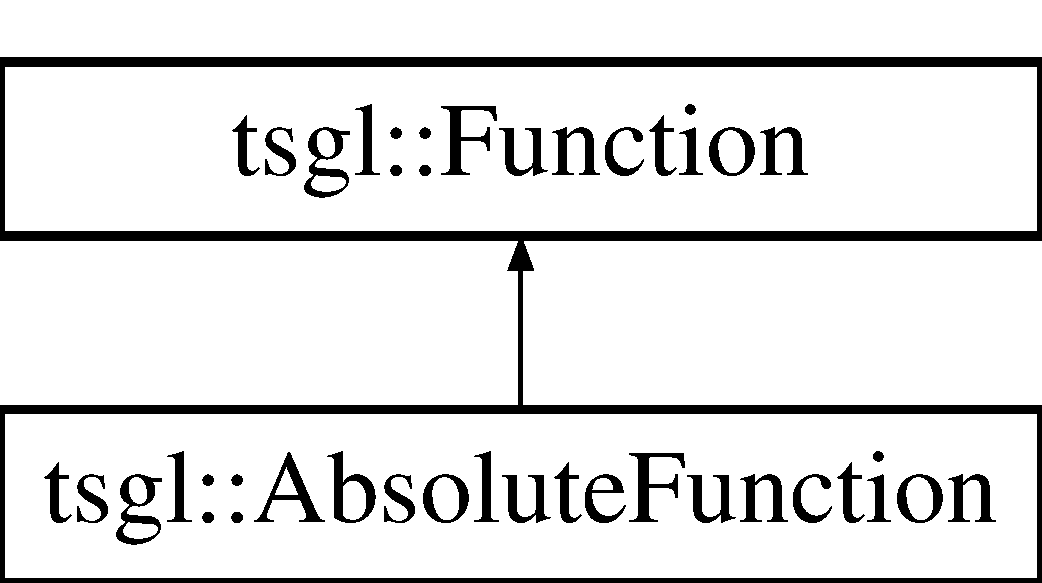
\includegraphics[height=2.000000cm]{classtsgl_1_1_absolute_function}
\end{center}
\end{figure}
\subsection*{\-Public \-Member \-Functions}
\begin{DoxyCompactItemize}
\item 
virtual \-Decimal \hyperlink{classtsgl_1_1_absolute_function_a29b4dd051d17e92b4f2d64b492a6ca19}{value\-At} (\-Decimal x) const 
\begin{DoxyCompactList}\small\item\em \-Method to determine the value of \hyperlink{classtsgl_1_1_absolute_function}{\-Absolute\-Function}. \end{DoxyCompactList}\end{DoxyCompactItemize}


\subsection{\-Detailed \-Description}
\hyperlink{classtsgl_1_1_function}{\-Function} to compute the absolute value of the input. 

\subsection{\-Member \-Function \-Documentation}
\hypertarget{classtsgl_1_1_absolute_function_a29b4dd051d17e92b4f2d64b492a6ca19}{\index{tsgl\-::\-Absolute\-Function@{tsgl\-::\-Absolute\-Function}!value\-At@{value\-At}}
\index{value\-At@{value\-At}!tsgl::AbsoluteFunction@{tsgl\-::\-Absolute\-Function}}
\subsubsection[{value\-At}]{\setlength{\rightskip}{0pt plus 5cm}virtual \-Decimal {\bf tsgl\-::\-Absolute\-Function\-::value\-At} (
\begin{DoxyParamCaption}
\item[{\-Decimal}]{x}
\end{DoxyParamCaption}
) const\hspace{0.3cm}{\ttfamily  \mbox{[}inline, virtual\mbox{]}}}}\label{classtsgl_1_1_absolute_function_a29b4dd051d17e92b4f2d64b492a6ca19}


\-Method to determine the value of \hyperlink{classtsgl_1_1_absolute_function}{\-Absolute\-Function}. 

\begin{DoxyReturn}{\-Returns}
\-The absolute value of $\ast$x$\ast$. 
\end{DoxyReturn}


\-Implements \hyperlink{classtsgl_1_1_function_affb7b3b19a04efefa29a9870d666e912}{tsgl\-::\-Function}.



\-The documentation for this class was generated from the following file\-:\begin{DoxyCompactItemize}
\item 
\-Function.\-h\end{DoxyCompactItemize}

\hypertarget{classtsgl_1_1_array}{\section{tsgl\-:\-:Array$<$ Item $>$ Class Template Reference}
\label{classtsgl_1_1_array}\index{tsgl\-::\-Array$<$ Item $>$@{tsgl\-::\-Array$<$ Item $>$}}
}


Custom internal array used by \hyperlink{classtsgl_1_1_canvas}{Canvas}.  




{\ttfamily \#include $<$Array.\-h$>$}

\subsection*{Public Member Functions}
\begin{DoxyCompactItemize}
\item 
\hyperlink{classtsgl_1_1_array_acc018fe6db37e7eb5df06789de034904}{Array} (unsigned int \hyperlink{classtsgl_1_1_array_a590e6a7c3bbf1470aff97a83f23f83c3}{size})
\begin{DoxyCompactList}\small\item\em \hyperlink{classtsgl_1_1_array}{Array} constructor method. \end{DoxyCompactList}\item 
virtual \hyperlink{classtsgl_1_1_array_aeef4dedf813a5bac862e19c55dee9069}{$\sim$\-Array} ()
\begin{DoxyCompactList}\small\item\em \hyperlink{classtsgl_1_1_array}{Array} destructor method. \end{DoxyCompactList}\item 
\hypertarget{classtsgl_1_1_array_acc5f5148a71c7f606be6cc337116bad6}{void \hyperlink{classtsgl_1_1_array_acc5f5148a71c7f606be6cc337116bad6}{clear} ()}\label{classtsgl_1_1_array_acc5f5148a71c7f606be6cc337116bad6}

\begin{DoxyCompactList}\small\item\em Empties the internal array and resets it, deleting contained objects. \end{DoxyCompactList}\item 
void \hyperlink{classtsgl_1_1_array_afe9d7b1dd294e8c74280b961ac84ac10}{shallow\-Clear} ()
\begin{DoxyCompactList}\small\item\em Empties the internal array but does not delete the objects it contains. \end{DoxyCompactList}\item 
const Item \& \hyperlink{classtsgl_1_1_array_a991ddcad3de14bd96009f4f90b648f6d}{operator\mbox{[}$\,$\mbox{]}} (unsigned int index) const 
\begin{DoxyCompactList}\small\item\em Returns the item at index {\ttfamily index}. \end{DoxyCompactList}\item 
Item \& \hyperlink{classtsgl_1_1_array_ae98fe9dc7998ec3b694150a8f70d8423}{operator\mbox{[}$\,$\mbox{]}} (unsigned int index)
\begin{DoxyCompactList}\small\item\em Returns the item at index {\ttfamily index}. \end{DoxyCompactList}\item 
\hypertarget{classtsgl_1_1_array_a590e6a7c3bbf1470aff97a83f23f83c3}{unsigned int \hyperlink{classtsgl_1_1_array_a590e6a7c3bbf1470aff97a83f23f83c3}{size} () const }\label{classtsgl_1_1_array_a590e6a7c3bbf1470aff97a83f23f83c3}

\begin{DoxyCompactList}\small\item\em Returns the number of items in the internal array. \end{DoxyCompactList}\item 
\hypertarget{classtsgl_1_1_array_a483497b4a309ccbf7e817c7ac1eff95a}{unsigned int \hyperlink{classtsgl_1_1_array_a483497b4a309ccbf7e817c7ac1eff95a}{capacity} () const }\label{classtsgl_1_1_array_a483497b4a309ccbf7e817c7ac1eff95a}

\begin{DoxyCompactList}\small\item\em Returns the maximum amount of items the internal array can store. \end{DoxyCompactList}\item 
\hypertarget{classtsgl_1_1_array_a2676cc880c5638849db5777f33680c9c}{bool \hyperlink{classtsgl_1_1_array_a2676cc880c5638849db5777f33680c9c}{is\-Empty} () const }\label{classtsgl_1_1_array_a2676cc880c5638849db5777f33680c9c}

\begin{DoxyCompactList}\small\item\em Returns true if the internal array contains no items, false otherwise. \end{DoxyCompactList}\item 
Item \hyperlink{classtsgl_1_1_array_aca25dfa4218b2c872d1e1cd2a1a32caa}{push} (Item item)
\begin{DoxyCompactList}\small\item\em Adds the item {\ttfamily item} to the end of the internal array. \end{DoxyCompactList}\end{DoxyCompactItemize}


\subsection{Detailed Description}
\subsubsection*{template$<$typename Item$>$class tsgl\-::\-Array$<$ Item $>$}

Custom internal array used by \hyperlink{classtsgl_1_1_canvas}{Canvas}. 

The \hyperlink{classtsgl_1_1_array}{Array} class manages a custom array for storing shapes to be drawn. It contains utility methods for checking if the internal array is empty, methods for emptying and resetting the internal array, and a subscript operator for accessing individual elements. \begin{DoxyNote}{Note}
The \hyperlink{classtsgl_1_1_array}{Array} has wrap-\/around behavior, behaving similarly to a circular queue. 

If a new shape is pushed into a full \hyperlink{classtsgl_1_1_array}{Array}, the first element is deleted and the pointer to the first element is incremented. 
\end{DoxyNote}


\subsection{Constructor \& Destructor Documentation}
\hypertarget{classtsgl_1_1_array_acc018fe6db37e7eb5df06789de034904}{\index{tsgl\-::\-Array@{tsgl\-::\-Array}!Array@{Array}}
\index{Array@{Array}!tsgl::Array@{tsgl\-::\-Array}}
\subsubsection[{Array}]{\setlength{\rightskip}{0pt plus 5cm}template$<$typename Item$>$ {\bf tsgl\-::\-Array}$<$ Item $>$\-::{\bf Array} (
\begin{DoxyParamCaption}
\item[{unsigned int}]{size}
\end{DoxyParamCaption}
)\hspace{0.3cm}{\ttfamily [inline]}}}\label{classtsgl_1_1_array_acc018fe6db37e7eb5df06789de034904}


\hyperlink{classtsgl_1_1_array}{Array} constructor method. 


\begin{DoxyParams}{Parameters}
{\em size} & The maximum capacity of the \hyperlink{classtsgl_1_1_array}{Array}. \\
\hline
\end{DoxyParams}
\begin{DoxyReturn}{Returns}
An \hyperlink{classtsgl_1_1_array}{Array} with capacity {\ttfamily size}. 
\end{DoxyReturn}
\hypertarget{classtsgl_1_1_array_aeef4dedf813a5bac862e19c55dee9069}{\index{tsgl\-::\-Array@{tsgl\-::\-Array}!$\sim$\-Array@{$\sim$\-Array}}
\index{$\sim$\-Array@{$\sim$\-Array}!tsgl::Array@{tsgl\-::\-Array}}
\subsubsection[{$\sim$\-Array}]{\setlength{\rightskip}{0pt plus 5cm}template$<$typename Item$>$ virtual {\bf tsgl\-::\-Array}$<$ Item $>$\-::$\sim${\bf Array} (
\begin{DoxyParamCaption}
{}
\end{DoxyParamCaption}
)\hspace{0.3cm}{\ttfamily [inline]}, {\ttfamily [virtual]}}}\label{classtsgl_1_1_array_aeef4dedf813a5bac862e19c55dee9069}


\hyperlink{classtsgl_1_1_array}{Array} destructor method. 

Frees up memory allocated to an \hyperlink{classtsgl_1_1_array}{Array} instance. 

\subsection{Member Function Documentation}
\hypertarget{classtsgl_1_1_array_a991ddcad3de14bd96009f4f90b648f6d}{\index{tsgl\-::\-Array@{tsgl\-::\-Array}!operator\mbox{[}$\,$\mbox{]}@{operator[]}}
\index{operator\mbox{[}$\,$\mbox{]}@{operator[]}!tsgl::Array@{tsgl\-::\-Array}}
\subsubsection[{operator[]}]{\setlength{\rightskip}{0pt plus 5cm}template$<$typename Item$>$ const Item\& {\bf tsgl\-::\-Array}$<$ Item $>$\-::operator\mbox{[}$\,$\mbox{]} (
\begin{DoxyParamCaption}
\item[{unsigned int}]{index}
\end{DoxyParamCaption}
) const\hspace{0.3cm}{\ttfamily [inline]}}}\label{classtsgl_1_1_array_a991ddcad3de14bd96009f4f90b648f6d}


Returns the item at index {\ttfamily index}. 


\begin{DoxyParams}{Parameters}
{\em index} & The index of the item in the internal array. \\
\hline
\end{DoxyParams}
\begin{DoxyNote}{Note}
This is the read version of the subscript operator. 
\end{DoxyNote}
\begin{DoxyReturn}{Returns}
The item at index {\ttfamily index}. 
\end{DoxyReturn}
\hypertarget{classtsgl_1_1_array_ae98fe9dc7998ec3b694150a8f70d8423}{\index{tsgl\-::\-Array@{tsgl\-::\-Array}!operator\mbox{[}$\,$\mbox{]}@{operator[]}}
\index{operator\mbox{[}$\,$\mbox{]}@{operator[]}!tsgl::Array@{tsgl\-::\-Array}}
\subsubsection[{operator[]}]{\setlength{\rightskip}{0pt plus 5cm}template$<$typename Item$>$ Item\& {\bf tsgl\-::\-Array}$<$ Item $>$\-::operator\mbox{[}$\,$\mbox{]} (
\begin{DoxyParamCaption}
\item[{unsigned int}]{index}
\end{DoxyParamCaption}
)\hspace{0.3cm}{\ttfamily [inline]}}}\label{classtsgl_1_1_array_ae98fe9dc7998ec3b694150a8f70d8423}


Returns the item at index {\ttfamily index}. 


\begin{DoxyParams}{Parameters}
{\em index} & The index of the item in the internal array. \\
\hline
\end{DoxyParams}
\begin{DoxyNote}{Note}
This is the write version of the subscript operator. 
\end{DoxyNote}
\begin{DoxyReturn}{Returns}
The item at index {\ttfamily index}. 
\end{DoxyReturn}
\hypertarget{classtsgl_1_1_array_aca25dfa4218b2c872d1e1cd2a1a32caa}{\index{tsgl\-::\-Array@{tsgl\-::\-Array}!push@{push}}
\index{push@{push}!tsgl::Array@{tsgl\-::\-Array}}
\subsubsection[{push}]{\setlength{\rightskip}{0pt plus 5cm}template$<$typename Item$>$ Item {\bf tsgl\-::\-Array}$<$ Item $>$\-::push (
\begin{DoxyParamCaption}
\item[{Item}]{item}
\end{DoxyParamCaption}
)\hspace{0.3cm}{\ttfamily [inline]}}}\label{classtsgl_1_1_array_aca25dfa4218b2c872d1e1cd2a1a32caa}


Adds the item {\ttfamily item} to the end of the internal array. 

\begin{DoxyNote}{Note}
If the internal array is full, \hyperlink{classtsgl_1_1_array_aca25dfa4218b2c872d1e1cd2a1a32caa}{push()} will remove the oldest item. 
\end{DoxyNote}

\begin{DoxyParams}{Parameters}
{\em item} & The item to add. \\
\hline
\end{DoxyParams}
\begin{DoxyReturn}{Returns}
The same item. 
\end{DoxyReturn}
\hypertarget{classtsgl_1_1_array_afe9d7b1dd294e8c74280b961ac84ac10}{\index{tsgl\-::\-Array@{tsgl\-::\-Array}!shallow\-Clear@{shallow\-Clear}}
\index{shallow\-Clear@{shallow\-Clear}!tsgl::Array@{tsgl\-::\-Array}}
\subsubsection[{shallow\-Clear}]{\setlength{\rightskip}{0pt plus 5cm}template$<$typename Item$>$ void {\bf tsgl\-::\-Array}$<$ Item $>$\-::shallow\-Clear (
\begin{DoxyParamCaption}
{}
\end{DoxyParamCaption}
)\hspace{0.3cm}{\ttfamily [inline]}}}\label{classtsgl_1_1_array_afe9d7b1dd294e8c74280b961ac84ac10}


Empties the internal array but does not delete the objects it contains. 

\begin{DoxyNote}{Note}
This method doesn't delete the shapes inside of it; it only moves pointers around. 
\end{DoxyNote}
\begin{DoxyWarning}{Warning}
{\bfseries This will result in a memory leak if the objects are not pointed to anywhere else!} 
\end{DoxyWarning}


The documentation for this class was generated from the following file\-:\begin{DoxyCompactItemize}
\item 
Array.\-h\end{DoxyCompactItemize}

\hypertarget{classtsgl_1_1_canvas}{\section{tsgl\-:\-:Canvas Class Reference}
\label{classtsgl_1_1_canvas}\index{tsgl\-::\-Canvas@{tsgl\-::\-Canvas}}
}


A G\-L window with numerous built-\/in, thread-\/safe drawing operations.  




{\ttfamily \#include $<$Canvas.\-h$>$}

Inheritance diagram for tsgl\-:\-:Canvas\-:\begin{figure}[H]
\begin{center}
\leavevmode
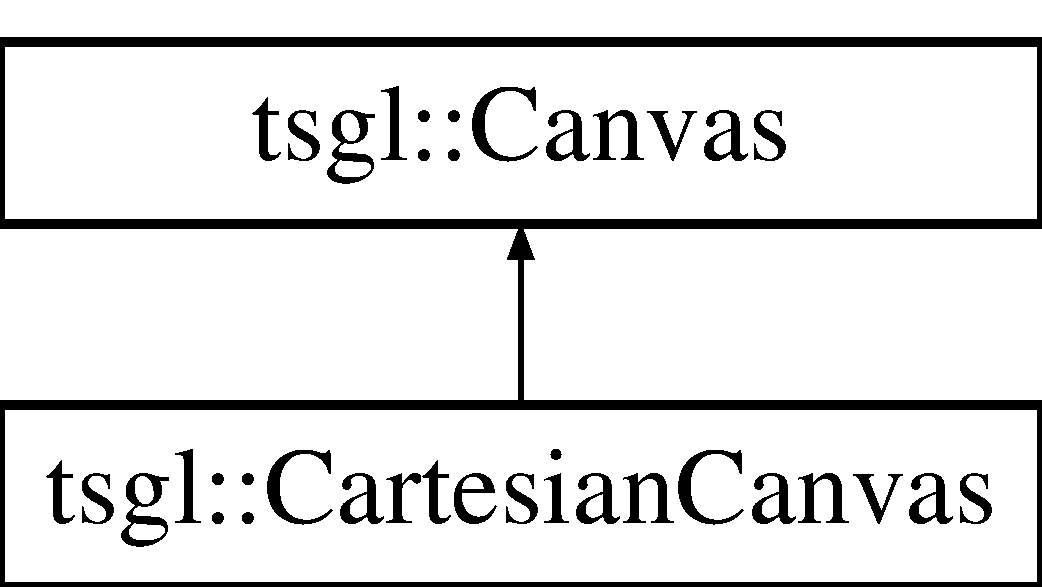
\includegraphics[height=2.000000cm]{classtsgl_1_1_canvas}
\end{center}
\end{figure}
\subsection*{Public Member Functions}
\begin{DoxyCompactItemize}
\item 
\hyperlink{classtsgl_1_1_canvas_ac7e73a23238b067d0b91f73f3af53623}{Canvas} (double timer\-Length=0.\-0f)
\begin{DoxyCompactList}\small\item\em Default \hyperlink{classtsgl_1_1_canvas}{Canvas} constructor method. \end{DoxyCompactList}\item 
\hyperlink{classtsgl_1_1_canvas_a6fac624c804bf5a7169507607d5d876d}{Canvas} (int x, int y, int width, int height, std\-::string title, double timer\-Length=0.\-0f)
\begin{DoxyCompactList}\small\item\em Explicit \hyperlink{classtsgl_1_1_canvas}{Canvas} constructor method. \end{DoxyCompactList}\item 
virtual \hyperlink{classtsgl_1_1_canvas_ab976c3999c68347818d64010b641e14f}{$\sim$\-Canvas} ()
\begin{DoxyCompactList}\small\item\em \hyperlink{classtsgl_1_1_canvas}{Canvas} destructor method. \end{DoxyCompactList}\item 
void \hyperlink{classtsgl_1_1_canvas_a26f2f1acf2b80eee95e42bc13dbc7600}{bind\-To\-Button} (Key button, Action action, void\-Function function)
\begin{DoxyCompactList}\small\item\em Binds a key or button to a function. \end{DoxyCompactList}\item 
void \hyperlink{classtsgl_1_1_canvas_aecd3d94790d2e660db380a5e951ae394}{bind\-To\-Scroll} (std\-::function$<$ void(double, double)$>$ function)
\begin{DoxyCompactList}\small\item\em Binds the mouse wheel to a function. \end{DoxyCompactList}\item 
void \hyperlink{classtsgl_1_1_canvas_abe209d60de2c9b2259ab0588c4e30cef}{clear} ()
\begin{DoxyCompactList}\small\item\em Clears the \hyperlink{classtsgl_1_1_canvas}{Canvas}. \end{DoxyCompactList}\item 
void \hyperlink{classtsgl_1_1_canvas_afaa1250b1da6b48b9c170a0655191938}{close} ()
\begin{DoxyCompactList}\small\item\em Closes the \hyperlink{classtsgl_1_1_canvas}{Canvas} window. \end{DoxyCompactList}\item 
virtual void \hyperlink{classtsgl_1_1_canvas_a2162c16f6aeaee01f8e29696f5818c03}{draw\-Circle} (int x, int y, int radius, int sides, \hyperlink{structtsgl_1_1_color_float}{Color\-Float} color=B\-L\-A\-C\-K, bool filled=true)
\begin{DoxyCompactList}\small\item\em Draws a circle. \end{DoxyCompactList}\item 
virtual void \hyperlink{classtsgl_1_1_canvas_ad98cb8db661ef24279b61c4c11fd29ea}{draw\-Concave\-Polygon} (int size, int xverts\mbox{[}$\,$\mbox{]}, int yverts\mbox{[}$\,$\mbox{]}, \hyperlink{structtsgl_1_1_color_float}{Color\-Float} color\mbox{[}$\,$\mbox{]}, bool filled=true)
\begin{DoxyCompactList}\small\item\em Draws a concave polygon with colored vertices. \end{DoxyCompactList}\item 
virtual void \hyperlink{classtsgl_1_1_canvas_a9cb84248c3559c81e4cb2e0d194b2437}{draw\-Convex\-Polygon} (int size, int xverts\mbox{[}$\,$\mbox{]}, int yverts\mbox{[}$\,$\mbox{]}, \hyperlink{structtsgl_1_1_color_float}{Color\-Float} color\mbox{[}$\,$\mbox{]}, bool filled=true)
\begin{DoxyCompactList}\small\item\em Draws a convex polygon with colored vertices. \end{DoxyCompactList}\item 
virtual void \hyperlink{classtsgl_1_1_canvas_ae94a586629d20b7fabcb402d1c654628}{draw\-Image} (std\-::string filename, int x, int y, int width, int height, float alpha=1.\-0f)
\begin{DoxyCompactList}\small\item\em Draws an image. \end{DoxyCompactList}\item 
virtual void \hyperlink{classtsgl_1_1_canvas_a6e5c605b03a69e615fe4ccee30be1959}{draw\-Line} (int x1, int y1, int x2, int y2, \hyperlink{structtsgl_1_1_color_float}{Color\-Float} color=B\-L\-A\-C\-K)
\begin{DoxyCompactList}\small\item\em Draws a line. \end{DoxyCompactList}\item 
virtual void \hyperlink{classtsgl_1_1_canvas_af17d456eca4ad5a55842f2cf02f48a97}{draw\-Pixel} (int row, int col, \hyperlink{structtsgl_1_1_color_float}{Color\-Float} color=B\-L\-A\-C\-K)
\begin{DoxyCompactList}\small\item\em Draws a single pixel, specified in row,column format. \end{DoxyCompactList}\item 
virtual void \hyperlink{classtsgl_1_1_canvas_a6c17c90cd13f7b0184a25e4acc2b7426}{draw\-Point} (int x, int y, \hyperlink{structtsgl_1_1_color_float}{Color\-Float} color=B\-L\-A\-C\-K)
\begin{DoxyCompactList}\small\item\em Draws a single pixel, specified in x,y format. \end{DoxyCompactList}\item 
virtual void \hyperlink{classtsgl_1_1_canvas_aea792059486ebe6d25d7f81bdadf751d}{draw\-Progress} (\hyperlink{classtsgl_1_1_progress_bar}{Progress\-Bar} $\ast$p)
\begin{DoxyCompactList}\small\item\em Draws a progress bar. \end{DoxyCompactList}\item 
virtual void \hyperlink{classtsgl_1_1_canvas_a752754cd16d14447cb5e5b0438bebf16}{draw\-Rectangle} (int x1, int y1, int x2, int y2, \hyperlink{structtsgl_1_1_color_float}{Color\-Float} color=B\-L\-A\-C\-K, bool filled=true)
\begin{DoxyCompactList}\small\item\em Draws a rectangle. \end{DoxyCompactList}\item 
virtual void \hyperlink{classtsgl_1_1_canvas_a3457e7ebd17fa5003025ff6bcaaeedf6}{draw\-Text} (std\-::string text, int x, int y, unsigned size, \hyperlink{structtsgl_1_1_color_float}{Color\-Float} color=B\-L\-A\-C\-K)
\begin{DoxyCompactList}\small\item\em Draw a string of text. \end{DoxyCompactList}\item 
virtual void \hyperlink{classtsgl_1_1_canvas_a0687604ebe60b37e8685671252172996}{draw\-Text} (std\-::wstring text, int x, int y, unsigned int size, \hyperlink{structtsgl_1_1_color_float}{Color\-Float} color=B\-L\-A\-C\-K)
\begin{DoxyCompactList}\small\item\em Draws a string of text. \end{DoxyCompactList}\item 
virtual void \hyperlink{classtsgl_1_1_canvas_a8abc9ed7d3c55c5d701009040c65000e}{draw\-Triangle} (int x1, int y1, int x2, int y2, int x3, int y3, \hyperlink{structtsgl_1_1_color_float}{Color\-Float} color=B\-L\-A\-C\-K, bool filled=true)
\begin{DoxyCompactList}\small\item\em Draws a triangle. \end{DoxyCompactList}\item 
virtual void \hyperlink{classtsgl_1_1_canvas_a8f570c258a8900178190ec15ac074a57}{draw\-Triangle\-Strip} (int size, int xverts\mbox{[}$\,$\mbox{]}, int yverts\mbox{[}$\,$\mbox{]}, \hyperlink{structtsgl_1_1_color_float}{Color\-Float} color\mbox{[}$\,$\mbox{]}, bool filled=true)
\begin{DoxyCompactList}\small\item\em Draws an arbitrary triangle strip with colored vertices. \end{DoxyCompactList}\item 
\hyperlink{structtsgl_1_1_color_float}{Color\-Float} \hyperlink{classtsgl_1_1_canvas_a2b39e50888d61e88527a66ac0f6ac880}{get\-Background\-Color} ()
\begin{DoxyCompactList}\small\item\em Accessor for the current background color. \end{DoxyCompactList}\item 
int \hyperlink{classtsgl_1_1_canvas_af4f8f2b1abd27316a4a39ae097407d37}{get\-Frame\-Number} ()
\begin{DoxyCompactList}\small\item\em Accessor for the current frame number. \end{DoxyCompactList}\item 
float \hyperlink{classtsgl_1_1_canvas_a1c8ac321138948650a3006f325dfb886}{get\-F\-P\-S} ()
\begin{DoxyCompactList}\small\item\em Accessor for the current F\-P\-S. \end{DoxyCompactList}\item 
bool \hyperlink{classtsgl_1_1_canvas_ada31408e9a96ecb1639f552d8f0de475}{is\-Open} ()
\begin{DoxyCompactList}\small\item\em Accessor for window's closed status. \end{DoxyCompactList}\item 
int \hyperlink{classtsgl_1_1_canvas_a4af9bed83746f998474039185d2a765a}{get\-Mouse\-X} ()
\begin{DoxyCompactList}\small\item\em Accessor for the mouse's x-\/position. \end{DoxyCompactList}\item 
int \hyperlink{classtsgl_1_1_canvas_a7fc8592848aaa14c3ff440d0ed3c9e4f}{get\-Mouse\-Y} ()
\begin{DoxyCompactList}\small\item\em Accessor for the mouse's y-\/position. \end{DoxyCompactList}\item 
\hyperlink{structtsgl_1_1_color_int}{Color\-Int} \hyperlink{classtsgl_1_1_canvas_a1f54dba4b09d248e2611f3409353c2c6}{get\-Pixel} (int row, int col)
\begin{DoxyCompactList}\small\item\em Gets the color of the pixel drawn on the current \hyperlink{classtsgl_1_1_canvas}{Canvas} at the given screen coordinates, specified in row,column format. \end{DoxyCompactList}\item 
\hyperlink{structtsgl_1_1_color_int}{Color\-Int} \hyperlink{classtsgl_1_1_canvas_aa31883b3c9b09006cf82b270ad7a0a9f}{get\-Point} (int x, int y)
\begin{DoxyCompactList}\small\item\em Gets the color of the pixel drawn on the current \hyperlink{classtsgl_1_1_canvas}{Canvas} at the given screen coordinates, specified in x,y format. \end{DoxyCompactList}\item 
unsigned int \hyperlink{classtsgl_1_1_canvas_a8f0819f368b41b147f1a7f560a7af6a4}{get\-Reps} () const 
\begin{DoxyCompactList}\small\item\em Accessor for the number of theoretical draw cycles that have elapsed. \end{DoxyCompactList}\item 
uint8\-\_\-t $\ast$ \hyperlink{classtsgl_1_1_canvas_a71f072dd82ca3b5cecfd65cde6d8a226}{get\-Screen\-Buffer} ()
\begin{DoxyCompactList}\small\item\em Accessor for the \hyperlink{classtsgl_1_1_canvas}{Canvas}'s currently drawn image. \end{DoxyCompactList}\item 
double \hyperlink{classtsgl_1_1_canvas_aef462ab48e59571b9c88076bbdc8f0b3}{get\-Time} ()
\begin{DoxyCompactList}\small\item\em Accessor for the time since the \hyperlink{classtsgl_1_1_canvas}{Canvas} was initialized. \end{DoxyCompactList}\item 
double \hyperlink{classtsgl_1_1_canvas_a8786d28042b767f5c075361100227af4}{get\-Time\-Between\-Sleeps} () const 
\begin{DoxyCompactList}\small\item\em Accessor that gets the time between two sleep times of the internal drawing timer of a \hyperlink{classtsgl_1_1_canvas}{Canvas} object. \end{DoxyCompactList}\item 
int \hyperlink{classtsgl_1_1_canvas_ad740ebe5d6bd69ab79cde3e84f369f35}{get\-Window\-Height} ()
\begin{DoxyCompactList}\small\item\em Accessor for the \hyperlink{classtsgl_1_1_canvas}{Canvas}'s window height. \end{DoxyCompactList}\item 
int \hyperlink{classtsgl_1_1_canvas_a086a0322f4a6ab27da6929b1aa0593af}{get\-Window\-Width} ()
\begin{DoxyCompactList}\small\item\em Accessor for the \hyperlink{classtsgl_1_1_canvas}{Canvas}'s window width. \end{DoxyCompactList}\item 
int \hyperlink{classtsgl_1_1_canvas_a011ce2354d4565f9d2a323411a47d52d}{get\-Window\-X} ()
\begin{DoxyCompactList}\small\item\em Accessor for the \hyperlink{classtsgl_1_1_canvas}{Canvas}'s x-\/position. \end{DoxyCompactList}\item 
int \hyperlink{classtsgl_1_1_canvas_ad6e98d17d3e43d79628a3bd05221ee8b}{get\-Window\-Y} ()
\begin{DoxyCompactList}\small\item\em Accessor for the \hyperlink{classtsgl_1_1_canvas}{Canvas}'s y-\/position. \end{DoxyCompactList}\item 
void \hyperlink{classtsgl_1_1_canvas_aa499851e5e4b97bb99ca4fb3d633c17e}{handle\-I\-O} ()
\begin{DoxyCompactList}\small\item\em Manually handles keyboard/mouse I/\-O. \end{DoxyCompactList}\item 
void \hyperlink{classtsgl_1_1_canvas_abe021ab5148cc1327523689bced0f35a}{pause\-Drawing} ()
\begin{DoxyCompactList}\small\item\em Pauses the rendering thread of the \hyperlink{classtsgl_1_1_canvas}{Canvas}. \end{DoxyCompactList}\item 
void \hyperlink{classtsgl_1_1_canvas_a47436daa39473ddb4044bac7b3b27151}{record\-For\-Num\-Frames} (unsigned int num\-\_\-frames)
\begin{DoxyCompactList}\small\item\em Records the \hyperlink{classtsgl_1_1_canvas}{Canvas} for a specified number of frames. \end{DoxyCompactList}\item 
void \hyperlink{classtsgl_1_1_canvas_ada6403439b583910d27e497148da5f2e}{reset} ()
\begin{DoxyCompactList}\small\item\em Resets the internal drawing timer of a \hyperlink{classtsgl_1_1_canvas}{Canvas} instance. \end{DoxyCompactList}\item 
void \hyperlink{classtsgl_1_1_canvas_a56bf3c6e4eb7b06015d1c115aaa143f8}{resume\-Drawing} ()
\begin{DoxyCompactList}\small\item\em Resumes the rendering thread of the \hyperlink{classtsgl_1_1_canvas}{Canvas}. \end{DoxyCompactList}\item 
virtual void \hyperlink{classtsgl_1_1_canvas_a5f3f00d6c380a662a239077456045502}{run} (void($\ast$my\-Function)(\hyperlink{classtsgl_1_1_canvas}{Canvas} \&))
\begin{DoxyCompactList}\small\item\em Start the \hyperlink{classtsgl_1_1_canvas}{Canvas}, run a function on it, and wait for the user to close it. \end{DoxyCompactList}\item 
virtual void \hyperlink{classtsgl_1_1_canvas_a62ec8be88bea1905cdb6855138ef3cb1}{run} (void($\ast$my\-Function)(\hyperlink{classtsgl_1_1_canvas}{Canvas} \&, int), int i)
\begin{DoxyCompactList}\small\item\em Overload for \hyperlink{classtsgl_1_1_canvas_a5f3f00d6c380a662a239077456045502}{run()} \end{DoxyCompactList}\item 
virtual void \hyperlink{classtsgl_1_1_canvas_a67b341ead1fde0a692281d2b1f67be1e}{run} (void($\ast$my\-Function)(\hyperlink{classtsgl_1_1_canvas}{Canvas} \&, unsigned), unsigned u)
\begin{DoxyCompactList}\small\item\em Overload for \hyperlink{classtsgl_1_1_canvas_a5f3f00d6c380a662a239077456045502}{run()} \end{DoxyCompactList}\item 
virtual void \hyperlink{classtsgl_1_1_canvas_a768c10737f9590a25d8e66dcc7137d9b}{run} (void($\ast$my\-Function)(\hyperlink{classtsgl_1_1_canvas}{Canvas} \&, int, int), int i1, int i2)
\begin{DoxyCompactList}\small\item\em Overload for \hyperlink{classtsgl_1_1_canvas_a5f3f00d6c380a662a239077456045502}{run()} \end{DoxyCompactList}\item 
virtual void \hyperlink{classtsgl_1_1_canvas_ab146e6cf9f7f19a047c20c02a0eb30f9}{run} (void($\ast$my\-Function)(\hyperlink{classtsgl_1_1_canvas}{Canvas} \&, unsigned, unsigned), unsigned u1, unsigned u2)
\begin{DoxyCompactList}\small\item\em Overload for \hyperlink{classtsgl_1_1_canvas_a5f3f00d6c380a662a239077456045502}{run()} \end{DoxyCompactList}\item 
virtual void \hyperlink{classtsgl_1_1_canvas_a2eeece8d4c4453ec7b4b53e209004559}{run} (void($\ast$my\-Function)(\hyperlink{classtsgl_1_1_canvas}{Canvas} \&, std\-::string), std\-::string s)
\begin{DoxyCompactList}\small\item\em Overload for \hyperlink{classtsgl_1_1_canvas_a5f3f00d6c380a662a239077456045502}{run()} \end{DoxyCompactList}\item 
virtual void \hyperlink{classtsgl_1_1_canvas_ac507bbbf60328de2fc99f93cd37d04ec}{run} (void($\ast$my\-Function)(\hyperlink{classtsgl_1_1_canvas}{Canvas} \&, int, std\-::string), int i, std\-::string s)
\begin{DoxyCompactList}\small\item\em Overload for \hyperlink{classtsgl_1_1_canvas_a5f3f00d6c380a662a239077456045502}{run()} \end{DoxyCompactList}\item 
virtual void \hyperlink{classtsgl_1_1_canvas_aafed71cba89b059629647e77ba23ff2b}{run} (void($\ast$my\-Function)(\hyperlink{classtsgl_1_1_canvas}{Canvas} \&, std\-::string, int), std\-::string s, int i)
\begin{DoxyCompactList}\small\item\em Overload for \hyperlink{classtsgl_1_1_canvas_a5f3f00d6c380a662a239077456045502}{run()} \end{DoxyCompactList}\item 
void \hyperlink{classtsgl_1_1_canvas_abb668fe42e2fe7f269b255152df959d8}{set\-Background\-Color} (\hyperlink{structtsgl_1_1_color_float}{Color\-Float} color)
\begin{DoxyCompactList}\small\item\em Mutator for the background color. \end{DoxyCompactList}\item 
void \hyperlink{classtsgl_1_1_canvas_a692edf8e37c7714cdf2a58ea530c63e9}{set\-Font} (std\-::string filename)
\begin{DoxyCompactList}\small\item\em Mutator for the currently loaded font. \end{DoxyCompactList}\item 
void \hyperlink{classtsgl_1_1_canvas_a8722c579dfa55a45e139bfeb269d73ff}{set\-Show\-F\-P\-S} (bool b)
\begin{DoxyCompactList}\small\item\em Mutator for showing the F\-P\-S. \end{DoxyCompactList}\item 
void \hyperlink{classtsgl_1_1_canvas_a2604fa056d4541f918ccf447eda1f3cf}{sleep} ()
\begin{DoxyCompactList}\small\item\em Sleeps the calling thread to sync with the \hyperlink{classtsgl_1_1_canvas}{Canvas}. \end{DoxyCompactList}\item 
void \hyperlink{classtsgl_1_1_canvas_a6674cc86b9a54b6a564021fddce47e36}{sleep\-For} (float seconds)
\begin{DoxyCompactList}\small\item\em Sleeps the calling thread for a set amount of time. \end{DoxyCompactList}\item 
int \hyperlink{classtsgl_1_1_canvas_a654315f9b08a9b3b072eebf4b4d8ae89}{start} ()
\begin{DoxyCompactList}\small\item\em Opens the \hyperlink{classtsgl_1_1_canvas}{Canvas}. \end{DoxyCompactList}\item 
void \hyperlink{classtsgl_1_1_canvas_a46cd37a9f2a146e57b4e0273faf6485c}{stop} ()
\begin{DoxyCompactList}\small\item\em Begins the process of closing the \hyperlink{classtsgl_1_1_canvas}{Canvas}. \end{DoxyCompactList}\item 
void \hyperlink{classtsgl_1_1_canvas_ac6035d87aa3bf077031bc0bb6f419b17}{stop\-Recording} ()
\begin{DoxyCompactList}\small\item\em Stops recording the \hyperlink{classtsgl_1_1_canvas}{Canvas}. \end{DoxyCompactList}\item 
void \hyperlink{classtsgl_1_1_canvas_ac035f43763b198f6915a0772973a5ea9}{take\-Screen\-Shot} ()
\begin{DoxyCompactList}\small\item\em Takes a screenshot. \end{DoxyCompactList}\item 
int \hyperlink{classtsgl_1_1_canvas_a39e69fd4d1ad8cf0e22ecea12f1ddf08}{wait} ()
\begin{DoxyCompactList}\small\item\em Waits for the user to close the \hyperlink{classtsgl_1_1_canvas}{Canvas}. \end{DoxyCompactList}\end{DoxyCompactItemize}
\subsection*{Static Public Member Functions}
\begin{DoxyCompactItemize}
\item 
static int \hyperlink{classtsgl_1_1_canvas_a664b101f972845eaf5fdc4d9e664e623}{get\-Display\-Height} ()
\begin{DoxyCompactList}\small\item\em Accessor for the height of the user's primary monitor. \end{DoxyCompactList}\item 
static int \hyperlink{classtsgl_1_1_canvas_abbe5c392cac2320fecf1f2751afb207c}{get\-Display\-Width} ()
\begin{DoxyCompactList}\small\item\em Accessor for the width of the user's primary monitor. \end{DoxyCompactList}\item 
\hypertarget{classtsgl_1_1_canvas_a3365d92635f650cca2eda69812bef60b}{static void \hyperlink{classtsgl_1_1_canvas_a3365d92635f650cca2eda69812bef60b}{run\-Tests} ()}\label{classtsgl_1_1_canvas_a3365d92635f650cca2eda69812bef60b}

\begin{DoxyCompactList}\small\item\em Runs unit tests for the \hyperlink{classtsgl_1_1_canvas}{Canvas}. \end{DoxyCompactList}\end{DoxyCompactItemize}
\subsection*{Protected Member Functions}
\begin{DoxyCompactItemize}
\item 
\hypertarget{classtsgl_1_1_canvas_a560e3f64f3b2e5a7af8a8d7b92d8e660}{void {\bfseries draw\-Shape} (\hyperlink{classtsgl_1_1_shape}{Shape} $\ast$s)}\label{classtsgl_1_1_canvas_a560e3f64f3b2e5a7af8a8d7b92d8e660}

\end{DoxyCompactItemize}
\subsection*{Protected Attributes}
\begin{DoxyCompactItemize}
\item 
\hypertarget{classtsgl_1_1_canvas_a1558f2f09228ccaf0d46cec233a2dac7}{bool {\bfseries ati\-Card}}\label{classtsgl_1_1_canvas_a1558f2f09228ccaf0d46cec233a2dac7}

\end{DoxyCompactItemize}


\subsection{Detailed Description}
A G\-L window with numerous built-\/in, thread-\/safe drawing operations. 

\hyperlink{classtsgl_1_1_canvas}{Canvas} provides an easy-\/to-\/set-\/up, easy-\/to-\/use class for drawing various shapes.

Using S\-T\-B, \hyperlink{classtsgl_1_1_canvas}{Canvas} also supports the drawing of images.

On top of being easy to use, \hyperlink{classtsgl_1_1_canvas}{Canvas} is also thread-\/safe, so any number of images may be drawn at once. \begin{DoxyNote}{Note}
{\bfseries O\-S X\-:} Due to the way O\-S X handles I/\-O, either \hyperlink{classtsgl_1_1_canvas_a2604fa056d4541f918ccf447eda1f3cf}{sleep()} or \hyperlink{classtsgl_1_1_canvas_aa499851e5e4b97bb99ca4fb3d633c17e}{handle\-I\-O()} must be manually called whenever the user wants to handle any input/output events (keyboard/mouse presses). Whenever a window is created using Open\-G\-L, O\-S X requires the main thread to handle I/\-O calls. 

{\bfseries O\-S X\-:} O\-S X also uses p\-\_\-thread instead of std\-::thread for threading. 
\end{DoxyNote}
\begin{DoxyRefDesc}{Bug}
\item[\hyperlink{bug__bug000001}{Bug}]{\bfseries Linux\-:} X forwarding does not work properly with T\-S\-G\-L. \end{DoxyRefDesc}


\subsection{Constructor \& Destructor Documentation}
\hypertarget{classtsgl_1_1_canvas_ac7e73a23238b067d0b91f73f3af53623}{\index{tsgl\-::\-Canvas@{tsgl\-::\-Canvas}!Canvas@{Canvas}}
\index{Canvas@{Canvas}!tsgl::Canvas@{tsgl\-::\-Canvas}}
\subsubsection[{Canvas}]{\setlength{\rightskip}{0pt plus 5cm}tsgl\-::\-Canvas\-::\-Canvas (
\begin{DoxyParamCaption}
\item[{double}]{timer\-Length = {\ttfamily 0.0f}}
\end{DoxyParamCaption}
)}}\label{classtsgl_1_1_canvas_ac7e73a23238b067d0b91f73f3af53623}


Default \hyperlink{classtsgl_1_1_canvas}{Canvas} constructor method. 

This is the default constructor for the \hyperlink{classtsgl_1_1_canvas}{Canvas} class. 
\begin{DoxyParams}{Parameters}
{\em timer\-Length} & The minimum number of seconds between draw cycles for the \hyperlink{classtsgl_1_1_canvas}{Canvas}. A value less than or equal to 0 sets it to automatic. \\
\hline
\end{DoxyParams}
\begin{DoxyReturn}{Returns}
A new \hyperlink{classtsgl_1_1_canvas}{Canvas} in the middle of the screen with no title. The created \hyperlink{classtsgl_1_1_canvas}{Canvas} will take up approximately 90\% of the monitor's height, and will have a 4\-:3 aspect ratio. 
\end{DoxyReturn}
\hypertarget{classtsgl_1_1_canvas_a6fac624c804bf5a7169507607d5d876d}{\index{tsgl\-::\-Canvas@{tsgl\-::\-Canvas}!Canvas@{Canvas}}
\index{Canvas@{Canvas}!tsgl::Canvas@{tsgl\-::\-Canvas}}
\subsubsection[{Canvas}]{\setlength{\rightskip}{0pt plus 5cm}tsgl\-::\-Canvas\-::\-Canvas (
\begin{DoxyParamCaption}
\item[{int}]{x, }
\item[{int}]{y, }
\item[{int}]{width, }
\item[{int}]{height, }
\item[{std\-::string}]{title, }
\item[{double}]{timer\-Length = {\ttfamily 0.0f}}
\end{DoxyParamCaption}
)}}\label{classtsgl_1_1_canvas_a6fac624c804bf5a7169507607d5d876d}


Explicit \hyperlink{classtsgl_1_1_canvas}{Canvas} constructor method. 

This is the explicit constructor for the \hyperlink{classtsgl_1_1_canvas}{Canvas} class. 
\begin{DoxyParams}{Parameters}
{\em x} & The x position of the \hyperlink{classtsgl_1_1_canvas}{Canvas} window. \\
\hline
{\em y} & The y position of the \hyperlink{classtsgl_1_1_canvas}{Canvas} window. \\
\hline
{\em width} & The x dimension of the \hyperlink{classtsgl_1_1_canvas}{Canvas} window. \\
\hline
{\em height} & The y dimension of the \hyperlink{classtsgl_1_1_canvas}{Canvas} window. \\
\hline
{\em title} & The title of the window. \\
\hline
{\em timer\-Length} & The minimum number of seconds between draw cycles for the \hyperlink{classtsgl_1_1_canvas}{Canvas}. A value less than or equal to 0 sets it to automatic. \\
\hline
\end{DoxyParams}
\begin{DoxyReturn}{Returns}
A new \hyperlink{classtsgl_1_1_canvas}{Canvas} with the specified position, dimensions, title, and draw cycle length. 
\end{DoxyReturn}
\hypertarget{classtsgl_1_1_canvas_ab976c3999c68347818d64010b641e14f}{\index{tsgl\-::\-Canvas@{tsgl\-::\-Canvas}!$\sim$\-Canvas@{$\sim$\-Canvas}}
\index{$\sim$\-Canvas@{$\sim$\-Canvas}!tsgl::Canvas@{tsgl\-::\-Canvas}}
\subsubsection[{$\sim$\-Canvas}]{\setlength{\rightskip}{0pt plus 5cm}tsgl\-::\-Canvas\-::$\sim$\-Canvas (
\begin{DoxyParamCaption}
{}
\end{DoxyParamCaption}
)\hspace{0.3cm}{\ttfamily [virtual]}}}\label{classtsgl_1_1_canvas_ab976c3999c68347818d64010b641e14f}


\hyperlink{classtsgl_1_1_canvas}{Canvas} destructor method. 

This is the destructor for the \hyperlink{classtsgl_1_1_canvas}{Canvas} class.

Frees up memory that was allocated to a \hyperlink{classtsgl_1_1_canvas}{Canvas} instance. 

\subsection{Member Function Documentation}
\hypertarget{classtsgl_1_1_canvas_a26f2f1acf2b80eee95e42bc13dbc7600}{\index{tsgl\-::\-Canvas@{tsgl\-::\-Canvas}!bind\-To\-Button@{bind\-To\-Button}}
\index{bind\-To\-Button@{bind\-To\-Button}!tsgl::Canvas@{tsgl\-::\-Canvas}}
\subsubsection[{bind\-To\-Button}]{\setlength{\rightskip}{0pt plus 5cm}void tsgl\-::\-Canvas\-::bind\-To\-Button (
\begin{DoxyParamCaption}
\item[{Key}]{button, }
\item[{Action}]{action, }
\item[{void\-Function}]{function}
\end{DoxyParamCaption}
)}}\label{classtsgl_1_1_canvas_a26f2f1acf2b80eee95e42bc13dbc7600}


Binds a key or button to a function. 

This function binds a key or mouse button to a function pointer.

Upon pressing or releasing the given key, \hyperlink{classtsgl_1_1_canvas}{Canvas} will call the specified function. 
\begin{DoxyParams}{Parameters}
{\em button} & The key or button to bind, as specified in \hyperlink{_keynums_8h_source}{Keynums.\-h}. \\
\hline
{\em action} & The action to look out for (T\-S\-G\-L\-\_\-\-P\-R\-E\-S\-S or T\-S\-G\-L\-\_\-\-R\-E\-L\-E\-A\-S\-E). \\
\hline
{\em function} & The function to call upon action {\ttfamily a} on button. \\
\hline
\end{DoxyParams}
\begin{DoxyWarning}{Warning}
{\bfseries T\-S\-G\-L\-\_\-\-K\-E\-Y\-\_\-\-E\-S\-C\-A\-P\-E is automatically bound to closing the window. Overriding T\-S\-G\-L\-\_\-\-K\-E\-Y\-\_\-\-E\-S\-C\-A\-P\-E will likely make you unable to close the window through the escape key.} 
\end{DoxyWarning}
\hypertarget{classtsgl_1_1_canvas_aecd3d94790d2e660db380a5e951ae394}{\index{tsgl\-::\-Canvas@{tsgl\-::\-Canvas}!bind\-To\-Scroll@{bind\-To\-Scroll}}
\index{bind\-To\-Scroll@{bind\-To\-Scroll}!tsgl::Canvas@{tsgl\-::\-Canvas}}
\subsubsection[{bind\-To\-Scroll}]{\setlength{\rightskip}{0pt plus 5cm}void tsgl\-::\-Canvas\-::bind\-To\-Scroll (
\begin{DoxyParamCaption}
\item[{std\-::function$<$ void(double, double)$>$}]{function}
\end{DoxyParamCaption}
)}}\label{classtsgl_1_1_canvas_aecd3d94790d2e660db380a5e951ae394}


Binds the mouse wheel to a function. 

This function binds the mouse wheel to a function pointer.

Upon scrolling, \hyperlink{classtsgl_1_1_canvas}{Canvas} will call the specified function. 
\begin{DoxyParams}{Parameters}
{\em function} & A function taking x and y parameters to be called when the mouse is scrolled. \\
\hline
\end{DoxyParams}
\hypertarget{classtsgl_1_1_canvas_abe209d60de2c9b2259ab0588c4e30cef}{\index{tsgl\-::\-Canvas@{tsgl\-::\-Canvas}!clear@{clear}}
\index{clear@{clear}!tsgl::Canvas@{tsgl\-::\-Canvas}}
\subsubsection[{clear}]{\setlength{\rightskip}{0pt plus 5cm}void tsgl\-::\-Canvas\-::clear (
\begin{DoxyParamCaption}
{}
\end{DoxyParamCaption}
)}}\label{classtsgl_1_1_canvas_abe209d60de2c9b2259ab0588c4e30cef}


Clears the \hyperlink{classtsgl_1_1_canvas}{Canvas}. 

This function clears the screen to the color specified in \hyperlink{classtsgl_1_1_canvas_abb668fe42e2fe7f269b255152df959d8}{set\-Background\-Color()}. 

Referenced by tsgl\-::\-Spectrogram\-::draw().

\hypertarget{classtsgl_1_1_canvas_afaa1250b1da6b48b9c170a0655191938}{\index{tsgl\-::\-Canvas@{tsgl\-::\-Canvas}!close@{close}}
\index{close@{close}!tsgl::Canvas@{tsgl\-::\-Canvas}}
\subsubsection[{close}]{\setlength{\rightskip}{0pt plus 5cm}void tsgl\-::\-Canvas\-::close (
\begin{DoxyParamCaption}
{}
\end{DoxyParamCaption}
)}}\label{classtsgl_1_1_canvas_afaa1250b1da6b48b9c170a0655191938}


Closes the \hyperlink{classtsgl_1_1_canvas}{Canvas} window. 

This function tells the \hyperlink{classtsgl_1_1_canvas}{Canvas} to stop rendering and to close its rendering window.

Any threads that have called \hyperlink{classtsgl_1_1_canvas_a39e69fd4d1ad8cf0e22ecea12f1ddf08}{wait()} will continue. \begin{DoxySeeAlso}{See Also}
\hyperlink{classtsgl_1_1_canvas_a654315f9b08a9b3b072eebf4b4d8ae89}{start()}, \hyperlink{classtsgl_1_1_canvas_a46cd37a9f2a146e57b4e0273faf6485c}{stop()}, \hyperlink{classtsgl_1_1_canvas_a39e69fd4d1ad8cf0e22ecea12f1ddf08}{wait()} 
\end{DoxySeeAlso}


Referenced by tsgl\-::\-Visual\-Task\-Queue\-::close(), and stop().

\hypertarget{classtsgl_1_1_canvas_a2162c16f6aeaee01f8e29696f5818c03}{\index{tsgl\-::\-Canvas@{tsgl\-::\-Canvas}!draw\-Circle@{draw\-Circle}}
\index{draw\-Circle@{draw\-Circle}!tsgl::Canvas@{tsgl\-::\-Canvas}}
\subsubsection[{draw\-Circle}]{\setlength{\rightskip}{0pt plus 5cm}void tsgl\-::\-Canvas\-::draw\-Circle (
\begin{DoxyParamCaption}
\item[{int}]{x, }
\item[{int}]{y, }
\item[{int}]{radius, }
\item[{int}]{sides, }
\item[{{\bf Color\-Float}}]{color = {\ttfamily BLACK}, }
\item[{bool}]{filled = {\ttfamily true}}
\end{DoxyParamCaption}
)\hspace{0.3cm}{\ttfamily [virtual]}}}\label{classtsgl_1_1_canvas_a2162c16f6aeaee01f8e29696f5818c03}


Draws a circle. 

This function draws a circle with the given center, radius, resolution (number of sides), color, and fill status. 
\begin{DoxyParams}{Parameters}
{\em x} & The x coordinate of the circle's center. \\
\hline
{\em y} & The y coordinate of the circle's center. \\
\hline
{\em radius} & The radius of the circle in pixels. \\
\hline
{\em sides} & The number of sides to use in the circle. \\
\hline
{\em color} & The color of the circle (set to B\-L\-A\-C\-K by default). \\
\hline
{\em filled} & Whether the circle should be filled (set to true by default). \\
\hline
\end{DoxyParams}


Referenced by tsgl\-::\-Cartesian\-Canvas\-::draw\-Circle().

\hypertarget{classtsgl_1_1_canvas_ad98cb8db661ef24279b61c4c11fd29ea}{\index{tsgl\-::\-Canvas@{tsgl\-::\-Canvas}!draw\-Concave\-Polygon@{draw\-Concave\-Polygon}}
\index{draw\-Concave\-Polygon@{draw\-Concave\-Polygon}!tsgl::Canvas@{tsgl\-::\-Canvas}}
\subsubsection[{draw\-Concave\-Polygon}]{\setlength{\rightskip}{0pt plus 5cm}void tsgl\-::\-Canvas\-::draw\-Concave\-Polygon (
\begin{DoxyParamCaption}
\item[{int}]{size, }
\item[{int}]{xverts\mbox{[}$\,$\mbox{]}, }
\item[{int}]{yverts\mbox{[}$\,$\mbox{]}, }
\item[{{\bf Color\-Float}}]{color\mbox{[}$\,$\mbox{]}, }
\item[{bool}]{filled = {\ttfamily true}}
\end{DoxyParamCaption}
)\hspace{0.3cm}{\ttfamily [virtual]}}}\label{classtsgl_1_1_canvas_ad98cb8db661ef24279b61c4c11fd29ea}


Draws a concave polygon with colored vertices. 

This function draws a \hyperlink{classtsgl_1_1_concave_polygon}{Concave\-Polygon} with the given vertex data, specified as the outer perimeter of the polygon. 
\begin{DoxyParams}{Parameters}
{\em size} & The number of vertices in the polygon. \\
\hline
{\em xverts} & An array of x positions of said vertices. \\
\hline
{\em yverts} & An array of y positions of said vertices. \\
\hline
{\em color} & An array of colors for the said vertices. \\
\hline
{\em filled} & Whether the Concave polygon should be filled in or not (set to true by default). \\
\hline
\end{DoxyParams}
\begin{DoxyWarning}{Warning}
{\bfseries This function is significantly slower than \hyperlink{classtsgl_1_1_canvas_a9cb84248c3559c81e4cb2e0d194b2437}{draw\-Convex\-Polygon()}. It is not recommended that you draw convex polygons with this function. }
\end{DoxyWarning}
\begin{DoxySeeAlso}{See Also}
{\bfseries  \hyperlink{classtsgl_1_1_canvas_a9cb84248c3559c81e4cb2e0d194b2437}{draw\-Convex\-Polygon()}. }
\end{DoxySeeAlso}


Referenced by tsgl\-::\-Cartesian\-Canvas\-::draw\-Concave\-Polygon().

\hypertarget{classtsgl_1_1_canvas_a9cb84248c3559c81e4cb2e0d194b2437}{\index{tsgl\-::\-Canvas@{tsgl\-::\-Canvas}!draw\-Convex\-Polygon@{draw\-Convex\-Polygon}}
\index{draw\-Convex\-Polygon@{draw\-Convex\-Polygon}!tsgl::Canvas@{tsgl\-::\-Canvas}}
\subsubsection[{draw\-Convex\-Polygon}]{\setlength{\rightskip}{0pt plus 5cm}void tsgl\-::\-Canvas\-::draw\-Convex\-Polygon (
\begin{DoxyParamCaption}
\item[{int}]{size, }
\item[{int}]{xverts\mbox{[}$\,$\mbox{]}, }
\item[{int}]{yverts\mbox{[}$\,$\mbox{]}, }
\item[{{\bf Color\-Float}}]{color\mbox{[}$\,$\mbox{]}, }
\item[{bool}]{filled = {\ttfamily true}}
\end{DoxyParamCaption}
)\hspace{0.3cm}{\ttfamily [virtual]}}}\label{classtsgl_1_1_canvas_a9cb84248c3559c81e4cb2e0d194b2437}


Draws a convex polygon with colored vertices. 

This function draws a \hyperlink{classtsgl_1_1_convex_polygon}{Convex\-Polygon} with the given vertex data, specified as the outer perimeter of the polygon. 
\begin{DoxyParams}{Parameters}
{\em size} & The number of vertices in the polygon. \\
\hline
{\em xverts} & An array of the x positions of said vertices. \\
\hline
{\em yverts} & An array of the y positions of said vertices. \\
\hline
{\em color} & An array of colors for the said vertices. \\
\hline
{\em filled} & Whether the \hyperlink{classtsgl_1_1_convex_polygon}{Convex\-Polygon} should be filled in or not (set to true by default). \\
\hline
\end{DoxyParams}
\begin{DoxyNote}{Note}
The difference between a convex polygon and a concave polygon is that a convex polygon has all interior angles less than 180 degrees ( see \href{http://www.mathopenref.com/polygonconvex.html}{\tt http\-://www.\-mathopenref.\-com/polygonconvex.\-html} ). 
\end{DoxyNote}


Referenced by tsgl\-::\-Spectrogram\-::draw(), and tsgl\-::\-Cartesian\-Canvas\-::draw\-Convex\-Polygon().

\hypertarget{classtsgl_1_1_canvas_ae94a586629d20b7fabcb402d1c654628}{\index{tsgl\-::\-Canvas@{tsgl\-::\-Canvas}!draw\-Image@{draw\-Image}}
\index{draw\-Image@{draw\-Image}!tsgl::Canvas@{tsgl\-::\-Canvas}}
\subsubsection[{draw\-Image}]{\setlength{\rightskip}{0pt plus 5cm}void tsgl\-::\-Canvas\-::draw\-Image (
\begin{DoxyParamCaption}
\item[{std\-::string}]{filename, }
\item[{int}]{x, }
\item[{int}]{y, }
\item[{int}]{width, }
\item[{int}]{height, }
\item[{float}]{alpha = {\ttfamily 1.0f}}
\end{DoxyParamCaption}
)\hspace{0.3cm}{\ttfamily [virtual]}}}\label{classtsgl_1_1_canvas_ae94a586629d20b7fabcb402d1c654628}


Draws an image. 

This function draws an \hyperlink{classtsgl_1_1_image}{Image} with the given coordinates and dimensions. 
\begin{DoxyParams}{Parameters}
{\em filename} & The name of the file to load the image from. \\
\hline
{\em x} & The x coordinate of the \hyperlink{classtsgl_1_1_image}{Image}'s left edge. \\
\hline
{\em y} & The y coordinate of the \hyperlink{classtsgl_1_1_image}{Image}'s top edge. \\
\hline
{\em width} & The width of the \hyperlink{classtsgl_1_1_image}{Image}. \\
\hline
{\em height} & The height of the \hyperlink{classtsgl_1_1_image}{Image}. \\
\hline
{\em alpha} & The alpha with which to draw the \hyperlink{classtsgl_1_1_image}{Image} \\
\hline
\end{DoxyParams}


Referenced by tsgl\-::\-Cartesian\-Canvas\-::draw\-Image().

\hypertarget{classtsgl_1_1_canvas_a6e5c605b03a69e615fe4ccee30be1959}{\index{tsgl\-::\-Canvas@{tsgl\-::\-Canvas}!draw\-Line@{draw\-Line}}
\index{draw\-Line@{draw\-Line}!tsgl::Canvas@{tsgl\-::\-Canvas}}
\subsubsection[{draw\-Line}]{\setlength{\rightskip}{0pt plus 5cm}void tsgl\-::\-Canvas\-::draw\-Line (
\begin{DoxyParamCaption}
\item[{int}]{x1, }
\item[{int}]{y1, }
\item[{int}]{x2, }
\item[{int}]{y2, }
\item[{{\bf Color\-Float}}]{color = {\ttfamily BLACK}}
\end{DoxyParamCaption}
)\hspace{0.3cm}{\ttfamily [virtual]}}}\label{classtsgl_1_1_canvas_a6e5c605b03a69e615fe4ccee30be1959}


Draws a line. 

This function draws a \hyperlink{classtsgl_1_1_line}{Line} at the given coordinates with the given color. 
\begin{DoxyParams}{Parameters}
{\em x1} & The x position of the start of the line. \\
\hline
{\em y1} & The y position of the start of the line. \\
\hline
{\em x2} & The x position of the end of the line. \\
\hline
{\em y2} & The y position of the end of the line. \\
\hline
{\em color} & The color of the line (set to B\-L\-A\-C\-K by default). \\
\hline
\end{DoxyParams}


Referenced by tsgl\-::\-Spectrogram\-::draw(), and tsgl\-::\-Cartesian\-Canvas\-::draw\-Line().

\hypertarget{classtsgl_1_1_canvas_af17d456eca4ad5a55842f2cf02f48a97}{\index{tsgl\-::\-Canvas@{tsgl\-::\-Canvas}!draw\-Pixel@{draw\-Pixel}}
\index{draw\-Pixel@{draw\-Pixel}!tsgl::Canvas@{tsgl\-::\-Canvas}}
\subsubsection[{draw\-Pixel}]{\setlength{\rightskip}{0pt plus 5cm}void tsgl\-::\-Canvas\-::draw\-Pixel (
\begin{DoxyParamCaption}
\item[{int}]{row, }
\item[{int}]{col, }
\item[{{\bf Color\-Float}}]{color = {\ttfamily BLACK}}
\end{DoxyParamCaption}
)\hspace{0.3cm}{\ttfamily [inline]}, {\ttfamily [virtual]}}}\label{classtsgl_1_1_canvas_af17d456eca4ad5a55842f2cf02f48a97}


Draws a single pixel, specified in row,column format. 

This function draws a pixel at the given screen coordinates with the given color. \begin{DoxyNote}{Note}
(0,0) signifies the {\bfseries top-\/left} of the screen when working with a \hyperlink{classtsgl_1_1_canvas}{Canvas} object. 

(0,0) signifies the {\bfseries bottom-\/left} of the screen when working with a \hyperlink{classtsgl_1_1_cartesian_canvas}{Cartesian\-Canvas} object. 
\end{DoxyNote}

\begin{DoxyParams}{Parameters}
{\em row} & The row (y-\/position) of the pixel. \\
\hline
{\em col} & The column (x-\/position) of the pixel. \\
\hline
{\em color} & The color of the point (set to B\-L\-A\-C\-K by default). \\
\hline
\end{DoxyParams}
\begin{DoxySeeAlso}{See Also}
\hyperlink{classtsgl_1_1_canvas_a6c17c90cd13f7b0184a25e4acc2b7426}{draw\-Point()} 
\end{DoxySeeAlso}
\hypertarget{classtsgl_1_1_canvas_a6c17c90cd13f7b0184a25e4acc2b7426}{\index{tsgl\-::\-Canvas@{tsgl\-::\-Canvas}!draw\-Point@{draw\-Point}}
\index{draw\-Point@{draw\-Point}!tsgl::Canvas@{tsgl\-::\-Canvas}}
\subsubsection[{draw\-Point}]{\setlength{\rightskip}{0pt plus 5cm}void tsgl\-::\-Canvas\-::draw\-Point (
\begin{DoxyParamCaption}
\item[{int}]{x, }
\item[{int}]{y, }
\item[{{\bf Color\-Float}}]{color = {\ttfamily BLACK}}
\end{DoxyParamCaption}
)\hspace{0.3cm}{\ttfamily [virtual]}}}\label{classtsgl_1_1_canvas_a6c17c90cd13f7b0184a25e4acc2b7426}


Draws a single pixel, specified in x,y format. 

This function draws a pixel at the given Cartesian coordinates with the given color. \begin{DoxyNote}{Note}
(0,0) signifies the {\bfseries left-\/top} of the screen when working with a \hyperlink{classtsgl_1_1_canvas}{Canvas} object. 

(0,0) signifies the {\bfseries left-\/bottom} of the screen when working with a \hyperlink{classtsgl_1_1_cartesian_canvas}{Cartesian\-Canvas} object. 
\end{DoxyNote}

\begin{DoxyParams}{Parameters}
{\em x} & The x position of the point. \\
\hline
{\em y} & The y position of the point. \\
\hline
{\em color} & The color of the point (set to B\-L\-A\-C\-K by default). \\
\hline
\end{DoxyParams}
\begin{DoxySeeAlso}{See Also}
\hyperlink{classtsgl_1_1_canvas_af17d456eca4ad5a55842f2cf02f48a97}{draw\-Pixel()} 
\end{DoxySeeAlso}


Referenced by draw\-Pixel(), and tsgl\-::\-Cartesian\-Canvas\-::draw\-Point().

\hypertarget{classtsgl_1_1_canvas_aea792059486ebe6d25d7f81bdadf751d}{\index{tsgl\-::\-Canvas@{tsgl\-::\-Canvas}!draw\-Progress@{draw\-Progress}}
\index{draw\-Progress@{draw\-Progress}!tsgl::Canvas@{tsgl\-::\-Canvas}}
\subsubsection[{draw\-Progress}]{\setlength{\rightskip}{0pt plus 5cm}void tsgl\-::\-Canvas\-::draw\-Progress (
\begin{DoxyParamCaption}
\item[{{\bf Progress\-Bar} $\ast$}]{p}
\end{DoxyParamCaption}
)\hspace{0.3cm}{\ttfamily [virtual]}}}\label{classtsgl_1_1_canvas_aea792059486ebe6d25d7f81bdadf751d}


Draws a progress bar. 

This function draws a previously created \hyperlink{classtsgl_1_1_progress_bar}{Progress\-Bar} to the \hyperlink{classtsgl_1_1_canvas}{Canvas}, as specified in that \hyperlink{classtsgl_1_1_progress_bar}{Progress\-Bar}'s constructor. 
\begin{DoxyParams}{Parameters}
{\em p} & A pointer to a \hyperlink{classtsgl_1_1_progress_bar}{Progress\-Bar}. \\
\hline
\end{DoxyParams}
\begin{DoxyNote}{Note}
There is no equivalent function for \hyperlink{classtsgl_1_1_cartesian_canvas}{Cartesian\-Canvas}. If you'd like to draw a \hyperlink{classtsgl_1_1_progress_bar}{Progress\-Bar} on a \hyperlink{classtsgl_1_1_cartesian_canvas}{Cartesian\-Canvas}, you can still use this function, but you must use absolute \hyperlink{classtsgl_1_1_canvas}{Canvas} coordinates rather than the scaled \hyperlink{classtsgl_1_1_cartesian_canvas}{Cartesian\-Canvas} coordinates. 
\end{DoxyNote}
\hypertarget{classtsgl_1_1_canvas_a752754cd16d14447cb5e5b0438bebf16}{\index{tsgl\-::\-Canvas@{tsgl\-::\-Canvas}!draw\-Rectangle@{draw\-Rectangle}}
\index{draw\-Rectangle@{draw\-Rectangle}!tsgl::Canvas@{tsgl\-::\-Canvas}}
\subsubsection[{draw\-Rectangle}]{\setlength{\rightskip}{0pt plus 5cm}void tsgl\-::\-Canvas\-::draw\-Rectangle (
\begin{DoxyParamCaption}
\item[{int}]{x1, }
\item[{int}]{y1, }
\item[{int}]{x2, }
\item[{int}]{y2, }
\item[{{\bf Color\-Float}}]{color = {\ttfamily BLACK}, }
\item[{bool}]{filled = {\ttfamily true}}
\end{DoxyParamCaption}
)\hspace{0.3cm}{\ttfamily [virtual]}}}\label{classtsgl_1_1_canvas_a752754cd16d14447cb5e5b0438bebf16}


Draws a rectangle. 

This function draws a \hyperlink{classtsgl_1_1_rectangle}{Rectangle} with the given coordinates, dimensions, and color. 
\begin{DoxyParams}{Parameters}
{\em x1} & The x coordinate of the \hyperlink{classtsgl_1_1_rectangle}{Rectangle}'s left edge. \\
\hline
{\em y1} & The y coordinate of the \hyperlink{classtsgl_1_1_rectangle}{Rectangle}'s top edge. \\
\hline
{\em x2} & The x coordinate of the \hyperlink{classtsgl_1_1_rectangle}{Rectangle}'s right edge. \\
\hline
{\em y2} & The y coordinate of the \hyperlink{classtsgl_1_1_rectangle}{Rectangle}'s bottom edge. \\
\hline
{\em color} & The color of the rectangle (set to B\-L\-A\-C\-K by default). \\
\hline
{\em filled} & Whether the rectangle should be filled (set to true by default). \\
\hline
\end{DoxyParams}
\begin{DoxyRefDesc}{Bug}
\item[\hyperlink{bug__bug000002}{Bug}]The bottom-\/right pixel of a non-\/filled rectangle may not get drawn on some machines. \end{DoxyRefDesc}


Referenced by tsgl\-::\-Cartesian\-Canvas\-::draw\-Rectangle(), tsgl\-::\-Visual\-Task\-Queue\-::reset(), tsgl\-::\-Visual\-Task\-Queue\-::show\-Legend(), and tsgl\-::\-Visual\-Task\-Queue\-::update().

\hypertarget{classtsgl_1_1_canvas_a3457e7ebd17fa5003025ff6bcaaeedf6}{\index{tsgl\-::\-Canvas@{tsgl\-::\-Canvas}!draw\-Text@{draw\-Text}}
\index{draw\-Text@{draw\-Text}!tsgl::Canvas@{tsgl\-::\-Canvas}}
\subsubsection[{draw\-Text}]{\setlength{\rightskip}{0pt plus 5cm}void tsgl\-::\-Canvas\-::draw\-Text (
\begin{DoxyParamCaption}
\item[{std\-::string}]{text, }
\item[{int}]{x, }
\item[{int}]{y, }
\item[{unsigned}]{size, }
\item[{{\bf Color\-Float}}]{color = {\ttfamily BLACK}}
\end{DoxyParamCaption}
)\hspace{0.3cm}{\ttfamily [virtual]}}}\label{classtsgl_1_1_canvas_a3457e7ebd17fa5003025ff6bcaaeedf6}


Draw a string of text. 

This function draws a given string of \hyperlink{classtsgl_1_1_text}{Text} at the given coordinates with the given color. 
\begin{DoxyParams}{Parameters}
{\em text} & The string to draw. \\
\hline
{\em x} & The x coordinate of the text's left bound. \\
\hline
{\em y} & The y coordinate of the text's left bound. \\
\hline
{\em size} & The size of the text in pixels. \\
\hline
{\em color} & The color of the \hyperlink{classtsgl_1_1_text}{Text} (set to B\-L\-A\-C\-K by default). \\
\hline
\end{DoxyParams}


Referenced by draw\-Progress(), tsgl\-::\-Cartesian\-Canvas\-::draw\-Text(), and tsgl\-::\-Visual\-Task\-Queue\-::show\-Legend().

\hypertarget{classtsgl_1_1_canvas_a0687604ebe60b37e8685671252172996}{\index{tsgl\-::\-Canvas@{tsgl\-::\-Canvas}!draw\-Text@{draw\-Text}}
\index{draw\-Text@{draw\-Text}!tsgl::Canvas@{tsgl\-::\-Canvas}}
\subsubsection[{draw\-Text}]{\setlength{\rightskip}{0pt plus 5cm}virtual void tsgl\-::\-Canvas\-::draw\-Text (
\begin{DoxyParamCaption}
\item[{std\-::wstring}]{text, }
\item[{int}]{x, }
\item[{int}]{y, }
\item[{unsigned int}]{size, }
\item[{{\bf Color\-Float}}]{color = {\ttfamily BLACK}}
\end{DoxyParamCaption}
)\hspace{0.3cm}{\ttfamily [virtual]}}}\label{classtsgl_1_1_canvas_a0687604ebe60b37e8685671252172996}


Draws a string of text. 

This function draws a given string of \hyperlink{classtsgl_1_1_text}{Text} at the given coordinates with the given color. 
\begin{DoxyParams}{Parameters}
{\em text} & The U\-T\-F8-\/encoded string to draw. \\
\hline
{\em x} & The x coordinate of the text's left bound. \\
\hline
{\em y} & The y coordinate of the text's left bound. \\
\hline
{\em size} & The size of the text in pixels. \\
\hline
{\em color} & The color of the \hyperlink{classtsgl_1_1_text}{Text} (set to B\-L\-A\-C\-K by default). \\
\hline
\end{DoxyParams}
\begin{DoxyNote}{Note}
Identical to the draw\-Text(std\-::string, ...) aside from the first parameter. 
\end{DoxyNote}
\begin{DoxySeeAlso}{See Also}
\hyperlink{classtsgl_1_1_canvas_a3457e7ebd17fa5003025ff6bcaaeedf6}{draw\-Text}(std\-::string s, int x, int y, unsigned size, \hyperlink{structtsgl_1_1_color_float}{Color\-Float} color = B\-L\-A\-C\-K) 
\end{DoxySeeAlso}
\hypertarget{classtsgl_1_1_canvas_a8abc9ed7d3c55c5d701009040c65000e}{\index{tsgl\-::\-Canvas@{tsgl\-::\-Canvas}!draw\-Triangle@{draw\-Triangle}}
\index{draw\-Triangle@{draw\-Triangle}!tsgl::Canvas@{tsgl\-::\-Canvas}}
\subsubsection[{draw\-Triangle}]{\setlength{\rightskip}{0pt plus 5cm}void tsgl\-::\-Canvas\-::draw\-Triangle (
\begin{DoxyParamCaption}
\item[{int}]{x1, }
\item[{int}]{y1, }
\item[{int}]{x2, }
\item[{int}]{y2, }
\item[{int}]{x3, }
\item[{int}]{y3, }
\item[{{\bf Color\-Float}}]{color = {\ttfamily BLACK}, }
\item[{bool}]{filled = {\ttfamily true}}
\end{DoxyParamCaption}
)\hspace{0.3cm}{\ttfamily [virtual]}}}\label{classtsgl_1_1_canvas_a8abc9ed7d3c55c5d701009040c65000e}


Draws a triangle. 

This function draws a \hyperlink{classtsgl_1_1_triangle}{Triangle} with the given vertices. 
\begin{DoxyParams}{Parameters}
{\em x1} & The x coordinate of the first vertex of the \hyperlink{classtsgl_1_1_triangle}{Triangle}. \\
\hline
{\em y1} & The y coordinate of the first vertex of the \hyperlink{classtsgl_1_1_triangle}{Triangle}. \\
\hline
{\em x2} & The x coordinate of the second vertex of the \hyperlink{classtsgl_1_1_triangle}{Triangle}. \\
\hline
{\em y2} & The y coordinate of the second vertex of the \hyperlink{classtsgl_1_1_triangle}{Triangle}. \\
\hline
{\em x3} & The x coordinate of the third vertex of the \hyperlink{classtsgl_1_1_triangle}{Triangle}. \\
\hline
{\em y3} & The y coordinate of the third vertex of the \hyperlink{classtsgl_1_1_triangle}{Triangle}. \\
\hline
{\em color} & The color of the \hyperlink{classtsgl_1_1_triangle}{Triangle} (set to B\-L\-A\-C\-K by default). \\
\hline
{\em filled} & Whether the \hyperlink{classtsgl_1_1_triangle}{Triangle} should be filled (set to true by default). \\
\hline
\end{DoxyParams}


Referenced by tsgl\-::\-Cartesian\-Canvas\-::draw\-Triangle().

\hypertarget{classtsgl_1_1_canvas_a8f570c258a8900178190ec15ac074a57}{\index{tsgl\-::\-Canvas@{tsgl\-::\-Canvas}!draw\-Triangle\-Strip@{draw\-Triangle\-Strip}}
\index{draw\-Triangle\-Strip@{draw\-Triangle\-Strip}!tsgl::Canvas@{tsgl\-::\-Canvas}}
\subsubsection[{draw\-Triangle\-Strip}]{\setlength{\rightskip}{0pt plus 5cm}void tsgl\-::\-Canvas\-::draw\-Triangle\-Strip (
\begin{DoxyParamCaption}
\item[{int}]{size, }
\item[{int}]{xverts\mbox{[}$\,$\mbox{]}, }
\item[{int}]{yverts\mbox{[}$\,$\mbox{]}, }
\item[{{\bf Color\-Float}}]{color\mbox{[}$\,$\mbox{]}, }
\item[{bool}]{filled = {\ttfamily true}}
\end{DoxyParamCaption}
)\hspace{0.3cm}{\ttfamily [virtual]}}}\label{classtsgl_1_1_canvas_a8f570c258a8900178190ec15ac074a57}


Draws an arbitrary triangle strip with colored vertices. 

This function draws a \hyperlink{classtsgl_1_1_triangle_strip}{Triangle\-Strip} with the given vertex data, specified as a triangle strip. 
\begin{DoxyParams}{Parameters}
{\em size} & The number of vertices in the polygon. \\
\hline
{\em xverts} & An array of x positions of the vertices. \\
\hline
{\em yverts} & An array of y positions of the vertices. \\
\hline
{\em color} & An array of colors for the vertices. \\
\hline
{\em filled} & Whether the triangle strip should be filled (true) or not (false). \\
\hline
\end{DoxyParams}


Referenced by tsgl\-::\-Cartesian\-Canvas\-::draw\-Triangle\-Strip().

\hypertarget{classtsgl_1_1_canvas_a2b39e50888d61e88527a66ac0f6ac880}{\index{tsgl\-::\-Canvas@{tsgl\-::\-Canvas}!get\-Background\-Color@{get\-Background\-Color}}
\index{get\-Background\-Color@{get\-Background\-Color}!tsgl::Canvas@{tsgl\-::\-Canvas}}
\subsubsection[{get\-Background\-Color}]{\setlength{\rightskip}{0pt plus 5cm}{\bf Color\-Float} tsgl\-::\-Canvas\-::get\-Background\-Color (
\begin{DoxyParamCaption}
{}
\end{DoxyParamCaption}
)}}\label{classtsgl_1_1_canvas_a2b39e50888d61e88527a66ac0f6ac880}


Accessor for the current background color. 

\begin{DoxyReturn}{Returns}
The color that the \hyperlink{classtsgl_1_1_canvas}{Canvas} clears to when \hyperlink{classtsgl_1_1_canvas_abe209d60de2c9b2259ab0588c4e30cef}{clear()} is called. 
\end{DoxyReturn}
\hypertarget{classtsgl_1_1_canvas_a664b101f972845eaf5fdc4d9e664e623}{\index{tsgl\-::\-Canvas@{tsgl\-::\-Canvas}!get\-Display\-Height@{get\-Display\-Height}}
\index{get\-Display\-Height@{get\-Display\-Height}!tsgl::Canvas@{tsgl\-::\-Canvas}}
\subsubsection[{get\-Display\-Height}]{\setlength{\rightskip}{0pt plus 5cm}int tsgl\-::\-Canvas\-::get\-Display\-Height (
\begin{DoxyParamCaption}
{}
\end{DoxyParamCaption}
)\hspace{0.3cm}{\ttfamily [static]}}}\label{classtsgl_1_1_canvas_a664b101f972845eaf5fdc4d9e664e623}


Accessor for the height of the user's primary monitor. 

\begin{DoxyReturn}{Returns}
The height of the user's primary monitor. 
\end{DoxyReturn}
\hypertarget{classtsgl_1_1_canvas_abbe5c392cac2320fecf1f2751afb207c}{\index{tsgl\-::\-Canvas@{tsgl\-::\-Canvas}!get\-Display\-Width@{get\-Display\-Width}}
\index{get\-Display\-Width@{get\-Display\-Width}!tsgl::Canvas@{tsgl\-::\-Canvas}}
\subsubsection[{get\-Display\-Width}]{\setlength{\rightskip}{0pt plus 5cm}int tsgl\-::\-Canvas\-::get\-Display\-Width (
\begin{DoxyParamCaption}
{}
\end{DoxyParamCaption}
)\hspace{0.3cm}{\ttfamily [static]}}}\label{classtsgl_1_1_canvas_abbe5c392cac2320fecf1f2751afb207c}


Accessor for the width of the user's primary monitor. 

\begin{DoxyReturn}{Returns}
The width of the user's primary monitor. 
\end{DoxyReturn}
\hypertarget{classtsgl_1_1_canvas_a1c8ac321138948650a3006f325dfb886}{\index{tsgl\-::\-Canvas@{tsgl\-::\-Canvas}!get\-F\-P\-S@{get\-F\-P\-S}}
\index{get\-F\-P\-S@{get\-F\-P\-S}!tsgl::Canvas@{tsgl\-::\-Canvas}}
\subsubsection[{get\-F\-P\-S}]{\setlength{\rightskip}{0pt plus 5cm}float tsgl\-::\-Canvas\-::get\-F\-P\-S (
\begin{DoxyParamCaption}
{}
\end{DoxyParamCaption}
)}}\label{classtsgl_1_1_canvas_a1c8ac321138948650a3006f325dfb886}


Accessor for the current F\-P\-S. 

\begin{DoxyReturn}{Returns}
The average number of frames being rendered per second. 
\end{DoxyReturn}
\hypertarget{classtsgl_1_1_canvas_af4f8f2b1abd27316a4a39ae097407d37}{\index{tsgl\-::\-Canvas@{tsgl\-::\-Canvas}!get\-Frame\-Number@{get\-Frame\-Number}}
\index{get\-Frame\-Number@{get\-Frame\-Number}!tsgl::Canvas@{tsgl\-::\-Canvas}}
\subsubsection[{get\-Frame\-Number}]{\setlength{\rightskip}{0pt plus 5cm}int tsgl\-::\-Canvas\-::get\-Frame\-Number (
\begin{DoxyParamCaption}
{}
\end{DoxyParamCaption}
)}}\label{classtsgl_1_1_canvas_af4f8f2b1abd27316a4a39ae097407d37}


Accessor for the current frame number. 

\begin{DoxyReturn}{Returns}
The number of actual draw cycles / frames the \hyperlink{classtsgl_1_1_canvas}{Canvas} has rendered so far. 
\end{DoxyReturn}
\begin{DoxySeeAlso}{See Also}
\hyperlink{classtsgl_1_1_canvas_a8f0819f368b41b147f1a7f560a7af6a4}{get\-Reps()} 
\end{DoxySeeAlso}
\hypertarget{classtsgl_1_1_canvas_a4af9bed83746f998474039185d2a765a}{\index{tsgl\-::\-Canvas@{tsgl\-::\-Canvas}!get\-Mouse\-X@{get\-Mouse\-X}}
\index{get\-Mouse\-X@{get\-Mouse\-X}!tsgl::Canvas@{tsgl\-::\-Canvas}}
\subsubsection[{get\-Mouse\-X}]{\setlength{\rightskip}{0pt plus 5cm}int tsgl\-::\-Canvas\-::get\-Mouse\-X (
\begin{DoxyParamCaption}
{}
\end{DoxyParamCaption}
)}}\label{classtsgl_1_1_canvas_a4af9bed83746f998474039185d2a765a}


Accessor for the mouse's x-\/position. 

\begin{DoxyReturn}{Returns}
The x coordinates of the mouse on the \hyperlink{classtsgl_1_1_canvas}{Canvas}. 
\end{DoxyReturn}
\hypertarget{classtsgl_1_1_canvas_a7fc8592848aaa14c3ff440d0ed3c9e4f}{\index{tsgl\-::\-Canvas@{tsgl\-::\-Canvas}!get\-Mouse\-Y@{get\-Mouse\-Y}}
\index{get\-Mouse\-Y@{get\-Mouse\-Y}!tsgl::Canvas@{tsgl\-::\-Canvas}}
\subsubsection[{get\-Mouse\-Y}]{\setlength{\rightskip}{0pt plus 5cm}int tsgl\-::\-Canvas\-::get\-Mouse\-Y (
\begin{DoxyParamCaption}
{}
\end{DoxyParamCaption}
)}}\label{classtsgl_1_1_canvas_a7fc8592848aaa14c3ff440d0ed3c9e4f}


Accessor for the mouse's y-\/position. 

\begin{DoxyReturn}{Returns}
The y coordinates of the mouse on the \hyperlink{classtsgl_1_1_canvas}{Canvas}. 
\end{DoxyReturn}
\hypertarget{classtsgl_1_1_canvas_a1f54dba4b09d248e2611f3409353c2c6}{\index{tsgl\-::\-Canvas@{tsgl\-::\-Canvas}!get\-Pixel@{get\-Pixel}}
\index{get\-Pixel@{get\-Pixel}!tsgl::Canvas@{tsgl\-::\-Canvas}}
\subsubsection[{get\-Pixel}]{\setlength{\rightskip}{0pt plus 5cm}{\bf Color\-Int} tsgl\-::\-Canvas\-::get\-Pixel (
\begin{DoxyParamCaption}
\item[{int}]{row, }
\item[{int}]{col}
\end{DoxyParamCaption}
)}}\label{classtsgl_1_1_canvas_a1f54dba4b09d248e2611f3409353c2c6}


Gets the color of the pixel drawn on the current \hyperlink{classtsgl_1_1_canvas}{Canvas} at the given screen coordinates, specified in row,column format. 

\begin{DoxyNote}{Note}
(0,0) signifies the {\bfseries top-\/left} of the screen when working with a \hyperlink{classtsgl_1_1_canvas}{Canvas} object. 

(0,0) signifies the {\bfseries bottom-\/left} of the screen when working with a \hyperlink{classtsgl_1_1_cartesian_canvas}{Cartesian\-Canvas}. 

\hyperlink{classtsgl_1_1_canvas_a1f54dba4b09d248e2611f3409353c2c6}{get\-Pixel()} will return only what is currently drawn the screen. Any object waiting to be drawn will not affect what is returned. 
\end{DoxyNote}

\begin{DoxyParams}{Parameters}
{\em row} & The row (y-\/position) of the pixel to grab. \\
\hline
{\em col} & The column (x-\/position) of the pixel to grab. \\
\hline
\end{DoxyParams}
\begin{DoxyReturn}{Returns}
A \hyperlink{structtsgl_1_1_color_int}{Color\-Int} containing the color of the pixel at (col,row). 
\end{DoxyReturn}
\hypertarget{classtsgl_1_1_canvas_aa31883b3c9b09006cf82b270ad7a0a9f}{\index{tsgl\-::\-Canvas@{tsgl\-::\-Canvas}!get\-Point@{get\-Point}}
\index{get\-Point@{get\-Point}!tsgl::Canvas@{tsgl\-::\-Canvas}}
\subsubsection[{get\-Point}]{\setlength{\rightskip}{0pt plus 5cm}{\bf Color\-Int} tsgl\-::\-Canvas\-::get\-Point (
\begin{DoxyParamCaption}
\item[{int}]{x, }
\item[{int}]{y}
\end{DoxyParamCaption}
)}}\label{classtsgl_1_1_canvas_aa31883b3c9b09006cf82b270ad7a0a9f}


Gets the color of the pixel drawn on the current \hyperlink{classtsgl_1_1_canvas}{Canvas} at the given screen coordinates, specified in x,y format. 

\begin{DoxyNote}{Note}
(0,0) signifies the {\bfseries left-\/top} of the screen when working with a \hyperlink{classtsgl_1_1_canvas}{Canvas} object. 

(0,0) signifies the {\bfseries left-\/bottom} of the screen when working with a \hyperlink{classtsgl_1_1_cartesian_canvas}{Cartesian\-Canvas}. 

\hyperlink{classtsgl_1_1_canvas_aa31883b3c9b09006cf82b270ad7a0a9f}{get\-Point()} will return only what is currently drawn the screen. Any object waiting to be drawn will not affect what is returned. 
\end{DoxyNote}

\begin{DoxyParams}{Parameters}
{\em x} & The x position of the pixel to grab. \\
\hline
{\em y} & The y position of the pixel to grab. \\
\hline
\end{DoxyParams}
\begin{DoxyReturn}{Returns}
A \hyperlink{structtsgl_1_1_color_int}{Color\-Int} containing the color of the pixel at (x, y). 
\end{DoxyReturn}


Referenced by get\-Pixel().

\hypertarget{classtsgl_1_1_canvas_a8f0819f368b41b147f1a7f560a7af6a4}{\index{tsgl\-::\-Canvas@{tsgl\-::\-Canvas}!get\-Reps@{get\-Reps}}
\index{get\-Reps@{get\-Reps}!tsgl::Canvas@{tsgl\-::\-Canvas}}
\subsubsection[{get\-Reps}]{\setlength{\rightskip}{0pt plus 5cm}unsigned int tsgl\-::\-Canvas\-::get\-Reps (
\begin{DoxyParamCaption}
{}
\end{DoxyParamCaption}
) const}}\label{classtsgl_1_1_canvas_a8f0819f368b41b147f1a7f560a7af6a4}


Accessor for the number of theoretical draw cycles that have elapsed. 

This function returns the time elapsed since the \hyperlink{classtsgl_1_1_canvas}{Canvas} has been opened divided by the draw\-Timer's period. \begin{DoxyReturn}{Returns}
The number of times the draw\-Timer has expired since starting the \hyperlink{classtsgl_1_1_canvas}{Canvas}. 
\end{DoxyReturn}
\begin{DoxySeeAlso}{See Also}
\hyperlink{classtsgl_1_1_canvas_af4f8f2b1abd27316a4a39ae097407d37}{get\-Frame\-Number()} 
\end{DoxySeeAlso}
\hypertarget{classtsgl_1_1_canvas_a71f072dd82ca3b5cecfd65cde6d8a226}{\index{tsgl\-::\-Canvas@{tsgl\-::\-Canvas}!get\-Screen\-Buffer@{get\-Screen\-Buffer}}
\index{get\-Screen\-Buffer@{get\-Screen\-Buffer}!tsgl::Canvas@{tsgl\-::\-Canvas}}
\subsubsection[{get\-Screen\-Buffer}]{\setlength{\rightskip}{0pt plus 5cm}uint8\-\_\-t $\ast$ tsgl\-::\-Canvas\-::get\-Screen\-Buffer (
\begin{DoxyParamCaption}
{}
\end{DoxyParamCaption}
)}}\label{classtsgl_1_1_canvas_a71f072dd82ca3b5cecfd65cde6d8a226}


Accessor for the \hyperlink{classtsgl_1_1_canvas}{Canvas}'s currently drawn image. 

\begin{DoxyReturn}{Returns}
A pointer to the R\-G\-B pixel buffer for the current \hyperlink{classtsgl_1_1_canvas}{Canvas}. 
\end{DoxyReturn}
\begin{DoxyNote}{Note}
The array starts in the bottom left corner of the image, and is in row-\/major ordering. 
\end{DoxyNote}
\begin{DoxyRefDesc}{Deprecated}
\item[\hyperlink{deprecated__deprecated000001}{Deprecated}]{\bfseries This function returns a pointer directly to the \hyperlink{classtsgl_1_1_canvas}{Canvas}' screen buffer. This function may be removed in future versions of T\-S\-G\-L. Please use \hyperlink{classtsgl_1_1_canvas_a1f54dba4b09d248e2611f3409353c2c6}{get\-Pixel()} or \hyperlink{classtsgl_1_1_canvas_aa31883b3c9b09006cf82b270ad7a0a9f}{get\-Point()} get individual pixels. }\end{DoxyRefDesc}
\hypertarget{classtsgl_1_1_canvas_aef462ab48e59571b9c88076bbdc8f0b3}{\index{tsgl\-::\-Canvas@{tsgl\-::\-Canvas}!get\-Time@{get\-Time}}
\index{get\-Time@{get\-Time}!tsgl::Canvas@{tsgl\-::\-Canvas}}
\subsubsection[{get\-Time}]{\setlength{\rightskip}{0pt plus 5cm}double tsgl\-::\-Canvas\-::get\-Time (
\begin{DoxyParamCaption}
{}
\end{DoxyParamCaption}
)}}\label{classtsgl_1_1_canvas_aef462ab48e59571b9c88076bbdc8f0b3}


Accessor for the time since the \hyperlink{classtsgl_1_1_canvas}{Canvas} was initialized. 

\begin{DoxyReturn}{Returns}
The elapsed time in microseconds since the \hyperlink{classtsgl_1_1_canvas}{Canvas} has started drawing. 
\end{DoxyReturn}
\hypertarget{classtsgl_1_1_canvas_a8786d28042b767f5c075361100227af4}{\index{tsgl\-::\-Canvas@{tsgl\-::\-Canvas}!get\-Time\-Between\-Sleeps@{get\-Time\-Between\-Sleeps}}
\index{get\-Time\-Between\-Sleeps@{get\-Time\-Between\-Sleeps}!tsgl::Canvas@{tsgl\-::\-Canvas}}
\subsubsection[{get\-Time\-Between\-Sleeps}]{\setlength{\rightskip}{0pt plus 5cm}double tsgl\-::\-Canvas\-::get\-Time\-Between\-Sleeps (
\begin{DoxyParamCaption}
{}
\end{DoxyParamCaption}
) const}}\label{classtsgl_1_1_canvas_a8786d28042b767f5c075361100227af4}


Accessor that gets the time between two sleep times of the internal drawing timer of a \hyperlink{classtsgl_1_1_canvas}{Canvas} object. 

\begin{DoxyReturn}{Returns}
The time between two sleep cycles of the internal drawing timer. 
\end{DoxyReturn}
\hypertarget{classtsgl_1_1_canvas_ad740ebe5d6bd69ab79cde3e84f369f35}{\index{tsgl\-::\-Canvas@{tsgl\-::\-Canvas}!get\-Window\-Height@{get\-Window\-Height}}
\index{get\-Window\-Height@{get\-Window\-Height}!tsgl::Canvas@{tsgl\-::\-Canvas}}
\subsubsection[{get\-Window\-Height}]{\setlength{\rightskip}{0pt plus 5cm}int tsgl\-::\-Canvas\-::get\-Window\-Height (
\begin{DoxyParamCaption}
{}
\end{DoxyParamCaption}
)}}\label{classtsgl_1_1_canvas_ad740ebe5d6bd69ab79cde3e84f369f35}


Accessor for the \hyperlink{classtsgl_1_1_canvas}{Canvas}'s window height. 

\begin{DoxyReturn}{Returns}
The height in pixels of the \hyperlink{classtsgl_1_1_canvas}{Canvas} window. 
\end{DoxyReturn}


Referenced by tsgl\-::\-Cartesian\-Canvas\-::get\-Cartesian\-Coordinates(), tsgl\-::\-Cartesian\-Canvas\-::get\-Screen\-Coordinates(), tsgl\-::\-Cartesian\-Canvas\-::recompute\-Dimensions(), and tsgl\-::\-Visual\-Task\-Queue\-::show\-Legend().

\hypertarget{classtsgl_1_1_canvas_a086a0322f4a6ab27da6929b1aa0593af}{\index{tsgl\-::\-Canvas@{tsgl\-::\-Canvas}!get\-Window\-Width@{get\-Window\-Width}}
\index{get\-Window\-Width@{get\-Window\-Width}!tsgl::Canvas@{tsgl\-::\-Canvas}}
\subsubsection[{get\-Window\-Width}]{\setlength{\rightskip}{0pt plus 5cm}int tsgl\-::\-Canvas\-::get\-Window\-Width (
\begin{DoxyParamCaption}
{}
\end{DoxyParamCaption}
)}}\label{classtsgl_1_1_canvas_a086a0322f4a6ab27da6929b1aa0593af}


Accessor for the \hyperlink{classtsgl_1_1_canvas}{Canvas}'s window width. 

\begin{DoxyReturn}{Returns}
The width in pixels of the \hyperlink{classtsgl_1_1_canvas}{Canvas} window. 
\end{DoxyReturn}


Referenced by tsgl\-::\-Cartesian\-Canvas\-::get\-Cartesian\-Coordinates(), tsgl\-::\-Cartesian\-Canvas\-::recompute\-Dimensions(), and tsgl\-::\-Visual\-Task\-Queue\-::show\-Legend().

\hypertarget{classtsgl_1_1_canvas_a011ce2354d4565f9d2a323411a47d52d}{\index{tsgl\-::\-Canvas@{tsgl\-::\-Canvas}!get\-Window\-X@{get\-Window\-X}}
\index{get\-Window\-X@{get\-Window\-X}!tsgl::Canvas@{tsgl\-::\-Canvas}}
\subsubsection[{get\-Window\-X}]{\setlength{\rightskip}{0pt plus 5cm}int tsgl\-::\-Canvas\-::get\-Window\-X (
\begin{DoxyParamCaption}
{}
\end{DoxyParamCaption}
)}}\label{classtsgl_1_1_canvas_a011ce2354d4565f9d2a323411a47d52d}


Accessor for the \hyperlink{classtsgl_1_1_canvas}{Canvas}'s x-\/position. 

\begin{DoxyReturn}{Returns}
The x coordinate in pixels of the left of the \hyperlink{classtsgl_1_1_canvas}{Canvas} (0 = left of monitor). 
\end{DoxyReturn}


Referenced by tsgl\-::\-Visual\-Task\-Queue\-::show\-Legend().

\hypertarget{classtsgl_1_1_canvas_ad6e98d17d3e43d79628a3bd05221ee8b}{\index{tsgl\-::\-Canvas@{tsgl\-::\-Canvas}!get\-Window\-Y@{get\-Window\-Y}}
\index{get\-Window\-Y@{get\-Window\-Y}!tsgl::Canvas@{tsgl\-::\-Canvas}}
\subsubsection[{get\-Window\-Y}]{\setlength{\rightskip}{0pt plus 5cm}int tsgl\-::\-Canvas\-::get\-Window\-Y (
\begin{DoxyParamCaption}
{}
\end{DoxyParamCaption}
)}}\label{classtsgl_1_1_canvas_ad6e98d17d3e43d79628a3bd05221ee8b}


Accessor for the \hyperlink{classtsgl_1_1_canvas}{Canvas}'s y-\/position. 

\begin{DoxyReturn}{Returns}
The y coordinate in pixels of the top of the \hyperlink{classtsgl_1_1_canvas}{Canvas} (0 = top of monitor). 
\end{DoxyReturn}


Referenced by tsgl\-::\-Visual\-Task\-Queue\-::show\-Legend().

\hypertarget{classtsgl_1_1_canvas_aa499851e5e4b97bb99ca4fb3d633c17e}{\index{tsgl\-::\-Canvas@{tsgl\-::\-Canvas}!handle\-I\-O@{handle\-I\-O}}
\index{handle\-I\-O@{handle\-I\-O}!tsgl::Canvas@{tsgl\-::\-Canvas}}
\subsubsection[{handle\-I\-O}]{\setlength{\rightskip}{0pt plus 5cm}void tsgl\-::\-Canvas\-::handle\-I\-O (
\begin{DoxyParamCaption}
{}
\end{DoxyParamCaption}
)}}\label{classtsgl_1_1_canvas_aa499851e5e4b97bb99ca4fb3d633c17e}


Manually handles keyboard/mouse I/\-O. 

\begin{DoxyNote}{Note}
This function will return immediately if not called from the main thread. 

{\bfseries O\-S X\-:} This function exists for O\-S X compatibility purposes. This function does nothing on Linux or Windows. 
\end{DoxyNote}


Referenced by sleep(), and sleep\-For().

\hypertarget{classtsgl_1_1_canvas_ada31408e9a96ecb1639f552d8f0de475}{\index{tsgl\-::\-Canvas@{tsgl\-::\-Canvas}!is\-Open@{is\-Open}}
\index{is\-Open@{is\-Open}!tsgl::Canvas@{tsgl\-::\-Canvas}}
\subsubsection[{is\-Open}]{\setlength{\rightskip}{0pt plus 5cm}bool tsgl\-::\-Canvas\-::is\-Open (
\begin{DoxyParamCaption}
{}
\end{DoxyParamCaption}
)}}\label{classtsgl_1_1_canvas_ada31408e9a96ecb1639f552d8f0de475}


Accessor for window's closed status. 

\begin{DoxyReturn}{Returns}
Whether the window is still open (that is, the user has not closed it). 
\end{DoxyReturn}


Referenced by tsgl\-::\-Visual\-Task\-Queue\-::close(), tsgl\-::\-Cartesian\-Canvas\-::draw\-Function(), tsgl\-::\-Cartesian\-Canvas\-::draw\-Partial\-Function(), tsgl\-::\-Integral\-Viewer\-::rectangle\-Evaluate(), tsgl\-::\-Integral\-Viewer\-::trapezoid\-Evaluate(), and tsgl\-::\-Integral\-Viewer\-::$\sim$\-Integral\-Viewer().

\hypertarget{classtsgl_1_1_canvas_abe021ab5148cc1327523689bced0f35a}{\index{tsgl\-::\-Canvas@{tsgl\-::\-Canvas}!pause\-Drawing@{pause\-Drawing}}
\index{pause\-Drawing@{pause\-Drawing}!tsgl::Canvas@{tsgl\-::\-Canvas}}
\subsubsection[{pause\-Drawing}]{\setlength{\rightskip}{0pt plus 5cm}void tsgl\-::\-Canvas\-::pause\-Drawing (
\begin{DoxyParamCaption}
{}
\end{DoxyParamCaption}
)}}\label{classtsgl_1_1_canvas_abe021ab5148cc1327523689bced0f35a}


Pauses the rendering thread of the \hyperlink{classtsgl_1_1_canvas}{Canvas}. 

This function forces the calling thread to wait until the \hyperlink{classtsgl_1_1_canvas}{Canvas} finishes its draw cycle, them prevents the \hyperlink{classtsgl_1_1_canvas}{Canvas} from rendering further updates until resume\-Drawing is called. \begin{DoxyNote}{Note}
This method may be called from any number of threads, so long as a matching number of calls to \hyperlink{classtsgl_1_1_canvas_a56bf3c6e4eb7b06015d1c115aaa143f8}{resume\-Drawing()} are made. 
\end{DoxyNote}
\begin{DoxyWarning}{Warning}
{\bfseries This function makes use of a mutex lock. Do not call this without later calling \hyperlink{classtsgl_1_1_canvas_a56bf3c6e4eb7b06015d1c115aaa143f8}{resume\-Drawing()}.} 
\end{DoxyWarning}
\begin{DoxySeeAlso}{See Also}
\hyperlink{classtsgl_1_1_canvas_a56bf3c6e4eb7b06015d1c115aaa143f8}{resume\-Drawing()} 
\end{DoxySeeAlso}


Referenced by tsgl\-::\-Spectrogram\-::draw().

\hypertarget{classtsgl_1_1_canvas_a47436daa39473ddb4044bac7b3b27151}{\index{tsgl\-::\-Canvas@{tsgl\-::\-Canvas}!record\-For\-Num\-Frames@{record\-For\-Num\-Frames}}
\index{record\-For\-Num\-Frames@{record\-For\-Num\-Frames}!tsgl::Canvas@{tsgl\-::\-Canvas}}
\subsubsection[{record\-For\-Num\-Frames}]{\setlength{\rightskip}{0pt plus 5cm}void tsgl\-::\-Canvas\-::record\-For\-Num\-Frames (
\begin{DoxyParamCaption}
\item[{unsigned int}]{num\-\_\-frames}
\end{DoxyParamCaption}
)}}\label{classtsgl_1_1_canvas_a47436daa39473ddb4044bac7b3b27151}


Records the \hyperlink{classtsgl_1_1_canvas}{Canvas} for a specified number of frames. 

This function starts dumping screenshots of the \hyperlink{classtsgl_1_1_canvas}{Canvas} to the working directory every draw cycle.

Images are saved as Image\-X\-X\-X\-X\-X\-X.\-png, where X\-X\-X\-X\-X\-X is the current frame number.

The function automatically terminates after num\-\_\-frames cycles have completed. 
\begin{DoxyParams}{Parameters}
{\em num\-\_\-frames} & The number of frames to dump screenshots for. \\
\hline
\end{DoxyParams}
\hypertarget{classtsgl_1_1_canvas_ada6403439b583910d27e497148da5f2e}{\index{tsgl\-::\-Canvas@{tsgl\-::\-Canvas}!reset@{reset}}
\index{reset@{reset}!tsgl::Canvas@{tsgl\-::\-Canvas}}
\subsubsection[{reset}]{\setlength{\rightskip}{0pt plus 5cm}void tsgl\-::\-Canvas\-::reset (
\begin{DoxyParamCaption}
{}
\end{DoxyParamCaption}
)}}\label{classtsgl_1_1_canvas_ada6403439b583910d27e497148da5f2e}


Resets the internal drawing timer of a \hyperlink{classtsgl_1_1_canvas}{Canvas} instance. 

This function resets the starting time of the \hyperlink{classtsgl_1_1_canvas}{Canvas}' draw timer to the current time. \hypertarget{classtsgl_1_1_canvas_a56bf3c6e4eb7b06015d1c115aaa143f8}{\index{tsgl\-::\-Canvas@{tsgl\-::\-Canvas}!resume\-Drawing@{resume\-Drawing}}
\index{resume\-Drawing@{resume\-Drawing}!tsgl::Canvas@{tsgl\-::\-Canvas}}
\subsubsection[{resume\-Drawing}]{\setlength{\rightskip}{0pt plus 5cm}void tsgl\-::\-Canvas\-::resume\-Drawing (
\begin{DoxyParamCaption}
{}
\end{DoxyParamCaption}
)}}\label{classtsgl_1_1_canvas_a56bf3c6e4eb7b06015d1c115aaa143f8}


Resumes the rendering thread of the \hyperlink{classtsgl_1_1_canvas}{Canvas}. 

This function should be called after pause\-Drawing to let the \hyperlink{classtsgl_1_1_canvas}{Canvas}' rendering thread know that it may resume rendering. \begin{DoxyNote}{Note}
This method may be called from any number of threads, so long as a matching number of calls to \hyperlink{classtsgl_1_1_canvas_abe021ab5148cc1327523689bced0f35a}{pause\-Drawing()} are made. 
\end{DoxyNote}
\begin{DoxyWarning}{Warning}
{\bfseries This function makes use of a mutex lock. Do not call this without having first called \hyperlink{classtsgl_1_1_canvas_abe021ab5148cc1327523689bced0f35a}{pause\-Drawing()}.} 
\end{DoxyWarning}
\begin{DoxySeeAlso}{See Also}
\hyperlink{classtsgl_1_1_canvas_abe021ab5148cc1327523689bced0f35a}{pause\-Drawing()} 
\end{DoxySeeAlso}


Referenced by tsgl\-::\-Spectrogram\-::draw().

\hypertarget{classtsgl_1_1_canvas_a5f3f00d6c380a662a239077456045502}{\index{tsgl\-::\-Canvas@{tsgl\-::\-Canvas}!run@{run}}
\index{run@{run}!tsgl::Canvas@{tsgl\-::\-Canvas}}
\subsubsection[{run}]{\setlength{\rightskip}{0pt plus 5cm}void tsgl\-::\-Canvas\-::run (
\begin{DoxyParamCaption}
\item[{void($\ast$)({\bf Canvas} \&)}]{my\-Function}
\end{DoxyParamCaption}
)\hspace{0.3cm}{\ttfamily [virtual]}}}\label{classtsgl_1_1_canvas_a5f3f00d6c380a662a239077456045502}


Start the \hyperlink{classtsgl_1_1_canvas}{Canvas}, run a function on it, and wait for the user to close it. 

This function binds another function to the current \hyperlink{classtsgl_1_1_canvas}{Canvas}, waits until that function is complete, and waits for the user to close the \hyperlink{classtsgl_1_1_canvas}{Canvas}. This function effectively calls \hyperlink{classtsgl_1_1_canvas_a654315f9b08a9b3b072eebf4b4d8ae89}{start()}, {\ttfamily my\-Function}(), and \hyperlink{classtsgl_1_1_canvas_a39e69fd4d1ad8cf0e22ecea12f1ddf08}{wait()} in sequence. 
\begin{DoxyParams}{Parameters}
{\em my\-Function} & The function to run on the \hyperlink{classtsgl_1_1_canvas}{Canvas}. Must take exactly one parameter of type \hyperlink{classtsgl_1_1_canvas}{Canvas}\&, which is a reference to the \hyperlink{classtsgl_1_1_canvas}{Canvas} to render to. \\
\hline
\end{DoxyParams}
\hypertarget{classtsgl_1_1_canvas_a62ec8be88bea1905cdb6855138ef3cb1}{\index{tsgl\-::\-Canvas@{tsgl\-::\-Canvas}!run@{run}}
\index{run@{run}!tsgl::Canvas@{tsgl\-::\-Canvas}}
\subsubsection[{run}]{\setlength{\rightskip}{0pt plus 5cm}void tsgl\-::\-Canvas\-::run (
\begin{DoxyParamCaption}
\item[{void($\ast$)({\bf Canvas} \&, int)}]{my\-Function, }
\item[{int}]{i}
\end{DoxyParamCaption}
)\hspace{0.3cm}{\ttfamily [virtual]}}}\label{classtsgl_1_1_canvas_a62ec8be88bea1905cdb6855138ef3cb1}


Overload for \hyperlink{classtsgl_1_1_canvas_a5f3f00d6c380a662a239077456045502}{run()} 


\begin{DoxyParams}{Parameters}
{\em my\-Function} & The function to run on the \hyperlink{classtsgl_1_1_canvas}{Canvas}. Must take exactly one parameter of type \hyperlink{classtsgl_1_1_canvas}{Canvas}\&, which is a reference to the \hyperlink{classtsgl_1_1_canvas}{Canvas} to render to. \\
\hline
{\em i} & An integer argument to my\-Function \\
\hline
\end{DoxyParams}
\hypertarget{classtsgl_1_1_canvas_a67b341ead1fde0a692281d2b1f67be1e}{\index{tsgl\-::\-Canvas@{tsgl\-::\-Canvas}!run@{run}}
\index{run@{run}!tsgl::Canvas@{tsgl\-::\-Canvas}}
\subsubsection[{run}]{\setlength{\rightskip}{0pt plus 5cm}void tsgl\-::\-Canvas\-::run (
\begin{DoxyParamCaption}
\item[{void($\ast$)({\bf Canvas} \&, unsigned)}]{my\-Function, }
\item[{unsigned}]{u}
\end{DoxyParamCaption}
)\hspace{0.3cm}{\ttfamily [virtual]}}}\label{classtsgl_1_1_canvas_a67b341ead1fde0a692281d2b1f67be1e}


Overload for \hyperlink{classtsgl_1_1_canvas_a5f3f00d6c380a662a239077456045502}{run()} 


\begin{DoxyParams}{Parameters}
{\em my\-Function} & The function to run on the \hyperlink{classtsgl_1_1_canvas}{Canvas}. Must take exactly one parameter of type \hyperlink{classtsgl_1_1_canvas}{Canvas}\&, which is a reference to the \hyperlink{classtsgl_1_1_canvas}{Canvas} to render to. \\
\hline
{\em u} & An unsigned integer argument to my\-Function \\
\hline
\end{DoxyParams}
\hypertarget{classtsgl_1_1_canvas_a768c10737f9590a25d8e66dcc7137d9b}{\index{tsgl\-::\-Canvas@{tsgl\-::\-Canvas}!run@{run}}
\index{run@{run}!tsgl::Canvas@{tsgl\-::\-Canvas}}
\subsubsection[{run}]{\setlength{\rightskip}{0pt plus 5cm}void tsgl\-::\-Canvas\-::run (
\begin{DoxyParamCaption}
\item[{void($\ast$)({\bf Canvas} \&, int, int)}]{my\-Function, }
\item[{int}]{i1, }
\item[{int}]{i2}
\end{DoxyParamCaption}
)\hspace{0.3cm}{\ttfamily [virtual]}}}\label{classtsgl_1_1_canvas_a768c10737f9590a25d8e66dcc7137d9b}


Overload for \hyperlink{classtsgl_1_1_canvas_a5f3f00d6c380a662a239077456045502}{run()} 


\begin{DoxyParams}{Parameters}
{\em my\-Function} & The function to run on the \hyperlink{classtsgl_1_1_canvas}{Canvas}. Must take exactly one parameter of type \hyperlink{classtsgl_1_1_canvas}{Canvas}\&, which is a reference to the \hyperlink{classtsgl_1_1_canvas}{Canvas} to render to. \\
\hline
{\em i1} & An integer argument to my\-Function \\
\hline
{\em i2} & An integer argument to my\-Function \\
\hline
\end{DoxyParams}
\hypertarget{classtsgl_1_1_canvas_ab146e6cf9f7f19a047c20c02a0eb30f9}{\index{tsgl\-::\-Canvas@{tsgl\-::\-Canvas}!run@{run}}
\index{run@{run}!tsgl::Canvas@{tsgl\-::\-Canvas}}
\subsubsection[{run}]{\setlength{\rightskip}{0pt plus 5cm}void tsgl\-::\-Canvas\-::run (
\begin{DoxyParamCaption}
\item[{void($\ast$)({\bf Canvas} \&, unsigned, unsigned)}]{my\-Function, }
\item[{unsigned}]{u1, }
\item[{unsigned}]{u2}
\end{DoxyParamCaption}
)\hspace{0.3cm}{\ttfamily [virtual]}}}\label{classtsgl_1_1_canvas_ab146e6cf9f7f19a047c20c02a0eb30f9}


Overload for \hyperlink{classtsgl_1_1_canvas_a5f3f00d6c380a662a239077456045502}{run()} 


\begin{DoxyParams}{Parameters}
{\em my\-Function} & The function to run on the \hyperlink{classtsgl_1_1_canvas}{Canvas}. Must take exactly one parameter of type \hyperlink{classtsgl_1_1_canvas}{Canvas}\&, which is a reference to the \hyperlink{classtsgl_1_1_canvas}{Canvas} to render to. \\
\hline
{\em u1} & An unsigned integer argument to my\-Function \\
\hline
{\em u2} & An unsigned integer argument to my\-Function \\
\hline
\end{DoxyParams}
\hypertarget{classtsgl_1_1_canvas_a2eeece8d4c4453ec7b4b53e209004559}{\index{tsgl\-::\-Canvas@{tsgl\-::\-Canvas}!run@{run}}
\index{run@{run}!tsgl::Canvas@{tsgl\-::\-Canvas}}
\subsubsection[{run}]{\setlength{\rightskip}{0pt plus 5cm}void tsgl\-::\-Canvas\-::run (
\begin{DoxyParamCaption}
\item[{void($\ast$)({\bf Canvas} \&, std\-::string)}]{my\-Function, }
\item[{std\-::string}]{s}
\end{DoxyParamCaption}
)\hspace{0.3cm}{\ttfamily [virtual]}}}\label{classtsgl_1_1_canvas_a2eeece8d4c4453ec7b4b53e209004559}


Overload for \hyperlink{classtsgl_1_1_canvas_a5f3f00d6c380a662a239077456045502}{run()} 


\begin{DoxyParams}{Parameters}
{\em my\-Function} & The function to run on the \hyperlink{classtsgl_1_1_canvas}{Canvas}. Must take exactly one parameter of type \hyperlink{classtsgl_1_1_canvas}{Canvas}\&, which is a reference to the \hyperlink{classtsgl_1_1_canvas}{Canvas} to render to. \\
\hline
{\em s} & A string argument to my\-Function \\
\hline
\end{DoxyParams}
\hypertarget{classtsgl_1_1_canvas_ac507bbbf60328de2fc99f93cd37d04ec}{\index{tsgl\-::\-Canvas@{tsgl\-::\-Canvas}!run@{run}}
\index{run@{run}!tsgl::Canvas@{tsgl\-::\-Canvas}}
\subsubsection[{run}]{\setlength{\rightskip}{0pt plus 5cm}void tsgl\-::\-Canvas\-::run (
\begin{DoxyParamCaption}
\item[{void($\ast$)({\bf Canvas} \&, int, std\-::string)}]{my\-Function, }
\item[{int}]{i, }
\item[{std\-::string}]{s}
\end{DoxyParamCaption}
)\hspace{0.3cm}{\ttfamily [virtual]}}}\label{classtsgl_1_1_canvas_ac507bbbf60328de2fc99f93cd37d04ec}


Overload for \hyperlink{classtsgl_1_1_canvas_a5f3f00d6c380a662a239077456045502}{run()} 


\begin{DoxyParams}{Parameters}
{\em my\-Function} & The function to run on the \hyperlink{classtsgl_1_1_canvas}{Canvas}. Must take exactly one parameter of type \hyperlink{classtsgl_1_1_canvas}{Canvas}\&, which is a reference to the \hyperlink{classtsgl_1_1_canvas}{Canvas} to render to. \\
\hline
{\em i} & An integer argument to my\-Function \\
\hline
{\em s} & A string argument to my\-Function \\
\hline
\end{DoxyParams}
\hypertarget{classtsgl_1_1_canvas_aafed71cba89b059629647e77ba23ff2b}{\index{tsgl\-::\-Canvas@{tsgl\-::\-Canvas}!run@{run}}
\index{run@{run}!tsgl::Canvas@{tsgl\-::\-Canvas}}
\subsubsection[{run}]{\setlength{\rightskip}{0pt plus 5cm}void tsgl\-::\-Canvas\-::run (
\begin{DoxyParamCaption}
\item[{void($\ast$)({\bf Canvas} \&, std\-::string, int)}]{my\-Function, }
\item[{std\-::string}]{s, }
\item[{int}]{i}
\end{DoxyParamCaption}
)\hspace{0.3cm}{\ttfamily [virtual]}}}\label{classtsgl_1_1_canvas_aafed71cba89b059629647e77ba23ff2b}


Overload for \hyperlink{classtsgl_1_1_canvas_a5f3f00d6c380a662a239077456045502}{run()} 


\begin{DoxyParams}{Parameters}
{\em my\-Function} & The function to run on the \hyperlink{classtsgl_1_1_canvas}{Canvas}. Must take exactly one parameter of type \hyperlink{classtsgl_1_1_canvas}{Canvas}\&, which is a reference to the \hyperlink{classtsgl_1_1_canvas}{Canvas} to render to. \\
\hline
{\em s} & A string argument to my\-Function \\
\hline
{\em i} & An integer argument to my\-Function \\
\hline
\end{DoxyParams}
\hypertarget{classtsgl_1_1_canvas_abb668fe42e2fe7f269b255152df959d8}{\index{tsgl\-::\-Canvas@{tsgl\-::\-Canvas}!set\-Background\-Color@{set\-Background\-Color}}
\index{set\-Background\-Color@{set\-Background\-Color}!tsgl::Canvas@{tsgl\-::\-Canvas}}
\subsubsection[{set\-Background\-Color}]{\setlength{\rightskip}{0pt plus 5cm}void tsgl\-::\-Canvas\-::set\-Background\-Color (
\begin{DoxyParamCaption}
\item[{{\bf Color\-Float}}]{color}
\end{DoxyParamCaption}
)}}\label{classtsgl_1_1_canvas_abb668fe42e2fe7f269b255152df959d8}


Mutator for the background color. 

This function sets the clear color for when \hyperlink{classtsgl_1_1_canvas_abe209d60de2c9b2259ab0588c4e30cef}{Canvas\-::clear()} is called. 
\begin{DoxyParams}{Parameters}
{\em color} & The color to clear to. \\
\hline
\end{DoxyParams}
\begin{DoxyNote}{Note}
The alpha channel of the color is ignored. 
\end{DoxyNote}


Referenced by tsgl\-::\-Cartesian\-Canvas\-::run\-Tests(), and run\-Tests().

\hypertarget{classtsgl_1_1_canvas_a692edf8e37c7714cdf2a58ea530c63e9}{\index{tsgl\-::\-Canvas@{tsgl\-::\-Canvas}!set\-Font@{set\-Font}}
\index{set\-Font@{set\-Font}!tsgl::Canvas@{tsgl\-::\-Canvas}}
\subsubsection[{set\-Font}]{\setlength{\rightskip}{0pt plus 5cm}void tsgl\-::\-Canvas\-::set\-Font (
\begin{DoxyParamCaption}
\item[{std\-::string}]{filename}
\end{DoxyParamCaption}
)}}\label{classtsgl_1_1_canvas_a692edf8e37c7714cdf2a58ea530c63e9}


Mutator for the currently loaded font. 

This function sets the font with the specified filename into memory. Subsequent calls to \hyperlink{classtsgl_1_1_canvas_a3457e7ebd17fa5003025ff6bcaaeedf6}{draw\-Text()} will use this font to print. 
\begin{DoxyParams}{Parameters}
{\em filename} & The filename of the font to load. \\
\hline
\end{DoxyParams}
\begin{DoxyNote}{Note}
Supports all font types that Free\-Type supports. 
\end{DoxyNote}
\hypertarget{classtsgl_1_1_canvas_a8722c579dfa55a45e139bfeb269d73ff}{\index{tsgl\-::\-Canvas@{tsgl\-::\-Canvas}!set\-Show\-F\-P\-S@{set\-Show\-F\-P\-S}}
\index{set\-Show\-F\-P\-S@{set\-Show\-F\-P\-S}!tsgl::Canvas@{tsgl\-::\-Canvas}}
\subsubsection[{set\-Show\-F\-P\-S}]{\setlength{\rightskip}{0pt plus 5cm}void tsgl\-::\-Canvas\-::set\-Show\-F\-P\-S (
\begin{DoxyParamCaption}
\item[{bool}]{b}
\end{DoxyParamCaption}
)}}\label{classtsgl_1_1_canvas_a8722c579dfa55a45e139bfeb269d73ff}


Mutator for showing the F\-P\-S. 


\begin{DoxyParams}{Parameters}
{\em b} & Whether to print the F\-P\-S to stdout every draw cycle (for debugging purposes). \\
\hline
\end{DoxyParams}
\hypertarget{classtsgl_1_1_canvas_a2604fa056d4541f918ccf447eda1f3cf}{\index{tsgl\-::\-Canvas@{tsgl\-::\-Canvas}!sleep@{sleep}}
\index{sleep@{sleep}!tsgl::Canvas@{tsgl\-::\-Canvas}}
\subsubsection[{sleep}]{\setlength{\rightskip}{0pt plus 5cm}void tsgl\-::\-Canvas\-::sleep (
\begin{DoxyParamCaption}
{}
\end{DoxyParamCaption}
)}}\label{classtsgl_1_1_canvas_a2604fa056d4541f918ccf447eda1f3cf}


Sleeps the calling thread to sync with the \hyperlink{classtsgl_1_1_canvas}{Canvas}. 

Tells the calling thread to sleep until the \hyperlink{classtsgl_1_1_canvas}{Canvas}' draw\-Timer expires. \begin{DoxyNote}{Note}
It is recommened that you call \hyperlink{classtsgl_1_1_canvas_a2604fa056d4541f918ccf447eda1f3cf}{sleep()} at least once before doing any drawing; otherwise, the \hyperlink{classtsgl_1_1_canvas}{Canvas} may not render the first frame of drawing. 

{\bfseries O\-S X\-:} This function automatically calls \hyperlink{classtsgl_1_1_canvas_aa499851e5e4b97bb99ca4fb3d633c17e}{handle\-I\-O()} on O\-S X. 
\end{DoxyNote}


Referenced by tsgl\-::\-Cartesian\-Canvas\-::sleep().

\hypertarget{classtsgl_1_1_canvas_a6674cc86b9a54b6a564021fddce47e36}{\index{tsgl\-::\-Canvas@{tsgl\-::\-Canvas}!sleep\-For@{sleep\-For}}
\index{sleep\-For@{sleep\-For}!tsgl::Canvas@{tsgl\-::\-Canvas}}
\subsubsection[{sleep\-For}]{\setlength{\rightskip}{0pt plus 5cm}void tsgl\-::\-Canvas\-::sleep\-For (
\begin{DoxyParamCaption}
\item[{float}]{seconds}
\end{DoxyParamCaption}
)}}\label{classtsgl_1_1_canvas_a6674cc86b9a54b6a564021fddce47e36}


Sleeps the calling thread for a set amount of time. 

Tells the calling thread to sleep for {\ttfamily seconds} seconds. 
\begin{DoxyParams}{Parameters}
{\em seconds} & Number of seconds to sleep for \\
\hline
\end{DoxyParams}
\begin{DoxyNote}{Note}
{\bfseries O\-S X\-:} This function automatically calls \hyperlink{classtsgl_1_1_canvas_aa499851e5e4b97bb99ca4fb3d633c17e}{handle\-I\-O()} on O\-S X. 
\end{DoxyNote}


Referenced by tsgl\-::\-Cartesian\-Canvas\-::draw\-Function(), tsgl\-::\-Cartesian\-Canvas\-::draw\-Partial\-Function(), handle\-I\-O(), resume\-Drawing(), and wait().

\hypertarget{classtsgl_1_1_canvas_a654315f9b08a9b3b072eebf4b4d8ae89}{\index{tsgl\-::\-Canvas@{tsgl\-::\-Canvas}!start@{start}}
\index{start@{start}!tsgl::Canvas@{tsgl\-::\-Canvas}}
\subsubsection[{start}]{\setlength{\rightskip}{0pt plus 5cm}int tsgl\-::\-Canvas\-::start (
\begin{DoxyParamCaption}
{}
\end{DoxyParamCaption}
)}}\label{classtsgl_1_1_canvas_a654315f9b08a9b3b072eebf4b4d8ae89}


Opens the \hyperlink{classtsgl_1_1_canvas}{Canvas}. 

This function opens a G\-L window and tells the \hyperlink{classtsgl_1_1_canvas}{Canvas} to start rendering. \begin{DoxyReturn}{Returns}
0 if start is successful, -\/1 if the canvas has already started. 
\end{DoxyReturn}
\begin{DoxySeeAlso}{See Also}
\hyperlink{classtsgl_1_1_canvas_a39e69fd4d1ad8cf0e22ecea12f1ddf08}{wait()}, \hyperlink{classtsgl_1_1_canvas_a46cd37a9f2a146e57b4e0273faf6485c}{stop()}, \hyperlink{classtsgl_1_1_canvas_afaa1250b1da6b48b9c170a0655191938}{close()} 
\end{DoxySeeAlso}


Referenced by tsgl\-::\-Cartesian\-Canvas\-::run(), run(), tsgl\-::\-Cartesian\-Canvas\-::run\-Tests(), run\-Tests(), tsgl\-::\-Visual\-Task\-Queue\-::show\-Legend(), tsgl\-::\-Spectrogram\-::\-Spectrogram(), and tsgl\-::\-Visual\-Task\-Queue\-::\-Visual\-Task\-Queue().

\hypertarget{classtsgl_1_1_canvas_a46cd37a9f2a146e57b4e0273faf6485c}{\index{tsgl\-::\-Canvas@{tsgl\-::\-Canvas}!stop@{stop}}
\index{stop@{stop}!tsgl::Canvas@{tsgl\-::\-Canvas}}
\subsubsection[{stop}]{\setlength{\rightskip}{0pt plus 5cm}void tsgl\-::\-Canvas\-::stop (
\begin{DoxyParamCaption}
{}
\end{DoxyParamCaption}
)}}\label{classtsgl_1_1_canvas_a46cd37a9f2a146e57b4e0273faf6485c}


Begins the process of closing the \hyperlink{classtsgl_1_1_canvas}{Canvas}. 

This function calls \hyperlink{classtsgl_1_1_canvas_afaa1250b1da6b48b9c170a0655191938}{close()} followed by \hyperlink{classtsgl_1_1_canvas_a39e69fd4d1ad8cf0e22ecea12f1ddf08}{wait()} to gracefully close the \hyperlink{classtsgl_1_1_canvas}{Canvas} at the earliest available opportunity. \begin{DoxySeeAlso}{See Also}
\hyperlink{classtsgl_1_1_canvas_a654315f9b08a9b3b072eebf4b4d8ae89}{start()}, \hyperlink{classtsgl_1_1_canvas_a39e69fd4d1ad8cf0e22ecea12f1ddf08}{wait()}, \hyperlink{classtsgl_1_1_canvas_afaa1250b1da6b48b9c170a0655191938}{close()} 
\end{DoxySeeAlso}


Referenced by tsgl\-::\-Cartesian\-Canvas\-::run\-Tests(), run\-Tests(), and tsgl\-::\-Integral\-Viewer\-::$\sim$\-Integral\-Viewer().

\hypertarget{classtsgl_1_1_canvas_ac6035d87aa3bf077031bc0bb6f419b17}{\index{tsgl\-::\-Canvas@{tsgl\-::\-Canvas}!stop\-Recording@{stop\-Recording}}
\index{stop\-Recording@{stop\-Recording}!tsgl::Canvas@{tsgl\-::\-Canvas}}
\subsubsection[{stop\-Recording}]{\setlength{\rightskip}{0pt plus 5cm}void tsgl\-::\-Canvas\-::stop\-Recording (
\begin{DoxyParamCaption}
{}
\end{DoxyParamCaption}
)}}\label{classtsgl_1_1_canvas_ac6035d87aa3bf077031bc0bb6f419b17}


Stops recording the \hyperlink{classtsgl_1_1_canvas}{Canvas}. 

This function tells the \hyperlink{classtsgl_1_1_canvas}{Canvas} to stop dumping images to the file system. \hypertarget{classtsgl_1_1_canvas_ac035f43763b198f6915a0772973a5ea9}{\index{tsgl\-::\-Canvas@{tsgl\-::\-Canvas}!take\-Screen\-Shot@{take\-Screen\-Shot}}
\index{take\-Screen\-Shot@{take\-Screen\-Shot}!tsgl::Canvas@{tsgl\-::\-Canvas}}
\subsubsection[{take\-Screen\-Shot}]{\setlength{\rightskip}{0pt plus 5cm}void tsgl\-::\-Canvas\-::take\-Screen\-Shot (
\begin{DoxyParamCaption}
{}
\end{DoxyParamCaption}
)}}\label{classtsgl_1_1_canvas_ac035f43763b198f6915a0772973a5ea9}


Takes a screenshot. 

This function saves a screenshot of the current \hyperlink{classtsgl_1_1_canvas}{Canvas} to the working directory.

Images are saved as Image\-X\-X\-X\-X\-X\-X.\-png, where X\-X\-X\-X\-X\-X is the current frame number. \begin{DoxyRefDesc}{Bug}
\item[\hyperlink{bug__bug000003}{Bug}]Multiple calls to this function in rapid succession render the F\-P\-S counter inaccurate. \end{DoxyRefDesc}
\hypertarget{classtsgl_1_1_canvas_a39e69fd4d1ad8cf0e22ecea12f1ddf08}{\index{tsgl\-::\-Canvas@{tsgl\-::\-Canvas}!wait@{wait}}
\index{wait@{wait}!tsgl::Canvas@{tsgl\-::\-Canvas}}
\subsubsection[{wait}]{\setlength{\rightskip}{0pt plus 5cm}int tsgl\-::\-Canvas\-::wait (
\begin{DoxyParamCaption}
{}
\end{DoxyParamCaption}
)}}\label{classtsgl_1_1_canvas_a39e69fd4d1ad8cf0e22ecea12f1ddf08}


Waits for the user to close the \hyperlink{classtsgl_1_1_canvas}{Canvas}. 

This function blocks the calling thread until the user closes the \hyperlink{classtsgl_1_1_canvas}{Canvas} or until \hyperlink{classtsgl_1_1_canvas_afaa1250b1da6b48b9c170a0655191938}{close()} is called. This function has no effect if the \hyperlink{classtsgl_1_1_canvas}{Canvas} has not started. \begin{DoxyReturn}{Returns}
0 if exit is successful, -\/1 if the \hyperlink{classtsgl_1_1_canvas}{Canvas} has not started yet. 
\end{DoxyReturn}
\begin{DoxySeeAlso}{See Also}
\hyperlink{classtsgl_1_1_canvas_a654315f9b08a9b3b072eebf4b4d8ae89}{start()}, end(), \hyperlink{classtsgl_1_1_canvas_afaa1250b1da6b48b9c170a0655191938}{close()}, \hyperlink{classtsgl_1_1_canvas_a46cd37a9f2a146e57b4e0273faf6485c}{stop()}. 
\end{DoxySeeAlso}


Referenced by tsgl\-::\-Visual\-Task\-Queue\-::close(), tsgl\-::\-Spectrogram\-::finish(), tsgl\-::\-Integral\-Viewer\-::rectangle\-Evaluate(), tsgl\-::\-Cartesian\-Canvas\-::run(), run(), tsgl\-::\-Cartesian\-Canvas\-::run\-Tests(), stop(), and tsgl\-::\-Integral\-Viewer\-::trapezoid\-Evaluate().



The documentation for this class was generated from the following files\-:\begin{DoxyCompactItemize}
\item 
Canvas.\-h\item 
Canvas.\-cpp\end{DoxyCompactItemize}

\hypertarget{classtsgl_1_1_cartesian_canvas}{\section{tsgl\-:\-:\-Cartesian\-Canvas \-Class \-Reference}
\label{classtsgl_1_1_cartesian_canvas}\index{tsgl\-::\-Cartesian\-Canvas@{tsgl\-::\-Cartesian\-Canvas}}
}


\hyperlink{classtsgl_1_1_canvas}{\-Canvas} extended with \-Cartesian drawing operations.  




{\ttfamily \#include $<$\-Cartesian\-Canvas.\-h$>$}

\-Inheritance diagram for tsgl\-:\-:\-Cartesian\-Canvas\-:\begin{figure}[H]
\begin{center}
\leavevmode
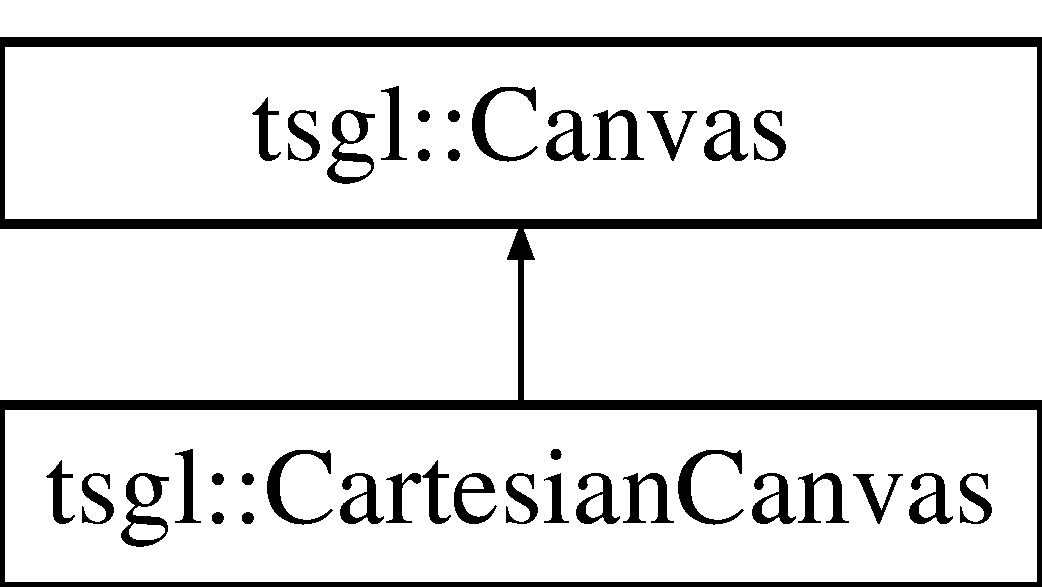
\includegraphics[height=2.000000cm]{classtsgl_1_1_cartesian_canvas}
\end{center}
\end{figure}
\subsection*{\-Public \-Member \-Functions}
\begin{DoxyCompactItemize}
\item 
\hyperlink{classtsgl_1_1_cartesian_canvas_a4438f368eae3def6a70e0faa15d28daa}{\-Cartesian\-Canvas} (double timer\-Length=0.\-0)
\begin{DoxyCompactList}\small\item\em \-Default \hyperlink{classtsgl_1_1_cartesian_canvas}{\-Cartesian\-Canvas} constructor method. \end{DoxyCompactList}\item 
\hyperlink{classtsgl_1_1_cartesian_canvas_a7ca80bfa69d89fdbe110a7ec3aa6f100}{\-Cartesian\-Canvas} (int x, int y, int width, int height, \-Decimal x\-Min, \-Decimal y\-Min, \-Decimal x\-Max, \-Decimal y\-Max, std\-::string t, double timer\-Length=0.\-0)
\begin{DoxyCompactList}\small\item\em \-Explicit \hyperlink{classtsgl_1_1_cartesian_canvas}{\-Cartesian\-Canvas} constructor method. \end{DoxyCompactList}\item 
void \hyperlink{classtsgl_1_1_cartesian_canvas_a1b08e3c0d692603fd2bf56e38eb19907}{draw\-Axes} (\-Decimal origin\-X, \-Decimal origin\-Y, \-Decimal spacing\-X, \-Decimal spacing\-Y)
\begin{DoxyCompactList}\small\item\em \-Draws axes on the \-Cartesian \hyperlink{classtsgl_1_1_canvas}{\-Canvas}. \end{DoxyCompactList}\item 
void \hyperlink{classtsgl_1_1_cartesian_canvas_a64e128195cbcf9b60dbe478d6f489d67}{draw\-Circle} (\-Decimal x, \-Decimal y, \-Decimal radius, int sides, \hyperlink{structtsgl_1_1_color_float}{\-Color\-Float} color=\-B\-L\-A\-C\-K, bool filled=true)
\begin{DoxyCompactList}\small\item\em \-Draws a circle. \end{DoxyCompactList}\item 
void \hyperlink{classtsgl_1_1_cartesian_canvas_a7f84b79ab6fd77277c5c71fce7d0ec6a}{draw\-Concave\-Polygon} (int size, \-Decimal xverts\mbox{[}$\,$\mbox{]}, \-Decimal yverts\mbox{[}$\,$\mbox{]}, \hyperlink{structtsgl_1_1_color_float}{\-Color\-Float} color\mbox{[}$\,$\mbox{]}, bool filled=true)
\begin{DoxyCompactList}\small\item\em \-Draws a \-Concave polygon with colored vertices. \end{DoxyCompactList}\item 
void \hyperlink{classtsgl_1_1_cartesian_canvas_abefc7f373711cdff2477d0665b37212f}{draw\-Convex\-Polygon} (int size, \-Decimal xverts\mbox{[}$\,$\mbox{]}, \-Decimal yverts\mbox{[}$\,$\mbox{]}, \hyperlink{structtsgl_1_1_color_float}{\-Color\-Float} color\mbox{[}$\,$\mbox{]}, bool filled=true)
\begin{DoxyCompactList}\small\item\em \-Draws a convex polygon with colored vertices. \end{DoxyCompactList}\item 
void \hyperlink{classtsgl_1_1_cartesian_canvas_aa8c215b817d95e3e05ff26f835470c41}{draw\-Function} (const \hyperlink{classtsgl_1_1_function}{\-Function} \&function, float sleep\-Time=0.\-0f, Color\-Float color=\-B\-L\-A\-C\-K)
\begin{DoxyCompactList}\small\item\em \-Plots a function on the screen. \end{DoxyCompactList}\item 
void \hyperlink{classtsgl_1_1_cartesian_canvas_acf5536fbf6dca6df1fec719e13630a02}{draw\-Function} (function\-Pointer \&function, float sleep\-Time=0.\-0f, Color\-Float color=\-B\-L\-A\-C\-K)
\begin{DoxyCompactList}\small\item\em \-Plots a function on the screen. \end{DoxyCompactList}\item 
void \hyperlink{classtsgl_1_1_cartesian_canvas_ab2f3e7633f4f05711083eba01b0a3f4e}{draw\-Image} (std\-::string filename, \-Decimal x, \-Decimal y, \-Decimal w, \-Decimal h, float a=1.\-0f)
\begin{DoxyCompactList}\small\item\em \-Draws an image. \end{DoxyCompactList}\item 
void \hyperlink{classtsgl_1_1_cartesian_canvas_ace015a630f1ff280b2ecd6a864cdc5e2}{draw\-Line} (\-Decimal x1, \-Decimal y1, \-Decimal x2, \-Decimal y2, \hyperlink{structtsgl_1_1_color_float}{\-Color\-Float} color=\-B\-L\-A\-C\-K)
\begin{DoxyCompactList}\small\item\em \-Draws a line. \end{DoxyCompactList}\item 
void \hyperlink{classtsgl_1_1_cartesian_canvas_a8b0d9607230111dd6bef5bf270394b03}{draw\-Partial\-Function} (function\-Pointer \&function, \-Decimal min, \-Decimal max, float sleep\-Time=0.\-0f, Color\-Float color=\-B\-L\-A\-C\-K)
\begin{DoxyCompactList}\small\item\em \-Plots part of a function on the screen. \end{DoxyCompactList}\item 
void \hyperlink{classtsgl_1_1_cartesian_canvas_ad0bdf8651a9f703cfd6f71a6bd6ffe17}{draw\-Pixel} (\-Decimal row, \-Decimal col, \hyperlink{structtsgl_1_1_color_float}{\-Color\-Float} color=\-B\-L\-A\-C\-K)
\begin{DoxyCompactList}\small\item\em \-Draws a single pixel, specified in row,column format. \end{DoxyCompactList}\item 
void \hyperlink{classtsgl_1_1_cartesian_canvas_a2ef932501dd03f885fd0ff30ddffae01}{draw\-Point} (\-Decimal x, \-Decimal y, \hyperlink{structtsgl_1_1_color_float}{\-Color\-Float} color=\-B\-L\-A\-C\-K)
\begin{DoxyCompactList}\small\item\em \-Draws a single pixel, specified in x,y format. \end{DoxyCompactList}\item 
void \hyperlink{classtsgl_1_1_cartesian_canvas_a5e88e7d751e24ae78d158f1d8e9faf5e}{draw\-Rectangle} (\-Decimal x1, \-Decimal y1, \-Decimal x2, \-Decimal y2, \hyperlink{structtsgl_1_1_color_float}{\-Color\-Float} color=\-B\-L\-A\-C\-K, bool filled=true)
\begin{DoxyCompactList}\small\item\em \-Draws a rectangle. \end{DoxyCompactList}\item 
void \hyperlink{classtsgl_1_1_cartesian_canvas_a7df01e80ce99d0ce6b45532034c0940c}{draw\-Text} (std\-::string text, \-Decimal x, \-Decimal y, unsigned size, \hyperlink{structtsgl_1_1_color_float}{\-Color\-Float} color=\-B\-L\-A\-C\-K)
\begin{DoxyCompactList}\small\item\em \-Draw a string of text. \end{DoxyCompactList}\item 
void \hyperlink{classtsgl_1_1_cartesian_canvas_addacb4d3637bf2674e2a992a0c165160}{draw\-Text} (std\-::wstring text, \-Decimal x, \-Decimal y, unsigned size, \hyperlink{structtsgl_1_1_color_float}{\-Color\-Float} color=\-B\-L\-A\-C\-K)
\begin{DoxyCompactList}\small\item\em \-Draw a string of text. \end{DoxyCompactList}\item 
void \hyperlink{classtsgl_1_1_cartesian_canvas_a67c225592f9416de476943bb93309cd1}{draw\-Triangle} (\-Decimal x1, \-Decimal y1, \-Decimal x2, \-Decimal y2, \-Decimal x3, \-Decimal y3, \hyperlink{structtsgl_1_1_color_float}{\-Color\-Float} color=\-B\-L\-A\-C\-K, bool filled=true)
\begin{DoxyCompactList}\small\item\em \-Draw a triangle. \end{DoxyCompactList}\item 
void \hyperlink{classtsgl_1_1_cartesian_canvas_a924f6148489c634ec4d47970e498a26a}{draw\-Triangle\-Strip} (int size, \-Decimal xverts\mbox{[}$\,$\mbox{]}, \-Decimal yverts\mbox{[}$\,$\mbox{]}, \hyperlink{structtsgl_1_1_color_float}{\-Color\-Float} color\mbox{[}$\,$\mbox{]}, bool filled=true)
\begin{DoxyCompactList}\small\item\em \-Draws an arbitrary triangle strip with colored vertices. \end{DoxyCompactList}\item 
void \hyperlink{classtsgl_1_1_cartesian_canvas_a736935074bb6d90bcc0c7af2edd8a4aa}{get\-Cartesian\-Coordinates} (int screen\-X, int screen\-Y, \-Decimal \&cart\-X, \-Decimal \&cart\-Y)
\begin{DoxyCompactList}\small\item\em \-Translates \-Cartesian coordinates into window coordinates. \end{DoxyCompactList}\item 
\-Decimal \hyperlink{classtsgl_1_1_cartesian_canvas_a66657636eaf20ff465898d3f932063ce}{get\-Cart\-Height} ()
\begin{DoxyCompactList}\small\item\em \-Accessor for the \hyperlink{classtsgl_1_1_cartesian_canvas}{\-Cartesian\-Canvas}'s \-Cartesian height. \end{DoxyCompactList}\item 
\-Decimal \hyperlink{classtsgl_1_1_cartesian_canvas_a829a97323261515097b7589bc96c109c}{get\-Cart\-Width} ()
\begin{DoxyCompactList}\small\item\em \-Accessor for the \hyperlink{classtsgl_1_1_cartesian_canvas}{\-Cartesian\-Canvas}'s \-Cartesian width. \end{DoxyCompactList}\item 
\-Decimal \hyperlink{classtsgl_1_1_cartesian_canvas_ae3cbac386f78ecff082b8c4cbd9081ed}{get\-Max\-X} ()
\begin{DoxyCompactList}\small\item\em \-Accessor for the \hyperlink{classtsgl_1_1_cartesian_canvas}{\-Cartesian\-Canvas}'s right bound. \end{DoxyCompactList}\item 
\-Decimal \hyperlink{classtsgl_1_1_cartesian_canvas_a68c0616f8180690423d39e9e83045b8c}{get\-Max\-Y} ()
\begin{DoxyCompactList}\small\item\em \-Accessor for the \hyperlink{classtsgl_1_1_cartesian_canvas}{\-Cartesian\-Canvas}'s top bound. \end{DoxyCompactList}\item 
\-Decimal \hyperlink{classtsgl_1_1_cartesian_canvas_a4ab031c60f6fed675e8163c30c01e5d6}{get\-Min\-X} ()
\begin{DoxyCompactList}\small\item\em \-Accessor for the \hyperlink{classtsgl_1_1_cartesian_canvas}{\-Cartesian\-Canvas}'s left bound. \end{DoxyCompactList}\item 
\-Decimal \hyperlink{classtsgl_1_1_cartesian_canvas_a99c935c99c9a29f2cc918963d734d9a6}{get\-Min\-Y} ()
\begin{DoxyCompactList}\small\item\em \-Accessor for the \hyperlink{classtsgl_1_1_cartesian_canvas}{\-Cartesian\-Canvas}'s bottom bound. \end{DoxyCompactList}\item 
\-Decimal \hyperlink{classtsgl_1_1_cartesian_canvas_ac9bb990b8c34a1575bcb861e4b819372}{get\-Pixel\-Width} ()
\begin{DoxyCompactList}\small\item\em \-Accessor for the \hyperlink{classtsgl_1_1_cartesian_canvas}{\-Cartesian\-Canvas}'s effective pixel width. \end{DoxyCompactList}\item 
\-Decimal \hyperlink{classtsgl_1_1_cartesian_canvas_a699c2b41b3b46bfac8649fb38b24c901}{get\-Pixel\-Height} ()
\begin{DoxyCompactList}\small\item\em \-Accessor for the \hyperlink{classtsgl_1_1_cartesian_canvas}{\-Cartesian\-Canvas}'s effective pixel height. \end{DoxyCompactList}\item 
void \hyperlink{classtsgl_1_1_cartesian_canvas_a8fea34cfcee9bc577c1e1ab6d28a8185}{get\-Screen\-Coordinates} (\-Decimal cart\-X, \-Decimal cart\-Y, int \&screen\-X, int \&screen\-Y)
\begin{DoxyCompactList}\small\item\em \-Translates window coordinates into \-Cartesian coordinates. \end{DoxyCompactList}\item 
void \hyperlink{classtsgl_1_1_cartesian_canvas_ac833a44fe7367f6411292707de37beef}{recompute\-Dimensions} (\-Decimal x\-Min, \-Decimal y\-Min, \-Decimal x\-Max, \-Decimal y\-Max)
\begin{DoxyCompactList}\small\item\em \-Recomputes the \hyperlink{classtsgl_1_1_cartesian_canvas}{\-Cartesian\-Canvas}'s bounds. \end{DoxyCompactList}\item 
void \hyperlink{classtsgl_1_1_cartesian_canvas_a63a948af53582b713957b872a765dcdb}{run} (void($\ast$my\-Function)(\hyperlink{classtsgl_1_1_cartesian_canvas}{\-Cartesian\-Canvas} \&))
\begin{DoxyCompactList}\small\item\em \-Start the \hyperlink{classtsgl_1_1_cartesian_canvas}{\-Cartesian\-Canvas}, run a function on it, and wait for the user to close it. \end{DoxyCompactList}\item 
void \hyperlink{classtsgl_1_1_cartesian_canvas_a4d50613e241cab83878aa4438f3db67e}{run} (void($\ast$my\-Function)(\hyperlink{classtsgl_1_1_cartesian_canvas}{\-Cartesian\-Canvas} \&, int), int i)
\begin{DoxyCompactList}\small\item\em \-Overload for \hyperlink{classtsgl_1_1_cartesian_canvas_a63a948af53582b713957b872a765dcdb}{run()} \end{DoxyCompactList}\item 
void \hyperlink{classtsgl_1_1_cartesian_canvas_ab18eee19a5a0c7011c4442b64d05f6cc}{run} (void($\ast$my\-Function)(\hyperlink{classtsgl_1_1_cartesian_canvas}{\-Cartesian\-Canvas} \&, unsigned), unsigned u)
\begin{DoxyCompactList}\small\item\em \-Overload for \hyperlink{classtsgl_1_1_cartesian_canvas_a63a948af53582b713957b872a765dcdb}{run()} \end{DoxyCompactList}\item 
void \hyperlink{classtsgl_1_1_cartesian_canvas_aae4be78e02055eed3e6e85bb39411f21}{run} (void($\ast$my\-Function)(\hyperlink{classtsgl_1_1_cartesian_canvas}{\-Cartesian\-Canvas} \&, int, int), int i1, int i2)
\begin{DoxyCompactList}\small\item\em \-Overload for \hyperlink{classtsgl_1_1_cartesian_canvas_a63a948af53582b713957b872a765dcdb}{run()} \end{DoxyCompactList}\item 
void \hyperlink{classtsgl_1_1_cartesian_canvas_a3351ccc624bb154dc910cafd9effe3cd}{run} (void($\ast$my\-Function)(\hyperlink{classtsgl_1_1_cartesian_canvas}{\-Cartesian\-Canvas} \&, unsigned, unsigned), unsigned u1, unsigned u2)
\begin{DoxyCompactList}\small\item\em \-Overload for \hyperlink{classtsgl_1_1_cartesian_canvas_a63a948af53582b713957b872a765dcdb}{run()} \end{DoxyCompactList}\item 
void \hyperlink{classtsgl_1_1_cartesian_canvas_a7d76ab9f68d8ce7f76b6be20305a5e95}{run} (void($\ast$my\-Function)(\hyperlink{classtsgl_1_1_cartesian_canvas}{\-Cartesian\-Canvas} \&, std\-::string), std\-::string s)
\begin{DoxyCompactList}\small\item\em \-Overload for \hyperlink{classtsgl_1_1_cartesian_canvas_a63a948af53582b713957b872a765dcdb}{run()} \end{DoxyCompactList}\item 
void \hyperlink{classtsgl_1_1_cartesian_canvas_ab0bce76883df5ae48e368a7b7835aefd}{run} (void($\ast$my\-Function)(\hyperlink{classtsgl_1_1_cartesian_canvas}{\-Cartesian\-Canvas} \&, int, std\-::string), int i, std\-::string s)
\begin{DoxyCompactList}\small\item\em \-Overload for \hyperlink{classtsgl_1_1_cartesian_canvas_a63a948af53582b713957b872a765dcdb}{run()} \end{DoxyCompactList}\item 
void \hyperlink{classtsgl_1_1_cartesian_canvas_abf52fc46a6fdca1410db6feb3c67a3cd}{run} (void($\ast$my\-Function)(\hyperlink{classtsgl_1_1_cartesian_canvas}{\-Cartesian\-Canvas} \&, std\-::string, int), std\-::string s, int i)
\begin{DoxyCompactList}\small\item\em \-Overload for \hyperlink{classtsgl_1_1_cartesian_canvas_a63a948af53582b713957b872a765dcdb}{run()} \end{DoxyCompactList}\item 
void \hyperlink{classtsgl_1_1_cartesian_canvas_a3ae99570b9a5f68f4ccf31593867edb0}{sleep} ()
\begin{DoxyCompactList}\small\item\em \-Sleeps the internal drawing timer of a \hyperlink{classtsgl_1_1_cartesian_canvas}{\-Cartesian\-Canvas} object. \end{DoxyCompactList}\item 
void \hyperlink{classtsgl_1_1_cartesian_canvas_a69a378f61868c4c880889c33ec33c992}{zoom} (\-Decimal x, \-Decimal y, \-Decimal scale)
\begin{DoxyCompactList}\small\item\em \-Zoom the \hyperlink{classtsgl_1_1_cartesian_canvas}{\-Cartesian\-Canvas} with a given center. \end{DoxyCompactList}\item 
void \hyperlink{classtsgl_1_1_cartesian_canvas_adb1e999087c0ec7e4405d8ebd3ca9760}{zoom} (\-Decimal x1, \-Decimal y1, \-Decimal x2, \-Decimal y2)
\begin{DoxyCompactList}\small\item\em \-Zoom the \hyperlink{classtsgl_1_1_cartesian_canvas}{\-Cartesian\-Canvas} with the given bounding (\-Cartesian) coordinates. \end{DoxyCompactList}\end{DoxyCompactItemize}
\subsection*{\-Static \-Public \-Member \-Functions}
\begin{DoxyCompactItemize}
\item 
\hypertarget{classtsgl_1_1_cartesian_canvas_ae40d704629167ff70303a3c55ee3bb43}{static void \hyperlink{classtsgl_1_1_cartesian_canvas_ae40d704629167ff70303a3c55ee3bb43}{run\-Tests} ()}\label{classtsgl_1_1_cartesian_canvas_ae40d704629167ff70303a3c55ee3bb43}

\begin{DoxyCompactList}\small\item\em \-Runs the \-Unit tests for \hyperlink{classtsgl_1_1_cartesian_canvas}{\-Cartesian\-Canvas}. \end{DoxyCompactList}\end{DoxyCompactItemize}


\subsection{\-Detailed \-Description}
\hyperlink{classtsgl_1_1_canvas}{\-Canvas} extended with \-Cartesian drawing operations. 

\hyperlink{classtsgl_1_1_cartesian_canvas}{\-Cartesian\-Canvas} provides a \hyperlink{classtsgl_1_1_canvas}{\-Canvas} with a \-Cartesian coordinate system for ease of plotting. \begin{DoxyNote}{\-Note}
\-While on a regular \hyperlink{classtsgl_1_1_canvas}{\-Canvas}, pixels higher on the screen have a lower y-\/value, {\bfseries on a \hyperlink{classtsgl_1_1_cartesian_canvas}{\-Cartesian\-Canvas}, pixels higher on the screen have a higher y-\/value.} 
\end{DoxyNote}


\subsection{\-Constructor \& \-Destructor \-Documentation}
\hypertarget{classtsgl_1_1_cartesian_canvas_a4438f368eae3def6a70e0faa15d28daa}{\index{tsgl\-::\-Cartesian\-Canvas@{tsgl\-::\-Cartesian\-Canvas}!\-Cartesian\-Canvas@{\-Cartesian\-Canvas}}
\index{\-Cartesian\-Canvas@{\-Cartesian\-Canvas}!tsgl::CartesianCanvas@{tsgl\-::\-Cartesian\-Canvas}}
\subsubsection[{\-Cartesian\-Canvas}]{\setlength{\rightskip}{0pt plus 5cm}{\bf tsgl\-::\-Cartesian\-Canvas\-::\-Cartesian\-Canvas} (
\begin{DoxyParamCaption}
\item[{double}]{timer\-Length = {\ttfamily 0.0}}
\end{DoxyParamCaption}
)}}\label{classtsgl_1_1_cartesian_canvas_a4438f368eae3def6a70e0faa15d28daa}


\-Default \hyperlink{classtsgl_1_1_cartesian_canvas}{\-Cartesian\-Canvas} constructor method. 

\-This is the default constructor for the \hyperlink{classtsgl_1_1_cartesian_canvas}{\-Cartesian\-Canvas} class. 
\begin{DoxyParams}{\-Parameters}
{\em timer\-Length} & \-The minimum number of seconds between draw cycles for the \hyperlink{classtsgl_1_1_canvas}{\-Canvas}. \-A value less than or equal to 0 sets it to automatic. \\
\hline
\end{DoxyParams}
\begin{DoxyReturn}{\-Returns}
\-A new \hyperlink{classtsgl_1_1_cartesian_canvas}{\-Cartesian\-Canvas}, stretching from -\/400 to +400 on the x axis and -\/300 to +300 on the y axis, in the middle of the screen with no title. \-The created \hyperlink{classtsgl_1_1_cartesian_canvas}{\-Cartesian\-Canvas} will take up approximately 90\% of the monitor's height, and will have a 4\-:3 aspect ratio. 
\end{DoxyReturn}
\hypertarget{classtsgl_1_1_cartesian_canvas_a7ca80bfa69d89fdbe110a7ec3aa6f100}{\index{tsgl\-::\-Cartesian\-Canvas@{tsgl\-::\-Cartesian\-Canvas}!\-Cartesian\-Canvas@{\-Cartesian\-Canvas}}
\index{\-Cartesian\-Canvas@{\-Cartesian\-Canvas}!tsgl::CartesianCanvas@{tsgl\-::\-Cartesian\-Canvas}}
\subsubsection[{\-Cartesian\-Canvas}]{\setlength{\rightskip}{0pt plus 5cm}{\bf tsgl\-::\-Cartesian\-Canvas\-::\-Cartesian\-Canvas} (
\begin{DoxyParamCaption}
\item[{int}]{x, }
\item[{int}]{y, }
\item[{int}]{width, }
\item[{int}]{height, }
\item[{\-Decimal}]{x\-Min, }
\item[{\-Decimal}]{y\-Min, }
\item[{\-Decimal}]{x\-Max, }
\item[{\-Decimal}]{y\-Max, }
\item[{std\-::string}]{t, }
\item[{double}]{timer\-Length = {\ttfamily 0.0}}
\end{DoxyParamCaption}
)}}\label{classtsgl_1_1_cartesian_canvas_a7ca80bfa69d89fdbe110a7ec3aa6f100}


\-Explicit \hyperlink{classtsgl_1_1_cartesian_canvas}{\-Cartesian\-Canvas} constructor method. 

\-This is an explicit constructor for the \hyperlink{classtsgl_1_1_cartesian_canvas}{\-Cartesian\-Canvas} class. 
\begin{DoxyParams}{\-Parameters}
{\em x} & \-The x position of the \hyperlink{classtsgl_1_1_cartesian_canvas}{\-Cartesian\-Canvas} window. \\
\hline
{\em y} & \-The y position of the \hyperlink{classtsgl_1_1_cartesian_canvas}{\-Cartesian\-Canvas} window. \\
\hline
{\em width} & \-The x dimension of the \hyperlink{classtsgl_1_1_cartesian_canvas}{\-Cartesian\-Canvas} window. \\
\hline
{\em height} & \-The y dimension of the \hyperlink{classtsgl_1_1_cartesian_canvas}{\-Cartesian\-Canvas} window. \\
\hline
{\em x\-Min} & \-The \-Cartesian coordinates of the \hyperlink{classtsgl_1_1_cartesian_canvas}{\-Cartesian\-Canvas}'s left bound. \\
\hline
{\em y\-Min} & \-The \-Cartesian coordinates of the \hyperlink{classtsgl_1_1_cartesian_canvas}{\-Cartesian\-Canvas}'s bottom bound. \\
\hline
{\em x\-Max} & \-The \-Cartesian coordinates of the \hyperlink{classtsgl_1_1_cartesian_canvas}{\-Cartesian\-Canvas}'s right bound. \\
\hline
{\em y\-Max} & \-The \-Cartesian coordinates of the \hyperlink{classtsgl_1_1_cartesian_canvas}{\-Cartesian\-Canvas}'s top bound. \\
\hline
{\em title} & \-The title of the window. \\
\hline
{\em timer\-Length} & \-The minimum number of seconds between draw cycles for the \hyperlink{classtsgl_1_1_canvas}{\-Canvas}. \-A value less than or equal to 0 sets it to automatic. \\
\hline
\end{DoxyParams}
\begin{DoxyReturn}{\-Returns}
\-A new \hyperlink{classtsgl_1_1_cartesian_canvas}{\-Cartesian\-Canvas} with the specified position, dimensions, scaling, title, and timer length. 
\end{DoxyReturn}


\subsection{\-Member \-Function \-Documentation}
\hypertarget{classtsgl_1_1_cartesian_canvas_a1b08e3c0d692603fd2bf56e38eb19907}{\index{tsgl\-::\-Cartesian\-Canvas@{tsgl\-::\-Cartesian\-Canvas}!draw\-Axes@{draw\-Axes}}
\index{draw\-Axes@{draw\-Axes}!tsgl::CartesianCanvas@{tsgl\-::\-Cartesian\-Canvas}}
\subsubsection[{draw\-Axes}]{\setlength{\rightskip}{0pt plus 5cm}void {\bf tsgl\-::\-Cartesian\-Canvas\-::draw\-Axes} (
\begin{DoxyParamCaption}
\item[{\-Decimal}]{origin\-X, }
\item[{\-Decimal}]{origin\-Y, }
\item[{\-Decimal}]{spacing\-X, }
\item[{\-Decimal}]{spacing\-Y}
\end{DoxyParamCaption}
)}}\label{classtsgl_1_1_cartesian_canvas_a1b08e3c0d692603fd2bf56e38eb19907}


\-Draws axes on the \-Cartesian \hyperlink{classtsgl_1_1_canvas}{\-Canvas}. 

\-This function draws axes (with tick marks) on the \hyperlink{classtsgl_1_1_cartesian_canvas}{\-Cartesian\-Canvas}, centered at the given (\-Cartesian) coordinates 
\begin{DoxyParams}{\-Parameters}
{\em origin\-X} & \-The horizontal location of the y-\/axis line. \\
\hline
{\em origin\-Y} & \-The vertical location of the x-\/axis line. \\
\hline
{\em spacing\-X} & \-The distance between marks on the x-\/axis. \\
\hline
{\em spacing\-Y} & \-The distance between marks on the y-\/axis. \\
\hline
\end{DoxyParams}
\hypertarget{classtsgl_1_1_cartesian_canvas_a64e128195cbcf9b60dbe478d6f489d67}{\index{tsgl\-::\-Cartesian\-Canvas@{tsgl\-::\-Cartesian\-Canvas}!draw\-Circle@{draw\-Circle}}
\index{draw\-Circle@{draw\-Circle}!tsgl::CartesianCanvas@{tsgl\-::\-Cartesian\-Canvas}}
\subsubsection[{draw\-Circle}]{\setlength{\rightskip}{0pt plus 5cm}void {\bf tsgl\-::\-Cartesian\-Canvas\-::draw\-Circle} (
\begin{DoxyParamCaption}
\item[{\-Decimal}]{x, }
\item[{\-Decimal}]{y, }
\item[{\-Decimal}]{radius, }
\item[{int}]{sides, }
\item[{{\bf \-Color\-Float}}]{color = {\ttfamily \-B\-L\-A\-C\-K}, }
\item[{bool}]{filled = {\ttfamily true}}
\end{DoxyParamCaption}
)}}\label{classtsgl_1_1_cartesian_canvas_a64e128195cbcf9b60dbe478d6f489d67}


\-Draws a circle. 

\-This function draws a circle with the given center, radius, resolution (number of sides), color, and fill status. 
\begin{DoxyParams}{\-Parameters}
{\em x} & \-The x coordinate of the circle's center. \\
\hline
{\em y} & \-The y coordinate of the circle's center. \\
\hline
{\em radius} & \-The radius of the circle in pixels. \\
\hline
{\em sides} & \-The number of sides to use in the circle. \\
\hline
{\em color} & \-The color of the circle (set to \-B\-L\-A\-C\-K by default). \\
\hline
{\em filled} & \-Whether the circle should be filled (set to true by default). \\
\hline
\end{DoxyParams}
\begin{DoxyNote}{\-Note}
\-Identical to \hyperlink{classtsgl_1_1_canvas_a2162c16f6aeaee01f8e29696f5818c03}{\-Canvas\-::draw\-Circle()}. 
\end{DoxyNote}
\hypertarget{classtsgl_1_1_cartesian_canvas_a7f84b79ab6fd77277c5c71fce7d0ec6a}{\index{tsgl\-::\-Cartesian\-Canvas@{tsgl\-::\-Cartesian\-Canvas}!draw\-Concave\-Polygon@{draw\-Concave\-Polygon}}
\index{draw\-Concave\-Polygon@{draw\-Concave\-Polygon}!tsgl::CartesianCanvas@{tsgl\-::\-Cartesian\-Canvas}}
\subsubsection[{draw\-Concave\-Polygon}]{\setlength{\rightskip}{0pt plus 5cm}void {\bf tsgl\-::\-Cartesian\-Canvas\-::draw\-Concave\-Polygon} (
\begin{DoxyParamCaption}
\item[{int}]{size, }
\item[{\-Decimal}]{xverts\mbox{[}$\,$\mbox{]}, }
\item[{\-Decimal}]{yverts\mbox{[}$\,$\mbox{]}, }
\item[{{\bf \-Color\-Float}}]{color\mbox{[}$\,$\mbox{]}, }
\item[{bool}]{filled = {\ttfamily true}}
\end{DoxyParamCaption}
)}}\label{classtsgl_1_1_cartesian_canvas_a7f84b79ab6fd77277c5c71fce7d0ec6a}


\-Draws a \-Concave polygon with colored vertices. 

\-This function draws a \hyperlink{classtsgl_1_1_concave_polygon}{\-Concave\-Polygon} with the given vertex data, specified as the outer perimeter of the polygon. 
\begin{DoxyParams}{\-Parameters}
{\em size} & \-The number of vertices in the polygon. \\
\hline
{\em xverts} & \-An array of x positions of said vertices. \\
\hline
{\em yverts} & \-An array of y positions of said vertices. \\
\hline
{\em color} & \-An array of colors for the said vertices. \\
\hline
{\em filled} & \-Whether the \-Concave polygon should be filled in or not (set to true by default). \\
\hline
\end{DoxyParams}
\begin{DoxyWarning}{\-Warning}
{\bfseries \-This function is significantly slower than \hyperlink{classtsgl_1_1_cartesian_canvas_abefc7f373711cdff2477d0665b37212f}{draw\-Convex\-Polygon()}. \-It is not recommended that you draw \-Convex polygons with this function. }
\end{DoxyWarning}
\begin{DoxyNote}{\-Note}
{\bfseries  \-Identical to \hyperlink{classtsgl_1_1_canvas_ad98cb8db661ef24279b61c4c11fd29ea}{\-Canvas\-::draw\-Concave\-Polygon()}. }
\end{DoxyNote}
\begin{DoxySeeAlso}{\-See also}
{\bfseries  \hyperlink{classtsgl_1_1_cartesian_canvas_abefc7f373711cdff2477d0665b37212f}{draw\-Convex\-Polygon()}. }
\end{DoxySeeAlso}
\hypertarget{classtsgl_1_1_cartesian_canvas_abefc7f373711cdff2477d0665b37212f}{\index{tsgl\-::\-Cartesian\-Canvas@{tsgl\-::\-Cartesian\-Canvas}!draw\-Convex\-Polygon@{draw\-Convex\-Polygon}}
\index{draw\-Convex\-Polygon@{draw\-Convex\-Polygon}!tsgl::CartesianCanvas@{tsgl\-::\-Cartesian\-Canvas}}
\subsubsection[{draw\-Convex\-Polygon}]{\setlength{\rightskip}{0pt plus 5cm}void {\bf tsgl\-::\-Cartesian\-Canvas\-::draw\-Convex\-Polygon} (
\begin{DoxyParamCaption}
\item[{int}]{size, }
\item[{\-Decimal}]{xverts\mbox{[}$\,$\mbox{]}, }
\item[{\-Decimal}]{yverts\mbox{[}$\,$\mbox{]}, }
\item[{{\bf \-Color\-Float}}]{color\mbox{[}$\,$\mbox{]}, }
\item[{bool}]{filled = {\ttfamily true}}
\end{DoxyParamCaption}
)}}\label{classtsgl_1_1_cartesian_canvas_abefc7f373711cdff2477d0665b37212f}


\-Draws a convex polygon with colored vertices. 

\-This function draws a \hyperlink{classtsgl_1_1_convex_polygon}{\-Convex\-Polygon} with the given vertex data, specified as the outer perimeter of the polygon. 
\begin{DoxyParams}{\-Parameters}
{\em size} & \-The number of vertices in the polygon. \\
\hline
{\em xverts} & \-An array of the x positions of said vertices. \\
\hline
{\em yverts} & \-An array of the y positions of said vertices. \\
\hline
{\em color} & \-An array of colors for the said vertices. \\
\hline
{\em filled} & \-Whether the \hyperlink{classtsgl_1_1_convex_polygon}{\-Convex\-Polygon} should be filled in or not (set to true by default). \\
\hline
\end{DoxyParams}
\begin{DoxyNote}{\-Note}
\-The difference between a convex polygon and a concave polygon is that a convex polygon has all interior angles less than 180 degrees ( see \href{http://www.mathopenref.com/polygonconvex.html}{\tt http\-://www.\-mathopenref.\-com/polygonconvex.\-html} ). 

\-Identical to \hyperlink{classtsgl_1_1_canvas_a9cb84248c3559c81e4cb2e0d194b2437}{\-Canvas\-::draw\-Convex\-Polygon()}. 
\end{DoxyNote}


\-Referenced by tsgl\-::\-Integral\-Viewer\-::trapezoid\-Evaluate().

\hypertarget{classtsgl_1_1_cartesian_canvas_aa8c215b817d95e3e05ff26f835470c41}{\index{tsgl\-::\-Cartesian\-Canvas@{tsgl\-::\-Cartesian\-Canvas}!draw\-Function@{draw\-Function}}
\index{draw\-Function@{draw\-Function}!tsgl::CartesianCanvas@{tsgl\-::\-Cartesian\-Canvas}}
\subsubsection[{draw\-Function}]{\setlength{\rightskip}{0pt plus 5cm}void {\bf tsgl\-::\-Cartesian\-Canvas\-::draw\-Function} (
\begin{DoxyParamCaption}
\item[{const {\bf \-Function} \&}]{function, }
\item[{float}]{sleep\-Time = {\ttfamily 0.0f}, }
\item[{{\bf \-Color\-Float}}]{color = {\ttfamily \-B\-L\-A\-C\-K}}
\end{DoxyParamCaption}
)}}\label{classtsgl_1_1_cartesian_canvas_aa8c215b817d95e3e05ff26f835470c41}


\-Plots a function on the screen. 

\-This function receives a \-T\-S\-G\-L \hyperlink{classtsgl_1_1_function}{\-Function} instance as a parameter and plots the function on the \hyperlink{classtsgl_1_1_cartesian_canvas}{\-Cartesian\-Canvas}. 
\begin{DoxyParams}{\-Parameters}
{\em function} & \-Reference to the \hyperlink{classtsgl_1_1_function}{\-Function} to plot. \\
\hline
{\em sleep\-Time} & \-Time to sleep between plotting points \\
\hline
{\em color} & \-The color of the vertices of the plotted function (set to \-B\-L\-A\-C\-K by default). \\
\hline
\end{DoxyParams}
\hypertarget{classtsgl_1_1_cartesian_canvas_acf5536fbf6dca6df1fec719e13630a02}{\index{tsgl\-::\-Cartesian\-Canvas@{tsgl\-::\-Cartesian\-Canvas}!draw\-Function@{draw\-Function}}
\index{draw\-Function@{draw\-Function}!tsgl::CartesianCanvas@{tsgl\-::\-Cartesian\-Canvas}}
\subsubsection[{draw\-Function}]{\setlength{\rightskip}{0pt plus 5cm}void {\bf tsgl\-::\-Cartesian\-Canvas\-::draw\-Function} (
\begin{DoxyParamCaption}
\item[{function\-Pointer \&}]{function, }
\item[{float}]{sleep\-Time = {\ttfamily 0.0f}, }
\item[{{\bf \-Color\-Float}}]{color = {\ttfamily \-B\-L\-A\-C\-K}}
\end{DoxyParamCaption}
)}}\label{classtsgl_1_1_cartesian_canvas_acf5536fbf6dca6df1fec719e13630a02}


\-Plots a function on the screen. 

\-This function receives a pointer to a function method as a parameter and plots the function on the \hyperlink{classtsgl_1_1_cartesian_canvas}{\-Cartesian\-Canvas}. 
\begin{DoxyParams}{\-Parameters}
{\em function} & \-Pointer to the function-\/drawing method to plot. \\
\hline
{\em sleep\-Time} & \-Time to sleep between plotting points \\
\hline
{\em color} & \-The color of the vertices of the plotted function (set to \-B\-L\-A\-C\-K by default). \\
\hline
\end{DoxyParams}
\begin{DoxyNote}{\-Note}
{\ttfamily function} must receive exactly one \-Decimal x parameter, and return a \-Decimal y parameter. 
\end{DoxyNote}
\hypertarget{classtsgl_1_1_cartesian_canvas_ab2f3e7633f4f05711083eba01b0a3f4e}{\index{tsgl\-::\-Cartesian\-Canvas@{tsgl\-::\-Cartesian\-Canvas}!draw\-Image@{draw\-Image}}
\index{draw\-Image@{draw\-Image}!tsgl::CartesianCanvas@{tsgl\-::\-Cartesian\-Canvas}}
\subsubsection[{draw\-Image}]{\setlength{\rightskip}{0pt plus 5cm}void {\bf tsgl\-::\-Cartesian\-Canvas\-::draw\-Image} (
\begin{DoxyParamCaption}
\item[{std\-::string}]{filename, }
\item[{\-Decimal}]{x, }
\item[{\-Decimal}]{y, }
\item[{\-Decimal}]{w, }
\item[{\-Decimal}]{h, }
\item[{float}]{a = {\ttfamily 1.0f}}
\end{DoxyParamCaption}
)}}\label{classtsgl_1_1_cartesian_canvas_ab2f3e7633f4f05711083eba01b0a3f4e}


\-Draws an image. 

\-This function draws an \hyperlink{classtsgl_1_1_image}{\-Image} with the given coordinates and dimensions. 
\begin{DoxyParams}{\-Parameters}
{\em function} & \-The name of the file to load the image from. \\
\hline
{\em x} & \-The x coordinate of the \hyperlink{classtsgl_1_1_image}{\-Image}'s left edge. \\
\hline
{\em y} & \-The y coordinate of the \hyperlink{classtsgl_1_1_image}{\-Image}'s top edge. \\
\hline
{\em w} & \-The width of the \hyperlink{classtsgl_1_1_image}{\-Image}. \\
\hline
{\em h} & \-The height of the \hyperlink{classtsgl_1_1_image}{\-Image}. \\
\hline
{\em a} & \-The alpha with which to draw the \hyperlink{classtsgl_1_1_image}{\-Image} (set to 1.\-0f by default). \\
\hline
\end{DoxyParams}
\begin{DoxyNote}{\-Note}
\-Identical to \hyperlink{classtsgl_1_1_canvas_ae94a586629d20b7fabcb402d1c654628}{\-Canvas\-::draw\-Image()}. 
\end{DoxyNote}
\hypertarget{classtsgl_1_1_cartesian_canvas_ace015a630f1ff280b2ecd6a864cdc5e2}{\index{tsgl\-::\-Cartesian\-Canvas@{tsgl\-::\-Cartesian\-Canvas}!draw\-Line@{draw\-Line}}
\index{draw\-Line@{draw\-Line}!tsgl::CartesianCanvas@{tsgl\-::\-Cartesian\-Canvas}}
\subsubsection[{draw\-Line}]{\setlength{\rightskip}{0pt plus 5cm}void {\bf tsgl\-::\-Cartesian\-Canvas\-::draw\-Line} (
\begin{DoxyParamCaption}
\item[{\-Decimal}]{x1, }
\item[{\-Decimal}]{y1, }
\item[{\-Decimal}]{x2, }
\item[{\-Decimal}]{y2, }
\item[{{\bf \-Color\-Float}}]{color = {\ttfamily \-B\-L\-A\-C\-K}}
\end{DoxyParamCaption}
)}}\label{classtsgl_1_1_cartesian_canvas_ace015a630f1ff280b2ecd6a864cdc5e2}


\-Draws a line. 

\-This function draws a \hyperlink{classtsgl_1_1_line}{\-Line} at the given coordinates with the given color. 
\begin{DoxyParams}{\-Parameters}
{\em x1} & \-The x position of the start of the line. \\
\hline
{\em y1} & \-The y position of the start of the line. \\
\hline
{\em x2} & \-The x position of the end of the line. \\
\hline
{\em y2} & \-The y position of the end of the line. \\
\hline
{\em color} & \-The color of the line (set to \-B\-L\-A\-C\-K by default). \\
\hline
\end{DoxyParams}
\begin{DoxyNote}{\-Note}
\-Identical to \hyperlink{classtsgl_1_1_canvas_a6e5c605b03a69e615fe4ccee30be1959}{\-Canvas\-::draw\-Line()}. 
\end{DoxyNote}


\-Referenced by draw\-Axes(), draw\-Function(), and draw\-Partial\-Function().

\hypertarget{classtsgl_1_1_cartesian_canvas_a8b0d9607230111dd6bef5bf270394b03}{\index{tsgl\-::\-Cartesian\-Canvas@{tsgl\-::\-Cartesian\-Canvas}!draw\-Partial\-Function@{draw\-Partial\-Function}}
\index{draw\-Partial\-Function@{draw\-Partial\-Function}!tsgl::CartesianCanvas@{tsgl\-::\-Cartesian\-Canvas}}
\subsubsection[{draw\-Partial\-Function}]{\setlength{\rightskip}{0pt plus 5cm}void {\bf tsgl\-::\-Cartesian\-Canvas\-::draw\-Partial\-Function} (
\begin{DoxyParamCaption}
\item[{function\-Pointer \&}]{function, }
\item[{\-Decimal}]{min, }
\item[{\-Decimal}]{max, }
\item[{float}]{sleep\-Time = {\ttfamily 0.0f}, }
\item[{{\bf \-Color\-Float}}]{color = {\ttfamily \-B\-L\-A\-C\-K}}
\end{DoxyParamCaption}
)}}\label{classtsgl_1_1_cartesian_canvas_a8b0d9607230111dd6bef5bf270394b03}


\-Plots part of a function on the screen. 

\-This function receives a pointer to a function method as a parameter and plots the function on the \hyperlink{classtsgl_1_1_cartesian_canvas}{\-Cartesian\-Canvas} between the specified minimum and maximum coordinates. 
\begin{DoxyParams}{\-Parameters}
{\em function} & \-Pointer to the function-\/drawing method to plot. \\
\hline
{\em min} & \-Minimum x value to evaluate and plot \\
\hline
{\em max} & \-Maximum x value to evaluate and plot \\
\hline
{\em sleep\-Time} & \-Time to sleep between plotting points \\
\hline
{\em color} & \-The color of the vertices of the plotted function (set to \-B\-L\-A\-C\-K by default). \\
\hline
\end{DoxyParams}
\begin{DoxyNote}{\-Note}
{\ttfamily function} must receive exactly one \-Decimal x parameter, and return a \-Decimal y parameter. 
\end{DoxyNote}


\-Referenced by draw\-Function().

\hypertarget{classtsgl_1_1_cartesian_canvas_ad0bdf8651a9f703cfd6f71a6bd6ffe17}{\index{tsgl\-::\-Cartesian\-Canvas@{tsgl\-::\-Cartesian\-Canvas}!draw\-Pixel@{draw\-Pixel}}
\index{draw\-Pixel@{draw\-Pixel}!tsgl::CartesianCanvas@{tsgl\-::\-Cartesian\-Canvas}}
\subsubsection[{draw\-Pixel}]{\setlength{\rightskip}{0pt plus 5cm}void {\bf tsgl\-::\-Cartesian\-Canvas\-::draw\-Pixel} (
\begin{DoxyParamCaption}
\item[{\-Decimal}]{row, }
\item[{\-Decimal}]{col, }
\item[{{\bf \-Color\-Float}}]{color = {\ttfamily \-B\-L\-A\-C\-K}}
\end{DoxyParamCaption}
)}}\label{classtsgl_1_1_cartesian_canvas_ad0bdf8651a9f703cfd6f71a6bd6ffe17}


\-Draws a single pixel, specified in row,column format. 

\-This function draws a pixel at the given screen coordinates with the given color. \begin{DoxyNote}{\-Note}
(0,0) signifies the {\bfseries top-\/left} of the screen when working with a \hyperlink{classtsgl_1_1_canvas}{\-Canvas} object. 

(0,0) signifies the {\bfseries bottom-\/left} of the screen when working with a \hyperlink{classtsgl_1_1_cartesian_canvas}{\-Cartesian\-Canvas} object. 
\end{DoxyNote}

\begin{DoxyParams}{\-Parameters}
{\em row} & \-The row (y-\/position) of the pixel. \\
\hline
{\em col} & \-The column (x-\/position) of the pixel. \\
\hline
{\em color} & \-The color of the point (set to \-B\-L\-A\-C\-K by default). \\
\hline
\end{DoxyParams}
\begin{DoxySeeAlso}{\-See also}
\hyperlink{classtsgl_1_1_cartesian_canvas_ad0bdf8651a9f703cfd6f71a6bd6ffe17}{draw\-Pixel()} 
\end{DoxySeeAlso}
\begin{DoxyNote}{\-Note}
\-Identical to \hyperlink{classtsgl_1_1_canvas_af17d456eca4ad5a55842f2cf02f48a97}{\-Canvas\-::draw\-Pixel()}. 
\end{DoxyNote}
\hypertarget{classtsgl_1_1_cartesian_canvas_a2ef932501dd03f885fd0ff30ddffae01}{\index{tsgl\-::\-Cartesian\-Canvas@{tsgl\-::\-Cartesian\-Canvas}!draw\-Point@{draw\-Point}}
\index{draw\-Point@{draw\-Point}!tsgl::CartesianCanvas@{tsgl\-::\-Cartesian\-Canvas}}
\subsubsection[{draw\-Point}]{\setlength{\rightskip}{0pt plus 5cm}void {\bf tsgl\-::\-Cartesian\-Canvas\-::draw\-Point} (
\begin{DoxyParamCaption}
\item[{\-Decimal}]{x, }
\item[{\-Decimal}]{y, }
\item[{{\bf \-Color\-Float}}]{color = {\ttfamily \-B\-L\-A\-C\-K}}
\end{DoxyParamCaption}
)}}\label{classtsgl_1_1_cartesian_canvas_a2ef932501dd03f885fd0ff30ddffae01}


\-Draws a single pixel, specified in x,y format. 

\-This function draws a pixel at the given \-Cartesian coordinates with the given color. \begin{DoxyNote}{\-Note}
(0,0) signifies the {\bfseries left-\/top} of the screen when working with a \hyperlink{classtsgl_1_1_canvas}{\-Canvas} object. 

(0,0) signifies the {\bfseries left-\/bottom} of the screen when working with a \hyperlink{classtsgl_1_1_cartesian_canvas}{\-Cartesian\-Canvas} object. 
\end{DoxyNote}

\begin{DoxyParams}{\-Parameters}
{\em x} & \-The x position of the point. \\
\hline
{\em y} & \-The y position of the point. \\
\hline
{\em color} & \-The color of the point (set to \-B\-L\-A\-C\-K by default). \\
\hline
\end{DoxyParams}
\begin{DoxySeeAlso}{\-See also}
\hyperlink{classtsgl_1_1_cartesian_canvas_a2ef932501dd03f885fd0ff30ddffae01}{draw\-Point()} 
\end{DoxySeeAlso}
\begin{DoxyNote}{\-Note}
\-Identical to \hyperlink{classtsgl_1_1_canvas_a6c17c90cd13f7b0184a25e4acc2b7426}{\-Canvas\-::draw\-Point()}. 
\end{DoxyNote}


\-Referenced by draw\-Pixel().

\hypertarget{classtsgl_1_1_cartesian_canvas_a5e88e7d751e24ae78d158f1d8e9faf5e}{\index{tsgl\-::\-Cartesian\-Canvas@{tsgl\-::\-Cartesian\-Canvas}!draw\-Rectangle@{draw\-Rectangle}}
\index{draw\-Rectangle@{draw\-Rectangle}!tsgl::CartesianCanvas@{tsgl\-::\-Cartesian\-Canvas}}
\subsubsection[{draw\-Rectangle}]{\setlength{\rightskip}{0pt plus 5cm}void {\bf tsgl\-::\-Cartesian\-Canvas\-::draw\-Rectangle} (
\begin{DoxyParamCaption}
\item[{\-Decimal}]{x1, }
\item[{\-Decimal}]{y1, }
\item[{\-Decimal}]{x2, }
\item[{\-Decimal}]{y2, }
\item[{{\bf \-Color\-Float}}]{color = {\ttfamily \-B\-L\-A\-C\-K}, }
\item[{bool}]{filled = {\ttfamily true}}
\end{DoxyParamCaption}
)}}\label{classtsgl_1_1_cartesian_canvas_a5e88e7d751e24ae78d158f1d8e9faf5e}


\-Draws a rectangle. 

\-This function draws a \hyperlink{classtsgl_1_1_rectangle}{\-Rectangle} with the given coordinates, dimensions, and color. 
\begin{DoxyParams}{\-Parameters}
{\em x1} & \-The x coordinate of the \hyperlink{classtsgl_1_1_rectangle}{\-Rectangle}'s left edge. \\
\hline
{\em y1} & \-The y coordinate of the \hyperlink{classtsgl_1_1_rectangle}{\-Rectangle}'s top edge. \\
\hline
{\em x2} & \-The x coordinate of the \hyperlink{classtsgl_1_1_rectangle}{\-Rectangle}'s right edge. \\
\hline
{\em y2} & \-The y coordinate of the \hyperlink{classtsgl_1_1_rectangle}{\-Rectangle}'s bottom edge. \\
\hline
{\em color} & \-The color of the rectangle (set to \-B\-L\-A\-C\-K by default). \\
\hline
{\em filled} & \-Whether the rectangle should be filled (set to true by default). \\
\hline
\end{DoxyParams}
\begin{DoxyNote}{\-Note}
\-Identical to \hyperlink{classtsgl_1_1_canvas_a752754cd16d14447cb5e5b0438bebf16}{\-Canvas\-::draw\-Rectangle()}. 
\end{DoxyNote}


\-Referenced by tsgl\-::\-Integral\-Viewer\-::rectangle\-Evaluate().

\hypertarget{classtsgl_1_1_cartesian_canvas_a7df01e80ce99d0ce6b45532034c0940c}{\index{tsgl\-::\-Cartesian\-Canvas@{tsgl\-::\-Cartesian\-Canvas}!draw\-Text@{draw\-Text}}
\index{draw\-Text@{draw\-Text}!tsgl::CartesianCanvas@{tsgl\-::\-Cartesian\-Canvas}}
\subsubsection[{draw\-Text}]{\setlength{\rightskip}{0pt plus 5cm}void {\bf tsgl\-::\-Cartesian\-Canvas\-::draw\-Text} (
\begin{DoxyParamCaption}
\item[{std\-::string}]{text, }
\item[{\-Decimal}]{x, }
\item[{\-Decimal}]{y, }
\item[{unsigned}]{size, }
\item[{{\bf \-Color\-Float}}]{color = {\ttfamily \-B\-L\-A\-C\-K}}
\end{DoxyParamCaption}
)}}\label{classtsgl_1_1_cartesian_canvas_a7df01e80ce99d0ce6b45532034c0940c}


\-Draw a string of text. 

\-This function draws a given string of \hyperlink{classtsgl_1_1_text}{\-Text} at the given coordinates with the given color.  \-The string to draw. 
\begin{DoxyParams}{\-Parameters}
{\em x} & \-The x coordinate of the text's left bound. \\
\hline
{\em y} & \-The y coordinate of the text's left bound. \\
\hline
{\em size} & \-The size of the text in pixels. \\
\hline
{\em color} & \-The color of the \hyperlink{classtsgl_1_1_text}{\-Text} (set to \-B\-L\-A\-C\-K by default). \\
\hline
\end{DoxyParams}
\begin{DoxyNote}{\-Note}
\-Identical to \hyperlink{classtsgl_1_1_canvas_a3457e7ebd17fa5003025ff6bcaaeedf6}{\-Canvas\-::draw\-Text}(std\-::string,..). 
\end{DoxyNote}


\-Referenced by draw\-Text().

\hypertarget{classtsgl_1_1_cartesian_canvas_addacb4d3637bf2674e2a992a0c165160}{\index{tsgl\-::\-Cartesian\-Canvas@{tsgl\-::\-Cartesian\-Canvas}!draw\-Text@{draw\-Text}}
\index{draw\-Text@{draw\-Text}!tsgl::CartesianCanvas@{tsgl\-::\-Cartesian\-Canvas}}
\subsubsection[{draw\-Text}]{\setlength{\rightskip}{0pt plus 5cm}void {\bf tsgl\-::\-Cartesian\-Canvas\-::draw\-Text} (
\begin{DoxyParamCaption}
\item[{std\-::wstring}]{text, }
\item[{\-Decimal}]{x, }
\item[{\-Decimal}]{y, }
\item[{unsigned}]{size, }
\item[{{\bf \-Color\-Float}}]{color = {\ttfamily \-B\-L\-A\-C\-K}}
\end{DoxyParamCaption}
)}}\label{classtsgl_1_1_cartesian_canvas_addacb4d3637bf2674e2a992a0c165160}


\-Draw a string of text. 

\-This function draws a given string of \hyperlink{classtsgl_1_1_text}{\-Text} at the given coordinates with the given color. 
\begin{DoxyParams}{\-Parameters}
{\em text} & \-The \-U\-T\-F8-\/encoded string to draw. \\
\hline
{\em x} & \-The x coordinate of the text's left bound. \\
\hline
{\em y} & \-The y coordinate of the text's left bound. \\
\hline
{\em size} & \-The size of the text in pixels. \\
\hline
{\em color} & \-The color of the \hyperlink{classtsgl_1_1_text}{\-Text} (set to \-B\-L\-A\-C\-K by default). \\
\hline
\end{DoxyParams}
\begin{DoxyNote}{\-Note}
\-Identical to \hyperlink{classtsgl_1_1_canvas_a3457e7ebd17fa5003025ff6bcaaeedf6}{\-Canvas\-::draw\-Text}(std\-::wstring,..). 
\end{DoxyNote}
\hypertarget{classtsgl_1_1_cartesian_canvas_a67c225592f9416de476943bb93309cd1}{\index{tsgl\-::\-Cartesian\-Canvas@{tsgl\-::\-Cartesian\-Canvas}!draw\-Triangle@{draw\-Triangle}}
\index{draw\-Triangle@{draw\-Triangle}!tsgl::CartesianCanvas@{tsgl\-::\-Cartesian\-Canvas}}
\subsubsection[{draw\-Triangle}]{\setlength{\rightskip}{0pt plus 5cm}void {\bf tsgl\-::\-Cartesian\-Canvas\-::draw\-Triangle} (
\begin{DoxyParamCaption}
\item[{\-Decimal}]{x1, }
\item[{\-Decimal}]{y1, }
\item[{\-Decimal}]{x2, }
\item[{\-Decimal}]{y2, }
\item[{\-Decimal}]{x3, }
\item[{\-Decimal}]{y3, }
\item[{{\bf \-Color\-Float}}]{color = {\ttfamily \-B\-L\-A\-C\-K}, }
\item[{bool}]{filled = {\ttfamily true}}
\end{DoxyParamCaption}
)}}\label{classtsgl_1_1_cartesian_canvas_a67c225592f9416de476943bb93309cd1}


\-Draw a triangle. 

\-This function draws a \hyperlink{classtsgl_1_1_triangle}{\-Triangle} with the given vertices. 
\begin{DoxyParams}{\-Parameters}
{\em x1} & \-The x coordinate of the first vertex of the \hyperlink{classtsgl_1_1_triangle}{\-Triangle}. \\
\hline
{\em y1} & \-The y coordinate of the first vertex of the \hyperlink{classtsgl_1_1_triangle}{\-Triangle}. \\
\hline
{\em x2} & \-The x coordinate of the second vertex of the \hyperlink{classtsgl_1_1_triangle}{\-Triangle}. \\
\hline
{\em y2} & \-The y coordinate of the second vertex of the \hyperlink{classtsgl_1_1_triangle}{\-Triangle}. \\
\hline
{\em x3} & \-The x coordinate of the third vertex of the \hyperlink{classtsgl_1_1_triangle}{\-Triangle}. \\
\hline
{\em y3} & \-The y coordinate of the third vertex of the \hyperlink{classtsgl_1_1_triangle}{\-Triangle}. \\
\hline
{\em color} & \-The color of the \hyperlink{classtsgl_1_1_triangle}{\-Triangle} (set to \-B\-L\-A\-C\-K by default). \\
\hline
{\em filled} & \-Whether the \hyperlink{classtsgl_1_1_triangle}{\-Triangle} should be filled (set to true by default). \\
\hline
\end{DoxyParams}
\begin{DoxyNote}{\-Note}
\-Identical to \hyperlink{classtsgl_1_1_canvas_a8abc9ed7d3c55c5d701009040c65000e}{\-Canvas\-::draw\-Triangle()}. 
\end{DoxyNote}
\hypertarget{classtsgl_1_1_cartesian_canvas_a924f6148489c634ec4d47970e498a26a}{\index{tsgl\-::\-Cartesian\-Canvas@{tsgl\-::\-Cartesian\-Canvas}!draw\-Triangle\-Strip@{draw\-Triangle\-Strip}}
\index{draw\-Triangle\-Strip@{draw\-Triangle\-Strip}!tsgl::CartesianCanvas@{tsgl\-::\-Cartesian\-Canvas}}
\subsubsection[{draw\-Triangle\-Strip}]{\setlength{\rightskip}{0pt plus 5cm}void {\bf tsgl\-::\-Cartesian\-Canvas\-::draw\-Triangle\-Strip} (
\begin{DoxyParamCaption}
\item[{int}]{size, }
\item[{\-Decimal}]{xverts\mbox{[}$\,$\mbox{]}, }
\item[{\-Decimal}]{yverts\mbox{[}$\,$\mbox{]}, }
\item[{{\bf \-Color\-Float}}]{color\mbox{[}$\,$\mbox{]}, }
\item[{bool}]{filled = {\ttfamily true}}
\end{DoxyParamCaption}
)}}\label{classtsgl_1_1_cartesian_canvas_a924f6148489c634ec4d47970e498a26a}


\-Draws an arbitrary triangle strip with colored vertices. 

\-This function draws a \hyperlink{classtsgl_1_1_triangle_strip}{\-Triangle\-Strip} with the given vertex data, specified as a triangle strip. 
\begin{DoxyParams}{\-Parameters}
{\em size} & \-The number of vertices in the polygon. \\
\hline
{\em xverts} & \-An array of x positions of the vertices. \\
\hline
{\em yverts} & \-An array of y positions of the vertices. \\
\hline
{\em color} & \-An array of colors for the vertices. \\
\hline
{\em filled} & \-Whether the triangle strip should be filled (true) or not (false) (set to true by default). \\
\hline
\end{DoxyParams}
\begin{DoxyNote}{\-Note}
\-Identical to \hyperlink{classtsgl_1_1_canvas_a8f570c258a8900178190ec15ac074a57}{\-Canvas\-::draw\-Triangle\-Strip()}. 
\end{DoxyNote}
\hypertarget{classtsgl_1_1_cartesian_canvas_a736935074bb6d90bcc0c7af2edd8a4aa}{\index{tsgl\-::\-Cartesian\-Canvas@{tsgl\-::\-Cartesian\-Canvas}!get\-Cartesian\-Coordinates@{get\-Cartesian\-Coordinates}}
\index{get\-Cartesian\-Coordinates@{get\-Cartesian\-Coordinates}!tsgl::CartesianCanvas@{tsgl\-::\-Cartesian\-Canvas}}
\subsubsection[{get\-Cartesian\-Coordinates}]{\setlength{\rightskip}{0pt plus 5cm}void {\bf tsgl\-::\-Cartesian\-Canvas\-::get\-Cartesian\-Coordinates} (
\begin{DoxyParamCaption}
\item[{int}]{screen\-X, }
\item[{int}]{screen\-Y, }
\item[{\-Decimal \&}]{cart\-X, }
\item[{\-Decimal \&}]{cart\-Y}
\end{DoxyParamCaption}
)}}\label{classtsgl_1_1_cartesian_canvas_a736935074bb6d90bcc0c7af2edd8a4aa}


\-Translates \-Cartesian coordinates into window coordinates. 

\hyperlink{classtsgl_1_1_cartesian_canvas_a736935074bb6d90bcc0c7af2edd8a4aa}{get\-Cartesian\-Coordinates()} takes a pair of on-\/screen coordinates and translates them to \-Cartesian coordinates. 
\begin{DoxyParams}{\-Parameters}
{\em screen\-X} & \-The window's x coordinate. \\
\hline
{\em screen\-Y} & \-The window's y coordinate. \\
\hline
{\em cart\-X} & \-A reference variable to be filled with screen\-X's \-Cartesian position. \\
\hline
{\em cart\-Y} & \-A reference variable to be filled with screen\-Y's \-Cartesian position. \\
\hline
\end{DoxyParams}
\hypertarget{classtsgl_1_1_cartesian_canvas_a66657636eaf20ff465898d3f932063ce}{\index{tsgl\-::\-Cartesian\-Canvas@{tsgl\-::\-Cartesian\-Canvas}!get\-Cart\-Height@{get\-Cart\-Height}}
\index{get\-Cart\-Height@{get\-Cart\-Height}!tsgl::CartesianCanvas@{tsgl\-::\-Cartesian\-Canvas}}
\subsubsection[{get\-Cart\-Height}]{\setlength{\rightskip}{0pt plus 5cm}\-Decimal {\bf tsgl\-::\-Cartesian\-Canvas\-::get\-Cart\-Height} (
\begin{DoxyParamCaption}
{}
\end{DoxyParamCaption}
)}}\label{classtsgl_1_1_cartesian_canvas_a66657636eaf20ff465898d3f932063ce}


\-Accessor for the \hyperlink{classtsgl_1_1_cartesian_canvas}{\-Cartesian\-Canvas}'s \-Cartesian height. 

\begin{DoxyReturn}{\-Returns}
\-The \-Cartesian height of the \hyperlink{classtsgl_1_1_cartesian_canvas}{\-Cartesian\-Canvas}. 
\end{DoxyReturn}
\hypertarget{classtsgl_1_1_cartesian_canvas_a829a97323261515097b7589bc96c109c}{\index{tsgl\-::\-Cartesian\-Canvas@{tsgl\-::\-Cartesian\-Canvas}!get\-Cart\-Width@{get\-Cart\-Width}}
\index{get\-Cart\-Width@{get\-Cart\-Width}!tsgl::CartesianCanvas@{tsgl\-::\-Cartesian\-Canvas}}
\subsubsection[{get\-Cart\-Width}]{\setlength{\rightskip}{0pt plus 5cm}\-Decimal {\bf tsgl\-::\-Cartesian\-Canvas\-::get\-Cart\-Width} (
\begin{DoxyParamCaption}
{}
\end{DoxyParamCaption}
)}}\label{classtsgl_1_1_cartesian_canvas_a829a97323261515097b7589bc96c109c}


\-Accessor for the \hyperlink{classtsgl_1_1_cartesian_canvas}{\-Cartesian\-Canvas}'s \-Cartesian width. 

\begin{DoxyReturn}{\-Returns}
\-The \-Cartesian width of the \hyperlink{classtsgl_1_1_cartesian_canvas}{\-Cartesian\-Canvas}. 
\end{DoxyReturn}
\hypertarget{classtsgl_1_1_cartesian_canvas_ae3cbac386f78ecff082b8c4cbd9081ed}{\index{tsgl\-::\-Cartesian\-Canvas@{tsgl\-::\-Cartesian\-Canvas}!get\-Max\-X@{get\-Max\-X}}
\index{get\-Max\-X@{get\-Max\-X}!tsgl::CartesianCanvas@{tsgl\-::\-Cartesian\-Canvas}}
\subsubsection[{get\-Max\-X}]{\setlength{\rightskip}{0pt plus 5cm}\-Decimal {\bf tsgl\-::\-Cartesian\-Canvas\-::get\-Max\-X} (
\begin{DoxyParamCaption}
{}
\end{DoxyParamCaption}
)}}\label{classtsgl_1_1_cartesian_canvas_ae3cbac386f78ecff082b8c4cbd9081ed}


\-Accessor for the \hyperlink{classtsgl_1_1_cartesian_canvas}{\-Cartesian\-Canvas}'s right bound. 

\begin{DoxyReturn}{\-Returns}
\-The real number corresponding the right of the \hyperlink{classtsgl_1_1_cartesian_canvas}{\-Cartesian\-Canvas}. 
\end{DoxyReturn}
\hypertarget{classtsgl_1_1_cartesian_canvas_a68c0616f8180690423d39e9e83045b8c}{\index{tsgl\-::\-Cartesian\-Canvas@{tsgl\-::\-Cartesian\-Canvas}!get\-Max\-Y@{get\-Max\-Y}}
\index{get\-Max\-Y@{get\-Max\-Y}!tsgl::CartesianCanvas@{tsgl\-::\-Cartesian\-Canvas}}
\subsubsection[{get\-Max\-Y}]{\setlength{\rightskip}{0pt plus 5cm}\-Decimal {\bf tsgl\-::\-Cartesian\-Canvas\-::get\-Max\-Y} (
\begin{DoxyParamCaption}
{}
\end{DoxyParamCaption}
)}}\label{classtsgl_1_1_cartesian_canvas_a68c0616f8180690423d39e9e83045b8c}


\-Accessor for the \hyperlink{classtsgl_1_1_cartesian_canvas}{\-Cartesian\-Canvas}'s top bound. 

\begin{DoxyReturn}{\-Returns}
\-The real number corresponding the top of the \hyperlink{classtsgl_1_1_cartesian_canvas}{\-Cartesian\-Canvas}. 
\end{DoxyReturn}
\hypertarget{classtsgl_1_1_cartesian_canvas_a4ab031c60f6fed675e8163c30c01e5d6}{\index{tsgl\-::\-Cartesian\-Canvas@{tsgl\-::\-Cartesian\-Canvas}!get\-Min\-X@{get\-Min\-X}}
\index{get\-Min\-X@{get\-Min\-X}!tsgl::CartesianCanvas@{tsgl\-::\-Cartesian\-Canvas}}
\subsubsection[{get\-Min\-X}]{\setlength{\rightskip}{0pt plus 5cm}\-Decimal {\bf tsgl\-::\-Cartesian\-Canvas\-::get\-Min\-X} (
\begin{DoxyParamCaption}
{}
\end{DoxyParamCaption}
)}}\label{classtsgl_1_1_cartesian_canvas_a4ab031c60f6fed675e8163c30c01e5d6}


\-Accessor for the \hyperlink{classtsgl_1_1_cartesian_canvas}{\-Cartesian\-Canvas}'s left bound. 

\begin{DoxyReturn}{\-Returns}
\-The real number corresponding the left of the \hyperlink{classtsgl_1_1_cartesian_canvas}{\-Cartesian\-Canvas}. 
\end{DoxyReturn}
\hypertarget{classtsgl_1_1_cartesian_canvas_a99c935c99c9a29f2cc918963d734d9a6}{\index{tsgl\-::\-Cartesian\-Canvas@{tsgl\-::\-Cartesian\-Canvas}!get\-Min\-Y@{get\-Min\-Y}}
\index{get\-Min\-Y@{get\-Min\-Y}!tsgl::CartesianCanvas@{tsgl\-::\-Cartesian\-Canvas}}
\subsubsection[{get\-Min\-Y}]{\setlength{\rightskip}{0pt plus 5cm}\-Decimal {\bf tsgl\-::\-Cartesian\-Canvas\-::get\-Min\-Y} (
\begin{DoxyParamCaption}
{}
\end{DoxyParamCaption}
)}}\label{classtsgl_1_1_cartesian_canvas_a99c935c99c9a29f2cc918963d734d9a6}


\-Accessor for the \hyperlink{classtsgl_1_1_cartesian_canvas}{\-Cartesian\-Canvas}'s bottom bound. 

\begin{DoxyReturn}{\-Returns}
\-The real number corresponding the bottom of the \hyperlink{classtsgl_1_1_cartesian_canvas}{\-Cartesian\-Canvas}. 
\end{DoxyReturn}
\hypertarget{classtsgl_1_1_cartesian_canvas_a699c2b41b3b46bfac8649fb38b24c901}{\index{tsgl\-::\-Cartesian\-Canvas@{tsgl\-::\-Cartesian\-Canvas}!get\-Pixel\-Height@{get\-Pixel\-Height}}
\index{get\-Pixel\-Height@{get\-Pixel\-Height}!tsgl::CartesianCanvas@{tsgl\-::\-Cartesian\-Canvas}}
\subsubsection[{get\-Pixel\-Height}]{\setlength{\rightskip}{0pt plus 5cm}\-Decimal {\bf tsgl\-::\-Cartesian\-Canvas\-::get\-Pixel\-Height} (
\begin{DoxyParamCaption}
{}
\end{DoxyParamCaption}
)}}\label{classtsgl_1_1_cartesian_canvas_a699c2b41b3b46bfac8649fb38b24c901}


\-Accessor for the \hyperlink{classtsgl_1_1_cartesian_canvas}{\-Cartesian\-Canvas}'s effective pixel height. 

\begin{DoxyReturn}{\-Returns}
\-The height corresponding to a single pixel in the current \hyperlink{classtsgl_1_1_cartesian_canvas}{\-Cartesian\-Canvas}. 
\end{DoxyReturn}
\hypertarget{classtsgl_1_1_cartesian_canvas_ac9bb990b8c34a1575bcb861e4b819372}{\index{tsgl\-::\-Cartesian\-Canvas@{tsgl\-::\-Cartesian\-Canvas}!get\-Pixel\-Width@{get\-Pixel\-Width}}
\index{get\-Pixel\-Width@{get\-Pixel\-Width}!tsgl::CartesianCanvas@{tsgl\-::\-Cartesian\-Canvas}}
\subsubsection[{get\-Pixel\-Width}]{\setlength{\rightskip}{0pt plus 5cm}\-Decimal {\bf tsgl\-::\-Cartesian\-Canvas\-::get\-Pixel\-Width} (
\begin{DoxyParamCaption}
{}
\end{DoxyParamCaption}
)}}\label{classtsgl_1_1_cartesian_canvas_ac9bb990b8c34a1575bcb861e4b819372}


\-Accessor for the \hyperlink{classtsgl_1_1_cartesian_canvas}{\-Cartesian\-Canvas}'s effective pixel width. 

\begin{DoxyReturn}{\-Returns}
\-The width corresponding to a single pixel in the current \hyperlink{classtsgl_1_1_cartesian_canvas}{\-Cartesian\-Canvas}. 
\end{DoxyReturn}
\hypertarget{classtsgl_1_1_cartesian_canvas_a8fea34cfcee9bc577c1e1ab6d28a8185}{\index{tsgl\-::\-Cartesian\-Canvas@{tsgl\-::\-Cartesian\-Canvas}!get\-Screen\-Coordinates@{get\-Screen\-Coordinates}}
\index{get\-Screen\-Coordinates@{get\-Screen\-Coordinates}!tsgl::CartesianCanvas@{tsgl\-::\-Cartesian\-Canvas}}
\subsubsection[{get\-Screen\-Coordinates}]{\setlength{\rightskip}{0pt plus 5cm}void {\bf tsgl\-::\-Cartesian\-Canvas\-::get\-Screen\-Coordinates} (
\begin{DoxyParamCaption}
\item[{\-Decimal}]{cart\-X, }
\item[{\-Decimal}]{cart\-Y, }
\item[{int \&}]{screen\-X, }
\item[{int \&}]{screen\-Y}
\end{DoxyParamCaption}
)}}\label{classtsgl_1_1_cartesian_canvas_a8fea34cfcee9bc577c1e1ab6d28a8185}


\-Translates window coordinates into \-Cartesian coordinates. 

\hyperlink{classtsgl_1_1_cartesian_canvas_a8fea34cfcee9bc577c1e1ab6d28a8185}{get\-Screen\-Coordinates()} takes a pair of \-Cartesian coordinates and translates them to on-\/screen coordinates. 
\begin{DoxyParams}{\-Parameters}
{\em cart\-X} & \-The \-Cartesian x coordinate. \\
\hline
{\em cart\-Y} & \-The \-Cartesian y coordinate. \\
\hline
{\em screen\-X} & \-A reference variable to be filled with cart\-X's window position. \\
\hline
{\em screen\-Y} & \-A reference variable to be filled with cart\-Y's window position. \\
\hline
\end{DoxyParams}


\-Referenced by draw\-Circle(), draw\-Concave\-Polygon(), draw\-Convex\-Polygon(), draw\-Function(), draw\-Image(), draw\-Line(), draw\-Partial\-Function(), draw\-Point(), draw\-Rectangle(), draw\-Text(), draw\-Triangle(), and draw\-Triangle\-Strip().

\hypertarget{classtsgl_1_1_cartesian_canvas_ac833a44fe7367f6411292707de37beef}{\index{tsgl\-::\-Cartesian\-Canvas@{tsgl\-::\-Cartesian\-Canvas}!recompute\-Dimensions@{recompute\-Dimensions}}
\index{recompute\-Dimensions@{recompute\-Dimensions}!tsgl::CartesianCanvas@{tsgl\-::\-Cartesian\-Canvas}}
\subsubsection[{recompute\-Dimensions}]{\setlength{\rightskip}{0pt plus 5cm}void {\bf tsgl\-::\-Cartesian\-Canvas\-::recompute\-Dimensions} (
\begin{DoxyParamCaption}
\item[{\-Decimal}]{x\-Min, }
\item[{\-Decimal}]{y\-Min, }
\item[{\-Decimal}]{x\-Max, }
\item[{\-Decimal}]{y\-Max}
\end{DoxyParamCaption}
)}}\label{classtsgl_1_1_cartesian_canvas_ac833a44fe7367f6411292707de37beef}


\-Recomputes the \hyperlink{classtsgl_1_1_cartesian_canvas}{\-Cartesian\-Canvas}'s bounds. 

\-This function recomputes the size variables of \hyperlink{classtsgl_1_1_cartesian_canvas}{\-Cartesian\-Canvas} according to new bounds. 
\begin{DoxyParams}{\-Parameters}
{\em x\-Min} & \-A real number corresponding to the new left edge of the \hyperlink{classtsgl_1_1_cartesian_canvas}{\-Cartesian\-Canvas}. \\
\hline
{\em \-Y\-Min} & \-A real number corresponding to the new bottom edge of the \hyperlink{classtsgl_1_1_cartesian_canvas}{\-Cartesian\-Canvas}. \\
\hline
{\em x\-Max} & \-A real number corresponding to the new right edge of the \hyperlink{classtsgl_1_1_cartesian_canvas}{\-Cartesian\-Canvas}. \\
\hline
{\em x\-Max} & \-A real number corresponding to the new top edge of the \hyperlink{classtsgl_1_1_cartesian_canvas}{\-Cartesian\-Canvas}. \\
\hline
\end{DoxyParams}


\-Referenced by \-Cartesian\-Canvas(), and zoom().

\hypertarget{classtsgl_1_1_cartesian_canvas_a63a948af53582b713957b872a765dcdb}{\index{tsgl\-::\-Cartesian\-Canvas@{tsgl\-::\-Cartesian\-Canvas}!run@{run}}
\index{run@{run}!tsgl::CartesianCanvas@{tsgl\-::\-Cartesian\-Canvas}}
\subsubsection[{run}]{\setlength{\rightskip}{0pt plus 5cm}void {\bf tsgl\-::\-Cartesian\-Canvas\-::run} (
\begin{DoxyParamCaption}
\item[{void($\ast$)({\bf \-Cartesian\-Canvas} \&)}]{my\-Function}
\end{DoxyParamCaption}
)}}\label{classtsgl_1_1_cartesian_canvas_a63a948af53582b713957b872a765dcdb}


\-Start the \hyperlink{classtsgl_1_1_cartesian_canvas}{\-Cartesian\-Canvas}, run a function on it, and wait for the user to close it. 

\-This function binds another function to the current \hyperlink{classtsgl_1_1_cartesian_canvas}{\-Cartesian\-Canvas}, waits until that function is complete, and waits for the user to close the \hyperlink{classtsgl_1_1_cartesian_canvas}{\-Cartesian\-Canvas}. \-This function effectively calls \hyperlink{classtsgl_1_1_canvas_a654315f9b08a9b3b072eebf4b4d8ae89}{start()}, {\ttfamily my\-Function}(), and \hyperlink{classtsgl_1_1_canvas_a39e69fd4d1ad8cf0e22ecea12f1ddf08}{wait()} in sequence. 
\begin{DoxyParams}{\-Parameters}
{\em my\-Function} & \-The function to run on the \hyperlink{classtsgl_1_1_cartesian_canvas}{\-Cartesian\-Canvas}. \-Must take exactly one parameter of type \hyperlink{classtsgl_1_1_cartesian_canvas}{\-Cartesian\-Canvas}\&, which is a reference to the \hyperlink{classtsgl_1_1_cartesian_canvas}{\-Cartesian\-Canvas} to render to. \\
\hline
\end{DoxyParams}
\hypertarget{classtsgl_1_1_cartesian_canvas_a4d50613e241cab83878aa4438f3db67e}{\index{tsgl\-::\-Cartesian\-Canvas@{tsgl\-::\-Cartesian\-Canvas}!run@{run}}
\index{run@{run}!tsgl::CartesianCanvas@{tsgl\-::\-Cartesian\-Canvas}}
\subsubsection[{run}]{\setlength{\rightskip}{0pt plus 5cm}void {\bf tsgl\-::\-Cartesian\-Canvas\-::run} (
\begin{DoxyParamCaption}
\item[{void($\ast$)({\bf \-Cartesian\-Canvas} \&, int)}]{my\-Function, }
\item[{int}]{i}
\end{DoxyParamCaption}
)}}\label{classtsgl_1_1_cartesian_canvas_a4d50613e241cab83878aa4438f3db67e}


\-Overload for \hyperlink{classtsgl_1_1_cartesian_canvas_a63a948af53582b713957b872a765dcdb}{run()} 


\begin{DoxyParams}{\-Parameters}
{\em my\-Function} & \-The function to run on the \hyperlink{classtsgl_1_1_cartesian_canvas}{\-Cartesian\-Canvas}. \-Must take exactly one parameter of type \hyperlink{classtsgl_1_1_cartesian_canvas}{\-Cartesian\-Canvas}\&, which is a reference to the \hyperlink{classtsgl_1_1_cartesian_canvas}{\-Cartesian\-Canvas} to render to. \\
\hline
{\em i} & \-An integer argument to my\-Function \\
\hline
\end{DoxyParams}
\hypertarget{classtsgl_1_1_cartesian_canvas_ab18eee19a5a0c7011c4442b64d05f6cc}{\index{tsgl\-::\-Cartesian\-Canvas@{tsgl\-::\-Cartesian\-Canvas}!run@{run}}
\index{run@{run}!tsgl::CartesianCanvas@{tsgl\-::\-Cartesian\-Canvas}}
\subsubsection[{run}]{\setlength{\rightskip}{0pt plus 5cm}void {\bf tsgl\-::\-Cartesian\-Canvas\-::run} (
\begin{DoxyParamCaption}
\item[{void($\ast$)({\bf \-Cartesian\-Canvas} \&, unsigned)}]{my\-Function, }
\item[{unsigned}]{u}
\end{DoxyParamCaption}
)}}\label{classtsgl_1_1_cartesian_canvas_ab18eee19a5a0c7011c4442b64d05f6cc}


\-Overload for \hyperlink{classtsgl_1_1_cartesian_canvas_a63a948af53582b713957b872a765dcdb}{run()} 


\begin{DoxyParams}{\-Parameters}
{\em my\-Function} & \-The function to run on the \hyperlink{classtsgl_1_1_cartesian_canvas}{\-Cartesian\-Canvas}. \-Must take exactly one parameter of type \hyperlink{classtsgl_1_1_cartesian_canvas}{\-Cartesian\-Canvas}\&, which is a reference to the \hyperlink{classtsgl_1_1_cartesian_canvas}{\-Cartesian\-Canvas} to render to. \\
\hline
{\em u} & \-An unsigned integer argument to my\-Function \\
\hline
\end{DoxyParams}
\hypertarget{classtsgl_1_1_cartesian_canvas_aae4be78e02055eed3e6e85bb39411f21}{\index{tsgl\-::\-Cartesian\-Canvas@{tsgl\-::\-Cartesian\-Canvas}!run@{run}}
\index{run@{run}!tsgl::CartesianCanvas@{tsgl\-::\-Cartesian\-Canvas}}
\subsubsection[{run}]{\setlength{\rightskip}{0pt plus 5cm}void {\bf tsgl\-::\-Cartesian\-Canvas\-::run} (
\begin{DoxyParamCaption}
\item[{void($\ast$)({\bf \-Cartesian\-Canvas} \&, int, int)}]{my\-Function, }
\item[{int}]{i1, }
\item[{int}]{i2}
\end{DoxyParamCaption}
)}}\label{classtsgl_1_1_cartesian_canvas_aae4be78e02055eed3e6e85bb39411f21}


\-Overload for \hyperlink{classtsgl_1_1_cartesian_canvas_a63a948af53582b713957b872a765dcdb}{run()} 


\begin{DoxyParams}{\-Parameters}
{\em my\-Function} & \-The function to run on the \hyperlink{classtsgl_1_1_cartesian_canvas}{\-Cartesian\-Canvas}. \-Must take exactly one parameter of type \hyperlink{classtsgl_1_1_cartesian_canvas}{\-Cartesian\-Canvas}\&, which is a reference to the \hyperlink{classtsgl_1_1_cartesian_canvas}{\-Cartesian\-Canvas} to render to. \\
\hline
{\em i1} & \-An integer argument to my\-Function \\
\hline
{\em i2} & \-An integer argument to my\-Function \\
\hline
\end{DoxyParams}
\hypertarget{classtsgl_1_1_cartesian_canvas_a3351ccc624bb154dc910cafd9effe3cd}{\index{tsgl\-::\-Cartesian\-Canvas@{tsgl\-::\-Cartesian\-Canvas}!run@{run}}
\index{run@{run}!tsgl::CartesianCanvas@{tsgl\-::\-Cartesian\-Canvas}}
\subsubsection[{run}]{\setlength{\rightskip}{0pt plus 5cm}void {\bf tsgl\-::\-Cartesian\-Canvas\-::run} (
\begin{DoxyParamCaption}
\item[{void($\ast$)({\bf \-Cartesian\-Canvas} \&, unsigned, unsigned)}]{my\-Function, }
\item[{unsigned}]{u1, }
\item[{unsigned}]{u2}
\end{DoxyParamCaption}
)}}\label{classtsgl_1_1_cartesian_canvas_a3351ccc624bb154dc910cafd9effe3cd}


\-Overload for \hyperlink{classtsgl_1_1_cartesian_canvas_a63a948af53582b713957b872a765dcdb}{run()} 


\begin{DoxyParams}{\-Parameters}
{\em my\-Function} & \-The function to run on the \hyperlink{classtsgl_1_1_cartesian_canvas}{\-Cartesian\-Canvas}. \-Must take exactly one parameter of type \hyperlink{classtsgl_1_1_cartesian_canvas}{\-Cartesian\-Canvas}\&, which is a reference to the \hyperlink{classtsgl_1_1_cartesian_canvas}{\-Cartesian\-Canvas} to render to. \\
\hline
{\em u1} & \-An unsigned integer argument to my\-Function \\
\hline
{\em u2} & \-An unsigned integer argument to my\-Function \\
\hline
\end{DoxyParams}
\hypertarget{classtsgl_1_1_cartesian_canvas_a7d76ab9f68d8ce7f76b6be20305a5e95}{\index{tsgl\-::\-Cartesian\-Canvas@{tsgl\-::\-Cartesian\-Canvas}!run@{run}}
\index{run@{run}!tsgl::CartesianCanvas@{tsgl\-::\-Cartesian\-Canvas}}
\subsubsection[{run}]{\setlength{\rightskip}{0pt plus 5cm}void {\bf tsgl\-::\-Cartesian\-Canvas\-::run} (
\begin{DoxyParamCaption}
\item[{void($\ast$)({\bf \-Cartesian\-Canvas} \&, std\-::string)}]{my\-Function, }
\item[{std\-::string}]{s}
\end{DoxyParamCaption}
)}}\label{classtsgl_1_1_cartesian_canvas_a7d76ab9f68d8ce7f76b6be20305a5e95}


\-Overload for \hyperlink{classtsgl_1_1_cartesian_canvas_a63a948af53582b713957b872a765dcdb}{run()} 


\begin{DoxyParams}{\-Parameters}
{\em my\-Function} & \-The function to run on the \hyperlink{classtsgl_1_1_cartesian_canvas}{\-Cartesian\-Canvas}. \-Must take exactly one parameter of type \hyperlink{classtsgl_1_1_cartesian_canvas}{\-Cartesian\-Canvas}\&, which is a reference to the \hyperlink{classtsgl_1_1_cartesian_canvas}{\-Cartesian\-Canvas} to render to. \\
\hline
{\em s} & \-A string argument to my\-Function \\
\hline
\end{DoxyParams}
\hypertarget{classtsgl_1_1_cartesian_canvas_ab0bce76883df5ae48e368a7b7835aefd}{\index{tsgl\-::\-Cartesian\-Canvas@{tsgl\-::\-Cartesian\-Canvas}!run@{run}}
\index{run@{run}!tsgl::CartesianCanvas@{tsgl\-::\-Cartesian\-Canvas}}
\subsubsection[{run}]{\setlength{\rightskip}{0pt plus 5cm}void {\bf tsgl\-::\-Cartesian\-Canvas\-::run} (
\begin{DoxyParamCaption}
\item[{void($\ast$)({\bf \-Cartesian\-Canvas} \&, int, std\-::string)}]{my\-Function, }
\item[{int}]{i, }
\item[{std\-::string}]{s}
\end{DoxyParamCaption}
)}}\label{classtsgl_1_1_cartesian_canvas_ab0bce76883df5ae48e368a7b7835aefd}


\-Overload for \hyperlink{classtsgl_1_1_cartesian_canvas_a63a948af53582b713957b872a765dcdb}{run()} 


\begin{DoxyParams}{\-Parameters}
{\em my\-Function} & \-The function to run on the \hyperlink{classtsgl_1_1_cartesian_canvas}{\-Cartesian\-Canvas}. \-Must take exactly one parameter of type \hyperlink{classtsgl_1_1_cartesian_canvas}{\-Cartesian\-Canvas}\&, which is a reference to the \hyperlink{classtsgl_1_1_cartesian_canvas}{\-Cartesian\-Canvas} to render to. \\
\hline
{\em i} & \-An integer argument to my\-Function \\
\hline
{\em s} & \-A string argument to my\-Function \\
\hline
\end{DoxyParams}
\hypertarget{classtsgl_1_1_cartesian_canvas_abf52fc46a6fdca1410db6feb3c67a3cd}{\index{tsgl\-::\-Cartesian\-Canvas@{tsgl\-::\-Cartesian\-Canvas}!run@{run}}
\index{run@{run}!tsgl::CartesianCanvas@{tsgl\-::\-Cartesian\-Canvas}}
\subsubsection[{run}]{\setlength{\rightskip}{0pt plus 5cm}void {\bf tsgl\-::\-Cartesian\-Canvas\-::run} (
\begin{DoxyParamCaption}
\item[{void($\ast$)({\bf \-Cartesian\-Canvas} \&, std\-::string, int)}]{my\-Function, }
\item[{std\-::string}]{s, }
\item[{int}]{i}
\end{DoxyParamCaption}
)}}\label{classtsgl_1_1_cartesian_canvas_abf52fc46a6fdca1410db6feb3c67a3cd}


\-Overload for \hyperlink{classtsgl_1_1_cartesian_canvas_a63a948af53582b713957b872a765dcdb}{run()} 


\begin{DoxyParams}{\-Parameters}
{\em my\-Function} & \-The function to run on the \hyperlink{classtsgl_1_1_cartesian_canvas}{\-Cartesian\-Canvas}. \-Must take exactly one parameter of type \hyperlink{classtsgl_1_1_cartesian_canvas}{\-Cartesian\-Canvas}\&, which is a reference to the \hyperlink{classtsgl_1_1_cartesian_canvas}{\-Cartesian\-Canvas} to render to. \\
\hline
{\em s} & \-A string argument to my\-Function \\
\hline
{\em i} & \-An integer argument to my\-Function \\
\hline
\end{DoxyParams}
\hypertarget{classtsgl_1_1_cartesian_canvas_a3ae99570b9a5f68f4ccf31593867edb0}{\index{tsgl\-::\-Cartesian\-Canvas@{tsgl\-::\-Cartesian\-Canvas}!sleep@{sleep}}
\index{sleep@{sleep}!tsgl::CartesianCanvas@{tsgl\-::\-Cartesian\-Canvas}}
\subsubsection[{sleep}]{\setlength{\rightskip}{0pt plus 5cm}void {\bf tsgl\-::\-Cartesian\-Canvas\-::sleep} (
\begin{DoxyParamCaption}
{}
\end{DoxyParamCaption}
)}}\label{classtsgl_1_1_cartesian_canvas_a3ae99570b9a5f68f4ccf31593867edb0}


\-Sleeps the internal drawing timer of a \hyperlink{classtsgl_1_1_cartesian_canvas}{\-Cartesian\-Canvas} object. 

\-A timer is put to sleep until a subsequent event is ready to occur.

\-The drawing timer is put to sleep until the next drawing frame is ready to occur. \begin{DoxyNote}{\-Note}
\-Identical to \hyperlink{classtsgl_1_1_canvas_a2604fa056d4541f918ccf447eda1f3cf}{\-Canvas\-::sleep()}. 
\end{DoxyNote}


\-Reimplemented from \hyperlink{classtsgl_1_1_canvas_a2604fa056d4541f918ccf447eda1f3cf}{tsgl\-::\-Canvas}.



\-Referenced by tsgl\-::\-Integral\-Viewer\-::rectangle\-Evaluate(), and tsgl\-::\-Integral\-Viewer\-::trapezoid\-Evaluate().

\hypertarget{classtsgl_1_1_cartesian_canvas_a69a378f61868c4c880889c33ec33c992}{\index{tsgl\-::\-Cartesian\-Canvas@{tsgl\-::\-Cartesian\-Canvas}!zoom@{zoom}}
\index{zoom@{zoom}!tsgl::CartesianCanvas@{tsgl\-::\-Cartesian\-Canvas}}
\subsubsection[{zoom}]{\setlength{\rightskip}{0pt plus 5cm}void {\bf tsgl\-::\-Cartesian\-Canvas\-::zoom} (
\begin{DoxyParamCaption}
\item[{\-Decimal}]{x, }
\item[{\-Decimal}]{y, }
\item[{\-Decimal}]{scale}
\end{DoxyParamCaption}
)}}\label{classtsgl_1_1_cartesian_canvas_a69a378f61868c4c880889c33ec33c992}


\-Zoom the \hyperlink{classtsgl_1_1_cartesian_canvas}{\-Cartesian\-Canvas} with a given center. 

\-This function will re-\/center the \hyperlink{classtsgl_1_1_cartesian_canvas}{\-Cartesian\-Canvas} at the given coordinates, then zoom with respect to the given scale. 
\begin{DoxyParams}{\-Parameters}
{\em x} & \-The coordinate to re-\/center the screen on. \\
\hline
{\em y} & \-The coordinate to re-\/center the screen on. \\
\hline
{\em scale} & \-The zoom scale compared to the original. \-Less than 1 zooms in, greater than 1 zooms out. \\
\hline
\end{DoxyParams}
\begin{DoxyNote}{\-Note}
\-This function will automatically maintain the current aspect ratio. 
\end{DoxyNote}


\-Referenced by zoom().

\hypertarget{classtsgl_1_1_cartesian_canvas_adb1e999087c0ec7e4405d8ebd3ca9760}{\index{tsgl\-::\-Cartesian\-Canvas@{tsgl\-::\-Cartesian\-Canvas}!zoom@{zoom}}
\index{zoom@{zoom}!tsgl::CartesianCanvas@{tsgl\-::\-Cartesian\-Canvas}}
\subsubsection[{zoom}]{\setlength{\rightskip}{0pt plus 5cm}void {\bf tsgl\-::\-Cartesian\-Canvas\-::zoom} (
\begin{DoxyParamCaption}
\item[{\-Decimal}]{x1, }
\item[{\-Decimal}]{y1, }
\item[{\-Decimal}]{x2, }
\item[{\-Decimal}]{y2}
\end{DoxyParamCaption}
)}}\label{classtsgl_1_1_cartesian_canvas_adb1e999087c0ec7e4405d8ebd3ca9760}


\-Zoom the \hyperlink{classtsgl_1_1_cartesian_canvas}{\-Cartesian\-Canvas} with the given bounding (\-Cartesian) coordinates. 

\-This function will zoom the \hyperlink{classtsgl_1_1_cartesian_canvas}{\-Cartesian\-Canvas} with respect to the given bounding coordinates. 
\begin{DoxyParams}{\-Parameters}
{\em x1} & \-The left \-Cartesian bound. \\
\hline
{\em y1} & \-The bottom \-Cartesian bound. \\
\hline
{\em x2} & \-The right \-Cartesian bound. \\
\hline
{\em y2} & \-The top \-Cartesian bound. \\
\hline
\end{DoxyParams}
\begin{DoxyNote}{\-Note}
\-Setting the right bound lower than the left bound or the top lower than the bottom will just swap the variables. 
\end{DoxyNote}
\begin{DoxyWarning}{\-Warning}
\-This function will $\ast$\-N\-O\-T$\ast$ automatically maintain the previous aspect ratio. 

\-Change the aspect ratio on-\/the-\/fly only with caution. 
\end{DoxyWarning}


\-The documentation for this class was generated from the following files\-:\begin{DoxyCompactItemize}
\item 
\-Cartesian\-Canvas.\-h\item 
\-Cartesian\-Canvas.\-cpp\end{DoxyCompactItemize}

\hypertarget{classtsgl_1_1_ceiling_function}{\section{tsgl\-:\-:Ceiling\-Function Class Reference}
\label{classtsgl_1_1_ceiling_function}\index{tsgl\-::\-Ceiling\-Function@{tsgl\-::\-Ceiling\-Function}}
}


\hyperlink{classtsgl_1_1_function}{Function} to compute the mathematical ceiling of the input.  




{\ttfamily \#include $<$Function.\-h$>$}

Inheritance diagram for tsgl\-:\-:Ceiling\-Function\-:\begin{figure}[H]
\begin{center}
\leavevmode
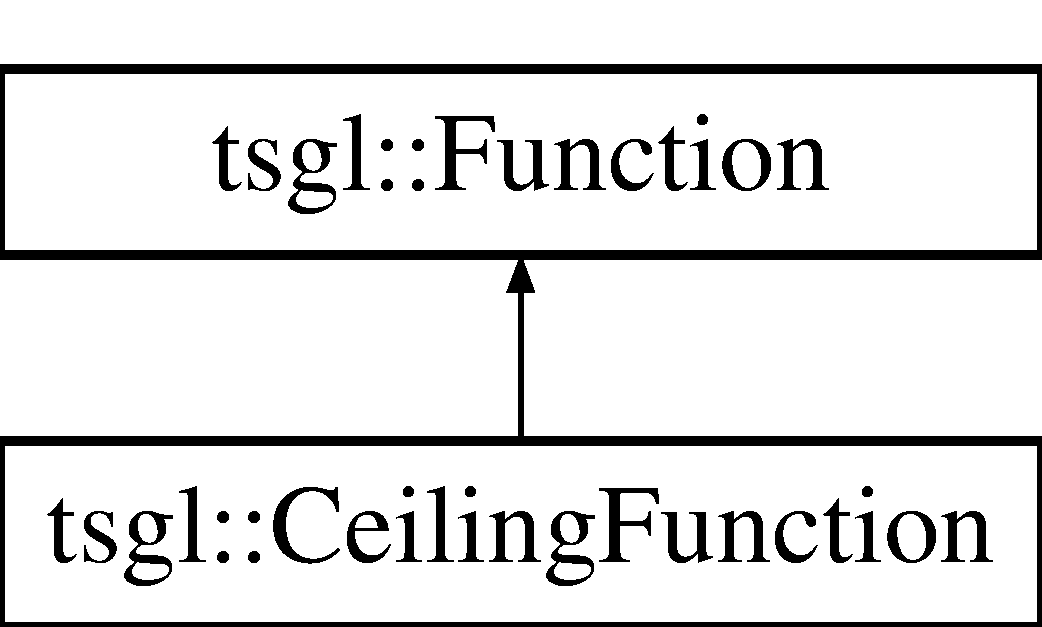
\includegraphics[height=2.000000cm]{classtsgl_1_1_ceiling_function}
\end{center}
\end{figure}
\subsection*{Public Member Functions}
\begin{DoxyCompactItemize}
\item 
virtual Decimal \hyperlink{classtsgl_1_1_ceiling_function_ab47498860b2395e331f203c4025bcb81}{value\-At} (Decimal x) const 
\begin{DoxyCompactList}\small\item\em Method to determine the value of \hyperlink{classtsgl_1_1_ceiling_function}{Ceiling\-Function}. \end{DoxyCompactList}\end{DoxyCompactItemize}


\subsection{Detailed Description}
\hyperlink{classtsgl_1_1_function}{Function} to compute the mathematical ceiling of the input. 

\subsection{Member Function Documentation}
\hypertarget{classtsgl_1_1_ceiling_function_ab47498860b2395e331f203c4025bcb81}{\index{tsgl\-::\-Ceiling\-Function@{tsgl\-::\-Ceiling\-Function}!value\-At@{value\-At}}
\index{value\-At@{value\-At}!tsgl::CeilingFunction@{tsgl\-::\-Ceiling\-Function}}
\subsubsection[{value\-At}]{\setlength{\rightskip}{0pt plus 5cm}virtual Decimal tsgl\-::\-Ceiling\-Function\-::value\-At (
\begin{DoxyParamCaption}
\item[{Decimal}]{x}
\end{DoxyParamCaption}
) const\hspace{0.3cm}{\ttfamily [inline]}, {\ttfamily [virtual]}}}\label{classtsgl_1_1_ceiling_function_ab47498860b2395e331f203c4025bcb81}


Method to determine the value of \hyperlink{classtsgl_1_1_ceiling_function}{Ceiling\-Function}. 

\begin{DoxyReturn}{Returns}
The smallest integer greater than or equal to {\itshape x}. 
\end{DoxyReturn}


Implements \hyperlink{classtsgl_1_1_function_affb7b3b19a04efefa29a9870d666e912}{tsgl\-::\-Function}.



The documentation for this class was generated from the following file\-:\begin{DoxyCompactItemize}
\item 
Function.\-h\end{DoxyCompactItemize}

\hypertarget{structtsgl_1_1_color_float}{}\section{tsgl\+:\+:Color\+Float Struct Reference}
\label{structtsgl_1_1_color_float}\index{tsgl\+::\+Color\+Float@{tsgl\+::\+Color\+Float}}


Floating point R\+G\+B\+A color struct.  




{\ttfamily \#include $<$Color.\+h$>$}

\subsection*{Public Member Functions}
\begin{DoxyCompactItemize}
\item 
\hyperlink{structtsgl_1_1_color_float_a22e82c71a0feedbb7b3e3a7a73b80e30}{Color\+Float} ()
\begin{DoxyCompactList}\small\item\em Default \hyperlink{structtsgl_1_1_color_float}{Color\+Float} constructor method. \end{DoxyCompactList}\item 
\hyperlink{structtsgl_1_1_color_float_a134643b43f1d8acaed32095f04942140}{Color\+Float} (float v, float a=1.\+0f)
\begin{DoxyCompactList}\small\item\em Basic explicit \hyperlink{structtsgl_1_1_color_float}{Color\+Float} constructor method. \end{DoxyCompactList}\item 
\hyperlink{structtsgl_1_1_color_float_a6c46a2073d9e208aa3f07cc04565a489}{Color\+Float} (float r, float g, float b, float a=1.\+0f)
\begin{DoxyCompactList}\small\item\em Full explicit \hyperlink{structtsgl_1_1_color_float}{Color\+Float} constructor method. \end{DoxyCompactList}\item 
std\+::string \hyperlink{structtsgl_1_1_color_float_a1048e8773d65fa1554bc8782e76527ed}{as\+String} ()
\begin{DoxyCompactList}\small\item\em Returns a string representation of the \hyperlink{structtsgl_1_1_color_float}{Color\+Float}. \end{DoxyCompactList}\item 
\hyperlink{structtsgl_1_1_color_float_a4d74b061239eed7eb351422c18e33a37}{operator Color\+H\+S\+V} ()
\begin{DoxyCompactList}\small\item\em Implicit conversion from \hyperlink{structtsgl_1_1_color_float}{Color\+Float} to \hyperlink{structtsgl_1_1_color_h_s_v}{Color\+H\+S\+V}. \end{DoxyCompactList}\item 
\hyperlink{structtsgl_1_1_color_float_a4ef5398fd1ee469dd9b1b43c9ce5c00d}{operator Color\+Int} ()
\begin{DoxyCompactList}\small\item\em Implicit conversion from \hyperlink{structtsgl_1_1_color_float}{Color\+Float} to \hyperlink{structtsgl_1_1_color_int}{Color\+Int}. \end{DoxyCompactList}\item 
\hyperlink{structtsgl_1_1_color_float}{Color\+Float} \hyperlink{structtsgl_1_1_color_float_a09d7cc47ac3d0e23ef7339ccf33111a5}{operator$\ast$} (float f)
\begin{DoxyCompactList}\small\item\em Multiplies the values of a \hyperlink{structtsgl_1_1_color_float}{Color\+Float} by a float. \end{DoxyCompactList}\item 
bool \hyperlink{structtsgl_1_1_color_float_ac29ecf4a36624050af433d691e65651c}{operator==} (\hyperlink{structtsgl_1_1_color_float}{Color\+Float} \&c2)
\begin{DoxyCompactList}\small\item\em Determines if two Color\+Floats are equivalent. \end{DoxyCompactList}\item 
bool \hyperlink{structtsgl_1_1_color_float_afd92fcf8743d931cfbcf405209c923fc}{operator!=} (\hyperlink{structtsgl_1_1_color_float}{Color\+Float} \&c2)
\begin{DoxyCompactList}\small\item\em Determines if two Color\+Floats are {\itshape N\+O\+T} equivalent. \end{DoxyCompactList}\end{DoxyCompactItemize}
\subsection*{Public Attributes}
\begin{DoxyCompactItemize}
\item 
\hypertarget{structtsgl_1_1_color_float_a15c36dbebaccfc982b0b07af95214d10}{}float {\bfseries R}\label{structtsgl_1_1_color_float_a15c36dbebaccfc982b0b07af95214d10}

\item 
\hypertarget{structtsgl_1_1_color_float_a7a7f1659d2f7694625f4a393a57686b4}{}float {\bfseries G}\label{structtsgl_1_1_color_float_a7a7f1659d2f7694625f4a393a57686b4}

\item 
\hypertarget{structtsgl_1_1_color_float_ae0c874ce1bc4a3fb725bbae35411a794}{}float {\bfseries B}\label{structtsgl_1_1_color_float_ae0c874ce1bc4a3fb725bbae35411a794}

\item 
\hypertarget{structtsgl_1_1_color_float_aba05ee650a72ae8e3c4683b54bf192fb}{}float {\bfseries A}\label{structtsgl_1_1_color_float_aba05ee650a72ae8e3c4683b54bf192fb}

\end{DoxyCompactItemize}


\subsection{Detailed Description}
Floating point R\+G\+B\+A color struct. 

\hyperlink{structtsgl_1_1_color_float}{Color\+Float} defines a color with floating point red, green, blue, and alpha components. 
\begin{DoxyParams}{Parameters}
{\em R} & Red component, between 0 and 1 inclusive. \\
\hline
{\em G} & Green component, between 0 and 1 inclusive. \\
\hline
{\em B} & Blue component, between 0 and 1 inclusive. \\
\hline
{\em A} & Alpha component, between 0 and 1 inclusive. \\
\hline
\end{DoxyParams}


\subsection{Constructor \& Destructor Documentation}
\hypertarget{structtsgl_1_1_color_float_a22e82c71a0feedbb7b3e3a7a73b80e30}{}\index{tsgl\+::\+Color\+Float@{tsgl\+::\+Color\+Float}!Color\+Float@{Color\+Float}}
\index{Color\+Float@{Color\+Float}!tsgl\+::\+Color\+Float@{tsgl\+::\+Color\+Float}}
\subsubsection[{Color\+Float}]{\setlength{\rightskip}{0pt plus 5cm}tsgl\+::\+Color\+Float\+::\+Color\+Float (
\begin{DoxyParamCaption}
{}
\end{DoxyParamCaption}
)}\label{structtsgl_1_1_color_float_a22e82c71a0feedbb7b3e3a7a73b80e30}


Default \hyperlink{structtsgl_1_1_color_float}{Color\+Float} constructor method. 

This is the default constructor for the \hyperlink{structtsgl_1_1_color_float}{Color\+Float} struct. \begin{DoxyNote}{Note}
R, G, B, and A are all set to 1.\+0f by default. 
\end{DoxyNote}
\begin{DoxyReturn}{Returns}
A \hyperlink{structtsgl_1_1_color_float}{Color\+Float} struct with default R, G, B, and A values. 
\end{DoxyReturn}


Referenced by operator$\ast$().

\hypertarget{structtsgl_1_1_color_float_a134643b43f1d8acaed32095f04942140}{}\index{tsgl\+::\+Color\+Float@{tsgl\+::\+Color\+Float}!Color\+Float@{Color\+Float}}
\index{Color\+Float@{Color\+Float}!tsgl\+::\+Color\+Float@{tsgl\+::\+Color\+Float}}
\subsubsection[{Color\+Float}]{\setlength{\rightskip}{0pt plus 5cm}tsgl\+::\+Color\+Float\+::\+Color\+Float (
\begin{DoxyParamCaption}
\item[{float}]{v, }
\item[{float}]{a = {\ttfamily 1.0f}}
\end{DoxyParamCaption}
)}\label{structtsgl_1_1_color_float_a134643b43f1d8acaed32095f04942140}


Basic explicit \hyperlink{structtsgl_1_1_color_float}{Color\+Float} constructor method. 

This is the basic explicit constructor for the \hyperlink{structtsgl_1_1_color_float}{Color\+Float} struct. 
\begin{DoxyParams}{Parameters}
{\em v} & The value component of the color. \\
\hline
{\em a} & The alpha component of the struct (set to 1.\+0f by default). \\
\hline
\end{DoxyParams}
\begin{DoxyWarning}{Warning}
An invariant is set where if any of the specified R, G, B, or A values is out of the range 0 -\/ 1 inclusive then an error message is given. 
\end{DoxyWarning}
\begin{DoxyReturn}{Returns}
A \hyperlink{structtsgl_1_1_color_float}{Color\+Float} struct with equal R, G, and B values set to {\ttfamily v}, and the specified A value. 
\end{DoxyReturn}
\hypertarget{structtsgl_1_1_color_float_a6c46a2073d9e208aa3f07cc04565a489}{}\index{tsgl\+::\+Color\+Float@{tsgl\+::\+Color\+Float}!Color\+Float@{Color\+Float}}
\index{Color\+Float@{Color\+Float}!tsgl\+::\+Color\+Float@{tsgl\+::\+Color\+Float}}
\subsubsection[{Color\+Float}]{\setlength{\rightskip}{0pt plus 5cm}tsgl\+::\+Color\+Float\+::\+Color\+Float (
\begin{DoxyParamCaption}
\item[{float}]{r, }
\item[{float}]{g, }
\item[{float}]{b, }
\item[{float}]{a = {\ttfamily 1.0f}}
\end{DoxyParamCaption}
)}\label{structtsgl_1_1_color_float_a6c46a2073d9e208aa3f07cc04565a489}


Full explicit \hyperlink{structtsgl_1_1_color_float}{Color\+Float} constructor method. 

This is the full explicit constructor for the \hyperlink{structtsgl_1_1_color_float}{Color\+Float} struct. 
\begin{DoxyParams}{Parameters}
{\em r} & The red component of the struct. \\
\hline
{\em g} & The green component of the struct. \\
\hline
{\em b} & The blue component of the struct. \\
\hline
{\em a} & The alpha component of the struct (set to 1.\+0f by default). \\
\hline
\end{DoxyParams}
\begin{DoxyWarning}{Warning}
An invariant is set where if any of the specified R, G, B, or A values is out of the range 0 -\/ 1 inclusive then an error message is given. 
\end{DoxyWarning}
\begin{DoxyReturn}{Returns}
A \hyperlink{structtsgl_1_1_color_float}{Color\+Float} struct with the specified R, G, B, and A values. 
\end{DoxyReturn}


\subsection{Member Function Documentation}
\hypertarget{structtsgl_1_1_color_float_a1048e8773d65fa1554bc8782e76527ed}{}\index{tsgl\+::\+Color\+Float@{tsgl\+::\+Color\+Float}!as\+String@{as\+String}}
\index{as\+String@{as\+String}!tsgl\+::\+Color\+Float@{tsgl\+::\+Color\+Float}}
\subsubsection[{as\+String}]{\setlength{\rightskip}{0pt plus 5cm}std\+::string tsgl\+::\+Color\+Float\+::as\+String (
\begin{DoxyParamCaption}
{}
\end{DoxyParamCaption}
)}\label{structtsgl_1_1_color_float_a1048e8773d65fa1554bc8782e76527ed}


Returns a string representation of the \hyperlink{structtsgl_1_1_color_float}{Color\+Float}. 

This function returns a std\+::string representation of the \hyperlink{structtsgl_1_1_color_float}{Color\+Float}. \begin{DoxyReturn}{Returns}
A string representation of the \hyperlink{structtsgl_1_1_color_float}{Color\+Float}. 
\end{DoxyReturn}
\hypertarget{structtsgl_1_1_color_float_a4d74b061239eed7eb351422c18e33a37}{}\index{tsgl\+::\+Color\+Float@{tsgl\+::\+Color\+Float}!operator Color\+H\+S\+V@{operator Color\+H\+S\+V}}
\index{operator Color\+H\+S\+V@{operator Color\+H\+S\+V}!tsgl\+::\+Color\+Float@{tsgl\+::\+Color\+Float}}
\subsubsection[{operator Color\+H\+S\+V}]{\setlength{\rightskip}{0pt plus 5cm}tsgl\+::\+Color\+Float\+::operator {\bf Color\+H\+S\+V} (
\begin{DoxyParamCaption}
{}
\end{DoxyParamCaption}
)}\label{structtsgl_1_1_color_float_a4d74b061239eed7eb351422c18e33a37}


Implicit conversion from \hyperlink{structtsgl_1_1_color_float}{Color\+Float} to \hyperlink{structtsgl_1_1_color_h_s_v}{Color\+H\+S\+V}. 

This defines the implicit conversion operator from a floating point color type (\hyperlink{structtsgl_1_1_color_float}{Color\+Float}) to an H\+S\+V color type (\hyperlink{structtsgl_1_1_color_h_s_v}{Color\+H\+S\+V}). \hypertarget{structtsgl_1_1_color_float_a4ef5398fd1ee469dd9b1b43c9ce5c00d}{}\index{tsgl\+::\+Color\+Float@{tsgl\+::\+Color\+Float}!operator Color\+Int@{operator Color\+Int}}
\index{operator Color\+Int@{operator Color\+Int}!tsgl\+::\+Color\+Float@{tsgl\+::\+Color\+Float}}
\subsubsection[{operator Color\+Int}]{\setlength{\rightskip}{0pt plus 5cm}tsgl\+::\+Color\+Float\+::operator {\bf Color\+Int} (
\begin{DoxyParamCaption}
{}
\end{DoxyParamCaption}
)}\label{structtsgl_1_1_color_float_a4ef5398fd1ee469dd9b1b43c9ce5c00d}


Implicit conversion from \hyperlink{structtsgl_1_1_color_float}{Color\+Float} to \hyperlink{structtsgl_1_1_color_int}{Color\+Int}. 

This defines the implicit conversion operator from a floating point color type (\hyperlink{structtsgl_1_1_color_float}{Color\+Float}) to an integer color type (\hyperlink{structtsgl_1_1_color_int}{Color\+Int}). \hypertarget{structtsgl_1_1_color_float_afd92fcf8743d931cfbcf405209c923fc}{}\index{tsgl\+::\+Color\+Float@{tsgl\+::\+Color\+Float}!operator"!=@{operator"!=}}
\index{operator"!=@{operator"!=}!tsgl\+::\+Color\+Float@{tsgl\+::\+Color\+Float}}
\subsubsection[{operator"!=}]{\setlength{\rightskip}{0pt plus 5cm}bool tsgl\+::\+Color\+Float\+::operator!= (
\begin{DoxyParamCaption}
\item[{{\bf Color\+Float} \&}]{c2}
\end{DoxyParamCaption}
)}\label{structtsgl_1_1_color_float_afd92fcf8743d931cfbcf405209c923fc}


Determines if two Color\+Floats are {\itshape N\+O\+T} equivalent. 

Inequality operator for two Color\+Floats. Determines if they are {\itshape N\+O\+T} equivalent. 
\begin{DoxyParams}{Parameters}
{\em c2} & Reference to the \hyperlink{structtsgl_1_1_color_float}{Color\+Float} struct that is the second one in the inequality comparison. \\
\hline
\end{DoxyParams}
\begin{DoxyNote}{Note}
This function relies on ($\ast$this), which is a dereferenced pointer to the first \hyperlink{structtsgl_1_1_color_float}{Color\+Float} struct in the inequality comparison. (its the one on the left side of the != sign). 
\end{DoxyNote}
\begin{DoxyReturn}{Returns}
true if the two Color\+Floats are not equivalent, false if otherwise. 
\end{DoxyReturn}
\hypertarget{structtsgl_1_1_color_float_a09d7cc47ac3d0e23ef7339ccf33111a5}{}\index{tsgl\+::\+Color\+Float@{tsgl\+::\+Color\+Float}!operator$\ast$@{operator$\ast$}}
\index{operator$\ast$@{operator$\ast$}!tsgl\+::\+Color\+Float@{tsgl\+::\+Color\+Float}}
\subsubsection[{operator$\ast$}]{\setlength{\rightskip}{0pt plus 5cm}{\bf Color\+Float} tsgl\+::\+Color\+Float\+::operator$\ast$ (
\begin{DoxyParamCaption}
\item[{float}]{f}
\end{DoxyParamCaption}
)}\label{structtsgl_1_1_color_float_a09d7cc47ac3d0e23ef7339ccf33111a5}


Multiplies the values of a \hyperlink{structtsgl_1_1_color_float}{Color\+Float} by a float. 

This operator multiplies each of the components of a \hyperlink{structtsgl_1_1_color_float}{Color\+Float} by amount {\ttfamily f}. 
\begin{DoxyParams}{Parameters}
{\em f} & Amount to multiply each component by \\
\hline
\end{DoxyParams}
\begin{DoxyReturn}{Returns}
A new \hyperlink{structtsgl_1_1_color_float}{Color\+Float} constructed as \hyperlink{structtsgl_1_1_color_float}{Color\+Float}(orig.\+R$\ast$f, orig.\+G$\ast$f, orig.\+b$\ast$f, orig.\+A$\ast$f) 
\end{DoxyReturn}
\begin{DoxyNote}{Note}
Individual channels are clamped between 0 and 1. 
\end{DoxyNote}
\hypertarget{structtsgl_1_1_color_float_ac29ecf4a36624050af433d691e65651c}{}\index{tsgl\+::\+Color\+Float@{tsgl\+::\+Color\+Float}!operator==@{operator==}}
\index{operator==@{operator==}!tsgl\+::\+Color\+Float@{tsgl\+::\+Color\+Float}}
\subsubsection[{operator==}]{\setlength{\rightskip}{0pt plus 5cm}bool tsgl\+::\+Color\+Float\+::operator== (
\begin{DoxyParamCaption}
\item[{{\bf Color\+Float} \&}]{c2}
\end{DoxyParamCaption}
)}\label{structtsgl_1_1_color_float_ac29ecf4a36624050af433d691e65651c}


Determines if two Color\+Floats are equivalent. 

Equality operator for two Color\+Floats. Determines if they are equivalent. 
\begin{DoxyParams}{Parameters}
{\em c2} & Reference to the \hyperlink{structtsgl_1_1_color_float}{Color\+Float} struct that is the second one in the equivalence comparison. \\
\hline
\end{DoxyParams}
\begin{DoxyNote}{Note}
This function relies on ($\ast$this), which is a dereferenced pointer to the first \hyperlink{structtsgl_1_1_color_float}{Color\+Float} struct in the comparison. (its the one on the left side of the == sign). 
\end{DoxyNote}
\begin{DoxyReturn}{Returns}
true if the two Color\+Floats are equivalent, false if otherwise. 
\end{DoxyReturn}


The documentation for this struct was generated from the following files\+:\begin{DoxyCompactItemize}
\item 
Color.\+h\item 
Color.\+cpp\end{DoxyCompactItemize}

\hypertarget{structtsgl_1_1_color_h_s_v}{\section{tsgl\-:\-:\-Color\-H\-S\-V \-Struct \-Reference}
\label{structtsgl_1_1_color_h_s_v}\index{tsgl\-::\-Color\-H\-S\-V@{tsgl\-::\-Color\-H\-S\-V}}
}


\-Floating point \-H\-S\-V\-A color struct.  




{\ttfamily \#include $<$\-Color.\-h$>$}

\subsection*{\-Public \-Member \-Functions}
\begin{DoxyCompactItemize}
\item 
\hyperlink{structtsgl_1_1_color_h_s_v_a36b4390ed6aba9f00ac9559ccca74f8a}{\-Color\-H\-S\-V} ()
\begin{DoxyCompactList}\small\item\em \-Constructs a \hyperlink{structtsgl_1_1_color_h_s_v}{\-Color\-H\-S\-V} struct. \end{DoxyCompactList}\item 
\hyperlink{structtsgl_1_1_color_h_s_v_a9ff97b9a0434ab700883b24c3738645d}{\-Color\-H\-S\-V} (float h, float s, float v, float a=1.\-0f)
\begin{DoxyCompactList}\small\item\em \-Explicitly constructs a \hyperlink{structtsgl_1_1_color_h_s_v}{\-Color\-H\-S\-V} struct. \end{DoxyCompactList}\item 
\hyperlink{structtsgl_1_1_color_h_s_v_acac3e7bf684bd8b518ab794ca8bedbf7}{operator Color\-Int} ()
\begin{DoxyCompactList}\small\item\em \-Implicit conversion from \hyperlink{structtsgl_1_1_color_h_s_v}{\-Color\-H\-S\-V} to \hyperlink{structtsgl_1_1_color_int}{\-Color\-Int}. \end{DoxyCompactList}\item 
\hyperlink{structtsgl_1_1_color_h_s_v_a85a62f8d581801540717d3b3cd0ae782}{operator Color\-Float} ()
\begin{DoxyCompactList}\small\item\em \-Implicit conversion from \hyperlink{structtsgl_1_1_color_h_s_v}{\-Color\-H\-S\-V} to \hyperlink{structtsgl_1_1_color_float}{\-Color\-Float}. \end{DoxyCompactList}\item 
std\-::string \hyperlink{structtsgl_1_1_color_h_s_v_ab606504c5b0873b1cef707c523fe5eb1}{as\-String} ()
\begin{DoxyCompactList}\small\item\em \-Returns a string representation of the \hyperlink{structtsgl_1_1_color_h_s_v}{\-Color\-H\-S\-V}. \end{DoxyCompactList}\end{DoxyCompactItemize}
\subsection*{\-Public \-Attributes}
\begin{DoxyCompactItemize}
\item 
\hypertarget{structtsgl_1_1_color_h_s_v_afd87dfc2483324bddf502bf2ba5266b3}{float {\bfseries \-H}}\label{structtsgl_1_1_color_h_s_v_afd87dfc2483324bddf502bf2ba5266b3}

\item 
\hypertarget{structtsgl_1_1_color_h_s_v_a70be2ef38632107a9756740bcca86b45}{float {\bfseries \-S}}\label{structtsgl_1_1_color_h_s_v_a70be2ef38632107a9756740bcca86b45}

\item 
\hypertarget{structtsgl_1_1_color_h_s_v_a56a41d0935fedf853e0ead44c03d0626}{float {\bfseries \-V}}\label{structtsgl_1_1_color_h_s_v_a56a41d0935fedf853e0ead44c03d0626}

\item 
\hypertarget{structtsgl_1_1_color_h_s_v_a188f4a1bb6de8bef57b6913be75e0534}{float {\bfseries \-A}}\label{structtsgl_1_1_color_h_s_v_a188f4a1bb6de8bef57b6913be75e0534}

\end{DoxyCompactItemize}


\subsection{\-Detailed \-Description}
\-Floating point \-H\-S\-V\-A color struct. 

\hyperlink{structtsgl_1_1_color_h_s_v}{\-Color\-H\-S\-V} defines a color with floating point hue, saturation, value, and alpha components. 
\begin{DoxyParams}{\-Parameters}
{\em \-H} & \-Hue component, between 0 and 6 inclusive. \\
\hline
{\em \-S} & \-Saturation component, between 0 and 1 inclusive. \\
\hline
{\em \-V} & \-Value component, between 0 and 1 inclusive. \\
\hline
{\em \-A} & \-Alpha component, between 0 and 1 inclusive. \\
\hline
\end{DoxyParams}


\subsection{\-Constructor \& \-Destructor \-Documentation}
\hypertarget{structtsgl_1_1_color_h_s_v_a36b4390ed6aba9f00ac9559ccca74f8a}{\index{tsgl\-::\-Color\-H\-S\-V@{tsgl\-::\-Color\-H\-S\-V}!\-Color\-H\-S\-V@{\-Color\-H\-S\-V}}
\index{\-Color\-H\-S\-V@{\-Color\-H\-S\-V}!tsgl::ColorHSV@{tsgl\-::\-Color\-H\-S\-V}}
\subsubsection[{\-Color\-H\-S\-V}]{\setlength{\rightskip}{0pt plus 5cm}{\bf tsgl\-::\-Color\-H\-S\-V\-::\-Color\-H\-S\-V} (
\begin{DoxyParamCaption}
{}
\end{DoxyParamCaption}
)}}\label{structtsgl_1_1_color_h_s_v_a36b4390ed6aba9f00ac9559ccca74f8a}


\-Constructs a \hyperlink{structtsgl_1_1_color_h_s_v}{\-Color\-H\-S\-V} struct. 

\-Default constructor for a \hyperlink{structtsgl_1_1_color_h_s_v}{\-Color\-H\-S\-V} struct. \begin{DoxyNote}{\-Note}
\-H is set to 0.\-0f by default. \-S, \-V, and \-A are set to 1.\-0f by default. 
\end{DoxyNote}
\begin{DoxyReturn}{\-Returns}
\-A \hyperlink{structtsgl_1_1_color_h_s_v}{\-Color\-H\-S\-V} struct with default \-H, \-S, \-V, and \-A values. 
\end{DoxyReturn}
\hypertarget{structtsgl_1_1_color_h_s_v_a9ff97b9a0434ab700883b24c3738645d}{\index{tsgl\-::\-Color\-H\-S\-V@{tsgl\-::\-Color\-H\-S\-V}!\-Color\-H\-S\-V@{\-Color\-H\-S\-V}}
\index{\-Color\-H\-S\-V@{\-Color\-H\-S\-V}!tsgl::ColorHSV@{tsgl\-::\-Color\-H\-S\-V}}
\subsubsection[{\-Color\-H\-S\-V}]{\setlength{\rightskip}{0pt plus 5cm}{\bf tsgl\-::\-Color\-H\-S\-V\-::\-Color\-H\-S\-V} (
\begin{DoxyParamCaption}
\item[{float}]{h, }
\item[{float}]{s, }
\item[{float}]{v, }
\item[{float}]{a = {\ttfamily 1.0f}}
\end{DoxyParamCaption}
)}}\label{structtsgl_1_1_color_h_s_v_a9ff97b9a0434ab700883b24c3738645d}


\-Explicitly constructs a \hyperlink{structtsgl_1_1_color_h_s_v}{\-Color\-H\-S\-V} struct. 

\-Explicit constructor for a \hyperlink{structtsgl_1_1_color_h_s_v}{\-Color\-H\-S\-V} struct. 
\begin{DoxyParams}{\-Parameters}
{\em h} & \-Hue component of the \hyperlink{structtsgl_1_1_color_h_s_v}{\-Color\-H\-S\-V} struct. \\
\hline
{\em s} & \-Saturation component of the \hyperlink{structtsgl_1_1_color_h_s_v}{\-Color\-H\-S\-V} struct. \\
\hline
{\em v} & \-Value component of the \hyperlink{structtsgl_1_1_color_h_s_v}{\-Color\-H\-S\-V} struct. \\
\hline
{\em a} & \-Alpha component of the \hyperlink{structtsgl_1_1_color_h_s_v}{\-Color\-H\-S\-V} struct (set to 1.\-0f by default). \\
\hline
\end{DoxyParams}
\begin{DoxyWarning}{\-Warning}
\-An invariant is held for each of the components where if any of them are out of range then an error message is given. 
\end{DoxyWarning}
\begin{DoxyReturn}{\-Returns}
\-A \hyperlink{structtsgl_1_1_color_h_s_v}{\-Color\-H\-S\-V} struct with specified \-H, \-S, \-V, and \-A values. 
\end{DoxyReturn}


\subsection{\-Member \-Function \-Documentation}
\hypertarget{structtsgl_1_1_color_h_s_v_ab606504c5b0873b1cef707c523fe5eb1}{\index{tsgl\-::\-Color\-H\-S\-V@{tsgl\-::\-Color\-H\-S\-V}!as\-String@{as\-String}}
\index{as\-String@{as\-String}!tsgl::ColorHSV@{tsgl\-::\-Color\-H\-S\-V}}
\subsubsection[{as\-String}]{\setlength{\rightskip}{0pt plus 5cm}std\-::string {\bf tsgl\-::\-Color\-H\-S\-V\-::as\-String} (
\begin{DoxyParamCaption}
{}
\end{DoxyParamCaption}
)}}\label{structtsgl_1_1_color_h_s_v_ab606504c5b0873b1cef707c523fe5eb1}


\-Returns a string representation of the \hyperlink{structtsgl_1_1_color_h_s_v}{\-Color\-H\-S\-V}. 

\-This function returns a std\-::string representation of the \hyperlink{structtsgl_1_1_color_h_s_v}{\-Color\-H\-S\-V}. \begin{DoxyReturn}{\-Returns}
\-A string representation of the \hyperlink{structtsgl_1_1_color_h_s_v}{\-Color\-H\-S\-V}. 
\end{DoxyReturn}
\hypertarget{structtsgl_1_1_color_h_s_v_a85a62f8d581801540717d3b3cd0ae782}{\index{tsgl\-::\-Color\-H\-S\-V@{tsgl\-::\-Color\-H\-S\-V}!operator Color\-Float@{operator Color\-Float}}
\index{operator Color\-Float@{operator Color\-Float}!tsgl::ColorHSV@{tsgl\-::\-Color\-H\-S\-V}}
\subsubsection[{operator Color\-Float}]{\setlength{\rightskip}{0pt plus 5cm}tsgl\-::\-Color\-H\-S\-V\-::operator {\bf \-Color\-Float} (
\begin{DoxyParamCaption}
{}
\end{DoxyParamCaption}
)}}\label{structtsgl_1_1_color_h_s_v_a85a62f8d581801540717d3b3cd0ae782}


\-Implicit conversion from \hyperlink{structtsgl_1_1_color_h_s_v}{\-Color\-H\-S\-V} to \hyperlink{structtsgl_1_1_color_float}{\-Color\-Float}. 

\-This defines the implicit conversion operator from an \-H\-S\-V color type (\hyperlink{structtsgl_1_1_color_h_s_v}{\-Color\-H\-S\-V}) to a floating point color type (\hyperlink{structtsgl_1_1_color_float}{\-Color\-Float}). \hypertarget{structtsgl_1_1_color_h_s_v_acac3e7bf684bd8b518ab794ca8bedbf7}{\index{tsgl\-::\-Color\-H\-S\-V@{tsgl\-::\-Color\-H\-S\-V}!operator Color\-Int@{operator Color\-Int}}
\index{operator Color\-Int@{operator Color\-Int}!tsgl::ColorHSV@{tsgl\-::\-Color\-H\-S\-V}}
\subsubsection[{operator Color\-Int}]{\setlength{\rightskip}{0pt plus 5cm}tsgl\-::\-Color\-H\-S\-V\-::operator {\bf \-Color\-Int} (
\begin{DoxyParamCaption}
{}
\end{DoxyParamCaption}
)}}\label{structtsgl_1_1_color_h_s_v_acac3e7bf684bd8b518ab794ca8bedbf7}


\-Implicit conversion from \hyperlink{structtsgl_1_1_color_h_s_v}{\-Color\-H\-S\-V} to \hyperlink{structtsgl_1_1_color_int}{\-Color\-Int}. 

\-This defines the implicit conversion operator from an \-H\-S\-V color type (\hyperlink{structtsgl_1_1_color_h_s_v}{\-Color\-H\-S\-V}) to an integer color type (\hyperlink{structtsgl_1_1_color_int}{\-Color\-Int}). 

\-The documentation for this struct was generated from the following files\-:\begin{DoxyCompactItemize}
\item 
\-Color.\-h\item 
\-Color.\-cpp\end{DoxyCompactItemize}

\hypertarget{structtsgl_1_1_color_int}{}\section{tsgl\+:\+:Color\+Int Struct Reference}
\label{structtsgl_1_1_color_int}\index{tsgl\+::\+Color\+Int@{tsgl\+::\+Color\+Int}}


Integer R\+G\+B\+A color struct.  




{\ttfamily \#include $<$Color.\+h$>$}

\subsection*{Public Member Functions}
\begin{DoxyCompactItemize}
\item 
\hyperlink{structtsgl_1_1_color_int_a7826d99c97b598cadc325716a8b06dbe}{Color\+Int} ()
\begin{DoxyCompactList}\small\item\em Default \hyperlink{structtsgl_1_1_color_int}{Color\+Int} constructor method. \end{DoxyCompactList}\item 
\hyperlink{structtsgl_1_1_color_int_a64b15a8e4e8fb79c13f59da83107a2ea}{Color\+Int} (int v, int a=255)
\begin{DoxyCompactList}\small\item\em Basic explicit \hyperlink{structtsgl_1_1_color_int}{Color\+Int} constructor method. \end{DoxyCompactList}\item 
\hyperlink{structtsgl_1_1_color_int_a0f0dea0c416a290eb4fdaf7583e27285}{Color\+Int} (int r, int g, int b, int a=255)
\begin{DoxyCompactList}\small\item\em Full explicit \hyperlink{structtsgl_1_1_color_int}{Color\+Int} constructor method. \end{DoxyCompactList}\item 
std\+::string \hyperlink{structtsgl_1_1_color_int_af2d134cd71ac7b14eccedca5bde627a0}{as\+String} ()
\begin{DoxyCompactList}\small\item\em Returns a string representation of the \hyperlink{structtsgl_1_1_color_int}{Color\+Int}. \end{DoxyCompactList}\item 
\hyperlink{structtsgl_1_1_color_int_a34855245876c1ccee51625086f671ebf}{operator Color\+Float} ()
\begin{DoxyCompactList}\small\item\em Implicit conversion from \hyperlink{structtsgl_1_1_color_int}{Color\+Int} to \hyperlink{structtsgl_1_1_color_float}{Color\+Float}. \end{DoxyCompactList}\item 
\hyperlink{structtsgl_1_1_color_int_acbd82ad2c6388389aa3474f042a25353}{operator Color\+H\+S\+V} ()
\begin{DoxyCompactList}\small\item\em Implicit conversion from \hyperlink{structtsgl_1_1_color_int}{Color\+Int} to \hyperlink{structtsgl_1_1_color_h_s_v}{Color\+H\+S\+V}. \end{DoxyCompactList}\item 
bool \hyperlink{structtsgl_1_1_color_int_a7d6282c79f42d4ba9a70c4475b8170c2}{operator==} (\hyperlink{structtsgl_1_1_color_int}{Color\+Int} \&c2)
\begin{DoxyCompactList}\small\item\em Determines if two Color\+Ints are equivalent. \end{DoxyCompactList}\item 
bool \hyperlink{structtsgl_1_1_color_int_af83865a1b76eb8c0a5e0fe4bc34fab2d}{operator!=} (\hyperlink{structtsgl_1_1_color_int}{Color\+Int} \&c2)
\begin{DoxyCompactList}\small\item\em Determines if two Color\+Ints are {\itshape N\+O\+T} equivalent. \end{DoxyCompactList}\item 
\hyperlink{structtsgl_1_1_color_int}{Color\+Int} \hyperlink{structtsgl_1_1_color_int_aa6dbbe3d7d1653e16eadc1843a6c3be1}{operator$\ast$} (float f)
\begin{DoxyCompactList}\small\item\em Multiplies the values of a \hyperlink{structtsgl_1_1_color_int}{Color\+Int} by a float. \end{DoxyCompactList}\end{DoxyCompactItemize}
\subsection*{Public Attributes}
\begin{DoxyCompactItemize}
\item 
\hypertarget{structtsgl_1_1_color_int_a72ab1d2040360a98871f96bccdc85da6}{}int {\bfseries R}\label{structtsgl_1_1_color_int_a72ab1d2040360a98871f96bccdc85da6}

\item 
\hypertarget{structtsgl_1_1_color_int_a031a5d8f7e402908648ed67d04341796}{}int {\bfseries G}\label{structtsgl_1_1_color_int_a031a5d8f7e402908648ed67d04341796}

\item 
\hypertarget{structtsgl_1_1_color_int_a3f8bc859cdf8167c3aaaabb493301ea8}{}int {\bfseries B}\label{structtsgl_1_1_color_int_a3f8bc859cdf8167c3aaaabb493301ea8}

\item 
\hypertarget{structtsgl_1_1_color_int_af095bf47ede3084b3d0b4ca5e5638ce3}{}int {\bfseries A}\label{structtsgl_1_1_color_int_af095bf47ede3084b3d0b4ca5e5638ce3}

\end{DoxyCompactItemize}


\subsection{Detailed Description}
Integer R\+G\+B\+A color struct. 

\hyperlink{structtsgl_1_1_color_int}{Color\+Int} defines a color with integer red, green, blue, and alpha components. 
\begin{DoxyParams}{Parameters}
{\em R} & Red component, between 0 and 255 inclusive. \\
\hline
{\em G} & Green component, between 0 and 255 inclusive. \\
\hline
{\em B} & Blue component, between 0 and 255 inclusive. \\
\hline
{\em A} & Alpha component, between 0 and 255 inclusive. \\
\hline
\end{DoxyParams}


\subsection{Constructor \& Destructor Documentation}
\hypertarget{structtsgl_1_1_color_int_a7826d99c97b598cadc325716a8b06dbe}{}\index{tsgl\+::\+Color\+Int@{tsgl\+::\+Color\+Int}!Color\+Int@{Color\+Int}}
\index{Color\+Int@{Color\+Int}!tsgl\+::\+Color\+Int@{tsgl\+::\+Color\+Int}}
\subsubsection[{Color\+Int}]{\setlength{\rightskip}{0pt plus 5cm}tsgl\+::\+Color\+Int\+::\+Color\+Int (
\begin{DoxyParamCaption}
{}
\end{DoxyParamCaption}
)}\label{structtsgl_1_1_color_int_a7826d99c97b598cadc325716a8b06dbe}


Default \hyperlink{structtsgl_1_1_color_int}{Color\+Int} constructor method. 

This is the default constructor for the \hyperlink{structtsgl_1_1_color_int}{Color\+Int} struct. \begin{DoxyNote}{Note}
R, G, B, and A are all set to 255 by default. 
\end{DoxyNote}
\begin{DoxyReturn}{Returns}
A \hyperlink{structtsgl_1_1_color_int}{Color\+Int} struct with default R, G, B, and A values. 
\end{DoxyReturn}


Referenced by operator$\ast$().

\hypertarget{structtsgl_1_1_color_int_a64b15a8e4e8fb79c13f59da83107a2ea}{}\index{tsgl\+::\+Color\+Int@{tsgl\+::\+Color\+Int}!Color\+Int@{Color\+Int}}
\index{Color\+Int@{Color\+Int}!tsgl\+::\+Color\+Int@{tsgl\+::\+Color\+Int}}
\subsubsection[{Color\+Int}]{\setlength{\rightskip}{0pt plus 5cm}tsgl\+::\+Color\+Int\+::\+Color\+Int (
\begin{DoxyParamCaption}
\item[{int}]{v, }
\item[{int}]{a = {\ttfamily 255}}
\end{DoxyParamCaption}
)}\label{structtsgl_1_1_color_int_a64b15a8e4e8fb79c13f59da83107a2ea}


Basic explicit \hyperlink{structtsgl_1_1_color_int}{Color\+Int} constructor method. 

This is the basic explicit constructor for the \hyperlink{structtsgl_1_1_color_int}{Color\+Int} struct. 
\begin{DoxyParams}{Parameters}
{\em v} & The value component of the color. \\
\hline
{\em a} & The alpha component of the struct (set to 255 by default). \\
\hline
\end{DoxyParams}
\begin{DoxyWarning}{Warning}
An invariant is held where if any of the specified values are out of the range 0 -\/ 255 inclusive then an error message is given. 
\end{DoxyWarning}
\begin{DoxyReturn}{Returns}
A \hyperlink{structtsgl_1_1_color_int}{Color\+Int} struct with equal R, G, and B values set to {\ttfamily v}, and the specified A value. 
\end{DoxyReturn}
\hypertarget{structtsgl_1_1_color_int_a0f0dea0c416a290eb4fdaf7583e27285}{}\index{tsgl\+::\+Color\+Int@{tsgl\+::\+Color\+Int}!Color\+Int@{Color\+Int}}
\index{Color\+Int@{Color\+Int}!tsgl\+::\+Color\+Int@{tsgl\+::\+Color\+Int}}
\subsubsection[{Color\+Int}]{\setlength{\rightskip}{0pt plus 5cm}tsgl\+::\+Color\+Int\+::\+Color\+Int (
\begin{DoxyParamCaption}
\item[{int}]{r, }
\item[{int}]{g, }
\item[{int}]{b, }
\item[{int}]{a = {\ttfamily 255}}
\end{DoxyParamCaption}
)}\label{structtsgl_1_1_color_int_a0f0dea0c416a290eb4fdaf7583e27285}


Full explicit \hyperlink{structtsgl_1_1_color_int}{Color\+Int} constructor method. 

This is the full explicit constructor for the \hyperlink{structtsgl_1_1_color_int}{Color\+Int} struct. 
\begin{DoxyParams}{Parameters}
{\em r} & The red component of the \hyperlink{structtsgl_1_1_color_int}{Color\+Int} struct. \\
\hline
{\em g} & The green component of the \hyperlink{structtsgl_1_1_color_int}{Color\+Int} struct. \\
\hline
{\em b} & The blue component of the \hyperlink{structtsgl_1_1_color_int}{Color\+Int} struct. \\
\hline
{\em a} & The alpha component of the \hyperlink{structtsgl_1_1_color_int}{Color\+Int} struct (set to 255 by default). \\
\hline
\end{DoxyParams}
\begin{DoxyWarning}{Warning}
An invariant is held where if any of the specified values are out of the range 0 -\/ 255 inclusive then an error message is given. 
\end{DoxyWarning}
\begin{DoxyReturn}{Returns}
A \hyperlink{structtsgl_1_1_color_int}{Color\+Int} struct with the specified R, G, B, and A values. 
\end{DoxyReturn}


\subsection{Member Function Documentation}
\hypertarget{structtsgl_1_1_color_int_af2d134cd71ac7b14eccedca5bde627a0}{}\index{tsgl\+::\+Color\+Int@{tsgl\+::\+Color\+Int}!as\+String@{as\+String}}
\index{as\+String@{as\+String}!tsgl\+::\+Color\+Int@{tsgl\+::\+Color\+Int}}
\subsubsection[{as\+String}]{\setlength{\rightskip}{0pt plus 5cm}std\+::string tsgl\+::\+Color\+Int\+::as\+String (
\begin{DoxyParamCaption}
{}
\end{DoxyParamCaption}
)}\label{structtsgl_1_1_color_int_af2d134cd71ac7b14eccedca5bde627a0}


Returns a string representation of the \hyperlink{structtsgl_1_1_color_int}{Color\+Int}. 

This function returns a std\+::string representation of the \hyperlink{structtsgl_1_1_color_int}{Color\+Int}. \begin{DoxyReturn}{Returns}
A string representation of the \hyperlink{structtsgl_1_1_color_int}{Color\+Int}. 
\end{DoxyReturn}
\hypertarget{structtsgl_1_1_color_int_a34855245876c1ccee51625086f671ebf}{}\index{tsgl\+::\+Color\+Int@{tsgl\+::\+Color\+Int}!operator Color\+Float@{operator Color\+Float}}
\index{operator Color\+Float@{operator Color\+Float}!tsgl\+::\+Color\+Int@{tsgl\+::\+Color\+Int}}
\subsubsection[{operator Color\+Float}]{\setlength{\rightskip}{0pt plus 5cm}tsgl\+::\+Color\+Int\+::operator {\bf Color\+Float} (
\begin{DoxyParamCaption}
{}
\end{DoxyParamCaption}
)}\label{structtsgl_1_1_color_int_a34855245876c1ccee51625086f671ebf}


Implicit conversion from \hyperlink{structtsgl_1_1_color_int}{Color\+Int} to \hyperlink{structtsgl_1_1_color_float}{Color\+Float}. 

This defines the implicit conversion operator from an integer color type (\hyperlink{structtsgl_1_1_color_int}{Color\+Int}) to a floating point color type (\hyperlink{structtsgl_1_1_color_float}{Color\+Float}). \hypertarget{structtsgl_1_1_color_int_acbd82ad2c6388389aa3474f042a25353}{}\index{tsgl\+::\+Color\+Int@{tsgl\+::\+Color\+Int}!operator Color\+H\+S\+V@{operator Color\+H\+S\+V}}
\index{operator Color\+H\+S\+V@{operator Color\+H\+S\+V}!tsgl\+::\+Color\+Int@{tsgl\+::\+Color\+Int}}
\subsubsection[{operator Color\+H\+S\+V}]{\setlength{\rightskip}{0pt plus 5cm}tsgl\+::\+Color\+Int\+::operator {\bf Color\+H\+S\+V} (
\begin{DoxyParamCaption}
{}
\end{DoxyParamCaption}
)}\label{structtsgl_1_1_color_int_acbd82ad2c6388389aa3474f042a25353}


Implicit conversion from \hyperlink{structtsgl_1_1_color_int}{Color\+Int} to \hyperlink{structtsgl_1_1_color_h_s_v}{Color\+H\+S\+V}. 

This defines the implicit conversion operator from an integer color type (\hyperlink{structtsgl_1_1_color_int}{Color\+Int}) to an H\+S\+V color type (\hyperlink{structtsgl_1_1_color_h_s_v}{Color\+H\+S\+V}). \hypertarget{structtsgl_1_1_color_int_af83865a1b76eb8c0a5e0fe4bc34fab2d}{}\index{tsgl\+::\+Color\+Int@{tsgl\+::\+Color\+Int}!operator"!=@{operator"!=}}
\index{operator"!=@{operator"!=}!tsgl\+::\+Color\+Int@{tsgl\+::\+Color\+Int}}
\subsubsection[{operator"!=}]{\setlength{\rightskip}{0pt plus 5cm}bool tsgl\+::\+Color\+Int\+::operator!= (
\begin{DoxyParamCaption}
\item[{{\bf Color\+Int} \&}]{c2}
\end{DoxyParamCaption}
)}\label{structtsgl_1_1_color_int_af83865a1b76eb8c0a5e0fe4bc34fab2d}


Determines if two Color\+Ints are {\itshape N\+O\+T} equivalent. 

Inequality operator for two Color\+Ints. Determines if they are {\itshape N\+O\+T} equivalent. 
\begin{DoxyParams}{Parameters}
{\em c2} & Reference to the \hyperlink{structtsgl_1_1_color_int}{Color\+Int} struct that is the second one in the inequality comparison. \\
\hline
\end{DoxyParams}
\begin{DoxyNote}{Note}
This function relies on ($\ast$this), which is a dereferenced pointer to the first \hyperlink{structtsgl_1_1_color_int}{Color\+Int} struct in the inequality comparison. (its the one on the left side of the != sign). 
\end{DoxyNote}
\begin{DoxyReturn}{Returns}
true if the two Color\+Ints are not equivalent, false if otherwise. 
\end{DoxyReturn}
\hypertarget{structtsgl_1_1_color_int_aa6dbbe3d7d1653e16eadc1843a6c3be1}{}\index{tsgl\+::\+Color\+Int@{tsgl\+::\+Color\+Int}!operator$\ast$@{operator$\ast$}}
\index{operator$\ast$@{operator$\ast$}!tsgl\+::\+Color\+Int@{tsgl\+::\+Color\+Int}}
\subsubsection[{operator$\ast$}]{\setlength{\rightskip}{0pt plus 5cm}{\bf Color\+Int} tsgl\+::\+Color\+Int\+::operator$\ast$ (
\begin{DoxyParamCaption}
\item[{float}]{f}
\end{DoxyParamCaption}
)}\label{structtsgl_1_1_color_int_aa6dbbe3d7d1653e16eadc1843a6c3be1}


Multiplies the values of a \hyperlink{structtsgl_1_1_color_int}{Color\+Int} by a float. 

This operator multiplies each of the components of a \hyperlink{structtsgl_1_1_color_int}{Color\+Int} by amount {\ttfamily f}. 
\begin{DoxyParams}{Parameters}
{\em f} & Amount to multiply each component by \\
\hline
\end{DoxyParams}
\begin{DoxyReturn}{Returns}
A new \hyperlink{structtsgl_1_1_color_int}{Color\+Int} constructed as \hyperlink{structtsgl_1_1_color_int}{Color\+Int}(orig.\+R$\ast$f, orig.\+G$\ast$f, orig.\+b$\ast$f, orig.\+A$\ast$f) 
\end{DoxyReturn}
\begin{DoxyNote}{Note}
Individual channels are clamped between 0 and M\+A\+X\+\_\+\+C\+O\+L\+O\+R. 
\end{DoxyNote}
\hypertarget{structtsgl_1_1_color_int_a7d6282c79f42d4ba9a70c4475b8170c2}{}\index{tsgl\+::\+Color\+Int@{tsgl\+::\+Color\+Int}!operator==@{operator==}}
\index{operator==@{operator==}!tsgl\+::\+Color\+Int@{tsgl\+::\+Color\+Int}}
\subsubsection[{operator==}]{\setlength{\rightskip}{0pt plus 5cm}bool tsgl\+::\+Color\+Int\+::operator== (
\begin{DoxyParamCaption}
\item[{{\bf Color\+Int} \&}]{c2}
\end{DoxyParamCaption}
)}\label{structtsgl_1_1_color_int_a7d6282c79f42d4ba9a70c4475b8170c2}


Determines if two Color\+Ints are equivalent. 

Equality operator for two Color\+Ints. Determines if they are equivalent. 
\begin{DoxyParams}{Parameters}
{\em c2} & Reference to the \hyperlink{structtsgl_1_1_color_int}{Color\+Int} struct that is the second one in the equivalence comparison. \\
\hline
\end{DoxyParams}
\begin{DoxyNote}{Note}
This function relies on ($\ast$this), which is a dereferenced pointer to the first \hyperlink{structtsgl_1_1_color_int}{Color\+Int} struct in the comparison. (its the one on the left side of the == sign). 
\end{DoxyNote}
\begin{DoxyReturn}{Returns}
true if the two \hyperlink{structtsgl_1_1_color_int}{Color\+Int} are equivalent, false if otherwise. 
\end{DoxyReturn}


The documentation for this struct was generated from the following files\+:\begin{DoxyCompactItemize}
\item 
Color.\+h\item 
Color.\+cpp\end{DoxyCompactItemize}

\hypertarget{classtsgl_1_1_colors}{\section{tsgl\-:\-:Colors Class Reference}
\label{classtsgl_1_1_colors}\index{tsgl\-::\-Colors@{tsgl\-::\-Colors}}
}


Color utility class.  




{\ttfamily \#include $<$Color.\-h$>$}

\subsection*{Static Public Member Functions}
\begin{DoxyCompactItemize}
\item 
static \hyperlink{structtsgl_1_1_color_float}{Color\-Float} \hyperlink{classtsgl_1_1_colors_af610e20b5176294e24fdae4af4f5d6dc}{divide\-Into\-Chromatic\-Sections} (unsigned int total\-Sections, unsigned int index, float value, float alpha=1.\-0f)
\begin{DoxyCompactList}\small\item\em Returns an H\-S\-V\-A color with a hue dependent on the number of sections. \end{DoxyCompactList}\item 
static \hyperlink{structtsgl_1_1_color_float}{Color\-Float} \hyperlink{classtsgl_1_1_colors_ab9c66054f181ca5db5839ede985fb112}{divide\-Into\-Chromatic\-Sections} (unsigned int total\-Sections, unsigned int index)
\begin{DoxyCompactList}\small\item\em Returns an H\-S\-V\-A color with a hue dependent on the number of sections. \end{DoxyCompactList}\item 
static \hyperlink{structtsgl_1_1_color_float}{Color\-Float} \hyperlink{classtsgl_1_1_colors_a0f28a13af4a0fc352a250c23ecc97e4f}{random\-Color} (float alpha=0.\-0f)
\begin{DoxyCompactList}\small\item\em Generates a random color. \end{DoxyCompactList}\item 
static \hyperlink{structtsgl_1_1_color_float}{Color\-Float} \hyperlink{classtsgl_1_1_colors_a26a34b86c0b70fe4984a91a24a0f263f}{blend} (\hyperlink{structtsgl_1_1_color_float}{Color\-Float} c1, \hyperlink{structtsgl_1_1_color_float}{Color\-Float} c2, float bias=0.\-5f)
\begin{DoxyCompactList}\small\item\em Blends two colors with a given bias towards the latter. \end{DoxyCompactList}\item 
static \hyperlink{structtsgl_1_1_color_float}{Color\-Float} \hyperlink{classtsgl_1_1_colors_a93d3fc815542e586dbc1ecf3e984e0b6}{high\-Contrast\-Color} (unsigned int index, int offset=0)
\begin{DoxyCompactList}\small\item\em Returns an H\-S\-V color with high contrast. \end{DoxyCompactList}\end{DoxyCompactItemize}


\subsection{Detailed Description}
Color utility class. 

\hyperlink{classtsgl_1_1_colors}{Colors} defines color utility methods to construct colors. 

\subsection{Member Function Documentation}
\hypertarget{classtsgl_1_1_colors_a26a34b86c0b70fe4984a91a24a0f263f}{\index{tsgl\-::\-Colors@{tsgl\-::\-Colors}!blend@{blend}}
\index{blend@{blend}!tsgl::Colors@{tsgl\-::\-Colors}}
\subsubsection[{blend}]{\setlength{\rightskip}{0pt plus 5cm}{\bf Color\-Float} tsgl\-::\-Colors\-::blend (
\begin{DoxyParamCaption}
\item[{{\bf Color\-Float}}]{c1, }
\item[{{\bf Color\-Float}}]{c2, }
\item[{float}]{bias = {\ttfamily 0.5f}}
\end{DoxyParamCaption}
)\hspace{0.3cm}{\ttfamily [static]}}}\label{classtsgl_1_1_colors_a26a34b86c0b70fe4984a91a24a0f263f}


Blends two colors with a given bias towards the latter. 

This function blends two \hyperlink{structtsgl_1_1_color_float}{Color\-Float} structs together by taking a linear interpolation between the two and returns the result as a new \hyperlink{structtsgl_1_1_color_float}{Color\-Float}. 
\begin{DoxyParams}{Parameters}
{\em c1} & A \hyperlink{structtsgl_1_1_color_float}{Color\-Float}. \\
\hline
{\em c2} & Another \hyperlink{structtsgl_1_1_color_float}{Color\-Float}. \\
\hline
{\em bias} & A bias between 0 and 1 inclusive. A bias of 0 returns c1, a bias of 1 returns c2, and a bias in between returns a linear interpolation. \\
\hline
\end{DoxyParams}
\begin{DoxyWarning}{Warning}
An invariant is held for the bias where if its greater than 1 or less than 0 then an error message is given. 
\end{DoxyWarning}
\begin{DoxyReturn}{Returns}
A \hyperlink{structtsgl_1_1_color_float}{Color\-Float} linearly interpolated between c1 and c2 using the given bias as a weight. 
\end{DoxyReturn}


Referenced by tsgl\-::\-Visual\-Task\-Queue\-::update().

\hypertarget{classtsgl_1_1_colors_af610e20b5176294e24fdae4af4f5d6dc}{\index{tsgl\-::\-Colors@{tsgl\-::\-Colors}!divide\-Into\-Chromatic\-Sections@{divide\-Into\-Chromatic\-Sections}}
\index{divide\-Into\-Chromatic\-Sections@{divide\-Into\-Chromatic\-Sections}!tsgl::Colors@{tsgl\-::\-Colors}}
\subsubsection[{divide\-Into\-Chromatic\-Sections}]{\setlength{\rightskip}{0pt plus 5cm}{\bf Color\-Float} tsgl\-::\-Colors\-::divide\-Into\-Chromatic\-Sections (
\begin{DoxyParamCaption}
\item[{unsigned int}]{total\-Sections, }
\item[{unsigned int}]{index, }
\item[{float}]{value, }
\item[{float}]{alpha = {\ttfamily 1.0f}}
\end{DoxyParamCaption}
)\hspace{0.3cm}{\ttfamily [static]}}}\label{classtsgl_1_1_colors_af610e20b5176294e24fdae4af4f5d6dc}


Returns an H\-S\-V\-A color with a hue dependent on the number of sections. 

This function returns a \hyperlink{structtsgl_1_1_color_float}{Color\-Float} whose hue is calculated from the provided section number and the total number of sections. This function is used for creating a chromatic gradient from one part of the spectrum to another. 
\begin{DoxyParams}{Parameters}
{\em total\-Sections} & Unsigned integer specifying the total number of sections. \\
\hline
{\em index} & Unsigned integer specifying the current section. \\
\hline
{\em value} & Value component, between 0 and 1 inclusive. \\
\hline
{\em alpha} & Alpha component, between 0 and 1 inclusive (set to 1.\-0f by default). \\
\hline
\end{DoxyParams}
\begin{DoxyWarning}{Warning}
An invariant is held where if value or alpha is greater than 1 or less than 0 then an error message is given. 
\end{DoxyWarning}
\begin{DoxyReturn}{Returns}
A \hyperlink{structtsgl_1_1_color_float}{Color\-Float} with a hue calculated as 6.\-0f / sections$\ast$section, saturation of 1.\-0f, and the given value and alpha components. 
\end{DoxyReturn}


Referenced by divide\-Into\-Chromatic\-Sections().

\hypertarget{classtsgl_1_1_colors_ab9c66054f181ca5db5839ede985fb112}{\index{tsgl\-::\-Colors@{tsgl\-::\-Colors}!divide\-Into\-Chromatic\-Sections@{divide\-Into\-Chromatic\-Sections}}
\index{divide\-Into\-Chromatic\-Sections@{divide\-Into\-Chromatic\-Sections}!tsgl::Colors@{tsgl\-::\-Colors}}
\subsubsection[{divide\-Into\-Chromatic\-Sections}]{\setlength{\rightskip}{0pt plus 5cm}{\bf Color\-Float} tsgl\-::\-Colors\-::divide\-Into\-Chromatic\-Sections (
\begin{DoxyParamCaption}
\item[{unsigned int}]{total\-Sections, }
\item[{unsigned int}]{index}
\end{DoxyParamCaption}
)\hspace{0.3cm}{\ttfamily [static]}}}\label{classtsgl_1_1_colors_ab9c66054f181ca5db5839ede985fb112}


Returns an H\-S\-V\-A color with a hue dependent on the number of sections. 

This function returns a \hyperlink{structtsgl_1_1_color_float}{Color\-Float} whose hue is calculated from the provided section number and the total number of sections. This function is used for creating a chromatic gradient from one part of the spectrum to another. 
\begin{DoxyParams}{Parameters}
{\em total\-Sections} & Unsigned integer specifying the total number of sections. \\
\hline
{\em index} & Unsigned integer specifying the current section. \\
\hline
\end{DoxyParams}
\begin{DoxyReturn}{Returns}
A \hyperlink{structtsgl_1_1_color_float}{Color\-Float} with a hue calculated as 6.\-0f / sections$\ast$section, and a saturation, value, and alpha of 1.\-0f. 
\end{DoxyReturn}
\hypertarget{classtsgl_1_1_colors_a93d3fc815542e586dbc1ecf3e984e0b6}{\index{tsgl\-::\-Colors@{tsgl\-::\-Colors}!high\-Contrast\-Color@{high\-Contrast\-Color}}
\index{high\-Contrast\-Color@{high\-Contrast\-Color}!tsgl::Colors@{tsgl\-::\-Colors}}
\subsubsection[{high\-Contrast\-Color}]{\setlength{\rightskip}{0pt plus 5cm}{\bf Color\-Float} tsgl\-::\-Colors\-::high\-Contrast\-Color (
\begin{DoxyParamCaption}
\item[{unsigned int}]{index, }
\item[{int}]{offset = {\ttfamily 0}}
\end{DoxyParamCaption}
)\hspace{0.3cm}{\ttfamily [static]}}}\label{classtsgl_1_1_colors_a93d3fc815542e586dbc1ecf3e984e0b6}


Returns an H\-S\-V color with high contrast. 

This function returns a \hyperlink{structtsgl_1_1_color_h_s_v}{Color\-H\-S\-V} with hue, saturation, and value calculated to contrast highly with colors with nearby indices. 
\begin{DoxyParams}{Parameters}
{\em index} & Unsigned integer representing the current color index. \\
\hline
{\em offset} & Integer offset for the starting position of the calculation. \\
\hline
\end{DoxyParams}
\begin{DoxyReturn}{Returns}
A \hyperlink{structtsgl_1_1_color_h_s_v}{Color\-H\-S\-V} representing a color visually distinct from its neighbors. 
\end{DoxyReturn}


Referenced by tsgl\-::\-Progress\-Bar\-::get\-Rect(), tsgl\-::\-Integral\-Viewer\-::rectangle\-Evaluate(), tsgl\-::\-Visual\-Task\-Queue\-::show\-Legend(), tsgl\-::\-Integral\-Viewer\-::trapezoid\-Evaluate(), and tsgl\-::\-Visual\-Task\-Queue\-::update().

\hypertarget{classtsgl_1_1_colors_a0f28a13af4a0fc352a250c23ecc97e4f}{\index{tsgl\-::\-Colors@{tsgl\-::\-Colors}!random\-Color@{random\-Color}}
\index{random\-Color@{random\-Color}!tsgl::Colors@{tsgl\-::\-Colors}}
\subsubsection[{random\-Color}]{\setlength{\rightskip}{0pt plus 5cm}{\bf Color\-Float} tsgl\-::\-Colors\-::random\-Color (
\begin{DoxyParamCaption}
\item[{float}]{alpha = {\ttfamily 0.0f}}
\end{DoxyParamCaption}
)\hspace{0.3cm}{\ttfamily [static]}}}\label{classtsgl_1_1_colors_a0f28a13af4a0fc352a250c23ecc97e4f}


Generates a random color. 

This function uses rand() to generate a random \hyperlink{structtsgl_1_1_color_float}{Color\-Float} with an optional specified alpha value. 
\begin{DoxyParams}{Parameters}
{\em alpha} & Alpha of the random color to generate. An alpha of 0 will set the alpha to a random legal value (set to 0.\-0f by default). \\
\hline
\end{DoxyParams}
\begin{DoxyWarning}{Warning}
An invariant is held for the alpha value where if its greater than 1 or less than 0 then an error message is given. 
\end{DoxyWarning}
\begin{DoxyReturn}{Returns}
A random \hyperlink{structtsgl_1_1_color_float}{Color\-Float}. 
\end{DoxyReturn}


The documentation for this class was generated from the following files\-:\begin{DoxyCompactItemize}
\item 
Color.\-h\item 
Color.\-cpp\end{DoxyCompactItemize}

\hypertarget{classtsgl_1_1_common_log_function}{}\section{tsgl\+:\+:Common\+Log\+Function Class Reference}
\label{classtsgl_1_1_common_log_function}\index{tsgl\+::\+Common\+Log\+Function@{tsgl\+::\+Common\+Log\+Function}}


\hyperlink{classtsgl_1_1_function}{Function} to compute the base 10 log of the input.  




{\ttfamily \#include $<$Function.\+h$>$}

Inheritance diagram for tsgl\+:\+:Common\+Log\+Function\+:\begin{figure}[H]
\begin{center}
\leavevmode
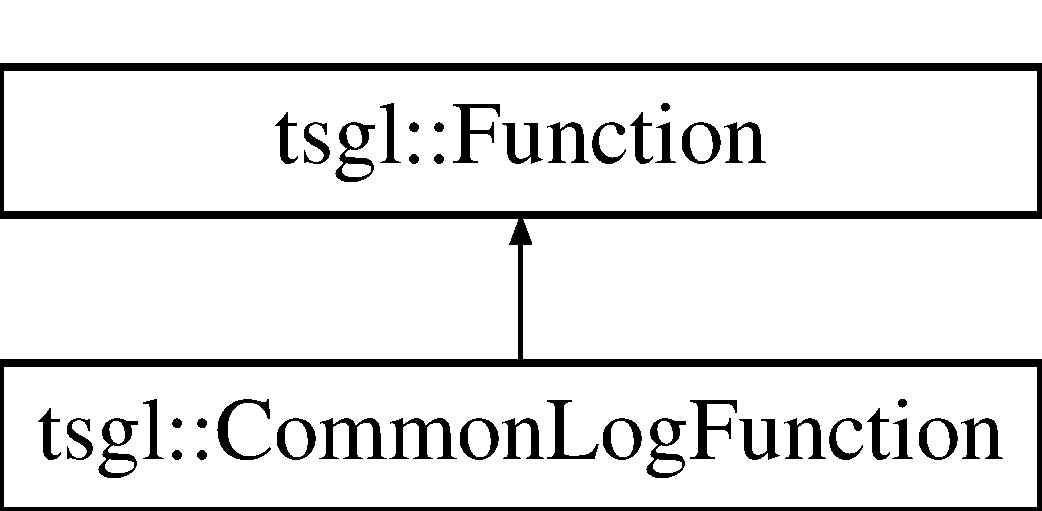
\includegraphics[height=2.000000cm]{classtsgl_1_1_common_log_function}
\end{center}
\end{figure}
\subsection*{Public Member Functions}
\begin{DoxyCompactItemize}
\item 
virtual Decimal \hyperlink{classtsgl_1_1_common_log_function_ac320c0f57c0fc4801bf8eb85f07838d8}{value\+At} (Decimal x) const 
\begin{DoxyCompactList}\small\item\em Method to determine the value of \hyperlink{classtsgl_1_1_common_log_function}{Common\+Log\+Function}. \end{DoxyCompactList}\end{DoxyCompactItemize}


\subsection{Detailed Description}
\hyperlink{classtsgl_1_1_function}{Function} to compute the base 10 log of the input. 

\subsection{Member Function Documentation}
\hypertarget{classtsgl_1_1_common_log_function_ac320c0f57c0fc4801bf8eb85f07838d8}{}\index{tsgl\+::\+Common\+Log\+Function@{tsgl\+::\+Common\+Log\+Function}!value\+At@{value\+At}}
\index{value\+At@{value\+At}!tsgl\+::\+Common\+Log\+Function@{tsgl\+::\+Common\+Log\+Function}}
\subsubsection[{value\+At}]{\setlength{\rightskip}{0pt plus 5cm}virtual Decimal tsgl\+::\+Common\+Log\+Function\+::value\+At (
\begin{DoxyParamCaption}
\item[{Decimal}]{x}
\end{DoxyParamCaption}
) const\hspace{0.3cm}{\ttfamily [inline]}, {\ttfamily [virtual]}}\label{classtsgl_1_1_common_log_function_ac320c0f57c0fc4801bf8eb85f07838d8}


Method to determine the value of \hyperlink{classtsgl_1_1_common_log_function}{Common\+Log\+Function}. 

\begin{DoxyReturn}{Returns}
The base 10 log of {\itshape x}. 
\end{DoxyReturn}


Implements \hyperlink{classtsgl_1_1_function_affb7b3b19a04efefa29a9870d666e912}{tsgl\+::\+Function}.



The documentation for this class was generated from the following file\+:\begin{DoxyCompactItemize}
\item 
Function.\+h\end{DoxyCompactItemize}

\hypertarget{classtsgl_1_1_concave_polygon}{\section{tsgl\-:\-:Concave\-Polygon Class Reference}
\label{classtsgl_1_1_concave_polygon}\index{tsgl\-::\-Concave\-Polygon@{tsgl\-::\-Concave\-Polygon}}
}


Draw an arbitrary Concave polygon with colored vertices.  




{\ttfamily \#include $<$Concave\-Polygon.\-h$>$}

Inheritance diagram for tsgl\-:\-:Concave\-Polygon\-:\begin{figure}[H]
\begin{center}
\leavevmode
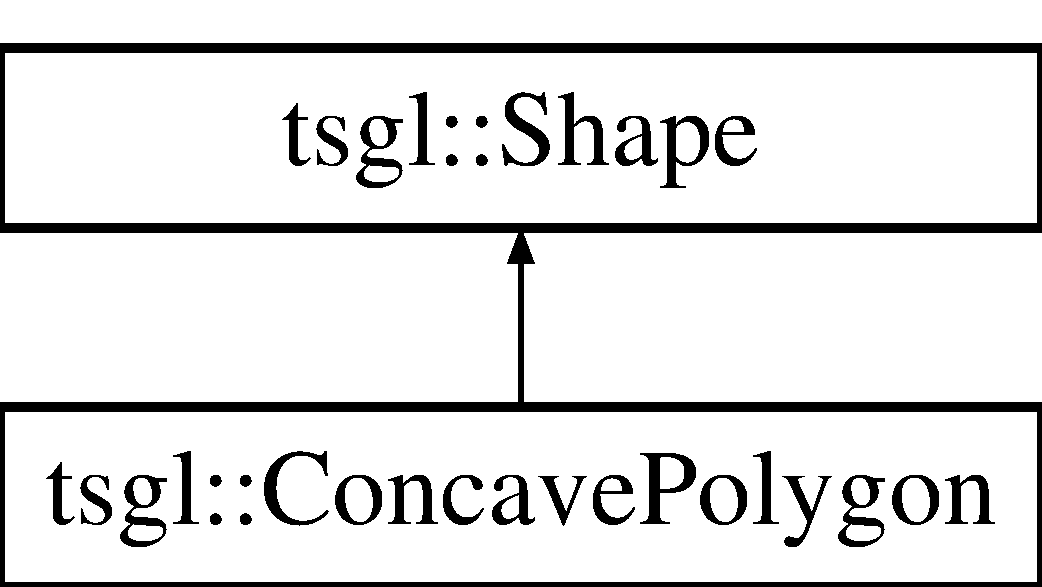
\includegraphics[height=2.000000cm]{classtsgl_1_1_concave_polygon}
\end{center}
\end{figure}
\subsection*{Public Member Functions}
\begin{DoxyCompactItemize}
\item 
\hyperlink{classtsgl_1_1_concave_polygon_a1bb43589a1a992f14111e6a7157f0d7a}{Concave\-Polygon} (int num\-Vertices)
\begin{DoxyCompactList}\small\item\em Explicitly constructs a new \hyperlink{classtsgl_1_1_concave_polygon}{Concave\-Polygon}. \end{DoxyCompactList}\item 
\hyperlink{classtsgl_1_1_concave_polygon_ae1465a7135bb7ef4aa00584fa63b2530}{$\sim$\-Concave\-Polygon} ()
\begin{DoxyCompactList}\small\item\em Destroys a \hyperlink{classtsgl_1_1_concave_polygon}{Concave\-Polygon} object. \end{DoxyCompactList}\item 
bool \hyperlink{classtsgl_1_1_concave_polygon_a0fdc4936df5e1bff64031041fa84fee5}{intersects} (float p0\-\_\-x, float p0\-\_\-y, float p1\-\_\-x, float p1\-\_\-y, float p2\-\_\-x, float p2\-\_\-y, float p3\-\_\-x, float p3\-\_\-y)
\begin{DoxyCompactList}\small\item\em Determines if two lines intersect. \end{DoxyCompactList}\item 
bool \hyperlink{classtsgl_1_1_concave_polygon_afb5de38c8571d6cc808aeaec000f4522}{point\-In\-Triangle} (float px, float py, float x1, float y1, float x2, float y2, float x3, float y3)
\begin{DoxyCompactList}\small\item\em Determines whether a point resides inside of a \hyperlink{classtsgl_1_1_triangle}{Triangle}. \end{DoxyCompactList}\item 
void \hyperlink{classtsgl_1_1_concave_polygon_ae2675ff0bf54cc7092a9ab3418dcab30}{add\-Vertex} (int x, int y, const \hyperlink{structtsgl_1_1_color_float}{Color\-Float} \&color)
\begin{DoxyCompactList}\small\item\em Adds another vertex to a \hyperlink{classtsgl_1_1_concave_polygon}{Concave\-Polygon}. \end{DoxyCompactList}\item 
void \hyperlink{classtsgl_1_1_concave_polygon_a06d759932483ae2b54bb807db20cbc4a}{draw} ()
\begin{DoxyCompactList}\small\item\em Draw the \hyperlink{classtsgl_1_1_concave_polygon}{Concave\-Polygon}. \end{DoxyCompactList}\end{DoxyCompactItemize}
\subsection*{Static Public Member Functions}
\begin{DoxyCompactItemize}
\item 
static void \hyperlink{classtsgl_1_1_concave_polygon_ace68fa148735bf43d9648cb58a04ac46}{run\-Tests} ()
\begin{DoxyCompactList}\small\item\em Runs the Unit tests. \end{DoxyCompactList}\end{DoxyCompactItemize}
\subsection*{Additional Inherited Members}


\subsection{Detailed Description}
Draw an arbitrary Concave polygon with colored vertices. 

\hyperlink{classtsgl_1_1_concave_polygon}{Concave\-Polygon} is a class for holding vertex data for a triangle strip with colored vertices.

Vertices are drawn in triangle strip format, where the first three vertices make up the first triangle, the next vertex plus the previous two make up the second triangle, and so on.

This method is optimized for long lists and offers a marked improvement over drawing individual \hyperlink{classtsgl_1_1_triangle}{Triangle} instances. \begin{DoxyNote}{Note}
The \hyperlink{classtsgl_1_1_concave_polygon_ae2675ff0bf54cc7092a9ab3418dcab30}{add\-Vertex()} method must be called the same number of times as specified in the constructor. 

Calling \hyperlink{classtsgl_1_1_concave_polygon_ae2675ff0bf54cc7092a9ab3418dcab30}{add\-Vertex()} after all vertices have been added will do nothing. 

Calling \hyperlink{classtsgl_1_1_concave_polygon_a06d759932483ae2b54bb807db20cbc4a}{draw()} before all vertices have been added will do nothing. 
\end{DoxyNote}


\subsection{Constructor \& Destructor Documentation}
\hypertarget{classtsgl_1_1_concave_polygon_a1bb43589a1a992f14111e6a7157f0d7a}{\index{tsgl\-::\-Concave\-Polygon@{tsgl\-::\-Concave\-Polygon}!Concave\-Polygon@{Concave\-Polygon}}
\index{Concave\-Polygon@{Concave\-Polygon}!tsgl::ConcavePolygon@{tsgl\-::\-Concave\-Polygon}}
\subsubsection[{Concave\-Polygon}]{\setlength{\rightskip}{0pt plus 5cm}tsgl\-::\-Concave\-Polygon\-::\-Concave\-Polygon (
\begin{DoxyParamCaption}
\item[{int}]{num\-Vertices}
\end{DoxyParamCaption}
)}}\label{classtsgl_1_1_concave_polygon_a1bb43589a1a992f14111e6a7157f0d7a}


Explicitly constructs a new \hyperlink{classtsgl_1_1_concave_polygon}{Concave\-Polygon}. 

Explicit constructor for a \hyperlink{classtsgl_1_1_concave_polygon}{Concave\-Polygon} object. 
\begin{DoxyParams}{Parameters}
{\em num\-Vertices} & The number of vertices the complete \hyperlink{classtsgl_1_1_concave_polygon}{Concave\-Polygon} will have. \\
\hline
\end{DoxyParams}
\begin{DoxyWarning}{Warning}
An invariant is held where if v is less than 3 then an error message is given. 
\end{DoxyWarning}
\begin{DoxyReturn}{Returns}
A new \hyperlink{classtsgl_1_1_concave_polygon}{Concave\-Polygon} with a buffer for storing the specified number of vertices. 
\end{DoxyReturn}
\hypertarget{classtsgl_1_1_concave_polygon_ae1465a7135bb7ef4aa00584fa63b2530}{\index{tsgl\-::\-Concave\-Polygon@{tsgl\-::\-Concave\-Polygon}!$\sim$\-Concave\-Polygon@{$\sim$\-Concave\-Polygon}}
\index{$\sim$\-Concave\-Polygon@{$\sim$\-Concave\-Polygon}!tsgl::ConcavePolygon@{tsgl\-::\-Concave\-Polygon}}
\subsubsection[{$\sim$\-Concave\-Polygon}]{\setlength{\rightskip}{0pt plus 5cm}tsgl\-::\-Concave\-Polygon\-::$\sim$\-Concave\-Polygon (
\begin{DoxyParamCaption}
{}
\end{DoxyParamCaption}
)}}\label{classtsgl_1_1_concave_polygon_ae1465a7135bb7ef4aa00584fa63b2530}


Destroys a \hyperlink{classtsgl_1_1_concave_polygon}{Concave\-Polygon} object. 

Destructor for a \hyperlink{classtsgl_1_1_concave_polygon}{Concave\-Polygon} object.

Frees up memory that was allocated to a \hyperlink{classtsgl_1_1_concave_polygon}{Concave\-Polygon} object. 

\subsection{Member Function Documentation}
\hypertarget{classtsgl_1_1_concave_polygon_ae2675ff0bf54cc7092a9ab3418dcab30}{\index{tsgl\-::\-Concave\-Polygon@{tsgl\-::\-Concave\-Polygon}!add\-Vertex@{add\-Vertex}}
\index{add\-Vertex@{add\-Vertex}!tsgl::ConcavePolygon@{tsgl\-::\-Concave\-Polygon}}
\subsubsection[{add\-Vertex}]{\setlength{\rightskip}{0pt plus 5cm}void tsgl\-::\-Concave\-Polygon\-::add\-Vertex (
\begin{DoxyParamCaption}
\item[{int}]{x, }
\item[{int}]{y, }
\item[{const {\bf Color\-Float} \&}]{color}
\end{DoxyParamCaption}
)}}\label{classtsgl_1_1_concave_polygon_ae2675ff0bf54cc7092a9ab3418dcab30}


Adds another vertex to a \hyperlink{classtsgl_1_1_concave_polygon}{Concave\-Polygon}. 

This function initializes the next vertex in the \hyperlink{classtsgl_1_1_polyline}{Polyline} and adds it to a \hyperlink{classtsgl_1_1_concave_polygon}{Concave\-Polygon} buffer. 
\begin{DoxyParams}{Parameters}
{\em x} & The x position of the vertex. \\
\hline
{\em y} & The y position of the vertex. \\
\hline
{\em color} & The reference variable of the color of the vertex. \\
\hline
\end{DoxyParams}
\begin{DoxyNote}{Note}
This function does nothing if the vertex buffer is already full. 

A message is given indicating that the vertex buffer is full. 
\end{DoxyNote}


Referenced by tsgl\-::\-Canvas\-::draw\-Concave\-Polygon().

\hypertarget{classtsgl_1_1_concave_polygon_a06d759932483ae2b54bb807db20cbc4a}{\index{tsgl\-::\-Concave\-Polygon@{tsgl\-::\-Concave\-Polygon}!draw@{draw}}
\index{draw@{draw}!tsgl::ConcavePolygon@{tsgl\-::\-Concave\-Polygon}}
\subsubsection[{draw}]{\setlength{\rightskip}{0pt plus 5cm}void tsgl\-::\-Concave\-Polygon\-::draw (
\begin{DoxyParamCaption}
{}
\end{DoxyParamCaption}
)\hspace{0.3cm}{\ttfamily [virtual]}}}\label{classtsgl_1_1_concave_polygon_a06d759932483ae2b54bb807db20cbc4a}


Draw the \hyperlink{classtsgl_1_1_concave_polygon}{Concave\-Polygon}. 

This function actually draws the \hyperlink{classtsgl_1_1_concave_polygon}{Concave\-Polygon} to the \hyperlink{classtsgl_1_1_canvas}{Canvas}. \begin{DoxyNote}{Note}
This function does nothing if the vertex buffer is not yet full. 

A message is given indicating that the \hyperlink{classtsgl_1_1_concave_polygon}{Concave\-Polygon} is {\itshape N\-O\-T} ready to be drawn yet (vertex buffer = not full). 
\end{DoxyNote}
\begin{DoxyWarning}{Warning}
This is an order of n-\/cubed operation, and is thus {\bfseries V\-E\-R\-Y S\-L\-O\-W}. 
\end{DoxyWarning}


Implements \hyperlink{classtsgl_1_1_shape_af78b1627b97d621824ce86db214e2402}{tsgl\-::\-Shape}.

\hypertarget{classtsgl_1_1_concave_polygon_a0fdc4936df5e1bff64031041fa84fee5}{\index{tsgl\-::\-Concave\-Polygon@{tsgl\-::\-Concave\-Polygon}!intersects@{intersects}}
\index{intersects@{intersects}!tsgl::ConcavePolygon@{tsgl\-::\-Concave\-Polygon}}
\subsubsection[{intersects}]{\setlength{\rightskip}{0pt plus 5cm}bool tsgl\-::\-Concave\-Polygon\-::intersects (
\begin{DoxyParamCaption}
\item[{float}]{p0\-\_\-x, }
\item[{float}]{p0\-\_\-y, }
\item[{float}]{p1\-\_\-x, }
\item[{float}]{p1\-\_\-y, }
\item[{float}]{p2\-\_\-x, }
\item[{float}]{p2\-\_\-y, }
\item[{float}]{p3\-\_\-x, }
\item[{float}]{p3\-\_\-y}
\end{DoxyParamCaption}
)}}\label{classtsgl_1_1_concave_polygon_a0fdc4936df5e1bff64031041fa84fee5}


Determines if two lines intersect. 

Simulates two lines inside of a \hyperlink{classtsgl_1_1_concave_polygon}{Concave\-Polygon} object and determines whether those two lines intersect. 
\begin{DoxyParams}{Parameters}
{\em p0\-\_\-x} & The x coordinate of the first point of the first line. \\
\hline
{\em p0\-\_\-y} & The y coordinate of the first point of the first line. \\
\hline
{\em p1\-\_\-x} & The x coordinate of the second point of the first line. \\
\hline
{\em p1\-\_\-y} & The y coordinate of the second point of the first line. \\
\hline
{\em p2\-\_\-x} & The x coordinate of the first point of the second line. \\
\hline
{\em p2\-\_\-y} & The y coordinate of the first point of the second line. \\
\hline
{\em p3\-\_\-x} & The x coordinate of the second point of the second line. \\
\hline
{\em p3\-\_\-y} & The y coordinate of the second point of the second line. \\
\hline
\end{DoxyParams}
\begin{DoxyReturn}{Returns}
true if the lines do intersect, false if otherwise. 
\end{DoxyReturn}


Referenced by draw().

\hypertarget{classtsgl_1_1_concave_polygon_afb5de38c8571d6cc808aeaec000f4522}{\index{tsgl\-::\-Concave\-Polygon@{tsgl\-::\-Concave\-Polygon}!point\-In\-Triangle@{point\-In\-Triangle}}
\index{point\-In\-Triangle@{point\-In\-Triangle}!tsgl::ConcavePolygon@{tsgl\-::\-Concave\-Polygon}}
\subsubsection[{point\-In\-Triangle}]{\setlength{\rightskip}{0pt plus 5cm}bool tsgl\-::\-Concave\-Polygon\-::point\-In\-Triangle (
\begin{DoxyParamCaption}
\item[{float}]{px, }
\item[{float}]{py, }
\item[{float}]{x1, }
\item[{float}]{y1, }
\item[{float}]{x2, }
\item[{float}]{y2, }
\item[{float}]{x3, }
\item[{float}]{y3}
\end{DoxyParamCaption}
)}}\label{classtsgl_1_1_concave_polygon_afb5de38c8571d6cc808aeaec000f4522}


Determines whether a point resides inside of a \hyperlink{classtsgl_1_1_triangle}{Triangle}. 

Simulates a \hyperlink{classtsgl_1_1_triangle}{Triangle} and point inside of a \hyperlink{classtsgl_1_1_concave_polygon}{Concave\-Polygon} object and determines whether the point resides inside of the \hyperlink{classtsgl_1_1_triangle}{Triangle}. 
\begin{DoxyParams}{Parameters}
{\em px} & The x coordinate of the point. \\
\hline
{\em py} & The y coordinate of the point. \\
\hline
{\em x1} & The x coordinate of the first vertex of the \hyperlink{classtsgl_1_1_triangle}{Triangle}. \\
\hline
{\em y1} & The y coordinate of the first vertex of the \hyperlink{classtsgl_1_1_triangle}{Triangle}. \\
\hline
{\em x2} & The x coordinate of the second vertex of the \hyperlink{classtsgl_1_1_triangle}{Triangle}. \\
\hline
{\em y2} & The y coordinate of the second vertex of the \hyperlink{classtsgl_1_1_triangle}{Triangle}. \\
\hline
{\em x3} & The x coordinate of the third vertex of the \hyperlink{classtsgl_1_1_triangle}{Triangle}. \\
\hline
{\em y3} & The y coordinate of the third vertex of the \hyperlink{classtsgl_1_1_triangle}{Triangle}. \\
\hline
\end{DoxyParams}
\begin{DoxyReturn}{Returns}
true if the point does reside in the \hyperlink{classtsgl_1_1_triangle}{Triangle}, false if otherwise. 
\end{DoxyReturn}


Referenced by draw().

\hypertarget{classtsgl_1_1_concave_polygon_ace68fa148735bf43d9648cb58a04ac46}{\index{tsgl\-::\-Concave\-Polygon@{tsgl\-::\-Concave\-Polygon}!run\-Tests@{run\-Tests}}
\index{run\-Tests@{run\-Tests}!tsgl::ConcavePolygon@{tsgl\-::\-Concave\-Polygon}}
\subsubsection[{run\-Tests}]{\setlength{\rightskip}{0pt plus 5cm}void tsgl\-::\-Concave\-Polygon\-::run\-Tests (
\begin{DoxyParamCaption}
{}
\end{DoxyParamCaption}
)\hspace{0.3cm}{\ttfamily [static]}}}\label{classtsgl_1_1_concave_polygon_ace68fa148735bf43d9648cb58a04ac46}


Runs the Unit tests. 

Runs the Unit tests for the \hyperlink{classtsgl_1_1_concave_polygon}{Concave\-Polygon} class. \hyperlink{classtsgl_1_1_concave_polygon_a0fdc4936df5e1bff64031041fa84fee5}{intersects()} and \hyperlink{classtsgl_1_1_concave_polygon_afb5de38c8571d6cc808aeaec000f4522}{point\-In\-Triangle()} are tested. 

The documentation for this class was generated from the following files\-:\begin{DoxyCompactItemize}
\item 
Concave\-Polygon.\-h\item 
Concave\-Polygon.\-cpp\end{DoxyCompactItemize}

\hypertarget{classtsgl_1_1_convex_polygon}{}\section{tsgl\+:\+:Convex\+Polygon Class Reference}
\label{classtsgl_1_1_convex_polygon}\index{tsgl\+::\+Convex\+Polygon@{tsgl\+::\+Convex\+Polygon}}


Draw an arbitrary Convex polygon with colored vertices.  




{\ttfamily \#include $<$Convex\+Polygon.\+h$>$}

Inheritance diagram for tsgl\+:\+:Convex\+Polygon\+:\begin{figure}[H]
\begin{center}
\leavevmode
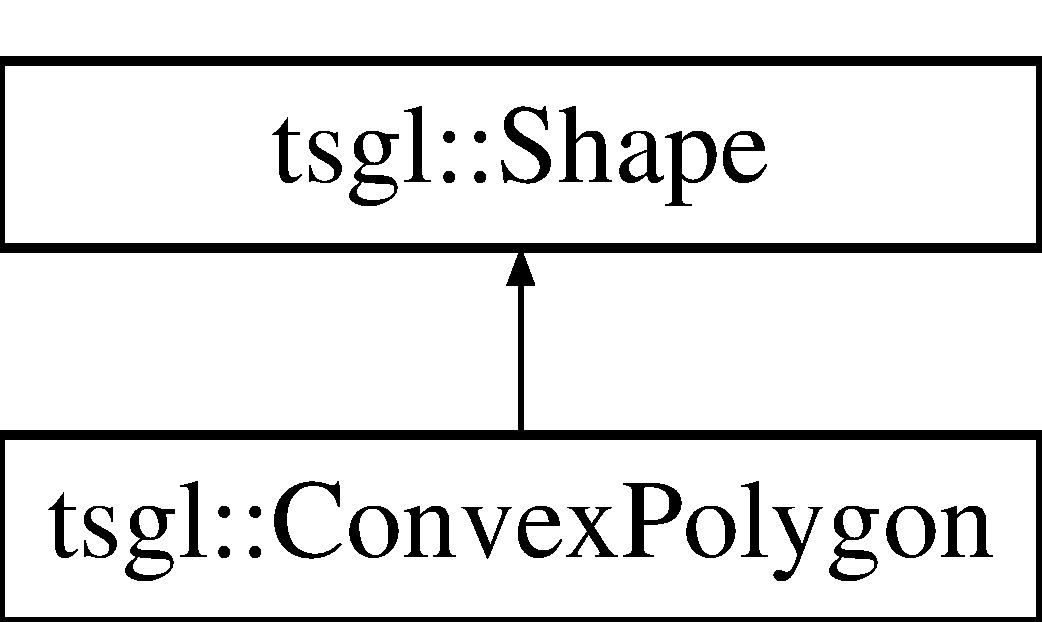
\includegraphics[height=2.000000cm]{classtsgl_1_1_convex_polygon}
\end{center}
\end{figure}
\subsection*{Public Member Functions}
\begin{DoxyCompactItemize}
\item 
\hyperlink{classtsgl_1_1_convex_polygon_ae9d826f3b3155fe84016e6efbcbd2b64}{Convex\+Polygon} (int num\+Vertices)
\begin{DoxyCompactList}\small\item\em Explicitly constructs a new \hyperlink{classtsgl_1_1_convex_polygon}{Convex\+Polygon}. \end{DoxyCompactList}\item 
\hyperlink{classtsgl_1_1_convex_polygon_a46a5bde76d6843d47c754a04cc847e64}{$\sim$\+Convex\+Polygon} ()
\begin{DoxyCompactList}\small\item\em Destroys a \hyperlink{classtsgl_1_1_convex_polygon}{Convex\+Polygon} object. \end{DoxyCompactList}\item 
void \hyperlink{classtsgl_1_1_convex_polygon_a60d17a5ac80a796d05dfeff855791cc0}{add\+Vertex} (int x, int y, const \hyperlink{structtsgl_1_1_color_float}{Color\+Float} \&color)
\begin{DoxyCompactList}\small\item\em Adds another vertex to a \hyperlink{classtsgl_1_1_convex_polygon}{Convex\+Polygon}. \end{DoxyCompactList}\item 
void \hyperlink{classtsgl_1_1_convex_polygon_add4d4971a5d22385eebbfe771af916b5}{draw} ()
\begin{DoxyCompactList}\small\item\em Draw the \hyperlink{classtsgl_1_1_convex_polygon}{Convex\+Polygon}. \end{DoxyCompactList}\end{DoxyCompactItemize}
\subsection*{Static Public Member Functions}
\begin{DoxyCompactItemize}
\item 
static void \hyperlink{classtsgl_1_1_convex_polygon_ac309bc2b2f142b0a02b9dc38e901daeb}{run\+Tests} ()
\begin{DoxyCompactList}\small\item\em Runs the Unit tests. \end{DoxyCompactList}\end{DoxyCompactItemize}
\subsection*{Additional Inherited Members}


\subsection{Detailed Description}
Draw an arbitrary Convex polygon with colored vertices. 

\hyperlink{classtsgl_1_1_convex_polygon}{Convex\+Polygon} is a class for holding vertex data for a triangle strip with colored vertices.

Vertices are drawn in triangle strip format, where the first three vertices make up the first triangle, the next vertex plus the previous two make up the second triangle, and so on.

This method is optimized for long lists and offers a marked improvement over drawing individual \hyperlink{classtsgl_1_1_triangle}{Triangle} instances. \begin{DoxyNote}{Note}
The \hyperlink{classtsgl_1_1_convex_polygon_a60d17a5ac80a796d05dfeff855791cc0}{add\+Vertex()} method must be called the same number of times as specified in the constructor. 

Calling \hyperlink{classtsgl_1_1_convex_polygon_a60d17a5ac80a796d05dfeff855791cc0}{add\+Vertex()} after all vertices have been added will do nothing. 

Calling \hyperlink{classtsgl_1_1_convex_polygon_add4d4971a5d22385eebbfe771af916b5}{draw()} before all vertices have been added will do nothing. 
\end{DoxyNote}


\subsection{Constructor \& Destructor Documentation}
\hypertarget{classtsgl_1_1_convex_polygon_ae9d826f3b3155fe84016e6efbcbd2b64}{}\index{tsgl\+::\+Convex\+Polygon@{tsgl\+::\+Convex\+Polygon}!Convex\+Polygon@{Convex\+Polygon}}
\index{Convex\+Polygon@{Convex\+Polygon}!tsgl\+::\+Convex\+Polygon@{tsgl\+::\+Convex\+Polygon}}
\subsubsection[{Convex\+Polygon}]{\setlength{\rightskip}{0pt plus 5cm}tsgl\+::\+Convex\+Polygon\+::\+Convex\+Polygon (
\begin{DoxyParamCaption}
\item[{int}]{num\+Vertices}
\end{DoxyParamCaption}
)}\label{classtsgl_1_1_convex_polygon_ae9d826f3b3155fe84016e6efbcbd2b64}


Explicitly constructs a new \hyperlink{classtsgl_1_1_convex_polygon}{Convex\+Polygon}. 

Explicit constructor for a Convex Polygon object. 
\begin{DoxyParams}{Parameters}
{\em num\+Vertices} & the number of vertices the complete \hyperlink{classtsgl_1_1_convex_polygon}{Convex\+Polygon} will have. \\
\hline
\end{DoxyParams}
\begin{DoxyWarning}{Warning}
An invariant is held where if v is less than 3 then an error message is given. 
\end{DoxyWarning}
\begin{DoxyReturn}{Returns}
A new \hyperlink{classtsgl_1_1_convex_polygon}{Convex\+Polygon} with a buffer for storing the specified numbered of vertices. 
\end{DoxyReturn}
\hypertarget{classtsgl_1_1_convex_polygon_a46a5bde76d6843d47c754a04cc847e64}{}\index{tsgl\+::\+Convex\+Polygon@{tsgl\+::\+Convex\+Polygon}!````~Convex\+Polygon@{$\sim$\+Convex\+Polygon}}
\index{````~Convex\+Polygon@{$\sim$\+Convex\+Polygon}!tsgl\+::\+Convex\+Polygon@{tsgl\+::\+Convex\+Polygon}}
\subsubsection[{$\sim$\+Convex\+Polygon}]{\setlength{\rightskip}{0pt plus 5cm}tsgl\+::\+Convex\+Polygon\+::$\sim$\+Convex\+Polygon (
\begin{DoxyParamCaption}
{}
\end{DoxyParamCaption}
)}\label{classtsgl_1_1_convex_polygon_a46a5bde76d6843d47c754a04cc847e64}


Destroys a \hyperlink{classtsgl_1_1_convex_polygon}{Convex\+Polygon} object. 

Destructor for a \hyperlink{classtsgl_1_1_convex_polygon}{Convex\+Polygon}.

Frees up memory that was allocated to a \hyperlink{classtsgl_1_1_convex_polygon}{Convex\+Polygon} object. 

\subsection{Member Function Documentation}
\hypertarget{classtsgl_1_1_convex_polygon_a60d17a5ac80a796d05dfeff855791cc0}{}\index{tsgl\+::\+Convex\+Polygon@{tsgl\+::\+Convex\+Polygon}!add\+Vertex@{add\+Vertex}}
\index{add\+Vertex@{add\+Vertex}!tsgl\+::\+Convex\+Polygon@{tsgl\+::\+Convex\+Polygon}}
\subsubsection[{add\+Vertex}]{\setlength{\rightskip}{0pt plus 5cm}void tsgl\+::\+Convex\+Polygon\+::add\+Vertex (
\begin{DoxyParamCaption}
\item[{int}]{x, }
\item[{int}]{y, }
\item[{const {\bf Color\+Float} \&}]{color}
\end{DoxyParamCaption}
)}\label{classtsgl_1_1_convex_polygon_a60d17a5ac80a796d05dfeff855791cc0}


Adds another vertex to a \hyperlink{classtsgl_1_1_convex_polygon}{Convex\+Polygon}. 

This function initializes the next vertex in the \hyperlink{classtsgl_1_1_polyline}{Polyline} and adds it to a \hyperlink{classtsgl_1_1_convex_polygon}{Convex\+Polygon} buffer. 
\begin{DoxyParams}{Parameters}
{\em x} & The x position of the vertex. \\
\hline
{\em y} & The y position of the vertex. \\
\hline
{\em color} & The reference variable of the color of the vertex. \\
\hline
\end{DoxyParams}
\begin{DoxyNote}{Note}
This function does nothing if the vertex buffer is already full. 

A message is given indicating when the vertex buffer is full. 
\end{DoxyNote}


Referenced by tsgl\+::\+Canvas\+::draw\+Circle(), and tsgl\+::\+Canvas\+::draw\+Convex\+Polygon().

\hypertarget{classtsgl_1_1_convex_polygon_add4d4971a5d22385eebbfe771af916b5}{}\index{tsgl\+::\+Convex\+Polygon@{tsgl\+::\+Convex\+Polygon}!draw@{draw}}
\index{draw@{draw}!tsgl\+::\+Convex\+Polygon@{tsgl\+::\+Convex\+Polygon}}
\subsubsection[{draw}]{\setlength{\rightskip}{0pt plus 5cm}void tsgl\+::\+Convex\+Polygon\+::draw (
\begin{DoxyParamCaption}
{}
\end{DoxyParamCaption}
)\hspace{0.3cm}{\ttfamily [virtual]}}\label{classtsgl_1_1_convex_polygon_add4d4971a5d22385eebbfe771af916b5}


Draw the \hyperlink{classtsgl_1_1_convex_polygon}{Convex\+Polygon}. 

This function actually draws the \hyperlink{classtsgl_1_1_convex_polygon}{Convex\+Polygon} to the \hyperlink{classtsgl_1_1_canvas}{Canvas}. \begin{DoxyNote}{Note}
This function does nothing if the vertex buffer is not yet full. 

A message is given indicating that the \hyperlink{classtsgl_1_1_convex_polygon}{Convex\+Polygon} is {\itshape N\+O\+T} ready to be drawn yet (vertex buffer = not full). 
\end{DoxyNote}


Implements \hyperlink{classtsgl_1_1_shape_af78b1627b97d621824ce86db214e2402}{tsgl\+::\+Shape}.

\hypertarget{classtsgl_1_1_convex_polygon_ac309bc2b2f142b0a02b9dc38e901daeb}{}\index{tsgl\+::\+Convex\+Polygon@{tsgl\+::\+Convex\+Polygon}!run\+Tests@{run\+Tests}}
\index{run\+Tests@{run\+Tests}!tsgl\+::\+Convex\+Polygon@{tsgl\+::\+Convex\+Polygon}}
\subsubsection[{run\+Tests}]{\setlength{\rightskip}{0pt plus 5cm}void tsgl\+::\+Convex\+Polygon\+::run\+Tests (
\begin{DoxyParamCaption}
{}
\end{DoxyParamCaption}
)\hspace{0.3cm}{\ttfamily [static]}}\label{classtsgl_1_1_convex_polygon_ac309bc2b2f142b0a02b9dc38e901daeb}


Runs the Unit tests. 

Runs the Unit tests for the \hyperlink{classtsgl_1_1_convex_polygon}{Convex\+Polygon} class. \hyperlink{classtsgl_1_1_convex_polygon_a60d17a5ac80a796d05dfeff855791cc0}{add\+Vertex()} is tested. 

The documentation for this class was generated from the following files\+:\begin{DoxyCompactItemize}
\item 
Convex\+Polygon.\+h\item 
Convex\+Polygon.\+cpp\end{DoxyCompactItemize}

\hypertarget{classtsgl_1_1_cosine_function}{\section{tsgl\-:\-:Cosine\-Function Class Reference}
\label{classtsgl_1_1_cosine_function}\index{tsgl\-::\-Cosine\-Function@{tsgl\-::\-Cosine\-Function}}
}


\hyperlink{classtsgl_1_1_function}{Function} to compute the cosine of the input.  




{\ttfamily \#include $<$Function.\-h$>$}

Inheritance diagram for tsgl\-:\-:Cosine\-Function\-:\begin{figure}[H]
\begin{center}
\leavevmode
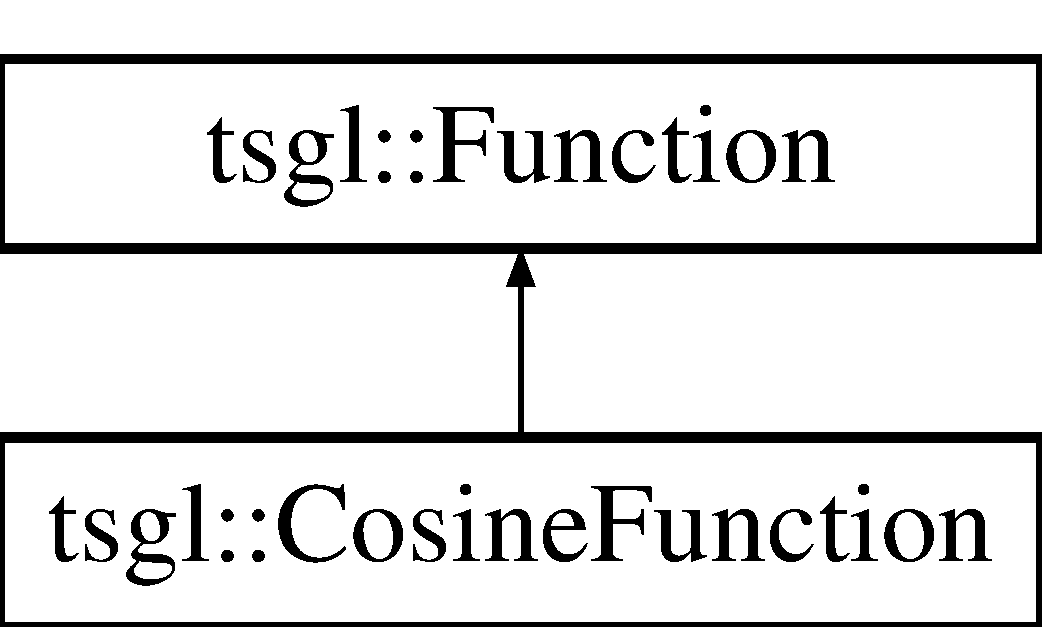
\includegraphics[height=2.000000cm]{classtsgl_1_1_cosine_function}
\end{center}
\end{figure}
\subsection*{Public Member Functions}
\begin{DoxyCompactItemize}
\item 
virtual Decimal \hyperlink{classtsgl_1_1_cosine_function_a69b67c247afe02895d35da9a99bc0ffd}{value\-At} (Decimal x) const 
\begin{DoxyCompactList}\small\item\em Method to determine the value of \hyperlink{classtsgl_1_1_cosine_function}{Cosine\-Function}. \end{DoxyCompactList}\end{DoxyCompactItemize}


\subsection{Detailed Description}
\hyperlink{classtsgl_1_1_function}{Function} to compute the cosine of the input. 

\subsection{Member Function Documentation}
\hypertarget{classtsgl_1_1_cosine_function_a69b67c247afe02895d35da9a99bc0ffd}{\index{tsgl\-::\-Cosine\-Function@{tsgl\-::\-Cosine\-Function}!value\-At@{value\-At}}
\index{value\-At@{value\-At}!tsgl::CosineFunction@{tsgl\-::\-Cosine\-Function}}
\subsubsection[{value\-At}]{\setlength{\rightskip}{0pt plus 5cm}virtual Decimal tsgl\-::\-Cosine\-Function\-::value\-At (
\begin{DoxyParamCaption}
\item[{Decimal}]{x}
\end{DoxyParamCaption}
) const\hspace{0.3cm}{\ttfamily [inline]}, {\ttfamily [virtual]}}}\label{classtsgl_1_1_cosine_function_a69b67c247afe02895d35da9a99bc0ffd}


Method to determine the value of \hyperlink{classtsgl_1_1_cosine_function}{Cosine\-Function}. 

\begin{DoxyReturn}{Returns}
The cosine of {\itshape x}. 
\end{DoxyReturn}


Implements \hyperlink{classtsgl_1_1_function_affb7b3b19a04efefa29a9870d666e912}{tsgl\-::\-Function}.



The documentation for this class was generated from the following file\-:\begin{DoxyCompactItemize}
\item 
Function.\-h\end{DoxyCompactItemize}

\hypertarget{classtsgl_1_1_exponential_function}{\section{tsgl\-:\-:Exponential\-Function Class Reference}
\label{classtsgl_1_1_exponential_function}\index{tsgl\-::\-Exponential\-Function@{tsgl\-::\-Exponential\-Function}}
}


\hyperlink{classtsgl_1_1_function}{Function} to compute e raised to the input.  




{\ttfamily \#include $<$Function.\-h$>$}

Inheritance diagram for tsgl\-:\-:Exponential\-Function\-:\begin{figure}[H]
\begin{center}
\leavevmode
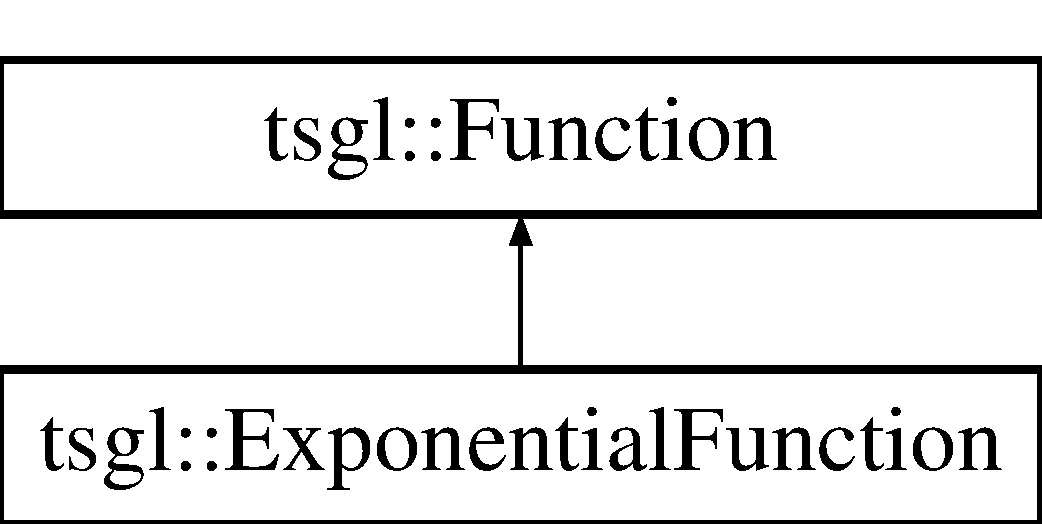
\includegraphics[height=2.000000cm]{classtsgl_1_1_exponential_function}
\end{center}
\end{figure}
\subsection*{Public Member Functions}
\begin{DoxyCompactItemize}
\item 
virtual Decimal \hyperlink{classtsgl_1_1_exponential_function_a059eae7c56a61c73b4c545b6c0e309d9}{value\-At} (Decimal x) const 
\begin{DoxyCompactList}\small\item\em Method to determine the value of \hyperlink{classtsgl_1_1_exponential_function}{Exponential\-Function}. \end{DoxyCompactList}\end{DoxyCompactItemize}


\subsection{Detailed Description}
\hyperlink{classtsgl_1_1_function}{Function} to compute e raised to the input. 

\subsection{Member Function Documentation}
\hypertarget{classtsgl_1_1_exponential_function_a059eae7c56a61c73b4c545b6c0e309d9}{\index{tsgl\-::\-Exponential\-Function@{tsgl\-::\-Exponential\-Function}!value\-At@{value\-At}}
\index{value\-At@{value\-At}!tsgl::ExponentialFunction@{tsgl\-::\-Exponential\-Function}}
\subsubsection[{value\-At}]{\setlength{\rightskip}{0pt plus 5cm}virtual Decimal tsgl\-::\-Exponential\-Function\-::value\-At (
\begin{DoxyParamCaption}
\item[{Decimal}]{x}
\end{DoxyParamCaption}
) const\hspace{0.3cm}{\ttfamily [inline]}, {\ttfamily [virtual]}}}\label{classtsgl_1_1_exponential_function_a059eae7c56a61c73b4c545b6c0e309d9}


Method to determine the value of \hyperlink{classtsgl_1_1_exponential_function}{Exponential\-Function}. 

\begin{DoxyReturn}{Returns}
{\itshape e} raised to the power of {\itshape x}. 
\end{DoxyReturn}


Implements \hyperlink{classtsgl_1_1_function_affb7b3b19a04efefa29a9870d666e912}{tsgl\-::\-Function}.



The documentation for this class was generated from the following file\-:\begin{DoxyCompactItemize}
\item 
Function.\-h\end{DoxyCompactItemize}

\hypertarget{classtsgl_1_1_floor_function}{}\section{tsgl\+:\+:Floor\+Function Class Reference}
\label{classtsgl_1_1_floor_function}\index{tsgl\+::\+Floor\+Function@{tsgl\+::\+Floor\+Function}}


\hyperlink{classtsgl_1_1_function}{Function} to compute the mathematical floor of the input.  




{\ttfamily \#include $<$Function.\+h$>$}

Inheritance diagram for tsgl\+:\+:Floor\+Function\+:\begin{figure}[H]
\begin{center}
\leavevmode
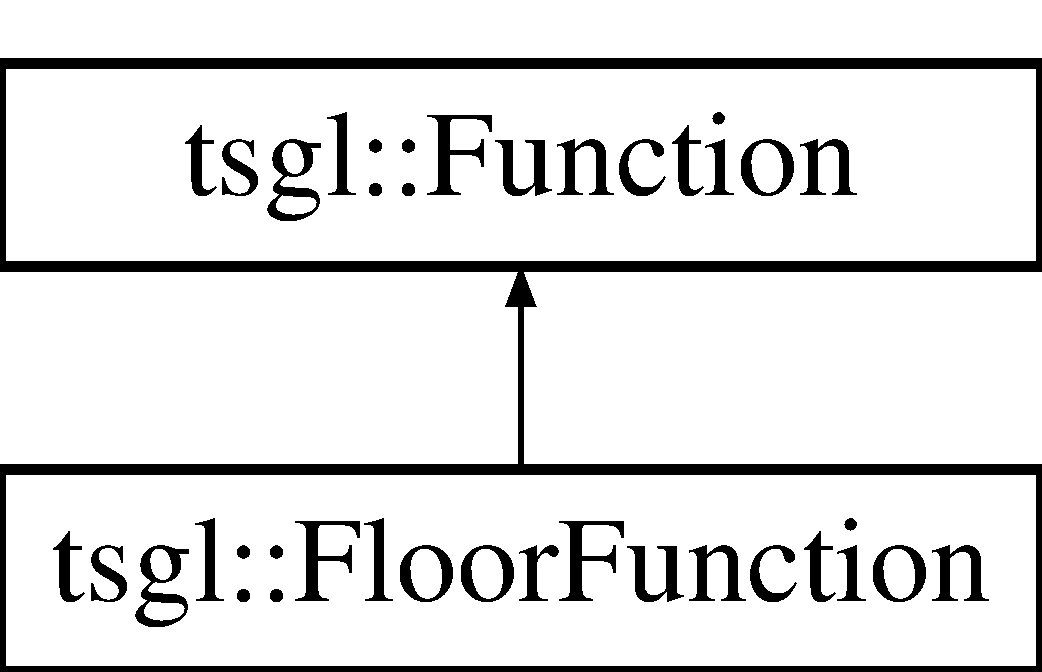
\includegraphics[height=2.000000cm]{classtsgl_1_1_floor_function}
\end{center}
\end{figure}
\subsection*{Public Member Functions}
\begin{DoxyCompactItemize}
\item 
virtual Decimal \hyperlink{classtsgl_1_1_floor_function_a73eedb6a65c55e070541b08c49d9f170}{value\+At} (Decimal x) const 
\begin{DoxyCompactList}\small\item\em Method to determine the value of \hyperlink{classtsgl_1_1_floor_function}{Floor\+Function}. \end{DoxyCompactList}\end{DoxyCompactItemize}


\subsection{Detailed Description}
\hyperlink{classtsgl_1_1_function}{Function} to compute the mathematical floor of the input. 

\subsection{Member Function Documentation}
\hypertarget{classtsgl_1_1_floor_function_a73eedb6a65c55e070541b08c49d9f170}{}\index{tsgl\+::\+Floor\+Function@{tsgl\+::\+Floor\+Function}!value\+At@{value\+At}}
\index{value\+At@{value\+At}!tsgl\+::\+Floor\+Function@{tsgl\+::\+Floor\+Function}}
\subsubsection[{value\+At}]{\setlength{\rightskip}{0pt plus 5cm}virtual Decimal tsgl\+::\+Floor\+Function\+::value\+At (
\begin{DoxyParamCaption}
\item[{Decimal}]{x}
\end{DoxyParamCaption}
) const\hspace{0.3cm}{\ttfamily [inline]}, {\ttfamily [virtual]}}\label{classtsgl_1_1_floor_function_a73eedb6a65c55e070541b08c49d9f170}


Method to determine the value of \hyperlink{classtsgl_1_1_floor_function}{Floor\+Function}. 

\begin{DoxyReturn}{Returns}
The largest integer less than or equal to {\itshape x}. 
\end{DoxyReturn}


Implements \hyperlink{classtsgl_1_1_function_affb7b3b19a04efefa29a9870d666e912}{tsgl\+::\+Function}.



The documentation for this class was generated from the following file\+:\begin{DoxyCompactItemize}
\item 
Function.\+h\end{DoxyCompactItemize}

\hypertarget{classtsgl_1_1_function}{\section{tsgl\-:\-:Function Class Reference}
\label{classtsgl_1_1_function}\index{tsgl\-::\-Function@{tsgl\-::\-Function}}
}


A base class for creating mathematical functions plottable by a \hyperlink{classtsgl_1_1_cartesian_canvas}{Cartesian\-Canvas}.  




{\ttfamily \#include $<$Function.\-h$>$}

Inheritance diagram for tsgl\-:\-:Function\-:\begin{figure}[H]
\begin{center}
\leavevmode
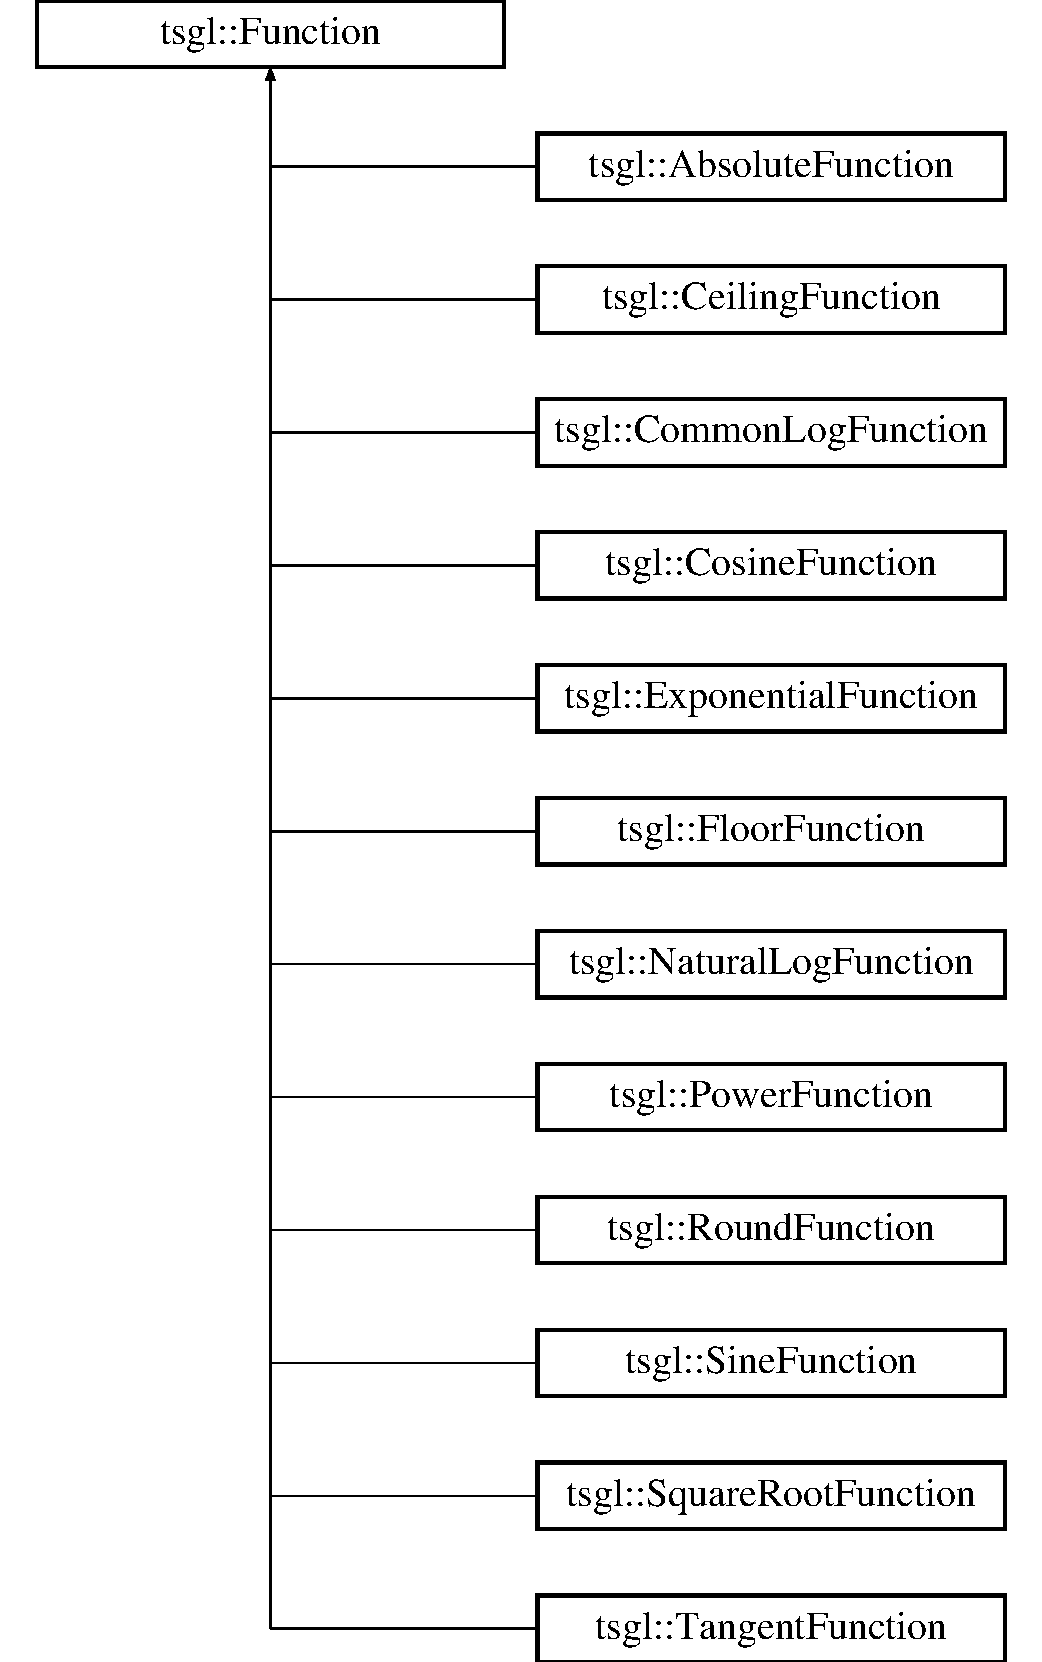
\includegraphics[height=12.000000cm]{classtsgl_1_1_function}
\end{center}
\end{figure}
\subsection*{Public Member Functions}
\begin{DoxyCompactItemize}
\item 
\hyperlink{classtsgl_1_1_function_aaf959c9d39bb45c2aded83fd754c288d}{Function} ()
\begin{DoxyCompactList}\small\item\em Constructs a new \hyperlink{classtsgl_1_1_function}{Function}. \end{DoxyCompactList}\item 
virtual \hyperlink{classtsgl_1_1_function_a3b8cbd26a32c6ae75b12e7397bb42c41}{$\sim$\-Function} ()
\begin{DoxyCompactList}\small\item\em Destructor for the \hyperlink{classtsgl_1_1_function}{Function} class. \end{DoxyCompactList}\item 
virtual Decimal \hyperlink{classtsgl_1_1_function_affb7b3b19a04efefa29a9870d666e912}{value\-At} (Decimal x) const =0
\begin{DoxyCompactList}\small\item\em Method to determine the value of a \hyperlink{classtsgl_1_1_function}{Function} subclass. \end{DoxyCompactList}\end{DoxyCompactItemize}


\subsection{Detailed Description}
A base class for creating mathematical functions plottable by a \hyperlink{classtsgl_1_1_cartesian_canvas}{Cartesian\-Canvas}. 

\hyperlink{classtsgl_1_1_function}{Function} provides a base class for the creation of mathematical functions. By extending this class and overriding the \hyperlink{classtsgl_1_1_function_affb7b3b19a04efefa29a9870d666e912}{value\-At()} method, users can easily plot the values of their function on a \hyperlink{classtsgl_1_1_cartesian_canvas}{Cartesian\-Canvas}.

A number of pre-\/built \hyperlink{classtsgl_1_1_function}{Function} subclasses are included in the header file for reference. 

\subsection{Constructor \& Destructor Documentation}
\hypertarget{classtsgl_1_1_function_aaf959c9d39bb45c2aded83fd754c288d}{\index{tsgl\-::\-Function@{tsgl\-::\-Function}!Function@{Function}}
\index{Function@{Function}!tsgl::Function@{tsgl\-::\-Function}}
\subsubsection[{Function}]{\setlength{\rightskip}{0pt plus 5cm}tsgl\-::\-Function\-::\-Function (
\begin{DoxyParamCaption}
{}
\end{DoxyParamCaption}
)\hspace{0.3cm}{\ttfamily [inline]}}}\label{classtsgl_1_1_function_aaf959c9d39bb45c2aded83fd754c288d}


Constructs a new \hyperlink{classtsgl_1_1_function}{Function}. 

This is the default constructor for the \hyperlink{classtsgl_1_1_function}{Function} class. \begin{DoxyNote}{Note}
The default constructor for the parent \hyperlink{classtsgl_1_1_function}{Function} class does absolutely nothing. Any construction should be defined in the subclass. 
\end{DoxyNote}
\hypertarget{classtsgl_1_1_function_a3b8cbd26a32c6ae75b12e7397bb42c41}{\index{tsgl\-::\-Function@{tsgl\-::\-Function}!$\sim$\-Function@{$\sim$\-Function}}
\index{$\sim$\-Function@{$\sim$\-Function}!tsgl::Function@{tsgl\-::\-Function}}
\subsubsection[{$\sim$\-Function}]{\setlength{\rightskip}{0pt plus 5cm}virtual tsgl\-::\-Function\-::$\sim$\-Function (
\begin{DoxyParamCaption}
{}
\end{DoxyParamCaption}
)\hspace{0.3cm}{\ttfamily [inline]}, {\ttfamily [virtual]}}}\label{classtsgl_1_1_function_a3b8cbd26a32c6ae75b12e7397bb42c41}


Destructor for the \hyperlink{classtsgl_1_1_function}{Function} class. 

\begin{DoxyNote}{Note}
The default destructor for the parent \hyperlink{classtsgl_1_1_function}{Function} class does absolutely nothing. Any destruction should be defined in the subclass. 
\end{DoxyNote}


\subsection{Member Function Documentation}
\hypertarget{classtsgl_1_1_function_affb7b3b19a04efefa29a9870d666e912}{\index{tsgl\-::\-Function@{tsgl\-::\-Function}!value\-At@{value\-At}}
\index{value\-At@{value\-At}!tsgl::Function@{tsgl\-::\-Function}}
\subsubsection[{value\-At}]{\setlength{\rightskip}{0pt plus 5cm}virtual Decimal tsgl\-::\-Function\-::value\-At (
\begin{DoxyParamCaption}
\item[{Decimal}]{x}
\end{DoxyParamCaption}
) const\hspace{0.3cm}{\ttfamily [pure virtual]}}}\label{classtsgl_1_1_function_affb7b3b19a04efefa29a9870d666e912}


Method to determine the value of a \hyperlink{classtsgl_1_1_function}{Function} subclass. 

This method should be overridden with the actual function you want to compute. 
\begin{DoxyParams}{Parameters}
{\em x} & The input to the function. Assuming your function is F, x will be used to compute F(x). \\
\hline
\end{DoxyParams}
\begin{DoxyReturn}{Returns}
The Decimal value of F(x). 
\end{DoxyReturn}
\begin{DoxyNote}{Note}
This method is abstract and {\bfseries must} be overridden. 
\end{DoxyNote}


Implemented in \hyperlink{classtsgl_1_1_round_function_a3047ee723fae828d9379d946012028ca}{tsgl\-::\-Round\-Function}, \hyperlink{classtsgl_1_1_floor_function_a73eedb6a65c55e070541b08c49d9f170}{tsgl\-::\-Floor\-Function}, \hyperlink{classtsgl_1_1_ceiling_function_ab47498860b2395e331f203c4025bcb81}{tsgl\-::\-Ceiling\-Function}, \hyperlink{classtsgl_1_1_common_log_function_ac320c0f57c0fc4801bf8eb85f07838d8}{tsgl\-::\-Common\-Log\-Function}, \hyperlink{classtsgl_1_1_natural_log_function_a21ce8c1cad8b13dccf9308c73a48df12}{tsgl\-::\-Natural\-Log\-Function}, \hyperlink{classtsgl_1_1_exponential_function_a059eae7c56a61c73b4c545b6c0e309d9}{tsgl\-::\-Exponential\-Function}, \hyperlink{classtsgl_1_1_absolute_function_a29b4dd051d17e92b4f2d64b492a6ca19}{tsgl\-::\-Absolute\-Function}, \hyperlink{classtsgl_1_1_tangent_function_a3737542399069ebce368a5b53ba8a563}{tsgl\-::\-Tangent\-Function}, \hyperlink{classtsgl_1_1_cosine_function_a69b67c247afe02895d35da9a99bc0ffd}{tsgl\-::\-Cosine\-Function}, \hyperlink{classtsgl_1_1_sine_function_a6507b049141d946ede1611050e44dab2}{tsgl\-::\-Sine\-Function}, \hyperlink{classtsgl_1_1_square_root_function_a25f6192ef7b12b80c4a14186e1cde97c}{tsgl\-::\-Square\-Root\-Function}, and \hyperlink{classtsgl_1_1_power_function_ae63821b4c2347508c42c300a0c306076}{tsgl\-::\-Power\-Function}.



The documentation for this class was generated from the following file\-:\begin{DoxyCompactItemize}
\item 
Function.\-h\end{DoxyCompactItemize}

\hypertarget{classtsgl_1_1_image}{\section{tsgl\-:\-:\-Image \-Class \-Reference}
\label{classtsgl_1_1_image}\index{tsgl\-::\-Image@{tsgl\-::\-Image}}
}


\-Draw an image to the \hyperlink{classtsgl_1_1_canvas}{\-Canvas}.  




{\ttfamily \#include $<$\-Image.\-h$>$}

\-Inheritance diagram for tsgl\-:\-:\-Image\-:\begin{figure}[H]
\begin{center}
\leavevmode
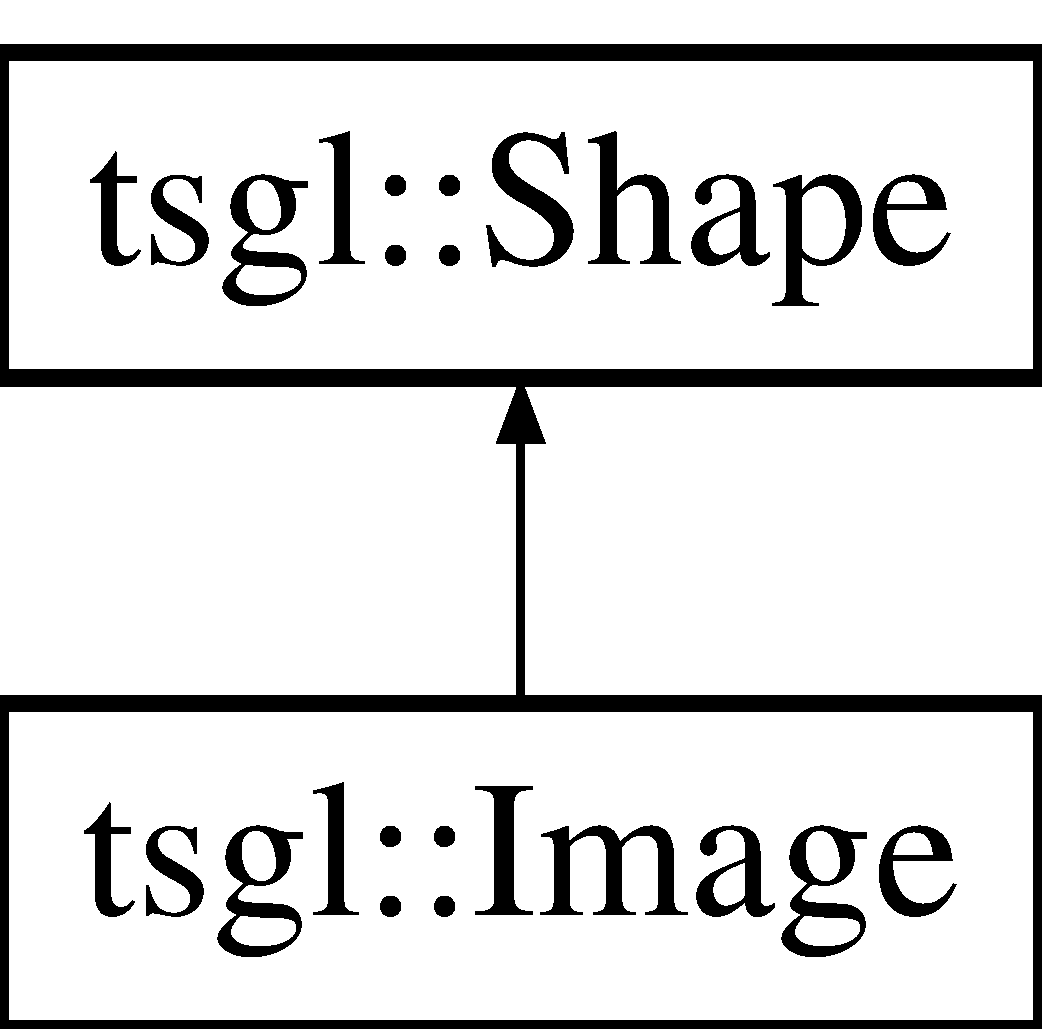
\includegraphics[height=2.000000cm]{classtsgl_1_1_image}
\end{center}
\end{figure}
\subsection*{\-Public \-Member \-Functions}
\begin{DoxyCompactItemize}
\item 
\hyperlink{classtsgl_1_1_image_a497894a4dbfa46d1e3aefd7dbe086cc3}{\-Image} (std\-::string filename, \hyperlink{classtsgl_1_1_texture_handler}{\-Texture\-Handler} \&loader, int x, int y, int width, int height, float alpha)
\begin{DoxyCompactList}\small\item\em \-Explicitly constructs a new \hyperlink{classtsgl_1_1_image}{\-Image}. \end{DoxyCompactList}\item 
void \hyperlink{classtsgl_1_1_image_a85732de312b98dd5ce5a9cc319bbf8c5}{draw} ()
\begin{DoxyCompactList}\small\item\em \-Draw the \hyperlink{classtsgl_1_1_image}{\-Image}. \end{DoxyCompactList}\item 
int \hyperlink{classtsgl_1_1_image_afa939262dcf32c9a504efe30a8de5c58}{get\-Height} ()
\begin{DoxyCompactList}\small\item\em \-Accessor for the image's height. \end{DoxyCompactList}\item 
int \hyperlink{classtsgl_1_1_image_af01d5f815b91f20fd441f9bcec671d79}{get\-Width} ()
\begin{DoxyCompactList}\small\item\em \-Accessor for the image's width. \end{DoxyCompactList}\end{DoxyCompactItemize}


\subsection{\-Detailed \-Description}
\-Draw an image to the \hyperlink{classtsgl_1_1_canvas}{\-Canvas}. 

\hyperlink{classtsgl_1_1_image}{\-Image} is a class which provides a simple interface for loading and drawing images. \-The \hyperlink{classtsgl_1_1_image}{\-Image} class currently supports files in the .png, .bmp, and .jpg formats. \begin{DoxyNote}{\-Note}
\-For the time being, there is no way to measure the size of an image once it's loaded. \-Therefore, the width and height must be specified manually, and stretching may occur if the input dimensions don't match the images actual dimensions. 

\-Additionally, an \-Image\-Loader must be passed as an argument. \-This \-Image\-Loader is automatically constructed with the \hyperlink{classtsgl_1_1_canvas}{\-Canvas} as the private $\ast$loader$\ast$ variable. \-At the moment, there is no way to extend \hyperlink{classtsgl_1_1_canvas_ae94a586629d20b7fabcb402d1c654628}{\-Canvas\-::draw\-Image()} function due to this privatization. 
\end{DoxyNote}
\begin{DoxyWarning}{\-Warning}
\-Aside from an error message output to stderr, \hyperlink{classtsgl_1_1_image}{\-Image} gives no indication if an image failed to load. 
\end{DoxyWarning}


\subsection{\-Constructor \& \-Destructor \-Documentation}
\hypertarget{classtsgl_1_1_image_a497894a4dbfa46d1e3aefd7dbe086cc3}{\index{tsgl\-::\-Image@{tsgl\-::\-Image}!\-Image@{\-Image}}
\index{\-Image@{\-Image}!tsgl::Image@{tsgl\-::\-Image}}
\subsubsection[{\-Image}]{\setlength{\rightskip}{0pt plus 5cm}{\bf tsgl\-::\-Image\-::\-Image} (
\begin{DoxyParamCaption}
\item[{std\-::string}]{filename, }
\item[{{\bf \-Texture\-Handler} \&}]{loader, }
\item[{int}]{x, }
\item[{int}]{y, }
\item[{int}]{width, }
\item[{int}]{height, }
\item[{float}]{alpha}
\end{DoxyParamCaption}
)}}\label{classtsgl_1_1_image_a497894a4dbfa46d1e3aefd7dbe086cc3}


\-Explicitly constructs a new \hyperlink{classtsgl_1_1_image}{\-Image}. 

\-This is the explicit constructor for the \hyperlink{classtsgl_1_1_image}{\-Image} class. 
\begin{DoxyParams}{\-Parameters}
{\em filename} & \-The filename of the image to load. \\
\hline
{\em loader} & \-A reference pointer to the \hyperlink{classtsgl_1_1_texture_handler}{\-Texture\-Handler} with which to load the image. \\
\hline
{\em x} & \-The x coordinate of the left of the \hyperlink{classtsgl_1_1_image}{\-Image}. \\
\hline
{\em y} & \-The y coordinate of the top of the \hyperlink{classtsgl_1_1_image}{\-Image}. \\
\hline
{\em width} & \-The width of the \hyperlink{classtsgl_1_1_image}{\-Image}. \\
\hline
{\em height} & \-The height of the \hyperlink{classtsgl_1_1_image}{\-Image}. \\
\hline
{\em alhpa} & \-The alpha of the \hyperlink{classtsgl_1_1_image}{\-Image}. \\
\hline
\end{DoxyParams}
\begin{DoxyReturn}{\-Returns}
\-A new \hyperlink{classtsgl_1_1_image}{\-Image} is drawn with the specified coordinates, dimensions, and transparency. 
\end{DoxyReturn}
\begin{DoxyNote}{\-Note}
{\bfseries \-I\-M\-P\-O\-R\-T\-A\-N\-T}\-: \-In \hyperlink{classtsgl_1_1_cartesian_canvas}{\-Cartesian\-Canvas}, $\ast$y$\ast$ specifies the bottom, not the top, of the image. 
\end{DoxyNote}


\subsection{\-Member \-Function \-Documentation}
\hypertarget{classtsgl_1_1_image_a85732de312b98dd5ce5a9cc319bbf8c5}{\index{tsgl\-::\-Image@{tsgl\-::\-Image}!draw@{draw}}
\index{draw@{draw}!tsgl::Image@{tsgl\-::\-Image}}
\subsubsection[{draw}]{\setlength{\rightskip}{0pt plus 5cm}void {\bf tsgl\-::\-Image\-::draw} (
\begin{DoxyParamCaption}
{}
\end{DoxyParamCaption}
)\hspace{0.3cm}{\ttfamily  \mbox{[}virtual\mbox{]}}}}\label{classtsgl_1_1_image_a85732de312b98dd5ce5a9cc319bbf8c5}


\-Draw the \hyperlink{classtsgl_1_1_image}{\-Image}. 

\-This function actually draws the \hyperlink{classtsgl_1_1_image}{\-Image} to the \hyperlink{classtsgl_1_1_canvas}{\-Canvas}. 

\-Implements \hyperlink{classtsgl_1_1_shape_af78b1627b97d621824ce86db214e2402}{tsgl\-::\-Shape}.

\hypertarget{classtsgl_1_1_image_afa939262dcf32c9a504efe30a8de5c58}{\index{tsgl\-::\-Image@{tsgl\-::\-Image}!get\-Height@{get\-Height}}
\index{get\-Height@{get\-Height}!tsgl::Image@{tsgl\-::\-Image}}
\subsubsection[{get\-Height}]{\setlength{\rightskip}{0pt plus 5cm}int {\bf tsgl\-::\-Image\-::get\-Height} (
\begin{DoxyParamCaption}
{}
\end{DoxyParamCaption}
)\hspace{0.3cm}{\ttfamily  \mbox{[}inline\mbox{]}}}}\label{classtsgl_1_1_image_afa939262dcf32c9a504efe30a8de5c58}


\-Accessor for the image's height. 

\begin{DoxyReturn}{\-Returns}
\-The height of the \hyperlink{classtsgl_1_1_image}{\-Image}. 
\end{DoxyReturn}
\hypertarget{classtsgl_1_1_image_af01d5f815b91f20fd441f9bcec671d79}{\index{tsgl\-::\-Image@{tsgl\-::\-Image}!get\-Width@{get\-Width}}
\index{get\-Width@{get\-Width}!tsgl::Image@{tsgl\-::\-Image}}
\subsubsection[{get\-Width}]{\setlength{\rightskip}{0pt plus 5cm}int {\bf tsgl\-::\-Image\-::get\-Width} (
\begin{DoxyParamCaption}
{}
\end{DoxyParamCaption}
)\hspace{0.3cm}{\ttfamily  \mbox{[}inline\mbox{]}}}}\label{classtsgl_1_1_image_af01d5f815b91f20fd441f9bcec671d79}


\-Accessor for the image's width. 

\begin{DoxyReturn}{\-Returns}
\-The width of the \hyperlink{classtsgl_1_1_image}{\-Image}. 
\end{DoxyReturn}


\-The documentation for this class was generated from the following files\-:\begin{DoxyCompactItemize}
\item 
\-Image.\-h\item 
\-Image.\-cpp\end{DoxyCompactItemize}

\hypertarget{classtsgl_1_1_integral_viewer}{\section{tsgl\-:\-:Integral\-Viewer Class Reference}
\label{classtsgl_1_1_integral_viewer}\index{tsgl\-::\-Integral\-Viewer@{tsgl\-::\-Integral\-Viewer}}
}


Provides a a tool for computing and visualizing integrals of functions.  




{\ttfamily \#include $<$Integral\-Viewer.\-h$>$}

\subsection*{Public Member Functions}
\begin{DoxyCompactItemize}
\item 
\hyperlink{classtsgl_1_1_integral_viewer_a1fe15a118865fcaf3067dc73cf3f912c}{Integral\-Viewer} (function\-Pointer f, int width, int height, Decimal start\-X, Decimal stop\-X, Decimal start\-Y=0, Decimal stop\-Y=1, std\-::string fname=\char`\"{}function\char`\"{})
\begin{DoxyCompactList}\small\item\em Default \hyperlink{classtsgl_1_1_integral_viewer}{Integral\-Viewer} constructor method. \end{DoxyCompactList}\item 
\hyperlink{classtsgl_1_1_integral_viewer_a50961f189bd1988fb9b96b66b701fdf2}{$\sim$\-Integral\-Viewer} ()
\begin{DoxyCompactList}\small\item\em \hyperlink{classtsgl_1_1_integral_viewer}{Integral\-Viewer} destructor method. \end{DoxyCompactList}\item 
double \hyperlink{classtsgl_1_1_integral_viewer_ab650c8790258ece715cd3e1f5c21a05a}{get\-Rec\-Time} () const 
\begin{DoxyCompactList}\small\item\em Accessor for the time the canvas spent integrating using the rectangle method. \end{DoxyCompactList}\item 
double \hyperlink{classtsgl_1_1_integral_viewer_a7dfb74deff1ca61873f2d897ca35309b}{get\-Trap\-Time} () const 
\begin{DoxyCompactList}\small\item\em Accessor for the time the canvas spent integrating using the trapezoid method. \end{DoxyCompactList}\item 
long double \hyperlink{classtsgl_1_1_integral_viewer_a213d814ac293686ecd06c45344fa242f}{rectangle\-Evaluate} (long long num\-Rectangles)
\begin{DoxyCompactList}\small\item\em Evaluate an integral using the rectangle method. \end{DoxyCompactList}\item 
long double \hyperlink{classtsgl_1_1_integral_viewer_a485bd58c87267460baf013cdf786eae7}{trapezoid\-Evaluate} (long long num\-Trapezoids)
\begin{DoxyCompactList}\small\item\em Evaluate an integral using the trapezoid method. \end{DoxyCompactList}\end{DoxyCompactItemize}


\subsection{Detailed Description}
Provides a a tool for computing and visualizing integrals of functions. 

\hyperlink{classtsgl_1_1_integral_viewer}{Integral\-Viewer} provides a simple interface for integrating functions and outputting the results of the integration, both numerically and visually. \hyperlink{classtsgl_1_1_integral_viewer}{Integral\-Viewer} can evaluate an arbitrary function of the type {\ttfamily Decimal my\-Function(\-Decimal x)}, where x is the input value of the function and the return value is the y value of the function. \hyperlink{classtsgl_1_1_integral_viewer}{Integral\-Viewer} can compute integrals using one or both of the rectangle method and the trapezoid method, and provides functions for displaying both on a custom \hyperlink{classtsgl_1_1_canvas}{Canvas}. Furthermore, these computations and visualizations are thread-\/safe; the number of threads to use can be set with {\ttfamily omp\-\_\-set\-\_\-num\-\_\-threads()}. 

\subsection{Constructor \& Destructor Documentation}
\hypertarget{classtsgl_1_1_integral_viewer_a1fe15a118865fcaf3067dc73cf3f912c}{\index{tsgl\-::\-Integral\-Viewer@{tsgl\-::\-Integral\-Viewer}!Integral\-Viewer@{Integral\-Viewer}}
\index{Integral\-Viewer@{Integral\-Viewer}!tsgl::IntegralViewer@{tsgl\-::\-Integral\-Viewer}}
\subsubsection[{Integral\-Viewer}]{\setlength{\rightskip}{0pt plus 5cm}tsgl\-::\-Integral\-Viewer\-::\-Integral\-Viewer (
\begin{DoxyParamCaption}
\item[{function\-Pointer}]{f, }
\item[{int}]{width, }
\item[{int}]{height, }
\item[{Decimal}]{start\-X, }
\item[{Decimal}]{stop\-X, }
\item[{Decimal}]{start\-Y = {\ttfamily 0}, }
\item[{Decimal}]{stop\-Y = {\ttfamily 1}, }
\item[{std\-::string}]{fname = {\ttfamily \char`\"{}function\char`\"{}}}
\end{DoxyParamCaption}
)}}\label{classtsgl_1_1_integral_viewer_a1fe15a118865fcaf3067dc73cf3f912c}


Default \hyperlink{classtsgl_1_1_integral_viewer}{Integral\-Viewer} constructor method. 

This is the default constructor for the \hyperlink{classtsgl_1_1_integral_viewer}{Integral\-Viewer} class. 
\begin{DoxyParams}{Parameters}
{\em f} & A function to integrate and display. The function must accept exactly one argument of type Decimal, and return a Decimal. \\
\hline
{\em width} & The width of the window displaying the integration. \\
\hline
{\em height} & The height of the window displaying the integration. \\
\hline
{\em start\-X} & The minimum x-\/value whose y-\/value should be computed. \\
\hline
{\em stop\-X} & The maximum x-\/value whose y-\/value should be computed. \\
\hline
{\em start\-Y} & The minimum y-\/value that should be displayed on the \hyperlink{classtsgl_1_1_integral_viewer}{Integral\-Viewer}'s \hyperlink{classtsgl_1_1_canvas}{Canvas}. \\
\hline
{\em stop\-Y} & The maximum y-\/value that should be displayed on the \hyperlink{classtsgl_1_1_integral_viewer}{Integral\-Viewer}'s \hyperlink{classtsgl_1_1_canvas}{Canvas}. \\
\hline
{\em fname} & A descriptive name for the function you wish to integrate. \\
\hline
\end{DoxyParams}
\begin{DoxyReturn}{Returns}
A new \hyperlink{classtsgl_1_1_integral_viewer}{Integral\-Viewer} with the specified dimensions, bounds, and function description. 
\end{DoxyReturn}
\hypertarget{classtsgl_1_1_integral_viewer_a50961f189bd1988fb9b96b66b701fdf2}{\index{tsgl\-::\-Integral\-Viewer@{tsgl\-::\-Integral\-Viewer}!$\sim$\-Integral\-Viewer@{$\sim$\-Integral\-Viewer}}
\index{$\sim$\-Integral\-Viewer@{$\sim$\-Integral\-Viewer}!tsgl::IntegralViewer@{tsgl\-::\-Integral\-Viewer}}
\subsubsection[{$\sim$\-Integral\-Viewer}]{\setlength{\rightskip}{0pt plus 5cm}tsgl\-::\-Integral\-Viewer\-::$\sim$\-Integral\-Viewer (
\begin{DoxyParamCaption}
{}
\end{DoxyParamCaption}
)}}\label{classtsgl_1_1_integral_viewer_a50961f189bd1988fb9b96b66b701fdf2}


\hyperlink{classtsgl_1_1_integral_viewer}{Integral\-Viewer} destructor method. 

This is the destructor for the \hyperlink{classtsgl_1_1_integral_viewer}{Integral\-Viewer} class.

Frees up memory that was allocated to a \hyperlink{classtsgl_1_1_integral_viewer}{Integral\-Viewer} instance. 

\subsection{Member Function Documentation}
\hypertarget{classtsgl_1_1_integral_viewer_ab650c8790258ece715cd3e1f5c21a05a}{\index{tsgl\-::\-Integral\-Viewer@{tsgl\-::\-Integral\-Viewer}!get\-Rec\-Time@{get\-Rec\-Time}}
\index{get\-Rec\-Time@{get\-Rec\-Time}!tsgl::IntegralViewer@{tsgl\-::\-Integral\-Viewer}}
\subsubsection[{get\-Rec\-Time}]{\setlength{\rightskip}{0pt plus 5cm}double tsgl\-::\-Integral\-Viewer\-::get\-Rec\-Time (
\begin{DoxyParamCaption}
{}
\end{DoxyParamCaption}
) const\hspace{0.3cm}{\ttfamily [inline]}}}\label{classtsgl_1_1_integral_viewer_ab650c8790258ece715cd3e1f5c21a05a}


Accessor for the time the canvas spent integrating using the rectangle method. 

\begin{DoxyReturn}{Returns}
The elapsed time in seconds for the integration using rectangles. 
\end{DoxyReturn}
\hypertarget{classtsgl_1_1_integral_viewer_a7dfb74deff1ca61873f2d897ca35309b}{\index{tsgl\-::\-Integral\-Viewer@{tsgl\-::\-Integral\-Viewer}!get\-Trap\-Time@{get\-Trap\-Time}}
\index{get\-Trap\-Time@{get\-Trap\-Time}!tsgl::IntegralViewer@{tsgl\-::\-Integral\-Viewer}}
\subsubsection[{get\-Trap\-Time}]{\setlength{\rightskip}{0pt plus 5cm}double tsgl\-::\-Integral\-Viewer\-::get\-Trap\-Time (
\begin{DoxyParamCaption}
{}
\end{DoxyParamCaption}
) const\hspace{0.3cm}{\ttfamily [inline]}}}\label{classtsgl_1_1_integral_viewer_a7dfb74deff1ca61873f2d897ca35309b}


Accessor for the time the canvas spent integrating using the trapezoid method. 

\begin{DoxyReturn}{Returns}
The elapsed time in seconds for the integration using trapezoids. 
\end{DoxyReturn}
\hypertarget{classtsgl_1_1_integral_viewer_a213d814ac293686ecd06c45344fa242f}{\index{tsgl\-::\-Integral\-Viewer@{tsgl\-::\-Integral\-Viewer}!rectangle\-Evaluate@{rectangle\-Evaluate}}
\index{rectangle\-Evaluate@{rectangle\-Evaluate}!tsgl::IntegralViewer@{tsgl\-::\-Integral\-Viewer}}
\subsubsection[{rectangle\-Evaluate}]{\setlength{\rightskip}{0pt plus 5cm}long double tsgl\-::\-Integral\-Viewer\-::rectangle\-Evaluate (
\begin{DoxyParamCaption}
\item[{long long}]{num\-Rectangles}
\end{DoxyParamCaption}
)}}\label{classtsgl_1_1_integral_viewer_a213d814ac293686ecd06c45344fa242f}


Evaluate an integral using the rectangle method. 


\begin{DoxyParams}{Parameters}
{\em num\-Rectangles} & The number of rectangles to use for the integration. \\
\hline
\end{DoxyParams}
\begin{DoxyReturn}{Returns}
The area under the curve represented by the \hyperlink{classtsgl_1_1_integral_viewer}{Integral\-Viewer}'s function, evaluated using the rectangle method. 
\end{DoxyReturn}
\hypertarget{classtsgl_1_1_integral_viewer_a485bd58c87267460baf013cdf786eae7}{\index{tsgl\-::\-Integral\-Viewer@{tsgl\-::\-Integral\-Viewer}!trapezoid\-Evaluate@{trapezoid\-Evaluate}}
\index{trapezoid\-Evaluate@{trapezoid\-Evaluate}!tsgl::IntegralViewer@{tsgl\-::\-Integral\-Viewer}}
\subsubsection[{trapezoid\-Evaluate}]{\setlength{\rightskip}{0pt plus 5cm}long double tsgl\-::\-Integral\-Viewer\-::trapezoid\-Evaluate (
\begin{DoxyParamCaption}
\item[{long long}]{num\-Trapezoids}
\end{DoxyParamCaption}
)}}\label{classtsgl_1_1_integral_viewer_a485bd58c87267460baf013cdf786eae7}


Evaluate an integral using the trapezoid method. 


\begin{DoxyParams}{Parameters}
{\em num\-Rectangles} & The number of trapezoids to use for the integration. \\
\hline
\end{DoxyParams}
\begin{DoxyReturn}{Returns}
The area under the curve represented by the \hyperlink{classtsgl_1_1_integral_viewer}{Integral\-Viewer}'s function, evaluated using the trapezoid method. 
\end{DoxyReturn}


The documentation for this class was generated from the following files\-:\begin{DoxyCompactItemize}
\item 
Integral\-Viewer.\-h\item 
Integral\-Viewer.\-cpp\end{DoxyCompactItemize}

\hypertarget{classtsgl_1_1_line}{\section{tsgl\-:\-:\-Line \-Class \-Reference}
\label{classtsgl_1_1_line}\index{tsgl\-::\-Line@{tsgl\-::\-Line}}
}


\-Draw a simple line.  




{\ttfamily \#include $<$\-Line.\-h$>$}

\-Inheritance diagram for tsgl\-:\-:\-Line\-:\begin{figure}[H]
\begin{center}
\leavevmode
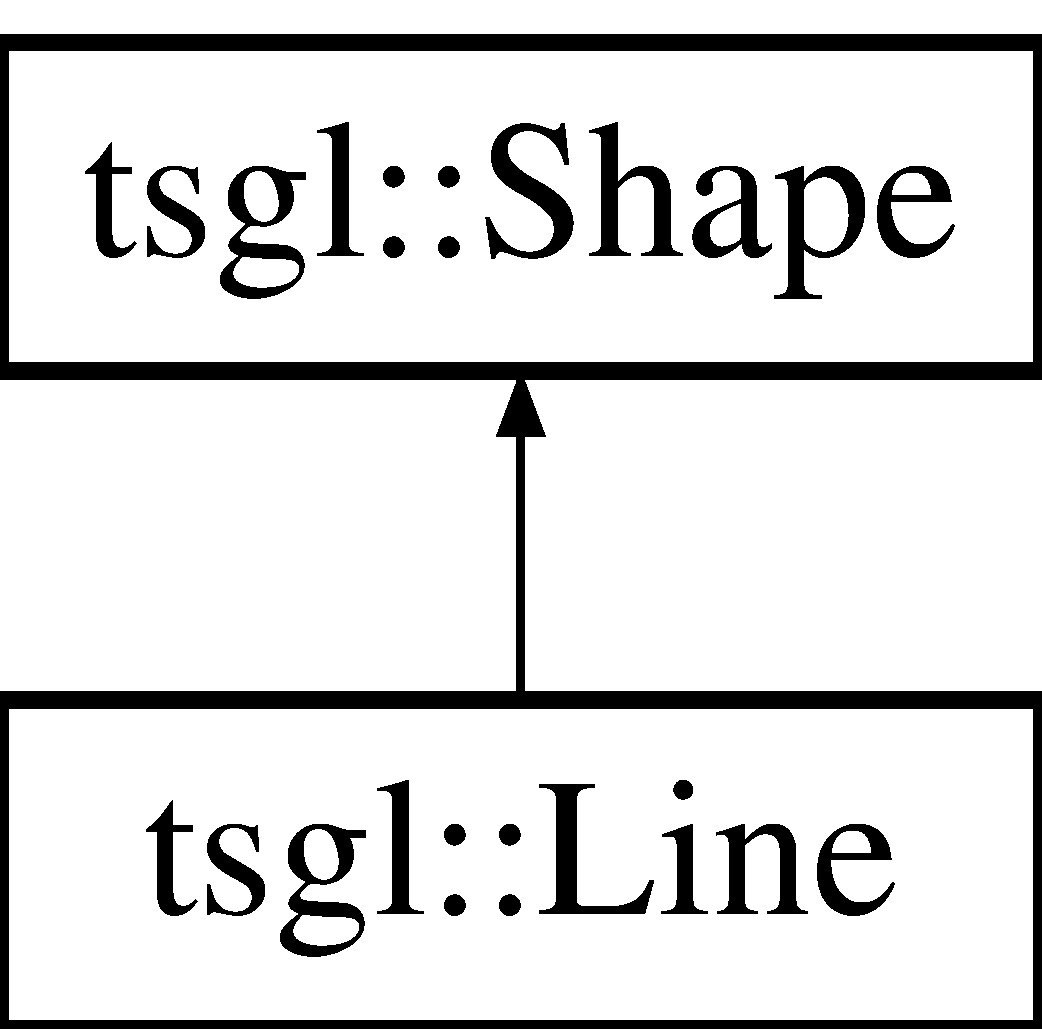
\includegraphics[height=2.000000cm]{classtsgl_1_1_line}
\end{center}
\end{figure}
\subsection*{\-Public \-Member \-Functions}
\begin{DoxyCompactItemize}
\item 
\hyperlink{classtsgl_1_1_line_af16488259ac5978679e13d58cf7e91ef}{\-Line} (int x1, int y1, int x2, int y2, const \hyperlink{structtsgl_1_1_color_float}{\-Color\-Float} \&color)
\begin{DoxyCompactList}\small\item\em \-Explicitly constructs a new \hyperlink{classtsgl_1_1_line}{\-Line}. \end{DoxyCompactList}\item 
void \hyperlink{classtsgl_1_1_line_ae7eccbbf5230a4c68139560d810af415}{draw} ()
\begin{DoxyCompactList}\small\item\em \-Draw the \hyperlink{classtsgl_1_1_line}{\-Line}. \end{DoxyCompactList}\end{DoxyCompactItemize}


\subsection{\-Detailed \-Description}
\-Draw a simple line. 

\hyperlink{classtsgl_1_1_line}{\-Line} is a class for holding vertex data for a simple line. 

\subsection{\-Constructor \& \-Destructor \-Documentation}
\hypertarget{classtsgl_1_1_line_af16488259ac5978679e13d58cf7e91ef}{\index{tsgl\-::\-Line@{tsgl\-::\-Line}!\-Line@{\-Line}}
\index{\-Line@{\-Line}!tsgl::Line@{tsgl\-::\-Line}}
\subsubsection[{\-Line}]{\setlength{\rightskip}{0pt plus 5cm}{\bf tsgl\-::\-Line\-::\-Line} (
\begin{DoxyParamCaption}
\item[{int}]{x1, }
\item[{int}]{y1, }
\item[{int}]{x2, }
\item[{int}]{y2, }
\item[{const {\bf \-Color\-Float} \&}]{color}
\end{DoxyParamCaption}
)}}\label{classtsgl_1_1_line_af16488259ac5978679e13d58cf7e91ef}


\-Explicitly constructs a new \hyperlink{classtsgl_1_1_line}{\-Line}. 

\-This is the constructor for the \hyperlink{classtsgl_1_1_line}{\-Line} class. 
\begin{DoxyParams}{\-Parameters}
{\em x1} & \-The x coordinate of the first endpoint. \\
\hline
{\em y1} & \-The y coordinate of the first endpoint. \\
\hline
{\em x2} & \-The x coordinate of the second endpoint. \\
\hline
{\em y2} & \-The y coordinate of the second endpoint. \\
\hline
{\em color} & \-The reference variable to the color of the \hyperlink{classtsgl_1_1_line}{\-Line}. \\
\hline
\end{DoxyParams}
\begin{DoxyReturn}{\-Returns}
\-A new \hyperlink{classtsgl_1_1_line}{\-Line} with the specified endpoints and color. 
\end{DoxyReturn}


\subsection{\-Member \-Function \-Documentation}
\hypertarget{classtsgl_1_1_line_ae7eccbbf5230a4c68139560d810af415}{\index{tsgl\-::\-Line@{tsgl\-::\-Line}!draw@{draw}}
\index{draw@{draw}!tsgl::Line@{tsgl\-::\-Line}}
\subsubsection[{draw}]{\setlength{\rightskip}{0pt plus 5cm}void {\bf tsgl\-::\-Line\-::draw} (
\begin{DoxyParamCaption}
{}
\end{DoxyParamCaption}
)\hspace{0.3cm}{\ttfamily  \mbox{[}virtual\mbox{]}}}}\label{classtsgl_1_1_line_ae7eccbbf5230a4c68139560d810af415}


\-Draw the \hyperlink{classtsgl_1_1_line}{\-Line}. 

\-This function actually draws the \hyperlink{classtsgl_1_1_line}{\-Line} to the \hyperlink{classtsgl_1_1_canvas}{\-Canvas}. 

\-Implements \hyperlink{classtsgl_1_1_shape_af78b1627b97d621824ce86db214e2402}{tsgl\-::\-Shape}.



\-The documentation for this class was generated from the following files\-:\begin{DoxyCompactItemize}
\item 
\-Line.\-h\item 
\-Line.\-cpp\end{DoxyCompactItemize}

\hypertarget{classtsgl_1_1_natural_log_function}{\section{tsgl\-:\-:\-Natural\-Log\-Function \-Class \-Reference}
\label{classtsgl_1_1_natural_log_function}\index{tsgl\-::\-Natural\-Log\-Function@{tsgl\-::\-Natural\-Log\-Function}}
}


\hyperlink{classtsgl_1_1_function}{\-Function} to compute the natural log of the input.  




{\ttfamily \#include $<$\-Function.\-h$>$}

\-Inheritance diagram for tsgl\-:\-:\-Natural\-Log\-Function\-:\begin{figure}[H]
\begin{center}
\leavevmode
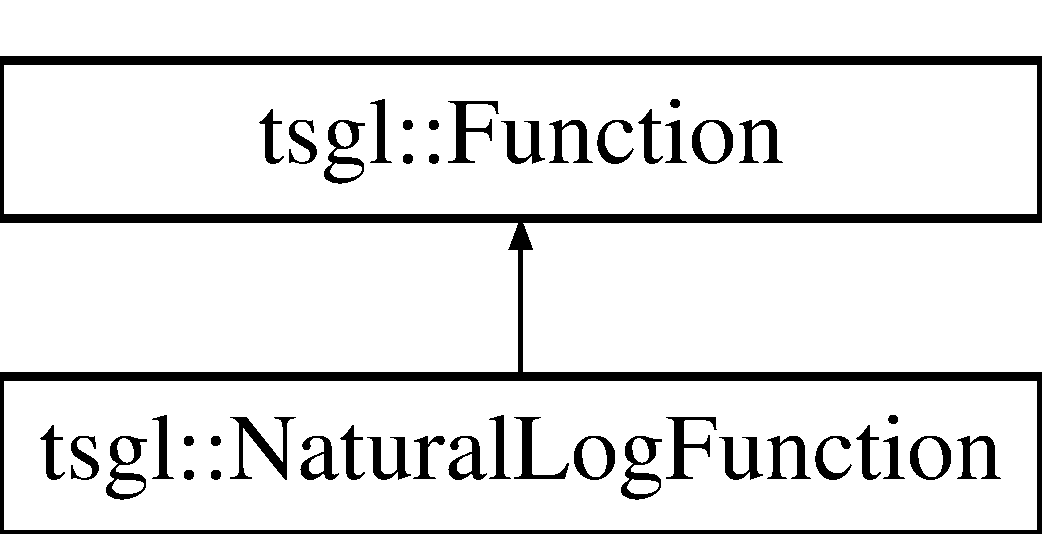
\includegraphics[height=2.000000cm]{classtsgl_1_1_natural_log_function}
\end{center}
\end{figure}
\subsection*{\-Public \-Member \-Functions}
\begin{DoxyCompactItemize}
\item 
virtual \-Decimal \hyperlink{classtsgl_1_1_natural_log_function_a21ce8c1cad8b13dccf9308c73a48df12}{value\-At} (\-Decimal x) const 
\begin{DoxyCompactList}\small\item\em \-Method to determine the value of \hyperlink{classtsgl_1_1_natural_log_function}{\-Natural\-Log\-Function}. \end{DoxyCompactList}\end{DoxyCompactItemize}


\subsection{\-Detailed \-Description}
\hyperlink{classtsgl_1_1_function}{\-Function} to compute the natural log of the input. 

\subsection{\-Member \-Function \-Documentation}
\hypertarget{classtsgl_1_1_natural_log_function_a21ce8c1cad8b13dccf9308c73a48df12}{\index{tsgl\-::\-Natural\-Log\-Function@{tsgl\-::\-Natural\-Log\-Function}!value\-At@{value\-At}}
\index{value\-At@{value\-At}!tsgl::NaturalLogFunction@{tsgl\-::\-Natural\-Log\-Function}}
\subsubsection[{value\-At}]{\setlength{\rightskip}{0pt plus 5cm}virtual \-Decimal {\bf tsgl\-::\-Natural\-Log\-Function\-::value\-At} (
\begin{DoxyParamCaption}
\item[{\-Decimal}]{x}
\end{DoxyParamCaption}
) const\hspace{0.3cm}{\ttfamily  \mbox{[}inline, virtual\mbox{]}}}}\label{classtsgl_1_1_natural_log_function_a21ce8c1cad8b13dccf9308c73a48df12}


\-Method to determine the value of \hyperlink{classtsgl_1_1_natural_log_function}{\-Natural\-Log\-Function}. 

\begin{DoxyReturn}{\-Returns}
\-The natural log of $\ast$x$\ast$. 
\end{DoxyReturn}


\-Implements \hyperlink{classtsgl_1_1_function_affb7b3b19a04efefa29a9870d666e912}{tsgl\-::\-Function}.



\-The documentation for this class was generated from the following file\-:\begin{DoxyCompactItemize}
\item 
\-Function.\-h\end{DoxyCompactItemize}

\hypertarget{classtsgl_1_1_polyline}{\section{tsgl\-:\-:\-Polyline \-Class \-Reference}
\label{classtsgl_1_1_polyline}\index{tsgl\-::\-Polyline@{tsgl\-::\-Polyline}}
}


\-Draw multiple lines chained together.  




{\ttfamily \#include $<$\-Polyline.\-h$>$}

\-Inheritance diagram for tsgl\-:\-:\-Polyline\-:\begin{figure}[H]
\begin{center}
\leavevmode
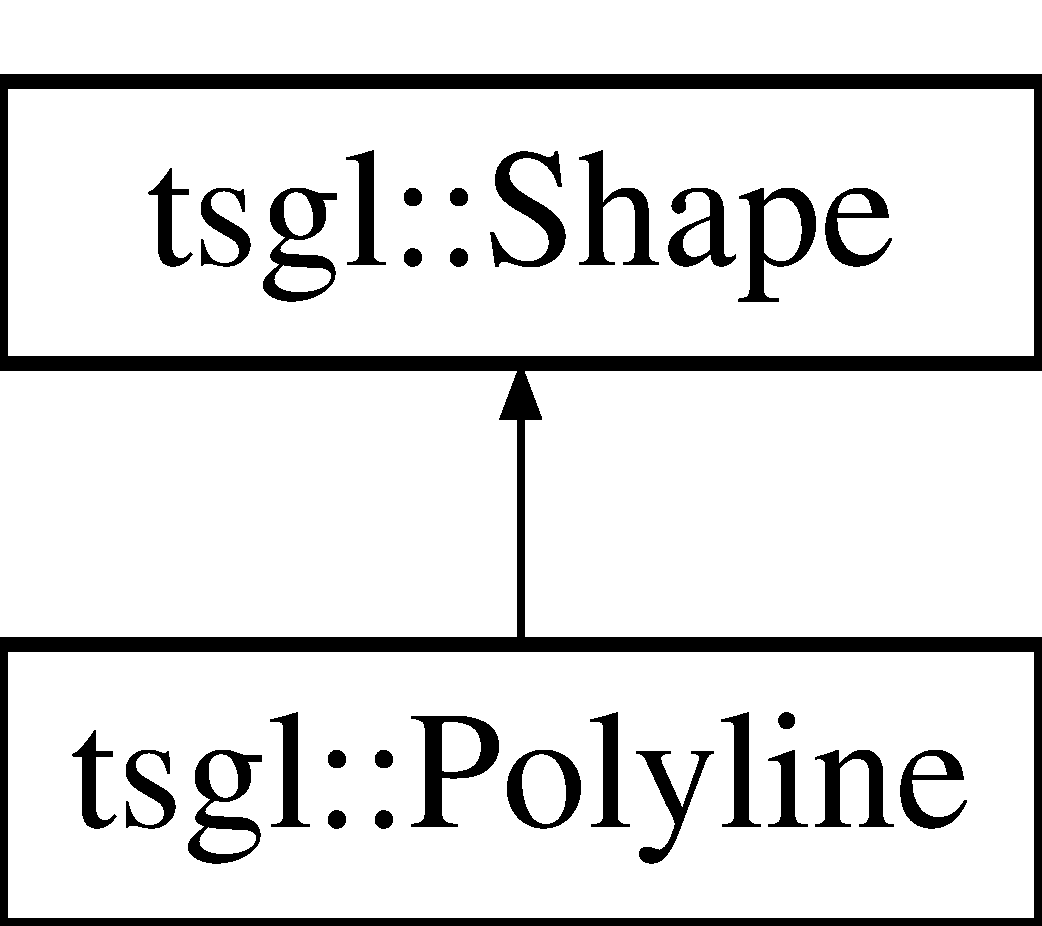
\includegraphics[height=2.000000cm]{classtsgl_1_1_polyline}
\end{center}
\end{figure}
\subsection*{\-Public \-Member \-Functions}
\begin{DoxyCompactItemize}
\item 
\hyperlink{classtsgl_1_1_polyline_ac618ba8a40d1f8fee9247264dc5e7513}{\-Polyline} (int num\-Vertices)
\begin{DoxyCompactList}\small\item\em \-Explicitly constructs a new \hyperlink{classtsgl_1_1_polyline}{\-Polyline}. \end{DoxyCompactList}\item 
\hyperlink{classtsgl_1_1_polyline_a5e186f8a65dae833d123480552b0eaad}{$\sim$\-Polyline} ()
\begin{DoxyCompactList}\small\item\em \-Destroys a \hyperlink{classtsgl_1_1_polyline}{\-Polyline} object. \end{DoxyCompactList}\item 
void \hyperlink{classtsgl_1_1_polyline_ab6598c7f60e57d9b988b19e90123da53}{add\-Next\-Vertex} (int x, int y, const \hyperlink{structtsgl_1_1_color_float}{\-Color\-Float} \&color=\-B\-L\-A\-C\-K)
\begin{DoxyCompactList}\small\item\em \-Adds another vertex to a \hyperlink{classtsgl_1_1_polyline}{\-Polyline}. \end{DoxyCompactList}\item 
void \hyperlink{classtsgl_1_1_polyline_ac6de5e2817824d9427d02d3e7be37f47}{draw} ()
\begin{DoxyCompactList}\small\item\em \-Draw the \hyperlink{classtsgl_1_1_polyline}{\-Polyline}. \end{DoxyCompactList}\end{DoxyCompactItemize}


\subsection{\-Detailed \-Description}
\-Draw multiple lines chained together. 

\hyperlink{classtsgl_1_1_polyline}{\-Polyline} is a class for holding vertex data for multiple lines whose endpoints are connected.

\-This method is optimized for long lists and offers a marked improvement over drawing individual \hyperlink{classtsgl_1_1_line}{\-Line} instances. \begin{DoxyNote}{\-Note}
\-The add\-Vertex() method must be called the same number of times as specified in the constructor. 

\-Calling add\-Vertex() after all vertices have been added will do nothing. 

\-Calling \hyperlink{classtsgl_1_1_polyline_ac6de5e2817824d9427d02d3e7be37f47}{draw()} before all vertices have been added will do nothing. 
\end{DoxyNote}


\subsection{\-Constructor \& \-Destructor \-Documentation}
\hypertarget{classtsgl_1_1_polyline_ac618ba8a40d1f8fee9247264dc5e7513}{\index{tsgl\-::\-Polyline@{tsgl\-::\-Polyline}!\-Polyline@{\-Polyline}}
\index{\-Polyline@{\-Polyline}!tsgl::Polyline@{tsgl\-::\-Polyline}}
\subsubsection[{\-Polyline}]{\setlength{\rightskip}{0pt plus 5cm}{\bf tsgl\-::\-Polyline\-::\-Polyline} (
\begin{DoxyParamCaption}
\item[{int}]{num\-Vertices}
\end{DoxyParamCaption}
)}}\label{classtsgl_1_1_polyline_ac618ba8a40d1f8fee9247264dc5e7513}


\-Explicitly constructs a new \hyperlink{classtsgl_1_1_polyline}{\-Polyline}. 

\-Explicit constructor for a new \hyperlink{classtsgl_1_1_polyline}{\-Polyline} object. 
\begin{DoxyParams}{\-Parameters}
{\em num\-Vertices} & \-The number of vertices the complete \hyperlink{classtsgl_1_1_polyline}{\-Polyline} will have. \\
\hline
\end{DoxyParams}
\begin{DoxyWarning}{\-Warning}
\-An invariant is held where if v is less than 2 then an error message is given. 
\end{DoxyWarning}
\begin{DoxyReturn}{\-Returns}
\-A new \hyperlink{classtsgl_1_1_polyline}{\-Polyline} with a buffer for storing the specified numbered of vertices. 
\end{DoxyReturn}
\hypertarget{classtsgl_1_1_polyline_a5e186f8a65dae833d123480552b0eaad}{\index{tsgl\-::\-Polyline@{tsgl\-::\-Polyline}!$\sim$\-Polyline@{$\sim$\-Polyline}}
\index{$\sim$\-Polyline@{$\sim$\-Polyline}!tsgl::Polyline@{tsgl\-::\-Polyline}}
\subsubsection[{$\sim$\-Polyline}]{\setlength{\rightskip}{0pt plus 5cm}{\bf tsgl\-::\-Polyline\-::$\sim$\-Polyline} (
\begin{DoxyParamCaption}
{}
\end{DoxyParamCaption}
)}}\label{classtsgl_1_1_polyline_a5e186f8a65dae833d123480552b0eaad}


\-Destroys a \hyperlink{classtsgl_1_1_polyline}{\-Polyline} object. 

\-Destructor for a \hyperlink{classtsgl_1_1_polyline}{\-Polyline} object.

\-Frees up memory allocated to a \hyperlink{classtsgl_1_1_polyline}{\-Polyline} object. 

\subsection{\-Member \-Function \-Documentation}
\hypertarget{classtsgl_1_1_polyline_ab6598c7f60e57d9b988b19e90123da53}{\index{tsgl\-::\-Polyline@{tsgl\-::\-Polyline}!add\-Next\-Vertex@{add\-Next\-Vertex}}
\index{add\-Next\-Vertex@{add\-Next\-Vertex}!tsgl::Polyline@{tsgl\-::\-Polyline}}
\subsubsection[{add\-Next\-Vertex}]{\setlength{\rightskip}{0pt plus 5cm}void {\bf tsgl\-::\-Polyline\-::add\-Next\-Vertex} (
\begin{DoxyParamCaption}
\item[{int}]{x, }
\item[{int}]{y, }
\item[{const {\bf \-Color\-Float} \&}]{color = {\ttfamily \-B\-L\-A\-C\-K}}
\end{DoxyParamCaption}
)}}\label{classtsgl_1_1_polyline_ab6598c7f60e57d9b988b19e90123da53}


\-Adds another vertex to a \hyperlink{classtsgl_1_1_polyline}{\-Polyline}. 

\-This function initializes the next vertex in a \hyperlink{classtsgl_1_1_polyline}{\-Polyline} and adds it to the \hyperlink{classtsgl_1_1_polyline}{\-Polyline}'s buffer. 
\begin{DoxyParams}{\-Parameters}
{\em x} & \-The x position of the vertex. \\
\hline
{\em y} & \-The y position of the vertex. \\
\hline
{\em color} & \-The reference variable to the color of the vertex (set to \-B\-L\-A\-C\-K by default). \\
\hline
\end{DoxyParams}
\begin{DoxyNote}{\-Note}
\-This function does nothing if the vertex buffer is already full. 

\-A message is given indicating when the vertex buffer is full. 
\end{DoxyNote}


\-Referenced by tsgl\-::\-Canvas\-::draw\-Circle(), tsgl\-::\-Canvas\-::draw\-Concave\-Polygon(), tsgl\-::\-Canvas\-::draw\-Convex\-Polygon(), tsgl\-::\-Cartesian\-Canvas\-::draw\-Function(), tsgl\-::\-Cartesian\-Canvas\-::draw\-Partial\-Function(), tsgl\-::\-Canvas\-::draw\-Rectangle(), tsgl\-::\-Canvas\-::draw\-Triangle(), tsgl\-::\-Canvas\-::draw\-Triangle\-Strip(), and tsgl\-::\-Progress\-Bar\-::get\-Border().

\hypertarget{classtsgl_1_1_polyline_ac6de5e2817824d9427d02d3e7be37f47}{\index{tsgl\-::\-Polyline@{tsgl\-::\-Polyline}!draw@{draw}}
\index{draw@{draw}!tsgl::Polyline@{tsgl\-::\-Polyline}}
\subsubsection[{draw}]{\setlength{\rightskip}{0pt plus 5cm}void {\bf tsgl\-::\-Polyline\-::draw} (
\begin{DoxyParamCaption}
{}
\end{DoxyParamCaption}
)\hspace{0.3cm}{\ttfamily  \mbox{[}virtual\mbox{]}}}}\label{classtsgl_1_1_polyline_ac6de5e2817824d9427d02d3e7be37f47}


\-Draw the \hyperlink{classtsgl_1_1_polyline}{\-Polyline}. 

\-This function actually draws the \hyperlink{classtsgl_1_1_polyline}{\-Polyline} to the \hyperlink{classtsgl_1_1_canvas}{\-Canvas}. \begin{DoxyNote}{\-Note}
\-This function does nothing if the vertex buffer is not yet full. 

\-A message indicating that the \hyperlink{classtsgl_1_1_polyline}{\-Polyline} cannot be drawn yet will be given if the above condition is met (vertex buffer = not full). 
\end{DoxyNote}


\-Implements \hyperlink{classtsgl_1_1_shape_af78b1627b97d621824ce86db214e2402}{tsgl\-::\-Shape}.



\-The documentation for this class was generated from the following files\-:\begin{DoxyCompactItemize}
\item 
\-Polyline.\-h\item 
\-Polyline.\-cpp\end{DoxyCompactItemize}

\hypertarget{classtsgl_1_1_power_function}{}\section{tsgl\+:\+:Power\+Function Class Reference}
\label{classtsgl_1_1_power_function}\index{tsgl\+::\+Power\+Function@{tsgl\+::\+Power\+Function}}


\hyperlink{classtsgl_1_1_function}{Function} to compute the input raised to a specified power.  




{\ttfamily \#include $<$Function.\+h$>$}

Inheritance diagram for tsgl\+:\+:Power\+Function\+:\begin{figure}[H]
\begin{center}
\leavevmode
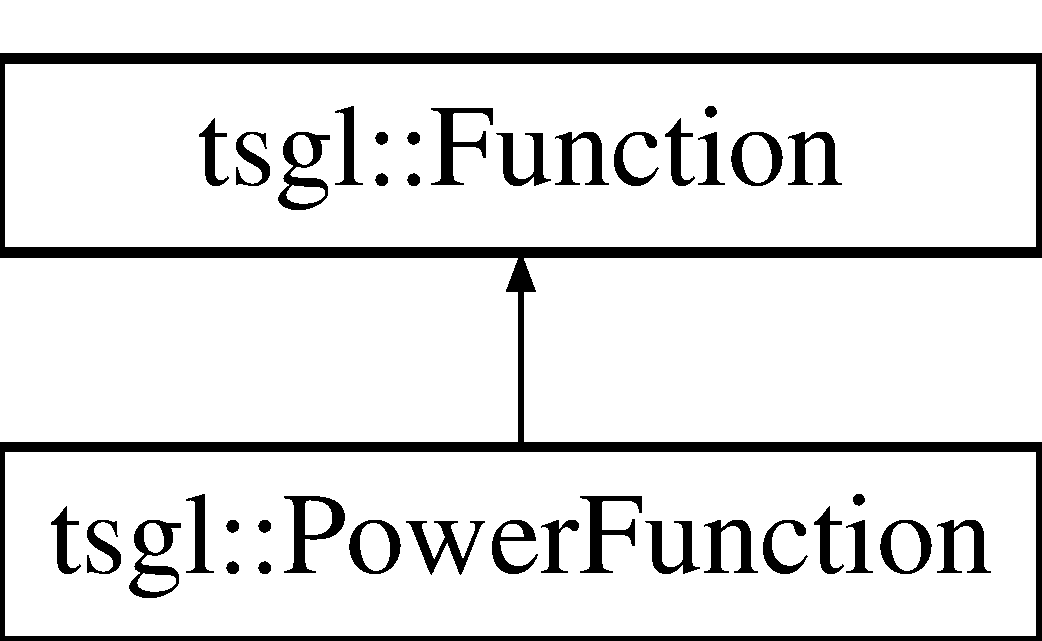
\includegraphics[height=2.000000cm]{classtsgl_1_1_power_function}
\end{center}
\end{figure}
\subsection*{Public Member Functions}
\begin{DoxyCompactItemize}
\item 
\hyperlink{classtsgl_1_1_power_function_a0a5d692e9bc9cf2a176ecab4ffc06519}{Power\+Function} (Decimal a)
\begin{DoxyCompactList}\small\item\em Constructs a new \hyperlink{classtsgl_1_1_power_function}{Power\+Function}. \end{DoxyCompactList}\item 
virtual Decimal \hyperlink{classtsgl_1_1_power_function_ae63821b4c2347508c42c300a0c306076}{value\+At} (Decimal x) const 
\begin{DoxyCompactList}\small\item\em Method to determine the value of \hyperlink{classtsgl_1_1_power_function}{Power\+Function}. \end{DoxyCompactList}\end{DoxyCompactItemize}


\subsection{Detailed Description}
\hyperlink{classtsgl_1_1_function}{Function} to compute the input raised to a specified power. 

\subsection{Constructor \& Destructor Documentation}
\hypertarget{classtsgl_1_1_power_function_a0a5d692e9bc9cf2a176ecab4ffc06519}{}\index{tsgl\+::\+Power\+Function@{tsgl\+::\+Power\+Function}!Power\+Function@{Power\+Function}}
\index{Power\+Function@{Power\+Function}!tsgl\+::\+Power\+Function@{tsgl\+::\+Power\+Function}}
\subsubsection[{Power\+Function}]{\setlength{\rightskip}{0pt plus 5cm}tsgl\+::\+Power\+Function\+::\+Power\+Function (
\begin{DoxyParamCaption}
\item[{Decimal}]{a}
\end{DoxyParamCaption}
)\hspace{0.3cm}{\ttfamily [inline]}}\label{classtsgl_1_1_power_function_a0a5d692e9bc9cf2a176ecab4ffc06519}


Constructs a new \hyperlink{classtsgl_1_1_power_function}{Power\+Function}. 


\begin{DoxyParams}{Parameters}
{\em a} & The power to which the input is raised. \\
\hline
\end{DoxyParams}


\subsection{Member Function Documentation}
\hypertarget{classtsgl_1_1_power_function_ae63821b4c2347508c42c300a0c306076}{}\index{tsgl\+::\+Power\+Function@{tsgl\+::\+Power\+Function}!value\+At@{value\+At}}
\index{value\+At@{value\+At}!tsgl\+::\+Power\+Function@{tsgl\+::\+Power\+Function}}
\subsubsection[{value\+At}]{\setlength{\rightskip}{0pt plus 5cm}virtual Decimal tsgl\+::\+Power\+Function\+::value\+At (
\begin{DoxyParamCaption}
\item[{Decimal}]{x}
\end{DoxyParamCaption}
) const\hspace{0.3cm}{\ttfamily [inline]}, {\ttfamily [virtual]}}\label{classtsgl_1_1_power_function_ae63821b4c2347508c42c300a0c306076}


Method to determine the value of \hyperlink{classtsgl_1_1_power_function}{Power\+Function}. 


\begin{DoxyParams}{Parameters}
{\em x} & The input to the function. \\
\hline
\end{DoxyParams}
\begin{DoxyReturn}{Returns}
{\itshape x} raised to the $\ast$a$\ast$th power. 
\end{DoxyReturn}


Implements \hyperlink{classtsgl_1_1_function_affb7b3b19a04efefa29a9870d666e912}{tsgl\+::\+Function}.



The documentation for this class was generated from the following file\+:\begin{DoxyCompactItemize}
\item 
Function.\+h\end{DoxyCompactItemize}

\hypertarget{classtsgl_1_1_progress_bar}{}\section{tsgl\+:\+:Progress\+Bar Class Reference}
\label{classtsgl_1_1_progress_bar}\index{tsgl\+::\+Progress\+Bar@{tsgl\+::\+Progress\+Bar}}


Draws and updates a progress bar.  




{\ttfamily \#include $<$Progress\+Bar.\+h$>$}

\subsection*{Public Member Functions}
\begin{DoxyCompactItemize}
\item 
\hyperlink{classtsgl_1_1_progress_bar_ac79018d09a75c490de3490306146c010}{Progress\+Bar} (int x, int y, int width, int height, float min\+Value, float max\+Value, unsigned num\+Segments)
\begin{DoxyCompactList}\small\item\em Explicit \hyperlink{classtsgl_1_1_progress_bar}{Progress\+Bar} constructor method. \end{DoxyCompactList}\item 
\hyperlink{classtsgl_1_1_progress_bar_aa3ad600db2cbd0e8f9221c264535df21}{$\sim$\+Progress\+Bar} ()
\begin{DoxyCompactList}\small\item\em \hyperlink{classtsgl_1_1_progress_bar}{Progress\+Bar} destructor method. \end{DoxyCompactList}\item 
void \hyperlink{classtsgl_1_1_progress_bar_a4274998e4935f33eb9212b2174d9c0c5}{update} (float new\+Value, int segnum=-\/1)
\begin{DoxyCompactList}\small\item\em Updates a \hyperlink{classtsgl_1_1_progress_bar}{Progress\+Bar} segment with a new value. \end{DoxyCompactList}\item 
\hyperlink{classtsgl_1_1_polyline}{Polyline} $\ast$ \hyperlink{classtsgl_1_1_progress_bar_ac2b51bdb0d19afaa03d60a9928fc873f}{get\+Border} (int index)
\begin{DoxyCompactList}\small\item\em Accessor for the \hyperlink{classtsgl_1_1_progress_bar}{Progress\+Bar}\textquotesingle{}s representative \hyperlink{classtsgl_1_1_polyline}{Polyline} array. \end{DoxyCompactList}\item 
\hyperlink{classtsgl_1_1_rectangle}{Rectangle} $\ast$ \hyperlink{classtsgl_1_1_progress_bar_aa360099f70e0c33c99f349cf28cbe610}{get\+Rect} (int index)
\begin{DoxyCompactList}\small\item\em Accessor for the \hyperlink{classtsgl_1_1_progress_bar}{Progress\+Bar}\textquotesingle{}s representative \hyperlink{classtsgl_1_1_rectangle}{Rectangle} array. \end{DoxyCompactList}\item 
int \hyperlink{classtsgl_1_1_progress_bar_a25576903783f18f8d74570aed2f80d95}{get\+Segs} ()
\begin{DoxyCompactList}\small\item\em Accessor for the \hyperlink{classtsgl_1_1_progress_bar}{Progress\+Bar}\textquotesingle{}s number of segments. \end{DoxyCompactList}\item 
int \hyperlink{classtsgl_1_1_progress_bar_a7ecdc35e44496db7cf2e25b2ee6577d4}{get\+Seg\+X} (int i)
\begin{DoxyCompactList}\small\item\em Accessor for a segment\textquotesingle{}s x position. \end{DoxyCompactList}\item 
int \hyperlink{classtsgl_1_1_progress_bar_a7efb6be08196ad2b48d4417a93d750ad}{get\+Seg\+Y} ()
\begin{DoxyCompactList}\small\item\em Accessor for a segment\textquotesingle{}s y position. \end{DoxyCompactList}\end{DoxyCompactItemize}


\subsection{Detailed Description}
Draws and updates a progress bar. 

\hyperlink{classtsgl_1_1_progress_bar}{Progress\+Bar} is a class for holding vertex data for multiple rectangles forming a progress bar. \hyperlink{classtsgl_1_1_progress_bar}{Progress\+Bar} is formed of multiple segments, each of which is thread-\/safe and updated individually with the \hyperlink{classtsgl_1_1_progress_bar_a4274998e4935f33eb9212b2174d9c0c5}{update()} method. A \hyperlink{classtsgl_1_1_progress_bar}{Progress\+Bar} can be drawn to the screen using \hyperlink{classtsgl_1_1_canvas_aea792059486ebe6d25d7f81bdadf751d}{Canvas\+::draw\+Progress()}. 

\subsection{Constructor \& Destructor Documentation}
\hypertarget{classtsgl_1_1_progress_bar_ac79018d09a75c490de3490306146c010}{}\index{tsgl\+::\+Progress\+Bar@{tsgl\+::\+Progress\+Bar}!Progress\+Bar@{Progress\+Bar}}
\index{Progress\+Bar@{Progress\+Bar}!tsgl\+::\+Progress\+Bar@{tsgl\+::\+Progress\+Bar}}
\subsubsection[{Progress\+Bar}]{\setlength{\rightskip}{0pt plus 5cm}tsgl\+::\+Progress\+Bar\+::\+Progress\+Bar (
\begin{DoxyParamCaption}
\item[{int}]{x, }
\item[{int}]{y, }
\item[{int}]{width, }
\item[{int}]{height, }
\item[{float}]{min\+Value, }
\item[{float}]{max\+Value, }
\item[{unsigned}]{num\+Segments}
\end{DoxyParamCaption}
)}\label{classtsgl_1_1_progress_bar_ac79018d09a75c490de3490306146c010}


Explicit \hyperlink{classtsgl_1_1_progress_bar}{Progress\+Bar} constructor method. 

This is the explicit constructor for the \hyperlink{classtsgl_1_1_progress_bar}{Progress\+Bar} class. 
\begin{DoxyParams}{Parameters}
{\em x} & The x position of the left edge of the \hyperlink{classtsgl_1_1_progress_bar}{Progress\+Bar}. \\
\hline
{\em y} & The y position of the top edge of the \hyperlink{classtsgl_1_1_progress_bar}{Progress\+Bar}. \\
\hline
{\em width} & The maximum width in pixels of the \hyperlink{classtsgl_1_1_progress_bar}{Progress\+Bar}. \\
\hline
{\em height} & The maximum height in pixels of the \hyperlink{classtsgl_1_1_progress_bar}{Progress\+Bar}. \\
\hline
{\em min\+Value} & The minimum value represented by the \hyperlink{classtsgl_1_1_progress_bar}{Progress\+Bar}. \\
\hline
{\em max\+Value} & The maximum value represented by the \hyperlink{classtsgl_1_1_progress_bar}{Progress\+Bar}. \\
\hline
{\em num\+Segments} & The number of segments in the progress bar \\
\hline
\end{DoxyParams}
\begin{DoxyReturn}{Returns}
A new \hyperlink{classtsgl_1_1_progress_bar}{Progress\+Bar} with the specified coordinates, maximum dimensions, value range, and segments. 
\end{DoxyReturn}
\hypertarget{classtsgl_1_1_progress_bar_aa3ad600db2cbd0e8f9221c264535df21}{}\index{tsgl\+::\+Progress\+Bar@{tsgl\+::\+Progress\+Bar}!````~Progress\+Bar@{$\sim$\+Progress\+Bar}}
\index{````~Progress\+Bar@{$\sim$\+Progress\+Bar}!tsgl\+::\+Progress\+Bar@{tsgl\+::\+Progress\+Bar}}
\subsubsection[{$\sim$\+Progress\+Bar}]{\setlength{\rightskip}{0pt plus 5cm}tsgl\+::\+Progress\+Bar\+::$\sim$\+Progress\+Bar (
\begin{DoxyParamCaption}
{}
\end{DoxyParamCaption}
)}\label{classtsgl_1_1_progress_bar_aa3ad600db2cbd0e8f9221c264535df21}


\hyperlink{classtsgl_1_1_progress_bar}{Progress\+Bar} destructor method. 

This is the destructor for the \hyperlink{classtsgl_1_1_progress_bar}{Progress\+Bar} class.

Frees up memory that was allocated to a \hyperlink{classtsgl_1_1_progress_bar}{Progress\+Bar} instance. 

\subsection{Member Function Documentation}
\hypertarget{classtsgl_1_1_progress_bar_ac2b51bdb0d19afaa03d60a9928fc873f}{}\index{tsgl\+::\+Progress\+Bar@{tsgl\+::\+Progress\+Bar}!get\+Border@{get\+Border}}
\index{get\+Border@{get\+Border}!tsgl\+::\+Progress\+Bar@{tsgl\+::\+Progress\+Bar}}
\subsubsection[{get\+Border}]{\setlength{\rightskip}{0pt plus 5cm}{\bf Polyline} $\ast$ tsgl\+::\+Progress\+Bar\+::get\+Border (
\begin{DoxyParamCaption}
\item[{int}]{index}
\end{DoxyParamCaption}
)}\label{classtsgl_1_1_progress_bar_ac2b51bdb0d19afaa03d60a9928fc873f}


Accessor for the \hyperlink{classtsgl_1_1_progress_bar}{Progress\+Bar}\textquotesingle{}s representative \hyperlink{classtsgl_1_1_polyline}{Polyline} array. 


\begin{DoxyParams}{Parameters}
{\em index} & Index of the segment to access. \\
\hline
\end{DoxyParams}
\begin{DoxyReturn}{Returns}
A pointer to the \hyperlink{classtsgl_1_1_polyline}{Polyline} array representing segment border {\ttfamily i} of the \hyperlink{classtsgl_1_1_progress_bar}{Progress\+Bar}. 
\end{DoxyReturn}


Referenced by tsgl\+::\+Canvas\+::draw\+Progress().

\hypertarget{classtsgl_1_1_progress_bar_aa360099f70e0c33c99f349cf28cbe610}{}\index{tsgl\+::\+Progress\+Bar@{tsgl\+::\+Progress\+Bar}!get\+Rect@{get\+Rect}}
\index{get\+Rect@{get\+Rect}!tsgl\+::\+Progress\+Bar@{tsgl\+::\+Progress\+Bar}}
\subsubsection[{get\+Rect}]{\setlength{\rightskip}{0pt plus 5cm}{\bf Rectangle} $\ast$ tsgl\+::\+Progress\+Bar\+::get\+Rect (
\begin{DoxyParamCaption}
\item[{int}]{index}
\end{DoxyParamCaption}
)}\label{classtsgl_1_1_progress_bar_aa360099f70e0c33c99f349cf28cbe610}


Accessor for the \hyperlink{classtsgl_1_1_progress_bar}{Progress\+Bar}\textquotesingle{}s representative \hyperlink{classtsgl_1_1_rectangle}{Rectangle} array. 


\begin{DoxyParams}{Parameters}
{\em index} & Index of the segment to access. \\
\hline
\end{DoxyParams}
\begin{DoxyReturn}{Returns}
A pointer to the \hyperlink{classtsgl_1_1_rectangle}{Rectangle} array representing segment {\ttfamily i} of the \hyperlink{classtsgl_1_1_progress_bar}{Progress\+Bar}. 
\end{DoxyReturn}


Referenced by tsgl\+::\+Canvas\+::draw\+Progress().

\hypertarget{classtsgl_1_1_progress_bar_a25576903783f18f8d74570aed2f80d95}{}\index{tsgl\+::\+Progress\+Bar@{tsgl\+::\+Progress\+Bar}!get\+Segs@{get\+Segs}}
\index{get\+Segs@{get\+Segs}!tsgl\+::\+Progress\+Bar@{tsgl\+::\+Progress\+Bar}}
\subsubsection[{get\+Segs}]{\setlength{\rightskip}{0pt plus 5cm}int tsgl\+::\+Progress\+Bar\+::get\+Segs (
\begin{DoxyParamCaption}
{}
\end{DoxyParamCaption}
)\hspace{0.3cm}{\ttfamily [inline]}}\label{classtsgl_1_1_progress_bar_a25576903783f18f8d74570aed2f80d95}


Accessor for the \hyperlink{classtsgl_1_1_progress_bar}{Progress\+Bar}\textquotesingle{}s number of segments. 

\begin{DoxyReturn}{Returns}
The number of segments in the \hyperlink{classtsgl_1_1_progress_bar}{Progress\+Bar}. 
\end{DoxyReturn}


Referenced by tsgl\+::\+Canvas\+::draw\+Progress().

\hypertarget{classtsgl_1_1_progress_bar_a7ecdc35e44496db7cf2e25b2ee6577d4}{}\index{tsgl\+::\+Progress\+Bar@{tsgl\+::\+Progress\+Bar}!get\+Seg\+X@{get\+Seg\+X}}
\index{get\+Seg\+X@{get\+Seg\+X}!tsgl\+::\+Progress\+Bar@{tsgl\+::\+Progress\+Bar}}
\subsubsection[{get\+Seg\+X}]{\setlength{\rightskip}{0pt plus 5cm}int tsgl\+::\+Progress\+Bar\+::get\+Seg\+X (
\begin{DoxyParamCaption}
\item[{int}]{i}
\end{DoxyParamCaption}
)\hspace{0.3cm}{\ttfamily [inline]}}\label{classtsgl_1_1_progress_bar_a7ecdc35e44496db7cf2e25b2ee6577d4}


Accessor for a segment\textquotesingle{}s x position. 


\begin{DoxyParams}{Parameters}
{\em i} & Index of the segment \\
\hline
\end{DoxyParams}
\begin{DoxyReturn}{Returns}
The x-\/coordinate of the left edge of segment {\ttfamily i} in the \hyperlink{classtsgl_1_1_progress_bar}{Progress\+Bar}. 
\end{DoxyReturn}


Referenced by tsgl\+::\+Canvas\+::draw\+Progress().

\hypertarget{classtsgl_1_1_progress_bar_a7efb6be08196ad2b48d4417a93d750ad}{}\index{tsgl\+::\+Progress\+Bar@{tsgl\+::\+Progress\+Bar}!get\+Seg\+Y@{get\+Seg\+Y}}
\index{get\+Seg\+Y@{get\+Seg\+Y}!tsgl\+::\+Progress\+Bar@{tsgl\+::\+Progress\+Bar}}
\subsubsection[{get\+Seg\+Y}]{\setlength{\rightskip}{0pt plus 5cm}int tsgl\+::\+Progress\+Bar\+::get\+Seg\+Y (
\begin{DoxyParamCaption}
{}
\end{DoxyParamCaption}
)\hspace{0.3cm}{\ttfamily [inline]}}\label{classtsgl_1_1_progress_bar_a7efb6be08196ad2b48d4417a93d750ad}


Accessor for a segment\textquotesingle{}s y position. 

\begin{DoxyReturn}{Returns}
The y-\/coordinate of the top edge of the \hyperlink{classtsgl_1_1_progress_bar}{Progress\+Bar}. 
\end{DoxyReturn}


Referenced by tsgl\+::\+Canvas\+::draw\+Progress().

\hypertarget{classtsgl_1_1_progress_bar_a4274998e4935f33eb9212b2174d9c0c5}{}\index{tsgl\+::\+Progress\+Bar@{tsgl\+::\+Progress\+Bar}!update@{update}}
\index{update@{update}!tsgl\+::\+Progress\+Bar@{tsgl\+::\+Progress\+Bar}}
\subsubsection[{update}]{\setlength{\rightskip}{0pt plus 5cm}void tsgl\+::\+Progress\+Bar\+::update (
\begin{DoxyParamCaption}
\item[{float}]{new\+Value, }
\item[{int}]{segnum = {\ttfamily -\/1}}
\end{DoxyParamCaption}
)}\label{classtsgl_1_1_progress_bar_a4274998e4935f33eb9212b2174d9c0c5}


Updates a \hyperlink{classtsgl_1_1_progress_bar}{Progress\+Bar} segment with a new value. 

This function updates the segment {\ttfamily seg} of the \hyperlink{classtsgl_1_1_progress_bar}{Progress\+Bar} to represent the new value {\ttfamily new\+V}. If new\+V is less than the segment\textquotesingle{}s minimum value, the segment is set to its minimum value. If new\+V is more than the segment\textquotesingle{}s maximum value, the segment is set to its maximum value. 
\begin{DoxyParams}{Parameters}
{\em new\+Value} & The value to set the segment to. \\
\hline
{\em segnum} & The segment whose value to update. A value of -\/1 indicates the current thread number. \\
\hline
\end{DoxyParams}
\begin{DoxyNote}{Note}
The minimum value for a segment is calculated as {\ttfamily min\+V + (max\+V-\/min\+V)$\ast$seg/segs} 

The maximum value for a segment is calculated as {\ttfamily min\+V + (max\+V-\/min\+V)$\ast$(seg+1)/segs} 
\end{DoxyNote}


The documentation for this class was generated from the following files\+:\begin{DoxyCompactItemize}
\item 
Progress\+Bar.\+h\item 
Progress\+Bar.\+cpp\end{DoxyCompactItemize}

\hypertarget{classtsgl_1_1_rectangle}{\section{tsgl\-:\-:\-Rectangle \-Class \-Reference}
\label{classtsgl_1_1_rectangle}\index{tsgl\-::\-Rectangle@{tsgl\-::\-Rectangle}}
}


\-Draw a simple \hyperlink{classtsgl_1_1_rectangle}{\-Rectangle}.  




{\ttfamily \#include $<$\-Rectangle.\-h$>$}

\-Inheritance diagram for tsgl\-:\-:\-Rectangle\-:\begin{figure}[H]
\begin{center}
\leavevmode
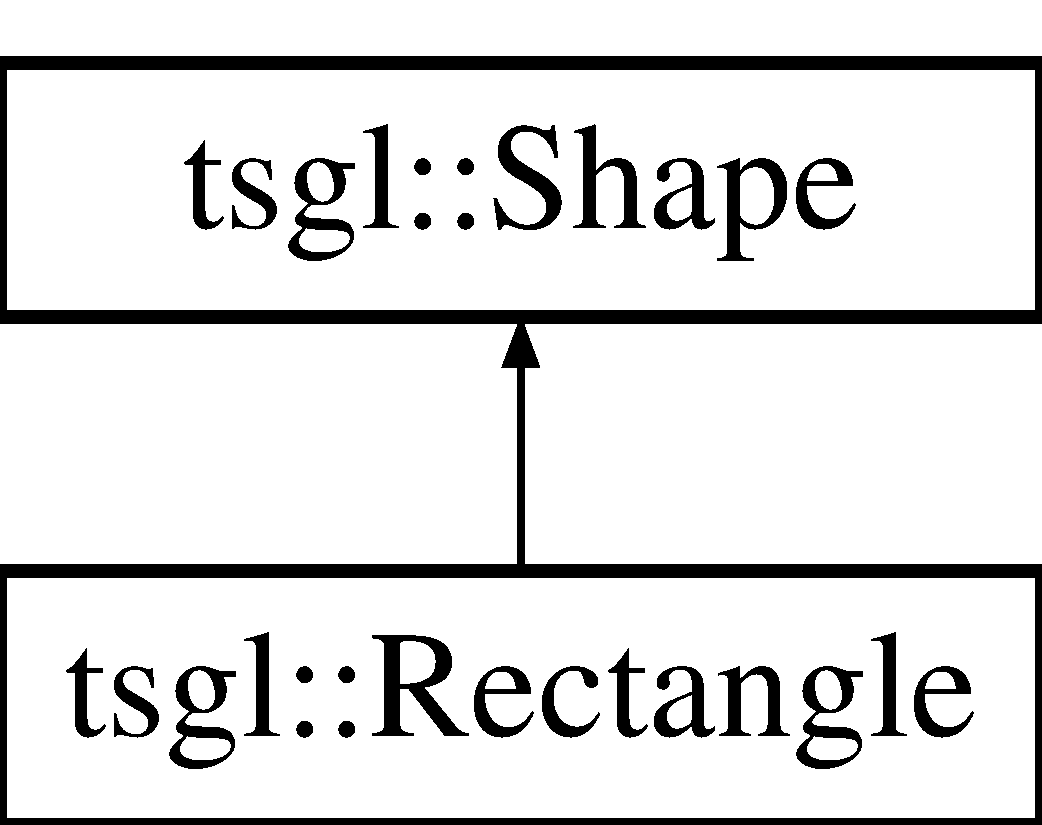
\includegraphics[height=2.000000cm]{classtsgl_1_1_rectangle}
\end{center}
\end{figure}
\subsection*{\-Public \-Member \-Functions}
\begin{DoxyCompactItemize}
\item 
\hyperlink{classtsgl_1_1_rectangle_a1fb2a492ffc57b2da380ea23d89e887b}{\-Rectangle} (int x, int y, int width, int height, const \hyperlink{structtsgl_1_1_color_float}{\-Color\-Float} \&color)
\begin{DoxyCompactList}\small\item\em \-Explicitly constructs a \hyperlink{classtsgl_1_1_rectangle}{\-Rectangle}. \end{DoxyCompactList}\item 
void \hyperlink{classtsgl_1_1_rectangle_addad1e65bc50d3669e6350aa32249c7f}{draw} ()
\begin{DoxyCompactList}\small\item\em \-Draw the \hyperlink{classtsgl_1_1_rectangle}{\-Rectangle}. \end{DoxyCompactList}\end{DoxyCompactItemize}


\subsection{\-Detailed \-Description}
\-Draw a simple \hyperlink{classtsgl_1_1_rectangle}{\-Rectangle}. 

\hyperlink{classtsgl_1_1_rectangle}{\-Rectangle} is a class for holding vertex data for a simple rectangle. 

\subsection{\-Constructor \& \-Destructor \-Documentation}
\hypertarget{classtsgl_1_1_rectangle_a1fb2a492ffc57b2da380ea23d89e887b}{\index{tsgl\-::\-Rectangle@{tsgl\-::\-Rectangle}!\-Rectangle@{\-Rectangle}}
\index{\-Rectangle@{\-Rectangle}!tsgl::Rectangle@{tsgl\-::\-Rectangle}}
\subsubsection[{\-Rectangle}]{\setlength{\rightskip}{0pt plus 5cm}{\bf tsgl\-::\-Rectangle\-::\-Rectangle} (
\begin{DoxyParamCaption}
\item[{int}]{x, }
\item[{int}]{y, }
\item[{int}]{width, }
\item[{int}]{height, }
\item[{const {\bf \-Color\-Float} \&}]{color}
\end{DoxyParamCaption}
)}}\label{classtsgl_1_1_rectangle_a1fb2a492ffc57b2da380ea23d89e887b}


\-Explicitly constructs a \hyperlink{classtsgl_1_1_rectangle}{\-Rectangle}. 

\-This is the constructor for the \hyperlink{classtsgl_1_1_rectangle}{\-Rectangle} class. 
\begin{DoxyParams}{\-Parameters}
{\em x} & \-The x coordinate of the \hyperlink{classtsgl_1_1_rectangle}{\-Rectangle}'s left edge. \\
\hline
{\em y} & \-The y coordinate of the \hyperlink{classtsgl_1_1_rectangle}{\-Rectangle}'s top edge. \\
\hline
{\em width} & \-The width of the \hyperlink{classtsgl_1_1_rectangle}{\-Rectangle}. \\
\hline
{\em height} & \-The height of the \hyperlink{classtsgl_1_1_rectangle}{\-Rectangle}. \\
\hline
{\em color} & \-The color of the \hyperlink{classtsgl_1_1_rectangle}{\-Rectangle}. \\
\hline
\end{DoxyParams}
\begin{DoxyReturn}{\-Returns}
\-A new \hyperlink{classtsgl_1_1_rectangle}{\-Rectangle} with the specified top left corner, dimensions, and color. 
\end{DoxyReturn}


\subsection{\-Member \-Function \-Documentation}
\hypertarget{classtsgl_1_1_rectangle_addad1e65bc50d3669e6350aa32249c7f}{\index{tsgl\-::\-Rectangle@{tsgl\-::\-Rectangle}!draw@{draw}}
\index{draw@{draw}!tsgl::Rectangle@{tsgl\-::\-Rectangle}}
\subsubsection[{draw}]{\setlength{\rightskip}{0pt plus 5cm}void {\bf tsgl\-::\-Rectangle\-::draw} (
\begin{DoxyParamCaption}
{}
\end{DoxyParamCaption}
)\hspace{0.3cm}{\ttfamily  \mbox{[}virtual\mbox{]}}}}\label{classtsgl_1_1_rectangle_addad1e65bc50d3669e6350aa32249c7f}


\-Draw the \hyperlink{classtsgl_1_1_rectangle}{\-Rectangle}. 

\-This function actually draws the \hyperlink{classtsgl_1_1_rectangle}{\-Rectangle} to the \hyperlink{classtsgl_1_1_canvas}{\-Canvas}. 

\-Implements \hyperlink{classtsgl_1_1_shape_af78b1627b97d621824ce86db214e2402}{tsgl\-::\-Shape}.



\-The documentation for this class was generated from the following files\-:\begin{DoxyCompactItemize}
\item 
\-Rectangle.\-h\item 
\-Rectangle.\-cpp\end{DoxyCompactItemize}

\hypertarget{classtsgl_1_1_round_function}{\section{tsgl\-:\-:\-Round\-Function \-Class \-Reference}
\label{classtsgl_1_1_round_function}\index{tsgl\-::\-Round\-Function@{tsgl\-::\-Round\-Function}}
}


\hyperlink{classtsgl_1_1_function}{\-Function} to round the input to the nearest integer number.  




{\ttfamily \#include $<$\-Function.\-h$>$}

\-Inheritance diagram for tsgl\-:\-:\-Round\-Function\-:\begin{figure}[H]
\begin{center}
\leavevmode
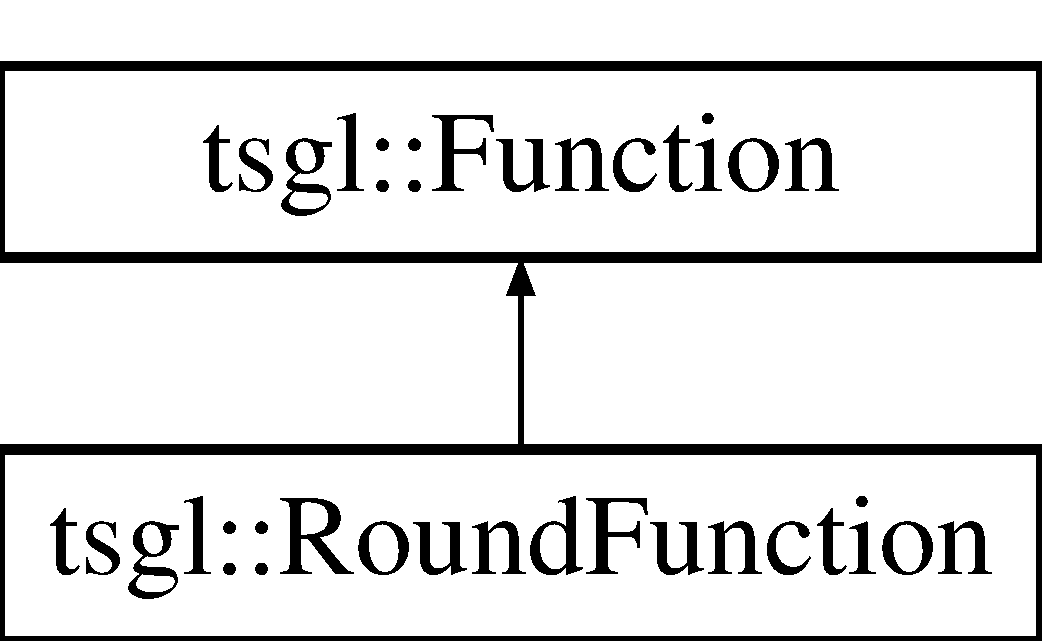
\includegraphics[height=2.000000cm]{classtsgl_1_1_round_function}
\end{center}
\end{figure}
\subsection*{\-Public \-Member \-Functions}
\begin{DoxyCompactItemize}
\item 
virtual \-Decimal \hyperlink{classtsgl_1_1_round_function_a3047ee723fae828d9379d946012028ca}{value\-At} (\-Decimal x) const 
\begin{DoxyCompactList}\small\item\em \-Method to determine the value of \hyperlink{classtsgl_1_1_round_function}{\-Round\-Function}. \end{DoxyCompactList}\end{DoxyCompactItemize}


\subsection{\-Detailed \-Description}
\hyperlink{classtsgl_1_1_function}{\-Function} to round the input to the nearest integer number. 

\subsection{\-Member \-Function \-Documentation}
\hypertarget{classtsgl_1_1_round_function_a3047ee723fae828d9379d946012028ca}{\index{tsgl\-::\-Round\-Function@{tsgl\-::\-Round\-Function}!value\-At@{value\-At}}
\index{value\-At@{value\-At}!tsgl::RoundFunction@{tsgl\-::\-Round\-Function}}
\subsubsection[{value\-At}]{\setlength{\rightskip}{0pt plus 5cm}virtual \-Decimal {\bf tsgl\-::\-Round\-Function\-::value\-At} (
\begin{DoxyParamCaption}
\item[{\-Decimal}]{x}
\end{DoxyParamCaption}
) const\hspace{0.3cm}{\ttfamily  \mbox{[}inline, virtual\mbox{]}}}}\label{classtsgl_1_1_round_function_a3047ee723fae828d9379d946012028ca}


\-Method to determine the value of \hyperlink{classtsgl_1_1_round_function}{\-Round\-Function}. 

\begin{DoxyReturn}{\-Returns}
\-The closest integer to $\ast$x$\ast$. 
\end{DoxyReturn}


\-Implements \hyperlink{classtsgl_1_1_function_affb7b3b19a04efefa29a9870d666e912}{tsgl\-::\-Function}.



\-The documentation for this class was generated from the following file\-:\begin{DoxyCompactItemize}
\item 
\-Function.\-h\end{DoxyCompactItemize}

\hypertarget{classtsgl_1_1_shape}{\section{tsgl\-:\-:Shape Class Reference}
\label{classtsgl_1_1_shape}\index{tsgl\-::\-Shape@{tsgl\-::\-Shape}}
}


A class for drawing shapes onto a \hyperlink{classtsgl_1_1_canvas}{Canvas} or \hyperlink{classtsgl_1_1_cartesian_canvas}{Cartesian\-Canvas}.  




{\ttfamily \#include $<$Shape.\-h$>$}

Inheritance diagram for tsgl\-:\-:Shape\-:\begin{figure}[H]
\begin{center}
\leavevmode
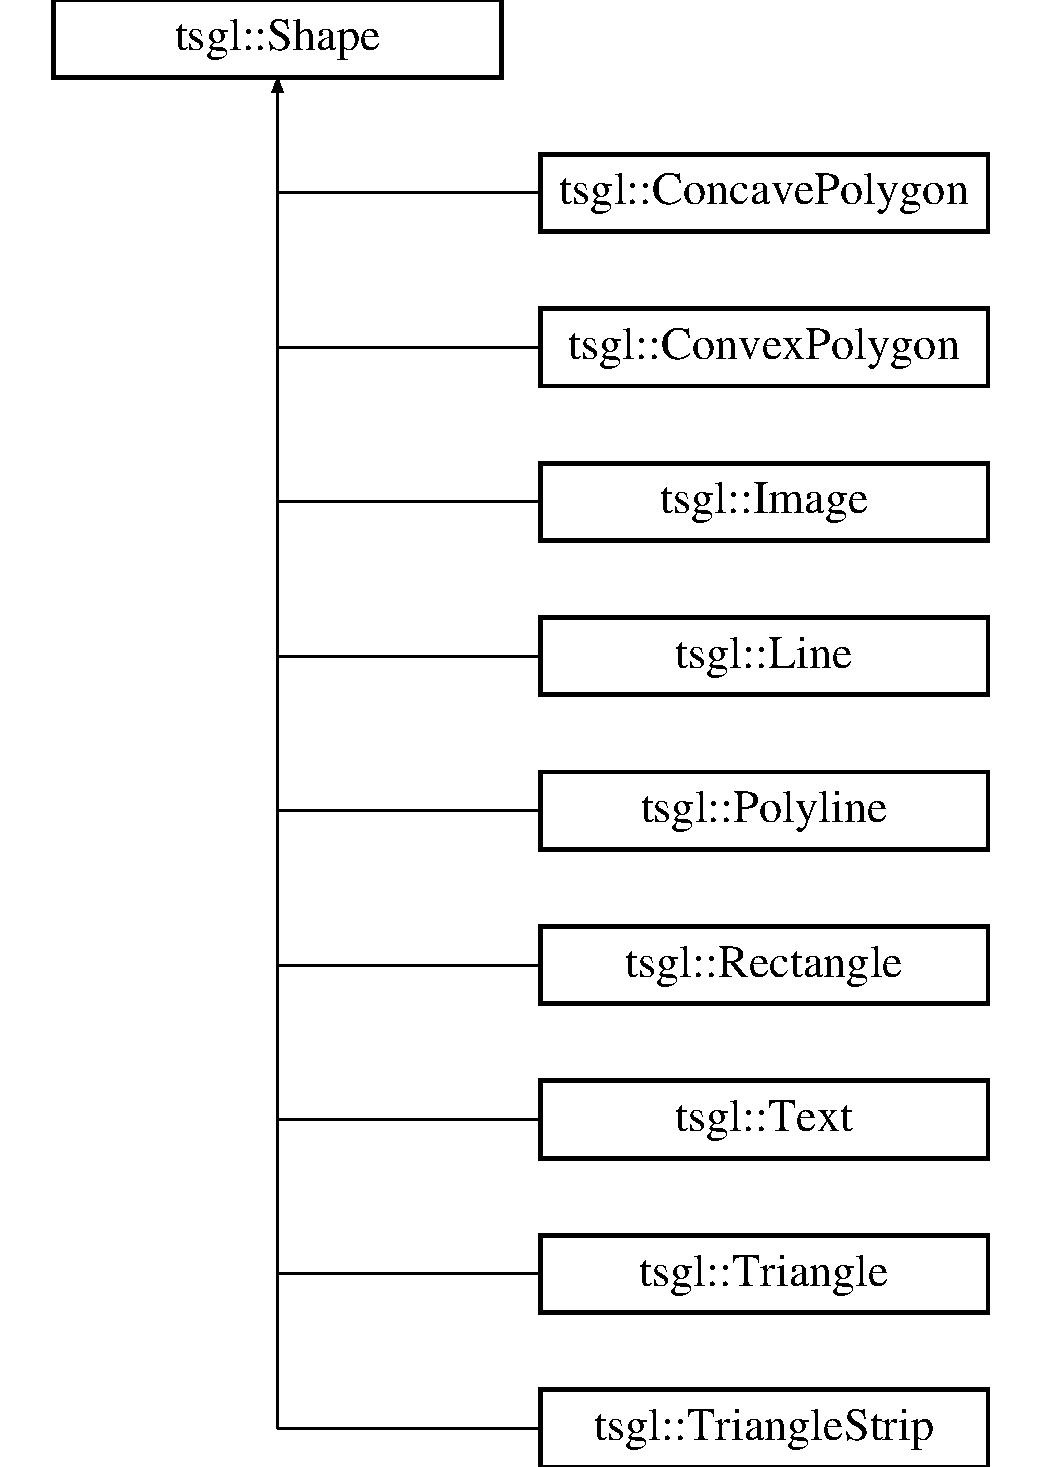
\includegraphics[height=10.000000cm]{classtsgl_1_1_shape}
\end{center}
\end{figure}
\subsection*{Public Member Functions}
\begin{DoxyCompactItemize}
\item 
\hyperlink{classtsgl_1_1_shape_ad283a47aa40bf80dcd308cc581c9e2dd}{Shape} ()
\begin{DoxyCompactList}\small\item\em Constructs a new \hyperlink{classtsgl_1_1_shape}{Shape}. \end{DoxyCompactList}\item 
\hypertarget{classtsgl_1_1_shape_aa9bfac883a0748471600fe9752e85948}{virtual \hyperlink{classtsgl_1_1_shape_aa9bfac883a0748471600fe9752e85948}{$\sim$\-Shape} ()}\label{classtsgl_1_1_shape_aa9bfac883a0748471600fe9752e85948}

\begin{DoxyCompactList}\small\item\em Destructor for the \hyperlink{classtsgl_1_1_shape}{Shape}. \end{DoxyCompactList}\item 
virtual void \hyperlink{classtsgl_1_1_shape_af78b1627b97d621824ce86db214e2402}{draw} ()=0
\begin{DoxyCompactList}\small\item\em Actually draws the \hyperlink{classtsgl_1_1_shape}{Shape} to the \hyperlink{classtsgl_1_1_canvas}{Canvas}. \end{DoxyCompactList}\item 
bool \hyperlink{classtsgl_1_1_shape_aadd0ea81f714328bdf9483851a8b86ad}{get\-Is\-Textured} ()
\begin{DoxyCompactList}\small\item\em Accessor for {\ttfamily is\-Textured}. \end{DoxyCompactList}\end{DoxyCompactItemize}
\subsection*{Protected Attributes}
\begin{DoxyCompactItemize}
\item 
\hypertarget{classtsgl_1_1_shape_a9d5cd6d6a0596a30dbce44eb2d00c583}{bool {\bfseries is\-Textured}}\label{classtsgl_1_1_shape_a9d5cd6d6a0596a30dbce44eb2d00c583}

\end{DoxyCompactItemize}


\subsection{Detailed Description}
A class for drawing shapes onto a \hyperlink{classtsgl_1_1_canvas}{Canvas} or \hyperlink{classtsgl_1_1_cartesian_canvas}{Cartesian\-Canvas}. 

\begin{DoxyWarning}{Warning}
{\bfseries {\itshape Though extending this class must be allowed due to the way the code is set up, attempting to do so could potentially mess up the internal G\-L calls the library uses. Proceed with great caution.}}
\end{DoxyWarning}
\hyperlink{classtsgl_1_1_shape}{Shape} provides a base class for drawing shapes to a \hyperlink{classtsgl_1_1_canvas}{Canvas} or \hyperlink{classtsgl_1_1_cartesian_canvas}{Cartesian\-Canvas}. \begin{DoxyNote}{Note}
\hyperlink{classtsgl_1_1_shape}{Shape} is abstract, and must be extended by the user.
\end{DoxyNote}
All \hyperlink{classtsgl_1_1_shape}{Shape} subclasses must override the \hyperlink{classtsgl_1_1_shape_af78b1627b97d621824ce86db214e2402}{draw()} method. Though theoretically any G\-L calls can be used here, something like the following should be used\-: {\ttfamily  gl\-Buffer\-Data(\-G\-L\-\_\-\-A\-R\-R\-A\-Y\-\_\-\-B\-U\-F\-F\-E\-R, numberofvertices $\ast$ 6 $\ast$ sizeof(float), vertices, G\-L\-\_\-\-D\-Y\-N\-A\-M\-I\-C\-\_\-\-D\-R\-A\-W); gl\-Draw\-Arrays(drawingmode, 0, numberofvertices); }

{\ttfamily vertices} should be an array of floating point values in T\-S\-G\-L's vertex format. One vertex consists of 6 floating point values, signifying x,y,red,green,blue,and alpha components respectively. E.\-g., to draw a triangle, you would need 3 vertices = 18 floats -\/$>$ vertices should be an array of length 18.

{\ttfamily numberofvertices} should be the actual integer number of vertices to be drawn (e.\-g., {\itshape 3} for a triangle).

{\ttfamily drawingmode} should be one of G\-L's primitive drawing modes. See \href{https://www.opengl.org/sdk/docs/man2/xhtml/glBegin.xml}{\tt https\-://www.\-opengl.\-org/sdk/docs/man2/xhtml/gl\-Begin.\-xml} for further information.

Theoretically, you could potentially extend the \hyperlink{classtsgl_1_1_shape}{Shape} class so that you can create another \hyperlink{classtsgl_1_1_shape}{Shape} class that suits your needs.

However, this is not recommended for normal use of the T\-S\-G\-L library. 

\subsection{Constructor \& Destructor Documentation}
\hypertarget{classtsgl_1_1_shape_ad283a47aa40bf80dcd308cc581c9e2dd}{\index{tsgl\-::\-Shape@{tsgl\-::\-Shape}!Shape@{Shape}}
\index{Shape@{Shape}!tsgl::Shape@{tsgl\-::\-Shape}}
\subsubsection[{Shape}]{\setlength{\rightskip}{0pt plus 5cm}tsgl\-::\-Shape\-::\-Shape (
\begin{DoxyParamCaption}
{}
\end{DoxyParamCaption}
)\hspace{0.3cm}{\ttfamily [inline]}}}\label{classtsgl_1_1_shape_ad283a47aa40bf80dcd308cc581c9e2dd}


Constructs a new \hyperlink{classtsgl_1_1_shape}{Shape}. 

Whether the shape is textured or not. If extending \hyperlink{classtsgl_1_1_shape}{Shape}, {\bfseries  you {\itshape must} leave this at false (unless you are working with an image). }


\begin{DoxyItemize}
\item Usually {\ttfamily vertices} is filled with floating point values that represent the vertices of the shape to be drawn.
\item You may define other items in the constructor that pertain to the attributes of the subclass that is extending \hyperlink{classtsgl_1_1_shape}{Shape}.
\item At a minimum, you {\itshape M\-U\-S\-T} fill an array of floating point values that pertain to the vertices of the shape. \begin{DoxyWarning}{Warning}
{\bfseries You {\itshape must} inherit the parent's constructor if you are extending \hyperlink{classtsgl_1_1_shape}{Shape}.} 
\end{DoxyWarning}
\begin{DoxyNote}{Note}
Refer to the \hyperlink{classtsgl_1_1_shape}{Shape} class description for more details. 
\end{DoxyNote}

\end{DoxyItemize}

\subsection{Member Function Documentation}
\hypertarget{classtsgl_1_1_shape_af78b1627b97d621824ce86db214e2402}{\index{tsgl\-::\-Shape@{tsgl\-::\-Shape}!draw@{draw}}
\index{draw@{draw}!tsgl::Shape@{tsgl\-::\-Shape}}
\subsubsection[{draw}]{\setlength{\rightskip}{0pt plus 5cm}virtual void tsgl\-::\-Shape\-::draw (
\begin{DoxyParamCaption}
{}
\end{DoxyParamCaption}
)\hspace{0.3cm}{\ttfamily [pure virtual]}}}\label{classtsgl_1_1_shape_af78b1627b97d621824ce86db214e2402}


Actually draws the \hyperlink{classtsgl_1_1_shape}{Shape} to the \hyperlink{classtsgl_1_1_canvas}{Canvas}. 

This method renders the shape to the \hyperlink{classtsgl_1_1_canvas}{Canvas}.
\begin{DoxyItemize}
\item When you extend the \hyperlink{classtsgl_1_1_shape}{Shape} class, you {\itshape M\-U\-S\-T} provide a definition for this method.
\item The definition must follow this format\-: {\ttfamily  gl\-Buffer\-Data(drawing\-Mode, number\-Of\-Vertices $\ast$ 6 $\ast$ sizeof(float), vertices, G\-L\-\_\-\-D\-Y\-N\-A\-M\-I\-C\-\_\-\-D\-R\-A\-W); gl\-Draw\-Arrays(drawing\-Mode, 0, number\-Of\-Vertices); }
\item Really bad things could potentially happen if you do not follow this format. These two statements {\itshape M\-U\-S\-T} be in the \hyperlink{classtsgl_1_1_shape_af78b1627b97d621824ce86db214e2402}{draw()} method of the subclass that extends the \hyperlink{classtsgl_1_1_shape}{Shape} class.
\item You can add other statements in the subclass \begin{DoxyNote}{Note}
Please refer to the class description for more information and warnings about overriding this method. 
\end{DoxyNote}

\end{DoxyItemize}

Implemented in \hyperlink{classtsgl_1_1_concave_polygon_a06d759932483ae2b54bb807db20cbc4a}{tsgl\-::\-Concave\-Polygon}, \hyperlink{classtsgl_1_1_convex_polygon_add4d4971a5d22385eebbfe771af916b5}{tsgl\-::\-Convex\-Polygon}, \hyperlink{classtsgl_1_1_triangle_strip_a7a984063f85c8b6ab61bd6e989d38920}{tsgl\-::\-Triangle\-Strip}, \hyperlink{classtsgl_1_1_polyline_ac6de5e2817824d9427d02d3e7be37f47}{tsgl\-::\-Polyline}, \hyperlink{classtsgl_1_1_image_a85732de312b98dd5ce5a9cc319bbf8c5}{tsgl\-::\-Image}, \hyperlink{classtsgl_1_1_text_a9dc47e4af682abfdab74e37b71f9fbde}{tsgl\-::\-Text}, \hyperlink{classtsgl_1_1_triangle_a83b30f9f7c800146fa900d32a58fa0c7}{tsgl\-::\-Triangle}, \hyperlink{classtsgl_1_1_line_ae7eccbbf5230a4c68139560d810af415}{tsgl\-::\-Line}, and \hyperlink{classtsgl_1_1_rectangle_addad1e65bc50d3669e6350aa32249c7f}{tsgl\-::\-Rectangle}.

\hypertarget{classtsgl_1_1_shape_aadd0ea81f714328bdf9483851a8b86ad}{\index{tsgl\-::\-Shape@{tsgl\-::\-Shape}!get\-Is\-Textured@{get\-Is\-Textured}}
\index{get\-Is\-Textured@{get\-Is\-Textured}!tsgl::Shape@{tsgl\-::\-Shape}}
\subsubsection[{get\-Is\-Textured}]{\setlength{\rightskip}{0pt plus 5cm}bool tsgl\-::\-Shape\-::get\-Is\-Textured (
\begin{DoxyParamCaption}
{}
\end{DoxyParamCaption}
)\hspace{0.3cm}{\ttfamily [inline]}}}\label{classtsgl_1_1_shape_aadd0ea81f714328bdf9483851a8b86ad}


Accessor for {\ttfamily is\-Textured}. 

\begin{DoxyReturn}{Returns}
Whether the shape is a textured primitive or not. 
\end{DoxyReturn}


The documentation for this class was generated from the following file\-:\begin{DoxyCompactItemize}
\item 
Shape.\-h\end{DoxyCompactItemize}

\hypertarget{classtsgl_1_1_sine_function}{}\section{tsgl\+:\+:Sine\+Function Class Reference}
\label{classtsgl_1_1_sine_function}\index{tsgl\+::\+Sine\+Function@{tsgl\+::\+Sine\+Function}}


\hyperlink{classtsgl_1_1_function}{Function} to compute the sine of the input.  




{\ttfamily \#include $<$Function.\+h$>$}

Inheritance diagram for tsgl\+:\+:Sine\+Function\+:\begin{figure}[H]
\begin{center}
\leavevmode
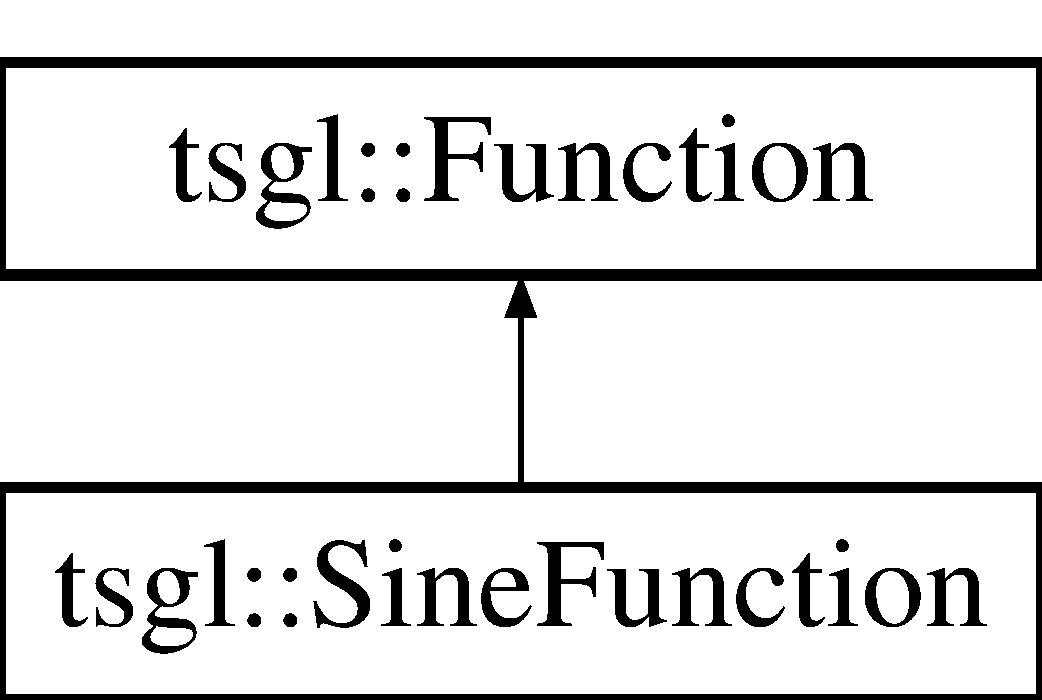
\includegraphics[height=2.000000cm]{classtsgl_1_1_sine_function}
\end{center}
\end{figure}
\subsection*{Public Member Functions}
\begin{DoxyCompactItemize}
\item 
virtual Decimal \hyperlink{classtsgl_1_1_sine_function_a6507b049141d946ede1611050e44dab2}{value\+At} (Decimal x) const 
\begin{DoxyCompactList}\small\item\em Method to determine the value of \hyperlink{classtsgl_1_1_sine_function}{Sine\+Function}. \end{DoxyCompactList}\end{DoxyCompactItemize}


\subsection{Detailed Description}
\hyperlink{classtsgl_1_1_function}{Function} to compute the sine of the input. 

\subsection{Member Function Documentation}
\hypertarget{classtsgl_1_1_sine_function_a6507b049141d946ede1611050e44dab2}{}\index{tsgl\+::\+Sine\+Function@{tsgl\+::\+Sine\+Function}!value\+At@{value\+At}}
\index{value\+At@{value\+At}!tsgl\+::\+Sine\+Function@{tsgl\+::\+Sine\+Function}}
\subsubsection[{value\+At}]{\setlength{\rightskip}{0pt plus 5cm}virtual Decimal tsgl\+::\+Sine\+Function\+::value\+At (
\begin{DoxyParamCaption}
\item[{Decimal}]{x}
\end{DoxyParamCaption}
) const\hspace{0.3cm}{\ttfamily [inline]}, {\ttfamily [virtual]}}\label{classtsgl_1_1_sine_function_a6507b049141d946ede1611050e44dab2}


Method to determine the value of \hyperlink{classtsgl_1_1_sine_function}{Sine\+Function}. 

\begin{DoxyReturn}{Returns}
The sine of {\itshape x}. 
\end{DoxyReturn}


Implements \hyperlink{classtsgl_1_1_function_affb7b3b19a04efefa29a9870d666e912}{tsgl\+::\+Function}.



The documentation for this class was generated from the following file\+:\begin{DoxyCompactItemize}
\item 
Function.\+h\end{DoxyCompactItemize}

\hypertarget{classtsgl_1_1_spectrogram}{\section{tsgl\-:\-:\-Spectrogram \-Class \-Reference}
\label{classtsgl_1_1_spectrogram}\index{tsgl\-::\-Spectrogram@{tsgl\-::\-Spectrogram}}
}


\-Displays a spectrogram of a given data set.  




{\ttfamily \#include $<$\-Spectrogram.\-h$>$}

\subsection*{\-Public \-Member \-Functions}
\begin{DoxyCompactItemize}
\item 
\hyperlink{classtsgl_1_1_spectrogram_a806d3244b086b9ed2c982b7178eb5139}{\-Spectrogram} (\-Spectrogram\-Drawmode draw\-Mode, int width, int height=-\/1)
\begin{DoxyCompactList}\small\item\em \-Explicit \hyperlink{classtsgl_1_1_spectrogram}{\-Spectrogram} constructor method. \end{DoxyCompactList}\item 
\hyperlink{classtsgl_1_1_spectrogram_abf1ff8d5acade39017321d6a2006f0f1}{$\sim$\-Spectrogram} ()
\begin{DoxyCompactList}\small\item\em \hyperlink{classtsgl_1_1_spectrogram}{\-Spectrogram} destructor method. \end{DoxyCompactList}\item 
void \hyperlink{classtsgl_1_1_spectrogram_a52be3a5f280c4fe6b82960283df7d91d}{update\-Locked} (int index, float weight=1.\-0f, float decay=0.\-8f)
\begin{DoxyCompactList}\small\item\em \-Updates a spectrogram with new data, using locks for thread safety. \end{DoxyCompactList}\item 
void \hyperlink{classtsgl_1_1_spectrogram_a671efc29173bc9c5578090c3d4ff331a}{update\-Critical} (int index, float weight=1.\-0f, float decay=0.\-8f)
\begin{DoxyCompactList}\small\item\em \-Updates a spectrogram with new data, using critical sections for thread safety. \end{DoxyCompactList}\item 
void \hyperlink{classtsgl_1_1_spectrogram_aef15257f0daa13a57d99cd621d402bd5}{draw} (float ratio)
\begin{DoxyCompactList}\small\item\em \-Updates the image on the spectrogram. \end{DoxyCompactList}\item 
void \hyperlink{classtsgl_1_1_spectrogram_a9e6eb0489ee0fb9f96b2a5202868a1c2}{finish} ()
\begin{DoxyCompactList}\small\item\em \-Finishes the spectrogram. \end{DoxyCompactList}\end{DoxyCompactItemize}


\subsection{\-Detailed \-Description}
\-Displays a spectrogram of a given data set. 

\hyperlink{classtsgl_1_1_spectrogram}{\-Spectrogram} is a class for visualizing data as a color spectrum. \-This data will typically be hues, but \hyperlink{classtsgl_1_1_spectrogram}{\-Spectrogram} will accept any data mapping to an integer value between 0 and 255. 

\subsection{\-Constructor \& \-Destructor \-Documentation}
\hypertarget{classtsgl_1_1_spectrogram_a806d3244b086b9ed2c982b7178eb5139}{\index{tsgl\-::\-Spectrogram@{tsgl\-::\-Spectrogram}!\-Spectrogram@{\-Spectrogram}}
\index{\-Spectrogram@{\-Spectrogram}!tsgl::Spectrogram@{tsgl\-::\-Spectrogram}}
\subsubsection[{\-Spectrogram}]{\setlength{\rightskip}{0pt plus 5cm}{\bf tsgl\-::\-Spectrogram\-::\-Spectrogram} (
\begin{DoxyParamCaption}
\item[{\-Spectrogram\-Drawmode}]{draw\-Mode, }
\item[{int}]{width, }
\item[{int}]{height = {\ttfamily -\/1}}
\end{DoxyParamCaption}
)}}\label{classtsgl_1_1_spectrogram_a806d3244b086b9ed2c982b7178eb5139}


\-Explicit \hyperlink{classtsgl_1_1_spectrogram}{\-Spectrogram} constructor method. 

\-This is the explicit constructor for the \hyperlink{classtsgl_1_1_spectrogram}{\-Spectrogram} class. 
\begin{DoxyParams}{\-Parameters}
{\em draw\-Mode} & \-Method used for displaying spectral data. \-Can be one of \-C\-I\-R\-C\-U\-L\-A\-R or \-H\-O\-R\-I\-Z\-O\-N\-T\-A\-L. \\
\hline
{\em width} & \-The width of the \hyperlink{classtsgl_1_1_spectrogram}{\-Spectrogram} canvas. \\
\hline
{\em height} & \-The height of the \hyperlink{classtsgl_1_1_spectrogram}{\-Spectrogram} canvas. \-This value is ignored for \-H\-O\-R\-I\-Z\-O\-N\-T\-A\-L \-Spectrograms. \-Setting this to -\/1 sets the width automatically. \\
\hline
\end{DoxyParams}
\begin{DoxyReturn}{\-Returns}
\-A new \hyperlink{classtsgl_1_1_spectrogram}{\-Spectrogram} with the specified drawing mode and size. 
\end{DoxyReturn}
\hypertarget{classtsgl_1_1_spectrogram_abf1ff8d5acade39017321d6a2006f0f1}{\index{tsgl\-::\-Spectrogram@{tsgl\-::\-Spectrogram}!$\sim$\-Spectrogram@{$\sim$\-Spectrogram}}
\index{$\sim$\-Spectrogram@{$\sim$\-Spectrogram}!tsgl::Spectrogram@{tsgl\-::\-Spectrogram}}
\subsubsection[{$\sim$\-Spectrogram}]{\setlength{\rightskip}{0pt plus 5cm}{\bf tsgl\-::\-Spectrogram\-::$\sim$\-Spectrogram} (
\begin{DoxyParamCaption}
{}
\end{DoxyParamCaption}
)}}\label{classtsgl_1_1_spectrogram_abf1ff8d5acade39017321d6a2006f0f1}


\hyperlink{classtsgl_1_1_spectrogram}{\-Spectrogram} destructor method. 

\-This is the destructor for the \hyperlink{classtsgl_1_1_spectrogram}{\-Spectrogram} class.

\-Frees up memory that was allocated to a \hyperlink{classtsgl_1_1_spectrogram}{\-Spectrogram} instance. 

\subsection{\-Member \-Function \-Documentation}
\hypertarget{classtsgl_1_1_spectrogram_aef15257f0daa13a57d99cd621d402bd5}{\index{tsgl\-::\-Spectrogram@{tsgl\-::\-Spectrogram}!draw@{draw}}
\index{draw@{draw}!tsgl::Spectrogram@{tsgl\-::\-Spectrogram}}
\subsubsection[{draw}]{\setlength{\rightskip}{0pt plus 5cm}void {\bf tsgl\-::\-Spectrogram\-::draw} (
\begin{DoxyParamCaption}
\item[{float}]{ratio}
\end{DoxyParamCaption}
)}}\label{classtsgl_1_1_spectrogram_aef15257f0daa13a57d99cd621d402bd5}


\-Updates the image on the spectrogram. 

\-This function updates the \hyperlink{classtsgl_1_1_spectrogram}{\-Spectrogram}'s \hyperlink{classtsgl_1_1_canvas}{\-Canvas} with the data since the last call to update() and redraws it. 
\begin{DoxyParams}{\-Parameters}
{\em ratio} & \-The scaling of the visualizer. \-Accepts values between 0.\-0f and 1.\-0f. \\
\hline
\end{DoxyParams}
\hypertarget{classtsgl_1_1_spectrogram_a9e6eb0489ee0fb9f96b2a5202868a1c2}{\index{tsgl\-::\-Spectrogram@{tsgl\-::\-Spectrogram}!finish@{finish}}
\index{finish@{finish}!tsgl::Spectrogram@{tsgl\-::\-Spectrogram}}
\subsubsection[{finish}]{\setlength{\rightskip}{0pt plus 5cm}void {\bf tsgl\-::\-Spectrogram\-::finish} (
\begin{DoxyParamCaption}
{}
\end{DoxyParamCaption}
)}}\label{classtsgl_1_1_spectrogram_a9e6eb0489ee0fb9f96b2a5202868a1c2}


\-Finishes the spectrogram. 

\-This function tells the \hyperlink{classtsgl_1_1_spectrogram}{\-Spectrogram} to free all of its memory and close down its \hyperlink{classtsgl_1_1_canvas}{\-Canvas}. \hypertarget{classtsgl_1_1_spectrogram_a671efc29173bc9c5578090c3d4ff331a}{\index{tsgl\-::\-Spectrogram@{tsgl\-::\-Spectrogram}!update\-Critical@{update\-Critical}}
\index{update\-Critical@{update\-Critical}!tsgl::Spectrogram@{tsgl\-::\-Spectrogram}}
\subsubsection[{update\-Critical}]{\setlength{\rightskip}{0pt plus 5cm}void {\bf tsgl\-::\-Spectrogram\-::update\-Critical} (
\begin{DoxyParamCaption}
\item[{int}]{index, }
\item[{float}]{weight = {\ttfamily 1.0f}, }
\item[{float}]{decay = {\ttfamily 0.8f}}
\end{DoxyParamCaption}
)}}\label{classtsgl_1_1_spectrogram_a671efc29173bc9c5578090c3d4ff331a}


\-Updates a spectrogram with new data, using critical sections for thread safety. 

\-This function adds the value of {\ttfamily weight} to the hue specified by {\ttfamily index}, and adds the value ({\ttfamily decay}$^\wedge${\ttfamily n})$\ast$ {\ttfamily weight} to all hues {\ttfamily n} steps away from {\ttfamily index}. 
\begin{DoxyParams}{\-Parameters}
{\em index} & \-Index of the hue to update. \-Value is taken mod 256. \\
\hline
{\em weight} & \-The value to add to {\ttfamily index}. \\
\hline
{\em decay} & \-Falloff for {\ttfamily weight} upon adjacent values. \\
\hline
\end{DoxyParams}
\hypertarget{classtsgl_1_1_spectrogram_a52be3a5f280c4fe6b82960283df7d91d}{\index{tsgl\-::\-Spectrogram@{tsgl\-::\-Spectrogram}!update\-Locked@{update\-Locked}}
\index{update\-Locked@{update\-Locked}!tsgl::Spectrogram@{tsgl\-::\-Spectrogram}}
\subsubsection[{update\-Locked}]{\setlength{\rightskip}{0pt plus 5cm}void {\bf tsgl\-::\-Spectrogram\-::update\-Locked} (
\begin{DoxyParamCaption}
\item[{int}]{index, }
\item[{float}]{weight = {\ttfamily 1.0f}, }
\item[{float}]{decay = {\ttfamily 0.8f}}
\end{DoxyParamCaption}
)}}\label{classtsgl_1_1_spectrogram_a52be3a5f280c4fe6b82960283df7d91d}


\-Updates a spectrogram with new data, using locks for thread safety. 

\-This function adds the value of {\ttfamily weight} to the hue specified by {\ttfamily index}, and adds the value ({\ttfamily decay}$^\wedge${\ttfamily n})$\ast$ {\ttfamily weight} to all hues {\ttfamily n} steps away from {\ttfamily index}. 
\begin{DoxyParams}{\-Parameters}
{\em index} & \-Index of the hue to update. \-Value is taken mod 256. \\
\hline
{\em weight} & \-The value to add to {\ttfamily index}. \\
\hline
{\em decay} & \-Falloff for {\ttfamily weight} upon adjacent values. \\
\hline
\end{DoxyParams}


\-The documentation for this class was generated from the following files\-:\begin{DoxyCompactItemize}
\item 
\-Spectrogram.\-h\item 
\-Spectrogram.\-cpp\end{DoxyCompactItemize}

\hypertarget{classtsgl_1_1_square_root_function}{\section{tsgl\-:\-:Square\-Root\-Function Class Reference}
\label{classtsgl_1_1_square_root_function}\index{tsgl\-::\-Square\-Root\-Function@{tsgl\-::\-Square\-Root\-Function}}
}


\hyperlink{classtsgl_1_1_function}{Function} to compute the square root of the input.  




{\ttfamily \#include $<$Function.\-h$>$}

Inheritance diagram for tsgl\-:\-:Square\-Root\-Function\-:\begin{figure}[H]
\begin{center}
\leavevmode
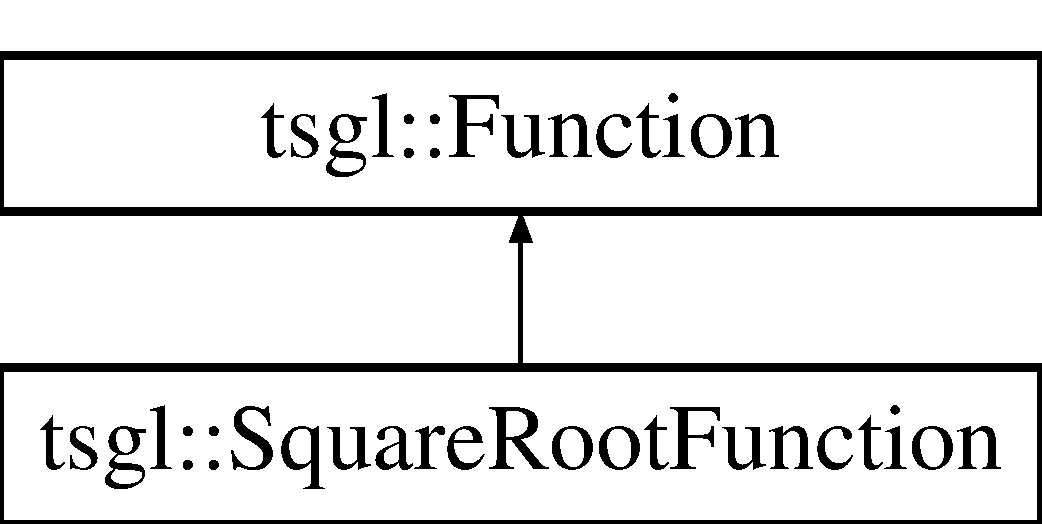
\includegraphics[height=2.000000cm]{classtsgl_1_1_square_root_function}
\end{center}
\end{figure}
\subsection*{Public Member Functions}
\begin{DoxyCompactItemize}
\item 
virtual Decimal \hyperlink{classtsgl_1_1_square_root_function_a25f6192ef7b12b80c4a14186e1cde97c}{value\-At} (Decimal x) const 
\begin{DoxyCompactList}\small\item\em Method to determine the value of \hyperlink{classtsgl_1_1_square_root_function}{Square\-Root\-Function}. \end{DoxyCompactList}\end{DoxyCompactItemize}


\subsection{Detailed Description}
\hyperlink{classtsgl_1_1_function}{Function} to compute the square root of the input. 

\subsection{Member Function Documentation}
\hypertarget{classtsgl_1_1_square_root_function_a25f6192ef7b12b80c4a14186e1cde97c}{\index{tsgl\-::\-Square\-Root\-Function@{tsgl\-::\-Square\-Root\-Function}!value\-At@{value\-At}}
\index{value\-At@{value\-At}!tsgl::SquareRootFunction@{tsgl\-::\-Square\-Root\-Function}}
\subsubsection[{value\-At}]{\setlength{\rightskip}{0pt plus 5cm}virtual Decimal tsgl\-::\-Square\-Root\-Function\-::value\-At (
\begin{DoxyParamCaption}
\item[{Decimal}]{x}
\end{DoxyParamCaption}
) const\hspace{0.3cm}{\ttfamily [inline]}, {\ttfamily [virtual]}}}\label{classtsgl_1_1_square_root_function_a25f6192ef7b12b80c4a14186e1cde97c}


Method to determine the value of \hyperlink{classtsgl_1_1_square_root_function}{Square\-Root\-Function}. 

\begin{DoxyReturn}{Returns}
The square root of {\itshape x}. 
\end{DoxyReturn}


Implements \hyperlink{classtsgl_1_1_function_affb7b3b19a04efefa29a9870d666e912}{tsgl\-::\-Function}.



The documentation for this class was generated from the following file\-:\begin{DoxyCompactItemize}
\item 
Function.\-h\end{DoxyCompactItemize}

\hypertarget{classtsgl_1_1_tangent_function}{\section{tsgl\-:\-:Tangent\-Function Class Reference}
\label{classtsgl_1_1_tangent_function}\index{tsgl\-::\-Tangent\-Function@{tsgl\-::\-Tangent\-Function}}
}


\hyperlink{classtsgl_1_1_function}{Function} to compute the tangent of the input.  




{\ttfamily \#include $<$Function.\-h$>$}

Inheritance diagram for tsgl\-:\-:Tangent\-Function\-:\begin{figure}[H]
\begin{center}
\leavevmode
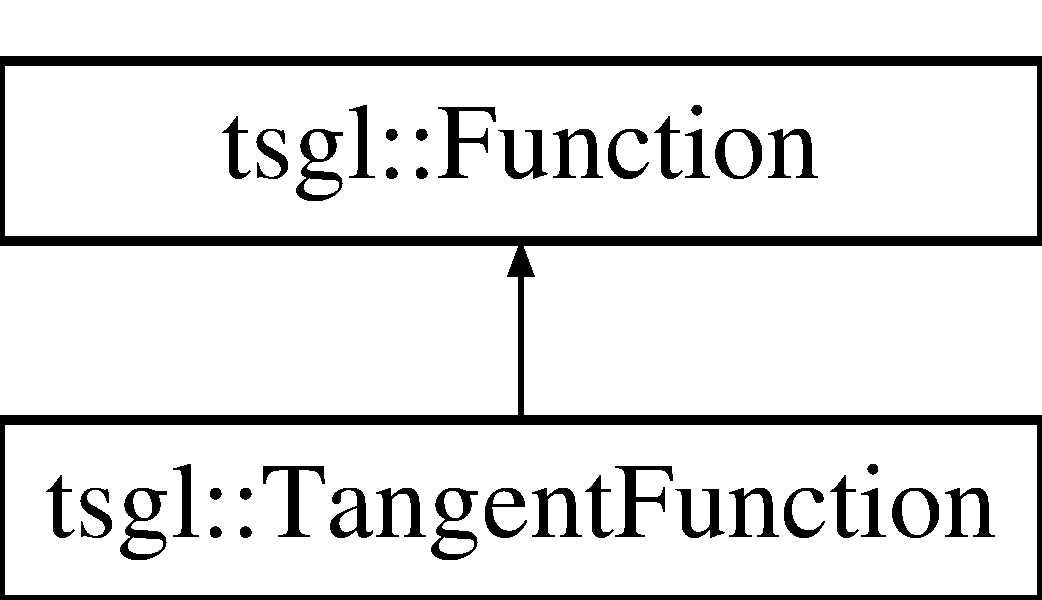
\includegraphics[height=2.000000cm]{classtsgl_1_1_tangent_function}
\end{center}
\end{figure}
\subsection*{Public Member Functions}
\begin{DoxyCompactItemize}
\item 
virtual Decimal \hyperlink{classtsgl_1_1_tangent_function_a3737542399069ebce368a5b53ba8a563}{value\-At} (Decimal x) const 
\begin{DoxyCompactList}\small\item\em Method to determine the value of \hyperlink{classtsgl_1_1_tangent_function}{Tangent\-Function}. \end{DoxyCompactList}\end{DoxyCompactItemize}


\subsection{Detailed Description}
\hyperlink{classtsgl_1_1_function}{Function} to compute the tangent of the input. 

\subsection{Member Function Documentation}
\hypertarget{classtsgl_1_1_tangent_function_a3737542399069ebce368a5b53ba8a563}{\index{tsgl\-::\-Tangent\-Function@{tsgl\-::\-Tangent\-Function}!value\-At@{value\-At}}
\index{value\-At@{value\-At}!tsgl::TangentFunction@{tsgl\-::\-Tangent\-Function}}
\subsubsection[{value\-At}]{\setlength{\rightskip}{0pt plus 5cm}virtual Decimal tsgl\-::\-Tangent\-Function\-::value\-At (
\begin{DoxyParamCaption}
\item[{Decimal}]{x}
\end{DoxyParamCaption}
) const\hspace{0.3cm}{\ttfamily [inline]}, {\ttfamily [virtual]}}}\label{classtsgl_1_1_tangent_function_a3737542399069ebce368a5b53ba8a563}


Method to determine the value of \hyperlink{classtsgl_1_1_tangent_function}{Tangent\-Function}. 

\begin{DoxyReturn}{Returns}
The tangent of {\itshape x}. 
\end{DoxyReturn}


Implements \hyperlink{classtsgl_1_1_function_affb7b3b19a04efefa29a9870d666e912}{tsgl\-::\-Function}.



The documentation for this class was generated from the following file\-:\begin{DoxyCompactItemize}
\item 
Function.\-h\end{DoxyCompactItemize}

\hypertarget{classtsgl_1_1_text}{\section{tsgl\-:\-:\-Text \-Class \-Reference}
\label{classtsgl_1_1_text}\index{tsgl\-::\-Text@{tsgl\-::\-Text}}
}


\-Draw a string of text.  




{\ttfamily \#include $<$\-Text.\-h$>$}

\-Inheritance diagram for tsgl\-:\-:\-Text\-:\begin{figure}[H]
\begin{center}
\leavevmode
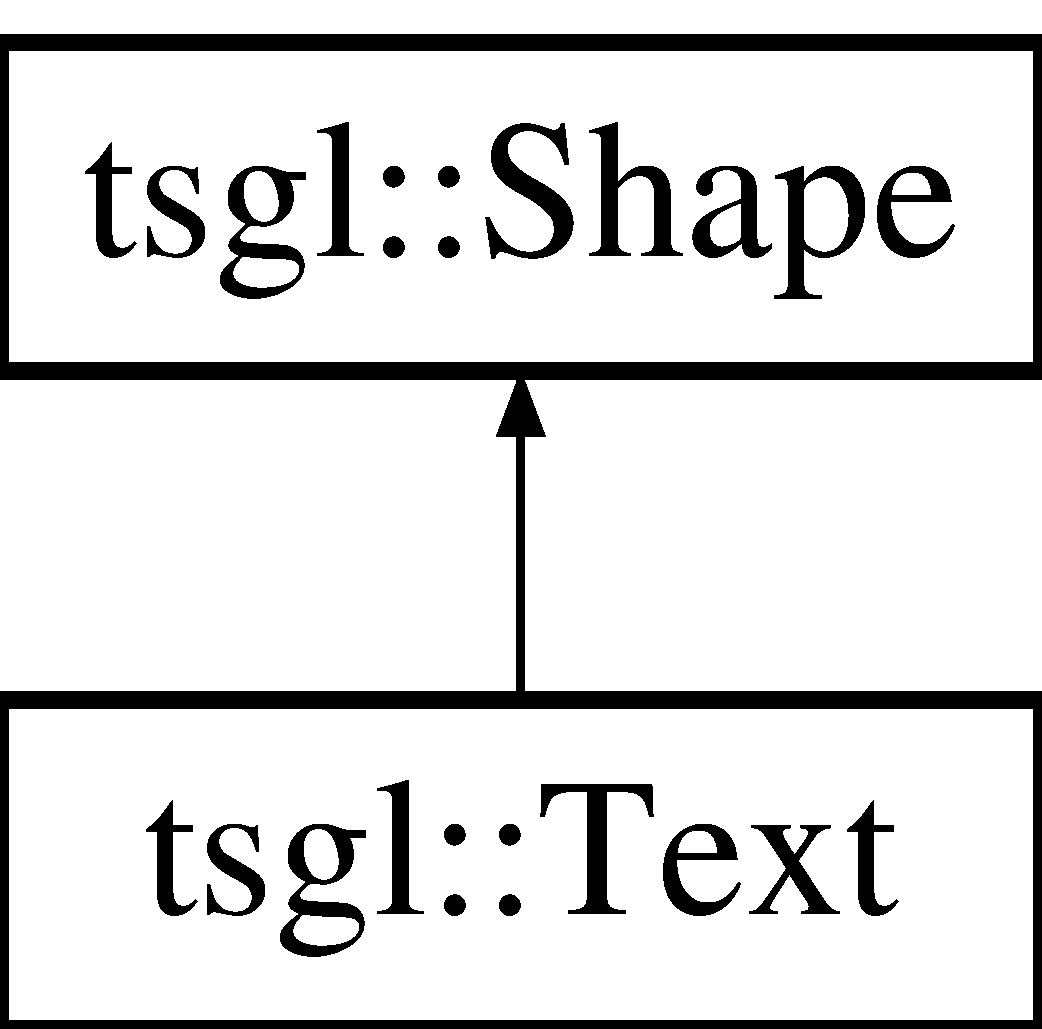
\includegraphics[height=2.000000cm]{classtsgl_1_1_text}
\end{center}
\end{figure}
\subsection*{\-Public \-Member \-Functions}
\begin{DoxyCompactItemize}
\item 
\hyperlink{classtsgl_1_1_text_ad1a6a77a4762f4420527457a7a5c24e7}{\-Text} (std\-::wstring text, \hyperlink{classtsgl_1_1_texture_handler}{\-Texture\-Handler} \&loader, int x, int y, unsigned int fontsize, const \hyperlink{structtsgl_1_1_color_float}{\-Color\-Float} \&color)
\begin{DoxyCompactList}\small\item\em \-Explicitly constructs a new \hyperlink{classtsgl_1_1_text}{\-Text} instance. \end{DoxyCompactList}\item 
void \hyperlink{classtsgl_1_1_text_a9dc47e4af682abfdab74e37b71f9fbde}{draw} ()
\begin{DoxyCompactList}\small\item\em \-Draw the \hyperlink{classtsgl_1_1_text}{\-Text}. \end{DoxyCompactList}\end{DoxyCompactItemize}


\subsection{\-Detailed \-Description}
\-Draw a string of text. 

\hyperlink{classtsgl_1_1_text}{\-Text} is a class for holding the data necessary for rendering a string of text. \begin{DoxyNote}{\-Note}
\hyperlink{classtsgl_1_1_text}{\-Text} is aligned by the upper-\/left corner. 

\-Fonts supported by \-Free\-Type are also supported. 
\end{DoxyNote}


\subsection{\-Constructor \& \-Destructor \-Documentation}
\hypertarget{classtsgl_1_1_text_ad1a6a77a4762f4420527457a7a5c24e7}{\index{tsgl\-::\-Text@{tsgl\-::\-Text}!\-Text@{\-Text}}
\index{\-Text@{\-Text}!tsgl::Text@{tsgl\-::\-Text}}
\subsubsection[{\-Text}]{\setlength{\rightskip}{0pt plus 5cm}{\bf tsgl\-::\-Text\-::\-Text} (
\begin{DoxyParamCaption}
\item[{std\-::wstring}]{text, }
\item[{{\bf \-Texture\-Handler} \&}]{loader, }
\item[{int}]{x, }
\item[{int}]{y, }
\item[{unsigned int}]{fontsize, }
\item[{const {\bf \-Color\-Float} \&}]{color}
\end{DoxyParamCaption}
)}}\label{classtsgl_1_1_text_ad1a6a77a4762f4420527457a7a5c24e7}


\-Explicitly constructs a new \hyperlink{classtsgl_1_1_text}{\-Text} instance. 

\-This is the constructor for the \hyperlink{classtsgl_1_1_text}{\-Text} class. 
\begin{DoxyParams}{\-Parameters}
{\em text} & \-The string to draw. \\
\hline
{\em loader} & \-A reference pointer to the \hyperlink{classtsgl_1_1_texture_handler}{\-Texture\-Handler} with which to load the font. \\
\hline
{\em x} & \-The x coordinate. \\
\hline
{\em y} & \-The y coordinate. \\
\hline
{\em fontsize} & \-The size of the text in pixels. \\
\hline
{\em color} & \-A reference to the \hyperlink{structtsgl_1_1_color_float}{\-Color\-Float} to use. \\
\hline
\end{DoxyParams}
\begin{DoxyReturn}{\-Returns}
\-A new \hyperlink{classtsgl_1_1_text}{\-Text} instance with the specified string, position, and color. 
\end{DoxyReturn}


\subsection{\-Member \-Function \-Documentation}
\hypertarget{classtsgl_1_1_text_a9dc47e4af682abfdab74e37b71f9fbde}{\index{tsgl\-::\-Text@{tsgl\-::\-Text}!draw@{draw}}
\index{draw@{draw}!tsgl::Text@{tsgl\-::\-Text}}
\subsubsection[{draw}]{\setlength{\rightskip}{0pt plus 5cm}void {\bf tsgl\-::\-Text\-::draw} (
\begin{DoxyParamCaption}
{}
\end{DoxyParamCaption}
)\hspace{0.3cm}{\ttfamily  \mbox{[}virtual\mbox{]}}}}\label{classtsgl_1_1_text_a9dc47e4af682abfdab74e37b71f9fbde}


\-Draw the \hyperlink{classtsgl_1_1_text}{\-Text}. 

\-This function actually draws the \hyperlink{classtsgl_1_1_text}{\-Text} to the \hyperlink{classtsgl_1_1_canvas}{\-Canvas}. 

\-Implements \hyperlink{classtsgl_1_1_shape_af78b1627b97d621824ce86db214e2402}{tsgl\-::\-Shape}.



\-The documentation for this class was generated from the following files\-:\begin{DoxyCompactItemize}
\item 
\-Text.\-h\item 
\-Text.\-cpp\end{DoxyCompactItemize}

\hypertarget{classtsgl_1_1_texture_handler}{\section{tsgl\-:\-:Texture\-Handler Class Reference}
\label{classtsgl_1_1_texture_handler}\index{tsgl\-::\-Texture\-Handler@{tsgl\-::\-Texture\-Handler}}
}


Handles saving, loading, and rendering of images and textures.  




{\ttfamily \#include $<$Texture\-Handler.\-h$>$}

\subsection*{Public Member Functions}
\begin{DoxyCompactItemize}
\item 
\hyperlink{classtsgl_1_1_texture_handler_a1a0db4cec4146d0735bc84cacfdaa5e5}{Texture\-Handler} ()
\begin{DoxyCompactList}\small\item\em Default \hyperlink{classtsgl_1_1_texture_handler}{Texture\-Handler} constructor method. \end{DoxyCompactList}\item 
\hyperlink{classtsgl_1_1_texture_handler_a64d0ef81c3c79edb06e23d62ca220c5d}{$\sim$\-Texture\-Handler} ()
\begin{DoxyCompactList}\small\item\em \hyperlink{classtsgl_1_1_texture_handler}{Texture\-Handler} destructor method. \end{DoxyCompactList}\item 
bool \hyperlink{classtsgl_1_1_texture_handler_a7f3103ea7f43f5a042609b443a748c88}{draw\-Text} (std\-::wstring text, unsigned int font\-\_\-size, float $\ast$vertices)
\begin{DoxyCompactList}\small\item\em Draws text. \end{DoxyCompactList}\item 
bool \hyperlink{classtsgl_1_1_texture_handler_a8f93300474b0a3a509ffbbbc753f3623}{load\-Font} (const std\-::string \&filename)
\begin{DoxyCompactList}\small\item\em Loads a font. \end{DoxyCompactList}\item 
G\-Ltexture \hyperlink{classtsgl_1_1_texture_handler_a0f760cedd2b6c1f72fe272efc5fbd047}{load\-Picture} (std\-::string filename, unsigned int \&width, unsigned int \&height, G\-Ltexture \&texture)
\begin{DoxyCompactList}\small\item\em Loads an image. \end{DoxyCompactList}\item 
bool \hyperlink{classtsgl_1_1_texture_handler_a29dc4554f9ba181abb5ed9fa45cc186f}{save\-Image\-To\-File} (std\-::string filename, G\-Lubyte $\ast$pixels, unsigned int width, unsigned int height) const 
\begin{DoxyCompactList}\small\item\em Saves an \hyperlink{classtsgl_1_1_image}{Image}. \end{DoxyCompactList}\end{DoxyCompactItemize}
\subsection*{Static Public Member Functions}
\begin{DoxyCompactItemize}
\item 
static void \hyperlink{classtsgl_1_1_texture_handler_ab88095c1d6bfc4181390165312298ff3}{get\-Dimensions} (std\-::string filename, int \&width, int \&height)
\begin{DoxyCompactList}\small\item\em Gets the dimensions of an image. \end{DoxyCompactList}\item 
\hypertarget{classtsgl_1_1_texture_handler_ac69f1c04f7ec17f475a5aac322f5ba6a}{static void \hyperlink{classtsgl_1_1_texture_handler_ac69f1c04f7ec17f475a5aac322f5ba6a}{run\-Tests} ()}\label{classtsgl_1_1_texture_handler_ac69f1c04f7ec17f475a5aac322f5ba6a}

\begin{DoxyCompactList}\small\item\em Runs the Unit tests for \hyperlink{classtsgl_1_1_texture_handler}{Texture\-Handler}. \end{DoxyCompactList}\end{DoxyCompactItemize}


\subsection{Detailed Description}
Handles saving, loading, and rendering of images and textures. 

\hyperlink{classtsgl_1_1_texture_handler}{Texture\-Handler} provides an interface for saving, loading, and rendering images and text to \hyperlink{classtsgl_1_1_canvas}{Canvas} and \hyperlink{classtsgl_1_1_cartesian_canvas}{Cartesian\-Canvas} through the use of G\-L\-Textures. 

\subsection{Constructor \& Destructor Documentation}
\hypertarget{classtsgl_1_1_texture_handler_a1a0db4cec4146d0735bc84cacfdaa5e5}{\index{tsgl\-::\-Texture\-Handler@{tsgl\-::\-Texture\-Handler}!Texture\-Handler@{Texture\-Handler}}
\index{Texture\-Handler@{Texture\-Handler}!tsgl::TextureHandler@{tsgl\-::\-Texture\-Handler}}
\subsubsection[{Texture\-Handler}]{\setlength{\rightskip}{0pt plus 5cm}tsgl\-::\-Texture\-Handler\-::\-Texture\-Handler (
\begin{DoxyParamCaption}
{}
\end{DoxyParamCaption}
)}}\label{classtsgl_1_1_texture_handler_a1a0db4cec4146d0735bc84cacfdaa5e5}


Default \hyperlink{classtsgl_1_1_texture_handler}{Texture\-Handler} constructor method. 

This is the default constructor for the\-Texture\-Handler \hyperlink{classtsgl_1_1_canvas}{Canvas} class. \begin{DoxyReturn}{Returns}
A new \hyperlink{classtsgl_1_1_texture_handler}{Texture\-Handler} instance. 
\end{DoxyReturn}
\hypertarget{classtsgl_1_1_texture_handler_a64d0ef81c3c79edb06e23d62ca220c5d}{\index{tsgl\-::\-Texture\-Handler@{tsgl\-::\-Texture\-Handler}!$\sim$\-Texture\-Handler@{$\sim$\-Texture\-Handler}}
\index{$\sim$\-Texture\-Handler@{$\sim$\-Texture\-Handler}!tsgl::TextureHandler@{tsgl\-::\-Texture\-Handler}}
\subsubsection[{$\sim$\-Texture\-Handler}]{\setlength{\rightskip}{0pt plus 5cm}tsgl\-::\-Texture\-Handler\-::$\sim$\-Texture\-Handler (
\begin{DoxyParamCaption}
{}
\end{DoxyParamCaption}
)}}\label{classtsgl_1_1_texture_handler_a64d0ef81c3c79edb06e23d62ca220c5d}


\hyperlink{classtsgl_1_1_texture_handler}{Texture\-Handler} destructor method. 

This is the destructor for the \hyperlink{classtsgl_1_1_texture_handler}{Texture\-Handler} class.

Frees up memory that was allocated to a \hyperlink{classtsgl_1_1_texture_handler}{Texture\-Handler} instance. 

\subsection{Member Function Documentation}
\hypertarget{classtsgl_1_1_texture_handler_a7f3103ea7f43f5a042609b443a748c88}{\index{tsgl\-::\-Texture\-Handler@{tsgl\-::\-Texture\-Handler}!draw\-Text@{draw\-Text}}
\index{draw\-Text@{draw\-Text}!tsgl::TextureHandler@{tsgl\-::\-Texture\-Handler}}
\subsubsection[{draw\-Text}]{\setlength{\rightskip}{0pt plus 5cm}bool tsgl\-::\-Texture\-Handler\-::draw\-Text (
\begin{DoxyParamCaption}
\item[{std\-::wstring}]{text, }
\item[{unsigned int}]{font\-\_\-size, }
\item[{float $\ast$}]{vertices}
\end{DoxyParamCaption}
)}}\label{classtsgl_1_1_texture_handler_a7f3103ea7f43f5a042609b443a748c88}


Draws text. 

Draws the text specified by its parameters onto a \hyperlink{classtsgl_1_1_canvas}{Canvas}. 
\begin{DoxyParams}{Parameters}
{\em text} & The U\-T\-F-\/8 encoded string of text to be drawn. \\
\hline
{\em font\-\_\-size} & The size of the text in pixels. \\
\hline
{\em vertices} & An array of vertex data for the bonding box of the text. \\
\hline
\end{DoxyParams}
\begin{DoxyNote}{Note}
{\ttfamily vertices} will be partially automatically set by \hyperlink{classtsgl_1_1_texture_handler_a7f3103ea7f43f5a042609b443a748c88}{draw\-Text()} itself in order to draw / kern the text properly, but the color, starting position, and texture coordinates will be left unchanged. 

If no font is loaded before calling this function, T\-S\-G\-L will attempt to locate a default font at {\itshape ../assets/freefont/\-Free\-Mono.ttf.} 
\end{DoxyNote}
\begin{DoxyReturn}{Returns}
True if successful, false otherwise. 
\end{DoxyReturn}
\begin{DoxyRefDesc}{Bug}
\item[\hyperlink{bug__bug000004}{Bug}]If the default font cannot be located, T\-S\-G\-L will crash. \end{DoxyRefDesc}


Referenced by tsgl\-::\-Text\-::draw().

\hypertarget{classtsgl_1_1_texture_handler_ab88095c1d6bfc4181390165312298ff3}{\index{tsgl\-::\-Texture\-Handler@{tsgl\-::\-Texture\-Handler}!get\-Dimensions@{get\-Dimensions}}
\index{get\-Dimensions@{get\-Dimensions}!tsgl::TextureHandler@{tsgl\-::\-Texture\-Handler}}
\subsubsection[{get\-Dimensions}]{\setlength{\rightskip}{0pt plus 5cm}void tsgl\-::\-Texture\-Handler\-::get\-Dimensions (
\begin{DoxyParamCaption}
\item[{std\-::string}]{filename, }
\item[{int \&}]{width, }
\item[{int \&}]{height}
\end{DoxyParamCaption}
)\hspace{0.3cm}{\ttfamily [static]}}}\label{classtsgl_1_1_texture_handler_ab88095c1d6bfc4181390165312298ff3}


Gets the dimensions of an image. 

Loads the header of a .png, .jpeg, or .bmp image to read their dimensions. 
\begin{DoxyParams}{Parameters}
{\em filename} & The file name of the picture. \\
\hline
{\em width} & A reference variable for holding the width of the picture. \\
\hline
{\em height} & A reference variable for holding the height of the picture. \\
\hline
\end{DoxyParams}
\begin{DoxyReturn}{Returns}
The texture that created from the loaded image. 
\end{DoxyReturn}


Referenced by tsgl\-::\-Image\-::\-Image().

\hypertarget{classtsgl_1_1_texture_handler_a8f93300474b0a3a509ffbbbc753f3623}{\index{tsgl\-::\-Texture\-Handler@{tsgl\-::\-Texture\-Handler}!load\-Font@{load\-Font}}
\index{load\-Font@{load\-Font}!tsgl::TextureHandler@{tsgl\-::\-Texture\-Handler}}
\subsubsection[{load\-Font}]{\setlength{\rightskip}{0pt plus 5cm}bool tsgl\-::\-Texture\-Handler\-::load\-Font (
\begin{DoxyParamCaption}
\item[{const std\-::string \&}]{filename}
\end{DoxyParamCaption}
)}}\label{classtsgl_1_1_texture_handler_a8f93300474b0a3a509ffbbbc753f3623}


Loads a font. 

Loads a font from the library given by {\ttfamily filename}. 
\begin{DoxyParams}{Parameters}
{\em filename} & The file name of the font to be loaded. \\
\hline
\end{DoxyParams}
\begin{DoxyWarning}{Warning}
If the font cannot be found then an error message is printed out. 

If the font library is not correctly installed then an error message is printed out. 

If the font is not supported then an error message is printed out. 
\end{DoxyWarning}
\begin{DoxyReturn}{Returns}
True if successful, false otherwise. 
\end{DoxyReturn}


Referenced by draw\-Text(), and tsgl\-::\-Canvas\-::set\-Font().

\hypertarget{classtsgl_1_1_texture_handler_a0f760cedd2b6c1f72fe272efc5fbd047}{\index{tsgl\-::\-Texture\-Handler@{tsgl\-::\-Texture\-Handler}!load\-Picture@{load\-Picture}}
\index{load\-Picture@{load\-Picture}!tsgl::TextureHandler@{tsgl\-::\-Texture\-Handler}}
\subsubsection[{load\-Picture}]{\setlength{\rightskip}{0pt plus 5cm}G\-Ltexture tsgl\-::\-Texture\-Handler\-::load\-Picture (
\begin{DoxyParamCaption}
\item[{std\-::string}]{filename, }
\item[{unsigned int \&}]{width, }
\item[{unsigned int \&}]{height, }
\item[{G\-Ltexture \&}]{texture}
\end{DoxyParamCaption}
)}}\label{classtsgl_1_1_texture_handler_a0f760cedd2b6c1f72fe272efc5fbd047}


Loads an image. 

Loads a .png, .jpeg, or .bmp image from a file. 
\begin{DoxyParams}{Parameters}
{\em filename} & The file name of the picture. \\
\hline
{\em width} & A reference variable for holding the width of the picture. \\
\hline
{\em height} & A reference variable for holding the height of the picture. \\
\hline
{\em texture} & A reference variable for holding the texture of the picture. (same as return value) \\
\hline
\end{DoxyParams}
\begin{DoxyReturn}{Returns}
The texture that created from the loaded image. 
\end{DoxyReturn}


Referenced by tsgl\-::\-Image\-::draw().

\hypertarget{classtsgl_1_1_texture_handler_a29dc4554f9ba181abb5ed9fa45cc186f}{\index{tsgl\-::\-Texture\-Handler@{tsgl\-::\-Texture\-Handler}!save\-Image\-To\-File@{save\-Image\-To\-File}}
\index{save\-Image\-To\-File@{save\-Image\-To\-File}!tsgl::TextureHandler@{tsgl\-::\-Texture\-Handler}}
\subsubsection[{save\-Image\-To\-File}]{\setlength{\rightskip}{0pt plus 5cm}bool tsgl\-::\-Texture\-Handler\-::save\-Image\-To\-File (
\begin{DoxyParamCaption}
\item[{std\-::string}]{filename, }
\item[{G\-Lubyte $\ast$}]{pixels, }
\item[{unsigned int}]{width, }
\item[{unsigned int}]{height}
\end{DoxyParamCaption}
) const}}\label{classtsgl_1_1_texture_handler_a29dc4554f9ba181abb5ed9fa45cc186f}


Saves an \hyperlink{classtsgl_1_1_image}{Image}. 

Saves an \hyperlink{classtsgl_1_1_image}{Image} to file that was captured from a \hyperlink{classtsgl_1_1_canvas}{Canvas} object. 
\begin{DoxyParams}{Parameters}
{\em filename} & The name of the file to save the \hyperlink{classtsgl_1_1_image}{Image} to. \\
\hline
{\em pixels} & The pixel data for the \hyperlink{classtsgl_1_1_image}{Image}. \\
\hline
{\em width} & The width of the \hyperlink{classtsgl_1_1_image}{Image}. \\
\hline
{\em height} & The height of the \hyperlink{classtsgl_1_1_image}{Image}. \\
\hline
\end{DoxyParams}
\begin{DoxyReturn}{Returns}
True if successful, false otherwise. 
\end{DoxyReturn}


The documentation for this class was generated from the following files\-:\begin{DoxyCompactItemize}
\item 
Texture\-Handler.\-h\item 
Texture\-Handler.\-cpp\end{DoxyCompactItemize}

\hypertarget{classtsgl_1_1_timer}{}\section{tsgl\+:\+:Timer Class Reference}
\label{classtsgl_1_1_timer}\index{tsgl\+::\+Timer@{tsgl\+::\+Timer}}


A class for various timing operations.  




{\ttfamily \#include $<$Timer.\+h$>$}

\subsection*{Public Member Functions}
\begin{DoxyCompactItemize}
\item 
\hyperlink{classtsgl_1_1_timer_abd022bb9ea6ddf5b69ff645ac8f5594d}{Timer} (double period)
\begin{DoxyCompactList}\small\item\em Default \hyperlink{classtsgl_1_1_timer}{Timer} constructor method. \end{DoxyCompactList}\item 
virtual \hyperlink{classtsgl_1_1_timer_a817d6b360361c744b13ff10377c130af}{$\sim$\+Timer} ()
\begin{DoxyCompactList}\small\item\em \hyperlink{classtsgl_1_1_timer}{Timer} destructor method. \end{DoxyCompactList}\item 
unsigned int \hyperlink{classtsgl_1_1_timer_aef59a24e4346529f69702f5742fa7612}{get\+Reps} () const 
\begin{DoxyCompactList}\small\item\em Gets the number of repetitions since starting the timer. \end{DoxyCompactList}\item 
double \hyperlink{classtsgl_1_1_timer_a063a0c8ff2a6f4aa920bc0cf44c18335}{get\+Time} () const 
\begin{DoxyCompactList}\small\item\em Gets the elapsed time since starting the timer. \end{DoxyCompactList}\item 
double \hyperlink{classtsgl_1_1_timer_a897a205bf63a7ebe6549167ea6b70698}{get\+Time\+Between\+Sleeps} () const 
\begin{DoxyCompactList}\small\item\em Get the elapsed time between sleeps. \end{DoxyCompactList}\item 
bool \hyperlink{classtsgl_1_1_timer_ac7c908b06a735f09841367c7067f44dd}{past\+Period} ()
\begin{DoxyCompactList}\small\item\em Check if the \hyperlink{classtsgl_1_1_timer}{Timer}\textquotesingle{}s period has elapsed. \end{DoxyCompactList}\item 
void \hyperlink{classtsgl_1_1_timer_a67a01c03c033c52056b7f1c733cd93e4}{reset} (double period=0)
\begin{DoxyCompactList}\small\item\em Reset the \hyperlink{classtsgl_1_1_timer}{Timer}. \end{DoxyCompactList}\item 
void \hyperlink{classtsgl_1_1_timer_a5c6e0dca6793d48c675e05b983da7f07}{sleep} (bool update=true)
\begin{DoxyCompactList}\small\item\em Sleeps the \hyperlink{classtsgl_1_1_timer}{Timer}\textquotesingle{}s current thread until its period elapses. \end{DoxyCompactList}\end{DoxyCompactItemize}
\subsection*{Static Public Member Functions}
\begin{DoxyCompactItemize}
\item 
static void \hyperlink{classtsgl_1_1_timer_ae8c5b39a6c5cae2a24abe2a298b05b64}{thread\+Sleep\+For} (double duration)
\begin{DoxyCompactList}\small\item\em Sleeps the current thread for the specified duration. \end{DoxyCompactList}\end{DoxyCompactItemize}


\subsection{Detailed Description}
A class for various timing operations. 

\hyperlink{classtsgl_1_1_timer}{Timer} provides a simple timer for timing, sleeping threads, and keeping track of the current rendering frame. 

\subsection{Constructor \& Destructor Documentation}
\hypertarget{classtsgl_1_1_timer_abd022bb9ea6ddf5b69ff645ac8f5594d}{}\index{tsgl\+::\+Timer@{tsgl\+::\+Timer}!Timer@{Timer}}
\index{Timer@{Timer}!tsgl\+::\+Timer@{tsgl\+::\+Timer}}
\subsubsection[{Timer}]{\setlength{\rightskip}{0pt plus 5cm}tsgl\+::\+Timer\+::\+Timer (
\begin{DoxyParamCaption}
\item[{double}]{period}
\end{DoxyParamCaption}
)}\label{classtsgl_1_1_timer_abd022bb9ea6ddf5b69ff645ac8f5594d}


Default \hyperlink{classtsgl_1_1_timer}{Timer} constructor method. 

This is the default constructor for the \hyperlink{classtsgl_1_1_timer}{Timer} class. 
\begin{DoxyParams}{Parameters}
{\em period} & Time in seconds specifying the maximum amount of time to sleep. \\
\hline
\end{DoxyParams}
\begin{DoxyReturn}{Returns}
A new \hyperlink{classtsgl_1_1_timer}{Timer} with the specified period. 
\end{DoxyReturn}
\hypertarget{classtsgl_1_1_timer_a817d6b360361c744b13ff10377c130af}{}\index{tsgl\+::\+Timer@{tsgl\+::\+Timer}!````~Timer@{$\sim$\+Timer}}
\index{````~Timer@{$\sim$\+Timer}!tsgl\+::\+Timer@{tsgl\+::\+Timer}}
\subsubsection[{$\sim$\+Timer}]{\setlength{\rightskip}{0pt plus 5cm}tsgl\+::\+Timer\+::$\sim$\+Timer (
\begin{DoxyParamCaption}
{}
\end{DoxyParamCaption}
)\hspace{0.3cm}{\ttfamily [virtual]}}\label{classtsgl_1_1_timer_a817d6b360361c744b13ff10377c130af}


\hyperlink{classtsgl_1_1_timer}{Timer} destructor method. 

This is the destructor for the \hyperlink{classtsgl_1_1_timer}{Timer} class.

Frees up memory that was allocated to a \hyperlink{classtsgl_1_1_timer}{Timer} instance. 

\subsection{Member Function Documentation}
\hypertarget{classtsgl_1_1_timer_aef59a24e4346529f69702f5742fa7612}{}\index{tsgl\+::\+Timer@{tsgl\+::\+Timer}!get\+Reps@{get\+Reps}}
\index{get\+Reps@{get\+Reps}!tsgl\+::\+Timer@{tsgl\+::\+Timer}}
\subsubsection[{get\+Reps}]{\setlength{\rightskip}{0pt plus 5cm}unsigned int tsgl\+::\+Timer\+::get\+Reps (
\begin{DoxyParamCaption}
{}
\end{DoxyParamCaption}
) const}\label{classtsgl_1_1_timer_aef59a24e4346529f69702f5742fa7612}


Gets the number of repetitions since starting the timer. 

\begin{DoxyReturn}{Returns}
The number of times the {\ttfamily period$<$/period$>$ has elapsed since the \hyperlink{classtsgl_1_1_timer}{Timer} has been started. }
\end{DoxyReturn}


Referenced by tsgl\+::\+Canvas\+::get\+Reps(), and past\+Period().

\hypertarget{classtsgl_1_1_timer_a063a0c8ff2a6f4aa920bc0cf44c18335}{}\index{tsgl\+::\+Timer@{tsgl\+::\+Timer}!get\+Time@{get\+Time}}
\index{get\+Time@{get\+Time}!tsgl\+::\+Timer@{tsgl\+::\+Timer}}
\subsubsection[{get\+Time}]{\setlength{\rightskip}{0pt plus 5cm}double tsgl\+::\+Timer\+::get\+Time (
\begin{DoxyParamCaption}
{}
\end{DoxyParamCaption}
) const}\label{classtsgl_1_1_timer_a063a0c8ff2a6f4aa920bc0cf44c18335}


Gets the elapsed time since starting the timer. 

\begin{DoxyReturn}{Returns}
The time in seconds since starting the \hyperlink{classtsgl_1_1_timer}{Timer}. 
\end{DoxyReturn}


Referenced by tsgl\+::\+Canvas\+::get\+Time().

\hypertarget{classtsgl_1_1_timer_a897a205bf63a7ebe6549167ea6b70698}{}\index{tsgl\+::\+Timer@{tsgl\+::\+Timer}!get\+Time\+Between\+Sleeps@{get\+Time\+Between\+Sleeps}}
\index{get\+Time\+Between\+Sleeps@{get\+Time\+Between\+Sleeps}!tsgl\+::\+Timer@{tsgl\+::\+Timer}}
\subsubsection[{get\+Time\+Between\+Sleeps}]{\setlength{\rightskip}{0pt plus 5cm}double tsgl\+::\+Timer\+::get\+Time\+Between\+Sleeps (
\begin{DoxyParamCaption}
{}
\end{DoxyParamCaption}
) const}\label{classtsgl_1_1_timer_a897a205bf63a7ebe6549167ea6b70698}


Get the elapsed time between sleeps. 

This function returns the time in seconds between returning from the last two calls to \hyperlink{classtsgl_1_1_timer_a5c6e0dca6793d48c675e05b983da7f07}{sleep()}. This should be the same as {\ttfamily period} in cases where the \hyperlink{classtsgl_1_1_timer}{Timer} is allowed to sleep. If the \hyperlink{classtsgl_1_1_timer}{Timer} has yet to sleep twice, \hyperlink{classtsgl_1_1_timer_a897a205bf63a7ebe6549167ea6b70698}{get\+Time\+Between\+Sleeps()} is undefined, but will most likely be less than 0. \begin{DoxyReturn}{Returns}
The time in seconds between the last two sleeps. 
\end{DoxyReturn}


Referenced by tsgl\+::\+Canvas\+::get\+Time\+Between\+Sleeps().

\hypertarget{classtsgl_1_1_timer_ac7c908b06a735f09841367c7067f44dd}{}\index{tsgl\+::\+Timer@{tsgl\+::\+Timer}!past\+Period@{past\+Period}}
\index{past\+Period@{past\+Period}!tsgl\+::\+Timer@{tsgl\+::\+Timer}}
\subsubsection[{past\+Period}]{\setlength{\rightskip}{0pt plus 5cm}bool tsgl\+::\+Timer\+::past\+Period (
\begin{DoxyParamCaption}
{}
\end{DoxyParamCaption}
)}\label{classtsgl_1_1_timer_ac7c908b06a735f09841367c7067f44dd}


Check if the \hyperlink{classtsgl_1_1_timer}{Timer}\textquotesingle{}s period has elapsed. 

This function returns whether the period of the \hyperlink{classtsgl_1_1_timer}{Timer} has elapsed since the last time the function was called. \begin{DoxyReturn}{Returns}
True if at least {\ttfamily period} seconds have elapsed since the last call, false otherwise. 
\end{DoxyReturn}
\hypertarget{classtsgl_1_1_timer_a67a01c03c033c52056b7f1c733cd93e4}{}\index{tsgl\+::\+Timer@{tsgl\+::\+Timer}!reset@{reset}}
\index{reset@{reset}!tsgl\+::\+Timer@{tsgl\+::\+Timer}}
\subsubsection[{reset}]{\setlength{\rightskip}{0pt plus 5cm}void tsgl\+::\+Timer\+::reset (
\begin{DoxyParamCaption}
\item[{double}]{period = {\ttfamily 0}}
\end{DoxyParamCaption}
)}\label{classtsgl_1_1_timer_a67a01c03c033c52056b7f1c733cd93e4}


Reset the \hyperlink{classtsgl_1_1_timer}{Timer}. 

This function resets the starting time, repetitions, and period of the timer. 
\begin{DoxyParams}{Parameters}
{\em period} & The new period for the \hyperlink{classtsgl_1_1_timer}{Timer}. Setting this less than or equal to 0 will keep the current period. \\
\hline
\end{DoxyParams}


Referenced by tsgl\+::\+Canvas\+::reset(), and Timer().

\hypertarget{classtsgl_1_1_timer_a5c6e0dca6793d48c675e05b983da7f07}{}\index{tsgl\+::\+Timer@{tsgl\+::\+Timer}!sleep@{sleep}}
\index{sleep@{sleep}!tsgl\+::\+Timer@{tsgl\+::\+Timer}}
\subsubsection[{sleep}]{\setlength{\rightskip}{0pt plus 5cm}void tsgl\+::\+Timer\+::sleep (
\begin{DoxyParamCaption}
\item[{bool}]{update = {\ttfamily true}}
\end{DoxyParamCaption}
)}\label{classtsgl_1_1_timer_a5c6e0dca6793d48c675e05b983da7f07}


Sleeps the \hyperlink{classtsgl_1_1_timer}{Timer}\textquotesingle{}s current thread until its period elapses. 

This function tells the currently executing thread to sleep until the rest of the \hyperlink{classtsgl_1_1_timer}{Timer} instance\textquotesingle{}s remaining period expires.

If the \hyperlink{classtsgl_1_1_timer}{Timer}\textquotesingle{}s period has elapsed since last call, the thread will continue execution normally until the next call to \hyperlink{classtsgl_1_1_timer_a5c6e0dca6793d48c675e05b983da7f07}{sleep()}. 
\begin{DoxyParams}{Parameters}
{\em update} & Whether to update the timer\textquotesingle{}s last\+\_\+rep status or not. \\
\hline
\end{DoxyParams}
\begin{DoxyNote}{Note}
This function does not guarantee the thread will resume immediately after the time expires. Depending on your O\+S, the thread may sleep for longer. 
\end{DoxyNote}
\begin{DoxySeeAlso}{See also}
\hyperlink{classtsgl_1_1_timer_a897a205bf63a7ebe6549167ea6b70698}{get\+Time\+Between\+Sleeps()}, to get the actual elapsed time between sleeps. 
\end{DoxySeeAlso}


Referenced by tsgl\+::\+Canvas\+::sleep().

\hypertarget{classtsgl_1_1_timer_ae8c5b39a6c5cae2a24abe2a298b05b64}{}\index{tsgl\+::\+Timer@{tsgl\+::\+Timer}!thread\+Sleep\+For@{thread\+Sleep\+For}}
\index{thread\+Sleep\+For@{thread\+Sleep\+For}!tsgl\+::\+Timer@{tsgl\+::\+Timer}}
\subsubsection[{thread\+Sleep\+For}]{\setlength{\rightskip}{0pt plus 5cm}void tsgl\+::\+Timer\+::thread\+Sleep\+For (
\begin{DoxyParamCaption}
\item[{double}]{duration}
\end{DoxyParamCaption}
)\hspace{0.3cm}{\ttfamily [static]}}\label{classtsgl_1_1_timer_ae8c5b39a6c5cae2a24abe2a298b05b64}


Sleeps the current thread for the specified duration. 

This function tells the currently executing thread to sleep for {\ttfamily duration} seconds. \begin{DoxyNote}{Note}
This function does not guarantee the thread will resume immediately after {\ttfamily duration} expires. Depending on your O\+S, the thread may sleep for longer. 
\end{DoxyNote}


The documentation for this class was generated from the following files\+:\begin{DoxyCompactItemize}
\item 
Timer.\+h\item 
Timer.\+cpp\end{DoxyCompactItemize}

\hypertarget{classtsgl_1_1_triangle}{}\section{tsgl\+:\+:Triangle Class Reference}
\label{classtsgl_1_1_triangle}\index{tsgl\+::\+Triangle@{tsgl\+::\+Triangle}}


Draw a simple \hyperlink{classtsgl_1_1_triangle}{Triangle}.  




{\ttfamily \#include $<$Triangle.\+h$>$}

Inheritance diagram for tsgl\+:\+:Triangle\+:\begin{figure}[H]
\begin{center}
\leavevmode
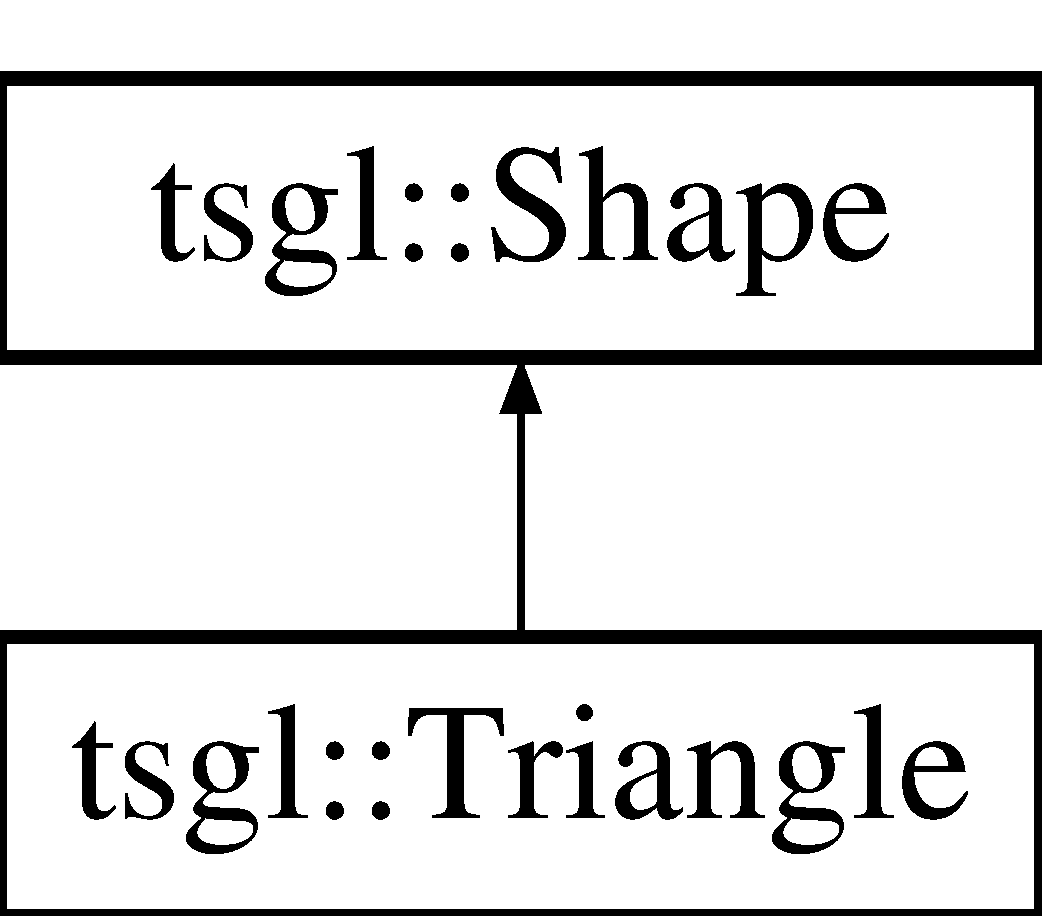
\includegraphics[height=2.000000cm]{classtsgl_1_1_triangle}
\end{center}
\end{figure}
\subsection*{Public Member Functions}
\begin{DoxyCompactItemize}
\item 
\hyperlink{classtsgl_1_1_triangle_a5ee7f4735479c2692d1d6a2d22ba5c28}{Triangle} (int x1, int y1, int x2, int y2, int x3, int y3, const \hyperlink{structtsgl_1_1_color_float}{Color\+Float} \&color)
\begin{DoxyCompactList}\small\item\em Explicitly constructs a new \hyperlink{classtsgl_1_1_triangle}{Triangle}. \end{DoxyCompactList}\item 
void \hyperlink{classtsgl_1_1_triangle_a83b30f9f7c800146fa900d32a58fa0c7}{draw} ()
\begin{DoxyCompactList}\small\item\em Draw the \hyperlink{classtsgl_1_1_triangle}{Triangle}. \end{DoxyCompactList}\end{DoxyCompactItemize}
\subsection*{Additional Inherited Members}


\subsection{Detailed Description}
Draw a simple \hyperlink{classtsgl_1_1_triangle}{Triangle}. 

\hyperlink{classtsgl_1_1_triangle}{Triangle} is a class for holding vertex data for a simple triangle. 

\subsection{Constructor \& Destructor Documentation}
\hypertarget{classtsgl_1_1_triangle_a5ee7f4735479c2692d1d6a2d22ba5c28}{}\index{tsgl\+::\+Triangle@{tsgl\+::\+Triangle}!Triangle@{Triangle}}
\index{Triangle@{Triangle}!tsgl\+::\+Triangle@{tsgl\+::\+Triangle}}
\subsubsection[{Triangle}]{\setlength{\rightskip}{0pt plus 5cm}tsgl\+::\+Triangle\+::\+Triangle (
\begin{DoxyParamCaption}
\item[{int}]{x1, }
\item[{int}]{y1, }
\item[{int}]{x2, }
\item[{int}]{y2, }
\item[{int}]{x3, }
\item[{int}]{y3, }
\item[{const {\bf Color\+Float} \&}]{color}
\end{DoxyParamCaption}
)}\label{classtsgl_1_1_triangle_a5ee7f4735479c2692d1d6a2d22ba5c28}


Explicitly constructs a new \hyperlink{classtsgl_1_1_triangle}{Triangle}. 

This is the constructor for the \hyperlink{classtsgl_1_1_triangle}{Triangle} class. 
\begin{DoxyParams}{Parameters}
{\em x1} & The x coordinate of the first endpoint. \\
\hline
{\em y1} & The y coordinate of the first endpoint. \\
\hline
{\em x2} & The x coordinate of the second endpoint. \\
\hline
{\em y2} & The y coordinate of the second endpoint. \\
\hline
{\em x3} & The x coordinate of the third endpoint. \\
\hline
{\em y3} & The y coordinate of the third endpoint. \\
\hline
{\em color} & The color of the \hyperlink{classtsgl_1_1_triangle}{Triangle}. \\
\hline
\end{DoxyParams}
\begin{DoxyReturn}{Returns}
A new \hyperlink{classtsgl_1_1_triangle}{Triangle} with the specified vertices and color. 
\end{DoxyReturn}


\subsection{Member Function Documentation}
\hypertarget{classtsgl_1_1_triangle_a83b30f9f7c800146fa900d32a58fa0c7}{}\index{tsgl\+::\+Triangle@{tsgl\+::\+Triangle}!draw@{draw}}
\index{draw@{draw}!tsgl\+::\+Triangle@{tsgl\+::\+Triangle}}
\subsubsection[{draw}]{\setlength{\rightskip}{0pt plus 5cm}void tsgl\+::\+Triangle\+::draw (
\begin{DoxyParamCaption}
{}
\end{DoxyParamCaption}
)\hspace{0.3cm}{\ttfamily [virtual]}}\label{classtsgl_1_1_triangle_a83b30f9f7c800146fa900d32a58fa0c7}


Draw the \hyperlink{classtsgl_1_1_triangle}{Triangle}. 

This function actually draws the \hyperlink{classtsgl_1_1_triangle}{Triangle} to the \hyperlink{classtsgl_1_1_canvas}{Canvas}. 

Implements \hyperlink{classtsgl_1_1_shape_af78b1627b97d621824ce86db214e2402}{tsgl\+::\+Shape}.



The documentation for this class was generated from the following files\+:\begin{DoxyCompactItemize}
\item 
Triangle.\+h\item 
Triangle.\+cpp\end{DoxyCompactItemize}

\hypertarget{classtsgl_1_1_triangle_strip}{}\section{tsgl\+:\+:Triangle\+Strip Class Reference}
\label{classtsgl_1_1_triangle_strip}\index{tsgl\+::\+Triangle\+Strip@{tsgl\+::\+Triangle\+Strip}}


Draw an arbitrary triangle strip with colored vertices.  




{\ttfamily \#include $<$Triangle\+Strip.\+h$>$}

Inheritance diagram for tsgl\+:\+:Triangle\+Strip\+:\begin{figure}[H]
\begin{center}
\leavevmode
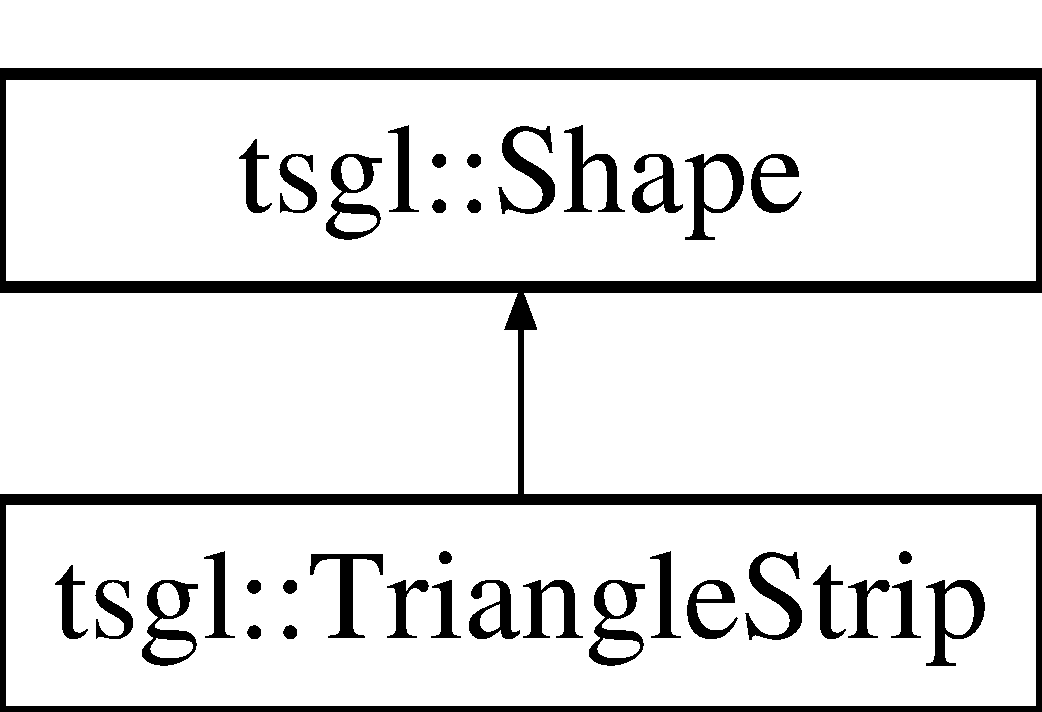
\includegraphics[height=2.000000cm]{classtsgl_1_1_triangle_strip}
\end{center}
\end{figure}
\subsection*{Public Member Functions}
\begin{DoxyCompactItemize}
\item 
\hyperlink{classtsgl_1_1_triangle_strip_ad68084f6e384f9faf86f2de673de0502}{Triangle\+Strip} (int num\+Vertices)
\begin{DoxyCompactList}\small\item\em Explicitly construct a new \hyperlink{classtsgl_1_1_triangle_strip}{Triangle\+Strip}. \end{DoxyCompactList}\item 
\hyperlink{classtsgl_1_1_triangle_strip_aab2dc311f7c7df4712c901878c048d96}{$\sim$\+Triangle\+Strip} ()
\begin{DoxyCompactList}\small\item\em Destroys a \hyperlink{classtsgl_1_1_triangle_strip}{Triangle\+Strip} object. \end{DoxyCompactList}\item 
void \hyperlink{classtsgl_1_1_triangle_strip_ad1773092235f2477bae32f10387874ef}{add\+Vertex} (int x, int y, const \hyperlink{structtsgl_1_1_color_float}{Color\+Float} \&color)
\begin{DoxyCompactList}\small\item\em Adds another vertex to a \hyperlink{classtsgl_1_1_triangle_strip}{Triangle\+Strip}. \end{DoxyCompactList}\item 
void \hyperlink{classtsgl_1_1_triangle_strip_a7a984063f85c8b6ab61bd6e989d38920}{draw} ()
\begin{DoxyCompactList}\small\item\em Draw the \hyperlink{classtsgl_1_1_triangle_strip}{Triangle\+Strip}. \end{DoxyCompactList}\end{DoxyCompactItemize}
\subsection*{Additional Inherited Members}


\subsection{Detailed Description}
Draw an arbitrary triangle strip with colored vertices. 

\hyperlink{classtsgl_1_1_triangle_strip}{Triangle\+Strip} is a class for holding vertex data for a triangle strip with colored vertices.

Vertices are drawn in triangle strip format, where the first three vertices make up the first triangle, the next vertex plus the previous two make up the second triangle, and so on.

This method is optimized for long lists and offers a marked improvement over drawing individual \hyperlink{classtsgl_1_1_triangle}{Triangle} instances. \begin{DoxyNote}{Note}
The \hyperlink{classtsgl_1_1_triangle_strip_ad1773092235f2477bae32f10387874ef}{add\+Vertex()} method must be called the same number of times as specified in the constructor. 

Calling \hyperlink{classtsgl_1_1_triangle_strip_ad1773092235f2477bae32f10387874ef}{add\+Vertex()} after all vertices have been added will do nothing. 

Calling \hyperlink{classtsgl_1_1_triangle_strip_a7a984063f85c8b6ab61bd6e989d38920}{draw()} before all vertices have been added will do nothing. 
\end{DoxyNote}


\subsection{Constructor \& Destructor Documentation}
\hypertarget{classtsgl_1_1_triangle_strip_ad68084f6e384f9faf86f2de673de0502}{}\index{tsgl\+::\+Triangle\+Strip@{tsgl\+::\+Triangle\+Strip}!Triangle\+Strip@{Triangle\+Strip}}
\index{Triangle\+Strip@{Triangle\+Strip}!tsgl\+::\+Triangle\+Strip@{tsgl\+::\+Triangle\+Strip}}
\subsubsection[{Triangle\+Strip}]{\setlength{\rightskip}{0pt plus 5cm}tsgl\+::\+Triangle\+Strip\+::\+Triangle\+Strip (
\begin{DoxyParamCaption}
\item[{int}]{num\+Vertices}
\end{DoxyParamCaption}
)}\label{classtsgl_1_1_triangle_strip_ad68084f6e384f9faf86f2de673de0502}


Explicitly construct a new \hyperlink{classtsgl_1_1_triangle_strip}{Triangle\+Strip}. 

Explicit constructor for a \hyperlink{classtsgl_1_1_triangle_strip}{Triangle\+Strip} object. 
\begin{DoxyParams}{Parameters}
{\em num\+Vertices} & The number of vertices the complete \hyperlink{classtsgl_1_1_triangle_strip}{Triangle\+Strip} will have. \\
\hline
\end{DoxyParams}
\begin{DoxyWarning}{Warning}
An invariant is held where if v is less than 3 then an error message is given. 
\end{DoxyWarning}
\begin{DoxyReturn}{Returns}
A new \hyperlink{classtsgl_1_1_triangle_strip}{Triangle\+Strip} with a buffer for storing the specified numbered of vertices. 
\end{DoxyReturn}
\hypertarget{classtsgl_1_1_triangle_strip_aab2dc311f7c7df4712c901878c048d96}{}\index{tsgl\+::\+Triangle\+Strip@{tsgl\+::\+Triangle\+Strip}!````~Triangle\+Strip@{$\sim$\+Triangle\+Strip}}
\index{````~Triangle\+Strip@{$\sim$\+Triangle\+Strip}!tsgl\+::\+Triangle\+Strip@{tsgl\+::\+Triangle\+Strip}}
\subsubsection[{$\sim$\+Triangle\+Strip}]{\setlength{\rightskip}{0pt plus 5cm}tsgl\+::\+Triangle\+Strip\+::$\sim$\+Triangle\+Strip (
\begin{DoxyParamCaption}
{}
\end{DoxyParamCaption}
)}\label{classtsgl_1_1_triangle_strip_aab2dc311f7c7df4712c901878c048d96}


Destroys a \hyperlink{classtsgl_1_1_triangle_strip}{Triangle\+Strip} object. 

Destructor for a \hyperlink{classtsgl_1_1_triangle_strip}{Triangle\+Strip} object.

Frees up memory that has been allocated to a \hyperlink{classtsgl_1_1_triangle_strip}{Triangle\+Strip} object. 

\subsection{Member Function Documentation}
\hypertarget{classtsgl_1_1_triangle_strip_ad1773092235f2477bae32f10387874ef}{}\index{tsgl\+::\+Triangle\+Strip@{tsgl\+::\+Triangle\+Strip}!add\+Vertex@{add\+Vertex}}
\index{add\+Vertex@{add\+Vertex}!tsgl\+::\+Triangle\+Strip@{tsgl\+::\+Triangle\+Strip}}
\subsubsection[{add\+Vertex}]{\setlength{\rightskip}{0pt plus 5cm}void tsgl\+::\+Triangle\+Strip\+::add\+Vertex (
\begin{DoxyParamCaption}
\item[{int}]{x, }
\item[{int}]{y, }
\item[{const {\bf Color\+Float} \&}]{color}
\end{DoxyParamCaption}
)}\label{classtsgl_1_1_triangle_strip_ad1773092235f2477bae32f10387874ef}


Adds another vertex to a \hyperlink{classtsgl_1_1_triangle_strip}{Triangle\+Strip}. 

This function initializes the next vertex in the \hyperlink{classtsgl_1_1_polyline}{Polyline} and adds it to a \hyperlink{classtsgl_1_1_triangle_strip}{Triangle\+Strip} buffer. 
\begin{DoxyParams}{Parameters}
{\em x} & The x position of the vertex. \\
\hline
{\em y} & The y position of the vertex. \\
\hline
{\em color} & The reference variable to a color of the vertex. \\
\hline
\end{DoxyParams}
\begin{DoxyNote}{Note}
This function does nothing if the vertex buffer is already full. 

A message will be given to show when the vertex buffer is full. 
\end{DoxyNote}


Referenced by tsgl\+::\+Canvas\+::draw\+Triangle\+Strip().

\hypertarget{classtsgl_1_1_triangle_strip_a7a984063f85c8b6ab61bd6e989d38920}{}\index{tsgl\+::\+Triangle\+Strip@{tsgl\+::\+Triangle\+Strip}!draw@{draw}}
\index{draw@{draw}!tsgl\+::\+Triangle\+Strip@{tsgl\+::\+Triangle\+Strip}}
\subsubsection[{draw}]{\setlength{\rightskip}{0pt plus 5cm}void tsgl\+::\+Triangle\+Strip\+::draw (
\begin{DoxyParamCaption}
{}
\end{DoxyParamCaption}
)\hspace{0.3cm}{\ttfamily [virtual]}}\label{classtsgl_1_1_triangle_strip_a7a984063f85c8b6ab61bd6e989d38920}


Draw the \hyperlink{classtsgl_1_1_triangle_strip}{Triangle\+Strip}. 

This function actually draws the \hyperlink{classtsgl_1_1_triangle_strip}{Triangle\+Strip} to the \hyperlink{classtsgl_1_1_canvas}{Canvas}. \begin{DoxyNote}{Note}
This function does nothing if the vertex buffer is not yet full. 

A message will be given to show if the \hyperlink{classtsgl_1_1_triangle_strip}{Triangle\+Strip} is {\itshape N\+O\+T} ready to be drawn (vertex buffer = not full). 

Implemented inherited abstract method from \hyperlink{classtsgl_1_1_shape}{Shape} class. 
\end{DoxyNote}


Implements \hyperlink{classtsgl_1_1_shape_af78b1627b97d621824ce86db214e2402}{tsgl\+::\+Shape}.



The documentation for this class was generated from the following files\+:\begin{DoxyCompactItemize}
\item 
Triangle\+Strip.\+h\item 
Triangle\+Strip.\+cpp\end{DoxyCompactItemize}

\hypertarget{classtsgl_1_1_visual_task_queue}{}\section{tsgl\+:\+:Visual\+Task\+Queue Class Reference}
\label{classtsgl_1_1_visual_task_queue}\index{tsgl\+::\+Visual\+Task\+Queue@{tsgl\+::\+Visual\+Task\+Queue}}


Provides a a visualization tool for a parallel queue of elements.  




{\ttfamily \#include $<$Visual\+Task\+Queue.\+h$>$}

\subsection*{Public Member Functions}
\begin{DoxyCompactItemize}
\item 
\hyperlink{classtsgl_1_1_visual_task_queue_ad82aabf35ec367b2b0c5894999f5e76e}{Visual\+Task\+Queue} (int elements, int side\+Length=12, float aspect=1.\+0f, int spacing=2, int border\+Length=8)
\begin{DoxyCompactList}\small\item\em Default \hyperlink{classtsgl_1_1_visual_task_queue}{Visual\+Task\+Queue} constructor method. \end{DoxyCompactList}\item 
\hyperlink{classtsgl_1_1_visual_task_queue_ae961a57508ba1d38570d1431c4367a09}{$\sim$\+Visual\+Task\+Queue} ()
\begin{DoxyCompactList}\small\item\em \hyperlink{classtsgl_1_1_visual_task_queue}{Visual\+Task\+Queue} destructor method. \end{DoxyCompactList}\item 
void \hyperlink{classtsgl_1_1_visual_task_queue_a7153e63b78fc257f162410c3e55e13dc}{show\+Legend} (int threads=-\/1)
\begin{DoxyCompactList}\small\item\em Shows a key/legend for the \hyperlink{classtsgl_1_1_visual_task_queue}{Visual\+Task\+Queue}. \end{DoxyCompactList}\item 
void \hyperlink{classtsgl_1_1_visual_task_queue_a2fc5733a57213a6eee116408738851fc}{update} (int index, V\+Q\+State state)
\begin{DoxyCompactList}\small\item\em Updates the state of the \hyperlink{classtsgl_1_1_visual_task_queue}{Visual\+Task\+Queue}. \end{DoxyCompactList}\item 
void \hyperlink{classtsgl_1_1_visual_task_queue_a1cd23a5361c0209ac950db6afcd68a19}{reset} ()
\begin{DoxyCompactList}\small\item\em Resets all of the elements in the \hyperlink{classtsgl_1_1_visual_task_queue}{Visual\+Task\+Queue}. \end{DoxyCompactList}\item 
void \hyperlink{classtsgl_1_1_visual_task_queue_a7340d211424a9f947152fed22cce4d79}{close} ()
\begin{DoxyCompactList}\small\item\em Closes the visual queue. \end{DoxyCompactList}\end{DoxyCompactItemize}


\subsection{Detailed Description}
Provides a a visualization tool for a parallel queue of elements. 

\hyperlink{classtsgl_1_1_visual_task_queue}{Visual\+Task\+Queue} is a self-\/contained \hyperlink{classtsgl_1_1_canvas}{Canvas} intended to help visualize the progress of a parallel queue of taks or elements.

Given a maximum queue length of {\ttfamily N} elements, a \hyperlink{classtsgl_1_1_visual_task_queue}{Visual\+Task\+Queue} will display {\ttfamily N} rectangles on its internal \hyperlink{classtsgl_1_1_canvas}{Canvas}. These rectangles can be in one of three states\+: cleared, running, or finished. Cleared elements are always displayed in white, whereas running elements are displayed in a darker shade of the current thread\textquotesingle{}s color, and finished elements are displayed in a lighter shade of the color of the thread the completed the element. 

\subsection{Constructor \& Destructor Documentation}
\hypertarget{classtsgl_1_1_visual_task_queue_ad82aabf35ec367b2b0c5894999f5e76e}{}\index{tsgl\+::\+Visual\+Task\+Queue@{tsgl\+::\+Visual\+Task\+Queue}!Visual\+Task\+Queue@{Visual\+Task\+Queue}}
\index{Visual\+Task\+Queue@{Visual\+Task\+Queue}!tsgl\+::\+Visual\+Task\+Queue@{tsgl\+::\+Visual\+Task\+Queue}}
\subsubsection[{Visual\+Task\+Queue}]{\setlength{\rightskip}{0pt plus 5cm}tsgl\+::\+Visual\+Task\+Queue\+::\+Visual\+Task\+Queue (
\begin{DoxyParamCaption}
\item[{int}]{elements, }
\item[{int}]{side\+Length = {\ttfamily 12}, }
\item[{float}]{aspect = {\ttfamily 1.0f}, }
\item[{int}]{spacing = {\ttfamily 2}, }
\item[{int}]{border\+Length = {\ttfamily 8}}
\end{DoxyParamCaption}
)}\label{classtsgl_1_1_visual_task_queue_ad82aabf35ec367b2b0c5894999f5e76e}


Default \hyperlink{classtsgl_1_1_visual_task_queue}{Visual\+Task\+Queue} constructor method. 

This is the default constructor for the \hyperlink{classtsgl_1_1_visual_task_queue}{Visual\+Task\+Queue} class. 
\begin{DoxyParams}{Parameters}
{\em elements} & The maximum number of elements to be drawn on the \hyperlink{classtsgl_1_1_visual_task_queue}{Visual\+Task\+Queue}. Setting this to higher than the actual number of elements may result in some unused, empty rectangle. Setting this to lower than the actual number of elements may result in some rectangles being drawn off the \hyperlink{classtsgl_1_1_visual_task_queue}{Visual\+Task\+Queue} \hyperlink{classtsgl_1_1_canvas}{Canvas}. \\
\hline
{\em side\+Length} & The side length in pixels of the task rectangles to be drawn on the \hyperlink{classtsgl_1_1_visual_task_queue}{Visual\+Task\+Queue} \hyperlink{classtsgl_1_1_canvas}{Canvas}. \\
\hline
{\em aspec} & The approximate aspect ratio of height/width for the \hyperlink{classtsgl_1_1_visual_task_queue}{Visual\+Task\+Queue} \hyperlink{classtsgl_1_1_canvas}{Canvas}. \\
\hline
{\em spacing} & The space in pixels between the rectangles representing elements in the \hyperlink{classtsgl_1_1_visual_task_queue}{Visual\+Task\+Queue}. \\
\hline
{\em border\+Length} & The space in pixels between the outer \hyperlink{classtsgl_1_1_visual_task_queue}{Visual\+Task\+Queue} rectangles and the border of the \hyperlink{classtsgl_1_1_visual_task_queue}{Visual\+Task\+Queue} \hyperlink{classtsgl_1_1_canvas}{Canvas}. \\
\hline
\end{DoxyParams}
\begin{DoxyReturn}{Returns}
A new \hyperlink{classtsgl_1_1_visual_task_queue}{Visual\+Task\+Queue} with the specified maximum number of elements, rectangle side length, approximate aspect ratio, spacing between rectangles, and spacing around the borders. 
\end{DoxyReturn}
\hypertarget{classtsgl_1_1_visual_task_queue_ae961a57508ba1d38570d1431c4367a09}{}\index{tsgl\+::\+Visual\+Task\+Queue@{tsgl\+::\+Visual\+Task\+Queue}!````~Visual\+Task\+Queue@{$\sim$\+Visual\+Task\+Queue}}
\index{````~Visual\+Task\+Queue@{$\sim$\+Visual\+Task\+Queue}!tsgl\+::\+Visual\+Task\+Queue@{tsgl\+::\+Visual\+Task\+Queue}}
\subsubsection[{$\sim$\+Visual\+Task\+Queue}]{\setlength{\rightskip}{0pt plus 5cm}tsgl\+::\+Visual\+Task\+Queue\+::$\sim$\+Visual\+Task\+Queue (
\begin{DoxyParamCaption}
{}
\end{DoxyParamCaption}
)}\label{classtsgl_1_1_visual_task_queue_ae961a57508ba1d38570d1431c4367a09}


\hyperlink{classtsgl_1_1_visual_task_queue}{Visual\+Task\+Queue} destructor method. 

This is the destructor for the \hyperlink{classtsgl_1_1_visual_task_queue}{Visual\+Task\+Queue} class.

Frees up memory that was allocated to a \hyperlink{classtsgl_1_1_visual_task_queue}{Visual\+Task\+Queue} instance. 

\subsection{Member Function Documentation}
\hypertarget{classtsgl_1_1_visual_task_queue_a7340d211424a9f947152fed22cce4d79}{}\index{tsgl\+::\+Visual\+Task\+Queue@{tsgl\+::\+Visual\+Task\+Queue}!close@{close}}
\index{close@{close}!tsgl\+::\+Visual\+Task\+Queue@{tsgl\+::\+Visual\+Task\+Queue}}
\subsubsection[{close}]{\setlength{\rightskip}{0pt plus 5cm}void tsgl\+::\+Visual\+Task\+Queue\+::close (
\begin{DoxyParamCaption}
{}
\end{DoxyParamCaption}
)}\label{classtsgl_1_1_visual_task_queue_a7340d211424a9f947152fed22cce4d79}


Closes the visual queue. 

This function closes and destroys the internal \hyperlink{classtsgl_1_1_canvas}{Canvas} created by the \hyperlink{classtsgl_1_1_visual_task_queue}{Visual\+Task\+Queue}. \begin{DoxyWarning}{Warning}
{\bfseries  Do not attempt to \hyperlink{classtsgl_1_1_visual_task_queue_a1cd23a5361c0209ac950db6afcd68a19}{reset()} or \hyperlink{classtsgl_1_1_visual_task_queue_a2fc5733a57213a6eee116408738851fc}{update()} the \hyperlink{classtsgl_1_1_visual_task_queue}{Visual\+Task\+Queue} after closing it.} 
\end{DoxyWarning}
\hypertarget{classtsgl_1_1_visual_task_queue_a1cd23a5361c0209ac950db6afcd68a19}{}\index{tsgl\+::\+Visual\+Task\+Queue@{tsgl\+::\+Visual\+Task\+Queue}!reset@{reset}}
\index{reset@{reset}!tsgl\+::\+Visual\+Task\+Queue@{tsgl\+::\+Visual\+Task\+Queue}}
\subsubsection[{reset}]{\setlength{\rightskip}{0pt plus 5cm}void tsgl\+::\+Visual\+Task\+Queue\+::reset (
\begin{DoxyParamCaption}
{}
\end{DoxyParamCaption}
)}\label{classtsgl_1_1_visual_task_queue_a1cd23a5361c0209ac950db6afcd68a19}


Resets all of the elements in the \hyperlink{classtsgl_1_1_visual_task_queue}{Visual\+Task\+Queue}. 

This function tells \hyperlink{classtsgl_1_1_visual_task_queue}{Visual\+Task\+Queue} to clear the state information of all of the elements. 

Referenced by Visual\+Task\+Queue().

\hypertarget{classtsgl_1_1_visual_task_queue_a7153e63b78fc257f162410c3e55e13dc}{}\index{tsgl\+::\+Visual\+Task\+Queue@{tsgl\+::\+Visual\+Task\+Queue}!show\+Legend@{show\+Legend}}
\index{show\+Legend@{show\+Legend}!tsgl\+::\+Visual\+Task\+Queue@{tsgl\+::\+Visual\+Task\+Queue}}
\subsubsection[{show\+Legend}]{\setlength{\rightskip}{0pt plus 5cm}void tsgl\+::\+Visual\+Task\+Queue\+::show\+Legend (
\begin{DoxyParamCaption}
\item[{int}]{threads = {\ttfamily -\/1}}
\end{DoxyParamCaption}
)}\label{classtsgl_1_1_visual_task_queue_a7153e63b78fc257f162410c3e55e13dc}


Shows a key/legend for the \hyperlink{classtsgl_1_1_visual_task_queue}{Visual\+Task\+Queue}. 

This function opens up a separate \hyperlink{classtsgl_1_1_canvas}{Canvas} displaying a legend for the \hyperlink{classtsgl_1_1_visual_task_queue}{Visual\+Task\+Queue}, showing which colors correspond to which threads. 
\begin{DoxyParams}{Parameters}
{\em threads} & The number of threads the \hyperlink{classtsgl_1_1_visual_task_queue}{Visual\+Task\+Queue} is using. \\
\hline
\end{DoxyParams}
\hypertarget{classtsgl_1_1_visual_task_queue_a2fc5733a57213a6eee116408738851fc}{}\index{tsgl\+::\+Visual\+Task\+Queue@{tsgl\+::\+Visual\+Task\+Queue}!update@{update}}
\index{update@{update}!tsgl\+::\+Visual\+Task\+Queue@{tsgl\+::\+Visual\+Task\+Queue}}
\subsubsection[{update}]{\setlength{\rightskip}{0pt plus 5cm}void tsgl\+::\+Visual\+Task\+Queue\+::update (
\begin{DoxyParamCaption}
\item[{int}]{index, }
\item[{V\+Q\+State}]{state}
\end{DoxyParamCaption}
)}\label{classtsgl_1_1_visual_task_queue_a2fc5733a57213a6eee116408738851fc}


Updates the state of the \hyperlink{classtsgl_1_1_visual_task_queue}{Visual\+Task\+Queue}. 

This function updates an element of the \hyperlink{classtsgl_1_1_visual_task_queue}{Visual\+Task\+Queue} with a new state. 
\begin{DoxyParams}{Parameters}
{\em index} & The index of the element to update. \\
\hline
{\em state} & The new state to put the element in. Must be one of R\+U\+N\+N\+I\+N\+G or F\+I\+N\+I\+S\+H\+E\+D. \\
\hline
\end{DoxyParams}


The documentation for this class was generated from the following files\+:\begin{DoxyCompactItemize}
\item 
Visual\+Task\+Queue.\+h\item 
Visual\+Task\+Queue.\+cpp\end{DoxyCompactItemize}

%--- End generated contents ---

% Index
\newpage
\phantomsection
\addcontentsline{toc}{chapter}{Index}
\printindex

\end{document}
